% Copyright (c) 2005-2008 Center for Urban Simulation and Policy Analysis,
% University of Washington.  Permission is granted to copy, distribute and/or
% modify this document under the terms of the GNU Free Documentation License,
% Version 1.2 or any later version published by the Free Software Foundation;
% with no Invariant Sections, no Front-Cover Texts, and no Back-Cover Texts.
% A copy of the license is included in the section entitled "GNU Free
% Documentation License".

% This is the root latex source file for the Opus and UrbanSim Users Guide.
% The guide is organized as a set of 'include' files, normally one file
% per chapter.  It uses the Python latex documentation standards and latex
% definition files -- see http://www.python.org/doc/current/doc/doc.html
% Also see the "Writing Documentation" chapter in this manual for more
% information.

% Each latex source file (including the 'include' files) should have
% the GNU Free Documentation License as a comment.

\documentclass{latex_files/manual}
\usepackage{amsmath, graphics, graphicx,
latex_files/rotating, latex_files/html, upquote, makeidx}
\usepackage{color, latex_files/fancyhdr, longtable, epsfig,lscape,
booktabs,multirow, latex_files/boxit, listings}
% this package causes the font encodings to include an _ (underscore)
% character -- this is useful because then searching the pdf document
% finds names with underscores in them.  (Otherwise the underscore is
% produced using a rule rather than a character and won't show up in
% searches.)
\usepackage[T1]{fontenc}
%\usepackage[ps2pdf]{hyperref}

\sloppy
\newcommand{\tight}{\itemsep 0pt}
\newcommand{\squishlist}{
   \begin{list}{$\bullet$}
    { \setlength{\itemsep}{0pt}      \setlength{\parsep}{3pt}
      \setlength{\topsep}{3pt}       \setlength{\partopsep}{0pt}
      \setlength{\leftmargin}{1.5em} \setlength{\labelwidth}{1em}
      \setlength{\labelsep}{0.5em} } }

\newcommand{\squishlisttwo}{
   \begin{list}{$\bullet$}
    { \setlength{\itemsep}{0pt}    \setlength{\parsep}{0pt}
      \setlength{\topsep}{0pt}     \setlength{\partopsep}{0pt}
      \setlength{\leftmargin}{2em} \setlength{\labelwidth}{1.5em}
      \setlength{\labelsep}{0.5em} } }

\newcommand{\squishend}{
    \end{list}  }

\newcommand{\heading}[1]{\setlength{\parskip}{1em}{\noindent\bf{#1}}} 

% A
\newcommand{\attributesindex}					  {\index{attributes}\index{characteristics}}
% B
\newcommand{\baseyearcacheindex}				{\index{baseyear cache}\index{cache!baseyear}}
% C
\newcommand{\characteristicsindex}		  {\attributesindex}
\newcommand{\cindex}										{\index{programming languages!C}\index{C}}
\newcommand{\coefficientsindex}					{\index{coefficients}}
\newcommand{\computedattributesindex}	{\index{attributes!computed}\index{computed attributes}\attributesindex}
\newcommand{\cppindex}									{\index{programming languages!C++}\index{C++}}
\newcommand{\cuspaindex}								{\index{Center for Urban Simulation and Policy Analysis (CUSPA)}}
\newcommand{\cvsindex}									{\index{Concurrent Versioning System (CVS)}}
% D
\newcommand{\datasetindex}							{\index{dataset}}
\newcommand{\datasetsubsetindex}						{\index{datasetsubset}}
\newcommand{\drpythonindex}							{\index{IDE!DrPython}\index{DrPython IDE}\ideindex}
% E
\newcommand{\eclipseconfigurationindex}				{\index{IDE!Eclipse!configuring}\index{Eclipse IDE!configuring}}
\newcommand{\eclipseindex}							{\index{IDE!Eclipse}\index{Eclipse IDE}\ideindex}
\newcommand{\eclipseversionindex}				{\index{Eclipse IDE!version}\eclipseindex}
\newcommand{\emmeindex}									{\index{emme/2}}
\newcommand{\environmentplistindex}			{\index{environment.plist@\textsf{environment.plist}}\environmentvariablesindex}
\newcommand{\environmentvariablesindex}	{\index{environment variables}}
% F
\newcommand{\fazindex}									{\index{Forcast Analysis Zone (FAZ)}\index{FAZ}}
\newcommand{\finkcommanderindex}				{\index{FinkCommander}\finkindex}
\newcommand{\finkindex}									{\index{Fink package manager}}
\newcommand{\fwtoolsindex}							{\index{Package!FWTools}\index{FWTools}}
% G
% H
\newcommand{\histogramindex}					  {\index{histogram}\index{plotting!histogram}}
% I
\newcommand{\ideindex}									{\index{Integrated Development Environment (IDE)}\index{IDE}}
\newcommand{\idleindex}									{\index{IDE!IDLE}\index{IDLE IDE}\ideindex}
\newcommand{\indicatorsindex}						{\index{indicators}}
\newcommand{\intelindex}								{\index{Intel@Intel\textregistered{}}}
% J
\newcommand{\javaindex}									{\index{programming languages!Java}\index{Java}}
% K
% L
\newcommand{\latexindex}								{\index{LaTeX@\LaTeX{}}}
\newcommand{\linuxindex}								{\index{operating systems!Linux}\index{Linux}}
\newcommand{\linuxtestindex}						{\index{operating systems!Linux!test system}\index{Linux!testing}}
% M
\newcommand{\macintoshindex}						{\index{operating systems!Macintosh}\index{Macintosh}}
\newcommand{\macintoshtestindex}				{\index{operating systems!Macintosh!test system}\index{Macintosh!testing}}
\newcommand{\macpathindex}							{\index{environment variables!Macintosh!PATH@\texttt{PATH}}\index{Macintosh!PATH@\texttt{PATH}}\macintoshindex\pathindex}
\newcommand{\matplotlibindex}						{\index{package!matplotlib}\index{matplotlib}}
\newcommand{\matplotlibversionindex}		{\index{matplotlib!version}\matplotlibindex}
\newcommand{\modelsindex}								{\index{models}}
\newcommand{\mysqladministratorindex}		{\index{Package!MySQL Administrator}\index{MySQL Administrator}\mysqlindex}
\newcommand{\mysqlccindex}							{\index{package!MySQL Control Center}\index{MySQL Control Center}\mysqlindex}
\newcommand{\mysqlccversionindex}				{\index{MySQL Control Center!version}\mysqlindex}
\newcommand{\mysqlindex}								{\index{package!MySQL}\index{MySQL}\sqlindex}
\newcommand{\mysqlpythonindex}					{\index{package!MySQL-python}\index{MySQL-python}\mysqlindex\pythonindex}
\newcommand{\mysqlpythonversionindex}		{\index{MySQL-python!version}\mysqlpythonindex}
\newcommand{\mysqlquerybrowserindex}		{\index{Package!MySQL Query Browser}\index{MySQL Query Browser}\mysqlindex}
\newcommand{\mysqlversionindex}					{\index{MySQL!version}\mysqlindex}
% N
\newcommand{\numpyindex}							{\index{package!numpy}\index{numpy}\index{Python!numpy}\pythonindex}
\newcommand{\numpyversionindex}			{\index{numpy!version}\numpyindex}
\newcommand{\numericindex}							{\index{package!Numeric}\index{Numeric}\index{Python!Numeric}\pythonindex}
\newcommand{\numericversionindex}				{\index{Numeric!version}\numericindex}
% O
\newcommand{\openevindex}								{\index{Package!OpenEV}\index{OpenEV}}
\newcommand{\openevversionindex}				{\index{OpenEV!version}\openevindex}
% P
\newcommand{\pathindex}									{\index{environment variables!PATH@\texttt{PATH}}\index{PATH@\texttt{PATH}}\environmentvariablesindex}
\newcommand{\primaryattributesindex}		{\index{attributes!primary}\index{primary attributes}\attributesindex}
\newcommand{\psrcindex}									{\index{Puget Sound Regional Council (PSRC)}\index{PSRC}}
\newcommand{\pydevfaqindex}							{\index{PyDev (Eclipse plug-in)!FAQ} \index{FAQ!PyDev (Eclipse plug-in)}\pydevindex}
\newcommand{\pydevindex}								{\index{Eclipse IDE!PyDev Plug-in}\index{PyDev (Eclipse plug-in)}\eclipseindex\pythonindex}
\newcommand{\pydevversionindex}					{\index{PyDev (Eclipse plug-in)!version}\pydevindex}
\newcommand{\pythonindex}								{\index{programming languages!Python}\index{package!Python}\index{Python}}
\newcommand{\pythonlibrariesindex}			{\index{Python!libraries}\pythonindex}
\newcommand{\pythonpackagesindex}				{\index{Python!packages}\pythonindex}
\newcommand{\pythonpathindex}						{\index{environment variables!PYTHONPATH@\texttt{PYTHONPATH}}\index{PYTHONPATH@\texttt{PYTHONPATH}}\pythonindex\environmentvariablesindex}
\newcommand{\pythonversionindex}				{\index{Python!version}\pythonindex}
% Q
% R
\newcommand{\rindex}										{\index{Programming languages!R}\index{R}}
\newcommand{\rpyindex}									{\index{Package!RPy}\index{RPy}\rindex}
\newcommand{\rpyversionindex}						{\index{RPy!version}\rpyindex}
\newcommand{\runmanagerindex}						{\index{run manager}}
\newcommand{\rversionindex}							{\index{R!version}\rindex}
% S
\newcommand{\scatterplotindex}				  {\index{scatter plot}\index{plotting!scatter plot}}
\newcommand{\simulationcacheindex}			{\index{simulation cache}\index{cache!simulation}}
\newcommand{\sqlindex}									{\index{SQL}}
\newcommand{\suseindex}									{\index{SuSe Linux}\linuxindex}
\newcommand{\suseversionindex}					{\index{SuSe Linux!version}\suseindex}
\newcommand{\systemvariablesindex}			{\index{Windows!system variables}\index{system variables}\windowsindex\environmentvariablesindex}
% T
\newcommand{\texlipseindex}							{\index{TeXlipse (Eclipse plug-in)}\index{Eclipse IDE!TeXlipse plug-in}}
% U
\newcommand{\unixindex}									{\index{operating systems!Unix@\UNIX{}}\index{Unix@\UNIX{}}}
\newcommand{\uservariablesindex}				{\index{Windows!user variables}\index{user variables}\windowsindex\environmentvariablesindex}
% V
\newcommand{\variablesindex}						{\index{variables}}
% W
\newcommand{\windowsindex}							{\index{operating systems!Windows}\index{Windows}}
\newcommand{\windowstestindex}					{\index{operating systems!Windows!test system}\index{Windows!testing}}
\newcommand{\wingindex}									{\index{IDE!Wing}\index{Wing IDE}\ideindex}
\newcommand{\wingversionindex}					{\index{Wing IDE}\wingindex}
% X
\newcommand{\xeonindex}									{\index{Xeon@Xeon\texttrademark{}}}
% Y
\newcommand{\yastindex}									{\index{Yet Another Setup Tool (YaST)}\index{YaST}}
% Z

\title{The Open Platform for Urban Simulation \\
{\em and} UrbanSim \\
Version 4.2 \\
~\\
Users Guide and Reference Manual}

\author{}

\authoraddress{Center for Urban Simulation and Policy Analysis \\
Daniel J. Evans School of Public Affairs \\
University of Washington \\
Box 353055 \\
Seattle, Washington 98195 \\

% Put the real email address only in the pdf version (to avoid including
% a spam magnet in the html version).  A mangled version of the address
% (using "info (at) urbansim.org") is included in the html version by
% a parameter to the latex2html command
%begin{latexonly}
Email: \email{info@urbansim.org} \\
Web: \url{http://www.urbansim.org}\\
%end{latexonly}

\includegraphics[width=0.1\textwidth]{graphics/new-logo-medium.png}

}

\date{\today}
% replace \today with a real date (\date{April 1, 2000} ...} when this
% manual is ready for release so that reformatting doesn't cause a
% new date to be used.  For now, setting the date to \today during
% early editing makes it easier to handle versions.


% release version; this is used to define the \version macro
% omit the version unless this is a stable release -- for incremental
% versions just let the date identify the version
% \release{1.0.beta1}

% this tells \index to actually write the .idx file
\makeindex

% not (yet) used:
% \makemodindex                 % If this contains a lot of module sections.

\begin{document}

\maketitle

% Copyright (c) 2005-2009 Center for Urban Simulation and Policy Analysis,
% University of Washington.  Permission is granted to copy, distribute and/or
% modify this document under the terms of the GNU Free Documentation License,
% Version 1.2 or any later version published by the Free Software Foundation;
% with no Invariant Sections, no Front-Cover Texts, and no Back-Cover Texts.
% A copy of the license is included in the section entitled "GNU Free
% Documentation License".

Copyright \copyright{} 2005--2009
Center for Urban Simulation and Policy Analysis,
University of Washington.  

Permission is granted to copy, distribute and/or
modify this document under the terms of the GNU Free Documentation License,
Version 1.2 or any later version published by the Free Software Foundation;
with no Invariant Sections, no Front-Cover Texts, and no Back-Cover Texts.
A copy of the license is included in the section entitled ``GNU Free
Documentation License''.


%% $Id: acknowledgements.tex,v 1.1 2006/01/30 21:12:08 pwaddell Exp $

{\bf \large Acknowledgments}

The project described in this report has been funded principally
by the Puget Sound Regional Council. It was also supported by
grants from the National Science Foundation Grants CMS-9818378,
EIA-0121326 and EIA-0090832, which have supported the development
of UrbanSim.

Numerous people have contributed substantially to the development
of this report and the analysis it contains.  In particular, we
wish to acknowledge the support of Mark Simonson and Larry Blain
at the Puget Sound Regional Council, who coordinated the Technical
Advisory Committee. Considerable assistance was also provided by
Kevin Murphy, Jeff Frkonja, Carol Naito, Jerry Harless, Andy
Norton, Kristen Koch, Neil Kilgren, and others at the PSRC.
Members of the Technical Advisory Committee, listed below, were
instrumental in improving the database and providing valuable
feedback in this effort.  At the Center for Urban Simulation and
Policy Analysis, Chris Peak and Peter Caballero carried out much
of the database development effort, with considerable assistance
from Jack Kim, who analyzed non-residential real estate, Kapena
Pflum, who assisted in documentation and in verification of
employment, Liming Wang, who developed scripts for data
processing, Bjorn-Freeman Benson, Rob Duisberg and David Socha,
who developed key software components to facilitate the data
analysis and processing.

{\bf \large Center for Urban Simulation and Policy Analysis}

The Center for Urban Simulation and Policy Analysis (CUSPA) at the
University of Washington brings advanced research and information
technology to bear on complex social, economic, and environmental
problems in metropolitan areas.  CUSPA is committed to the
development and pursuit of an integrated long-term research agenda
to help understand and anticipate the consequences of policy
choices regarding transportation, land use, housing, community and
economic development, and environmental quality, and to enable
more effective development, implementation, and evaluation of
policies. CUSPA is equally committed to making this research
widely accessible to policymakers and communities through the
development of information technology for advanced simulation
modeling, visualization, and decision support to facilitate
informed and democratic community policy decisions that involve
uncertainty, complex interdependencies, and conflicts over values
and strategies.

CUSPA is structured as an interdisciplinary research center at the
University of Washington, drawing together expertise from across
the campus to address common challenges.  It engages in strategic
partnerships with public agencies to facilitate linking research,
application, and education.  In short, CUSPA attempts to bring the
best available research to bear on the most pressing urban and
environmental problems faced by metropolitan regions in the U.S.
and elsewhere.

\begin{tabbing}
Director: Director: Director: \= \kill Director:\> Paul Waddell,
Evans School of Public Affairs \\
Associate Director:\> Alan Borning, Computer Science and Engineering \\
Steering Committee:\> Marina Alberti, Urban Design and Planning \\
               \> Batya Friedman, Information School \\
\>Scott Rutherford, Civil and Environmental Engineering \\\\
Center Home Page: \> {\bf www.cuspa.washington.edu} \\
UrbanSim Home Page: \> {\bf www.urbansim.org}
\end{tabbing}

\newpage
{\bf \large Technical Advisory Committee} \\

Travis Black -- Kitsap County \\
Larry Blain -- Puget Sound Regional Council\\
Dan Cardwell -- Pierce County \\
Greg Cioc -- Kitsap County \\
Steve Cohn -- City of Bellevue \\
Chandler Felt -- King County \\
Lauren Giboney -- Snohomish County \\
Michael Hubner -- The Suburban Cities Association of King County \\
Tim Koss --Snohomish County \\
Kevin Murphy -- Puget Sound Regional Council\\
Scott Murphy -- Kitsap County \\
Carol Naito -- Puget Sound Regional Council\\
Jennifer Pettyjohn -- City of Seattle \\
Shawn Phelps -- Pierce County \\
Jason Rice -- Kitsap County \\
Mark Simonson -- Puget Sound Regional Council\\
Steve Toy -- Snohomish County \\
Lish Whitson -- City of Seattle \\

% The ugly "%begin{latexonly}" pseudo-environment suppresses the table
% of contents for HTML generation.
%
%begin{latexonly}
\tableofcontents
%end{latexonly}

\newcommand{\package}[1]{\index{opus packages!#1@\textit{#1} package} \textit{#1}}


% start the page numbering for the Part I page, so that it matches the
% actual pages (as shown when viewing the pdf file with Acrobat)
\setcounter{page}{6}

% Copyright (c) 2005-2008 Center for Urban Simulation and Policy Analysis,
% University of Washington.  Permission is granted to copy, distribute and/or
% modify this document under the terms of the GNU Free Documentation License,
% Version 1.2 or any later version published by the Free Software Foundation;
% with no Invariant Sections, no Front-Cover Texts, and no Back-Cover Texts.
% A copy of the license is included in the section entitled "GNU Free
% Documentation License".

% This is the root latex source file for the Opus and UrbanSim Users Guide.
% The guide is organized as a set of 'include' files, normally one file
% per chapter.  It uses the Python latex documentation standards and latex
% definition files -- see http://www.python.org/doc/current/doc/doc.html
% Also see the "Writing Documentation" chapter in this manual for more
% information.


\part{Overview of Opus and UrbanSim}\label{part-overview}
\chapter{The Open Platform for Urban Simulation}

\section{Opus Design Objectives}
In 2005, the Center for Urban Simulation and Policy Analysis at the University of Washington 
began a project to re-engineer UrbanSim as a more general software platform to support
integrated modeling, and has launched an international collaboration to use and further 
develop the Open Platform for Urban Simulation (Opus).  The broad vision for the effort is 
to develop a robust, modular and extensible open source framework and process for 
developing and using model components and integrated model systems, and to facilitate 
increased collaboration among developers and users in the evolution of the platform and 
its applications.  

Opus is motivated by lessons learned from the UrbanSim project, and by a desire to collaborate 
on a single platform so that projects can more easily leverage each other's work and focus on 
experimenting with and applying models, instead of spending their resources creating and 
maintaining model infrastructures.  
A similar project that provides inspiration for the Opus project is the R project (www.r-project.org).  
R (Ihaka and Gentleman 1996) is an Open Source software system that supports the statistical 
computing community.  It provides a language, basic system shell, and many core and 
user-contributed packages to estimate, analyze and visualize an extremely broad range of statistical 
models.  Much of the cause for the rapidly growing success of this system, and its extensive and 
actively-contributing user community, is due to the excellent design of its core architecture and 
language.  It provides a very small core, a minimal interactive shell that can be bypassed completely 
if a user wants to run a batch script, and a set of well-tested and documented core packages.  Equally 
importantly, it provides a very standard and easy way to share user-contributed components.  Much 
of the Opus architecture is based upon the R architecture.

The design of the core Opus architecture draws heavily on the experience of the UrbanSim project in 
software engineering and management of complex open source software development projects, and 
in the usability of these systems by stakeholders ranging from software developers, to modelers, to 
end-users.   

The high-level design goals for Opus are to create a system that is very:

\squishlist
\item Productive - to transform what users can do
\item Flexible - to support experimentation
\item	Fast and scalable - to support production runs
\item	Straightforward - to make the system easy to use and extend
\item	Sharable - to benefit from others' work
\squishend

The following are some of the design requirements that emerged from these design goals:
\squishlist
\item	Have a low cost for developing new models.  It should be easy for modelers around the world to code, test, document, package, and distribute new models.  And it should be easy for modelers to download, use, read, understand, and extend packages created by others.
\item	Make it easy to engage in experimentation and prototyping, and then to move efficiently to production mode and have models that run very quickly.  
\item	Have an interactive command-line interface so that it is easy to explore the code, do quick experiments, inspect data, etc.
\item	Be flexible so that it is easy to experiment with different combinations of parts, algorithms, data, and visualizations.
\item	Make it easy to inspect intermediate data, in order to aid the often complex diagnosis of problems found in large-scale production runs.
\item	Be extensible so that users can modify the behaviour of existing models without modifying the parts being extended, or build new models from existing parts, or replace existing parts with others that provide the same services in a different way.
\item	Be easy to integrate with other systems that provide complementary facilities, such as estimation, data visualization, data storage, GIS, etc.
\item	Be scriptable so that it is straight forward to move from experimentation or development into the mode of running batches of simulations.
\item	Run on a variety of operating systems, with a variety of data stores (e.g. databases).
\item	Handle data sets that are significantly larger than available main memory.
\item	Make it easy to take advantage of parallel processing, since much of the advances in chip processing power will come in the form of having multiple `cores' on a single chip.
\item	Provide an easy mechanism for sharing packages, so that people can leverage each others work.
\item	Provide a mechanism for communities of people to collaborate on the creation and use of model systems specific to their interests.
\squishend

\section{Key Features of Opus}
\subsection{Graphical User Interface}
From the 4.2 release of OPUS, a flexible, cross-platform user interface has been added that organizes the functionality in OPUS into conveniently accessible tabs oriented towards the workflow of developing and using models.  The data manager tab contains a data browser and tools for a variety of data manipulations and conversion of data to and from GIS and SQL data repositories to the OPUS data format, geoprocessing tools in external GIS systems such as ESRI and Postgis, and data synthesis tools.  The model manager provides infrasructure to create new models, configure them, specify the variables to use as predictive variables, and estimate model parameters using Ordinary Least Squares or Maximum Likelihood methods, depending on the model.  The Scenario Manager provides convenient organization of model scenarios and the capacity to launch simulations and monitor them.  The Results Manager manages the voluminous output of simulations and provides means to compute and visualize indicators derived from simulation results, and to display these results in maps, charts and tables.  The GUI is data-driven from XML files, and can be readily extended by users who wish to add tools,  variables, indicators, and other functionality.

\subsection{Python as the Base Language}
One of the most important parts in the system is the choice of programming language on which to build.  This language must allow us to build a system with the above characteristics.  
After considering several different languages (C/C++, C\#, Java, Perl, Python, R, Ruby) we choose Python for the language in which to implement Opus. Python provides a mature object-oriented language with good management of the use of memory, freeing up the memory when an object is no longer needed (automatic garbage collection).  Python has a concise and clean syntax that results in programs that generally are 1/5 as long as comparable Java programs.  In addition, Python has an extensive set of excellent open-source libraries.  Many of these libraries are coded in C/C++ and are thus are very efficient.  There are also several mechanisms for `wrapping' other existing packages and thus making them available to Python code.  

Some  of the Python libraries used by Opus as building blocks or foundational components are:
\squishlist
\item \emph{Numpy}: an open-source Python numerical library containing a wide variety of useful and fast array functions, which are used throughout Opus to provide high performance computation for large data sets.  The syntax for Numpy is quite similar to other matrix processing packages used in statistics, such as R, Gauss, Matlab, Scilab, and Octave, and it provides a very simple interface to this functionality from Python.  See http://numpy.scipy.org/ for more details and documentation.
\item \emph{Scipy}: a scientific library that builds on Numpy, and adds many kinds of statistical and computational tools, such as non-linear optimization, which are used in estimating the parameters for models estimated with Maximum Likelihood methods.  See http://scipy.org/ for details.
\item \emph{Matplotlib}: a 2-dimensional plotting package that also uses Numpy.  It is used in Opus to provide charting and simple image mapping capabilities.  See http://matplotlib.sourceforge.net/ for details.
\item \emph{SQLAlchemy}: provides a general interface from Python to a wide variety of Database Management Systems (DBMS), such as MySQL, Postgres, MS SQL Server, SQLite, and others.  It allows Opus to move data between a database environment and Opus, which stores data internally in the Numpy format.  See http://www.sqlalchemy.org/ for details.
\item \emph{PyQt4}: a Python interface to the Qt4 library for Graphical User Interface (GUI) development.  This has been used to create the new Opus/UrbanSim GUI.  See http://www.riverbankcomputing.co.uk/pyqt/ for details.
\squishend

Python is an interpretive language, which makes it easy to do small experiments from Python's interactive command line.  For instance, we often write a simple test of a numarray function to confirm that our understanding of the documentation is correct.  It is much easier to try things out in Python, than in Java or C++, for instance.
At the same time, Python has excellent support for scripting and running batch jobs, since it is easy to do a lot with a few lines of Python, and Python `plays well' with many other languages.  

Python's ability to work well for quick experiments, access high-performance libraries, and script other applications means that modelers need only learn one language for these tasks.
Opus extends the abstractions available in Python with domain-specific abstractions useful for urban modelers, as described below.

\subsection{Integrated Model Estimation and Application}
Model application software in the land use and transportation domain has generally been written to apply a model, provided a set of inputs that include the initial data and the model coefficients. The process of generating model coefficients is generally handled by a separate process, generally using commercial econometric software. Unfortunately, there are many problems that this process does not assist users in addressing, or which the process may actually exacerbate. There are several potential sources of inconsistency that can cause significant problems in operational use, and in the experience of the authors this is one of the most common sources of problems in modelling applications.  

First, if estimation and application software applications are separate, model specifications must be made redundantly - once in the estimation software and once in the application software.  This raises the risk of application errors, some of which may not be perceived immediately by the user. Second, separate application and estimation software requires that an elaborate process be created to undertake the steps of creating an estimation data set that can be used by the estimation software, again giving rise to potential for errors. Third, there are many circumstances in which model estimation is done in an iterative fashion, due to experimentation with the model specification, updates to data, or other reasons.  As a result of these concerns, a design objective for Opus is the close integration of model estimation and application, and the use of a single repository for model specifications.  This is addressed in the Opus design by designating a single repository for model specification, by incorporating parameter estimation as an explicit step in implementing a model, and by providing well-integrated packages to estimate model parameters.

\subsection{Database Management, GIS and Visualization}
The extensive use of spatial data as the common element within and between models, and the need for spatial computations and visualization, make clear that the Opus platform requires access to these functions.  Some of these are handled internally by efficient array processing and image processing capabilities of the Python Numeric library.  But database management and GIS functionality will be accessed by coupling with existing Open Source database servers such as MySQL (www.mysql.org) and Postgres (www.postgresql.org), and GIS libraries such as QuantumGIS (www.qgis.org).  Interfaces to some commercial DBMS are available through the SQLAlchemy library. An interface to the ESRI ArcGIS system has been implemented and is being refined.

\subsection{Documentation, Examples and Tests}
Documentation, examples and tests are three important ways to help users understand what a package can do, and how to use the package.  Documentation for Opus and UrbanSim is created in both Adobe portable document format (pdf) and web-based format (html, xml), and is available locally with an installation, or can be accessed at any time from the UrbanSim web site.  The pdf format makes it easy to print the document, and can produce more readable documents.  Web-based documentation can be easier to navigate, and are particularly useful for automatically extracted code documentation.

\subsection{Open Source License}
The choice of a license is an crucial one for any software project, as it dictates the legal framework for the management of intellectual property embedded in the code.  Opus has been released under the GNU General Public License (GPL).  GPL is a standard license used for Open Source software.  It allows users to obtain the source code as well as executables, to make modifications as desired, and to redistribute the original or modified code, provided that the distributed code also carries the same license as the original.  It is a license that is intended to protect software from being converted to a proprietary license that would make the source code unavailable to users and developers.

The use of Open Source licensing is seen as a necessary precondition to the development of a collaborative software development effort such as envisioned for Opus.  It ensures that the incentives for information sharing are positive and symmetrical for all participants, which is crucial to encourage contributions by users and collaborating developers.  By contrast, a software project using a proprietary license has incentives not to release information that might compromise the secrecy of intellectual property that preserves competitive advantage. 
There are now many Open Source licenses available (see www.opensource.org), some of which allow derived work to be commercialized.  Some software projects use a dual licensing scheme, releasing one version of the software under a GPL licence, and another (functionally identical) version of the software under a commercial licence, which allows also distributing software as a commercial application.  Opus developers have opted to retain the GPL license approach as it is a pure Open Source license, and does not generate asymmetries in the incentives for information sharing. Any packages contributed to Opus by other groups must be licensed under a GPL-compatible license – we encourage them to be licensed under GPL itself, or less desirably, under LGPL (the library version of GPL).

\subsection{Test, Build and Release Processes}
Any software project involving more than one developer requires some infrastructure to coordinate development activities, and infrastructure is needed to test software in order to reduce the likelihood of software bugs, and a release process is needed to manage the packaging of the system for access by users.  For each module written in Opus, unit tests are written that validate the functioning of the module. A testing program has also been implemented that runs all the tests in all the modules within Opus as a single batch process.  
For the initial release process, a testing program is being used to involve a small number of developers and users in testing the code and documentation.  

The release process involves three types of releases of the software: major, minor, and maintenance. The version numbers reflect the release status as follows: a release numbered 4.2.8 would reflect major release 4, minor release 2 and maintenance release 8.  Maintenance releases are for fixing bugs only.  Minor releases are for modest additions of features, and major releases are obviously for more major changes in the system.

The Opus project currently uses the \emph{Subversion} version control system for maintaining a shared repository for the code as it is developed by multiple developers. Write access to the repository is maintained by a core group of developers who control the quality of the code in the system, and this group can evolve over time as others begin actively participating in the further development of the system. A repository will also be set up for users who wish to contribute packages for use in Opus, with write access.


\newpage
\section{Bibliography}

Arentze, T.A., and Timmermans, H.J.P. (2000). Conceptual Framework. In T.A. Arentze \& H.J.P. Timmermans (Eds.), \emph{ALBATROSS: A Learning Based Transportation Oriented Simulation System} (pp. 71-80). Eindhoven: European Institute of Retailing and Services Studies.

Bhat, C., Sivaramakrishnan Srinivasan, Jessica Y. Guo, \emph{Activity-Based Travel Demand Modeling for Metropolitan Areas in Texas: A Micro-Simulation Framework for Forecasting}, Center for Transportation Research, University of Texas, FHWA/TX-03/4080-4, 2003.

Bierlaire, M., Bolduc, D. and Godbout, M.-H. (2004) \emph{An introduction to BIOGEME (Version 1.0)}, URL:roso.epfl.ch/mbi/biogeme/doc/tutorial.pdf

de Palma A., F. Marchal and Y. Nesterov (1997), "METROPOLIS: A Modular System for Dynamic Traffic Simulation", \emph{Transportation Research Record 1607}, pp. 178-184.
Mark S. Handcock and Paul L. Janssen. Statistical inference for the relative density. Sociological Methods \& Research, 30(3):394–424, 2002.

Ihaka, R. and Gentleman, R. (1996).  R: A language for data analysis and graphics.  \emph{Journal of Computational and Graphical Statistics}, 5:299--314.

MATSIM (2005) www.matsim.org

Salvini, P.A. and E.J. Miller, "ILUTE: An Operational Prototype of a Comprehensive Microsimulation Model of Urban Systems", \emph{Networks and Spatial Economics}, Vol. 5, 2005, pp. 217-234.

Pendyala, R., R. Kitamura and A. Kikuchi (2004). FAMOS: The Florida Activity Mobility Simulator, Presented at the Conference on “Progress in Activity-Based Analysis”, Vaeshartelt Castle, Maastricht, The Netherlands, May 28-31, 2004

Poole, D. and Raftery, A.E. (2000). Inference for deterministic simulation models: The Bayesian melding approach. \emph{Journal of the American Statistical Association}, 95:1244-1255, 2000.

Train, K. (2003) \emph{Discrete Choice Methods with Simulation}.  Cambridge University Press.

Waddell, P., A. Borning, M. Noth, N. Freier, M. Becke, G. Ulfarsson. (2003). UrbanSim: A Simulation System for Land Use and Transportation. \emph{Networks and Spatial Economics} 3 (43-67).

Waddell, P. (2002).  UrbanSim: Modeling Urban Development for Land Use, Transportation and Environmental Planning. \emph{ Journal of the American Planning Association}, Vol. 68, No. 3, (297-314).


\chapter{UrbanSim}

\section{Design Objectives and Key Features}

UrbanSim is an urban simulation system developed over the past
several years to better inform deliberation on public choices with
long-term, significant effects\footnote{This chapter draws in part
on Waddell, P.  (2001). Between Politics and Planning: UrbanSim as a
Decision Support System for Metropolitan Planning. In, R. Brail \&
R. Klosterman (Eds.). Planning Support Systems: Integrating
Geographic Information Systems, Models, and Visualization Tools.
Redlands, CA: ESRI Press and Center for Urban Policy Research (pp.
201-228).}.  The principal motivation was that the urban environment
is complex enough that it is not feasible to anticipate the effects
of alternative courses of action without some form of analysis that
could reflect the cause and effect interactions that could have both
intended and possibly unintended consequences.

Consider a highway expansion project, for example.  Traditional civil engineering training from the mid 20th century suggested that the problem was a relatively simple one: excess demand meant that vehicles were forced to slow down, leading to congestion bottlenecks.  The remedy was seen as easing the bottleneck by adding capacity, thus restoring the balance of capacity to demand.  Unfortunately, as Downs (2004) has articulately explained, and most of us have directly observed, once capacity is added, it rather quickly gets used up, leading some to conclude that `you can't build your way out of congestion'. The reason things are not as simple as the older engineering perspective would have predicted is that individuals and organizations adapt to changing circumstances.  Once the new capacity is available, initially vehicle speeds do increase, but this drop in the time cost of travel on the highway allows drivers taking other routes to change to this now-faster route, or to change their commute to work from a less-convenient shoulder of the peak time to a mid-peak time, or switching from transit or car-pooling to driving alone, adding demand at the most desired time of the day for travel.  Over the longer-term, developers take advantage of the added capacity to build new housing and commercial and office space, households and firms take advantage of the accessibility to move farther out where they can acquire more land and sites are less expensive.  In short, the urban transportation system is in a state of dynamic equilibrium, and when you perturb the equilibrium, the system, or more accurately, all the agents in the system, react in ways that tend to restore equilibrium.  If there are faster speeds to be found to travel to desired destinations, people will find them.

The highway expansion example illustrates a broader theme: urban systems that include the transportation system, the housing market, the labor market (commuting), and other real estate markets for land, commercial, industrial, warehouse, and office space - are closely interconnected - much like the global financial system.  An action taken in one sector ripples through the entire system to varying degrees, depending on how large an intervention it is, and what other interventions are occurring at the same time.
This brings us to a second broad theme: interventions are rarely coordinated with each other, and often are conflicting or have a compounding effect that was not intended.  This pattern is especially true in metropolitan areas consisting of many local cities and possibly multiple counties - each of which retain control of land use policies over a fraction of the metropolitan area, and none of which have a strong incentive, nor generally the means, to coordinate their actions.  It is more often the case that local jurisdictions are taking actions in strategic ways that will enhance their competitive position for attracting tax base-enhancing development and residents.  It is also systematically the case that transportation investments are evaluated independently of land use plans and the reactions of the real estate market.

UrbanSim was designed to attempt to reflect the interdependencies in dynamic urban systems, focusing on the real estate market and the transportation system, initially, and on the effects of individual interventions, and combinations of them, on patterns of development, travel demand, and household and firm location.  Some goals that have shaped the design of UrbanSim, and some that have emerged through the past several years of seeing it tested in the real world, are the following:

Outcome Goals:
\squishlist
\item Enable a wide variety of stakeholders (planners, public agencies, citizens and advocacy groups) to explore the potential consequences of alternative public policies and investments using credible, unbiased analysis.
\item Facilitate more effective democratic deliberation on contentious public actions regarding land use, transportation and the environment, informed by the potential consequences of alternative courses of action that include long-term cumulative effects on the environment, and distributional equity considerations.
\item Make it easier for communities to achieve a common vision for the future of the community and its broader environment, and to coordinate their actions to produce outcomes that are consistent with this vision.
\squishend

Implementation Goals for UrbanSim:
\squishlist
\item Create an analytical capacity to model the cause and effect interactions within local urban systems that are sufficiently accurate and sensitive to policy interventions to be a credible source for informing deliberations.
\item Make the model system credible by avoiding bias in the models though simplifying assumptions that obscure or omit important cause-effect linkages at a level of detail needed to address stakeholder concerns.
\item Make the model design behaviorally clear in terms of representing agents, actions, and cause - effect interactions in ways that can be understood by non-technical stakeholders, while making the statistical methods used to implement the model scientifically robust.
\item Make the model system open, accessible and transparent, by adopting an Open Source licensing approach and releasing the code and documentation on the web.
\item Encourage the development of a collaborative approach to development and extension of the system, both through open source licensing and web access, and by design choices and supporting organizational activities.
\item Test the system extensively and repeatedly, and continually improve it by incorporating lessons learned from applications, and from new advances in methods for modeling, statistical analysis, and software development.
\squishend

The original design of UrbanSim adopted several elements to address these implementation goals, and these have remained foundational in the development of the system over time.  These design elements include:

\squishlist
\item The representation of individual agents: initially households and firms, and later, persons and jobs.
\item The representation of the supply and characteristics of land and of real estate development, at a fine spatial scale: initially a mixture of parcels and zones, later gridcells of user-specified resolution.
\item   The adoption of a dynamic perspective of time, with the simulation proceeding in annual steps, and the urban system evolving in a path dependent manner.
\item   The use of real estate markets as a central organizing focus, with consumer choices and supplier choices explicitly represented, as well as the resulting effects on real estate prices.  The relationship of agents to real estate tied to specific locations provided a clean accounting of space and its use.
\item   The use of standard discrete choice models to represent the choices made by households and firms and developers (principally location choices).  This has relied principally on the traditional Multinomial Logit (MNL) specification, to date.
\item   Integration of the urban simulation system with existing transportation model systems, to obtain information used to compute accessibilities and their influence on location choices, and to provide the raw inputs to the travel models.
\item   The adoption of an Open Source licensing for the software, written originally in Java, and recently reimplemented using the Python language.  The system has been updated and released continually on the web since 1998 at www.urbansim.org.
\squishend

The basic features of the UrbanSim model and software implementation are highlighted in Table \ref{tab:key-features}.  The model is unique in that it departs from prior operational land use models based on cross-sectional, equilibrium, aggregate approaches to adopt an approach that models individual households, jobs, buildings and parcels (or gridcells), and their changes from one year to the next as a consequence of economic changes, policy interventions, and market interactions .

\begin{table}[htp]
\caption{Key Features of UrbanSim}
\label{tab:key-features}
\begin{center}
\begin{tabular}{ p{1.5in}  p{4.4in}  }
\toprule[1.5pt]
\multirow{8}{1.5in}{Key Features of the UrbanSim
Model System} &  $\bullet$   The model simulates the key decision makers and
choices impacting urban development; in particular, the mobility and
location choices of households and businesses, and the development
choices of developers\\
%\cmidrule{2-2}
&  $\bullet$   The model explicitly accounts for land, structures (houses and commercial buildings), and occupants (households and businesses)\\
%\cmidrule{2-2}
&  $\bullet$   The model simulates urban development as a dynamic process over time and space, as opposed to a cross-sectional or equilibrium approach\\
%\cmidrule{2-2}
&  $\bullet$   The model simulates the land market as the interaction of demand (locational preferences of businesses and households) and supply (existing vacant space, new construction, and redevelopment), with prices adjusting to clear market\\
%\cmidrule{2-2}
& $\bullet$    The model incorporates governmental policy assumptions explicitly, and evaluates policy impacts by modeling market responses\\
%\cmidrule{2-2}
& $\bullet$    The model is based on random utility theory and uses logit models for the implementation of key demand components\\
%\cmidrule{2-2}
& $\bullet$    The model is designed for high levels of spatial and activity disaggregation, with a zonal system identical to travel model zones\\
%\cmidrule{2-2}
& $\bullet$    The model presently addresses both new development and redevelopment, using parcel-level detail\\
\midrule
\multirow{8}{1,5in}{Key Features of the UrbanSim Software Implementation}
&  $\bullet$   The model and user interface is currently compatible with Windows, Linux, Apple OS X, and other platforms supporting Python\\
%\cmidrule{2-2}
& $\bullet$  The software is implemented in the Open Platform for Urban Simulation (Opus)\\
%\cmidrule{2-2}
& $\bullet$  The software is Open Source, using the GPL license\\
%\cmidrule{2-2}
& $\bullet$  The system is downloadable from the web at www.urbansim.org\\
%\cmidrule{2-2}
&  $\bullet$   The user interface focuses on configuring the model system, managing data, running and evaluating scenarios\\
%\cmidrule{2-2}
& $\bullet$    The model is implemented using object-oriented programming to maximize software flexibility\\
%\cmidrule{2-2}
&  $\bullet$   The model inputs and results can be displayed using ArcGIS or other GIS software such as PostGIS\\
%\cmidrule{2-2}
&  $\bullet$   Model results are written to binary files, but can be exported to database management systems, text files, or geodatabases\\
\bottomrule
\end{tabular}
\end{center}
\end{table}

\section{Model System Design}

The components of UrbanSim are models acting on the objects inFigure \ref{fig:data-model}, simulating the real-world actions of agents acting in the urban system.  Developers construct new buildings or redevelop existing ones.  Buildings are located on land parcels that have particular characteristics such as value, land use, slope, and other environmental characteristics.  Governments set policies that regulate the use of land, through the imposition of land use plans, urban growth boundaries, environmental regulations, or through pricing policies such as development impact fees.  Governments also build infrastructure, including transportation infrastructure, which interacts with the distribution of activities to generate patterns of accessibility at different locations that in turn influence the attractiveness of these sites for different consumers.  Households have particular characteristics that may influence their preferences and demands for housing of different types at different locations.  Businesses also have preferences that vary by industry and size of business (number of employees) for alternative building types and locations.

These urban actors and processes are implemented in model components that are connected through the software implementation shown in Figure \ref{fig:dataflow}. The diagram reflects the interaction between the land use and travel model systems, and between the land use model and the GIS used for data preparation and visualization.

\begin{figure}[htp]
\begin{center}
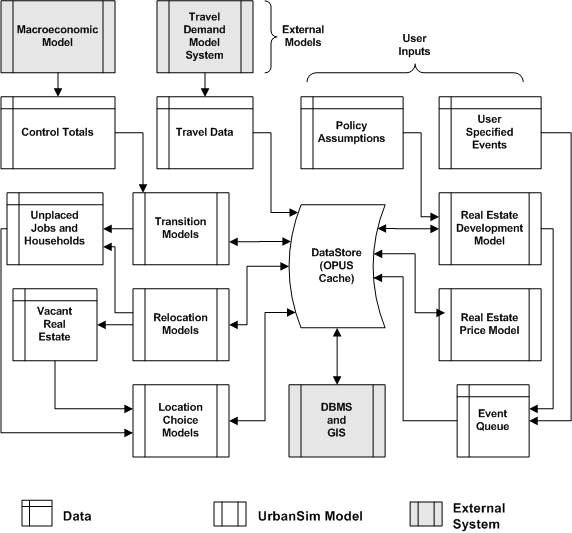
\includegraphics[scale=0.7]{graphics/flow-2008.png}
\end{center}
\caption{UrbanSim Model Components and Data Flow}
\label{fig:dataflow}
\end{figure}

UrbanSim predicts the evolution of these objects and their characteristics over time, using annual steps to predict the movement and location choices of businesses and households, the development activities of developers, and the impacts of governmental policies and infrastructure choices.  The land use model is interfaced with a metropolitan travel model system to deal with the interactions of land use and transportation. Access to opportunities, such as employment or shopping, are measured by the travel time or cost of accessing these opportunities via all available modes of travel.

The data inputs and outputs for operating the UrbanSim model are shown in Table \ref{tab:inputs-outputs}.  Developing the input database is challenging, owing to its detailed data requirements.  A GIS is required to manage and combine these data into a form usable by the model, and can also be used to visualize the model results.  Once the database is compiled, the model equations must be calibrated and entered into the model.  A final step before actual use of the model is a validation process that tests the operation of the model over time and makes adjustments to the dynamic components of the model.  The steps of data preparation, model estimation, calibration and validation will be addressed in later chapters.  In the balance of this chapter the design and specification of UrbanSim, using the most recent parcel-based approach used in the Puget Sound, is presented in more detail.

\begin{table}[htp]
\caption{Data Inputs and Outputs of UrbanSim}
\label{tab:inputs-outputs}
\begin{center}
\begin{tabular}{ p{1.5in}  p{4.4in}  }
%\addlinespace
\toprule[1.5pt]
\multirow{9}{1.5in}{UrbanSim Inputs}
&   $\bullet$ Employment data, in the form of geocoded business establishments\\
%\cmidrule{2-2}
&   $\bullet$ Household data, merged from multiple census sources\\
 %\cmidrule{2-2}
&   $\bullet$  Parcel database, with acreage, land use, housing units, nonresidential square footage, year built, land value, improvement value, city and county\\
 %\cmidrule{2-2}
&   $\bullet$  City and County General Plans\\
 %\cmidrule{2-2}
&   $\bullet$  GIS Overlays for environmental features such as wetlands, floodways, steep slopes, or other sensitive or regulated lands\\
 %\cmidrule{2-2}
&   $\bullet$  Traffic Analysis Zones\\
 %\cmidrule{2-2}
&   $\bullet$   GIS Overlays for any other planning boundaries\\
 %\cmidrule{2-2}
&   $\bullet$  Travel Model outputs\\
 %\cmidrule{2-2}
&  $\bullet$   Development Costs \\
\midrule
\multirow{6}{1.5in}{UrbanSim Outputs (by Building, Parcel or Gridcell), Generally Summarized by Zone}
& $\bullet$    Households by income, age, size, and presence of children\\
 %\cmidrule{2-2}
& $\bullet$    Employment by industry and land use type\\
%\cmidrule{2-2}
& $\bullet$    Acreage by land use\\
 %\cmidrule{2-2}
& $\bullet$    Dwelling units by type\\
 %\cmidrule{2-2}
& $\bullet$    Square feet of nonresidential space by type\\
 %\cmidrule{2-2}
& $\bullet$    Real estate prices\\
\midrule
\multirow{4}{1.5in}{Travel Model Outputs (Zone-to-Zone) Used in UrbanSim}
& $\bullet$    Travel time by mode by time of day by purpose\\
 %\cmidrule{2-2}
& $\bullet$  Trips by mode by time of day by purpose\\
 %\cmidrule{2-2}
& $\bullet$    Composite utility of travel using all modes by purpose \\
%\cmidrule{2-2}
& $\bullet$  Generalized costs (time + time equivalent of tolls) by purpose \\
\bottomrule
\end{tabular}
\end{center}
\end{table}

\section{Policy Scenarios}

UrbanSim is designed to simulate and evaluate the potential effects of multiple scenarios.  We use the term scenario in the context of UrbanSim in a very
specific way: a scenario is a combination of input data and assumptions to the model system, including macroeconomic assumptions regarding the growth of population and employment in the study area, the configuration of the transportation system assumed to be in place in specific future years, and
general plans of local jurisdictions that will regulate the types of development allowed at each location.

In order to facilitate comparative analysis, a model user such as a Metropolitan Planning Organization will generally adopt a specific scenario as a base of comparison or all other scenarios.  This base scenario is generally referred to as the `baseline' scenario, and this is usually based on the adopted or most
likely to be adopted regional transportation plan, accompanied by the most likely assumptions regarding economic growth and land use policies.  Once a  scenario is created, it determines several inputs to UrbanSim:

\squishlist
\item Control Totals: data on the aggregate amount of population and employment, by type, to be assumed for the region.
\item Travel Data: data on zone to zone travel characteristics, from the travel model.
\item Land Use Plan: data on general plans, assigned to individual parcels.
\item Development Constraints: a set of rules that interpret the general plan codes, to indicate the allowed land use types and density ranges on each parcel.
\squishend

\section{Data Structures in UrbanSim}
UrbanSim has evolved over several years, and so have the data structures used in it.  Until 2005, most applications used a data structure based on a grid overlaid on the study area.  Most UrbanSim applications do date have used this approach to structuring the data.  Various limitations of the gridcell approach led to the more recent adoption of a parcel-based data structure.  This section explains the fundamental differences in these data structures, and assesses their relative merits.  Both are still used and supported approaches, though the advantages of the parcel approach are fairly significant.

In this chapter, the Puget Sound model application is used extensively as the basis for the description, in order to make the discussion more tangible\footnote{This does not restrict the generalizability of the results, since the model has been widely adapted to multiple metropolitan areas in North America, Europe and Asia.}.  The study area for the Puget Sound model, now being brought into operational use by the Puget Sound Regional Council (PSRC), is the Central Puget Sound, consisting of King, Kitsap, Pierce and Snohomish Counties in Washington, as shown in Figure \ref{fig:puget-sound}.

\begin{figure}
\begin{center} 

\includegraphics[scale=0.4]{graphics/psrc-p1.jpg}
\end{center}
\caption{Puget Sound Region} 
\label{fig:puget-sound}
\end{figure}

\subsection{Gridcell-based Data Structure}

The gridcell-based approach to developing the data for UrbanSim, as the name suggests, begins with the decision of a resolution to use for a grid to overlay the study area.  There is no definitively correct grid cell resolution, and a pragmatic choice of 150 meters by 150 meters was chosen in early UrbanSim
applications, mainly as a compromise between the high level of resolution desired, and the increased computational demands made by higher resolution data.

Figure \ref{fig:gridcells} depicts a portion of the study area in the Puget Sound, and shows the 150 meter grid initially used for the PSRC model application
superimposed on other planning geographies for relative comparison.  It is obvious that grid cells bisect parcels, or to put it another way, that it is not possible to aggregate parcel information neatly into gridcells.  This was an unfortunate but obvious outcome of imposing a completely regular shape (a grid) on a polygonal layer of parcels that vary in size in shape.  The main advantage of using a grid is that is makes it possible
to use raster processing efficiently, as is done in image processing or raster GIS spatial analysis.  It is possible to compute quite efficiently, for example, how much population or employment is within a fixed radius of each cell.  This computational efficiency was the main initial motivation for using the gridcell approach to structuring the input data for UrbanSim.

\begin{figure}[htp]
\begin{center}
%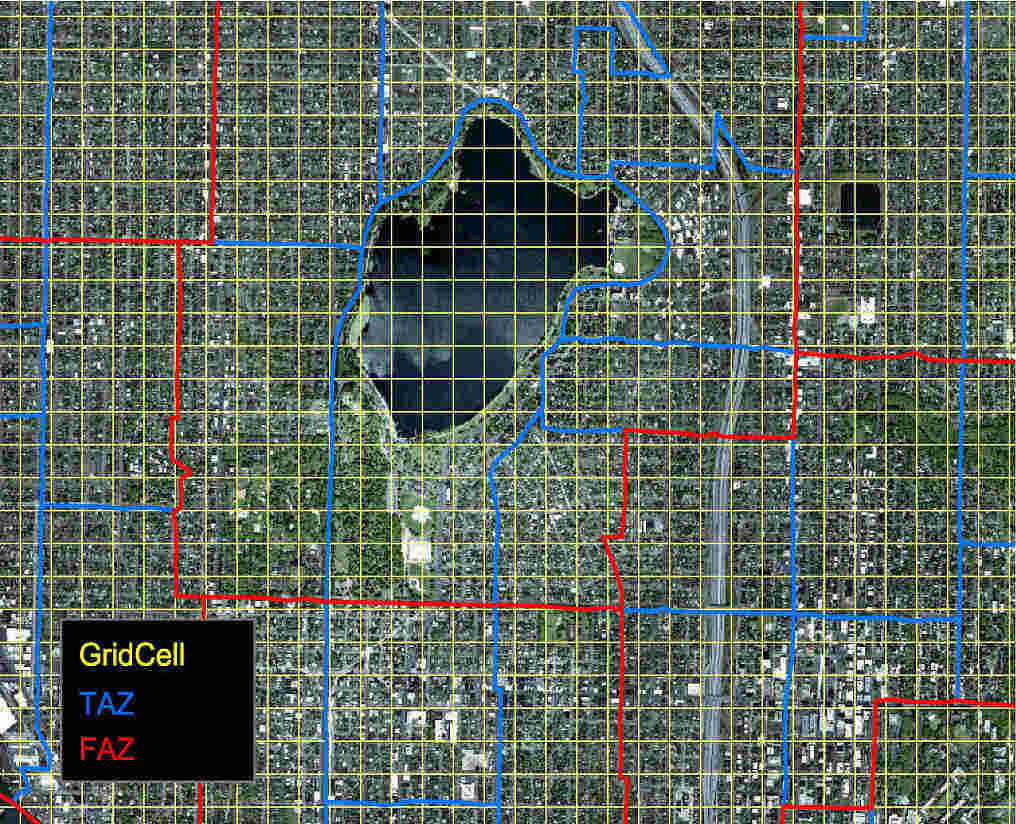
\includegraphics[scale=0.5]{graphics/grid-greenlake.jpg}
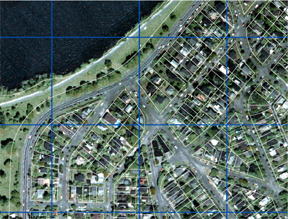
\includegraphics[scale=1.25]{graphics/gridmap-small.png}
\end{center}
\caption{Gridcells in Greenlake Area of Seattle}
\label{fig:gridcells}
\end{figure}

Each gridcell contains approximately 5 1/2 acres, at a resolution of 150 meters.  In order to prepare the data for UrbanSim, parcel maps were overlaid in the GIS on a vector representation of gridcells, and the contents of the parcel (housing, etc)  allocated to the gridcells in proportion to the amount of its land area falling within each gridcell.  The fragments of the real estate components created in this way were then aggregated into a composite at the cell level.  UrbanSim then operates on the gridcell-level data.  In order to better reflect the contents of the grid cells, which are clearly not homogeneous in their composition, building objects were created to allow at least different types of real estate in a cell to be represented by different types of buildings.  Households and jobs were then associated with buildings, and buildings with gridcells, as shown in Figure \ref{fig:grid-data-model}.

\begin{figure}[htp]
\center \resizebox{0.3
\textwidth}{!}{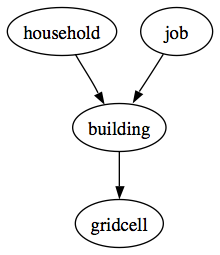
\includegraphics{graphics/grid-data-model.png}}
\caption{Core of Gridcell-based UrbanSim Data Model} \label{fig:grid-data-model}
\end{figure}

The main disadvantage of the gridcell data structure has already been mentioned: it requires unnaturally splitting the underlying parcel information and
recombining it in ways that create artificial representations of the data.  This problem also makes it difficult to apply information on development regulations
from general plans, since those are also based on polygons, and in fact, apply to parcels.

\subsection{Parcel-based Data Structure}

To address some of the limitations of the gridcell-based data structure, recent development of UrbanSim has adopted a data structure based on parcels.
The parcel-based UrbanSim application uses a data model that reflects parcels, buildings, households and jobs as the
primary objects and units of analysis.  Households and jobs
choose locations by selecting a specific building, which is associated with a specific parcel.
Real estate development is based on development projects occurring on specific parcels.  In the most recent extensions of the Puget Sound model,
persons have been added to the data model, and workers are associated with specific jobs.  These data relationships
are shown in Figure \ref{fig:data-model-2}.

\begin{figure*}[h]
\center \resizebox{0.3
\textwidth}{!}{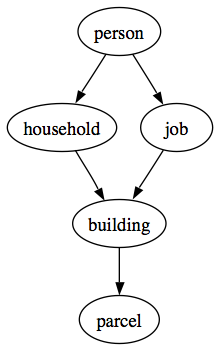
\includegraphics{graphics/data-model-2.png}}
\caption{Core of Parcel-based UrbanSim Data Model} \label{fig:data-model-2}
\end{figure*}


Data from the four counties that comprise the Central Puget Sound - King, Kitsap, Pierce, and Snohomish, shown in Figure \ref{fig:puget-sound} - were assembled to create a year 2000 database\footnote{2001 parcel data were obtained from the assessor files for each county, since there are considerable lags in updating these data
and also due to some significant gaps in the 2000 data from Snohomish County}.  Over 1.2 million parcels are represented in the UrbanSim database
for the Puget Sound, containing over 1 million buildings, almost 1.4 million residential units, and over 1 billion square feet of non-residential space.  Individual building records were separately obtained from two of the counties (King and Snohomish), and were created from
the parcel data attributes for the other two counties.  Attributes of the core datasets are shown in Table \ref{tab:parcel-attributes}. Attributes of the core datasets are shown in Table \ref{tab:parcel-attributes}.

\begin{table}
\caption{Attributes of Core Datasets Used in Puget Sound Parcel-based UrbanSim Application}
%\addlinespace
\label{tab:parcel-attributes}
\begin{tabular}{p{3cm}p{2.8cm}p{2.7cm}p{2.5cm}p{2.5cm}}
\toprule
Parcels & Buildings & Households    & Persons & Jobs \\
\midrule
parcel\_id  & non\_residential\_sqft    & household\_id & person\_id & job\_id \\
tax\_exempt\_flag & year\_built & income    & household\_id & sector\_id\\
parcel\_sqft\_in\_gis & parcel\_id  & persons    & member\_id & join\_flag\\
x\_coord\_sp &  land\_area  & workers & relate & sqft\\
y\_coord\_sp    & building\_quality\_id & children &    age & taz\_est\\
x\_coord\_utm   & improvement\_value    & building\_size    & sex & building\_type\\
y\_coord\_utm   & stories   & tenure    & edu & building\_id\\
grid\_id    & tax\_exempt   & race\_id & age\_of\_head  \\
zone\_id    & building\_type\_id    & employment\_status & race\_id &\\
census\_block   &  building\_id & building\_id & work\_at\_home &\\
city\_id    & template\_id  & & earning & \\
county\_id   &  sqft\_per\_unit & & job\_id & \\
id\_parcel  & & & &\\
id\_plat & & & &\\
is\_inside\_urban\_growth\_boundary & & & & \\
residential\_units  & & & & \\
plan\_type\_id & & & &\\
plan\_type\_description & & & &\\
num\_building\_records & & & &\\
GenericLandUse1 & & & &\\
land\_use\_type\_id & & & &\\
land\_value & & & &\\
parcel\_sqft & & & &\\
faz\_id & & & &\\
large\_area\_id & & & &\\
zipcode & & & &\\
zip\_id & & & &\\
\bottomrule
\end{tabular}
\end{table}



This data structure includes a representation of each individual person, household, job, building and parcel
in the entire metropolitan area, and their associations, meaning, for example, which building each household occupies, and which parcel each building
is on.  This is a `microsimulation' data structure, and makes it straightforward to model choices or changes in the status of any individual agent or
object.  It also makes it possible to summarize output from the model with a great deal of flexibility.  A spatial hierarchy is also used in the data
model to allow aggregation and disaggregation of information across multiple spatial levels.  Parcels are associated with zones (used in the travel
model), gridcells, Forecast Analysis Zones (FAZ), Large Areas (districts used for analysis of results), census blocks, cities, counties, and zip codes.  This
means that it is straightforward to aggregate or query information such as how many households of each income are in each zone, for example, or what
the employment density is within a FAZ.  We can also use these spatial relationships to assign information about travel conditions, predicted by the travel
model on a zone to zone basis, with households, jobs, and locations by using the zone level of geography.  These relationships are shown in Figure
\ref{fig:geographic-relationships}.

\begin{figure*}
\center \resizebox{0.9
\textwidth}{!}{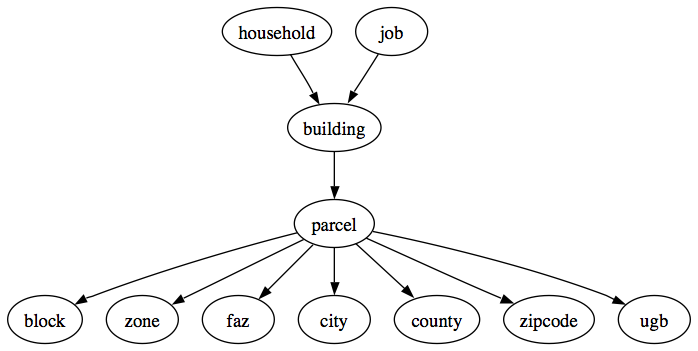
\includegraphics{graphics/geographic-relationships.png}}
\caption{Spatial Relationships Among Core UrbanSim Entities} \label{fig:geographic-relationships}
\end{figure*}

The land use and building type coding systems used by each of the counties were not consistent
with each other, so a more general classification was created that would allow the use of a uniform typology across the region.  These land use
types are shown in Table \ref{tab:landuse}.  Buildings are classified also, using a generic building type that approximates the generic lans use type (they cannot be identical, since there are more land uses to describe vacant land and other uses), along with a somewhat more detailed building type.  A profile
of buildings in the Puget Sound database, and their classification, is shown in Table \ref{tab:buildings}.



\begin{table}
\begin{center}
\caption{Generic Land Use Codes}
%\addlinespace
\label{tab:landuse}
\begin{tabular}{{l}p{3.5cm}}
\toprule
1   & single\_family\_residential\\
2   & multi\_family\_residential\\
3   & office\\
4   & commercial\\
5   & industrial\\
6   & mixed\_use\\
7   & government\\
8   & other\\
9   & no code\\
\bottomrule
\end{tabular}
\end{center}
\end{table}

\begin{table}
\begin{center}
\caption{Building Types and Characteristics in Central Puget Sound}
%\addlinespace
\label{tab:buildings}
\begin{tabular}{p{1cm}p{3cm}p{2cm}{r}{r}{r}}
\toprule
Building Type Id    & Description   & Generic Building Type & Frequency & Residential Units &   Non-res Sqft (000) \\
\midrule
1   & Agriculture   & other & 1,702 & 4 & 6,923\\
2   & Civic and Quasi-Public &  government  & 2,574 & 212   & 26,821\\
3   & Commercial    & commercial    & 19,272    & 2,181 & 210,751\\
4   & Condo Residential & multi-family residential &    9,829   & 132,678   & 0\\
5   & Government    & government    & 847   & 72    & 71,410\\
6   & Group Quarters    & other &   391 & 6,893 & 3,856\\
7   & Hospital / Convalescent Center    & government    & 715   & 118   & 21,407\\
8   & Industrial    & industrial    & 3,783 & 85    & 91,254\\
9   & Military &    government  & 10    & 4 & 32\\
10  & Mixed-Use & mixed-use & 529   & 1,562 & 2,580\\
11  & Mobile Home   & single family residential & 26,691    & 26,691    & 0\\
12  & Multi-Family Residential  & multi-family residential  & 45,215    & 317,612   & 52,784\\
13  & Office    & office    & 10,713    & 1,434 & 193,696\\
14  & Outbuilding   & other  & 37,789   & 519   & 29,312\\
15  & Park and Open Space   & other &   7 & 0   & 564\\
16  & Parking   & other & 1,043 & 150   & 25,606\\
17  & Recreation &  other   & 1,407 & 2,138 & 12,560\\
18  & School    & other &   2,678   & 192   & 57,487\\
19  & Single Family Residential & single family residential & 818,703   & 893,328   & 992\\
20  & Transportation Communication Utilities    & industrial    & 1,319 & 199   & 10,389\\
21  & Warehousing   & industrial    & 10,138    & 756   & 228,374\\
22  & No Code   & other &   13,788  & 3,864 & 8,681\\
\midrule
Total & & & 1,009,143   & 1,390,692 &   1,055,489\\
\bottomrule
\end{tabular}
\end{center}
\end{table}


The parcel and building data used in UrbanSim allow for representation of mixed use development, with multiple buildings per parcel.  Representation
of a single mixed use building can be accommodated by using two building components, each of a single use, and both associated with the same
parcel.

\section{Interface with Travel Model}

UrbanSim takes several key inputs as exogenous, meaning that these
are input assumptions that are not predicted directly by UrbanSim.  Two of these are
from external model systems: a macroeconomic model to predict
future macroeconomic conditions such as population and employment
by sector, and a travel demand model system to predict travel
conditions such as congested times and composite utilities of
travel between each interchange.  The latter is loosely coupled to
UrbanSim, with land use predictions input to the external travel
models, and travel conditions input to subsequent annual
iterations of the UrbanSim land use model system.

The travel models in widespread use in Metropolitan Planning Organizations are
almost all traditional four-step travel models.  The first model in the process
is the trip generation model, and this uses zonal population and employment
characteristics.  When UrbanSim is connected to a travel model system,
it generates a summary of the household and job data to a zone level, in order
to create the summary input data needed by the travel model.

When the travel model completes the fourth step of traffic assignment to a
transportation network, it can produce `skims' from zone to zone that summarize
key model predictions, such as:

\squishlist
\item   Travel time by mode by time of day by purpose
\item Trips by mode by time of day by purpose
\item   Composite utility of travel using all modes by purpose
\item Generalized costs (time + time equivalent of tolls) by purpose
\item Logsums, or composite utilities\footnote{See section \ref{sec:discrete-choice} for an explanation of this measure.}, from the mode choice model, by purpose and time of day
\squishend

These skims can be combined with the spatial information in UrbanSim regarding the location of households and jobs, to produce
a variety of accessibility measures, which in turn can influence UrbanSim models of residential location, workplace location, employment
location, real estate prices, and real estate development.  Figure \ref{fig:TMinterface} summarizes the interactions between UrbanSim and
the travel model system.

\begin{figure*}[h]
\center \resizebox{0.5
\textwidth}{!}{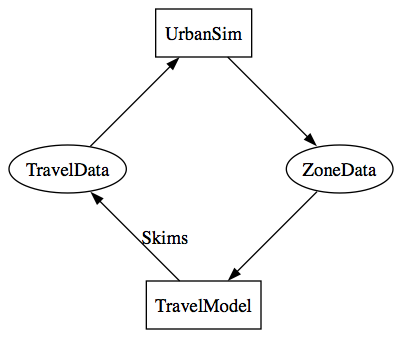
\includegraphics{graphics/travel-model-interface.png}}
\caption{UrbanSim - Travel Model Interface} \label{fig:TMinterface}
\end{figure*}

In some applications, such as the San Francisco model, the travel model system is based on a more sophisticated activity-based
framework, and UrbanSim is interfaced in a similar way. In the future, potential exists to more closely integrate UrbanSim with
Activity-based models that are moving from research into practice.

\section{UrbanSim Model Components}

The models used in the parcel version of UrbanSim differ in some obvious respects from the earlier gridcell versions, and these are summarized in Table \ref{tab:components-parcel}.  In addition to the substitution of parcels for gridcells as the unit of analysis, the real estate development model was completely restructured to take advantage of the availability of parcel geography in representing actual development projects - which do vary in size and shape in the real world, in ways that were difficult to reconcile with gridcell geography.  The parcel based model specifications also have recently added models to predict the choice of workers to be home-based (normally work from home), and a workplace choice model for workers who are not home-based.  This allows for the first time the more appropriate handling of the prediction of commuting behavior as a long-term outcome of where a household chooses to live, and where the workers in the household have jobs, and allows the removal of the home-based-work trip distribution model from the set of behaviors predicted by the travel model on a daily basis.

\begin{table}[htp]
\caption{Specification of UrbanSim Model Components}
\label{tab:components-parcel}
%\begin{tabular*}{6in}{@{\extracolsep{\fill}}  p{5cm} | p{.2cm} | p{2cm} | p{2.5cm} | p{2cm} | }
\begin{tabular}{p{4.5cm} p{3.4cm}p{3.4cm}p{3.3cm}}
\toprule[1.5pt]
Model & Agent & Dependent Variable & Functional Form \\
\midrule
Household Location Choice & Household (New or Moving) & Residential Building With Vacant Unit & Multinomial Logit \\
\midrule
Employment Location Choice & Job (New or Moving) & Non-residential Building With Vacant Space & Multinomial Logit \\
\midrule
Home-based Job Choice & Worker (Without Job) & Binary Choice (Work at Home) & Binary Logit \\
\midrule
Workplace Choice & Non Home Based Worker (Without Job) & Vacant Job & Multinomial Logit \\
\midrule
Real Estate Development  & Development Proposal & Parcel (With Vacant Land) & Multinomial Logit Sampler \\
\midrule
Real Estate Price & Parcel & Price Per Square Foot & Multiple Regression \\
\bottomrule[1.5pt]
\end{tabular}
\end{table}


In the remainder of this chapter, the components of the current parcel version of UrbanSim,
as applied in the Puget Sound application, are described in some detail in terms of their
structure and algorithms.  Since many (but not all) of these models are based on a discrete choice framework,
a brief explanation of the common basis for these models is presented first.

\subsection{Discrete Choice Models}
\label{sec:discrete-choice}

A pathbreaking approach to modeling individual actions using discrete
choice models emerged in the 1970's, with the pioneering work of
McFadden on Random Utility Maximization theory
\cite{mcfadden-1974,mcfadden-1981}. This approach derives a model of
the probability of choosing among a set of available alternatives
based on the characteristics of the chooser and the attributes of
the alternative, and proportional to the relative utility that the
alternatives generate for the chooser. Maximum likelihood and
simulated maximum likelihood methods have been developed to estimate
the parameters of these choice models from data on revealed or
stated preferences, using a wide range of structural specifications
(see \cite{train-book-2003}). Early application of these models were
principally in the transportation field, but also included work on
residential location choices
\cite{quigley-eer-1976,lerman-trr-1977,mcfadden-1978}, and
on residential mobility \cite{clark-vanlierop-1986}.

Let us begin with an example of a simple model of households choosing among
alternative locations in the housing market, which we index by
$i$. For each agent, we assume that each alternative $i$ has
associated with it a utility $U_i$ that can be separated into a
systematic part and a random part:
\begin{equation}
    U_i = V_i + \epsilon_i,
    \label{eq:utility}
\end{equation}
%$V_i = \vk{\beta}\cdot\vk{x}_i$
where $V_i = \beta\cdot {x}_i$ is a linear-in-parameters
function, $\beta$ is a vector of $k$ estimable coefficients,
$x_i$ is a vector of observed, exogenous, independent
alternative-specific variables that may be interacted with the
characteristics of the agent making the choice, and $\epsilon_i$
is an unobserved random term. Assuming the unobserved term in
(\ref{eq:utility}) to be distributed with a Gumbel distribution
leads to the  widely used multinomial logit model
\cite{mcfadden-1974,mcfadden-1981}:
\begin{equation}
    P_i = \frac{\mathrm{e}^{V_i}}{\sum_j \mathrm{e}^{V_j}},
    \label{eq:mnl}
\end{equation}
where $j$ is an index over all possible alternatives. The
estimable coefficients of (\ref{eq:mnl}), $\beta$, are
estimated with the method of maximum likelihood (see for example
\cite{Greene-2002}).

The denominator of the equation for the choice model has a particular
significance as an evaluation measure.  The log of this denominator
is called the \emph{logsum}, or composite utility, and it summarizes
the utility across all the alternatives.  In the context of a choice of
mode between origins and destinations, for example, it would summarize
the utility (disutility) of travel, considering all the modes connecting the
origins and destinations.  It has theoretical appeal as an evaluation
measure for this reason.  In fact, the logsum from the mode choice
model can be used as a measure of accessibility.

\begin{figure}[htp]
\center
 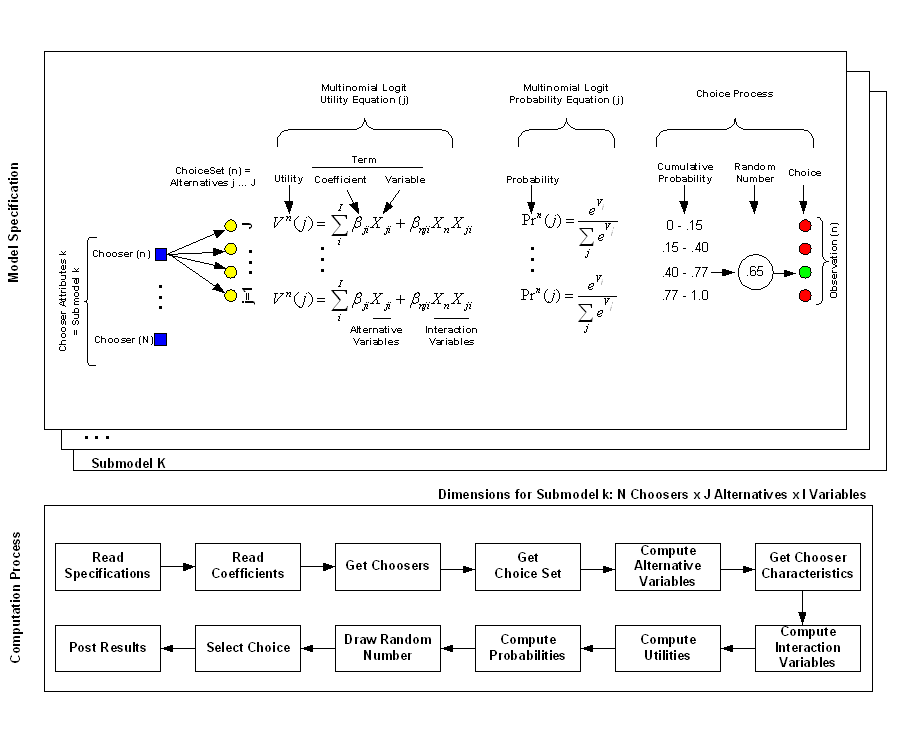
\includegraphics[width=6.5in]
 {graphics/ChoiceProcess.png}
\caption{Computation Process in UrbanSim Choice Models}
\label{fig:choiceprocess}
\end{figure}

Choice models are implemented in UrbanSim in a modular way, to allow flexible specification of models
to reflect a wide variety of choice situations.  Figure \ref{fig:choiceprocess} shows the process both in the form
of the equations to be computed, and from the perspective of the tasks implemented as methods in software.

For each model component within the UrbanSim model system, the
choice process proceeds as shown in Figure
\ref{fig:choiceprocess}. The first steps of the model read the
relevant model specifications and data.  Then a choice set is
constructed for each chooser.  Currently this is done using random
sampling of alternatives, which has been shown to generate consistent, though not
efficient, estimates of model parameters \cite{ben-akiva-lerman-1987}.

The choice step in this algorithm warrants further explanation.  Choice models predict choice probabilities, not choices.
In order to predict choices given the predicted probabilities, we require an algorithm to select a specific choice outcome.
A tempting approach would be to select the alternative with the maximum probability, but unfortunatelty this strategy
would have the effect of selecting only the dominant outcome, and less frequent alternatives would be completely
eliminated.  In a mode choice model, for illustration, the transit mode would disappear, since the probability of choosing
an auto mode is almost always higher than that of choosing transit.  Clearly this is not a desirable or realistic outcome.
In order to address this problem, the choice algorithm used for choice models uses a sampling approach.  As illustrated in Figure
\ref{fig:choiceprocess}, a choice outcome can be selected by sampling a random number from the uniform distribution in the range
0 to 1, and comparing this random draw to the cumulative probabilities of the alternatives.  Whichever alternative the sampled
random number falls within is the alternative that is selected as the `chosen' one.  This algorithm has the property that it
preserves in the distribution of choice outcomes a close approximation of the original probability distribution, especially
as the sample size of choosers becomes larger.

One other choice context is worth noting.  In some situations, the availability of alternatives may be constrained.  If the limit on availability
is entirely predictable, such as a budget constraint eliminating expensive options, or a zero-car household being unable to use the drive-alone
mode, this is straightforward to handle, by eliminating the alternatives from the choice set for those choosers.  In other situations, however, the
solution is not so straightforward.  In the case where alternatives may be unavailable because many other agents wish to choose them, the problem
is that the alternative may be unavailable due to the endogenous congestion of alternatives.  The effect of this is potentially significant, since it
may cause parameters estimated in a choice model to confuse, or confound, the effects of preferences with the effects of constraints.  Fortunately,
an estimation method has been developed to account for this problem \cite{depalma-jue-2007}.

\subsection{Economic Transition Model}
Employment is classified by the user into employment sectors based
on aggregations of Standard Industrial Classification (SIC) codes, or more
recently, North American Industry Classification (NAICS) codes.
Typically 10 to 20 sectors are defined based on the local economic
structure. Aggregate forecasts of economic activity and sectoral
employment are exogenous to UrbanSim, and are used as inputs to
the model. These forecasts may be obtained from state economic
forecasts or from commercial or in-house sources.

The base year UrbanSim employment data for the
Puget Sound application are derived from data from the State of Washington
Employment Securities Division, generally referred to
as ES202 data, containing unemployment insurance administrative
records with information on the location and size of business
establishments.  InfoUSA is a commonly used private source for
similar data, compiled from credit reports and other sources.

The Economic Transition Model integrates exogenous forecasts
of aggregate employment by sector with the UrbanSim database by
computing the sectoral growth or decline from the preceding year,
and either removing jobs from the database in sectors that are
declining, or queuing jobs to be placed in the employment location
choice model for sectors that experience growth.  If the user
supplies only total employment control totals, rather than totals
by sector, the sectoral distribution is assumed consistent with
the current sectoral distribution. In cases of employment loss,
the probability that a job will be removed is assumed proportional
to the spatial distribution of jobs in the sector.  The jobs that
are removed vacate the space they were occupying, and this space
becomes available to the pool of vacant space for other jobs to
occupy in the location component of the model.  This procedure
keeps the accounting of land, structures, and occupants up to
date.

New jobs are not immediately assigned a location.  Instead, new
jobs are added to the database and assigned a null location, to be
resolved by the Employment Location Choice Model.


\subsection{Demographic Transition Model}

The Demographic Transition Model accounts for changes in the
distribution of households by type over time, using an algorithm
analogous to that used in the Economic Transition Model.  In
reality, these changes result from a complex set of social and
demographic changes that include aging, household formation,
divorce and household dissolution, mortality, birth of children,
migration into and from the region, changes in household size, and
changes in income, among others.  The data (and theory) required
to represent all of these components and their interactions
adequately are complex, and this set of behaviors remain to be
implemented in UrbanSim. Instead, the Demographic
Transition Model, like the Economic Transition Model described
above, uses external control totals of population and households
by type (the latter only if available) to provide a mechanism for
the user to approximate the net results of these changes. Analysis
by the user of local demographic trends may inform the
construction of control totals with distributions of household
size, age of head, and income.  If only total population is
provided in the control totals, the model assumes that the
distribution of households by type remains static.

As in the economic transition case, household births are added to
a list of movers that will be located by the Household Location
Choice Model.  Household deaths, on the other hand, are accounted
for by this model by removing those households from the housing
stock, and by properly accounting for the vacancies created by
their departure.  The demographic transition model is analogous in
form to the employment transition model described above.


\subsection{Employment Relocation Choice Model}

Employment relocation and location choices are made by firms.
However, in the current version of UrbanSim, we use individual
jobs as the units of analysis.  This is equivalent to assuming
that businesses are making individual choices about the location
of each job, and are not constrained to moving an entire
establishment.

The Employment Relocation Choice Model predicts the probability that jobs
of each type will move from their current location or stay during
a particular year. This is a transitional change that could
reflect job turnover by employees, layoffs, business relocations
or closures. Similar to the economic transition model when
handling job losses in declining sectors, the model assumes that
the hazard of moving is proportional to the spatial distribution
of jobs in the sector.  All placement of jobs is managed through
the employment location model.

As in the case of job losses predicted in the economic transition
component, the application of this model requires subtracting jobs
by sector from the buildings they currently occupy, and the
updating of the accounting to make this space available as vacant
space. These counts will be added to the unallocated new jobs by
sector calculated in the economic transition model. The
combination of new and moving jobs serve as a pool to be located
in the employment location choice model. Vacancy of nonresidential
space will be updated, making space available for allocation in
the employment location choice model.

Since it is possible that the relative attractiveness of
commercial space in other locations when compared with an
establishment's current location may influence its decision to
move, an alternative structure for the mobility model could use
the marginal choice in a nested logit model with a conditional
choice of location. In this way, the model would use information
about the relative utility of alternative locations compared to
the utility of the current location in predicting whether jobs
will move.  While this might be more theoretically appealing than
the specification given, it is generally not supported by the data
available for calibration. Instead, the mobility decision is
treated as an independent choice, and the probabilities estimated
by annual mobility rates directly observed over a recent period
for each sector.


\subsection{Household Relocation Choice Model}

The Household Relocation Choice Model is similar in form to the Employment
Relocation Choice Model described above.  The same algorithm is used, but
with rates or coefficients applicable to each household type.  For
households, mobility probabilities are estimated from the Census
Current Population Survey, which provides a national database on
which annual mobility rates are computed by type of household.
This will reflect differential mobility rates for renters and
owners, and households at different life stages.

Application of the Household Relocation Choice Model requires subtracting
mover households by type from the housing stock by building, and
adding them to the pool of new households by type estimated in the
Demographic Transition Model. In the database, this is
accomplished by setting the location field for the moving
households to a null value.  The combination of new and moving
households serves as a population of households to be located by
the Household Location Choice Model. Housing vacancy is updated as
movers are subtracted, making the housing available for occupation
in the household location and housing type choice model.


\subsection{Employment Location Choice Model}

In this model, we predict the probability that a job that is
either new (from the Economic Transition Model), or has moved
within the region (from the Employment Mobility Model), will be
located at a particular site.  Buildings are used as the basic
geographic unit of analysis in the current model implementation.
Each job has an attribute of space it needs, and this provides
a simple accounting framework for space utilization within
buildings. The
number of locations available for a job to locate within a building
will depend mainly on the total square footage of
nonresidential floorspace in the building, and on the density of the
use of space (square feet per employee).

Given the possibility
that some jobs will be located in residential units, however,
housing as well as nonresidential floorspace must be considered in
job location.  We have allowed the user to specify the control totals
for employment by sector in two categories: home-based and
non-home-based.  The model is specified as a multinomial logit model,
with separate equations estimated for each employment sector.


For both the employment location and household location models, we
take the stock of available space as fixed in the short run of the
intra-year period of the simulation, and assume that locators are
price takers.  That is, a single locating job or household does
not have enough market power to influence the transaction price,
and must accept the current market price as given.

The variables included in the employment location choice model are
drawn from the literature in urban economics.  We expect that
accessibility to population, particularly high-income population,
increases bids for retail and service businesses.  We also expect
that two forms of agglomeration economies influence location
choices: localization economies and inter-industry linkages.

Localization economies represent positive externalities associated
with locations that have other firms in the same industry nearby.
The basis for the attraction may be some combination of a shared
skilled labor pool, comparison shopping in the case of retail,
co-location at a site with highly desirable characteristics, or
other factors that cause the costs of production to decline as
greater concentration of businesses in the industry occurs.  The
classic example of localization economies is Silicon Valley.
Inter-industry linkages refer to agglomeration economies
associated with location at a site that has greater access to
businesses in strategically related, but different, industries.
Examples include manufacturers locating near concentrations of
suppliers in different industries, or distribution companies
locating where they can readily service retail outlets.

One complication in measuring localization economies and
inter-industry linkages is determining the relevant distance for
agglomeration economies to influence location choices.  At one
level, agglomeration economies are likely to affect business
location choices between states, or between metropolitan areas
within a state.  Within a single metropolitan area, we are
concerned more with agglomeration economies at a scale relevant to
the formation of employment centers.  The influence of proximity
to related employment may be measured using two scales: a regional
scale effect using zone-to-zone accessibilities from the travel
model, or highly localized accessibilities using queries of the
area immediately around the given parcel.  Most of the spatial
queries used in the model are of the latter type, because the
regional accessibility variables tend to be very highly
correlated, and because agglomerations are expected to be very
localized.

Age of buildings is included in the model to estimate the
influence of age depreciation of commercial buildings, with the
expectation that businesses prefer newer buildings and discount
their bids for older ones.  This reflects the deterioration of
older buildings, changing architecture, and preferences, as is the
case in residential housing.  There is the possibility that
significant renovation will make the actual year built less
relevant, and we would expect that this would dampen the
coefficient for age depreciation.  We do not at this point attempt
to model maintenance and renovation investments and the quality of
buildings.

Density, the inverse of lot size, is included in the location
choice model.  We expect businesses, like households, to reveal
different preferences for land based on their production functions
and the role of amenities such as green space and parking area. As
manufacturing production continues to shift to more horizontal,
land-intensive technology, we expect the discounting for density
to be relatively high.  Retail, with its concentration in shopping
strips and malls, still requires substantial surface land for
parking, and is likely to discount bids less for density.  We
expect service firms to discount for density the least, since in
the traditional urban economics models of bid-rent, service firms
generally outbid other firms for sites with higher accessibility,
land cost, and density.

We might expect that certain sectors, particularly retail, show
some preference for locations near a major highway, and are
willing to bid higher for those locations.  Distance to a highway
is measured in meters, using grid spatial queries.  We also test
for the residual influence of the classic monocentric model,
measured by travel time to the CBD, after controlling for
population access and agglomeration economies.  We expect that,
for most regions, the CBD accessibility influence will be
insignificant or the reverse of that in the traditional
monocentric model, after accounting for these other effects.

Estimation of the parameters of the model is based on a geocoded establishment file
(matched to the parcel file to link employment by type to land use
by type).  A sample of geocoded jobs in each sector is used to
estimate the coefficients of the location choice model.  As with
the Household Location Choice Model, the application of the model
produces demand by each employment type for building locations.

The independent variables used in the employment location choice
model can be grouped into the categories of real estate
characteristics, regional accessibility, and urban-design scale
effects as shown below:

\begin{itemize}

\item Real Estate Characteristics \\ \emph{Prices} \\
\emph{Development type (land use mix, density)}

\item Regional accessibility \\
\emph{Access to population} \\ \emph{Travel time to CBD, airport}

\item Urban design-scale \\ \emph{Proximity to highway, arterials}

\item Local agglomeration economies within and between sectors: center
formation

\end{itemize}



\subsection{Household Location Choice Model}

In this model, as in the employment location model, we predict the
probability that a household that is either new (from the
transition component), or has decided to move within the region
(from the mobility component), will choose a particular location
defined by a residential building.  As before, the form of the model is
specified as multinomial logit, with random sampling of
alternatives from the universe of available (vacant) housing
units, including those units vacated by movers in the current
year.

The model architecture allows location choice models to be
estimated for households stratified by income level, the presence
or absence of children, and other life cycle characteristics.
Alternatively, these effects can be included in a single model
estimation through interactions of the household characteristics
with the characteristics of the alternative locations.  The
current implementation is based on the latter but is general
enough to accommodate stratified estimation, for example by
household income. The variables used in the model are drawn from
the literature in urban economics, urban geography, and urban
sociology.  An initial feature of the model specification is the
incorporation of the classical urban economic trade-off between
transportation and land cost. This has been generalized to account
not only for travel time to the classical monocentric center, the
CBD, but also to more generalized access to employment
opportunities and to shopping. These accessibilities to work and
shopping are measured by weighting the opportunities at each
destination zone with a composite utility of travel across all
modes to the destination, based on the logsum from the mode choice
travel model.

These measures of accessibility should negate the traditional pull
of the CBD, and, for some population segments, potentially reverse
it.  In addition to these accessibility variables, we include in
the model a net building density, to measure the
input-substitution effect of land and capital.  To the extent that
land near high accessibility locations is bid up in price, we
should expect that builders will substitute capital for land and
build at higher densities.  Consumers for whom land is a more
important amenity will choose larger lot housing with less
accessibility, and the converse should hold for households that
value accessibility more than land, such as higher income
childless households.

The age of housing is considered for two reasons.  First, we
should expect that housing depreciates with age, since the
expected life of a building is finite, and a consistent stream of
maintenance investments are required to slow the deterioration of
the structure once it is built.  Second, due to changing
architectural styles, amenities, and tastes, we should expect that
the wealthiest households prefer newer housing, all else being
equal.  The exception to this pattern is likely to be older,
architecturally interesting, high quality housing in historically
wealthy neighborhoods.  The preference for these alternatives are
accommodated through a combination of nonlinear or dummy variable
treatment for this type of housing and neighborhood.

A related hypothesis from urban economics is that, since housing
is considered a normal good, it has a positive income elasticity
of demand.  This implies that as incomes rise, households will
spend a portion of the gains in income to purchase housing that is
more expensive, and that provides more amenities (structural and
neighborhood) than their prior dwelling.  A similar hypothesis is
articulated in urban sociology in which upward social mobility is
associated with spatial proximity to higher status households.
Both of these hypotheses predict that households of any given
income level prefer, all else being equal, to locate in
neighborhoods that have higher average incomes.  (UrbanSim does
not attempt to operationalize the concepts of social status or
social assimilation, but does consider income in the location
choice.)

The age hypothesis and the two income-related hypotheses are
consistent with the housing filtering model, which explains the
dynamic of new housing construction for wealthy households that
sets in motion a chain of vacancies.   The vacancy chain causes
households to move into higher status neighborhoods than the ones
they leave, and housing units to be successively occupied by lower
and lower status occupants.  At the end of the vacancy chain, in
the least desirable housing stock and the least desirable
neighborhoods, there can be insufficient demand to sustain the
housing stock and vacancies go unsatisfied, leading ultimately to
housing abandonment.  We include in the model an age depreciation
variable, along with a neighborhood income composition set of
variables, to collectively test the housing filtering and related
hypotheses.

Housing type is included in the model as a set of dummy variables
for alternative housing types.  These
are discussed further in Section
\ref{real-estate-development-model} describing the real estate
development model.

One of the features that households prefer is a compatible land
use mix within the neighborhood.  It is likely that residential
land use, as a proxy for land uses that are compatible with
residential use, positively influences housing bids.   On the
other hand, industrial land use, as a proxy for less desirable
land use characteristics, would lower bids.

The model parameters are estimated using a random sample of alternative
locations, which has been shown to provide consistent estimates of
the coefficients.  In application for forecasting, each locating
household is modeled individually, and a sample of alternative
cell locations is generated in proportion to the available
(vacant) housing. Monte carlo simulation is used to select the
specific alternative to be assigned to the household, and vacant
and occupied housing units are updated in the cell.

The market allocation mechanism used to assign households and jobs
to available space, then, is not done through a general
equilibrium solution in which we assume consumers and suppliers
optimize across all alternatives based on perfect information, and
zero transaction costs, with prices on all buildings at each
location adjusting to the general equilibrium solution that
perfectly matches consumers and suppliers to clear the market.
Rather, the solution is based on an expectation of incomplete
information and nontrivial transactions and search costs, so that
movers obtain the highest satisfactory location that is available,
and prices respond at the end of the year to the balance of demand
and supply at each location.

The independent variables can be organized into the three
categories of housing characteristics, regional accessibility, and
urban-design scale effects as shown below.

\begin{itemize}

\item{Housing Characteristics} \\
\emph{Prices (interacted with income) \\
Development types (density, land use mix) Housing age}

\item{Regional accessibility} \\
\emph{Job accessibility by auto-ownership group \\
Travel time to CBD and airport}

\item{Urban design-scale (local accessibility) \\
\emph{Neighborhood land use mix and density \\
Neighborhood Employment}}

\end{itemize}

\subsection{Real Estate Price Model}

UrbanSim uses real estate prices as the indicator of the match between
demand and supply of land at different locations and with
different land use types, and of the relative market valuations
for attributes of housing, nonresidential space, and location.
This role is important to the rationing of land and buildings to
consumers based on preferences and ability to pay, as a reflection
of the operation of actual real estate markets. Since prices enter
the location choice utility functions for jobs and households, an
adjustment in prices will alter location preferences.  All else
being equal, this will in turn cause higher price alternatives to
become more likely to be chosen by occupants who have lower price
elasticity of demand. Similarly, any adjustment in land prices
alters the preferences of developers to build new construction by
type of space, and the density of the construction.

We make the following assumptions:

\begin{enumerate}
\item Households, businesses, and developers are all
price-takers, and market adjustments are made by the market in
response to aggregate demand and supply relationships.  Each
responds, therefore, to previous period price information.

\item
Location preferences and demand-supply imbalances are capitalized
into land values.  Building value reflects building replacement
costs only, and can include variations in development costs due to
terrain, environmental constraints or development policy.

\item
There is a long-term structural vacancy rate for each type of
property, and the relationship of current vacancy rates to this
long-term vacancy rate influences price adjustments.
\end{enumerate}

Real estate prices are modeled using a hedonic regression of the log-transformed
property value per square foot
on attributes of the parcel and its environment, including land use
mix, density of development, proximity of highways and other
infrastructure, land use plan or zoning constraints, and
neighborhood effects.  The hedonic regression may be estimated
from sales transactions if there are sufficient transactions on
all property types, and if there is sufficient information on the
lot and its location.  An alternative is to use tax assessor
records on land values, which are part of the database typically
assembled to implement the model.  Although assessor records may
contain biases in their assessment, they do provide virtually
complete coverage of the land (with notable exceptions and gaps
for exempt or publicly owned property).

The hedonic regression equation encapsulates interactions between
market demand and supply, revealing an envelope of implicit
valuations for location and structural characteristics \cite{dipasquale-wheaton-1996}.
Prices are updated by UrbanSim annually, after all construction and market
activity is completed.  These end of year prices are then used as
the values of reference for market activities in the subsequent
year.

The independent variables influencing land prices can be organized
into site characteristics, regional accessibility, and urban-design
scale effects, as shown below:

\begin{itemize}

\item Site characteristics \\
\emph{Development type \\
Land use plan \\
Environmental constraints}

\item Regional accessibility \\
\emph{Access to population and employment}

\item Urban design-scale \\
\emph{Land use mix and density \\
Proximity to highway and arterials}

\end{itemize}

\subsection{Real Estate Development Model}
\label{real-estate-development-model}

\emph{WARNING: THIS SECTION STILL NEEDS TO BE UPDATED}

Constraints on development outcomes are included through a
combination of user-specified spatial overlays and decision rules
about specific types of development allowed in different
situations.  First, each parcel is assigned a series of overlays
through spatial preprocessing using GIS overlay techniques.  These
overlays include features such as the following:

\begin{itemize}
\item  Land use plan designation
\item  City
\item  County
\item  Wetland designation
\item  Floodplain/floodway
\item  Stream or riparian buffer
\item  High slope areas
\item  Urban Growth Boundary
\end{itemize}


These overlays can be used to assign user-specified constraints on
the type of development that is allowed to occur within each of
these overlay designations.  These constraints are interpreted as
'binding' constraints, and not subject to
market pressure. Currently, if users wish to examine the impact of
these constraints, they would need to 'relax' a particular
constraint within one scenario and compare the scenario results to
a more restrictive policy.

The independent variables used in the real estate development
model can be organized into categories of site characteristics,
urban design-scale effects, regional accessibility, and market
conditions, as shown below:

\begin{itemize}
\item Site characteristics \\
\emph{Existing development characteristics \\
Land use plan \\
Environmental constraints}

\item Urban design-scale \\
\emph{Proximity to highway and arterials \\
Proximity to existing development \\
Neighborhood land use mix and property values \\
Recent development in neighborhood}

\item Regional accessibility \\
\emph{Access to population and employment \\
Travel time to CBD, airport}

\item Market Conditions \\
\emph{Vacancy rates}
\end{itemize}

\subsection{The Role of Accessibility}

Accessibility is a very important influence in urban space, and it
similarly plays an important role in UrbanSim.  Almost all models
in UrbanSim consider the effects of accessibility.  But unlike
the monocentric or spatial interaction models, in which the choice
of workplace is exogenous and
residential locations are chosen principally on the basis of
commute to the city center or to a predetermined workplace, we
deal with accessibility in a more general framework. Accessibility
is considered a normal good, like other positive attributes of
housing, which consumers place a positive economic value on.  We
therefore expect that consumers value access to workplaces and
shopping opportunities, among the many other attributes they
consider in their housing preferences. However, not all households
respond to accessibility in the same way. Retired persons would be
less influenced by accessibility to job opportunities than would
working age households, for instance.

We operationalize the concept of accessibility for a given
location as the distribution of opportunities weighted by the
travel impedance, or alternatively the utility of travel to those
destinations.  A number of alternative accessibility measures have
been developed in UrbanSim. The utility of travel is measured as the composite
utility across all modes of travel for each zone pair, obtained as
the logsum of the mode choice for each origin-destination pair.

The accessibility model reads the logsum matrix from the travel
model and the land use distribution for a given year, and creates
accessibility indices for use in the household and business
location choice models. The general framework is to summarize the
accessibility from each zone to various activities for which
accessibility is considered important in household or business
location choice.

Since UrbanSim operates annually, but travel model updates are
likely to be executed for two to three of the years within the
forecasting horizon, travel utilities remain constant from one
travel model run until they are replaced by the next travel model
result. Although travel utilities remain constant, the activity
distribution in these accessibility indices is updated annually,
so that the accessibility indices change from one year to the next
to reflect the evolving spatial distribution of activities.

\subsection{User-Specified Events}

Given our current understanding, no model will be able to simulate
accurately the timing, location and nature of major events such as
a major corporate relocation into or out of a metropolitan area,
or a major development project such as a regional shopping mall.
In addition, major policy events, such as a change in the land use
plan or in an Urban Growth Boundary, are outside the range of
predictions of our simulation.  (At least in its current form,
UrbanSim is intended as a tool to aid planning and civic
deliberation, not as a tool to model the behavior of voters or
governments.  We want it to be used to say ``if you adopt the
following policy, here are the likely consequences," but not to
say ``UrbanSim predicts that in 5 years the county will adopt the
following policy.")

However, planners and decision-makers often have information about
precisely these kinds of major events, and there is a need to
integrate such information into the use of the model system.  It
is useful, for example, to explore the potential effects of a
planned corporate relocation by introducing user-specified events
to reflect the construction of the corporate building, and the
relocation into the region (and to the specific site) of a
substantial number of jobs, and examine the cumulative or
secondary effects of the relocation on further residential and
employment location and real estate development choices. Inability
to represent such events, in the presence of knowledge about
developments that may be `in the pipeline,' amounts to less than
full use of the available information about the future, and could
undermine the validity and credibility of the planning process.
For these reasons, support for three kinds of events has been
incorporated into the system: development events, employment
events, and policy events.


\bibliography{../../bibliographies/urbansim}



% Copyright (c) 2005-2009 Center for Urban Simulation and Policy Analysis,
% University of Washington.  Permission is granted to copy, distribute and/or
% modify this document under the terms of the GNU Free Documentation License,
% Version 1.2 or any later version published by the Free Software Foundation;
% with no Invariant Sections, no Front-Cover Texts, and no Back-Cover Texts.
% A copy of the license is included in the section entitled "GNU Free
% Documentation License".

% This is the root latex source file for the Opus and UrbanSim Users Guide.
% The guide is organized as a set of 'include' files, normally one file
% per chapter.  It uses the Python latex documentation standards and latex
% definition files -- see http://www.python.org/doc/current/doc/doc.html
% Also see the "Writing Documentation" chapter in this manual for more
% information.


\part{The Opus Graphical User Interface}\label{part-gui}
% $Id: introduction.tex,v 1.16 2006/06/05 15:50:58 borning Exp $

\section{Introduction}

Decisions regarding major urban transportation investments, as well as
regarding policies to improve air quality and to manage urban development
to reduce the adverse effects of low-density urban sprawl, are critical,
interdependent choices that shape the long-term quality of life in urban
areas.  These choices and the problems they attempt to address have
important social, economic and environmental impacts that spill over
jurisdictional boundaries and that are impacted by decisions made by a wide
range of institutions.  In the United States, they fall into the scope of
metropolitan governance, where the institutional frameworks for forming and
implementing policy are less robust than at higher or lower levels of
government.  These metropolitan governance structures hover between the
vise-grip of local governments' control of land use decisions, and the
state and federal control of resources for transportation and environmental
regulations.  In the gap, Metropolitan Planning Organizations (MPOs) have
been created by states under federal requirements to better coordinate the
allocation of federal investments in transportation, and air quality
planning.  These MPOs generally do not have any taxing or direct
implementation or operational responsibility, but are charged with creating
regional transportation plans and coordinating these with land use and air
quality planning.  It is a tall order.

Putting institutional difficulties aside for the moment, the task of
developing regional transportation plans is complex enough at a technical
level.  How can an almost infinite list of alternative transportation
investments proposed by local governments, states, and other entities be
examined systematically and an investment plan adopted that reflects a
democratic process based on a robust assessment of the alternatives?  Over
the past several decades, MPOs and their predecessor institutions have used
simulation models to predict the volumes of traffic on the transportation
network, given assumptions about the land use patterns that would generate
patterns of travel demand on this network.  The traditional models are
called `four-step models' because they break this task into (1) predictions
of the number of trips generated and attracted in each zone of the
metropolitan area, (2) the trip distribution patterns from zone to zone,
(3) the mode choice of trips (automobile, transit, etc.)\ between
any two zones, and ultimately, (4) how
these trips are assigned to the capacity-constrained network, leading to
patterns of travel time and congestion.  These four-step models were
originally developed within the discipline of civil engineering in the late
1950's and early 1960's to address a very specific problem: how to estimate
the amount and location of additional road capacity needed to satisfy a
given demand for transportation. They became ingrained into the planning
process for transportation, reinforced by federal investment and
regulation.  In the 1960's and 1970's, the four-step travel models were
brought into mainstream use and became the mainstay analysis tool used to
support decisions on alternative road investments.

Since the 1980's, however, the models and the decision-making process have
come under increasing scrutiny and criticism, leading to substantial
pressure to revise both \cite{beimborn-1996}.  One of the central
criticisms is that the models, and the way they have been generally used,
assume that changes in land use result in different demands on the
transport system, but that changes in the transportation system do not
cause land use changes to occur.  Aside from the mountain of theoretical
and empirical evidence to the contrary, this assumption violates common
sense.  Building a major highway through farmlands cannot be expected to
have absolutely no impact on the probability that sites along the new
highway, or accessible to it, will develop.  And if there is an impact on
development, the logical extension is that it will in turn impact travel
demand.  This idea is what has been referred to as induced demand, and one
of the reasons scholars have become increasingly skeptical that it is
possible to ``build your way out of congestion'' (see \cite{downs-2004} for
example).  Since the U.S. Clean Air Act Amendments of 1990 and the Intermodal
Surface Transportation Efficiency Act of 1991, federal policy has
recognized the need to link transportation and land use, in order to
account for this relationship.  Since that time, refinement of
transportation planning practice has been slow, partly due to the technical
difficulties of accounting for the interactions, and partly due to
political constraints and the increasing role of public involvement in
decision-making processes such as these.

Early use of technology such as transportation models to support
transportation investments dates to a conception of planners as technocrats
who provide answers that are to be taken at face value and used as an
objective basis for public decisions.  Public participation in these
decisions, and in the technical analyses behind them, was decidedly not on
the agenda.  Much has changed since then, especially at the local
government level.  An increasingly sophisticated and skeptical set of
stakeholders demands public participation, as well as transparency and
access to information about the decision-making process and the assumptions
and analyses behind it.  Conflicting interests are played out in public
meeting after public meeting and in committee after committee that is
deliberating land use policies or transportation investments.
Environmental advocates have increasingly come to use the courts to prod
planning agencies to refine their analyses to address shortcomings such as
the omission of land use feedback effects \cite{garret-1996}.

%% Though the mandate for setting and managing land use policy has been
%% claimed unambiguously by local governments, the mandates for setting
%% policies that cut across local jurisdictions are much less clear.  The
%% devolution of federal responsibilities to state and local governments makes
%% the setting of these policies increasingly a metropolitan agenda, but our
%% institutional organizations at metropolitan scales are not fully developed
%% to address the these policies.  In the 1970's, a movement towards
%% regionalism spawned the creation of Councils of Governments (COG) to
%% oversee some limited aspects of coordination of local government decisions
%% and investments.  But COGs had no taxing and no real operation authority,
%% and were often criticized as being incapable of taking strong positions due
%% to their construction as agents of local governments.  Beginning around
%% 1990, federal legislation such as the Clean Air Act Amendments and ISTEA
%% began to reinvigorate metropolitan governance in the form of Metropolitan
%% Planning Organizations (MPO), charged principally with the role of
%% coordinating federal investments in transportation within their
%% metropolitan areas.  Still, these MPOs generally lack taxing and
%% operational mandates beyond coordinating long-term plans for transportation
%% investments, and have boards that are not directly elected.  Making
%% difficult decisions about the allocation of transportation funds, and the
%% even more difficult tasks of coordinating land use and environmental
%% policies with these, has generally proven to be challenging within the
%% current institutional framework for metropolitan governance.

\subsection{Urban Modeling as a Digital Government Research Area}

The domain of land use and transportation modeling thus provides an
significant opportunity for digital government research: it is of great
interest to government agencies, and it includes a set of hard, open
problems, both technical and procedural.  This chapter is intended for
digital government researchers and students who are generally computer- and
policy-literate, but who are not necessarily expert in either the domain of
urban modeling or of land use and transportation policy.  In the chapter,
we first present a taxonomy of needed refinements to urban models
themselves, and to the process of applying them.  We then present a case
study of UrbanSim, an urban modeling system that our group has been
developing at the University of Washington, including a short history, more
recent research initiatives, and some significant applications to planning
activities.

Our focus in this chapter is primarily on the U.S. context.  However,
controversies regarding land use and transportation occur world-wide, and
analogous issues arise around using models to inform decision-making in
other countries.

\subsection{A Taxonomy of Model and Process Refinements}
\label{sec:refinement-taxonomy}

Our research is intended to contribute both to improving the technical
modeling capacity to address issues such as the land use consequences of
transportation investments, as well as to improving the process of using
models in a democratic decision-making context. To help structure this case
study, as well as providing a framework for evaluating urban models, we
offer the following taxonomy of model and process refinements
(Table \ref{taxonomy-table}).  We hope
that this taxonomy will be of value beyond this particular case study as
well, for other studies of modeling and simulation in the policy arena.  In
developing this framework, we draw on and extend earlier work that has
criticized earlier urban models (for example \cite{lee-1973}).  We then
describe how our project and several research initiatives within it have
emerged to address these challenges.

\begin{table}[t]
\begin{itemize}
\item Refinement of Models
   \begin{itemize}
   \item Validity
      \begin{itemize}
      \item Accuracy
      \item Handling of uncertainty
      \item Policy sensitivity
      \end{itemize}
   \item Comprehensiveness
      \begin{itemize}
      \item Real estate development and prices
      \item Employment location
      \item Household location
      \item Transportation system
      \item Environmental impacts
      \end{itemize}
   \end{itemize}
\item Refinement of Process
   \begin{itemize}
   \item Refinement of the model construction and application process
      \begin{itemize}
      \item Feasibility of data preparation
      \item Performance
      \item Usability
      \item Support for software evolution
      \end{itemize}
   \item Support for a more effective democratic process
      \begin{itemize}
      \item Responding to stakeholder interests and concerns
      \item Transparency
      \item Fairness
      \item Facilitating stakeholder access to models and their output
      \end{itemize}
   \end{itemize}
\end{itemize}

\caption{Model and Process Refinements}
\label{taxonomy-table}
\end{table}

\subsubsection{Refinement of Models}

At the top level, we distinguish between \emph{refinement of models} and
\emph{refinement of process}.  Refinement of models focuses on the models
themselves.  In turn, we can classify the work on refinement of models
as work on \emph{validity} and on \emph{comprehensiveness}.

Validity includes improving the accuracy of the models, and also their
sensitivity to policies of interest.  Accuracy means that the predicted
values (for example, of population density in different neighborhoods) are
close to the observed values.  This raises the obvious problem of how to
evaluate the accuracy of predictions of events in the future.  One
technique is \emph{historical validation}, in which the model is run on
historical data, and the results compared with what actually transpired
(see \cite{waddell-japa-2002} for example). This has the clear merit of
comparing with real outcomes.  There are
difficulties as well, however.  First, in many cases the needed historical
data is not available.  Also, for the relatively small number of regions
for which data is available, there may not have been major land use and
transportation changes over the period being tested, so that the model in
effect isn't being used to simulate major decisions.  An alternative
technique that is
often used is to run the model system with fairly extreme scenarios
(e.g.\ doubling the capacity of selected roadways, or removing zoning
restrictions on height limits in a neighborhood).  The results are then
evaluated by an expert review panel.

Predicting the future is a risky business.  There are numerous,
complex, and interacting sources of uncertainty in urban simulations
of the sort we are developing, including uncertainty regarding
exogenous data, the model structure and specification, the
parameters of the model, and from the stochastic nature of the
simulation. Nevertheless, citizens and governments do have to make
decisions, using the best available information. Ideally we should
represent the uncertainty in our conclusions as well as possible,
both for truthfulness and as important data to assist in selecting
among alternatives.  However, to date there has been only a small
amount of work done on handling uncertainty in urban modeling in a
principled fashion \cite{sevcikova-trb-2006}.

We often also want to improve the sensitivity of the model to policies of
interest.  For example, if a region is interested in policies that foster
walkable neighborhoods, then the model should be able to model walking for
transportation as well as for health and recreation.  Which policies are of
interest is of course a political and societal question; but given such
policies, whether the model responds suitably to them becomes a question of
validity.

Yet another sort of refinement of the models is increasing their
comprehensiveness to include other actors and processes in the urban
environment.  For example, for households, we might model additional
demographic processes, such as household formation and dissolution.
Or for environmental impacts, we might model consumption of
additional kinds of resources, or the impacts of decisions on
biodiversity as well as on particular species of interest (for
example, due to Endangered Species Act considerations).

There are important pitfalls and tensions associated with the goal of
increasing the comprehensiveness of models: namely what Lee \cite{lee-1973}
called the problem of hyper-comprehensiveness.  One aspect of this is
pressure to model more and more aspects of the urban environment because
these aspects are important to someone --- even though they might have
little relation to land use and transportation.  For example, there might
be demands to model voter turnout rates.  These pressures are relatively
straightforward to deal with, by reminding stakeholders of the purpose of
the modeling work and the need to remain focused.  A more difficult issue
is that a seemingly endless number of factors influence urban land use and
transportation.  For example, crime is clearly an important factor in
residential location choice, in transportation choice, and others.  But we
need not just data on current crime rates --- and perhaps more importantly,
on people's perceptions of crime --- but also a predictive model of crime
in the future under different possible scenarios.  This is both difficult
and controversial.  For example, what are the major determinants of the
crime rate?  Economic conditions?  Family stability and moral instruction?
The nature of the criminal justice system?  How far should the modeler go
down this path?  Or as another example (relevant to the region around
Seattle), suppose we want to model the return rate of wild salmon in rivers
and streams that flow through urban regions.  There are many factors
affecting this: the amount of impervious surface, pollutants from
agricultural runoff, the number of fish caught by both commercial and sport
fishers, oceanic conditions (including temperature, since the salmon grow
to maturity in the ocean before returning to fresh water streams to spawn),
and many others.  Among the pitfalls of overly ambitious modeling are
increasing model complexity, additional data requirements, and in some
cases the credibility of the overall modeling effort.

\subsubsection{Refinement of Process}

Returning to the top level of the taxonomy, refinement of process includes
first, improving the process of developing, extending, and applying models;
and second, supporting their more effective use in a democratic society.
The first of these is concerned with instrumental values such as usability
and feasibility: data preparation issues, adequate performance, usability
of the software, and accommodating changes in requirements, data, and the
like.  It must be feasible to prepare the data needed to run the model.
Typically, this implies that the data must already be in hand ---
collecting new data is enormously expensive.  But the data in hand may be
of varying quality, or in the wrong format, and so forth.  Performance should
be adequate, and the software must be usable by the technical staff at the
planning organization.  Also, the model system architecture should allow
for the system to evolve as requirements and the questions asked change
over time.

Another set of process issues revolve around the desire to use modeling as
part of a more participatory, open, and democratic process, rather than in
a technical, back-room exercise.  One aspect of this is improving the
relevance of the modeling and output to the diverse range of stakeholder
concerns (in other words, increasing its comprehensiveness in response to
stakeholder values).  Transparency of the model itself, of the input data
preparation process, and of the overall context in which it is used also
play an important role as well.  Another aspect of this is improving the
fairness of the model (for example, in not omitting an important
transportation mode, or short-changing the interests of renters as compared
with home owners).  Again, this can result in additional demands for
refinement of the model (either its validity, comprehensiveness, or both).
The results of running the model, and ideally even the ability to
experiment with alternatives, should be opened up to a wider range of
stakeholders, rather than being restricted to the technical modelers.
System performance is relevant here also: for example, if the model takes
weeks to run, clearly this would make it difficult to use to support
deliberation, in which model results are discussed, and in response new
questions are asked of the model or new scenarios are proposed for testing.

There are some obvious tensions among these objectives for refinement of
models and process.  Pressures to increase policy sensitivity in order to
avoid bias from omission of certain policies from consideration, for example
pedestrian and bicycling modes, increase the need for
a very high level of behavioral and spatial detail.  This
will certainly come at a cost in performance, and
quite possibly also at a cost of some reduction in the accuracy of the
results.  How can model sensitivity, data requirements, transparency,
computing performance, and accuracy be compared against each other?  How are
the interests of different stakeholders served by alternative compromises
among these?  How do these choices affect the legitimacy of the model
system and the process for using it in the decision-making process?  These
are difficult problems, and ones that have not received sufficient
attention to date.  We seek to address these concerns in our project in
addition to the more purely technical issues of model refinement.

% LocalWords:  borning MPOs Intermodal analyses UrbanSim pwaddell

\chapter{The Variable Library}

The variable library is a repository for variables defined in the system.  These variables can be used generally throughout the system, whether for defining variables to help predict property values or household location choices, or to compute indicators that are useful for evaluating simulation results, like change in open space or in population density.  Since it provides a resource that is used throughout the GUI, we access it from the tools menu on the menu bar at the top of the main window, as in Figure \ref{fig:variable-library-menu}.  The screenshot in Figure \ref{fig:variable-library-main} shows a popup window that appears once a user selects the variable library option on the tools menu.  Note that the contents of it depend on what project is loaded.  In this case, we have the eugene\_parcel project loaded, and see the variables that are initially available.  

\begin{figure}[htp]
\begin{center}
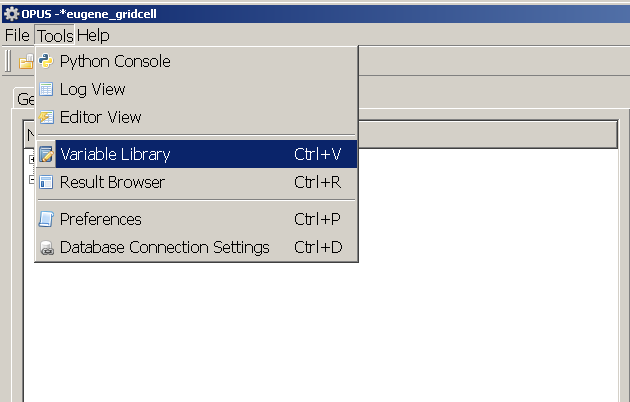
\includegraphics[scale=0.6]{part-gui/images/model-manager-variable-library-menu.png}
\end{center}
\caption{Variable Library Menu}
\label{fig:variable-library-menu}
\end{figure}

\begin{figure}[htp]
\begin{center}
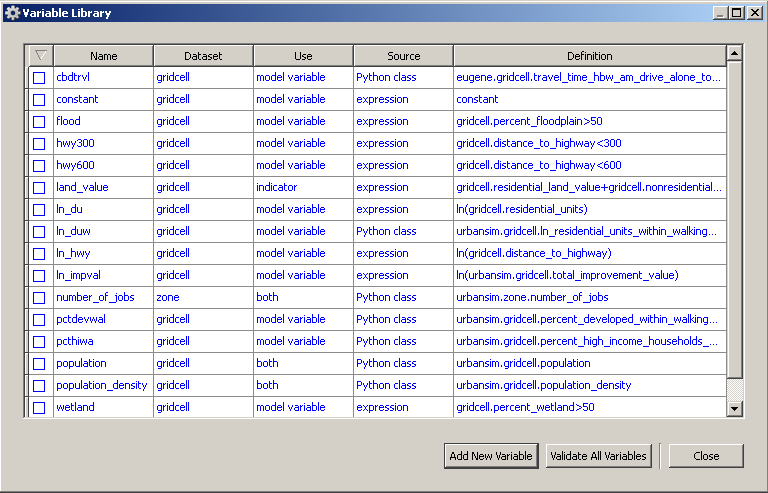
\includegraphics[scale=0.6]{part-gui/images/model-manager-variable-library-main.png}
\end{center}
\caption{Variable Library Main Window}
\label{fig:variable-library-main}
\end{figure}

Note the buttons at the bottom of this window to add new variables or validate all variables.  Adding a new variable is straightforward, using the GUI and the OPUS expression language, which provides a simple syntax for defining variables.  Notice examples of these in the variable library window, in the right-most column.  Expressions are simply functions of one or more primary attributes (think of these as columns in the input database) and possibly functions of other expressions as well.  For example, the expression for wetland is defined as gridcell.percent_wetland>50.  This defines the creation of a true/false, or boolean, variable that is interpreted as 1 if the gridcell has more than 50 percent coverage by wetland, 0 otherwise. Chapter \ref{chap:creating-variables} provides a more thorough introduction to the use of expressions and variables.

If you click on the add new variable button at the bottom of the variable library window, it opens a dialog box as shown in Figure \ref{fig:new-variable}.  The top entry is the name you want to use for the variable.  Let's say we want to create a new variable that is a log of population density.  We already have a population density variable defined by gridcell, so we can just take the log of this value.  Let's name the variable ln\_population\_density, leave the middle selection as \emph{expression}, and fill in a simple expression in the definition area: \emph{ln(gridcell.population_density)}.  Note that the dialog box provides two buttons to help you check your new variable.  The check syntax button tests whether the expression you have entered passes the Python and expression syntax checkers -- in other words, is it syntactically correct.  The second allows you to test whether if you apply this expression to your available data, it can successfully compute a result.  This is very helpful in determining whether you might have referred to a data element that is not present, or is otherwise not computable with your data.  In short, these two tools allow thoroughly testing whether the variables are in a state that can be computed on the available data.

\begin{figure}[htp]
\begin{center}
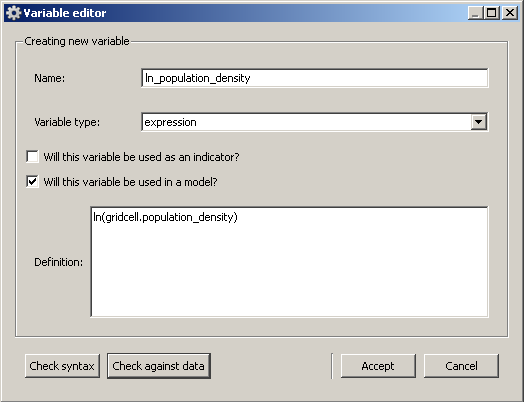
\includegraphics[scale=0.6]{part-gui/images/model-manager-variable-library-new-variable.png}
\end{center}
\caption{Adding a New Variable}
\label{fig:variable-library-new-variable}
\end{figure}
\chapter{The Menu Bar}

The main menu bar at the top of the OPUS GUI main window has three dropdown
menus: File, Tools, and Help.  The File menu includes the standard
operations of opening a project, saving a project, saving a project under a
new name, closing an OPUS Project, and finally exiting the OPUS GUI\@.  Help
offers an About option which produces a dialog box with information about
OPUS and a set of links to the UrbanSim website, online documentation, and
the GNU License.  The Tools menu provides access to several general tools,
described below.

Most of the items in the main menu bar are accessible from a secondary menu
bar just above the tabs on the left side of the OPUS GUI window.  Hovering
over each icon will yield a tooltip with the item's description.

\section{Tools}

The Tools menu, shown in figure \ref{fig:menu-bar-tools}, enables users to
adjust settings and preferences, as well as opening different tabs in the
right set of tabs.  The items labeled ``Python Console'', ``Log View'', ``Editor
View'', and ``Result Browser'' will each open new tabs on the right.  The
Result Browser is covered in greater detail in section
\ref{sec:interactive-result-exploration}.  The items labeled ``Variable
Library'', ``Preferences'', and ``Database Connection Settings'' each open a
popup when clicked.  The Variable Library is further discussed in section
\ref{chap:variable-library}.

\begin{figure}[htp]
\begin{center}
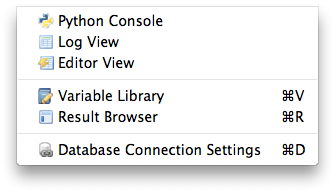
\includegraphics[scale=0.4]{part-gui/images/menu-bar-tools.png}
\end{center}
\caption{Tools Menu}
\label{fig:menu-bar-tools}
\end{figure}


\section{Preferences}

The Preferences dialog box changes some user interface related options in
the OPUS UI.  The dialog box is split into two sections, font preferences
and previous project preferences.  The font preferences section allows
users to adjust font sizes specific to different areas of the GUI.  The
previous project preferences section contains a checkbox allowing users to
open the most recently opened project each time OPUS GUI is started, this
is turned off by default.  Changes to the user preferences take effect as
soon as either the ``Apply'' or ``OK'' buttons are clicked.

\section{Database Server Connections}\label{sec:database-server-connections}

Database connections can be configured in the Database Server Connections
dialog launched from the Tools menu.  The Database Server Connections
dialog, pictured in Figure \ref{fig:menu-bar-database-connections}, holds
connection information for four database servers.  Each connection is used
for a specific purpose.  While there are four different connections that
must be configured, each may be configured to use the same host.  Every
connection requires a protocol, host name, user name, and password to be
entered.  Editing the protocol field produces a drop down of database
protocols that UrbanSim is able to use.  If a server has been setup for
UrbanSim's use choose the protocol that corresponds to the type of SQL
server being used.  If no SQL server is setup for a particular use, SQLite
may be used.  SQLite will create a local flat-file database instead of a
remote server.  UrbanSim currently supports MySQL, Microsoft SQL Server,
Postgres, and SQLite.

The Database Connection Settings are saved when the Accept Changes button
is pressed, ensuring that all future database connections will be made
using the new settings.  Database connections that are still in use while
the database connection settings are being edited will not be changed until
the connection is reestablished, for this reason it may be necessary to
reopen any open project after changing the database connection settings.

\begin{figure}[htp]
\begin{center}
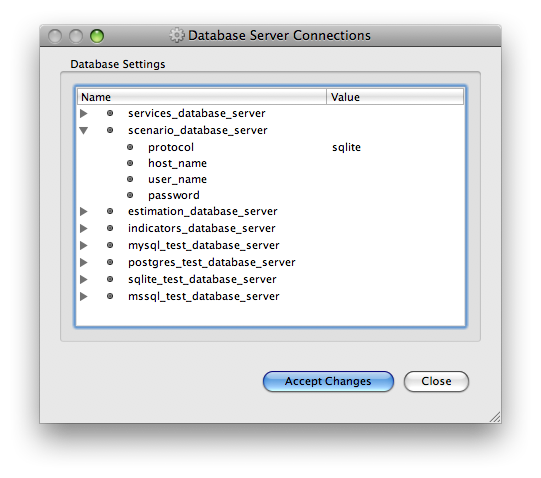
\includegraphics[scale=0.6]{part-gui/images/menu-bar-database-connections.png}
\end{center}
\caption{Database Connections}
\label{fig:menu-bar-database-connections}
\end{figure}

\chapter{General}

\chapter{The Data Manager}
The Data Manager\index{Data Manager} has two primary purposes, each reflected in the sub-tabs.  One tab, the Opus Data 
tab\index{Opus Data tab}, is for browsing, viewing, and exporting data from the Opus data cache.  
The other tab, the Tools tab\index{Tools tab}, is a place for storing and executing various tools provided by the Opus community or tools you have written.

\section{Opus Data Tab}

The Opus Data tab is a file browser that defaults to the folder in which
your project creates data.  This folder name is composed from the default 
location for the Opus files, followed by \file{data}, followed by the project
name.  The project name for the \file{eugene_gridcell_default.xml} project is
``eugene\_gridcell.'' (This is given in the ``project\_name'' element in the xml.)
Thus, if you installed to
\file{c:/opus}, and you are opening the Eugene sample project at
\file{c:/opus/project_configs/eugene_gridcell_default.xml}, the data folder
for this project is \file{c:/opus/data/eugene_gridcell}.  That is the
folder that this view starts at.  Any subfolders and files are displayed in
the tree view.  See Figure \ref{fig:opusdatatab}.

\begin{figure}[htp]
\begin{center}
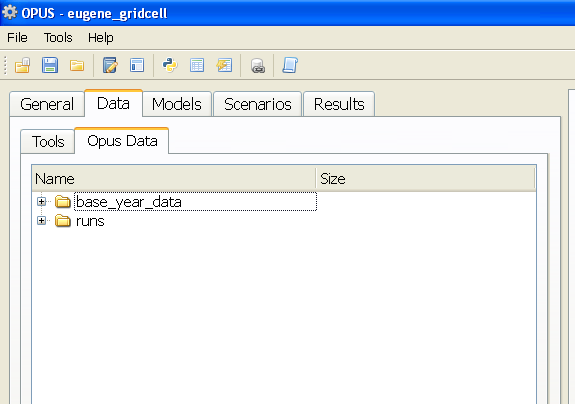
\includegraphics[scale=0.6]{part-gui/images/data-manager-opus-data-tab.png}
\end{center}
\caption{The Opus Data Tab}
\label{fig:opusdatatab}
\end{figure}

There could be any number of subfolders here, but by default you will find
a \file{base_year_data} folder\index{base\_year\_data}, and a \file{runs} folder\index{runs folder}.  The
base_year_data folder will normally contain an Opus \file{database} folder.
An Opus database folder\index{Opus database folder} is any folder containing Opus \file{datasets}.
Often Opus database folders are titled with a year, such as 2000.  Opus
datasets are folders containing Opus `data arrays.'  Opus datasets are
equivalent to the tables in a database.  Opus data arrays are equivalent to
the columns in a table, and are simply numpy arrays that have been written
to disk in a binary format.  See Figure \ref{fig:db-dataset-array}.

\begin{figure}[htp]
\begin{center}
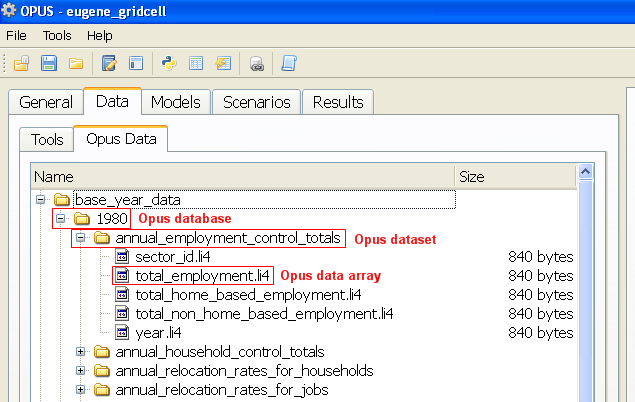
\includegraphics[scale=0.6]{part-gui/images/data-manager-opus-data-tab-db-dataset-array.png}
\end{center}
\caption{Opus databases, datasets, and arrays}
\label{fig:db-dataset-array}
\end{figure}

The Opus data arrays are referred to throughout the documentation as
`primary attributes.'  Primary attributes are the actual data columns in a
dataset.  Computed attributes are attributes computed from primary
attributes via expressions.  For instance, if a parcels dataset contained
the primary attributes population and area, a computed attribute called
population_density could be computed by using the expression
\variable{population_density = population/area}.  Once this expression is
entered and stored in your project in the Variable Library, it can be used
in a model and would be computed as needed.  See Chapter~\ref{chapter:expressions} 
for more details on expressions.

\subsection{Viewing and Browsing an Opus Data table}
To view and browse the contents of an Opus dataset, right-click a data table, then select 'View Dataset'.  This will bring up a new tab on the right-hand side of the Opus GUI window that will display some summary statistics about the dataset, and a table view of the raw data that can be browsed and sorted by clicking the column name.  See Figure \ref{view-and-browse} for an example of browsing a data table.

\begin{figure}[htp]
\begin{center}
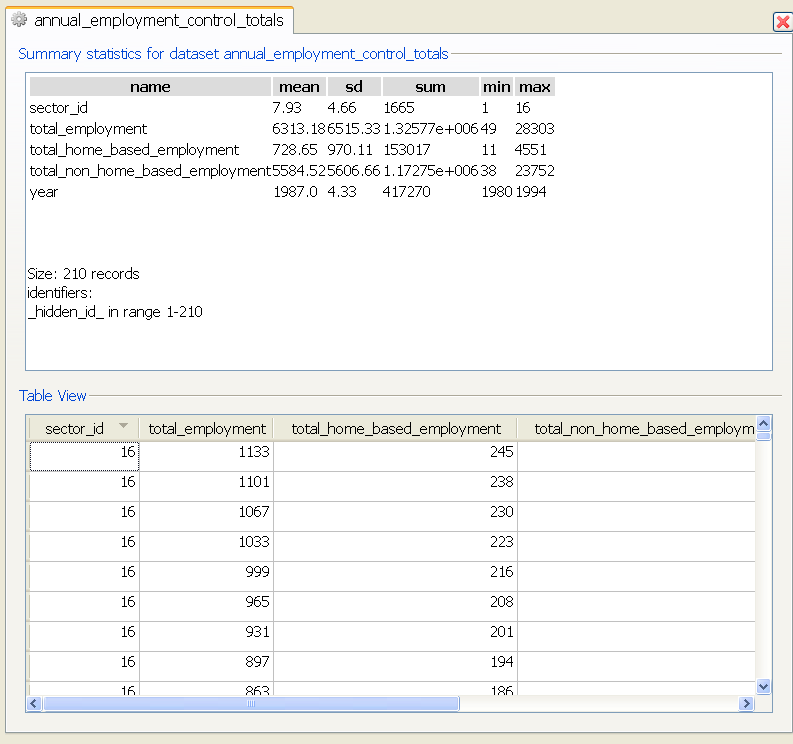
\includegraphics[scale=0.5]{part-gui/images/data-manager-opus-data-tab-view-dataset-tab.png}
\end{center}
\caption{Viewing and browsing an Opus dataset}
\label{view-and-browse}
\end{figure}

\subsection{Exporting an Opus Data table}
An Opus dataset can be exported to another format for use in other applications.  By default there are 3 options: ESRI, SQL, and CSV.  To export a dataset, right-click a dataset, choose 'Export Opus dataset to,' then click your choice.  See Figure \ref{exporting} for the right-click menu.  You will then see a pop-up window with the respective export tool with the parameters partially filled in based on which dataset you clicked.  These are the same tools that you will find in the Tools tab of the Data Manager.  For more information on the individual tools see the help tab on each tool.

\begin{figure}[htp]
\begin{center}
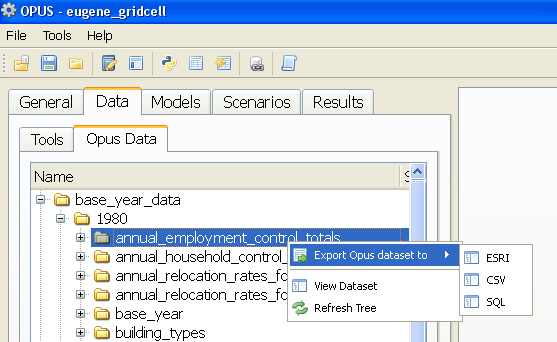
\includegraphics[scale=0.8]{part-gui/images/data-manager-opus-data-tab-export-dataset.png}
\end{center}
\caption{Exporting an Opus dataset}
\label{exporting}
\end{figure}

\section{Tools Tab}
The Tools tab\index{Tools tab} is an area to collect and execute tools and batches of tools provided with the interface, or it can be extended with tools that you  write.  A Tool is simply any script that is written in Python and executed by the interface.

\subsection{Tool Library}
The Tool Library\index{Tool library} is a place to collect and organize your tools.  Tools can also be executed directly from the library in a 'one-off' manner, meaning that you can supply parameters to the tool and execute it without storing those parameters for future use.  To execute a tool from the library, simply right-click it and choose 'Execute Tool...', see Figure \ref{execute-tool}.  This will pop-up a window in which you can supply parameters to the tool then execute it.

\begin{figure}[htp]
\begin{center}
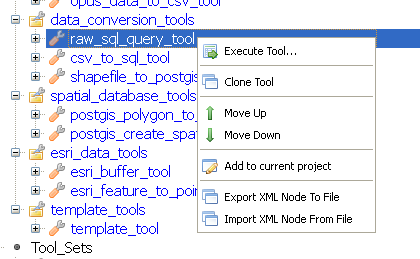
\includegraphics[scale=0.8]{part-gui/images/data-manager-opus-tools-tab-execute-tool.png}
\end{center}
\caption{Executing a tool}
\label{execute-tool}
\end{figure}

\subsubsection{Extending the Tool Library}
New tools can be written and added to the tool library fairly easily.  The best way to explain this is to use an example.  A 'template_tool' has been provided so you can see how it works.  Feel free to execute the template_tool, it just implements a simple loop and prints the results to the tool's log window.  The template_tool's code and associated XML display everything that is needed to add a tool to the interface.  See the code in the source code tree at /opus_gui/data_manager/run/tools/template_tool.py.  A tool also needs XML configuration data in an Opus project.  To view the XML configuration data for the template_tool, open urbansim.xml in an XML editor from the source code tree at /urbansim/configs and search for template_tool.

At the time of this writing new tools must be placed in the source tree at /opus_gui/data_manager/run/tools in order to run correctly.  There are plans to create an additional 'user tools' folder where tools could also be placed.  Also, at this moment, the XML must be hand written to ensure that the tools show up properly in the interface and execute correctly.  There are some right-click functions in the Tool Library to assist with the XML editing (to add a new tool, create parameters for it, etc.) but these functions are in a beta state.

Once a new tool and its associated XML is written properly, the Tool Library will display the tool and dynamically populate the pop-up dialog box with the proper parameters based on the XML configuration.  The tools are quite flexible.  Although the initial tool must be written using Python, there is no limit placed upon what one can do.  For starters, there are tools provided in the interface that make OS calls to external executables (e.g. ogr2ogr.exe), databases, and myriad other libraries to accomplish various tasks (e.g. ESRI geoprocessing).  Feel free to browse the source code for any provided tool along with the XML configuration to see some possibilities.

\subsection{Tool Sets}
Tool Sets are simply collections of tools from the Tool Library with parameters stored so they can be executed repeatedly or in order in a batch manner.  Tool Sets can contain any number of tools from the Library.  A new Tool Set can be created by right-clicking Tool_Sets and choosing 'Add new tool set.'  This adds a new Tool Set to the bottom of the list.  It can be renamed by double-clicking it and typing in a name, taking care to not use spaces or a leading integer as these are invalid in XML nodes.  Once you have a new Tool Set, tools from the Library can be added to it by right-clicking a Tool Set and choosing 'Add Tool to Tool set.'  See Figure \ref{addtool} for an example of what this looks like.

\begin{figure}[htp]
\begin{center}
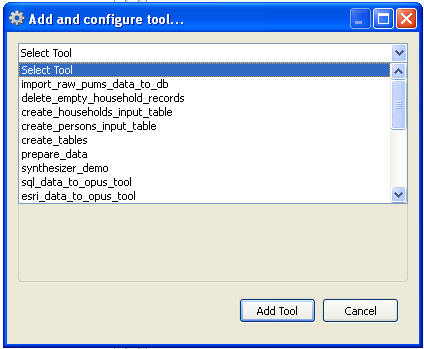
\includegraphics[scale=0.8]{part-gui/images/data-manager-opus-tools-tab-add-tool-to-tool-set.png}
\end{center}
\caption{Adding a tool to a Tool Set}
\label{addtool}
\end{figure}

From this window, choose a tool from the drop down menu, fill in the parameters, then click 'Add Tool.'  The tool is added to the Tool Set and the parameters you entered are stored in the project XML file.  This configured tool can now be executed by itself with those parameters, or executed as part of a batch in the Tool Set.  Tools in a Tool Set can be re-ordered by right-clicking them and choosing to move them up or down, and all of the tools can be executed in the order they appear by right-clicking a Tool Set and choosing 'Execute Tool Set'.

\chapter{The Models Manager}

The model manager tab\index{Model Manager tab} in the GUI provides the functionality to create models of various types, configure them, specify the variables to use in them, and then estimate their parameters if they have a form that needs to be estimated -- such as regression models or discrete choice models.  A more thorough description of the types of models that can be implemented in OPUS is provided in Chapter \ref{chap:creating-models}.

\begin{figure}[htp]
\begin{center}
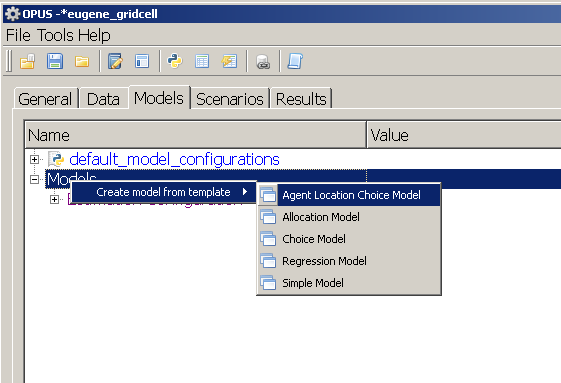
\includegraphics[scale=0.6]{part-gui/images/model-manager-create-model-from-template.png}
\end{center}
\caption{Creating a New Model from a Template}
\label{fig:create-model}
\end{figure}

\section{Creating an Allocation Model}

To demonstrate the process of creating models\index{creating an Allocation Model} in the GUI, let's begin with a simple allocation model, which does not have any parameters to estimate and represents a straightforward model to configure.  Say we want to create a model that allocates home-based jobs to zones, and lack sufficient data to specify a choice model or regression model for this purpose.  Home-based jobs are those jobs that are located in properties that are residential in character.  Assume that we have no behavioral information about this problem, other than the insight that home-based jobs are... home-based.  So we can infer that we should probably allocate these jobs to places that have housing (or households).  In allocating these jobs to zones (traffic analysis zones used in the travel model), we can count how many residential units are in each zone, and use this as the weight to allocate the total home-based jobs to zones.  That is, we want to proportionately allocate home-based jobs to zones, weighted by the number of residential units in the zone.  This is equivalent to saying that we want each residential unit to have an equal probability of receiving a home-based job (assuming that we do not have any information to suggest which residential units would be more likely than others to receive such a job).

The next consideration is the capacity of zones to absorb home-based jobs.  One simplifying assumption we could make is that there is a maximum of one home-based job per residential unit in a zone.  On average, our aggregate information suggests that most residential units do not have a home-based job, so this assumtion should not be constraining.

We now have all the information we need to specify a model for home-based jobs.  We will name the model allocate\_home\_based\_jobs, to be descriptive.  The table below contains the \emph{arguments} we will need to use in creating this model in the GUI.

\begin{table}[htp]
\caption{Creating an Allocate Home Based Jobs Model}
\label{tab:allocation-model}
\begin{center}
\begin{tabular}{ p{1.5in}  p{4.4in}  }
\toprule[1.5pt]
Configuration Entry & Value \\
\midrule
Model Name & allocate\_home\_based\_jobs\_model \\
Dataset & zone \\
Outcome Attribute & home\_based\_jobs \\
Weight Attribute & zone.aggregate(building.residential\_units) \\
Control Totals & annual\_employment\_control\_totals \\
Year Attribute & year \\
Capacity Attribute & zone.aggregate(building.residential\_units) \\
\bottomrule
\end{tabular}
\end{center}
\end{table}

The create new model dialog box (Figure {fig:create-model}) contains several kinds of model templates we could create a model from. One of these is Allocation Model. The capacity to create new allocation models, such as this, is now available in the Opus GUI. Select Allocation Model from the list, and a new dialog box appears, with several fields to fill in.  Fill in the fields with the contents from Table \ref{tab:allocation-model}, and save it.  Once this is done, it will appear in the list of models under the Models section of the Model Manager tab.  It is now a fully enabled model, and can be included in a simulation run.

It should go without saying (but doesn't), that creating models through the GUI, with a few mouse clicks and filling in a few fields in a dialog box, is much, much easier than it has been in the past. One does not need to be an expert software developer in order to create and use interesting and fully functional models in OPUS.


\begin{figure}[htp]
\begin{center}
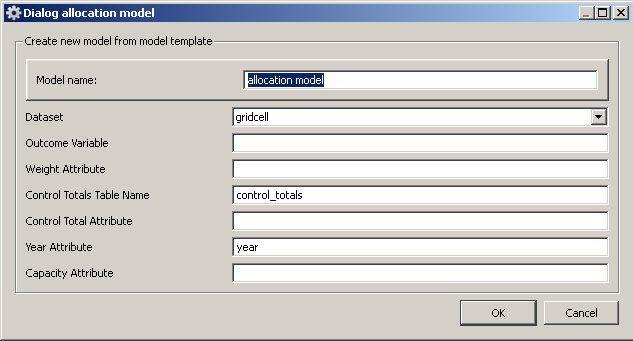
\includegraphics[scale=0.6]{part-gui/images/model-manager-create-allocation-model-from-template.png}
\end{center}
\caption{Creating a New Allocation Model from a Template\index{creating an Allocation Model}}
\label{fig:create-allocation-model}
\end{figure}

\section{Creating a Regression Model}

Regression models\index{creating a Regression model} are also simple to create and specify in the Opus GUI, and can be estimated and simulated within the graphical interface.    Assume we want to create a model that predicts population density, using the population per gridcell as the dependent variable and other attributes we can observe about gridcells as independent (predictor) variables.  Note that this is not a very useful model in this context since we actually have a household location choice model to assign households to gridcells -- so this model is for demonstration purposes only.

To create this model in the Opus GUI, right-click again on Models, and select in this case Regression Model to generate a new dialog box for this model template, as shown in Figure \ref{fig:create-regression-model}.  We just need to provide three arguments in the dialog box - a name to assign to the new model (we will use population\_density\_model), a dataset to contain the dependent variable (gridcell), and the name of the dependent variable (population\_density) - which should exist in the base year, or be an expression to compute it from other attributes already in the data.


\begin{figure}[htp]
\begin{center}
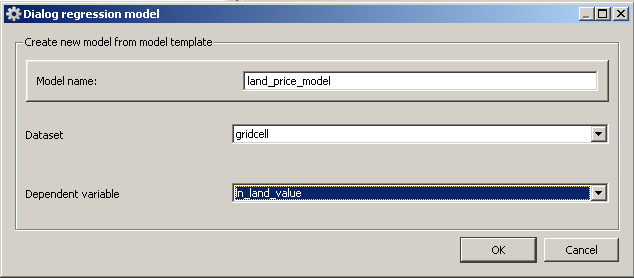
\includegraphics[scale=0.6]{part-gui/images/model-manager-create-regression-model-from-template.png}
\end{center}
\caption{Creating a New Regression Model from a Template\index{creating a Regression model}}
\label{fig:create-regression-model}
\end{figure}

Once the values have been assigned to the configuration of the new model, and you click OK on the dialog box, the model is added to the list of models under Models.  If you expand this node by clicking on the plus sign to the left of the new land price model entry, you will see that it contains a specification and a structure node.  Expand the specification node, and you will find some additional detail, including a reference to submodels, and a variables entry.  We will ignore submodels for now -- it is a means of specifying that you would like to specify the model differently for different subsets of the data.  For now we will just apply a single specification to all the data, to keep this a bit simpler.  We can now move to the task of specifying and estimating this model. 

Right-click on the variables node, and click on Select Variables, as shown in Figure \ref{fig:specify-regression-1}.  At this point a window should appear as shown in Figure \ref{fig:specify-regression-2} that is essentially the same as the variables library window you encountered earlier.  There is a column of check-boxes at the left hand side of the window which you can use to identify the variables you want to include as independent variables, or predictive variables, for this model.  The button at the bottom allows you to accept the selection, which then updates the list of variables in the model specification.  Try adding a constant term, since this is a regression and we need an intercept, or a base value.  Also add a variable like population density.  Now accept the selections.


\begin{figure}[htp]
\begin{center}
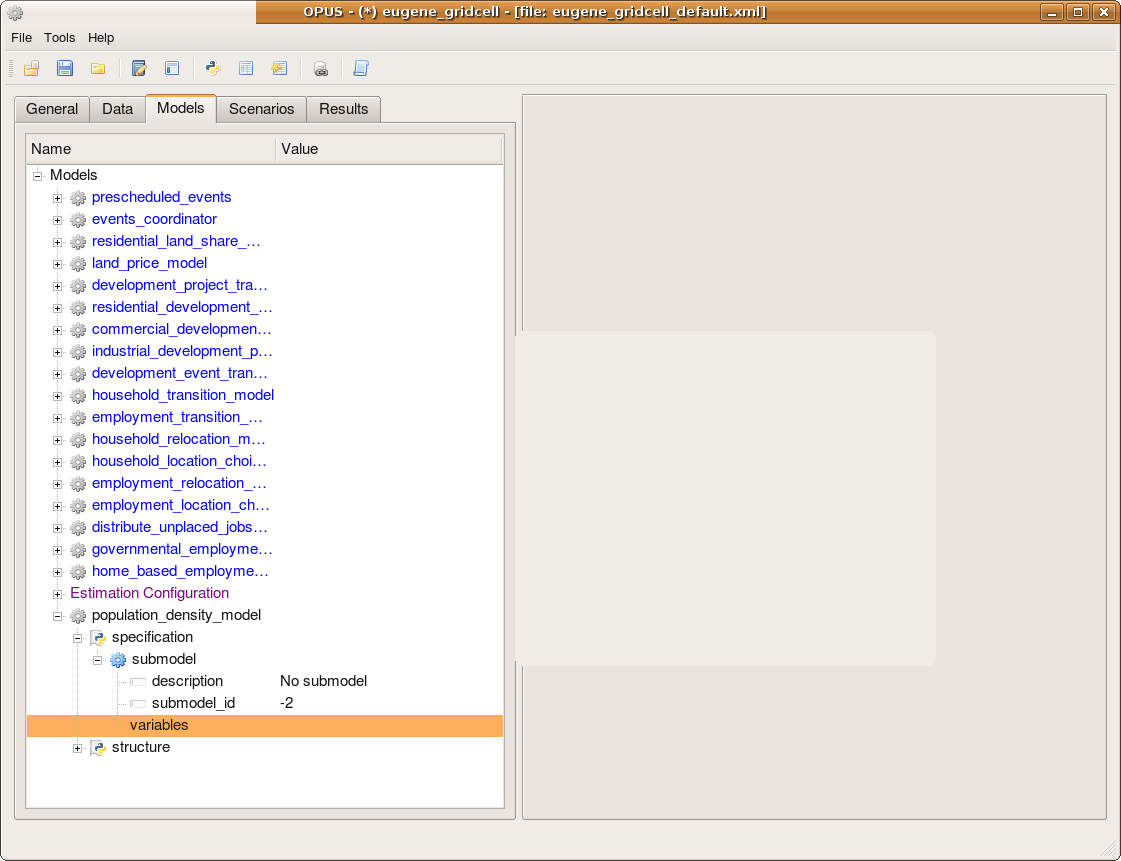
\includegraphics[scale=0.4]{part-gui/images/model-manager-specify-regression-model-1.png}
\end{center}
\caption{Specify the New Population Density Model}
\label{fig:specify-regression-1}
\end{figure}

\begin{figure}[htp]
\begin{center}
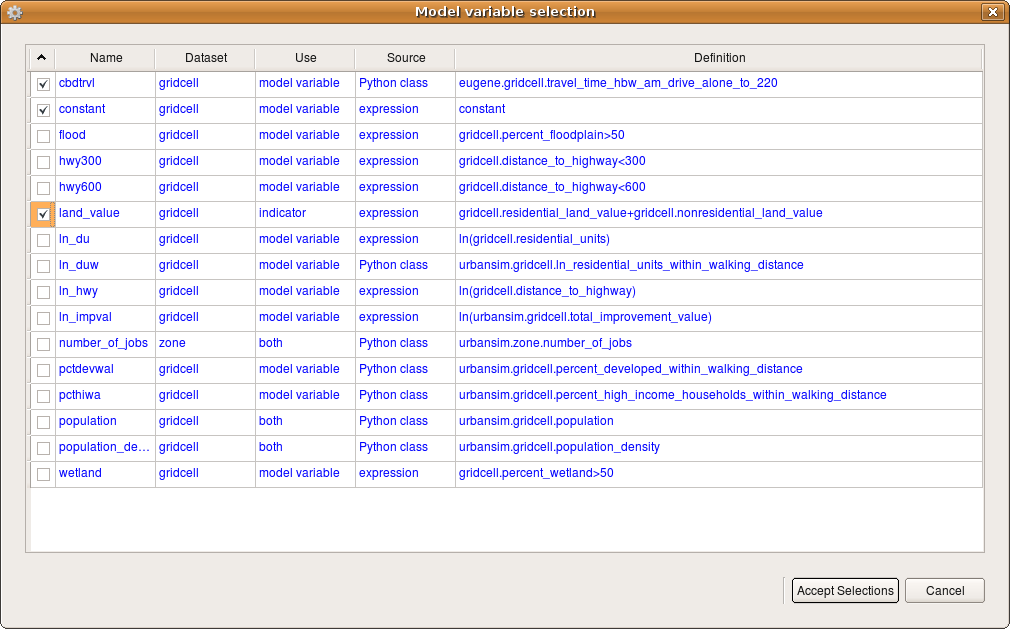
\includegraphics[scale=0.4]{part-gui/images/model-manager-specify-regression-model-2.png}
\end{center}
\caption{Select Variables for Specification}
\label{fig:specify-regression-2}
\end{figure}


Once the model specification has been entered, we can estimate the model parameters using Ordinary Least Squares by right-clicking on the population density model and selecting Run Estimation, as shown in Figure \ref{fig:specify-regression-3}. Once this has been clicked, a new tab appears on the right hand side of the main window, to interact with the model estimation.  Click on the start estimation button, and within a few seconds you should see the estimation results appear in this tab, as shown in Figure \ref{fig:specify-regression-4}.

\begin{figure}[htp]
\begin{center}
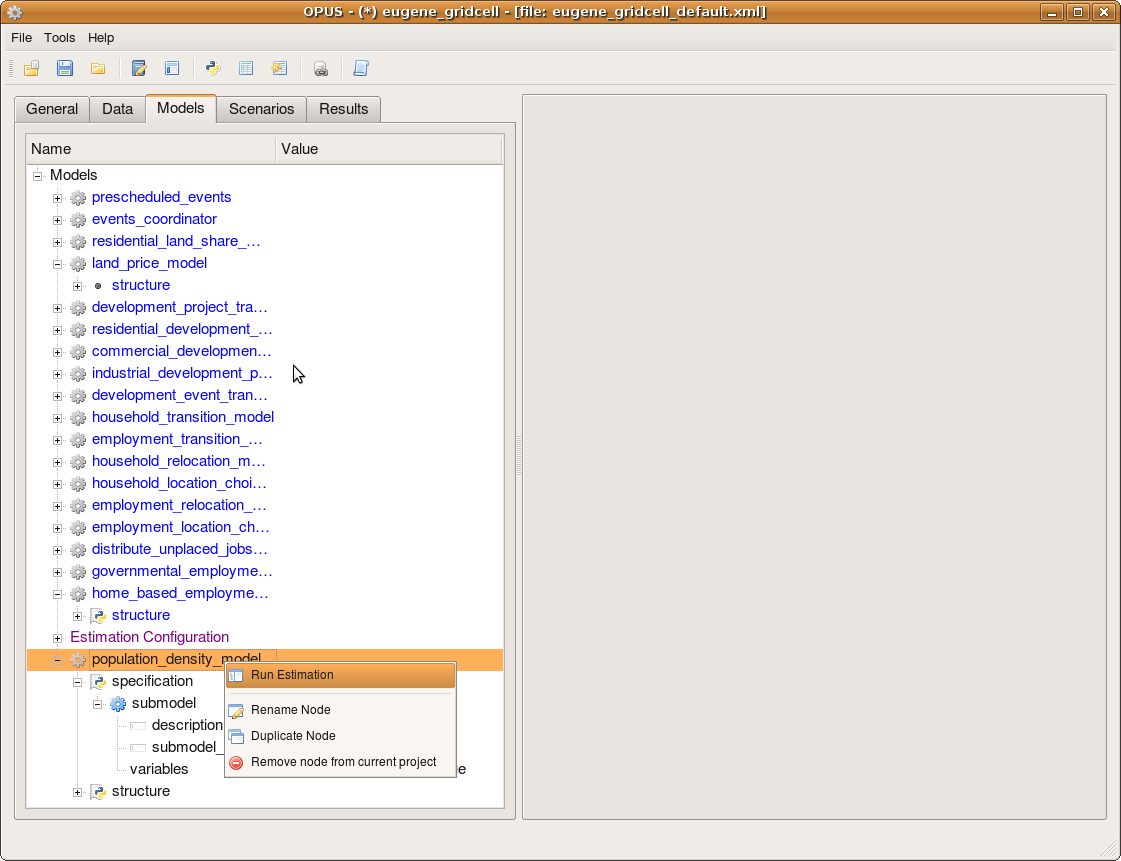
\includegraphics[scale=0.4]{part-gui/images/model-manager-specify-regression-model-3.png}
\end{center}
\caption{Estimate the New Population Density Model}
\label{fig:specify-regression-3}
\end{figure}

\begin{figure}[htp]
\begin{center}
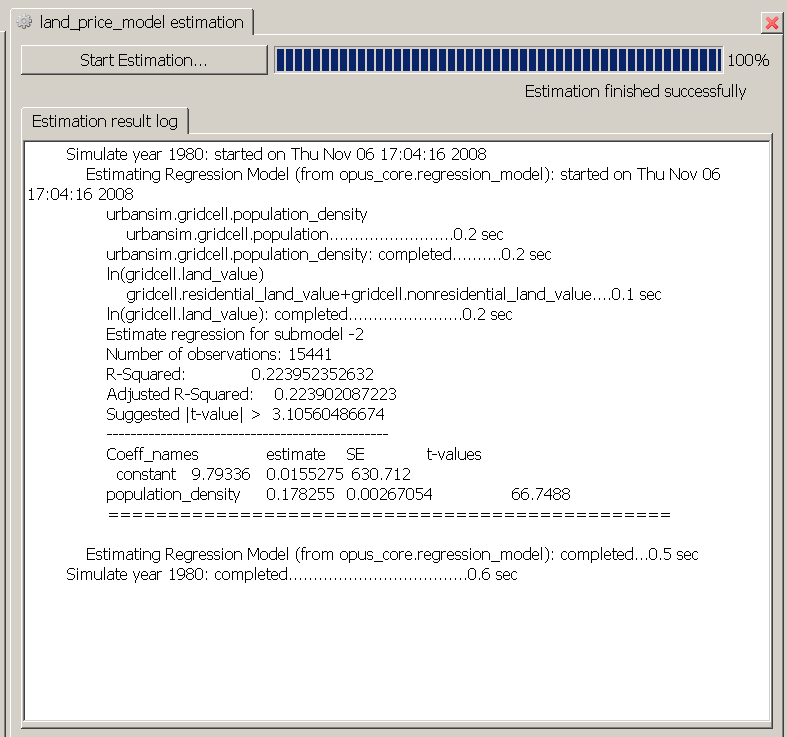
\includegraphics[scale=0.4]{part-gui/images/model-manager-specify-regression-model-4.png}
\end{center}
\caption{Estimation Results}
\label{fig:specify-regression-4}
\end{figure}

We can see from the results that the constant and travel time to the CBD, and also land value were quite statistically significant, and that they explain around 28 percent of the variation in population density in Eugene.  Clearly this is a toy model, but adding other variables in this way can increase the explanatory power to a quite useful level, and as you can see modifying the specification and estimating the model is not difficult to do.

One other note at this point is that the specification and estimation results are automatically stored, if you request this, as shown in Figure  \ref{fig:save-estimation}.  Once the estimation is done, then, the model is ready to use in a simulation, or predictive mode.  More on this in the Scenario Manager section.

\begin{figure}[htp]
\begin{center}
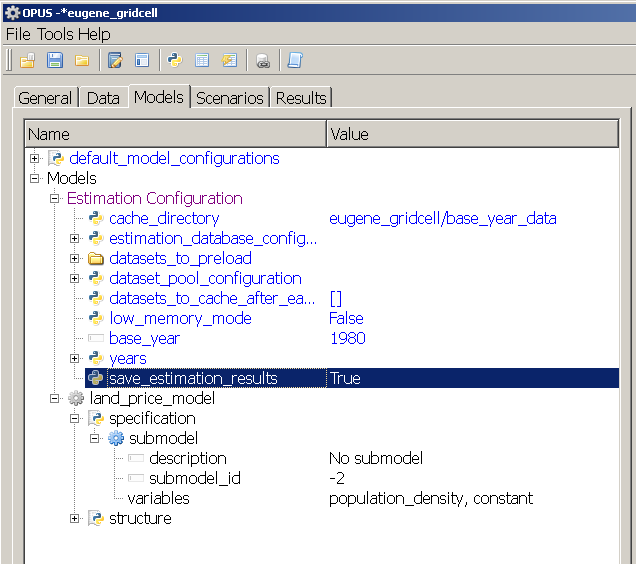
\includegraphics[scale=0.6]{part-gui/images/model-manager-save-estimation.png}
\end{center}
\caption{Save Estimation Results Flag}
\label{fig:save-estimation}
\end{figure}


%\section{Creating a Choice Model}
% Replace this later, after further testing and cleanup
%The next type of model we will create is a choice model.  This is a very common modeling application, and is used widely.  Our example for this demonstration is a model of housing type choice, which for purposes of keeping the example simple, we reduce to two alternatives: single-family housing type, or other.  It is likely that households choosing to live in single-family housing may make different trade-offs in other choices, such as travel, and car ownership.  By reducing the model to two outcomes, we create a binary choice model specification.  We always need to use one alternative as a base of comparison in choice models, so for this model we will use the other housing type as the base of comparison.  

%Below are the configuration settings for creating a choice model of housing type.  In order to create this model for estimation purposes, we will exclude the few households that are in non-residential property types, and only keep those in multi-family, condominium, and single-family housing.  These are reflected by building type id values of 4, 12, and 19, respectively, in the seattle parcel data.  Filtering the data to include only these three values can be done with the numpy logical\_or command, but since it takes only two arguments, we need to create a nested comparison, as shown below.  Since there are three housing types represented in this data, and we want to create a binary choice outcome for simplicity, it is necessary to create a dependent variable that is 2 if the household occupies a single family house, and 1 otherwise.  In this example, since we will use the entire household table, we draw a small sample of 5\% of the agents to use in estimating the model.

%\begin{table}[htp]
%\caption{Creating a Housing Type Choice Model}
%\label{tab:housing-type-choice-model}
%\begin{center}
%\begin{tabular}{ p{1.2in}  p{1.2in} p{3.2in}  }
%\toprule[1.5pt]
%Configuration Entry & Node & Value \\
%\midrule
%Model Name & & housing\_type\_choice\_model \\
%Choice Set & Init & [1, 2] \\
%Choice Attribute & Init & single\_family=(household.disaggregate\\ & & (building.building\_type\_id)==19)+1 \\
%Estimation Size Agents & Init.Estimation Config & 0.05 \\
%Agent Set & Run, Prepare for Run, Estimate, Prepare for Estimate & household \\
%Agent Filter & Prepare for Run & numpy.logical\_or(numpy.logical\_or(household.\\ & & %disaggregate(building.building\_type\_id)==4,household. \\ & & disaggregate(building.building\_type\_id)==12),household.\\ & & %disaggregate(building.building\_type\_id)==19) \\
%Specification Table & Prepare for Run & housing\_type\_choice\_model\_specifications \\
%Coefficients Table & Prepare for Run, Prepare for Estimate & housing\_type\_choice\_model\_coefficients \\
%\bottomrule
%\end{tabular}
%\end{center}
%\end{table}

%Figure \ref{fig:configure-choice-model} shows the housing type choice model configuration in progress.  For a binary choice model such as this, the specification of the model is quite similar to the specification of the regression model, but there are some subtle differences.  The most important one is that, as this model is implemented in Opus now, it requires at least one variable in each equation - that is - per alternative.  We typically assign the constant to alternative 1, and all other variables to alternative 2.  In a future revision of the code, the base alternative will not take any variables (this is the more standard implementation).  Figure \ref{fig:choice-model-specification} shows the initial specification of the housing type choice model, with a constant for the other housing types, and income and has\_children included in the utility specification for the single family housing alternative. 

%Once the model is specified, it needs to be added to the list of models to estimate, and selected as the model to estimate, as was the case in the preceding regression model example.  Once the model has been added and the project saved, the model can be estimated with the normal right-click option on the models to estimate node.  The results are shown in Figure \ref{fig:choice-model-estimation}.

%\begin{figure}[htp]
%\begin{center}
%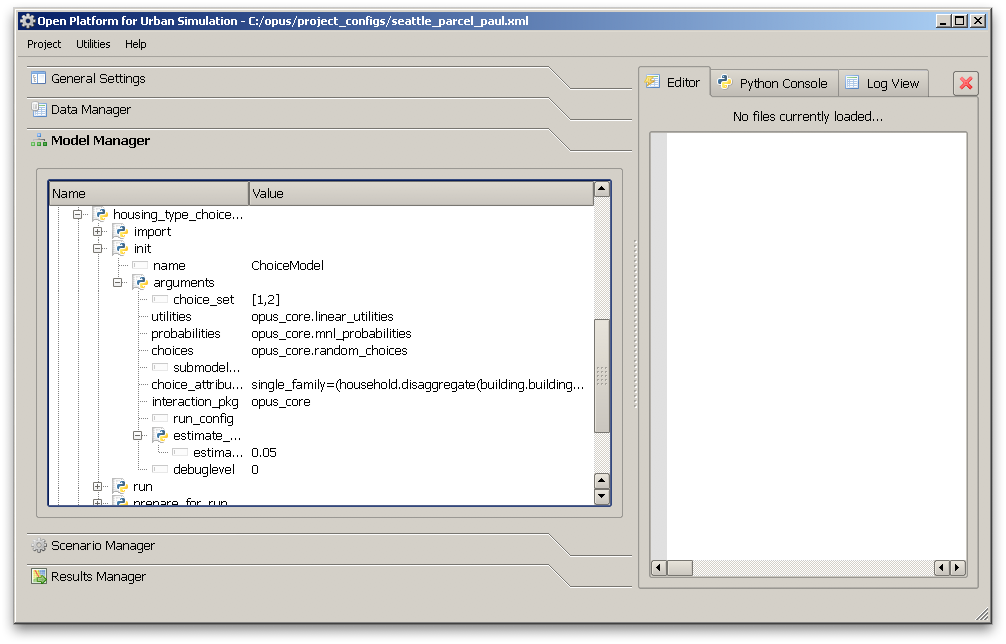
\includegraphics[scale=0.35]{graphics/configure-choice-model.png}
%\end{center}
%\caption{Configuring the Housing Type Choice Model}
%\label{fig:configure-choice-model}
%\end{figure}

%\begin{figure}[htp]
%\begin{center}
%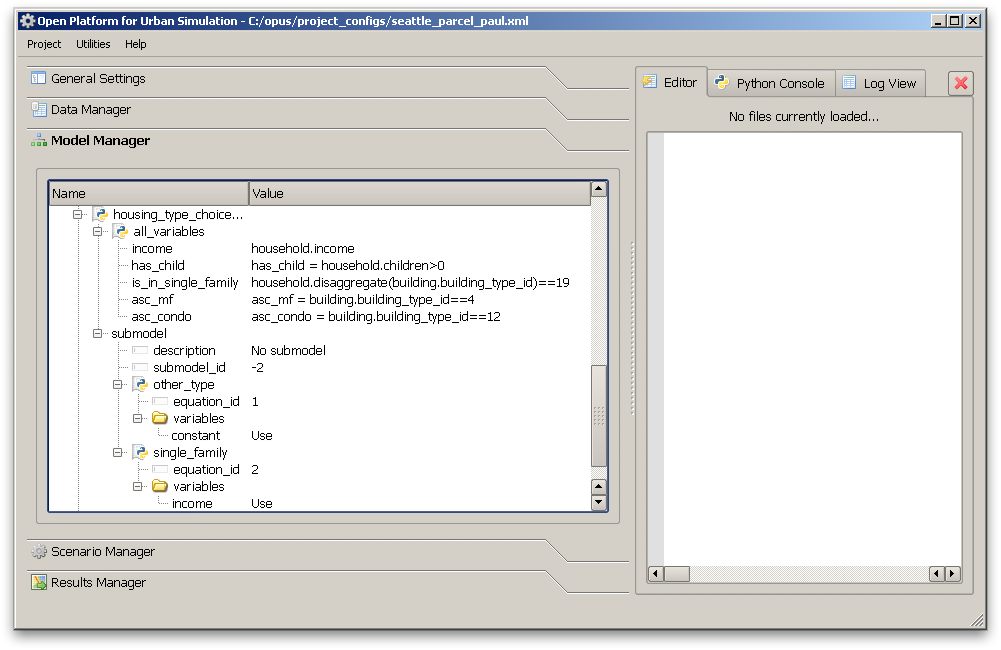
\includegraphics[scale=0.35]{graphics/choice-model-specification.png}
%\end{center}
%\caption{Specifying the Housing Type Choice Model}
%\label{fig:choice-model-specification}
%\end{figure}

%\begin{figure}[htp]
%\begin{center}
%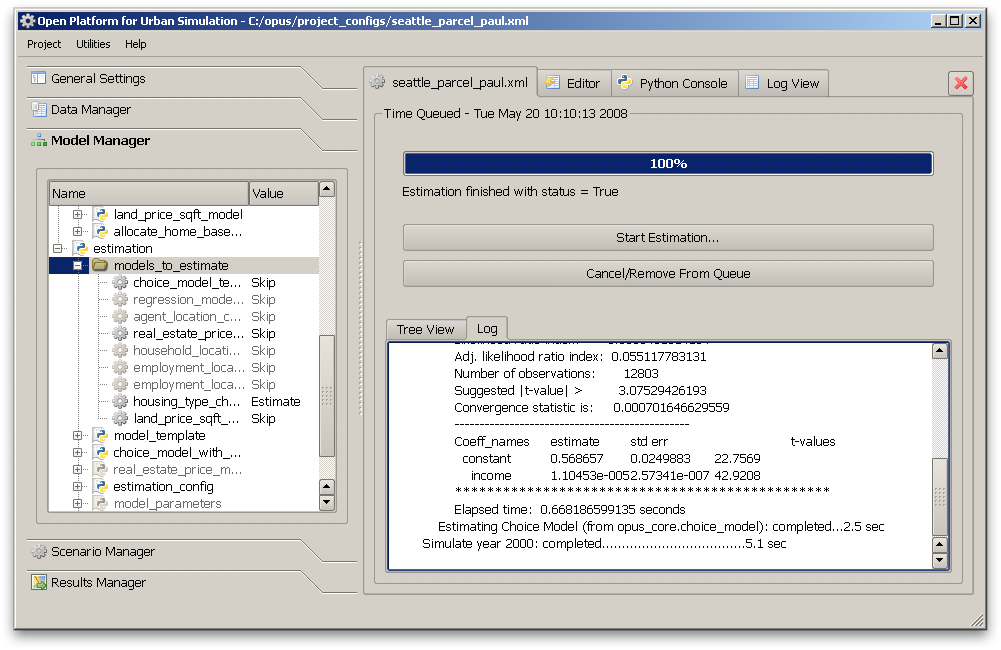
\includegraphics[scale=0.35]{graphics/choice-model-estimation.png}
%\end{center}
%\caption{Estimating the Housing Type Choice Model}
%\label{fig:choice-model-estimation}
%\end{figure}

\chapter{The Scenarios Manager}
\label{chap:scenarios-manager}

\section{Running a Simulation}
Once a project has been developed, including the data to be used in it, and the model system has been configured and the parameters for the models estimated, the next step is to create and run a scenario.  In the eugene\_gridcell project, a baseline scenario has already been created and is ready to run.  To run this scenario, in the Scenario Manager, right-click with the mouse on the Eugene-baseline entry and select \verb#Run this Scenario#.  At this point, a frame should appear in the right hand side of the Opus window, as shown in Figure \ref{fig:opus-start-run}.

\begin{figure}[htp]
\begin{center}
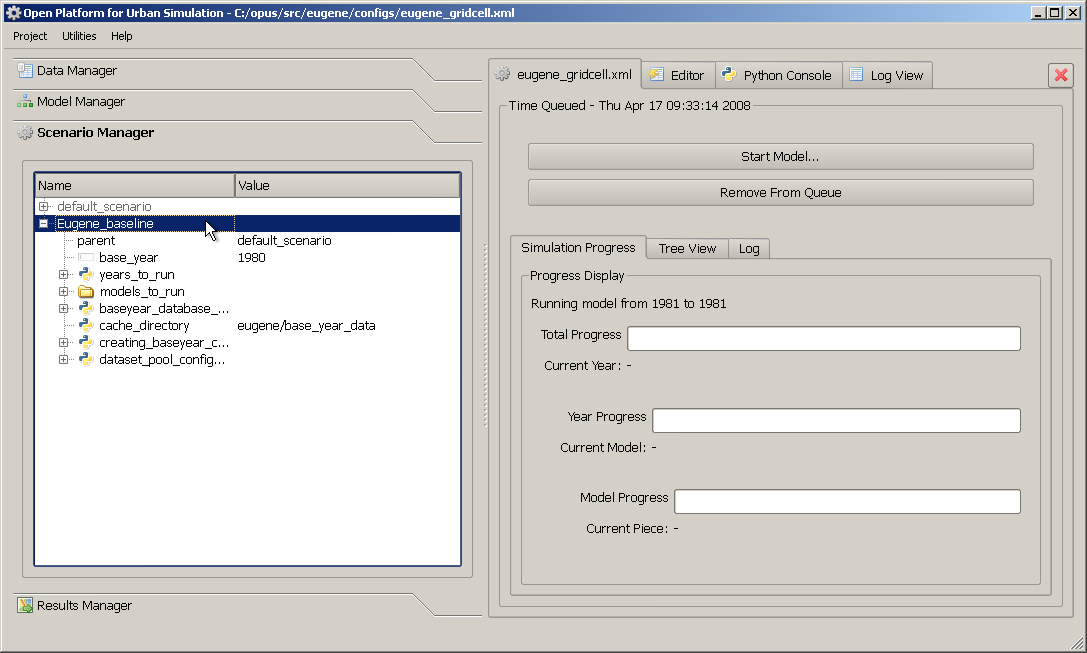
\includegraphics[scale=0.4]{graphics/opus-start-run.png}
\end{center}
\caption{Starting a Simulation on a Scenario.xml}
\label{fig:opus-start-run}
\end{figure}

The frame on the right contains an option to start the run and an
option to remove the run from the queue.  The latter will remove this
new frame so that it is no longer available to run.  Start the run with
the first button option, labelled \verb#Start Model#.  The window will
now update as the simulation proceeds, with progress bars and labels
being updated to show the changing state of the system, such as what
year the model is simulating, what model is running, and even what part
of a model is running.  Figure \ref{fig:opus-running} shows the updated
window in this state.  Note that the \verb#Start Model#  button label
has now changed to \verb#Pause Model#.  If this is pressed while the
model system is running, a request to pause the model is triggered, and
once the current model in the model system is finished, the system
pauses until you take further action, like resume, or remove from
queue.

\begin{figure}[htp]
\begin{center}
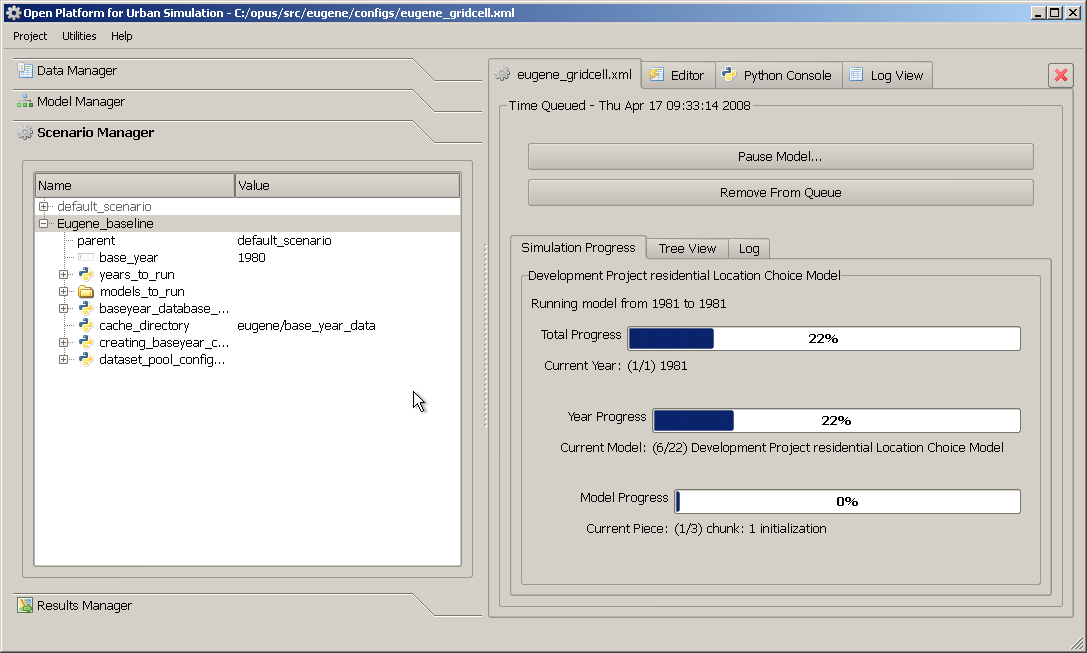
\includegraphics[scale=0.4]{graphics/opus-running.png}
\end{center}
\caption{Running a Simulation on a Scenario.xml}
\label{fig:opus-running}
\end{figure}


% \begin{figure}[htp]
% \begin{center}
% 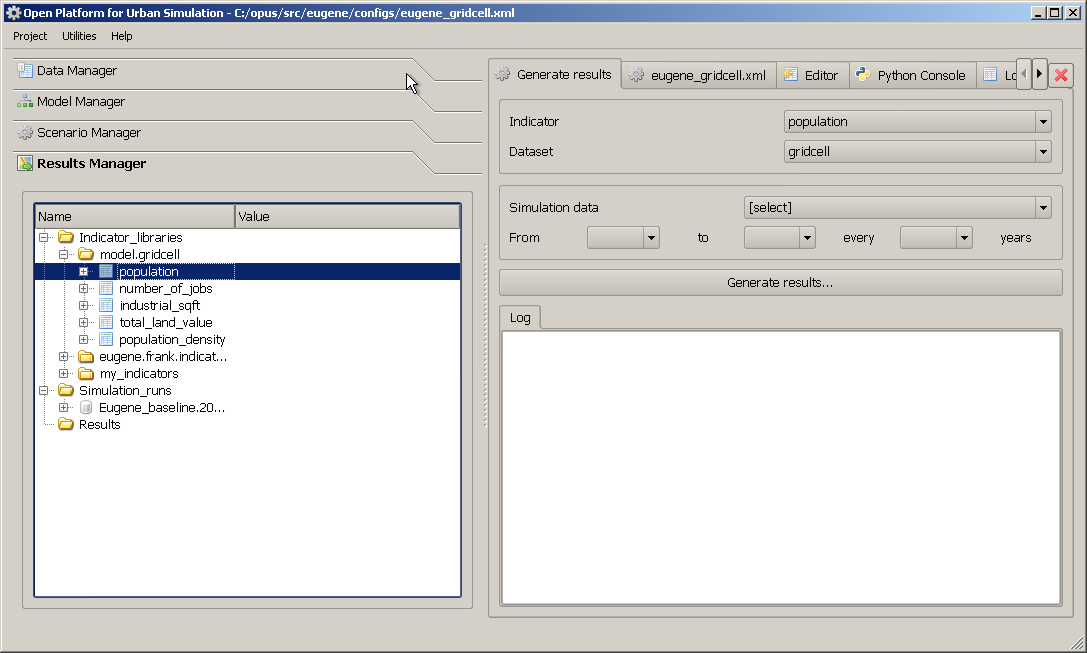
\includegraphics[scale=0.4]{graphics/opus-generate-indicator.png}
% \end{center}
% \caption{Generating an Indicator in the Results Manager}
% \label{fig:opus-generate-indicator}
% \end{figure}


\chapter{The Results Manager}

The Results Manager, corresponding to the Results tab of the GUI, has
two main responsibilities: to manage simulation runs for this project
and to allow the interrogation of these simulation results through
the use of \emph{indicators}. We explore both of these in this
chapter.

\section{Managing simulation runs}

[get run info]
[remove run and delete from harddrive]
[import run from disk]


\section{Interrogating results with Indicators}

Indicators are variables defined explicitly
for use as a meaningful measure. Like model variables, they can be
defined using the domain-specific programming language via the
``Variable Library'' item in the Tools menu. (XXX: forward pointer to
indicator chapter). An indicator can then be visualized as either a
map or as a table (the raw data) in a variety of formats. 

The GUI provides two ways to use indicators to understand what has
happened in your simulation:
\begin{enumerate}
  \item Interactive result exploration
  \item Batch indicator configuration and execution
\end{enumerate} 

\subsection{Interactive result exploration}

Often, it is desirable to explore your results in a lightweight
fashion in order to get a basic idea of what happened. You don't
necessarily want to go through the process of exporting results to a
GIS mapping tool in order to gain some intuition. 

The Opus GUI's \verb#Result Browser#, available from the \verb#tools#
menu, allows interactive exploration of simulation results. The Result
Browser presents a selectable list of available simulation runs, years
over which those simulations were run, and available indicators. You
can then configure an indicator visualization by selecting a simulation
run, a year, and an indicator. To compute and visualize the configured
indicator, simply press the \verb#generate results# button. The
indicator will then be computed for the year of the selected simulation
run. After it is computed, a tab should appear at the bottom of the
window with the name of the indicator and provide the ability to
visualize the results as a table or map (using the MatplotLib Python
module). See the inset tutorial XXX to try out the \verb#Result
Browser#.

\fbox{
\begin{minipage}{.5\linewidth}
\begin{enumerate}
  \item \cmd{Open the Results Browser from the Tools menu. Use the
  Results Browser to answer the following questions.}
  \item \question{Just from visual inspection, is there more than one
  cluster of gridcells with high land value in the Eugene region in 1980 in the baseyear data?}
  \item \question{Is this cluster(s) in the same general area as the
  greatest number of jobs in Eugene for the same year of the
  baseyear data?}
\end{enumerate}
\end{minipage}
}

Two additional aspects of the Result Browser should be mentioned:
\begin{enumerate}
  \item If the checkbox \verb#Automatically view indicator# is
  clicked, everytime you change the indicator configuration (i.e.
  select a different simulation run, year, or indicator), the
  indicator will be automatically visualized (as if you pressed the
  \verb#Generate results# button). 
  \item The \verb#Export results# button will export the table data
  of the currently configured indicator to a database. This feature
  is not yet implemented. 
\end{enumerate}

\subsection{Batch indicator configuration and execution}

The \verb#Result Browser# is good for poking around in the
data. But often you'll want to generate the same
set of indicators for each of amny runs and you don't want to
redefine them every time. Instead, you'd like to configure and save a
group of them that can be executed on demand on an arbitrary
simulation run. In the Opus GUI, this functionality is supported with
\emph{indicator batches}. 

To create a new indicator batch, right-click on the
\verb#Indicator_batches# node in the \verb#Results tab# and select
\verb#Add new indicator batch...#. A new batch will be created
under the Indicator_batches node. You can rename the new batch if you
want by double-clicking its name and typing in a new one.

A batch is a collection of \verb#Indicator visualization#
definitions. Each indicator visualization is a configuration of
the indicator variable to be used, a visualization style (e.g. map or
table), and some format options. To add a new indicator visualization
to the batch, right-click on the respective batch and select
\verb#Add new indicator visualization...#. A dialog box will
appear where you can define the visualization. The visualization
options for an indicator visualzation are discussed in depth later in
subsection~\ref{sect:indicator_visualization_options}.

You can add as many indicator visualizations to a batch as you want.
In order to execute an indicator batch on a simulation run,
right-click on the indicator batch and hover over \verb#Run indicator
batch on...#. A list of all the available simulations runs will
appear as a submenu. You can then select the appropriate simulation
and the indicator visualizations in the batch will be executed over
all the years of that simulation run. If the resulting indicators are
tables or maps stored in a file, they can then be found on disk in
your \verb#OPUSHOME/data/PROJECTNAME/runs/RUNNAME/indicators#
directory, where \verb#PROJECTNAME# is the name of your project (e.g.
``eugene\_gridcell'') and \verb#RUNNAME# is the name of the
simulation run that you selected to run the batch on. The indicator
visualizations configured to write to a database will have produced
tables in the specified database with the name of the respective
indicator visualization. 


\subsubsection{Indicator visualization configuration options}
\label{sect:indicator_visualization_options}

Opus provides a rich variety of ways to visualize indicators and this
functionality is exposed in the \verb#Indicator visualization# dialog
box options (e.g. multi-year indicators, exporting to
databases). Unfortunately, this functionality can sometimes be hard
to present in an intuitive fashion. This section describes the range
of available options in the Batch indicator visualization dialog
box, which is separated into three components: ``indicator
selection'', ``output options'', and ``format options''. 

{\bf Indicator selection}

The bottom of the dialog box has two list boxes, ``available
indicators'' and ``indicators in current visualization''. The
indicators here are those variables from the \verb#Variable Library#
(XXX reference to variable library section) whose \emph{use} has been
set to be \emph{indicator} or \emph{both}. Note that the set of
indicators available is filtered by the currently selected dataset in
the ``output options'' (described later in this section).

By moving an indicator from the ``available indicators'' box to the
``indicators in current visualization'' box via the ``+'' button, you
include that indicator in this indicator visualization. Likewise, to
remove an indicator from the visualization, select the indicator in
the ``indicators in current visualization'' box and press the ``-''
button.


{\bf Output options}

\emph{Visualization Name}. The base name of any produced
visualizations. Because you might be producing this visualization for
different years and different simulation data, more information wil
be appended to this name to ensure uniqueness of the resulting file
or database table when the visualization is run on some data. 

\emph{Type}. There are two different types of indicator
visualizations that can be produced: maps and tables. Tables are just
raw data organized into rows and columns, while maps are
spatial projections of this data. The available format options
(described later) are fully dependent on the visualization type. 

\emph{Dataset name}. The dataset that this visualization corresponds
to. When the selected indicator(s) are run, they will be computed over
this dataset. Most commonly you are choosing a geographic granularity
(e.g. gridcell, zone) that you want to see the results at. Note that
when you change the dataset, the set of available indicators changes
because a given indicator is valid only for a single dataset.

{\bf Format options for maps}

The Matplotlib map is not intended to replace GIS-based mapping, which
allows far more control and the overlay of other features for visual
reference.  It is merely a quick tool to visualize data to get a sense
of the spatial patterns in it.  In order to support visualization in a
GIS environment such as ArcGIS or QGIS, the results may be exported to
a database or geodatabase environment, and the GIS software used to
create a more interactive and flexible display of the data.


{\bf Format options for tables}


[export results to database; geodatabase / autoview creation in
Postgres]



% 
% \subsection{Generating Indicators}
% 
% 
% 
% You will need to click the \verb#Simulation data# button and then
% select the simulation results you want to use.  Notice that the name of
% the scenario contains a date and time when the run was started.  Once
% you click on the \verb#Generate results# button, the indicator is
% computed.  A message is printed to the log, below the button, and a new
% entry will show up in the results node in the Results Manager tab on
% the left, as shown in Figure \ref{fig:opus-indicator-2}.
% 
% \begin{figure}[htp]
% \begin{center}
% 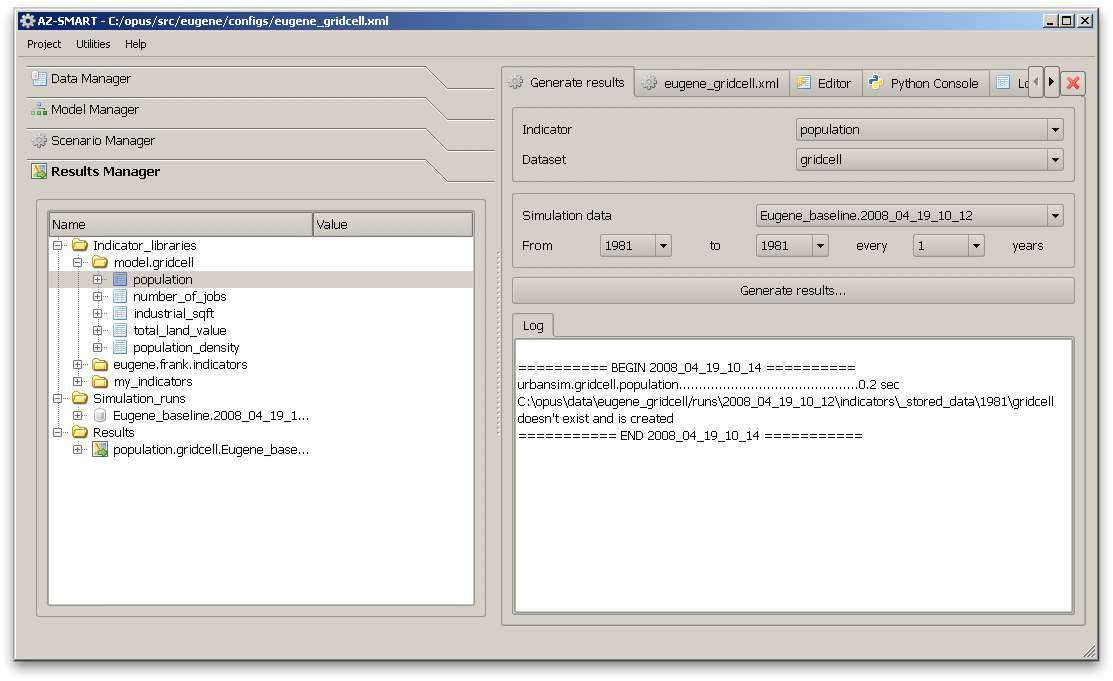
\includegraphics[scale=0.4]{graphics/opus-indicator-2.png}
% \end{center}
% \caption{Result of Generating an Indicator}
% \label{fig:opus-indicator-2}
% \end{figure}
% 
% Now that an indicator has been computed, its data is available to
% visualize or export to another application.  The Results Manager
% currently supports several ways to visualize an indicator, and these
% will depend on the nature of the indicator.  The menu for this is shown
% in Figure \ref{fig:opus-indicator-view-1}.  For example, the indicator
% that has just been computed is population by gridcell.  It is possible
% to visualize data on a grid using a simple image map, displayed on the
% right hand window using the Matplotlib Python library.   If you select
% the Map (Matplotlib) option on the menu, it will generate a map such as
% the one shown in Figure \ref{fig:opus-indicator-view-2}.
% 
% \begin{figure}[htp]
% \begin{center}
% 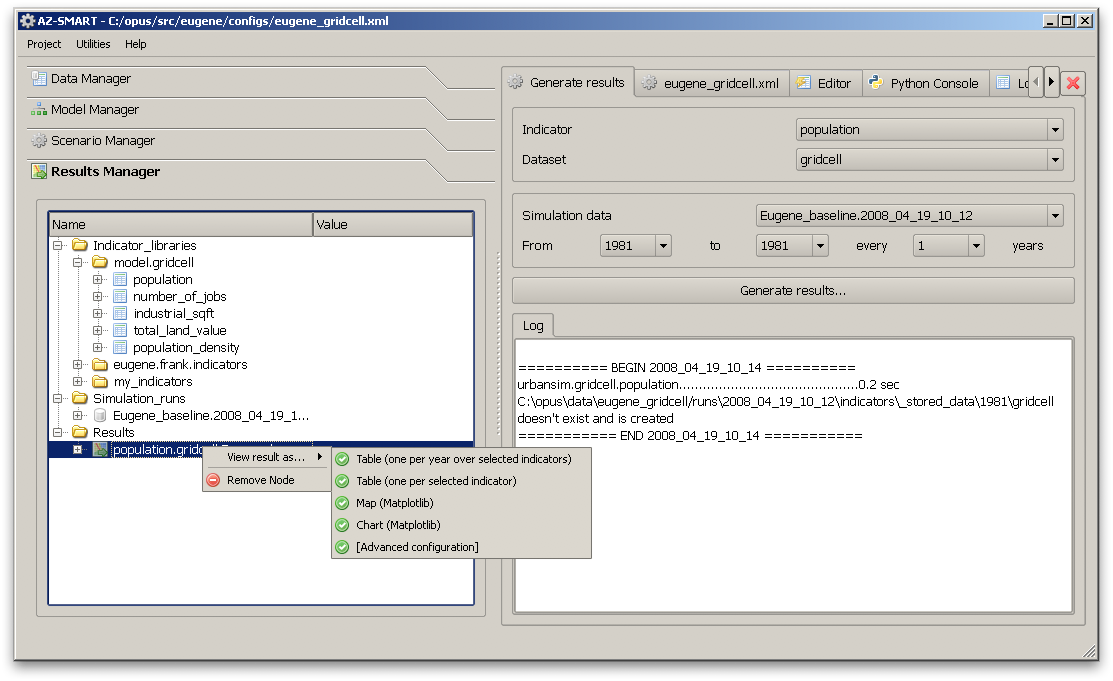
\includegraphics[scale=0.4]{graphics/opus-indicator-view-1.png}
% \end{center}
% \caption{View Results for an Indicator}
% \label{fig:opus-indicator-view-1}
% \end{figure}
% 
% \begin{figure}[htp]
% \begin{center}
% 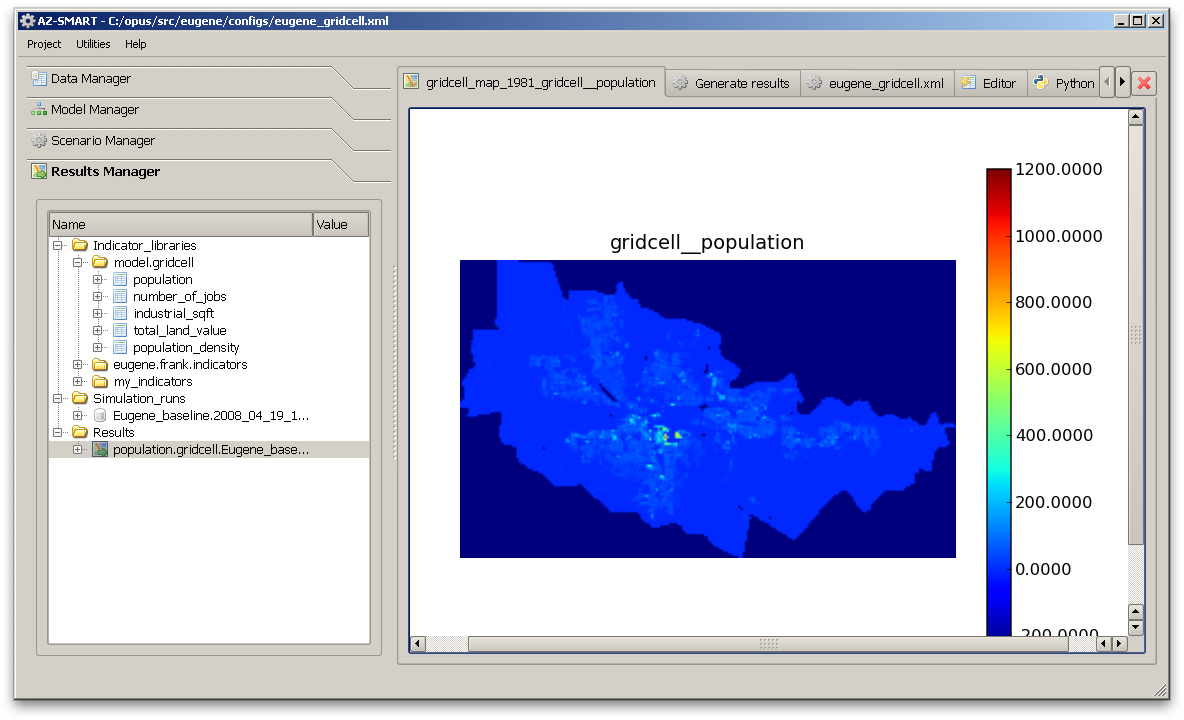
\includegraphics[scale=0.4]{graphics/opus-indicator-view-2.png}
% \end{center}
% \caption{Matplotlib Map for Population by Gridcell in Eugene-Springfield in 1981}
% \label{fig:opus-indicator-view-2}
% \end{figure}
% 
% The Matplotlib map is not intended to replace GIS-based mapping, which
% allows far more control and the overlay of other features for visual
% reference.  It is merely a quick tool to visualize data to get a sense
% of the spatial patterns in it.  In order to support visualization in a
% GIS environment such as ArcGIS or QGIS, the results may be exported to
% a database or geodatabase environment, and the GIS software used to
% create a more interactive and flexible display of the data.
% 

% incorporate the bayesian-melding file into results-manager when it's ready
% \subsection{Create a Map with Uncertainty}

To generate a map with a different confidence interval bounds, check
the ``Visualize Uncertainty'' check box on the Run indicator batch
window (Figures \ref{fig:results-manager-uncertainty1} and
\ref{fig:results-manager-uncertainty2}).

\begin{figure}[htp]
\begin{center}
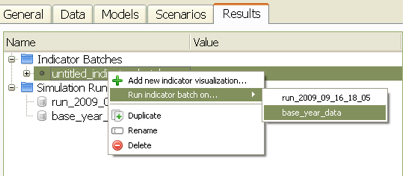
\includegraphics[width=.8\textwidth]{part-gui/images/result-manager-uncertainty1.png}
\end{center}
\caption{The ``Run Indicator Batch'' window}
\label{fig:results-manager-uncertainty1}
\end{figure}


\begin{figure}[htp]
\begin{center}
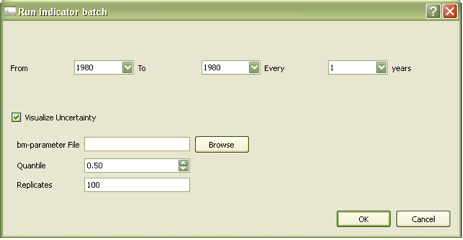
\includegraphics[width=.8\textwidth]{part-gui/images/result-manager-uncertainty2.png}
\end{center}
\caption{Checking the ``Visualize Uncertainty'' box}
\label{fig:results-manager-uncertainty2}
\end{figure}

A {\bf bm-parameter file} is used to specify bias and variance value for a
certain indicator. You must provide a bm-parameter file that has the
following structure:

{\bf first line}: base_year calibration_year \\
{\bf 2 lines per variable}: \\
\hspace*{1cm} 1. variable_name \\
\hspace*{1cm} 2. bias variance

Here is an example:
\begin{verbatim}
1979 1980
urbansim_parcel.zone.number_of_jobs
100 1000
urbansim.gridcell.population_density
7 14
urbansim.gridcell.population
5 14
\end{verbatim}

{\bf Quantile} ranges from 0.01 to 1.00. It has a default value of
0.50, which will generate a map that shows the median. Changing the
quantile value will give you the lower or upper bound for a different
confidence interval. For example, if you wish to see the lower bound
for a Confidence Interval of 90\%, since $(1-0.9)/2 = 0.05$, $0.05$ is
the quantile value that should be entered.  This means that 90\% of
the time, the values indicated on the map will be the lowest possible
values.

{\bf Replicates} has a default value of 100. When a bm-parameter file
is given, an array of size replicate is generated. Replicate value
increases accuracy.


\chapter{XML-based Project Configurations and Inheritance}
\label{chapter:xml-inheritance}

As previously discussed, Opus uses XML-based configuration files to
flexibly specify the various aspects of a project as well as to specify the
appearance of the different tabs in the GUI\@.

One configuration (the \emph{child}) can inherit from another configuration
(the \emph{parent}).  By default, the child inherits all the information
contained in the project.  However, it can override any information
inherited from the parent, and add additional information.  This means that
you can use default projects as parents for another project you want to
create that is mostly the same as an existing project, but has some changes
from it.  An XML configuration specifies its parent using the \emph{parent}
entry under the ``General'' section of the XML\@.  The value of this is the
name of the XML file that contains the parent configuration.  When
searching for this file, Opus first looks in the same directory that holds
the child configuration.  If it's not found there, it expects to find a
path in the Opus source code tree, starting with the name of a project like
\package{eugene} or \package{urbansim}.

This works well with the convention that users should create their own
projects in the \file{opus/project_configs} directory.  You can have
several configurations in your \file{opus/project_configs} directory, one
inheriting from the other.  Ultimately, though, one or more of these
configurations should inherit from a default configuration in the source
tree.  For example, Figure \ref{fig:eugene-gridcell-xml-default} shows the
contents of the default project for \file{eugene_gridcell} in
\file{opus/project_configs}.  This has almost no content of its own, but
rather inherits almost everything from the default configuration in the
source tree at \file{eugene/configs/eugene_gridcell.xml}.

\begin{figure}[htp]
\begin{center}
\begin{verbatim}
<opus_project>
  <general>
    <description type="string">Minimal user configuration for the Eugene 
        gridcell project</description>
    <parent type="file">eugene/configs/eugene_gridcell.xml</parent>
  </general>
</opus_project>
\end{verbatim}
\end{center}
\caption{Contents of the default eugene\_gridcell.xml project}
\label{fig:eugene-gridcell-xml-default}
\end{figure}

A small section of the \file{eugene/configs/eugene_gridcell.xml} file is
shown in Figure \ref{fig:opus-xml}.  It is just text, but in a structured
format, with nodes corresponding to information that is displayed in the
GUI.  Some of the content of the XML provide data used by the GUI to
determine how to display information, or what menu items are appropriate to
connect to the node in the GUI.  Notice that this project in turn inherits
from \file{urbansim_gridcell/configs/urbansim_gridcell.xml}.

\begin{figure}[htp]
\begin{center}
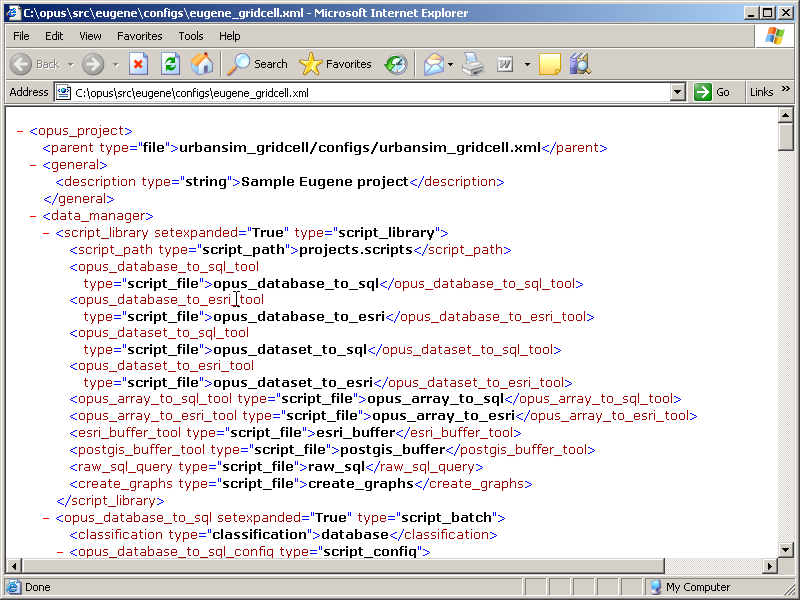
\includegraphics[scale=0.4]{graphics/opus-xml.png}
\end{center}
\caption{An Excerpt from eugene/configs/eugene\_gridcell.xml}
\label{fig:opus-xml}
\end{figure}

To change any of the options in the XML tree you need to be able to edit
it.  Inherited parts of the XML tree are shown in blue in the left pane in
the GUI\@.  These can't be edited directly --- they just show inherited
information.  You can make an inherited portion of the XML tree editable by
right clicking on it and selecting `Add to curent project.''  This copies
the inherited information into the local XML tree.  (We saw an example of
doing this in Section \ref{sec:configuring-scenario}.)

A few details about the ``Add to current project'' command: in Section
\ref{sec:configuring-scenario}, when we added \code{lastyear} to the
current project, the containing nodes in the tree (\code{years_to_run} and
\code{Eugene_baseline}) also turned black, since they needed to be added to
the current project as well to hold \code{lastyear}.  It's also possible to
click directly on \code{years_to_run}, or even \code{Eugene_baseline}, and
add the XML tree under that to the current project.  However, we recommend
adding just the part you're editing to the current project, and not others.
(You can always add other parts later.)  The reason is that once a part of
the tree is added to the current project, the inheritance relation of that
part with the parent disappears, and changes to the parent won't be
reflected in the child XML\@.  For example, if you add all of the
\code{Eugene_baseline} node to the current project, save your
configuration, and then update the source code, changes to some obscure
advanced feature in the XML in the parent in the source tree wouldn't show
up in your configuration.



% Copyright (c) 2005-2009 Center for Urban Simulation and Policy Analysis,
% University of Washington.  Permission is granted to copy, distribute and/or
% modify this document under the terms of the GNU Free Documentation License,
% Version 1.2 or any later version published by the Free Software Foundation;
% with no Invariant Sections, no Front-Cover Texts, and no Back-Cover Texts.
% A copy of the license is included in the section entitled "GNU Free
% Documentation License".

% This is the root latex source file for the Opus and UrbanSim Users Guide.
% The guide is organized as a set of 'include' files, normally one file
% per chapter.  It uses the Python latex documentation standards and latex
% definition files -- see http://www.python.org/doc/current/doc/doc.html
% Also see the "Writing Documentation" chapter in this manual for more
% information.


\part{OPUS Data and Models}\label{part-user-guide}

\chapter{Data in Opus}
\label{chap:data-in-opus}

\emph{This chapter is under construction...}

Datasets are analogous to tables in a database. Attributes
are analogous to columns in a database table. e.g. geographical
datasets, households...

\section{Primary and Computed Attributes}

\section{Importing and Exporting Data}

\chapter{Creating Variables in Opus}


Opus is implemented in the Python programming language, so we begin
with a review of the language in Section \ref{sec:python}. Numpy is a numerical library for Python that is used exensively in the
Opus system, so this is covered in Section \ref{sec:numpy}. Using
Python and Numpy, many of the Opus Variables are coded as modules, and
these are explained in Section \ref{sec:variables}.  Finally, a recent
and extremely valuable addition to the Opus architecture is a small
language for Opus Expressions, which makes the need to code variables
as separate modules unnecessary in most cases.  The expression language
is the subject of Section \ref{sec:expressions}.



\section{Opus Expressions}
\label{sec:expressions}
\index{expressions}

Opus uses Python and Numpy to create variables to be used in models.  These are generally coded in Python modules as
described in the preceding section.  However, in order to make the use of variables simpler for users to access, a new
\emph{expression language} has been created for Opus
that allows variables to be defined with a relatively simple and concise syntax.  

The syntax consists of using Numpy operations and methods, operating on Opus variables and primary data.  All of the Numpy operators are available, and work in the same way for expressions, including \verb#+ -  * / **#, where ** is an exponential function: a**3 returns a to the power of 3.

Expressions allow an \verb#alias#, or name, to be assigned to the expression, in order to use it by this reference in a model specification or indicator function.  The standard syntax in Opus uses short names, with lower case letters.  If two or more words are used in a name, we usually separate the components with an underscore to make the name more readable.  Some examples will illustrate key aspects of the expression syntax:

\begin{itemize}

\item \code{hwy\_300 = gridcell.distance\_to\_highway<300} would generate a dummy variable equal to 1 for gridcells that have an attribute value of distance to highway less than 300 meters.  Note that in this case we are operating on a \verb#primary attribute# of gridcells, which means that it is part of the data that we initially load into the model, as opposed to data we compute within the model.

\item \code{ln\_pop = ln(urbansim.gridcell.population} would be used to compute the log of an existing variable, population, which is in the urbansim package and applies to the gridcell dataset.

\item \code{pop\_emp\_ratio = urbansim.gridcell.population / urbansim.gridcell.number\_of\_jobs} would compute the ratio of population to employment, using variables stored in the urbansim package, associated with the gridcell dataset.  

\end{itemize}

Two very useful methods in the expression language are \verb#aggregation# and \verb#disaggregation#.  Aggregation allows an expression to compute a result on one dataset and aggregate the results to assign to another dataset, such as summing the population in households that live in a gridcell.  Using this expression approach, we could replace the long population.py module in the preceding section with the following expression:

\code{population = gridcell.aggregate(household.persons)}

That is quite a lot easier to understand and to code!  We are aggregating to the gridcell dataset, from the household dataset, the number of persons.  However, in the time since the variable in the preceding section was implemented, we have changed the data structure for the gridcell and parcel based models to use buildings.  So now, households and jobs are associated with buildings, and buildings are associated with gridcells (or parcels).  This means that in order to compute the population of a gridcell, we need to first aggregate it to building, and then from building to gridcell.  That is not hard to do, either, by simply adding an intermediated argument to the aggregation function.  There can be multiple levels of intermediates, if needed:

\code{population = gridcell.aggregate(household.persons, intermediates = [building])}

The default method for aggregation is to sum, but there are several other aggregation methods available also:

\squishlist
\item sum
\item mean
\item maximum
\item mininim
\item variance
\item standard\_deviation
\item center\_of\_mass
\squishend

To use any of these functions, we simply add \verb#function = mean# (or another function) in the expression.  Here is an example to determine the average household size per gridcell:

\code{avg\_hhs = gridcell.aggregate(households.persons, intermediates = [building], function = mean)}

The \verb#disaggregate# method for expressions assigns values from one dataset to another, in a one to many relationship.  In other words, it works in the opposite direction from the aggregate method, which is many to one.  An example would be to assign the zonal population density to all households living the zone.  In this example, we use the \verb#population_density# variable in the zone dataset of the urbansim\_parcel package, and assign it to households, which are connected to zones indirectly through buildings and then parcels: household -$>$ building -$>$ parcel -$>$ zone.  So the expression would be:

\code{density = household.disaggregate(urbansim\_parcel.zone.population\_density, intermediates = [building, parcel])}

Note that for both aggregate and disaggregate methods, the first element, preceding the method name, is the name of the dataset to which the result should be assigned.  zone.aggregate... should generate some result and assign it to zone, whereas gridcell.disaggregate... should assign some value from a larger geography to the gridcell dataset.

A list of expressions can be stores in an \verb#aliases.py# file within a package and dataset directory.  This provides an efficient means to organize and store many expressions in a single location.  Below are some of the aliases in the urbansim\_parcel/parcel/aliases.py module that demonstrate some of the expressions in actual use in the model system.\\

\begin{lstlisting}
"used_land_area = (parcel.aggregate(building.land_area, function=sum)).astype(int32)",
"vacant_land_area = parcel.parcel_sqft - urbansim_parcel.parcel.used_land_area",
"unit_name = parcel.disaggregate(land_use_type.unit_name)",
"building_sqft = (parcel.aggregate(urbansim_parcel.building.building_sqft)).astype(int32)",
"building_sqft_per_unit = safe_array_divide(urbansim_parcel.parcel.building_sqft, urbansim_parcel.parcel.residential_units)",
"residential_units = (parcel.aggregate(building.residential_units)).astype(int32)",       
"parcel_sqft_per_unit = safe_array_divide( parcel.parcel_sqft, (urbansim_parcel.parcel.residential_units).astype(float32) )",
"unit_price = safe_array_divide(parcel.land_value + urbansim_parcel.parcel.improvement_value, urbansim_parcel.parcel.existing_units)",
"demolition_cost = (parcel.aggregate(urbansim_parcel.building.demolition_cost)).astype(int32)",
"improvement_value = (parcel.aggregate(building.improvement_value)).astype(int32)",
"total_value_per_sqft = safe_array_divide(parcel.land_value + urbansim_parcel.parcel.improvement_value, parcel.parcel_sqft)",
"number_of_jobs = parcel.aggregate(urbansim_parcel.building.number_of_jobs)",
"employment = parcel.aggregate(urbansim_parcel.building.number_of_jobs)",
"number_of_households = parcel.aggregate(urbansim_parcel.building.number_of_households)",
"population = parcel.aggregate(urbansim_parcel.building.population)",
"travel_time_to_cbd = parcel.disaggregate(gridcell.travel_time_to_cbd)",       
\end{lstlisting}

\section{Opus Indicators}

Indicators are typically considered summary measures used for evaluation purposes, like a cost-benefit ratio, or a VMT per capita measure.  Indicators can also be used for evaluation purposes.  Opus has a fairly extensive infrastructure for computing indicators.  Some of it is already available in the new Opus GUI, but there is more functionality available using scripts.  In the eugene package, for example, there is an indicators directory containing a make\_indicators.py script that demonstrates the use of a script to make a series of different kinds of indicators.  A more extensive set of examples and documentation is provided in the script  /opus/src/opus\_core/indicator\_framework/make\_indicators\_example.py.

Indicators generally use expressions to do their computation, so they share all of the functionality described in the preceding section.  The Opus Indicator Framework, however, adds some very helpful methods to also visualize the results of the indicator computation, or to export the results to a text file, or a table in a database, or to a GIS for visualization.

The indicator output options currently include the following types:

\squishlist
\item \emph{Map}: produces a map of the indicator rendered in Matplotlib. This works only on a gridcell-based indicator, but can include more aggregate indicators if they can be assigned to gridcells using a disaggregate function, such as \code{gridcell.disaggregate(zone.population\_per\_acre)}.
\item \emph{Chart}: produces a simple line chart, useful for tracking an aggregate indicator over multiple years of a simulation.
\item \emph{Table}: produces a browsable table that can also be exported, containing two columns: the column containing the level of geography or aggregation, and the column containing the indicator value for that aggregation.  A zone table of total population would be an example of this form.
\item \emph{DatasetTable}: produces a table with multiple indicators for the same unit of aggregation or geography, such as employment by zone, with multiple columns representing the total employment for each industry sector, and possibly other indicators.  It would contain one record per zone.
\squishend

The Opus GUI currently supports the first three of these types directly, and provides a means to generate the DatasetTable type of indicator output, though the interface for this is being revised significantly.  The following tutorial focuses on the use of the GUI to create and visualize several different kinds of indicators.  

Assume that we want to run the eugene\_gridcell baseline scenario from 1980 to 1990, and then will generate the following indicators from the simulation results:

\squishlist
\item Average cars per household by gridcell, viewed as a map
\item Average cars per household by zone, viewed as a map
\item Log of the sum of population and employment by gridcell, as a map
\item Average household size per zone, viewed as a table
\item Total population by year, as a chart
\item Total population by zone, as a table
\squishend

For the first indicator, we need an expression that would compute the average number of cars for the households living in a gridcell, and then to display this on a map.  The expression is straightforward:

\code{cars\_per\_hh = gridcell.aggregate(household.cars, function=mean)}

Note that since we are operating on a \verb#primary attribute# of the data (we can find \verb#cars# in the data directory under data/eugene\_gridcell/household), we do not need to put a package name in the expression.  We could leave out the alias \verb#cars_per_hh =#, but when we generate the indicator and map, using an alias will provide a meaningful default title on the Matplotlib map.

To create and visualiza this indicator in the Opus GUI, open the eugene\_gridcell project.  If you have not previously run a simulation on the computer you are using, you will need to generate a simulation run first\footnote{In the Scenario Manager, expand the years\_to\_run node, change the end\_year to something like 1990 to get a longer run, and then start the run}.   Figures \ref{fig:indicator-cars-gridcell-1}-\ref{fig:indicator-cars-gridcell-2} show the user interface steps to create this new indicator, which we will call cars\_hh.  You will need to right-click on \verb#my_indicators# and select \verb#Add to current project# first.  This will make a copy of the indicator configurations locally that is editable.  Once this has been made editable, the color changes from grey to black.  Now right click again and select \verb# New Indicator#, then edit the expression to use the one shown above.  Change the name of the indicator to match also. Since this indicator uses primary attributes only, there is no requirement to specify a package, and this can be left with the default value in the package entry above the expression (a question mark).  You can then generate results with this indicator by selecting a year and a simulation result, and then select the indicator result and generate a Matplotlib map, as shown below.

\begin{figure}[htp]
\begin{center}
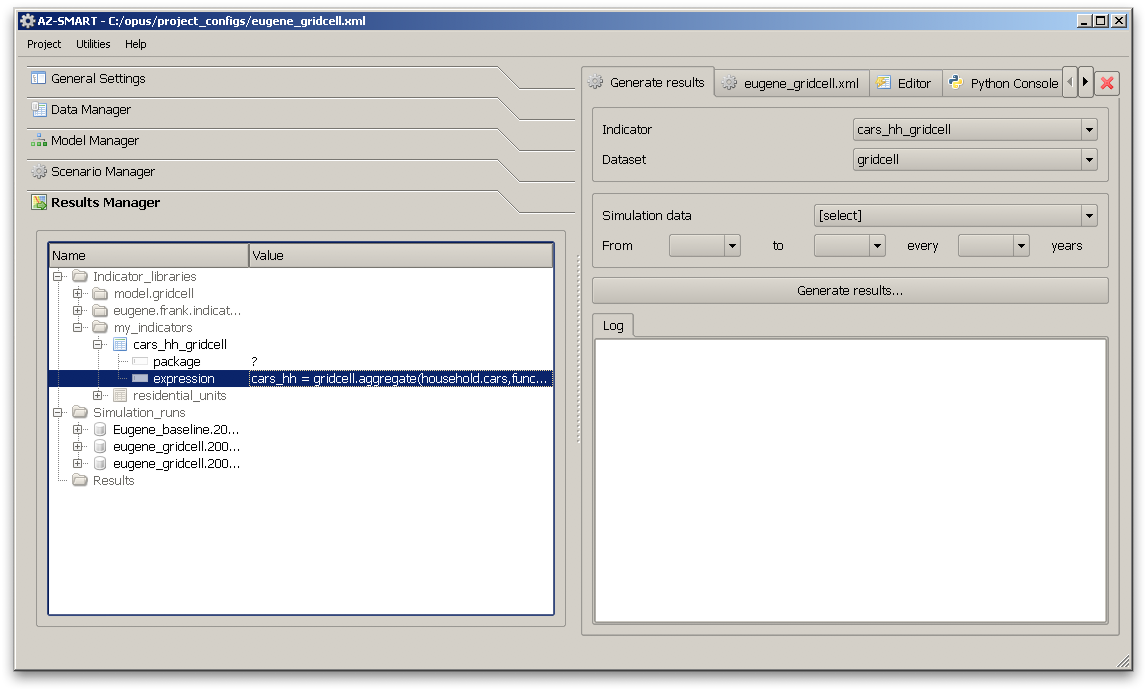
\includegraphics[scale=0.4]{graphics/indicator-cars-gridcell-1.png}
\end{center}
\caption{Generating the Average Cars per Household in a Gridcell}
\label{fig:indicator-cars-gridcell-1}
\end{figure}

\begin{figure}[htp]
\begin{center}
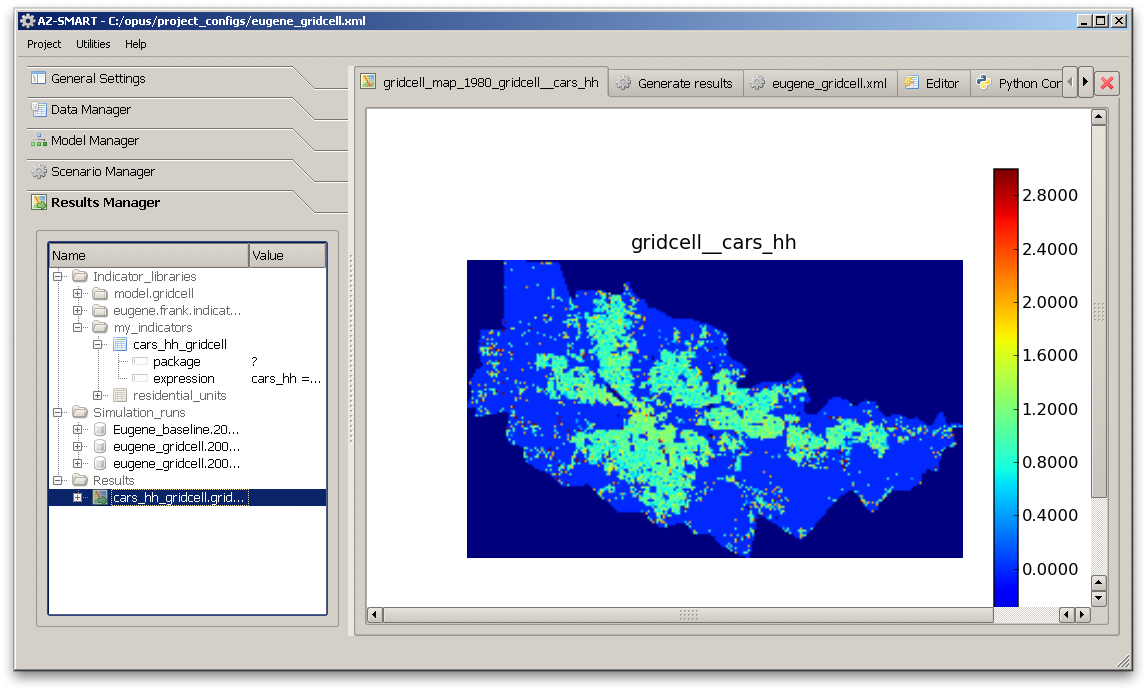
\includegraphics[scale=0.4]{graphics/indicator-cars-gridcell-2.png}
\end{center}
\caption{Generating the Average Cars per Household in a Gridcell}
\label{fig:indicator-cars-gridcell-2}
\end{figure}

In order to compute the second indicator, we will need to average the number of cars per household at the zonal level as follows:

\code{cars\_per\_hh = zone.aggregate(household.cars, intermediates= [gridcell], function=mean)}

The only remaining problem with this is that we cannot display zonal data using Matplotlib, which generates only raster image maps, meaning that it only supports displaying data assigned to gridcells.  Recalling the \verb#disaggregate# function in the expression language, we can just disaggregate the zonal average like this:

\code{cars\_per\_hh = gridcell.disaggregate(zone.aggregate(household.cars, intermediates= [gridcell], function=mean))}

To generate the third indicator of average household size we could use a similar expression:

\code{persons\_per\_hh = zone.aggregate(household.persons, function=mean, intermediates = [gridcell])}

\emph{Unfortunately this zone aggregation will not currently work in the GUI due to some hard coding that assumes indicators added in my\_indicators will be gridcell-based.  This will be fixed shortly.  In the mean time, it would be better to stick to gridcell-based indicators in the my\_indicators section of the Results Manager.}

Now we use a compound expression, to sum the result of two variables, and take the log of the result.  This is to produce the indicator as shown below:

\code{ln\_emp\_pop=ln(urbansim.gridcell.population+urbansim.gridcell.number\_of\_jobs)}

Note that these are variables which can be found on the disk in src/urbansim/gridcell.  The result of visualizing this indicator is shown in Figure \ref{fig:indicator-ln-emp-pop}.

\begin{figure}[htp]
\begin{center}
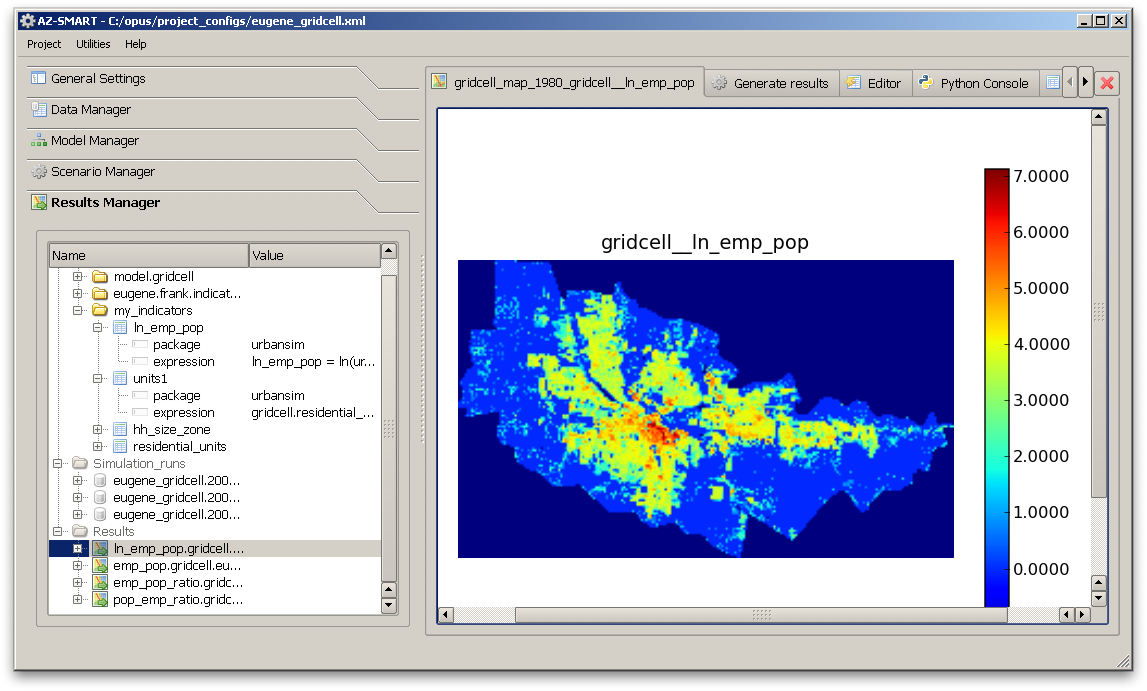
\includegraphics[scale=0.4]{graphics/indicator-ln-emp-pop.png}
\end{center}
\caption{Log of (Population + Employment) by Gridcell}
\label{fig:indicator-ln-emp-pop}
\end{figure}

For the last two indicators in the list to be done, we return to indicators that are already defined in a generic indicator library in the results manager.  To produce the population by zone indicator and visualize it as a table, use the following steps.  Right-click on the population indicators, and select \verb#Generate results with#.  In the form that is created on the right, select the pull-down menu labeled \verb#Dataset# and click on zone.  This is a generalized indicator that uses a simple mechanism to allow different levels of aggregation to be selected in this way, without the need to type in an expression as was done in the preceding examples.  Select a simulation result, and generate the indicator.  Then select the new indicator result containing the indicator values, right-click, and select \verb#View result as# and choose \verb#Table#.  This should generate a browsable table in the form window, as shown below in Figure \ref{fig:indicator-population-zone-table}.

\begin{figure}[htp]
\begin{center}
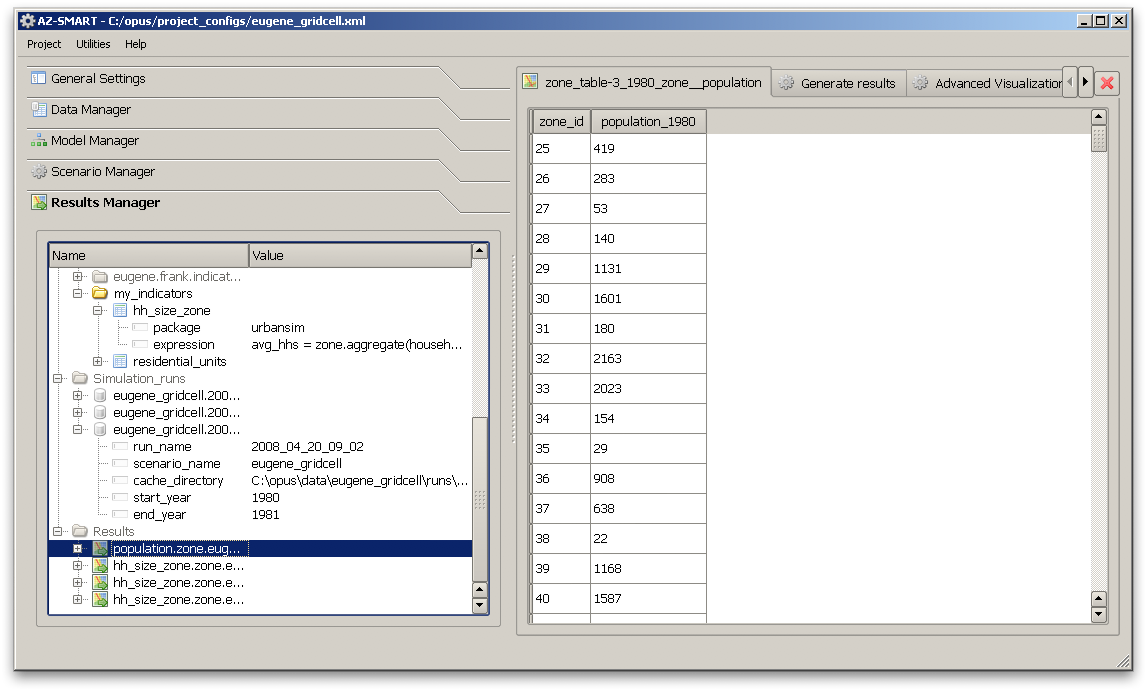
\includegraphics[scale=0.4]{graphics/indicator-population-zone-table.png}
\end{center}
\caption{Viewing the Population by Zone Indicator as a Table}
\label{fig:indicator-population-zone-table}
\end{figure}

Now that we have seen the integrated Matplotlib maps, you might want to know how to export an indicator to a more full-featured GIS system such as ArcGIS (a commercial package from Environmental Systems Research Institute), or PostGIS (an open source package built on the Postgres database).  The Results Manager is now able to export a table with one or more indicators to an ESRI Geodatabase for further analysis and visualization.  In the following example, we export the same indicator result shown above as a table, to an ESRI File-based Geodatabase.  Other Geodatabase formats are also supported.

If the population by zone table result is still available, right-click on the result in the tree on the left-hand side of the window, and select the \verb#View result as# and choose \verb#Advanced visualization#.  It will generate a form as shown in Figure \ref{fig:indicator-population-zone-export}.  We need to add the indicator we have generated to the set, in the upper portion of this form, and select the location of the ESRI geodatabase.  I am assuming that the geodatabase contains a \verb#Feature Class# corresponding to the table being exported. In this example, the table corresponds to the zone feature class.  Once the form is filled in, click on the \verb#Go!# button, to start the export process.  A message will be printed to the log to indicate the completion status of this export process.

\begin{figure}[htp]
\begin{center}
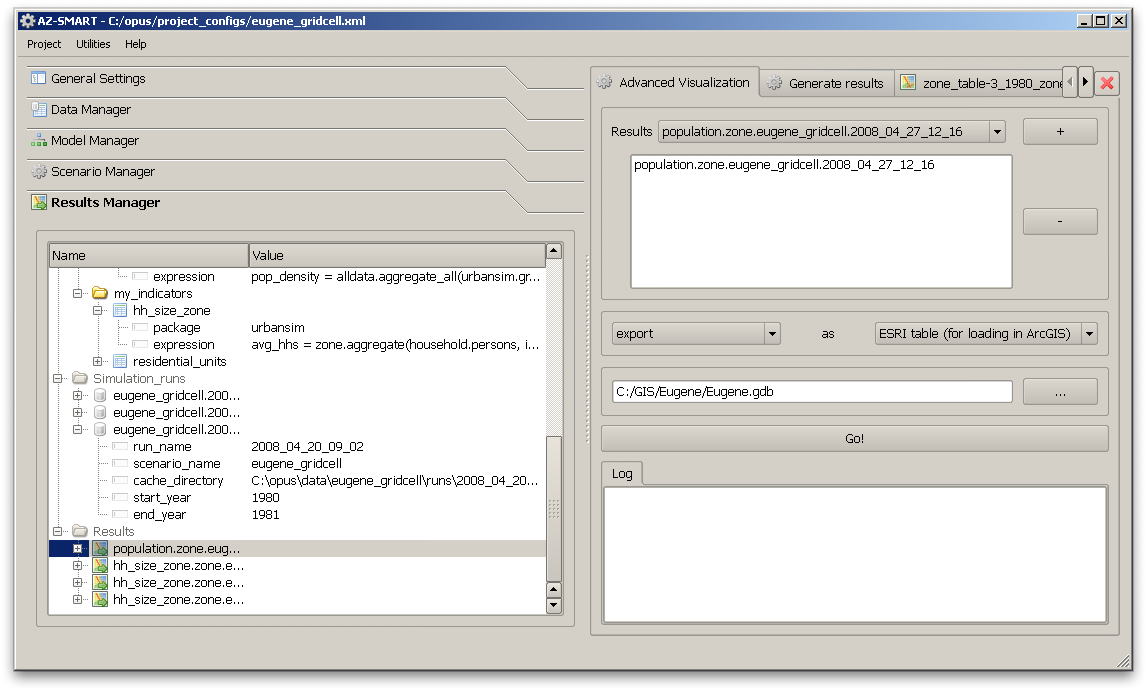
\includegraphics[scale=0.4]{graphics/indicator-population-zone-export.png}
\end{center}
\caption{Exporting the Population by Zone Indicator to an ESRI Geodatabase}
\label{fig:indicator-population-zone-export}
\end{figure}

Once the export is successfully completed, the geodatabase will contain a table that contains the indicator result, with a zone\_id and an ArcGIS \verb#OBJECTID*# that corresponds to the internal object ids in the feature class.  It is safe to join the indicator table result with the feature class using either the objectid or the zone\_id.  The map in Figure \ref{fig:indicator-population-zone-arcgis} shows the result of joining the feature class with the indicator table and generating a thematic map of the populaion by zone, using the zone.acres field to normalize the population, resulting in a map of population density per acre.

\begin{figure}[htp]
\begin{center}
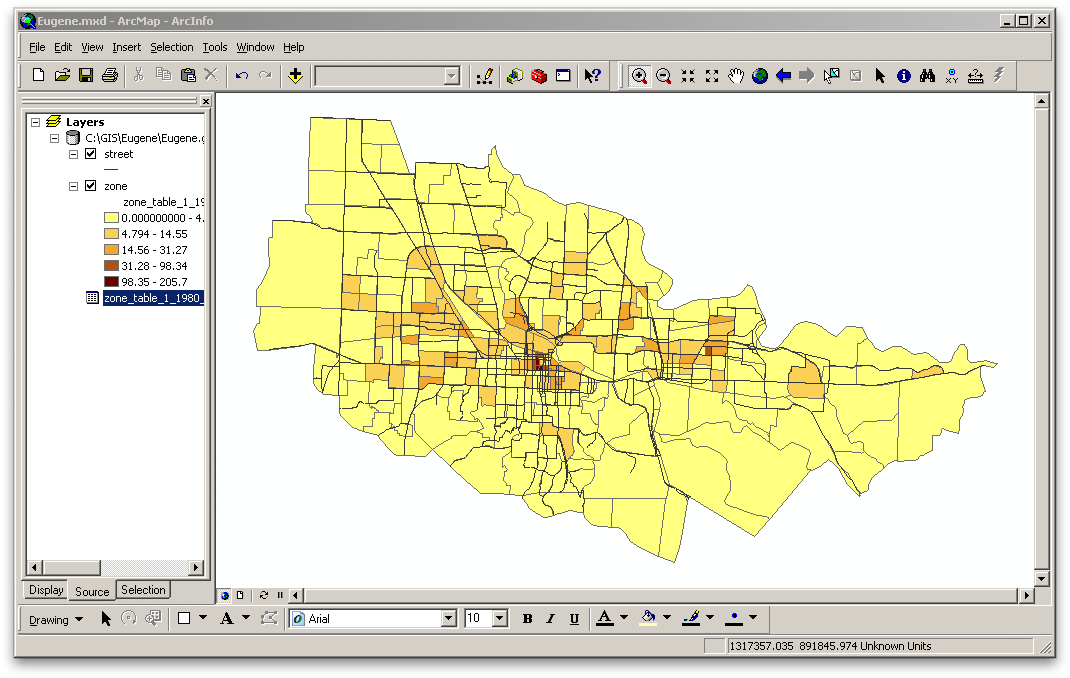
\includegraphics[scale=0.4]{graphics/indicator-population-zone-arcgis.png}
\end{center}
\caption{Mapping the Population by Zone Indicator in ESRI ArcMap}
\label{fig:indicator-population-zone-arcgis}
\end{figure}

\section{(advanced) Creating New Opus Variables}
\label{sec:variables}

Variables in Opus are Python modules containing a single Python \verb#Class# that computes a variable and returns the result.  For demonstration purposes, the population variable in \verb#/src/urbansim/gridcell/population.py# is shown below.  We refer to a variable using a \verb#Pythonpath#, which provides a means for Python to find modules and classes in a directory structure.  So, a reference to this particular module using a \verb#fully qualified path# would be \verb#urbansim.gridcell.population#.  You can find all of the existing variables by browsing on disk in the source code directory.  The directory structure mirrors the parts of the variable name, so that urbansim.gridcell.population is really pointing to /opus/src/urbansim/gridcell/population.py, which is included below as an example.

\begin{lstlisting}
from opus_core.variables.variable import Variable
from urbansim.functions import attribute_label
from variable_functions import my_attribute_label
from opus_core.logger import logger

class population(Variable):
    """Compute the total number of people residing in a gridcell, 
    by summing hh_persons over all households in the gridcell"""
    
    _return_type="int32"
    hh_persons = "persons"

    def dependencies(self):
        return [attribute_label("household", self.hh_persons), 
                attribute_label("household", "grid_id"), 
                my_attribute_label("grid_id")]

    def compute(self, dataset_pool):
        households = dataset_pool.get_dataset('household')
        return self.get_dataset().sum_dataset_over_ids(households, self.hh_persons)


from opus_core.tests import opus_unittest
from opus_core.tests.utils.variable_tester import VariableTester
from numpy import array
class Tests(opus_unittest.OpusTestCase):
    def test_my_inputs(self):
        gridcell_grid_id = array([1, 2, 3])
        #specify an array of 4 hh's, 1st hh's grid_id = 2 (it's in gridcell 2), etc.
        household_grid_id = array([2, 1, 3, 2]) 
        #specify how many people live in each household
        hh_persons = array([10, 5, 20, 30])

        tester = VariableTester(
            __file__,
            package_order=['urbansim'],
            test_data={
                "gridcell":{
                    "grid_id":gridcell_grid_id 
                    }, 
                "household":{ 
                    "household_id":array([1,2,3,4]),
                    "persons":hh_persons, 
                    "grid_id":household_grid_id
                }
            }
        )
        
        should_be = array([5, 40, 20])
        tester.test_is_close_for_family_variable(self, should_be)

if __name__=='__main__':
    opus_unittest.main()
\end{lstlisting}

Some new features presented in this example are the use of a Python Class, which is a topic I will defer for now, the use of dependencies (other variables or primary attributes of datasets that the current variable depends on), and the use of tests in code to ensure that the computation is doing what is expected.  The use of Python modules containing a Class to compute a single variable is flexible and quite powerful, but a bit too complex for most users to use on a regular basis, especially if what is desired is a simple transformation of an attribute or a variable.  Until recently, even something as simple as taking the logarithm of this population variable would have required writing a new module to to that transformation.  Fortunately, this is no longer necessary, since a new Opus Expression language has been implemented.

\chapter{Creating Models in Opus}
\label{chap:creating-models}
\section{Model Types in Opus}

Opus provides infrastructure to develop, specify, estimate,
diagnose and predict with a variety of model types.  The
Opus GUI currently supports the creation of several types of
models by providing templates that can be copied and
configured. More will be added in the future.  These initial
types are:

\squishlist
\item Simple Models
\item Sampling Models
\item Allocation Models
\item Regression Models
\item Choice Models
\item Location Choice Models
\squishend 

\subsection{Simple Models}
%
\label{sec:components-simple-model}
\index{models!opus_core models!simple model}
%
The simplest form of a model in Opus is called, for lack of
imagination, Simple Model.  It is about as simple as a model
can get: compute a variable and write the results to a
dataset.  Here are some examples of what could be done with
a simple model:

\squishlist
\item Aging Model: add one to the age of each person, each
  year
\item Walkability Model: write the result of an expression
  that evaluates the amount of retail activity within
  walking distance
\item Redevelopment Potential Model: compute the ratio of
  improvement to total value for each parcel and write this
  to the parcel dataset \squishend

  A Simple Model template is available in the Model Manager,
  and can be copied and configured in order to create a new
  Simple Model like the examples above. It takes only three
  arguments in its configuration:

\squishlist
\item Dataset: the Opus Dataset that the result will be
  written to
\item Outcome Attribute: the name of the attribute on the
  Dataset that will contain the predicted values
\item Expression: the Opus Expression that computes the
  result to be assigned to the outcome attribute \squishend

\subsection{Sampling Models}
The second type of model template is a Sampling Model.  This
generic model takes a probability (a rate), compares it to a
random number, and if the random number is larger than the
given probability (rate), it assigns the outcome as being
chosen.  Some examples will make the use of this model
clearer. Say we want to build a household evolution model.
We need to deal with aging, which we can do with a Simple
Model.  We also models that predict:

\squishlist
\item Births
\item Deaths
\item Children leaving home as they age
\item Divorces
\item Entering the labor market
\item Retiring
\squishend

For all of these examples -- assuming that we want to base
our predictions on expected rates that vary by person or
household attributes -- we need a more sophisticated model
that we shall call a Sampling Model.  Since we need to
assign a tangible outcome rather than a probability, we use
a sampling method to assign the outcome in proportion to the
probability.  This method is also occasionally referred to
as a Monte Carlo Sampling algorithm.

The algorithm is simple.  Let's say we have a probability of
a coin toss, heads or tails each having a probability of
0.5.  A sampling model to predict an outcome attribute of
Heads, would take the expected probability of a fair coint
toss resulting in an outcome of Heads as being 0.5.  We then
draw a random number from a univariate distribution between
0 and 1, and compare it to the expected probability. If the
random draw is greater than the expected probability, then
we set the choice outcome to Heads.  If it is less than 0.5,
then we set the choice outcome to Tails.  Since we are
drawing from a univariate random distribution between 0 and
1, we would expect that around half of the draws would be
less than 0.5 and half would be greater than this value.
Larger numbers of draws will tend to converge towards the
expected probability by the law of large numbers.  A very
large number of draws should match the expected probability
to a very high degree of precision.

To make the model useful for practical applications, we can
add a means to apply different probabilities to different
subsets of the data.  For example, death rates or birth
rates vary by gender, age, and race/ethnicity, and to some
extent by income.  We might want to stratify our
probabilities by one or more of these attributes, and then
use the sampling model to sample outcomes using the expected
probabilities for each subgroup.

The Sampling Model takes the following arguments:

\squishlist
\item Outcome Dataset: the name of the dataset to receive the predicted values
\item Outcome Attribute: the name of the attribute to contain the predicted outcomes
\item Probability Dataset: the name of the dataset containing the probabilities
\item Probability Attribute: the name of the attribute
  containing the probability values (or rates)
\item List of Classification Attributes: attributes of
  Outcome Dataset that will be used to index different
  Probabilities (e.g. age and income in household
  relocation) \squishend

\subsection{Allocation Models}
%
\label{sec:components-allocation-model}
\index{models!opus_core models!allocation model}
%
Another simple generic model supported in Opus is the
Allocation Model, which does not require estimating model
parameters.  This model proportionately allocates some
aggregate quantity to a smaller unit of analysis using a
weight.  This model could be configured, for example, to
allocate visitor population estimates, military population,
nursing home population, and other quantities to traffic
analysis zones for use in the travel model system.  Or it
could be used to build up a simplistic incremental land use
allocation model (though this would not contain much
behavioral content).

The algorithm for this type of model is quite simple.  To
create an Allocation Model, we need to specify six
arguments:

\squishlist
\item Dataset to contain the new computed variable
\item Name of the new computed variable $Y$, which will be
  indexed by the ids of the dataset it is being allocated
  to, $Y_i$.
\item Dataset containing the total quantity to be allocated
  (this can contain a geographic identifier, and will
  include a year column).
\item Variable containing the control total to be allocated,
  $T$
\item Variable containing the (optional) capacity value $C$,
  indexed as $C_i$
\item Variable containing the weight to use in the
  allocation $w$, indexed as $w_i$, with a sum across all
  $i$ as $W$ \squishend

The algorithm is then just:

\begin{equation}
Y_i = min(round(T\frac{w_i}{W}),C_i)
\end{equation}

If a capacity variable is specified, we add an iterative
loop, from $m$ to $M$, to allocate any excess above the
capacity to other destinations that still have remaining
capacity:

\begin{equation}
T^m = sum(round(T\frac{w_i}{W}) - C_i)
\end{equation}

In each iteration, we exclude alternatives where $Y>=C$, and
repeat the allocation with the remaining unallocated total:

\begin{equation}
Y^m_i = Y^{m-1}_i + (T_m\frac{w_i}{W})
\end{equation}

We then iterate over $m$ until $T^m = 0$ 

This simple algorithm is fairly versatile, and can be used
in two modes: as incremental growth or as total values. If
used in incremental mode, it adds the allocated quantity to
the existing quantities.  The alternative, total, mode for
this model replaces the quantities with the new predicted
values.

\subsection{Regression Models}
%
\label{sec:components-regression-model}
\index{models!opus_core models!regression model}


Regression models are available to address problems in which
the dependent variable is continuous, and a linear equation
can be specified to predict it.  The primary use of this
model in a core model in UrbanSim is the prediction of
property values.  In the context of predicting property
values, the model is referred to as a hedonic regression
\cite{waddell-hedonic-1993}, but the Opus regression model
is general enough to address any standard multiple
regression specification.  Other examples of applications
for this basic class of models would be to predict water or
energy consumption per household, or parking prices.

The basic form is:

\begin{equation}
Y_i = \alpha + \beta X_i + \epsilon_i
\end{equation}

where $X_i$ is a matrix of explanatory, or independent,
variables, and $\beta$ is a vector of estimated parameters.
Opus provides an estimation method using Ordinary Least
Squares, and additional estimation methods are available by
interfacing Opus with the R statistical package.  For the
current discussion, we focus on working with the built-in
estimation capacity.

\subsection{Choice Models}
%
\label{sec:components-choice-model}
\index{models!opus_core models!choice model}
%

Many modeling problems do not have a continuous outcome, or
dependent variable.  It is common to have modeling problems
in which the outcome is the selection of one of a set of
possible discrete outcomes, like which mode to take to work,
or whether to buy or rent a property.  This class of problem
we will refer to as discrete choice situations, and we
develop choice models to address them.

Recall from Section \ref{sec:discrete-choice} that the
standard multinomial logit model
\cite{mcfadden-1974,mcfadden-1981} can be specified as:

\begin{equation}
    P_i = \frac{\mathrm{e}^{V_i}}{\sum_j \mathrm{e}^{V_j}},
\end{equation}
where $j$ is an index over all possible alternatives,
$V_i = \beta\cdot {x}_i$ is a linear-in-parameters
function, $x_i$ is a vector of observed, exogenous, independent
alternative-specific variables that may be interacted with the
characteristics of the agent making the choice,
and $\beta$ is a vector of $k$ coefficients
estimated with the method of maximum likelihood \cite{greene-2002}.

The multinomial logit model is a very robust and widely used
model in practical applications in transportation planning,
marketing, and many other fields.  It is easy to compute and
is therefore fast enough to use on large-scale computational
problems such as residential location choice.  For
explanatory purposes, we will focus initially on choice
problems with small numbers of alternatives, such as the
choice to rent or own a house, or the number of vehicles a
household will choose to own.

Note that there are limitations to the MNL model, and
assumptions a user should be aware of.  The most important
of these is the Independence of Irrelevant Alternatives
(IIA) property, which implies that adding or eliminating an
alternative from a choice set will affect all of the
remaining alternatives proportionately.  Stated another way,
the relative probabilities of any two alternatives will be
unaffected by adding or removing another alternative.  See
\cite{train-book-2003} for a thorough introduction to
discrete choice modeling using MNL and other choice model
specifications.

We now turn to a tutorial for creating models of some of
these types using the Opus GUI.  In the following sections,
we provide a worked example of creating a new model of each
type.  The other model types follow the same pattern in the
Opus GUI.


\section{Interactive Estimation and Diagnostics}
\label{sec:components-model-estimation}
{\bf Please note:} the seattle\_parcel sample data used in the following
description is only to demonstrate functionality.  One should not read too
much into the results, since seattle\_parcel is a small subset taken from
the PSRC project datasets to make its size more manageable.  In particular,
estimating models with certain specifications may give peculiar results,
such as SE and t-values equal to \verb|-1.#IND| or \verb|-1.#INF| due to
an insufficient number of observations, collinearity, or outliers in the
data.  Estimation results that include erroneous results such as these
cannot saved or exported to a sql database, or viewed in the OPUS GUI\@.

\subsection{Estimation of a Regression Model}

In this section, we take up the topic of estimating and diagnosing models
interactively, from the command line.  Eventually the functions described
here will be available in the Graphical User Interface, but as of now they
are only available from the interactive command mode.

Assume we want to estimate the real estate price model in the
seattle\_parcel project, which includes submodels to separately specify the
model for each general land use type.  If you are using a computer with the
Windows operating system, open a command shell, and type the following:

\begin{verbatim}
python -i c:\opus\src\urbansim\tools\start_estimation.py 
-x c:\opus\project_configs\seattle_parcel_default.xml -m real_estate_price_model
\end{verbatim}
(Put this command in one single line or with proper continuation
mark for respective operation system.)

Note that this assumes that your Opus packages are installed in the directory \verb|c:\opus|. 
Also note that the argument of the \verb|-x| option must be given as an absolute path.  

Depending on exactly what the specification is, the result of the call 
would look something like the listing below:
\\

\begin{verbatim}
(clipped results)
...
    ===============================================

    Estimate regression for submodel 28
    Number of observations: 1155
    R-Squared:             0.00277863388614
    Adjusted R-Squared:    0.0010473467922
    Suggested |t-value| >  2.6555330205
    -----------------------------------------------
    Coeff_names	estimate	SE	t-values
       constant	 3.44533	0.307501	 11.2043
       lnempden	0.0281543	0.0176717	 1.59318
      lngcdacbd	 0.15989	0.0943748	 1.69421
    ===============================================

    Estimate regression for submodel 30
    Number of observations: 456
    R-Squared:             0.0678509575502
    Adjusted R-Squared:    0.0595835602779
    Suggested |t-value| >  2.47436715334
    -----------------------------------------------
    Coeff_names	estimate	SE	t-values
       constant	 5.11381	0.300789	 17.0014
     hbwavgtmda	-0.0317135	0.0170671	-1.85817
     ln_bldgage	-0.0357089	0.0241143	-1.48082
      lnemp20tw	-0.0332016	0.0194084	-1.71068
        lnunits	0.0773904	0.0249748	 3.09874
    ===============================================

    Estimating Real Estate Price Model (from urbansim.models.real_estate_price_model): 
    completed...3.2 sec
\end{verbatim}

Since the model was estimated in interactive mode, using the
-i option in the python command to start the estimation, the
program remains active after estimation is completed, and
additional commands may be directly entered at the python
prompt: $>>>$.  Assume that we want to further explore the
data in submodel 30 (mixed-use properties).

One of the first things one might wish to do is to examine
the correlation among the variables in a model.  We can do
this by using one of the built-in estimator methods,
plot\_correlation, with the following command:

\begin{verbatim}
>>> estimator.plot_correlation(30)
\end{verbatim}

The method computes a correlation matrix for the data used
in submodel 30 and generates a plot of this correlation, as
shown in Figure \ref{fig:correlation30}:

\begin{figure}[htp]
\begin{center}
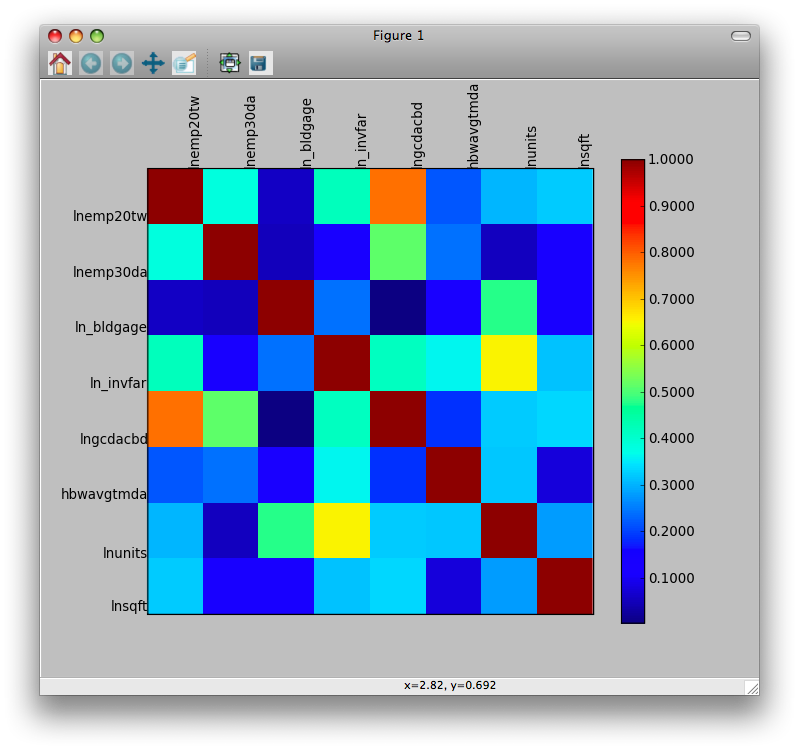
\includegraphics[scale=0.35]{graphics/correlation30.png}
\end{center}
\caption{Correlation Matrix Plot for Submodel 30 in Real Estate Price Modell}
\label{fig:correlation30}
\end{figure}

Note that when a plot is generated from the command line in
Python, control of Python is focused on the graphics window,
and there is no Python prompt available.  When finished
viewing the figure, exit the graphics window by clicking on
the x to close it, and the Python prompt will return for
more interactive commands.

We can retrieve the data for submodel 30 as a dataset that
we can further analyze using Opus methods for the Dataset
class.  Begin with the following command to retrieve the
data and assign it to an object called ds30 (for submodel
30):

\begin{verbatim}
>>> ds30 = estimator.get_data_as_dataset(30)
\end{verbatim}

The syntax above indicates that we are executing a method
called get\_data\_as\_dataset of the class estimator, which
is the class that is running the estimation of the model.
The value 30 in parentheses is an argument being passed to
this method, to identify that we want to retrieve only the
subset of the data that corresponds with submodel 30.  If we
wanted all the data, we would leave out the argument, but
keep the empty parentheses.  Note that nothing special
happens when this command is executed.  If it succeeded, it
will create the new dataset object called ds30, and return
to the python prompt.  At this point, we can use a variety
of built in methods for the dataset class to further explore
the data.  The first of these methods is summary(), which
computes a statistical summary of the data in this object,
like so:
\\

\begin{verbatim}
>>> ds30.summary()
Attribute name	    mean	      sd	      sum	    min	    max
-------------------------------------------------------------------
 lnemp20tw	    8.94	    1.61	  4075.61	5.02388		12.2689
hbwavgtmda	   13.15	     1.8	  5995.99	10.1786		18.0341
   lnunits	    1.08	    1.47	  492.089	      0		5.63121
ln_bldgage	    3.08	    1.41	  1404.12 -0.287682		4.60517

Size: 456 records
identifiers:
  id in range 1-456
\end{verbatim}


Another useful Dataset method is the plot\_histogram, which
computes a histogram for an attribute of a dataset and plots
it, as shown in Figure \ref{fig:histogram-lnsqft}:
\\

\begin{verbatim}
>>> ds30.plot_histogram('ln_bldgage')
\end{verbatim}

\begin{figure}[htp]
\begin{center}
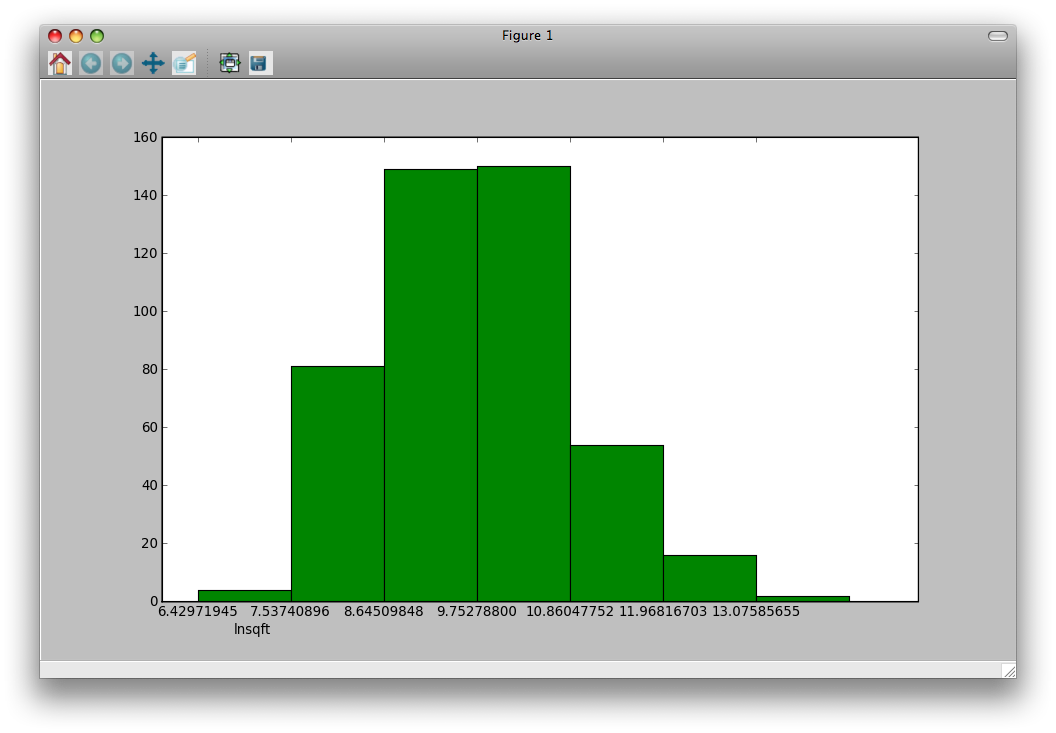
\includegraphics[scale=0.35]{graphics/histogram-lnsqft.png}
\end{center}
\caption{Histogram of Lnsqft from Data in Submodel 30 of the Real Estate Price Modell}
\label{fig:histogram-lnsqft}
\end{figure}

After interactive exploration of the data used in the model,
we might choose to drop or add variables from the
specification.  For demonstration purposes, drop lnemp30da
from the specification of submodel 30, in the GUI, and save
the project.  Alternatively this could be done by editing
the seattle\_parcel.xml (be careful to use an editor that
will not damage the format of the file, for example in
Windows you can use a Notepad version that has added XML
support). Once the specification has been edited and saved,
re-run the estimation for only submodel 30 like this:
\\

\begin{verbatim}
>>> estimator.reestimate(30)
Estimating Real Estate Price Model (from urbansim.models.real_estate_price_model): 
started on Thu May 22 09:36:12 2008
    Estimate regression for submodel 30
    Number of observations: 456
    WARNING: Estimation may led to singularities. Results may be not correct.
    R-Squared:             0.23563241597137002
    Adjusted R-Squared:    0.22368917247092268
    Suggested |t-value| >  2.4743671533372704
    -----------------------------------------------
    Coeff_names estimate        SE      t-values
      constant   7.69055         0.83843         9.17256
    hbwavgtmda  -0.0395769      0.0164105       -2.41168
    ln_bldgage  -0.0340862      0.0220738       -1.54419
     ln_invfar   0.26758        0.0346613        7.71983
     lnemp20tw  -0.030372       0.0279526       -1.08655
     lngcdacbd  -0.545171       0.200477        -2.71937
        lnsqft  -0.118709       0.0256177       -4.63389
       lnunits  0.204933        0.0268876        7.62182
    ===============================================

Estimating Real Estate Price Model (from urbansim.models.real_estate_price_model): 
completed...0.1 sec
\end{verbatim}

Notice that now we see a warning, indicating a problem in
the specification.  Let's drop the least significant
variable, lnemp20tw, and try estimating again:

\begin{verbatim}
>>> estimator.reestimate(30)
Estimating Real Estate Price Model (from urbansim.models.real_estate_price_model): 
started on Thu May 22 09:43:26 2008
    Estimate regression for submodel 30
    Number of observations: 456
    R-Squared:             0.23361810689099238
    Adjusted R-Squared:    0.22337692346414595
    Suggested |t-value| >  2.4743671533372704
    -----------------------------------------------
    Coeff_names estimate        SE      t-values
      constant   6.99788        0.544696         12.8473
    hbwavgtmda  -0.0378939      0.0163405       -2.31901
    ln_bldgage  -0.037881       0.0218001       -1.73765
     ln_invfar  0.271372        0.0344921        7.86765
     lngcdacbd  -0.390517       0.141209        -2.76553
        lnsqft  -0.121596       0.0254847       -4.77133
       lnunits  0.203752        0.0268711        7.58258
    ===============================================
\end{verbatim}

Now the results do not indicate a warning, though we could
experiment further to refine the specification. This
interactive approach is very efficient for rapidly
experimenting with model specifications and re-estimating a
single model.  The same approach is available to estimate a
subset of the models, using the following syntax:

\begin{verbatim}
>>> estimator.reestimate(submodels=[3,7,9])
\end{verbatim}

\subsection{Estimation of a Choice Model}

From the command shell (but not in python), we can also
start the estimation of a choice model, like the housing
type choice model created earlier in this chapter:

\begin{verbatim}
python -i c:\opus\src\urbansim\tools\start_estimation.py 
-x c:\opus\project_configs\seattle_parcel.xml -m housing_type_choice_model 
\end{verbatim}
(Put this command in one single line or with proper continuation
mark for respective operation system.)

The resulting output is shown below:

\begin{verbatim}
(clipped listing)
...
Estimating Choice Model (from opus_core.choice_model): started on Thu May 22 09:51:57 2008
    single_family=(household.disaggregate(building.building_type_id)==19)+1....0.3 sec
    submodel: -2
    Convergence achieved.
    Akaike's Information Criterion (AIC):  333880.22475104179
    Number of Iterations:  18
    ***********************************************
    Log-likelihood is:            -166938.1123755209
    Null Log-likelihood is:       -177492.11908410664
    Likelihood ratio index:       0.059461832801627756
    Adj. likelihood ratio index:  0.059450564695695318
    Number of observations:       256067
    Suggested |t-value| >         3.5289083875852207
    Convergence statistic is:     0.00048567907076085262
    -----------------------------------------------
    Coeff_names     estimate        std err         t-values
      constant      0.600053        0.00561164        106.93
        income      1.13913e-05     5.77362e-08      197.299
    ***********************************************
    Elapsed time:  11.355681 seconds
Estimating Choice Model (from opus_core.choice_model): completed...12.5 sec
\end{verbatim}

Note that the same method used for the regression model,
get\_data\_as\_dataset, can be used to retrieve the data and
analyze it interactively.

There are additional tools in the estimator provides help
for exploring and analyzing the data and model:
\begin{itemize}
%\item plot_choice_set
%\begin{verbatim}
%## plot the alternatives, and its attribute in the alternative set 
%>>> estimator.plot_choice_set()
%>>> estimator.plot_choice_set_attribute('ln(gridcell.residential_units)')
%\end{verbatim}
\item plot_utility helps reveal the relative influence of
  each variable on the utility of the choice model. After
  replacing the estimation procedure of the choice model
  ``bhhh_mnl_estimation'' with
  ``bhhh_mnl_estimation_with_diagnose'' in the
  configuration, enter the interactive estimation mode as
  shown above, then in the Python shell
\begin{verbatim}
>>> estimator.plot_utility()
\end{verbatim}
\item prediction_success_table provides a way to do
  in-sample validation, by applying the estimated
  coefficients to the estimate data to get predicted choices
  and comparing these choices to the observed ones.
\begin{verbatim}
>>> estimator.create_prediction_success_table()
\end{verbatim}
  For location choice model, for example, Household Location
  Choice Model, where there are too many alternatives for
  this to be useful, a summary topology can be provided:
\begin{verbatim}
>>> estimator.create_prediction_success_table(summarize_by= \
    "building_type_id=building.building_type_id")
>>> estimator.create_prediction_success_table(summarize_by= \
    "large_area_id = household.disaggregate(faz.large_area_id, \
    intermediates = [zone, parcel, building])")
# log output to a tab delimited file
>>> estimator.create_prediction_success_table(summarize_by= \
    "area_type_id=building.disaggregate(zone.area_type_id, \
    intermediates=[parcel])",log_to_file='a.out')
\end{verbatim}

\end{itemize}
\chapter{Creating Synthetic Households for OPUS Modeling Applications}

UrbanSim and other models such as activity-based travel model are microsimulation models that simulate the choices of individual households and persons.  In order to operationalize such models, a synthetic household population is needed.  Although there are now several household synthesizers in existence and use, it was deemed important to tightly integrate a household synthesizer into OPSUS in order to support UrbanSim and activity-based travel modeling within the OPUS environment.

A new household synthesizer has been developed and contributed to the OPUS user community through a collaboration with Ram Pendyala and Karthik Konduri at Arizona State University.  A paper submitted for presentation to TRB 2010 describes the algorithm and results on a test application. The paper is \emph{A methodology to match distributions of both household and person attributes in the generation of synthetic populations}, by Xin Ye, Karthic Konduri, Ram Pendyala, Bhargava Sana, and Paul Waddell. 

The UrbanSim group at UW has begun the process of fully integrating the synthesizer into OPUS, by adding an interface in the GUI, and adding supporting tools to create the inputs for the synthesizer, and to post process outputs from the synthesizer.  The synthesizer uses inputs from the U.S. Census by census block group, and from the Public Use Microdata sample.  Tools have been coded to create these inputs from standard census data files, and to set up and launch the synthesizer.  These tools are visible in the tools section of the data tab in the GUI.  They are now in testable condition but have not been extensively tested.

The synthesizer creates a household table and a persons table, with categories for several characteristics and a geographic identifier of a census block group.  Post-processing tools allow the imputation of point values for catergorical characteristics such as income, and also for assigning synthetic households to specific buildings.  The latter step is currently being integrated into the GUI, and depends on having an estimated household location choice model, since this model is used to place the households that are assigned to a block group into a specific building.

The table below provides an example of the household and person characteristics used in the initial development and testing of the synthesizer.  See the paper for details of the algorithm and for validation results.

\begin{centering}
\begin{tabular}{p{2in}ll}
%\hline
\textbf{Household Attributes} & \textbf{Description} & \textbf{Value} \\
\hline
Household Type	& Family: Married Couple	& 1\\ %\hline
&	Family: Male Householder, No Wife &	2 \\ %\hline
&	Family: Female Householder, No Husband & 3 \\ %\hline
&	Non-family: Householder Alone	& 4 \\ %\hline
&	Non-family: Householder Not Alone	& 5 \\ \hline
Household Size &	1 Person	& 1 \\ %\hline
&	2 Persons	 & 2\\ %\hline
&	3 Persons	& 3 \\ %\hline 
&	4 Persons	& 4 \\ %\hline
&	5 Persons &	5 \\ %\hline
&	6 Persons	& 6  \\ %\hline
&	7 or more Persons & 7 \\ \hline
Household Income	& \$0 - \$14,999 &	1\\ %\hline
&	\$15,000 - \$24,999  &	2\\ %\hline
&	\$25,000 - \$34,999 &	3\\ %\hline
&	\$35,000 - \$44,999 &	4\\ %\hline
&	\$45,000 - \$59,999 &	5\\ %\hline
&	\$60,000 - \$99,999 	& 6\\ %\hline
&	\$100,000 - \$149,999 & 7\\ %\hline
&	Over \$150,000 &	8\\ %\hline
\textbf{Person attributes}		& & \\ \hline
Gender	& Male	& 1\\ %\hline
&	Female	& 2\\ \hline
Age	& Under 5 years	& 1\\ %\hline
&	5 to 14 years	& 2\\ %\hline
&	15 to 24 years	& 3\\ %\hline
&	25 to 34 years	& 4\\ %\hline
&	35 to 44 years	& 5\\ %\hline
&	45 to 54 years	& 6\\ %\hline
&	55 to 64 years	& 7\\ %\hline
&	65 to 74 years	& 8\\ %\hline
&	75 to 84 years	& 9\\ %\hline
&	85 and more	 & 10\\ \hline
Ethnicity &	White alone	& 1\\ %\hline
&	Black or African American alone	& 2\\ %\hline
&	American Indian and Alask Native alone	& 3\\ %\hline
&	Asian alone	& 4\\ %\hline
&	Native Hawaiian and Other Pacific Islander alone &	5\\ %\hline
&	Some other race alone	& 6\\ %\hline
&	Two or more races	& 7\\ \hline
\end{tabular}
\end{centering}



%% Copyright (c) 2005-2008 Center for Urban Simulation and Policy Analysis,
% University of Washington.  Permission is granted to copy, distribute and/or
% modify this document under the terms of the GNU Free Documentation License,
% Version 1.2 or any later version published by the Free Software Foundation;
% with no Invariant Sections, no Front-Cover Texts, and no Back-Cover Texts.
% A copy of the license is included in the section entitled "GNU Free
% Documentation License".

\chapter{Using the UrbanSim System}
\label{chapter:using-urbansim}
%
The latest incarnation of UrbanSim, UrbanSim 4, is implemented as a
set of packages in Opus. Package \package{opus_core} provides
general functionality, \package{urbansim} contains everything around
land use models, \modelsindex package \package{opus_emme2} is an
Opus wrapper to the travel model EMME/2.\emmeindex

\section{Running a Simulation}
%
\subsection{Support for Production Runs}
The ``Run Manager'' \runmanagerindex is a set of user functionality
provided by the \file{run_manager} \runmanagerindex directories in
the \package{opus_core} and \package{opus_core.services} packages
provide support for specifying, starting, re-starting, and
processing ``production`` runs. \index{production runs} Such a
system is necessary to deal with the long run times for such a model
\modelsindex system, and the large amount of data each run produces.
A 30-year simulation of the Puget Sound Regional Council's (PSRC)
\psrcindex dataset with their EMME/2 \emmeindex travel model, for
instance, takes about 5 days \index{simulation!run time} to complete
and creates about 14 GB of cache data. \index{cache!size of}
\index{simulation!space used by}  These numbers are for a computer
with dual 3.2 GHz Intel\textregistered{} \intelindex
Xeon\texttrademark{} \xeonindex processors and 4 GB of RAM running
Windows XP Professional. \windowstestindex  The PSCS dataset
\datasetindex contains about 800,000 gridcells, 1.3 million
households, and 1.8 million jobs in the initial year. Each UrbanSim
year takes about 1.5 hours to simulate, and each travel model run,
done every 5 years, takes around 12 hours to simulate.

Here are some of the things Run Manager \runmanagerindex helps us do:
\begin{itemize}
  \item Define a run configuration, including what models \modelsindex to run, what years to
  run, etc.
  \item Start a production run.
  \item Monitor the status of all production runs.
  \item Re-start a production run when something goes wrong.
  \item Compute indicators on the results of a production run, including runs
  that are still simulating.
  \item Inspecting specific dataset values from any year of the simulation,
  as when diagnosing problems.
  \item Manage consistency regarding the availability and status of production runs.
\end{itemize}

\subsection{Run Management}
\label{sec:run-manager}
%
Opus contains a set of scripts that simplify the
process of starting and restarting a set of simulation runs.

At the moment, these scripts are a set of command line applications, or tools, in the
\file{opus_core/tools} directory.  They use a database as the central
repository for coordination and context infomation for run managment, by
default called \verb|services|.  If you don't have this database, create it
(you need to do this from within the \file{opus_core/tools}
directory):
\pythonindex
\begin{verbatim}
python create_services_database.py
\end{verbatim}
This creates the database named \verb|services| on the \verb|localhost|
database server using the user name and password specified in the
\verb|MYSQLUSERNAME| \mysqlusernameindex and \verb|MYSQLPASSWORD| \mysqlpasswordindex environment variables. \environmentvariablesindex To use a
different host for the database server, include the \verb|--hostname|
option. To use a different database name, include the \verb|--database|
option:
\pythonindex
\begin{verbatim}
python create_services_database.py --hostname myhost.mydomain --database
myservices
\end{verbatim}

All scripts described below print a help message when called with the
\verb|-h| or \verb|--help| option.

\subsubsection{Start a simulation using a Python Dictionary Configuration}
\index{start a simulation}

The configuration for a simulation is specified by a configuration object.
Previously, a configuration was specified as a Python dictionary, and we
describe the older option in this section.  We are transitioning toward
specifying configurations using an xml project file for use with the Opus
GUI--- see Section \ref{sec:start-simulation-xml} for information on
starting a simulation using an xml configuration but still from the command
line.  In both cases, the configuration is used to specify different parts
of the simulation, such as the years in which to run UrbanSim, what
UrbanSim models \modelsindex to run each year, what types of development
projects exist, how to configure each type of development project,
etc. See, for instance, the run configuration in
\verb|seattle_parcel/configs/baseline.py| (Python dictionary version) or
\verb|seattle_parcel/configs/seattle_parcel.xml| (xml version).

To use the dictionary version of a configuration, the start_run tool
requires that the referenced configuration Python module either (a) defines
a class (e.g. SubsetConfiguration) in a file whose name is
subset_configuration.py, or (b) defines a run_configuration object that is
the configuration object.  In the first case, the class name is the
CamelCase version of the lowercase_with_underscores file name.  \emph{(The
  preferred method is to define a class.)}

To start a simulation using a dictionary-based configuration, use the
script \verb|start_run| with the desired configuration.  First change to 
the directory \verb|opus_core/tools| and execute:
\begin{verbatim}
python start_run.py -c psrc.configs.subset_configuration
\end{verbatim}

Note that the configuration here is specified as it would be in a Python
``import'' statement.

If the \verb|services| database was created using the \verb|--hostname| and/or
\verb|--database| option, you will need to include these options in
\file{start_run.py} as well.  Use the \verb|--help| option to see
\verb|start_run|'s possible command line parameters.

The \verb|creating_baseyear_cache_configuration| entry in the configuration
contains the information specifying the location of the baseyear inputs.  
If \verb|cache_from_mysql| is \verb|True|, the inputs are taken from
the MySQL database specified in the \verb|input_configuration| entry. 
Otherwise, the inputs are taken from the baseyear cache specified in the
\verb|baseyear_cache| entry.  When the inputs are taken from MySQL, they are
used to create a baseyear cache stored in the directory specified by the
\verb|cache_directory| entry, or, if that entry is missing, from an directory
whose name encodes the date-time of the simulation request and is created in the
directory specified by the \verb|cache_directory_root| entry.  

For large amount of data, copying from MySQL to a baseyear cache takes much
longer than creating a new baseyear cache from an existing baseyear cache.  

Option \verb|--directory-to-cache| \index{cache!getting input from existing cache}
can be used to turn off the caching. It takes as argument the directory name
from which data are copied to the new basyear cache \baseyearcacheindex. With
the option \verb|--years-to-cache| one can control specific years to be
copied. The option takes as argument any python \pythonindex expression that returns a list
of years. These two options overwrite entries in the configuration that control
this behaviour.

\subsubsection{Start a simulation using an XML Configuration}
\label{sec:start-simulation-xml}

To start a simulation using an xml configuration from the command line, use
the script \verb|start_run| with the desired configuration.  Change to the
directory that holds the Opus source code and execute:
\begin{verbatim}
python opus_core/tools/start_run.py -x seattle_parcel/configs/seattle_parcel.xml 
       -s Seattle_baseline
\end{verbatim}
(typed all on one line).

Notice that the \verb|-x| option takes a path to the file with the xml
configuration.  Since xml configurations can hold multiple scenarios, the
scenario name must also be specified using the \verb|-s| option.

This same xml configuration can also be used with the Opus GUI ---
documentation on the GUI is forthcoming.

\subsubsection{Restart a simulation}
\index{restart a simulation}
If you halt a run or it fails, you can restart it at the beginning of any year.
To restart the run with \verb|run_id| 42 at the beginning of year 2005, do:
\pythonindex
\begin{verbatim}
python restart_run.py 42 2005
\end{verbatim}
Again, options \verb|--hostname| and \verb|--database| must be included
if non-default values are used.  Note that the above command will delete any
simulation cache \simulationcacheindex directories for years 2005 onward, since
this information is no longer valid once the simulation is restarted at the
beginning of 2005.

If the 2005 travel model failed and you want to restart in 2005 but not re-run
the UrbanSim models, \modelsindex use the \verb|--skip-urbansim| option:
\pythonindex
\begin{verbatim}
python restart_run.py 42 2005 --skip-urbansim
\end{verbatim}

If the 2005 travel model succeeded, and thus wrote its output to the 2006
simulation cache \simulationcacheindex directory, but you need to restart in year 2006, use the
\verb|--skip-cache-cleanup| option:
\pythonindex
\begin{verbatim}
python restart_run.py 42 2006 --skip-cache-cleanup
\end{verbatim}

\subsubsection{Create Baseyear Cache}
\label{sec:run-manager-baseyearcache}
%
One can explicitely create a baseyear
cache \baseyearcacheindex\index{cache!getting input from existing cache} from
the base year database which can be then used for simulation runs. The script
needs a configuration module passed as an argument. The services database is
not used by the script. If the desired module is located at
\file{psrc/configs/subset_configuration.py} under one of the paths found in the
PYTHONPATH \pythonpathindex environment variable, \environmentvariablesindex the command
\pythonindex
\begin{verbatim}
python create_baseyear_cache.py psrc.configs.subset_configuration
\end{verbatim}
caches the database defined in the \verb|subset_configuration| configuration into a basyear
cache. \baseyearcacheindex The \file{create_baseyear_cache} file is located in
the \file{opus_core/tools/} directory, and the above command should be
run from the same directory. An option \verb|--cache-directory|
can be used to pass the directory to be cached into. Alternatively, this can be
specified in the configuration as an entry \verb|'cache_directory'|. See also
Section~\ref{sec:configuration} for configuration and cache control options.

\subsection{What Happens When Running a Simulation?}
\label{sec:run-manager-tasks}
Here are the steps that occur when you start a run via the \verb|start_run|
script:

\begin{itemize}
  
\item \index{cache!unrolling development_event_history}\index{Unrolling 
development_event_history}\index{development_event_history!unrolling} If 
required, it copies all of the tables from the baseyear database specified by 
the configuration into the baseyear cache \baseyearcacheindex and then creates a
set of pre-baseyear \verb|gridcells| tables by unrolling the
\verb|develoment_event_history| data.

The unrolling processes all records in the \verb|development_event_history| 
table.  It starts with the most current year of records, and moves backward in 
time.  For this description, assume that the baseyear is 2000.  The unrolling 
process first loads the gridcell dataset for year 2000.  For each 
\verb|develoment_event_history| record with \verb|scheduled_year| for the prior 
year (e.g. for 1999) it substracts from the gridcells any development by that 
event (e.g. \verb|residential_units|).  Values that go negative are set to 
zero.  Once all events for this year have been ``undone'', the unrolling 
process writes the modified gridcell dataset to the prior year, e.g. to 1999. 
This process is repreated for each year with data in 
\verb|develoment_event_history|.

If you only want 10 years of data to be unrolled, only put those years of data
into your \verb|develoment_event_history| table.

\item Alternatively, it copies files from a previously used baseyear cache into
the baseyear cache for the current run (including the

\item It adds a row to the \verb|run_activity| table in the \verb|services|
database, using a new \verb|run_id| value unique to this run. In order to help
match runs with their cache directory, the name of the cache directory begins
with the \verb|run_id| value, e.g. \file{run_342.2006_04_25_09_40}.

\item For each year in the set of years specified in the configuration:
  \begin{itemize}
  \item Stores to the cache a pickled version of the configurations for that
  year.
  \item Forks a new process to run the set of UrbanSim models \modelsindex for this year.
  The set of models \modelsindex to be run is specified by the configuration. Using a
  separate process helps reduce memory usage, \index{Memory!Using separate
  process} and helps reduce the impact of problems such as memory leaks.  This
  process writes a log file named, e.g., \file{year_2003_log.txt}.
  \item Run the EMME/2 \emmeindex travel model for this year, if specified by the travel
  model's configuration.  The set of steps to run for the travel model is fully
  specified by the \verb|'models'| \modelsindex section of the
  \verb|'travel_model_configuration'|. Typically, it includes a preparation step
  that prepares travel model inputs from the UrbanSim data, a step that
  actually runs the travel model, and one or more steps to puts the results of
  the travel model into the \verb|travel_data| dataset for the current year, so
  the data is visible to the UrbanSim models \modelsindex in that and following years.  Each
  model step is done in a separate process.  The log for the running of the
  model is written to a file named, e.g., \file{emme2_2005_log.txt}. \emmeindex
  \end{itemize}
  \item The run activity table includes status information about the run.  If
  the simulation succeeds, it will add another row to the run activity
  indicating it is done.  If the simulation fails, it will add a row indicating
  that.  The run activity also contains a copy of the configuration, which is
  used when restarting a run.
  \item Whenever a row is added to the \verb|run_activity| table, a row is
  either added or updated in the \verb|available_runs| table in the
  \verb|services| database. This table has a single row per run and records the
  row's current state and information.
\end{itemize}

\section{Configurations}
\label{sec:configuration}
%
A run configuration is a specification of what parts to use in the simulation
and how to configure each part.  Parts include the list and order of models \modelsindex to
run, where to get the input values, where to store the output data, what years
to simulate, what tables to store into the UrbanSim baseyear and simulation
caches \baseyearcacheindex\simulationcacheindex, etc. Each of these parts in
turn may be configurable.  The configuration for a travel model, for instance,
may specify which values to use from the land use models, \modelsindex and what travel model
results to extract in order to use them in the land use models. \modelsindex

Configurations are used in many places in Opus.  Typically, they are specified
via a Python \pythonindex dictionary that then is used to create an instance of the
\class{Configuration} class.

\subsection{Run Manager Configuration}
\label{sec:run-manager-configuration}
%

UrbanSim can be started via the ``Run Manager'' \runmanagerindex (see
Section~\ref{sec:run-manager}) which is controlled by a user-defined
configuration. The following code contains a fully specified configuration
that influences behaviour of the run manager. \runmanagerindex Mandatory entries and default
values for optional entries are marked in the comments. The actual values for
the listed entries are only examples.

\emph{Note: we are in the process of splitting the following configuration
information into separate parts.  Once we are done with that refactoring,
we will update the documentation to the new arrangement.}

\mysqlhostnameindex\mysqlpasswordindex\baseyearcacheindex
\begin{verbatim}
from opus_core.configurations.database_configuration import DatabaseConfiguration
from opus_core.configurations.baseyear_cache_configuration \
    import BaseyearCacheConfiguration
    
from urbansim.configurations.creating_baseyear_cache_configuration \
    import CreatingBaseyearCacheConfiguration


run_configuration = {
    'model_system':'urbansim.model_coordinators.model_system', # mandatory
    'description':'baseline with travel model',      # default: 'No description'
    'cache_directory':'d:/urbansim_cache/',	         # mandatory
    'creating_baseyear_cache_configuration': CreatingBaseyearCacheConfiguration(
        # default: 'urbansim_tmp'+random string
        cache_directory_root = 'd:/urbansim_cache',

        # mandatory
        cache_scenario_database = 'urbansim.model_coordinators.cache_scenario_database',

        cache_from_mysql = False, # default: True

        # mandatory if 'cache_from_mysql' is False
        baseyear_cache = BaseyearCacheConfiguration(
            # mandatory for this block
            existing_cache_to_copy = 'd:/urbansim_cache/run_397.2006_05_23_18_21',
            
            # default: all years in 'existing_cache_to_copy'
            years_to_cache = range(1996,2001)
            },

        tables_to_cache = [ # default: []
            'gridcells',
            'households',
            'jobs',
            'zones'
            ]

        tables_to_cache_nchunks = { # default: each table defaults to 1
            'gridcells':2,
            },

        tables_to_copy_to_previous_years = { # default: no copied tables
            'development_type_groups':1996, # table name and year to put it in
            'development_types':1996,
            'development_type_group_definitions':1996,
            'urbansim_constants': 1996,
            },
        ),
\end{verbatim}

% long script split into two parts since it won't fit on one page

\begin{verbatim}
    'input_configuration': DatabaseConfiguration(    # mandatory
        host_name = os.environ['MYSQLHOSTNAME']      # mandatory
        user_name = 'urbansim',                      # mandatory
        password = os.environ['MYSQLPASSWORD'],      # mandatory
        database_name = 'PSRC_2000_baseyear',        # mandatory
        )
    'output_configuration': DatabaseConfiguration(   # default: No output
                                                     #     configuration
        host_name = os.environ['MYSQLHOSTNAME']      # mandatory for this block
        user_name = 'urbansim',                      # mandatory for this block
        password = os.environ['MYSQLPASSWORD'],      # mandatory for this block
        database_name = 'PSRC_2000_output',          # mandatory for this block
        },
    'base_year': 2000,                               # default: read from table
                                                     #     'base_year' in
                                                     #     'db_input_database'
    'years': (2001, 2030),                           # mandatory
}
\end{verbatim}
The \verb|'model_system'| entry is the full Opus path to the model system that
will be used by the run manager to run/estimate a set of models.

The \verb|'cache_scenario_database'| entry is the full Opus path to the class to use to
create a baseyear cache from the baseyear data in the MySQL database.  The
\verb|'urbansim.model_coordinators.cache_scenario_database'| version creates  both the
baseyear cache, and unrolls the gridcell data to populate prior years with the
gridcell dataset (see Section~\ref{sec:run-manager-tasks}).

Entry \verb|'creating_baseyear_cache_configuration'| contains the configuration
for creating the baseyear cache.

Entry \verb|'cache_directory_root'| is the root directory where data should be
cached during processing. The actual cache directory is created by adding
the run number and date-time string to this directory.

The \verb|'input_configuration'| is a DatabaseConfiguration object
that determines the MySQL \mysqlindex database with the base year
data.

Entry \verb|'output_configuration'| is a DatabaseConfiguration
object that determines the MySQL \mysqlindex database into to which
to write any database tables related to the results of the
simulation run.  Now that indicators are computed from the attribute
cache, the output database is only needed if you wish to use the SQL
indicators.  Before starting the simulation, the run manager will
remove any tables in the output_database, so be sure it doesn't
contain information you want to keep.

Entry \verb|'years'| determines for what
years the simulation should run as a tuple with first and last year to run.

By default, the run manager \runmanagerindex caches all tables from the input database into the
binary baseyear cache \baseyearcacheindex on which then the simulation runs. If
only selected tables should be cached, they can be put into
\verb|'tables_to_cache'|. Note that the simulation itself then does not use the
database anymore, all data are retreived from baseyear cache \baseyearcacheindex
and written to the simulation cache \simulationcacheindex.  That means, if the
entry \verb|'tables_to_cache'| is used, the user must ensure that it contains
all tables that are used by the simulation.

If a database table is so large that Python \pythonindex runs out of memory when copying it
to cache, you can reduce memory usage (but increase the time it takes to cache
the data) by increasing the number of ``chunks'' in which the dataset's \datasetindex
attributes are read from the table. \index{Memory management!When caching data
from input store}\index{Memory management!tables_to_cache_nchunks@\texttt{tables_to_cache_nchunks}} By
default, all attributes of a table are read in a single chunk. Setting the
\verb|'tables_to_cache_nchunks'| configuration for a model will tell the caching code
to use that many chunks.  For instance, if a dataset has 11 attributes, setting
\verb|'tables_to_chunk_nchunks'| to 3 will use three chunks loading 4, 4, and 3
attributes, in each chunk.

For big tables, the caching process can be a very time-consuming task. Often
the baseyear cache \baseyearcacheindex is available from previous runs. Thus,
one can set the entry \verb|'cache_from_mysql'| \mysqlindex to False and define the
\verb|'baseyear_cache'| \baseyearcacheindex block. The directory with the already cached data
should be put into the entry \verb|existing_cache_to_copy|. The run manager \runmanagerindex then
copies data from that directory into the baseyear cache \baseyearcacheindex for this run. If you
want to copy only selected years, they can be specified in the entry
\verb|years_to_cache| as a list of those years; by default all years are
copied. Note that this behaviour can be alternatively controlled directly from
the command line (see description of \verb|start_run| in~\ref{sec:run-manager})
which has priority over entries in this configuration.

The \verb|'tables_to_copy_to_previous_years'| entry is used when a
lag variable needs to compute data for before the base year, and that
computation requires some of the "invariant" data that was copied from the
baseyear database into the baseyear cache.  If this is the case, add those
database tables to the list of tables in the configuration's
\verb|'tables_to_copy_to_previous_years'| entry, and indicate the year to which
to copy the tables.  In general, it is safe to copy the tables to the earliest
year created by the unroll gridcell process.  You can determine what this year
is by examining the year directories created in your baseyear cache.
\emph{(Note: we plan to change this to a better design.)}

There are several run manager \runmanagerindex configurations in Opus. See for example the
directory \file{psrc/configs} for configuration of different PSRC \psrcindex runs.

\subsection{Model System Configuration}
\label{sec:model-system-configuration}
%
If one would pass the above configuration to the run manager, \runmanagerindex it would perform
steps as described in Section~\ref{sec:run-manager-tasks}, but no models \modelsindex would
be run. The configuration should in addition contain entries that control what
models, \modelsindex in what order and with what input and output should be run. It
determines the behaviour of the class \class{ModelSystem}. UrbanSim basic
configuration of the model \modelsindex system can be found in the file
\file{urbansim/configs/general_configuration.py} as an example.

The set of models \modelsindex to run is specified by the entry ``models''. \modelsindex It is a list of
user-defined model names. The order in this list also specifies the order in
which they are run. A production run of UrbanSim consists by default of
following models: \modelsindex
\begin{verbatim}
run_configuration['models'] = [
        "prescheduled_events",
        "events_coordinator",
        "residential_land_share_model",
        "land_price_model",
        "development_project_transition_model",
        "residential_development_project_location_choice_model",
        "commercial_development_project_location_choice_model",
        "industrial_development_project_location_choice_model",
        "development_event_transition_model",
        "events_coordinator",
        "residential_land_share_model",
        "household_transition_model",
        "employment_transition_model",
        "household_relocation_model",
        "household_location_choice_model",
        "employment_relocation_model", 
       {"employment_location_choice_model": {"group_members": "_all_"}},
        "distribute_unplaced_jobs_model"
   ]
\end{verbatim}
Note that the list can contain a particular model multiple times if that model should
run multiple times within one year, such as the ``events_coordinator'' or
``residential_land_share_model'' in the above list.

We can also define a situation when the same model should be run on different subsets of 
a dataset, so called model group\index{model group}. Then we can give the names of the group members to be run, or 
just configure the model group to be run on all subsets. This is the case of ``employment_location_choice_model''
in the list above (see Section~\ref{sec:model-controller-configuration} for further details).
 
By default, the \class{ModelSystem} runs the method
\method{run()} of the listed models. \modelsindex Each entry in this model list can be
alternatively a dictionary containing one entry: The name of the entry is the model
name, the value is a list of model methods to be processed. Thus, one can combine
estimation and simulation of different models. \modelsindex

In addition (or alternatively), the configuration can contain an entry
``models_in_year''. \modelsindex It is a dictionary where keys are years. Each value is
expected to be such list of models \modelsindex as above. In each year, it is checked if
``models_in_year'' \modelsindex (if it is present) contains that year. If it is the case,
its list of models \modelsindex is run, instead of the global set of models. \modelsindex This allows
users to set different set of models \modelsindex for different years, for example an
additional model can be run only in the first year, or last year.

For each entry in the model \modelsindex lists above there must be a corresponding entry in
the ``controller'' configuration which specifies how models \modelsindex are initialized,
what methods to run and what arguments should be passed in. This will be
described in Section~\ref{sec:model-controller-configuration}.

Furthermore, the configuration can contain the following entries (the given
values are defaults set by our system):
\begin{verbatim}
{
    'datasets_to_cache_after_each_model':[],
    'flush_variables': False,
    'seed':0,
    'debuglevel':0
}
\end{verbatim}

The entry \verb|'datasets_to_cache_after_each_model'| specifies names of datasets \datasetindex that
are flushed from memory to simulation cache \simulationcacheindex at the end of each model
run. \index{Memory management!Flushing attributes}\index{Memory management!datasets_to_cache_after_each_model@\texttt{datasets_to_cache_after_each_model}} This reduces the memory
usage, but can increase the run time. We recommend to put datasets in this list
that contain huge amount of data. E.g. UrbanSim sets this entry to ['gridcell',
'household', 'job'].

\verb|'flush_variables'| can further decrease the memory usage. \index{Memory management!flush_variables@\texttt{flush_variables}} If it is True, after each variable
computation all dependent variables are flushed to simulation
cache \simulationcacheindex, regardless to what dataset \datasetindex the variables belong to.
Nevertheless, it increases the run-time considerably.

Entry \verb|'seed'| specifies the seed of the random number generator that is set at
the beginning of each simulated year. It is passed to the \module{numpy} \numpyindex
function \method{seed()} and therefore it should be a tuple with two integer
values. If both values are 0, the function generates a pseudo-random seed
from the current time.

\verb|'debuglevel'| controls the amount of output information.

Models \modelsindex usually need various datasets \datasetindex to run with. They are specified in the
configuration entry \verb|'datasets_to_preload'|. For example,
\begin{verbatim}
{
'datasets_to_preload': {
        'gridcell':{"id_name": "grid_id"},
        'household':{}
}
\end{verbatim}
It is a dictionary that has dataset \datasetindex names as keys. Each value is again a
dictionary with argument-value pairs that are passed to the corresponding
dataset \datasetindex constructor. \class{ModelSystem} \modelsindex creates those datasets \datasetindex at the
beginning of each simulated year and they are accessible to the models \modelsindex
definition in the controller through their names (see
Section~\ref{sec:model-controller-configuration} for details). One should put
here all datasets \datasetindex that will be passed as arguments to the model constructors
or to the model methods to be processed.

If you do not want to make any output to cache, for example in estimation mode, set
\begin{verbatim}
{
    'low_memory_mode': False
}
\end{verbatim}
This should be only used when you're aware what you're doing.
It suppresses any cache writing during the processing (after each model, as
well as at the end of each year) and will not work for a simulation
over multiple years. Also, the memory usage can increase considerably.


\subsection{Models Configuration}
\label{sec:models-configuration}
%
The run configuration can contain an entry \verb|'models_configuration'| \modelsindex which can
include any information specific to models \modelsindex or common to a set of models. \modelsindex The
value of this entry is a dictionary.  Model specific information would be
included in an entry of the same name as the model name used in the entry
\verb|'models'| (see Section~\ref{sec:model-system-configuration}). The
\class{ModelSystem} \modelsindex class makes this information available to the controller
by creating two local variables: \verb|'models_configuration'| \modelsindex (containing the
value of \verb|'models_configuration'| \modelsindex and available to all models) \modelsindex and
\verb|'model_configuration'| \modelsindex (available to each model at the time of its
processing and containing information for this model). See the variable
\verb|'models_configuration'| \modelsindex in the file \file{urbansim/configs/general_configuration.py} for an
example how UrbanSim configures models. \modelsindex

If a model is running out of memory, you can add a \verb|'chunk_specification'|
to that model's configuration. \index{Memory management!Using multiple chunks per model}
\index{Memory management!chunk_specification@\texttt{chunk_specification}} This instructs that model to run in
multiple chunks, each containing a subset of the records (e.g., agents) to
process. This specification can either limit the chunk to contain at most a
given number of records:

\begin{verbatim}
    'chunk_specification':{
        'records_per_chunk':300,     # Put at most 300 records in a chunk
        per chunk },
\end{verbatim}

or specify the number of chunks to use regardless of the number of records:

\begin{verbatim}
    'chunk_specification':{
        'nchunks':10,                # Use 10 chunks
        },
\end{verbatim}

\subsection{Model Controller Configuration}
\label{sec:model-controller-configuration}
%
Each model that is included in the configuration entry \verb|'models'| \modelsindex must have a
controller entry in the \verb|'models_configuration'| \modelsindex entry described in
Section~\ref{sec:models-configuration}.  More specifically, the model specific
section of \verb|'models_configuration'| \modelsindex is expected to contain an entry \verb|'controller'|
for each model. For example, a controller specification for the model
specified by the name \verb|'land_price_model'| would be contained in\\
\verb|run_configuration['models_configuration']['land_price_model']['controller']|.

If a model is specified as a model group \index{model group} it is possible to define a member specific controller, called 
{\em member_name} + '_' + {\em model_name}, e.g. \verb|'home_based_employment_location_choice_model'|.
When choosing the right controller, the \class{ModelSystem} checks for the member specific name. If it is not found,
it uses the group name, in this example \verb|'employment_location_choice_model'|.

The value of this controller entry is a dictionary with a few well-defined entries:
\begin{description}
\item["import"] A dictionary where keys are module names and values are names
  of classes to be imported.
\item["init"] A dictionary with a mandatory entry "name". Its value is the
  name of the class (or class.method) that creates the model. It can be the
  name of the model class itself.  Or, if the model is created via   a
  method e.g. \method{get_model()} of a class \class{MyModelCreator}, it would be
  given as "MyModelCreator().get_model".

  Optional entry "arguments" specifies arguments to be passed into the
  constructor. It is given as a dictionary of argument names and values. All
  values are given as character strings and are later converted by
  \class{ModelSystem} to python \pythonindex objects. If an argument value is suppose to be
  a character string object, it must be given in double quotes, e.g.
  "'my_string'".
\end{description}
If the model in the 'models' entry of the configuration is specified as model group\index{model group}, the controller must contain 
an entry
\begin{description}
\item["group_by_attribute"] Its value is a tuple of a grouping dataset name and grouping attribute (see Sec.~ref{sec:model-group}).
They define the specific kinds of 
subsets of agents on which this model can be run. This dataset must be contained in the 
\verb|datasets_to_preload| entry of the configuration. For example, in the controller of the 
``employment_location_choice_model'' this entry is
\verb|('job_building_type', 'name')|, since the attribute 'name' of the dataset 'job_building_type' contains the various
building types of jobs for which we want to run the model, i.e. 'commercial', 'governmental', 'industrial' and 'home_based'.
If the 'group_members' entry (of the 'models' entry of the configuration) for this model is equal to '_all_', the model runs 
for all values found in this dataset. The  'group_members' can also be a list specifying explicitely for which types the model 
should be run. 
\end{description}

The \class{ModelSystem} class evaluates the given imports and creates an
instance of the model by processing the \verb|'init'| entry. The remaining entries
below are related to specific methods of the created model instance.  As
mentioned in Section~\ref{sec:model-system-configuration}, models \modelsindex
that are listed in the \verb|'models'| entry of the run configuration can be also
specified using a list of methods to be processed. If the list is not given, a
method \method{run()} is assumed to be the only method to be processed. The
\class{ModelSystem} iterates over the set of methods. It first processes a
``preparation'' method (if required) and then the method itself. For this purpose,
the controller should contain the following entries:

\begin{description}
\item['prepare_for_...'], where \verb|...| is the the method
to be processed, e.g. \verb|'prepare_for_run'| is the method to call to prepare
to run. This configuration entry is a dictionary with an
optional entry \verb|'name'| giving the name of the preparation method. If \verb|'name'| is
missing, the method name is assumed to be the same as this entry name. Optional
entry \verb|'arguments'| specifies arguments of this method (see \verb|'arguments'| in \verb|'init'|
above). Optional entry \verb|'output'| defines the name(s) of the output of this
method.  It can be then used as an input to other methods or models. The entry
\verb|'prepare_for...'| is optional and if it's missing, no preparation procedure is
invoked. There can be as many \verb|'prepare_for...'| entries as there are
methods specified.
\item[{\it procedure}] The procedure name must match to the method names given
in \verb|'models'| (there must be one entry per method), or be called \verb|'run'| if no
methods are specified in \verb|'models'|. It is a dictionary with optional arguments
\verb|'arguments'| and \verb|'output'| (see above).
\end{description}

The entry \verb|'arguments'| in the above items can contain any character
strings that are convertable (using python's \verb|eval()|) to python \pythonindex objects,
including python \pythonindex expressions. They must be objects that are known to the
\class{ModelSystem}, for example datasets \datasetindex that are defined in
\verb|'datasets_to_preload'| (described in
Section~\ref{sec:model-system-configuration}), since those are created prior to
the simulation. They can be called either by the dataset \datasetindex name, or using
\code{datasets['{\it name}']}. Also, the \verb|model_configuration| and
\verb|models_configuration| objects described in
Section~\ref{sec:models-configuration} can be used in \verb|'arguments'|. Other
objects that \class{ModelSystem} provides are \verb|sql_storage|
(\class{Storage} object for the input database), \verb|cache_storage|
(\class{Storage} object for the simulation cache \simulationcacheindex storage
in the simulated year), \verb|base_cache_storage| \baseyearcacheindex (\class{Storage} object for
the baseyear cache \baseyearcacheindex storage in the base year),
\verb|model_resources| (all preloaded datasets as an object of
\class{Resources}), \verb|year| (simulated year), \verb|resources|
(Configuration passed into the simulation), \verb|dataset_pool| (object of class \class{DatasetPool} pointing to the current
dataset pool).  If you are using any class names
as arguments, you need to make sure, that those classes are known to the
\class{ModelSystem}, e.g. by putting the appropriate import statement into the
\verb|'import'| section of the controller.

Here is an example of a controller settings for the land price model in UrbanSim:
\modelsindex\datasetindex
\begin{verbatim}
run_configuration['models_configuration']['land_price_model']['controller'] = {
    "import": {"urbansim.models.corrected_land_price_model":
                                                "CorrectedLandPriceModel",
              },
    "init": {"name": "CorrectedLandPriceModel"},
    "prepare_for_run": {
        "arguments": {"specification_storage": "base_cache_storage",
                      "specification_table": "'land_price_model_specification'",
                      "coefficients_storage": "base_cache_storage",
                      "coefficients_table": "'land_price_model_coefficients'"},
        "output": "(specification, coefficients)"
        },
    "run": {
        "arguments": {"n_simulated_years": "year-resources['base_year']",
                      "specification": "specification",
                      "coefficients":"coefficients",
                      "dataset": "gridcell",
                      "data_objects": "datasets" ,
                      "chunk_specification":"{'nchunks':2}"
                     }
           }
   }
\end{verbatim}
Note on an implementation of model group\index{model group}: A constructor of 
a model group, must take as its first argument an object of class \class{ModelGroupMember} (Sec.~\ref{sec:model-group}). 
The controller should though ignore this argument, since the \class{ModelSystem} automatically takes care of creating this object 
and passing it to the model constructor.

\section{Output}
%
\subsection{The Output Database}

The simulation reads and writes all of its data from the simulation cache.  It 
does not directly read or write to any database. 
If you wish to move data from the simulation cache to a MySQL database, use the
\verb|do_export_cache_to_sql_database.py| tool located in
\file{opus_core/tools}. 

\subsection{File-Based
Cache}\label{cache} \baseyearcacheindex\simulationcacheindex

For a variety of reasons, described below, UrbanSim uses two forms of file-based
caches:
\begin{description}
\item[baseyear cache] \baseyearcacheindex
Stores the attribute values read from the baseyear
database.  This includes data for the base year, and data for years before the
base year (unrolled from data in the baseyear).  This data is not modified
during the simulation.

\item[simulation cache] \simulationcacheindex
Stores the attribute values for datasets used during the simulation.
\end{description}
While the distinction between the read-only baseyear cache \baseyearcacheindex and read-write
simulation cache \simulationcacheindex is useful understanding the system, during simulation both
caches form a single cache that UrbanSim datasets \datasetindex and models \modelsindex mine to gather data
for the current and prior years.

\subsubsection{Reasons to Use Cache}
The UrbanSim simulations run on top of a file-based cache.  The initial reason
for the cache was to improve performance, and has turned out to be very useful for
many features:

\begin{itemize}
  \item The cache is much faster to access than the MySQL \mysqlindex database, at least,
  so using the cache dramatically speeds up our processing.
  \item In many cases, a simulation will require more data than can fit in RAM.
  The simulation cache \simulationcacheindex provides a place to store computed
  or non-computed values so that we only need to keep in memory just enough
  data for the computation at hand. \index{Memory management!Caching data}
  \item Lag variables use the baseyear cache \baseyearcacheindex and simulation
  cache \simulationcacheindex to quickly get data from prior years, often
  without having to re-compute it.
  \item When preparing for a simulation, UrbanSim uses the data from lag tables
  (see~\ref{lag-tables}) in the baseyear to create historical data in the
  baseyear cache \baseyearcacheindex for years before the base year.  This
  allows the simulation to run without any distinction between historical and
  predicted data.
  \item Lag variables on gridcell data need gridcell information from prior
  years.  UrbanSim can use the information in the
  \verb|development_event_history| table to create gridcell data for before the
  baseyear by ``unrolling'' the development events from before the base year.
  \item When looking for a primary attribute \primaryattributesindex for a given dataset, \datasetindex Opus
  looks first in the current year.  If the data is not in that year's cache,
  Opus automatically looks backward thru prior years until it finds it.  This
  allows Opus to only store to cache primary attributes \primaryattributesindex in the years in
  which they are modified, while still getting the performance and memory
  improvements by using the cache. \index{Memory management!Caching data}
  \item The information in the simulation cache \simulationcacheindex includes all
  of the intermediate variable values produced for every year.  This allows us
  to inspect inspect this data for diagnostic purposes.
  \item Our indicator framework mines the cache data to produces charts, tables
  and maps that help to diagnose runs as well as providing input to policy
  decisions.
\end{itemize}


\subsubsection{What is Written to Cache}
During a simulation, UrbanSim writes a variety of data to the simulation
cache. \simulationcacheindex These include:
\begin{itemize}
  \item Any dataset \datasetindex attribute read into memory or computed during the year.
  \item A log file for each year, containing anything written to the UrbanSim
  logger.
  \item A log file for the top-level process that runs each year of the
  simulation.
  \item Meta-data about the information in the simulation
  cache, \simulationcacheindex such as the ``version'' of each variable so that
  we only need to recompute variables \variablesindex when their inputs change.
\end{itemize}

You can adjust the frequence with which the simulation flushes dataset \datasetindex
attribute \attributesindex values to the simulation cache: \simulationcacheindex

\begin{itemize}
  \item After computing each year.  This is always done.
  \item After computing each model.  Set
  \verb|'datasets_to_cache_after_each_model'| in the run configuration to
  a list of dataset \datasetindex names you wish to cache. An empty list (default) causes
  no caching.
  \item After computing each variable. \variablesindex Set \verb|'flush_variables'| \variablesindex to \verb|True| in the
  run configuration.
\end{itemize}

\subsubsection{Deleting the File-Based Cache}

The \verb|delete_run| script in \file{opus_core/services/run_manager} directory
provides an easy way to delete cached run data while maintaining the
consistency of the services database.  This is useful, since a simulation can
produce multiple gigabytes of data.

To delete all data for run with \verb|run_id| 42, and remove that run's
information from the \verb|available_runs| table in the \verb|services|
database use:

\pythonindex
\begin{verbatim}
python delete_run.py --run-id 42
\end{verbatim}

To delete a set of years without removing the information from the
\verb|services| database, use the \verb|--years-to-delete| option.  This
option takes an arbitrary Python \pythonindex expression that creates a list of integers.
For instance, to remove the cached data for years 2001 through 2029 use:

\pythonindex
\begin{verbatim}
python delete_run.py --run-id 42 --years-to-delete range(2001,2030)
\end{verbatim}

\section{Converting the Base Year Data}
The base year database for the Opus UrbanSim~4 is almost the same as that used
by UrbanSim~3 (the Java version).  Instructions on converting the database are
available at
\mbox{\url{http://www.urbansim.org/opus/opus_manual/docs/scripts/converting_3_to_4.html}}.

\subsection{Lag Tables}\label{lag-tables}

The baseyear database may contain data from before the base year.  If you want
this data to be available to the simulation, put it into a lag table whose name
is the same as the non-lag table for that dataset except with \verb|_lag| at the
end, e.g. \verb|gridcells_lag|, and that contains a \verb|year| column indicating
the year for each row.  The first step of a simulation run copies this lag
data into the baseyear cache, \baseyearcacheindex so that it can be accessed by lag variables. \variablesindex


%% $Id: indicators.tex,v 1.61 2007/06/01 23:49:22 borning Exp $

% Copyright (c) 2005-2007 Center for Urban Simulation and Policy Analysis,
% University of Washington.  Permission is granted to copy, distribute and/or
% modify this document under the terms of the GNU Free Documentation License,
% Version 1.2 or any later version published by the Free Software Foundation;
% with no Invariant Sections, no Front-Cover Texts, and no Back-Cover Texts.
% A copy of the license is included in the section entitled "GNU Free
% Documentation License".

\chapter{Generating and Visualizing Indicators}
\indicatorsindex

As used in the planning literature, an indicator is a
variable \variablesindex that conveys information on the condition or
trend of an attribute \attributesindex of the system considered.  The
indicator will then have a specific value at a given time.
For UrbanSim, indicators provide the principal mechanism
for presenting simulation results to modelers and other stakeholders so
that they can be assessed and compared.  In addition, modelers use
indicators diagnostically to help assess whether the
system is operating in a reasonable fashion and to help debug problems.

We will often be interested in the value of an indicator at different levels of
aggregation, for example, 
population in each grid cell, in different political divisions of
the region, and for the region as a whole.  We will often also be
interested in the change in the value of an indicator
in successive years, or from each year of the
simulation to the baseyear, or between two different scenarios.
Indicator values should be displayed in an
appropriate way, for example, using graphs,
\index{graphs} tables, \index{tables} or choropleth maps.
\index{maps} Some key indicators for both policy
evaluation and model diagnosis include population, residential
units, land value, employment, and square feet of commercial,
industrial, and governmental space, all at various levels of
aggregation, from the grid cell up.

Requests for indicator visualizations can be made using either a graphical
interface (Section \ref{sec:indicator-configuration-gui}), or a Python
script (Section \ref{sec:indicator-configuration-script}).  The GUI is more
user-friendly, but only allows a single indicator request to be made at a
time.  Scripts are Python code, but one script can specify allow an entire
suite of indicators that is to be computed

There is online documentation for some of the indicators, 
linked from \url{http://www.urbansim.org/opus}.  See Section
\ref{sec:writing-indicators} for information on writing indicator
\indicatorsindex documentation.  (Formerly we computed the values for
indicators using SQL queries, but this proved too slow in many cases, so we
switched to using Opus attributes exclusively.  There was much more
extensive documentation for the SQL versions of the indicators; if there is
demand for this and as time allows, we will also provide documentation for
other indicators represented as Opus attributes.)

\section{Computing the Values of Indicators using Opus Attributes}

The basic class for dealing with data in Opus is the class \class{Dataset}
\datasetindex (Section \ref{sec:opus-core-datasets}).  A dataset
\datasetindex is a collection of attributes \attributesindex for a
particular type of entity, such as a set of grid cells, or a set of
households.  Each member in this set has the same set of characteristics,
such as income of household.  In Opus, these characteristics are called
attributes. \attributesindex Attributes \attributesindex can be either read
from a data store (primary attributes), \primaryattributesindex or computed
using an Opus variable definition (computed
attributes). \computedattributesindex

Any Opus attribute \attributesindex (primary or computed)
\computedattributesindex\primaryattributesindex can be used as an
indicator, \indicatorsindex although of course only some attributes
\attributesindex will be particularly \emph{useful}
indicators. \indicatorsindex The primary attributes \primaryattributesindex
of interest are commonly in the database tables for the given Opus
application.  For UrbanSim, these database tables and their attributes
\attributesindex are documented in Chapter
\ref{chapter:urbansim-database-tables}, ``UrbanSim Database Tables.''  (A
fine point: models or other Opus code can also create other primary
attributes, \primaryattributesindex even on the fly --- so the database
tables don't provide a comprehensive list of primary
attributes. \primaryattributesindex However, probably all of the primary
attributes \primaryattributesindex of interest for indicators
\indicatorsindex will be in the database tables.)  Each computed attribute
\computedattributesindex is defined by an Opus variable \variablesindex
definition.

For both primary \primaryattributesindex and computed attributes,
\computedattributesindex the attribute \attributesindex to be used as an
indicator \indicatorsindex can be identified by its fully-qualified name,
for example:

\begin{itemize}
\tight
\item \module{urbansim.gridcell.residential_units}
\item \module{urbansim.gridcell.population}
\item \module{zone.aggregate(gridcell.residential_units, function=sum)}
\end{itemize}

Of these, the first one (\module{urbansim.gridcell.residential_units}) is a
primary \primaryattributesindex attribute --- the number of residential
units is part of the data stored for each gridcell --- while the other two
are computed. \computedattributesindex (Population is computed, even for
gridcells --- for a gridcell, it is computed by summing the number of
persons in each household located in that grid cell.  Residential units at
the zone level is computed, \computedattributesindex since it is computed
by summing, via the aggregate function, the number of residential units in
each gridcell in that zone.)

Attributes \attributesindex can also be in project-specific packages in
addition to ones in the \package{urbansim} package.  For example, in our
PSRC \psrcindex application of UrbanSim, one of the indicators
\indicatorsindex is
\module{psrc.zone.travel_time_hbw_am_drive_alone_to_cbd}, for the
\verb|zone| geography defined for this application.

As with other Opus variables, \variablesindex the variable \variablesindex
name for variables \variablesindex used as indicators \indicatorsindex can
be a template that matches a family of related variables, \variablesindex
such as \module{psrc.houeshold.has_DDD_cars}.  This variable
\variablesindex can then be instantiated with a particular number of cars,
e.g.\ \module{psrc.houeshold.has_2_cars}.

The values of a set of indicators \indicatorsindex can be computed,
and charts and maps produced for these values, using either a
graphical interface, or programatically (using a Python script).
These two techniques are described in the following two sections
(\ref{sec:indicator-configuration-gui} and
\ref{sec:indicator-configuration-script} respectively).  

\section{The Indicator GUI}
\label{sec:indicator-configuration-gui}

The Indicator GUI is specified using the Enthought Traits packages
(\url{http://www.enthought.com}).  It provides a graphical editor for
specifying and generating an indicator.  The GUI can be started by running
the indicator_gui.py located in the indicators subdirectory of each
project. For example, for the PSRC application, run
\file{psrc/indicators/indicator_gui.py}.  This will open the indicator GUI.

Currently, there are two parts of the GUI: specifying scenario information and 
specifying the indicator. 

\subsection{Specifying Scenario Information}
The scenario specification pane is where you input information 
about which scenario results should be used for computing the indicators. 
The fields are:
\begin{description}

\item[Cache directory] is the directory holding the cache with the
  simulation results from which indicators are to be produced.

\item[Comparison cache directory] is an optional field. It can 
be set to point to another cache directory of simulation results.
If it is specified, the computed indicators will be compared 
between the two scenarios. See section \ref{sec:indicator-cross-scenario} 
for more details. 

\item[Compare to another cache directory] is a checkbox that toggles
on and off the ability to specify a comparison cache directory.

\end{description}

\subsection{Specifying Indicators}
The indicator specification pane is where you specify the 
indicator you wish to compute. There are four possible output 
types: Tab-deliminated Table, Comma-separated Table, Map, and 
Chart. The fields are:

\begin{description}

\item[Type] is the output type of the indicator.

\item[Attribute] is the fully qualified path of an opus variable, as 
described at the beginning of this section. 

\item[Name] is the desired name of the indicator. This field is optional.
It defaults to the attribute field.

\item[Dataset] is the dataset for which the indicator should be 
computed from (e.g. grid cell, zone).

\item[Years] lets you select the years for
which these indicator values should be computed. Examples include
``2001,2003'' and ``2010-2020'', the latter of which results in 
the indicator being computed for all years between 2010 and 2020
inclusive. 

\item[Comparison cache directory] is an optional field. It can 
be set to point to another cache directory of simulation results.
If it is specified, the computed indicators will be compared 
between the two scenarios. See section \ref{sec:indicator-cross-scenario} 
for more details. 

\item[Compare to another cache directory] is a checkbox that toggles
on and off the ability to specify a comparison cache directory.

\end{description}

The \verb|map| visualization type has an additional optional field: 
\begin{description}
\item[Scale] specifies the minimum and maximum values for the map coloring. 
\end{description}  

There is a ``run'' button at the bottom of the GUI that starts the indicator 
computations.  There is also a ``view results'' button that launches a 
static HTML page with the results of the indicator computations in a 
web browser (see section \ref{sec:indicator-results}). In
addition, the ``file'' menu includes items for saving a configuration, and
opening a previously saved one.  (The ``run'' action is also available via
the run menu.) 

\section{Constructing an Indicator Configuration using a Python Script}
\label{sec:indicator-configuration-script}

It is also possible to set up a indicator request configuration
programatically, i.e.\ using a Python script. A full example can be found at 
\module{opus_core.indicator_framework.make_indicators_example}. In this 
section, the elements of setting up an indicator request configuration 
is described. There are three parts: setting up the \verb|SourceData| 
object, generating a list of indicator objects, and running the 
indicators through the \verb|IndicatorFactory|.

\subsection{Constructing the SourceData object}

The first step is to construct a \verb|SourceData| object.
The SourceData specifies 
the location of the simulation results that should be 
used for computing the indicators, the years for which the indicators should be
computed, and, optionally, a second data directory for which the indicators will
be compared against. Each indicator requires a source data object to be passed
to it. Every SourceData object accepts the following arguments:
\begin{description}

\item[dataset_pool_configuration] is an object that handles which 
datasets get loaded and in what order. 

\item[cache_directory] is a path to the directory containing the 
simulation results that the indicators should be computed from.

\item[comparison_cache_directory] is an optional field. Set this field 
to the path to a second cache directory in order to run a 
cross-scenario indicator comparison. See \ref{sec:indicator-cross-scenario}
for more information.

\item[run_description] is a description of this indicator batch. 
This field is optional. 

\item[years] are the default years that all the indicators will be computed for.
This field is optional, although all indicators will then need to have a 
years field if not specified here.

\end{description}

Here is an example:

\begin{verbatim}
source_data = SourceData(
   cache_directory = r'D:\urbansim_cache\run_1090.2006_11_14_12_12',
   comparison_cache_directory = r'D:\urbansim_cache\run_1091.2006_11_14_12_12',
   years = [2010],
   dataset_pool_configuration = DatasetPoolConfiguration(
         package_order=['urbansim','opus_core'],
         package_order_exceptions={},
         ),                  
)
\end{verbatim}

\subsection{Creating Indicator Objects}

The next step is to create a list of indicators to generate. There are a 
number of different visualization types available. 

\begin{description}
\item[\code{table}] \index{tables} produce a table \index{tables} of indicator \indicatorsindex values
\item[\code{chart}] \index{charts} produce a chart \index{charts} or graph \index{graphs} using matplotlib \matplotlibindex
\item[\code{map}] \index{maps} produce a choropleth map \index{maps} using matplotlib \matplotlibindex
\item[\code{dataset_table}] produces a table for every specified year 
with the values of each of the specified indicators.
\end{description}

First, the fields 
that are common to each visualization are described, and then examples and
specific fields are described for each visualization type. Every indicator 
object takes the following parameters:

\begin{description}
\item[source_data] references the desired \verb|SourceData| object (see above). 

\item[dataset_name] is the name of the dataset that this indicator will be 
computed for.

\item[years] are the years that the indicator will be computed for.
This field is optional if the \verb|SourceData| object also 
has a years field. The indicator years field overrides
the \verb|SourceData| years field.

\item[name] is the desired name of the indicator. This field is optional. 
The default name is the indicator attribute, although 
some indicators overload the default name. Name replaces 
the old 'as' syntax.

\end{description}

\subsection{Table}
A table is a simple output file that can be read into a spreadsheet application. 
A Table object accepts the following parameters:

\begin{description}
\item[attribute] is the the fully qualified opus path of the indicator. 
\item[output_type] specifies whether the results should be separated 
by tabs or commas (tab/csv)
\end{description}

An example:
\begin{verbatim}
Table(
    source_data = source_data,
    dataset_name = 'zone',
    attribute = 'urbansim.zone.industrial_sqft',
    output_type = 'tab'
) 
\end{verbatim}

\subsection{Map}

Matplotlib maps can be constructed through the Map object. 
Matplotlib automatically creates a color
ramp using a continual color range.  The continual range of colors can be
quite useful for distinguishing different values. 
A Map object accepts the following parameters:

\begin{description}
\item[attribute] is the the fully qualified opus path of the indicator. 
\item[scale] is a two element list that specifies the min and max values 
for the scale of the values on the map. It is optional and defaults to the
min/max values of the indicator. 
\end{description}
  
An example:
\begin{verbatim}
Map( 
    source_data = source_data,
    dataset_name = 'zone',
    name = 'my_population_at_zone_level',
    attribute = 'urbansim.zone.population',
    years = [2010], 
    scale = [-5000, 250000]
)
\end{verbatim}

\subsection{Chart}

Matplotlib charts can be constructed through the Chart object. 
Charts should only be used when there are a small number of different 
entities (e.g. at higher levels of geographic aggregation).
A Chart object accepts the following parameters:

\begin{description}
\item[attribute] is the the fully qualified opus path of the indicator. 
\end{description}

An example:
\begin{verbatim}
Chart(
    source_data = source_data,
    dataset_name = 'gridcell',
    name = 'my_population_at_gridcell',
    attribute = 'urbansim.gridcell.population',
)
\end{verbatim}

\subsection{Dataset Table}
Dataset tables can be constructed through the DatasetTable object. 
This indicator is useful for examining the values of different 
variables for the values of a particular geography. 
A DatasetTable object accepts the following parameters:

\begin{description}
\item[attributes] is the the fully qualified opus path of the indicator.
\item[exclude_condition] determines the condition under which certain rows 
are not included in the result. For example, if all the values in the row 
are zero, set this to "==0". This field is optional.
\end{description}

An example:
\begin{verbatim}
DatasetTable(
    source_data = source_data,
    dataset_name = 'zone',
    name = 'pop_and_ind_sqft',
    attributes = [ 
      'urbansim.zone.population',
      'urbansim.zone.industrial_sqft',                     
    ],
    exclude_condition = '==0' 
)
\end{verbatim}

\subsection{Expressions}

Indicators can also be computed from other variables and 
indicators using an expression. Every indicator object except DatasetTables 
accepts a parameter \emph{expression} (a dictionary). 
The keys and values for \emph{expression} are as follows:

\begin{description}
\item[operation] is the operation to be performed between the 
variables specified as operand(s). Available
operations working on two operands include 
subtract, divide, and times. Available 
operations for a single operand include
size, unplaced, percent_change, and change. 

\item[operands] is a list of attributes that are used to 
perform the computation. There should either be one
or two specified operands.
\end{description}

An example using expressions:
\begin{verbatim}
Map(
    source_data = source_data,
    dataset_name = 'large_area',
    name = 'de_population_change',
    expression = {
      'operation':'subtract',
      'operands': [
           'psrc.large_area.de_population_%(year)s', 
           'psrc.large_area.de_population_2000'],
      },
    scale = [-5000, 250000]
)
\end{verbatim}

\subsection{Creating the Indicators}
After the indicator list has been created, an
\verb|IndicatorFactory| can process the list of indicators you have specified. 
For example:

\begin{verbatim}
from opus_core.indicator_framework.indicator_factory import IndicatorFactory
IndicatorFactory().create_indicators(indicators = indicators)
\end{verbatim}

\subsection{Cross-scenario Indicators}
\label{sec:indicator-cross-scenario}

Cross-scenario comparisons are currently generated by specifying two 
cache directories that each contain the simulation results for the 
scenarios that you wish to compare. The comparison is 
accomplished with a subtract. To be more specific, for each specified 
indicator, the indicator is computed for both cache directories. Then
the indicator values from the comparison cache directory are subtracted
from the values of the indicator from the cache directory. 
In the near future, a percent different comparison will also be provided.

\subsection{Indicator Results}
\label{sec:indicator-results}

A static HTML page that describes the computed indicators for a given
cache directory is automatically updated everytime an indicator from 
that cache directory is computed. For every indicator request, the 
details of the request are displayed, as well as a link to the generated 
indicator. The HTML file is located in the indicators subdirectory of the 
cache directory and is named \verb|indicator_results.html|.

\section{When to Compute Indicator Values}
\indicatorsindex\attributesindex

Both the GUI and script-based indicator configuration requests invoke a
class \class{IndicatorFactory}.  The indicator factory fires up separate
processes for each indicator.  So the indicators \indicatorsindex for a
given year (or up to a given year) can be run as soon as the flt files for
that year have been written out from the simulation, even if the simulation
is still running.  Doing this in fact can be quite useful for long
simulation runs spanning several days --- run some indicators
\indicatorsindex on early years in the output to see if things look OK, and
if not, stop the simulation.  Of course it is also fine to run any or all
of the indicators \indicatorsindex after the simulation has completed.

\section{Defining New Indicators}
\indicatorsindex\attributesindex

To add a new indicator \indicatorsindex that uses Opus attributes,
\attributesindex define an appropriate variable. \variablesindex (As usual,
a good way to proceed is to find an existing definition that is similar to
what you want, and copy and modify it.)  If the indicator \indicatorsindex
is a specialized one, it should be defined in a package specific to that
application, rather than in the \package{urbansim} package.  (And even if
the indicator \indicatorsindex is of general utility, it should probably be
in a separate package unless you are part of the core development team ---
that way, if you upgrade to a version of the \package{urbansim} package,
your indicator \indicatorsindex definition won't be lost.)

For example, here is the definition for the ``population'' variable
\variablesindex in \module{psrc.large_area.population}.

\variablesindex\attributesindex\numpyindex
\begin{verbatim}
class population(Variable):
    """Number of people in each area"""
    _return_type="int32"

    def dependencies(self):
        return [attribute_label("faz", "large_area_id"), 
                attribute_label("faz", "population"), 
                my_attribute_label("large_area_id")]

    def compute(self, dataset_pool):
        faz = dataset_pool.get_dataset('faz')
        return self.get_dataset().sum_over_ids(faz.get_attribute("large_area_id"), 
                                   faz.get_attribute("population"))

    def post_check(self, values, dataset_pool):
        size = dataset_pool.get_dataset('faz').get_attribute("population").sum()
        self.do_check("x >= 0 and x <= " + str(size), values)
    

from opus_core.tests import opus_unittest
from urbansim.variable_test_toolbox import VariableTestToolbox
from numpy import array
from numpy import ma

class Tests(opus_unittest.OpusTestCase):
    variable_name = "psrc.large_area.population"
 
    def test_my_inputs(self):
        population = array([21,22,27,42]) 
        faz_large_area_ids = array([1,2,1,3]) 
        faz_id = array([1,2,3,4])
            
        values = VariableTestToolbox().compute_variable(self.variable_name, \
                {"large_area":{
                "large_area_id":array([1,2, 3])}, \
            "faz":{ \
                "population":population,\
                "large_area_id":faz_large_area_ids, \
                "faz_id":faz_id}}, \
            dataset = "large_area")

        should_be = array([48, 22, 42])
        
        self.assertEqual(ma.allclose(values, should_be, rtol=1e-2), \
                         True, msg = "Error in " + self.variable_name)


if __name__=='__main__':
    opus_unittest.main()
\end{verbatim}

Again, this is just an ordinary Opus variable. \variablesindex Here
is a brief explanation of the different parts of the definition (see
also Section~\ref{sec:opus-variable}).  We define a new class
\class{population}, which must be a subclass of \class{Variable}.
\variablesindex (The convention is that the names of Opus variables
\variablesindex are lower case, even though usually Python
\pythonindex class names are capitalized.)  Its values depend on the
values of certain other variables, \variablesindex which are listed
in the \method{dependencies} method.  The \method{compute} method is
where the action is: this defines how the values of this variable
\variablesindex are computed.  In this case, we know that each
\verb|large_area| contains a number of FAZ's (Forecast Analysis
Zones). \fazindex The \verb|sum_over_ids| method iterates through
the FAZ's, \fazindex adding up populations depending on which
\verb|large_area| the FAZ \fazindex is in, and returns an array of
the population in each \verb|large_area|.  If invoked, the
\method{post_check} method performs a sanity check on the results:
is the population in each \verb|large_area| between 0 and the total
population in all the grid cells?  (See Section
\ref{sec:programming-by-contract}.)  Finally, a unit test is defined
for this variable. \variablesindex This unit test, as with any other
Opus unit test, sets up just enough data to test whether the
variable's \variablesindex value is being computed correctly for a
small example (Section \ref{sec:unit-tests}). The
\verb|if__name__=='__main__':| part at the end means that the test
will be run if the file is run from the command line, but not if it
is merely imported.

Aside: Why not iterate over grid cells instead, you ask, since it's
ultimately the grid cells that keep track of households and hence
population?  One reason is that in this implementation grid cells
know about the \verb|faz_id| \fazindex that contains the grid cell,
but not the \verb|large_area_id|\@.  So it wouldn't work.  We could
add the \verb|large_area_id| to each grid cell to make this work,
but that would use extra space (there are a lot of grid cells).
Further, if the populations of the FAZ's \fazindex are needed for
any other purposes, these values will be computed on demand and
cached
--- and there are way fewer FAZ's \fazindex than grid cells, making
the \verb|large_area| computation more efficient.

%%% Local Variables:
%%% mode: latex
%%% TeX-master: "userguide"
%%% End:


% Copyright (c) 2005-2008 Center for Urban Simulation and Policy Analysis,
% University of Washington.  Permission is granted to copy, distribute and/or
% modify this document under the terms of the GNU Free Documentation License,
% Version 1.2 or any later version published by the Free Software Foundation;
% with no Invariant Sections, no Front-Cover Texts, and no Back-Cover Texts.
% A copy of the license is included in the section entitled "GNU Free
% Documentation License".

% This is the root latex source file for the Opus and UrbanSim Users Guide.
% The guide is organized as a set of 'include' files, normally one file
% per chapter.  It uses the Python latex documentation standards and latex
% definition files -- see http://www.python.org/doc/current/doc/doc.html
% Also see the "Writing Documentation" chapter in this manual for more
% information.


\part{Creating and Managing an Opus/UrbanSim
Project}\label{part-projects}

% $Id: introduction.tex,v 1.16 2006/06/05 15:50:58 borning Exp $

\section{Introduction}

Decisions regarding major urban transportation investments, as well as
regarding policies to improve air quality and to manage urban development
to reduce the adverse effects of low-density urban sprawl, are critical,
interdependent choices that shape the long-term quality of life in urban
areas.  These choices and the problems they attempt to address have
important social, economic and environmental impacts that spill over
jurisdictional boundaries and that are impacted by decisions made by a wide
range of institutions.  In the United States, they fall into the scope of
metropolitan governance, where the institutional frameworks for forming and
implementing policy are less robust than at higher or lower levels of
government.  These metropolitan governance structures hover between the
vise-grip of local governments' control of land use decisions, and the
state and federal control of resources for transportation and environmental
regulations.  In the gap, Metropolitan Planning Organizations (MPOs) have
been created by states under federal requirements to better coordinate the
allocation of federal investments in transportation, and air quality
planning.  These MPOs generally do not have any taxing or direct
implementation or operational responsibility, but are charged with creating
regional transportation plans and coordinating these with land use and air
quality planning.  It is a tall order.

Putting institutional difficulties aside for the moment, the task of
developing regional transportation plans is complex enough at a technical
level.  How can an almost infinite list of alternative transportation
investments proposed by local governments, states, and other entities be
examined systematically and an investment plan adopted that reflects a
democratic process based on a robust assessment of the alternatives?  Over
the past several decades, MPOs and their predecessor institutions have used
simulation models to predict the volumes of traffic on the transportation
network, given assumptions about the land use patterns that would generate
patterns of travel demand on this network.  The traditional models are
called `four-step models' because they break this task into (1) predictions
of the number of trips generated and attracted in each zone of the
metropolitan area, (2) the trip distribution patterns from zone to zone,
(3) the mode choice of trips (automobile, transit, etc.)\ between
any two zones, and ultimately, (4) how
these trips are assigned to the capacity-constrained network, leading to
patterns of travel time and congestion.  These four-step models were
originally developed within the discipline of civil engineering in the late
1950's and early 1960's to address a very specific problem: how to estimate
the amount and location of additional road capacity needed to satisfy a
given demand for transportation. They became ingrained into the planning
process for transportation, reinforced by federal investment and
regulation.  In the 1960's and 1970's, the four-step travel models were
brought into mainstream use and became the mainstay analysis tool used to
support decisions on alternative road investments.

Since the 1980's, however, the models and the decision-making process have
come under increasing scrutiny and criticism, leading to substantial
pressure to revise both \cite{beimborn-1996}.  One of the central
criticisms is that the models, and the way they have been generally used,
assume that changes in land use result in different demands on the
transport system, but that changes in the transportation system do not
cause land use changes to occur.  Aside from the mountain of theoretical
and empirical evidence to the contrary, this assumption violates common
sense.  Building a major highway through farmlands cannot be expected to
have absolutely no impact on the probability that sites along the new
highway, or accessible to it, will develop.  And if there is an impact on
development, the logical extension is that it will in turn impact travel
demand.  This idea is what has been referred to as induced demand, and one
of the reasons scholars have become increasingly skeptical that it is
possible to ``build your way out of congestion'' (see \cite{downs-2004} for
example).  Since the U.S. Clean Air Act Amendments of 1990 and the Intermodal
Surface Transportation Efficiency Act of 1991, federal policy has
recognized the need to link transportation and land use, in order to
account for this relationship.  Since that time, refinement of
transportation planning practice has been slow, partly due to the technical
difficulties of accounting for the interactions, and partly due to
political constraints and the increasing role of public involvement in
decision-making processes such as these.

Early use of technology such as transportation models to support
transportation investments dates to a conception of planners as technocrats
who provide answers that are to be taken at face value and used as an
objective basis for public decisions.  Public participation in these
decisions, and in the technical analyses behind them, was decidedly not on
the agenda.  Much has changed since then, especially at the local
government level.  An increasingly sophisticated and skeptical set of
stakeholders demands public participation, as well as transparency and
access to information about the decision-making process and the assumptions
and analyses behind it.  Conflicting interests are played out in public
meeting after public meeting and in committee after committee that is
deliberating land use policies or transportation investments.
Environmental advocates have increasingly come to use the courts to prod
planning agencies to refine their analyses to address shortcomings such as
the omission of land use feedback effects \cite{garret-1996}.

%% Though the mandate for setting and managing land use policy has been
%% claimed unambiguously by local governments, the mandates for setting
%% policies that cut across local jurisdictions are much less clear.  The
%% devolution of federal responsibilities to state and local governments makes
%% the setting of these policies increasingly a metropolitan agenda, but our
%% institutional organizations at metropolitan scales are not fully developed
%% to address the these policies.  In the 1970's, a movement towards
%% regionalism spawned the creation of Councils of Governments (COG) to
%% oversee some limited aspects of coordination of local government decisions
%% and investments.  But COGs had no taxing and no real operation authority,
%% and were often criticized as being incapable of taking strong positions due
%% to their construction as agents of local governments.  Beginning around
%% 1990, federal legislation such as the Clean Air Act Amendments and ISTEA
%% began to reinvigorate metropolitan governance in the form of Metropolitan
%% Planning Organizations (MPO), charged principally with the role of
%% coordinating federal investments in transportation within their
%% metropolitan areas.  Still, these MPOs generally lack taxing and
%% operational mandates beyond coordinating long-term plans for transportation
%% investments, and have boards that are not directly elected.  Making
%% difficult decisions about the allocation of transportation funds, and the
%% even more difficult tasks of coordinating land use and environmental
%% policies with these, has generally proven to be challenging within the
%% current institutional framework for metropolitan governance.

\subsection{Urban Modeling as a Digital Government Research Area}

The domain of land use and transportation modeling thus provides an
significant opportunity for digital government research: it is of great
interest to government agencies, and it includes a set of hard, open
problems, both technical and procedural.  This chapter is intended for
digital government researchers and students who are generally computer- and
policy-literate, but who are not necessarily expert in either the domain of
urban modeling or of land use and transportation policy.  In the chapter,
we first present a taxonomy of needed refinements to urban models
themselves, and to the process of applying them.  We then present a case
study of UrbanSim, an urban modeling system that our group has been
developing at the University of Washington, including a short history, more
recent research initiatives, and some significant applications to planning
activities.

Our focus in this chapter is primarily on the U.S. context.  However,
controversies regarding land use and transportation occur world-wide, and
analogous issues arise around using models to inform decision-making in
other countries.

\subsection{A Taxonomy of Model and Process Refinements}
\label{sec:refinement-taxonomy}

Our research is intended to contribute both to improving the technical
modeling capacity to address issues such as the land use consequences of
transportation investments, as well as to improving the process of using
models in a democratic decision-making context. To help structure this case
study, as well as providing a framework for evaluating urban models, we
offer the following taxonomy of model and process refinements
(Table \ref{taxonomy-table}).  We hope
that this taxonomy will be of value beyond this particular case study as
well, for other studies of modeling and simulation in the policy arena.  In
developing this framework, we draw on and extend earlier work that has
criticized earlier urban models (for example \cite{lee-1973}).  We then
describe how our project and several research initiatives within it have
emerged to address these challenges.

\begin{table}[t]
\begin{itemize}
\item Refinement of Models
   \begin{itemize}
   \item Validity
      \begin{itemize}
      \item Accuracy
      \item Handling of uncertainty
      \item Policy sensitivity
      \end{itemize}
   \item Comprehensiveness
      \begin{itemize}
      \item Real estate development and prices
      \item Employment location
      \item Household location
      \item Transportation system
      \item Environmental impacts
      \end{itemize}
   \end{itemize}
\item Refinement of Process
   \begin{itemize}
   \item Refinement of the model construction and application process
      \begin{itemize}
      \item Feasibility of data preparation
      \item Performance
      \item Usability
      \item Support for software evolution
      \end{itemize}
   \item Support for a more effective democratic process
      \begin{itemize}
      \item Responding to stakeholder interests and concerns
      \item Transparency
      \item Fairness
      \item Facilitating stakeholder access to models and their output
      \end{itemize}
   \end{itemize}
\end{itemize}

\caption{Model and Process Refinements}
\label{taxonomy-table}
\end{table}

\subsubsection{Refinement of Models}

At the top level, we distinguish between \emph{refinement of models} and
\emph{refinement of process}.  Refinement of models focuses on the models
themselves.  In turn, we can classify the work on refinement of models
as work on \emph{validity} and on \emph{comprehensiveness}.

Validity includes improving the accuracy of the models, and also their
sensitivity to policies of interest.  Accuracy means that the predicted
values (for example, of population density in different neighborhoods) are
close to the observed values.  This raises the obvious problem of how to
evaluate the accuracy of predictions of events in the future.  One
technique is \emph{historical validation}, in which the model is run on
historical data, and the results compared with what actually transpired
(see \cite{waddell-japa-2002} for example). This has the clear merit of
comparing with real outcomes.  There are
difficulties as well, however.  First, in many cases the needed historical
data is not available.  Also, for the relatively small number of regions
for which data is available, there may not have been major land use and
transportation changes over the period being tested, so that the model in
effect isn't being used to simulate major decisions.  An alternative
technique that is
often used is to run the model system with fairly extreme scenarios
(e.g.\ doubling the capacity of selected roadways, or removing zoning
restrictions on height limits in a neighborhood).  The results are then
evaluated by an expert review panel.

Predicting the future is a risky business.  There are numerous,
complex, and interacting sources of uncertainty in urban simulations
of the sort we are developing, including uncertainty regarding
exogenous data, the model structure and specification, the
parameters of the model, and from the stochastic nature of the
simulation. Nevertheless, citizens and governments do have to make
decisions, using the best available information. Ideally we should
represent the uncertainty in our conclusions as well as possible,
both for truthfulness and as important data to assist in selecting
among alternatives.  However, to date there has been only a small
amount of work done on handling uncertainty in urban modeling in a
principled fashion \cite{sevcikova-trb-2006}.

We often also want to improve the sensitivity of the model to policies of
interest.  For example, if a region is interested in policies that foster
walkable neighborhoods, then the model should be able to model walking for
transportation as well as for health and recreation.  Which policies are of
interest is of course a political and societal question; but given such
policies, whether the model responds suitably to them becomes a question of
validity.

Yet another sort of refinement of the models is increasing their
comprehensiveness to include other actors and processes in the urban
environment.  For example, for households, we might model additional
demographic processes, such as household formation and dissolution.
Or for environmental impacts, we might model consumption of
additional kinds of resources, or the impacts of decisions on
biodiversity as well as on particular species of interest (for
example, due to Endangered Species Act considerations).

There are important pitfalls and tensions associated with the goal of
increasing the comprehensiveness of models: namely what Lee \cite{lee-1973}
called the problem of hyper-comprehensiveness.  One aspect of this is
pressure to model more and more aspects of the urban environment because
these aspects are important to someone --- even though they might have
little relation to land use and transportation.  For example, there might
be demands to model voter turnout rates.  These pressures are relatively
straightforward to deal with, by reminding stakeholders of the purpose of
the modeling work and the need to remain focused.  A more difficult issue
is that a seemingly endless number of factors influence urban land use and
transportation.  For example, crime is clearly an important factor in
residential location choice, in transportation choice, and others.  But we
need not just data on current crime rates --- and perhaps more importantly,
on people's perceptions of crime --- but also a predictive model of crime
in the future under different possible scenarios.  This is both difficult
and controversial.  For example, what are the major determinants of the
crime rate?  Economic conditions?  Family stability and moral instruction?
The nature of the criminal justice system?  How far should the modeler go
down this path?  Or as another example (relevant to the region around
Seattle), suppose we want to model the return rate of wild salmon in rivers
and streams that flow through urban regions.  There are many factors
affecting this: the amount of impervious surface, pollutants from
agricultural runoff, the number of fish caught by both commercial and sport
fishers, oceanic conditions (including temperature, since the salmon grow
to maturity in the ocean before returning to fresh water streams to spawn),
and many others.  Among the pitfalls of overly ambitious modeling are
increasing model complexity, additional data requirements, and in some
cases the credibility of the overall modeling effort.

\subsubsection{Refinement of Process}

Returning to the top level of the taxonomy, refinement of process includes
first, improving the process of developing, extending, and applying models;
and second, supporting their more effective use in a democratic society.
The first of these is concerned with instrumental values such as usability
and feasibility: data preparation issues, adequate performance, usability
of the software, and accommodating changes in requirements, data, and the
like.  It must be feasible to prepare the data needed to run the model.
Typically, this implies that the data must already be in hand ---
collecting new data is enormously expensive.  But the data in hand may be
of varying quality, or in the wrong format, and so forth.  Performance should
be adequate, and the software must be usable by the technical staff at the
planning organization.  Also, the model system architecture should allow
for the system to evolve as requirements and the questions asked change
over time.

Another set of process issues revolve around the desire to use modeling as
part of a more participatory, open, and democratic process, rather than in
a technical, back-room exercise.  One aspect of this is improving the
relevance of the modeling and output to the diverse range of stakeholder
concerns (in other words, increasing its comprehensiveness in response to
stakeholder values).  Transparency of the model itself, of the input data
preparation process, and of the overall context in which it is used also
play an important role as well.  Another aspect of this is improving the
fairness of the model (for example, in not omitting an important
transportation mode, or short-changing the interests of renters as compared
with home owners).  Again, this can result in additional demands for
refinement of the model (either its validity, comprehensiveness, or both).
The results of running the model, and ideally even the ability to
experiment with alternatives, should be opened up to a wider range of
stakeholders, rather than being restricted to the technical modelers.
System performance is relevant here also: for example, if the model takes
weeks to run, clearly this would make it difficult to use to support
deliberation, in which model results are discussed, and in response new
questions are asked of the model or new scenarios are proposed for testing.

There are some obvious tensions among these objectives for refinement of
models and process.  Pressures to increase policy sensitivity in order to
avoid bias from omission of certain policies from consideration, for example
pedestrian and bicycling modes, increase the need for
a very high level of behavioral and spatial detail.  This
will certainly come at a cost in performance, and
quite possibly also at a cost of some reduction in the accuracy of the
results.  How can model sensitivity, data requirements, transparency,
computing performance, and accuracy be compared against each other?  How are
the interests of different stakeholders served by alternative compromises
among these?  How do these choices affect the legitimacy of the model
system and the process for using it in the decision-making process?  These
are difficult problems, and ones that have not received sufficient
attention to date.  We seek to address these concerns in our project in
addition to the more purely technical issues of model refinement.

% LocalWords:  borning MPOs Intermodal analyses UrbanSim pwaddell




%% Copyright (c) 2005-2009 Center for Urban Simulation and Policy Analysis,
% University of Washington.  Permission is granted to copy, distribute and/or
% modify this document under the terms of the GNU Free Documentation License,
% Version 1.2 or any later version published by the Free Software Foundation;
% with no Invariant Sections, no Front-Cover Texts, and no Back-Cover Texts.
% A copy of the license is included in the section entitled "GNU Free
% Documentation License".

% This is the root latex source file for the Opus and UrbanSim Users Guide.
% The guide is organized as a set of 'include' files, normally one file
% per chapter.  It uses the Python latex documentation standards and latex
% definition files -- see http://www.python.org/doc/current/doc/doc.html
% Also see the "Writing Documentation" chapter in this manual for more
% information.


\part{Model System Architectures}\label{part-model-system}

\chapter{Sample UrbanSim Projects}

To facilitate learning how UrbanSim works, sample projects and data have been made available for download and use.  Note that these are not in any way operational, but are for demonstration purposes only.  A zone-based sample application is in development, and will be added once it is complete.

\section{Eugene Gridcell Project}

Project name: eugene-gridcell-default

The Eugene Gridcell project is one of the two initial sample projects that are available.  It is based on data compiled by the Lane Council of Governments, and approximates conditions in 1980 for the Eugene-Springfield, Oregon metropolitan area.  The project is an example of an UrbanSim application of the first generation, using gridcells as the unit of geography, with 150 by 150 meter resolution.  The models were developed as part of the development of the initial prototype of UrbanSim approximately during 1996 - 1998.  Many of the models have been modified extensively since that time, for example, as shown in the Seattle-parcel project.

The Eugene gridcell project can be loaded in the GUI, and a baseline simulation can be run using the models as specified previously.  At this time the specification of the models has not been added into the GUI, and therefore the models cannot easily be re-specified or estimated within the GUI.  As time permits, this will be added for demonstration purposes. 

The main advantage and use of the Eugene project is that it is small and runs quickly, so it provides a quick means to test an installation of OPUS and UrbanSim by running a simulation.  Note that little time or effort has been available to fine tune the Eugene application, and the specifications and coefficients are from the initial calibration of the model using a base year of 1994.  So one should not rely heavily on the results, but use the project as intended: a simple demonstration.  It also can be of some use for exploring the data used in the gridcell-based applications.  

\section{Seattle Parcel Project}

Project name: seattle-parcel-default

Recent developments in UrbanSim have included the development of substantial flexibility in the use of geographic units of analysis.  A new model system has been developed for the Puget Sound Regional Council (PSRC), and the previous version of UrbanSim based on gridcells (like the Eugene application) has been converted to use parcels and buildings.  The Seattle parcel project has been generated as a second example project, by taking a snapshot of the PSRC model system and data, and extracting a subset of the database containing only information within the City of Seattle.  In addition, the employment data, which in the PSRC application is confidential, has been replaced with synthetic employment data derived from County Business Patterns by Zip Code for use in the Seattle parcel project.

The main objective in making the Seattle parcel project available to the user community is the same as the original sample project: to make the models and data available for examination by users that may wish to create an application based on the configuration of this project.  Note that the simulation results are not likely to be robust, since the original specifications were from the calibration of the model on the full Puget Sound four county region.

One last caveat for this project: the specifications included in the GUI for models that can be estimated are simply place-holders, and allow a user to experiment with specifying and estimating models in the GUI.  Note that specifying and estimating models in the GUI, if the save results flag is set to true, will overwrite stored specifications and modify simulation results.  This is not a significant concern since this is a sample, experimental project, and not for production use.
% $Id: introduction.tex,v 1.16 2006/06/05 15:50:58 borning Exp $

\section{Introduction}

Decisions regarding major urban transportation investments, as well as
regarding policies to improve air quality and to manage urban development
to reduce the adverse effects of low-density urban sprawl, are critical,
interdependent choices that shape the long-term quality of life in urban
areas.  These choices and the problems they attempt to address have
important social, economic and environmental impacts that spill over
jurisdictional boundaries and that are impacted by decisions made by a wide
range of institutions.  In the United States, they fall into the scope of
metropolitan governance, where the institutional frameworks for forming and
implementing policy are less robust than at higher or lower levels of
government.  These metropolitan governance structures hover between the
vise-grip of local governments' control of land use decisions, and the
state and federal control of resources for transportation and environmental
regulations.  In the gap, Metropolitan Planning Organizations (MPOs) have
been created by states under federal requirements to better coordinate the
allocation of federal investments in transportation, and air quality
planning.  These MPOs generally do not have any taxing or direct
implementation or operational responsibility, but are charged with creating
regional transportation plans and coordinating these with land use and air
quality planning.  It is a tall order.

Putting institutional difficulties aside for the moment, the task of
developing regional transportation plans is complex enough at a technical
level.  How can an almost infinite list of alternative transportation
investments proposed by local governments, states, and other entities be
examined systematically and an investment plan adopted that reflects a
democratic process based on a robust assessment of the alternatives?  Over
the past several decades, MPOs and their predecessor institutions have used
simulation models to predict the volumes of traffic on the transportation
network, given assumptions about the land use patterns that would generate
patterns of travel demand on this network.  The traditional models are
called `four-step models' because they break this task into (1) predictions
of the number of trips generated and attracted in each zone of the
metropolitan area, (2) the trip distribution patterns from zone to zone,
(3) the mode choice of trips (automobile, transit, etc.)\ between
any two zones, and ultimately, (4) how
these trips are assigned to the capacity-constrained network, leading to
patterns of travel time and congestion.  These four-step models were
originally developed within the discipline of civil engineering in the late
1950's and early 1960's to address a very specific problem: how to estimate
the amount and location of additional road capacity needed to satisfy a
given demand for transportation. They became ingrained into the planning
process for transportation, reinforced by federal investment and
regulation.  In the 1960's and 1970's, the four-step travel models were
brought into mainstream use and became the mainstay analysis tool used to
support decisions on alternative road investments.

Since the 1980's, however, the models and the decision-making process have
come under increasing scrutiny and criticism, leading to substantial
pressure to revise both \cite{beimborn-1996}.  One of the central
criticisms is that the models, and the way they have been generally used,
assume that changes in land use result in different demands on the
transport system, but that changes in the transportation system do not
cause land use changes to occur.  Aside from the mountain of theoretical
and empirical evidence to the contrary, this assumption violates common
sense.  Building a major highway through farmlands cannot be expected to
have absolutely no impact on the probability that sites along the new
highway, or accessible to it, will develop.  And if there is an impact on
development, the logical extension is that it will in turn impact travel
demand.  This idea is what has been referred to as induced demand, and one
of the reasons scholars have become increasingly skeptical that it is
possible to ``build your way out of congestion'' (see \cite{downs-2004} for
example).  Since the U.S. Clean Air Act Amendments of 1990 and the Intermodal
Surface Transportation Efficiency Act of 1991, federal policy has
recognized the need to link transportation and land use, in order to
account for this relationship.  Since that time, refinement of
transportation planning practice has been slow, partly due to the technical
difficulties of accounting for the interactions, and partly due to
political constraints and the increasing role of public involvement in
decision-making processes such as these.

Early use of technology such as transportation models to support
transportation investments dates to a conception of planners as technocrats
who provide answers that are to be taken at face value and used as an
objective basis for public decisions.  Public participation in these
decisions, and in the technical analyses behind them, was decidedly not on
the agenda.  Much has changed since then, especially at the local
government level.  An increasingly sophisticated and skeptical set of
stakeholders demands public participation, as well as transparency and
access to information about the decision-making process and the assumptions
and analyses behind it.  Conflicting interests are played out in public
meeting after public meeting and in committee after committee that is
deliberating land use policies or transportation investments.
Environmental advocates have increasingly come to use the courts to prod
planning agencies to refine their analyses to address shortcomings such as
the omission of land use feedback effects \cite{garret-1996}.

%% Though the mandate for setting and managing land use policy has been
%% claimed unambiguously by local governments, the mandates for setting
%% policies that cut across local jurisdictions are much less clear.  The
%% devolution of federal responsibilities to state and local governments makes
%% the setting of these policies increasingly a metropolitan agenda, but our
%% institutional organizations at metropolitan scales are not fully developed
%% to address the these policies.  In the 1970's, a movement towards
%% regionalism spawned the creation of Councils of Governments (COG) to
%% oversee some limited aspects of coordination of local government decisions
%% and investments.  But COGs had no taxing and no real operation authority,
%% and were often criticized as being incapable of taking strong positions due
%% to their construction as agents of local governments.  Beginning around
%% 1990, federal legislation such as the Clean Air Act Amendments and ISTEA
%% began to reinvigorate metropolitan governance in the form of Metropolitan
%% Planning Organizations (MPO), charged principally with the role of
%% coordinating federal investments in transportation within their
%% metropolitan areas.  Still, these MPOs generally lack taxing and
%% operational mandates beyond coordinating long-term plans for transportation
%% investments, and have boards that are not directly elected.  Making
%% difficult decisions about the allocation of transportation funds, and the
%% even more difficult tasks of coordinating land use and environmental
%% policies with these, has generally proven to be challenging within the
%% current institutional framework for metropolitan governance.

\subsection{Urban Modeling as a Digital Government Research Area}

The domain of land use and transportation modeling thus provides an
significant opportunity for digital government research: it is of great
interest to government agencies, and it includes a set of hard, open
problems, both technical and procedural.  This chapter is intended for
digital government researchers and students who are generally computer- and
policy-literate, but who are not necessarily expert in either the domain of
urban modeling or of land use and transportation policy.  In the chapter,
we first present a taxonomy of needed refinements to urban models
themselves, and to the process of applying them.  We then present a case
study of UrbanSim, an urban modeling system that our group has been
developing at the University of Washington, including a short history, more
recent research initiatives, and some significant applications to planning
activities.

Our focus in this chapter is primarily on the U.S. context.  However,
controversies regarding land use and transportation occur world-wide, and
analogous issues arise around using models to inform decision-making in
other countries.

\subsection{A Taxonomy of Model and Process Refinements}
\label{sec:refinement-taxonomy}

Our research is intended to contribute both to improving the technical
modeling capacity to address issues such as the land use consequences of
transportation investments, as well as to improving the process of using
models in a democratic decision-making context. To help structure this case
study, as well as providing a framework for evaluating urban models, we
offer the following taxonomy of model and process refinements
(Table \ref{taxonomy-table}).  We hope
that this taxonomy will be of value beyond this particular case study as
well, for other studies of modeling and simulation in the policy arena.  In
developing this framework, we draw on and extend earlier work that has
criticized earlier urban models (for example \cite{lee-1973}).  We then
describe how our project and several research initiatives within it have
emerged to address these challenges.

\begin{table}[t]
\begin{itemize}
\item Refinement of Models
   \begin{itemize}
   \item Validity
      \begin{itemize}
      \item Accuracy
      \item Handling of uncertainty
      \item Policy sensitivity
      \end{itemize}
   \item Comprehensiveness
      \begin{itemize}
      \item Real estate development and prices
      \item Employment location
      \item Household location
      \item Transportation system
      \item Environmental impacts
      \end{itemize}
   \end{itemize}
\item Refinement of Process
   \begin{itemize}
   \item Refinement of the model construction and application process
      \begin{itemize}
      \item Feasibility of data preparation
      \item Performance
      \item Usability
      \item Support for software evolution
      \end{itemize}
   \item Support for a more effective democratic process
      \begin{itemize}
      \item Responding to stakeholder interests and concerns
      \item Transparency
      \item Fairness
      \item Facilitating stakeholder access to models and their output
      \end{itemize}
   \end{itemize}
\end{itemize}

\caption{Model and Process Refinements}
\label{taxonomy-table}
\end{table}

\subsubsection{Refinement of Models}

At the top level, we distinguish between \emph{refinement of models} and
\emph{refinement of process}.  Refinement of models focuses on the models
themselves.  In turn, we can classify the work on refinement of models
as work on \emph{validity} and on \emph{comprehensiveness}.

Validity includes improving the accuracy of the models, and also their
sensitivity to policies of interest.  Accuracy means that the predicted
values (for example, of population density in different neighborhoods) are
close to the observed values.  This raises the obvious problem of how to
evaluate the accuracy of predictions of events in the future.  One
technique is \emph{historical validation}, in which the model is run on
historical data, and the results compared with what actually transpired
(see \cite{waddell-japa-2002} for example). This has the clear merit of
comparing with real outcomes.  There are
difficulties as well, however.  First, in many cases the needed historical
data is not available.  Also, for the relatively small number of regions
for which data is available, there may not have been major land use and
transportation changes over the period being tested, so that the model in
effect isn't being used to simulate major decisions.  An alternative
technique that is
often used is to run the model system with fairly extreme scenarios
(e.g.\ doubling the capacity of selected roadways, or removing zoning
restrictions on height limits in a neighborhood).  The results are then
evaluated by an expert review panel.

Predicting the future is a risky business.  There are numerous,
complex, and interacting sources of uncertainty in urban simulations
of the sort we are developing, including uncertainty regarding
exogenous data, the model structure and specification, the
parameters of the model, and from the stochastic nature of the
simulation. Nevertheless, citizens and governments do have to make
decisions, using the best available information. Ideally we should
represent the uncertainty in our conclusions as well as possible,
both for truthfulness and as important data to assist in selecting
among alternatives.  However, to date there has been only a small
amount of work done on handling uncertainty in urban modeling in a
principled fashion \cite{sevcikova-trb-2006}.

We often also want to improve the sensitivity of the model to policies of
interest.  For example, if a region is interested in policies that foster
walkable neighborhoods, then the model should be able to model walking for
transportation as well as for health and recreation.  Which policies are of
interest is of course a political and societal question; but given such
policies, whether the model responds suitably to them becomes a question of
validity.

Yet another sort of refinement of the models is increasing their
comprehensiveness to include other actors and processes in the urban
environment.  For example, for households, we might model additional
demographic processes, such as household formation and dissolution.
Or for environmental impacts, we might model consumption of
additional kinds of resources, or the impacts of decisions on
biodiversity as well as on particular species of interest (for
example, due to Endangered Species Act considerations).

There are important pitfalls and tensions associated with the goal of
increasing the comprehensiveness of models: namely what Lee \cite{lee-1973}
called the problem of hyper-comprehensiveness.  One aspect of this is
pressure to model more and more aspects of the urban environment because
these aspects are important to someone --- even though they might have
little relation to land use and transportation.  For example, there might
be demands to model voter turnout rates.  These pressures are relatively
straightforward to deal with, by reminding stakeholders of the purpose of
the modeling work and the need to remain focused.  A more difficult issue
is that a seemingly endless number of factors influence urban land use and
transportation.  For example, crime is clearly an important factor in
residential location choice, in transportation choice, and others.  But we
need not just data on current crime rates --- and perhaps more importantly,
on people's perceptions of crime --- but also a predictive model of crime
in the future under different possible scenarios.  This is both difficult
and controversial.  For example, what are the major determinants of the
crime rate?  Economic conditions?  Family stability and moral instruction?
The nature of the criminal justice system?  How far should the modeler go
down this path?  Or as another example (relevant to the region around
Seattle), suppose we want to model the return rate of wild salmon in rivers
and streams that flow through urban regions.  There are many factors
affecting this: the amount of impervious surface, pollutants from
agricultural runoff, the number of fish caught by both commercial and sport
fishers, oceanic conditions (including temperature, since the salmon grow
to maturity in the ocean before returning to fresh water streams to spawn),
and many others.  Among the pitfalls of overly ambitious modeling are
increasing model complexity, additional data requirements, and in some
cases the credibility of the overall modeling effort.

\subsubsection{Refinement of Process}

Returning to the top level of the taxonomy, refinement of process includes
first, improving the process of developing, extending, and applying models;
and second, supporting their more effective use in a democratic society.
The first of these is concerned with instrumental values such as usability
and feasibility: data preparation issues, adequate performance, usability
of the software, and accommodating changes in requirements, data, and the
like.  It must be feasible to prepare the data needed to run the model.
Typically, this implies that the data must already be in hand ---
collecting new data is enormously expensive.  But the data in hand may be
of varying quality, or in the wrong format, and so forth.  Performance should
be adequate, and the software must be usable by the technical staff at the
planning organization.  Also, the model system architecture should allow
for the system to evolve as requirements and the questions asked change
over time.

Another set of process issues revolve around the desire to use modeling as
part of a more participatory, open, and democratic process, rather than in
a technical, back-room exercise.  One aspect of this is improving the
relevance of the modeling and output to the diverse range of stakeholder
concerns (in other words, increasing its comprehensiveness in response to
stakeholder values).  Transparency of the model itself, of the input data
preparation process, and of the overall context in which it is used also
play an important role as well.  Another aspect of this is improving the
fairness of the model (for example, in not omitting an important
transportation mode, or short-changing the interests of renters as compared
with home owners).  Again, this can result in additional demands for
refinement of the model (either its validity, comprehensiveness, or both).
The results of running the model, and ideally even the ability to
experiment with alternatives, should be opened up to a wider range of
stakeholders, rather than being restricted to the technical modelers.
System performance is relevant here also: for example, if the model takes
weeks to run, clearly this would make it difficult to use to support
deliberation, in which model results are discussed, and in response new
questions are asked of the model or new scenarios are proposed for testing.

There are some obvious tensions among these objectives for refinement of
models and process.  Pressures to increase policy sensitivity in order to
avoid bias from omission of certain policies from consideration, for example
pedestrian and bicycling modes, increase the need for
a very high level of behavioral and spatial detail.  This
will certainly come at a cost in performance, and
quite possibly also at a cost of some reduction in the accuracy of the
results.  How can model sensitivity, data requirements, transparency,
computing performance, and accuracy be compared against each other?  How are
the interests of different stakeholders served by alternative compromises
among these?  How do these choices affect the legitimacy of the model
system and the process for using it in the decision-making process?  These
are difficult problems, and ones that have not received sufficient
attention to date.  We seek to address these concerns in our project in
addition to the more purely technical issues of model refinement.

% LocalWords:  borning MPOs Intermodal analyses UrbanSim pwaddell

%\chapter{Common Data}

Data requirements for the system are one of the most common questions that people have when thinking of implementing the UrbanSim system in their area.  The common perception is that UrbanSim is very data intensive and that it's data requirements present a major obstacle to implementing a working model system.  While there is an element of truth to that, but it is important to understand that the data requirements are driven by the type and extent of the modeling one would like to implement.

Theoretically, a model system could be extremely simple.  It could contain one model and one dataset.  An example of this would be a "persons aging model."  A dataset could be set up that has a record for every person in the area being modeled with two attributes: a unique identifier (e.g. person_id) and a column representing that person's age.  The persons aging model would be a configuration of a "simple model" and would consist of an expression that adds one to each person's age at the conclusion of a simulation year.

On the other extreme the data requirements could be quite high.  If a model system consisted of a real estate price model, a development model, a workplace choice model, a travel model, and household and employment location and relocation choice models, it is easy to begin to see that the data requirements would be quite high.  In this case one would need some kind of data on every parcel, building, household, person, and job in the region with appropriate relationships set up between each one.

The other major consideration is what kind of model system architecture you will be using.  In other words, what is the smallest geographic unit you will model at? Will you be modeling at the parcel level, gridcell level, or zone level?  This is the biggest single decision to make when setting up a base year database.

There are certain tables that would be required in order to run any of the aformentioned model system architectures.  In this section we will attempt to describe these tables and provide a minimal set of columns.

\subsection{households} 

This is a table of households. It contains one record for each household in the modeled region. This information is typically estimated or "synthesized." There are household synthesizers available that can generate the information needed for this table from census data. Usually source data for this table consists of SF1, SF3, CTPP, and PUMS data from the U.S. Census.  These attributes are commonly found in households tables, but any descriptive fields could be used.

\begin{description}
\item household\_id - unique identifier
\item building\_id - identifies which building the household lives in.
\item persons - number of persons in the household
\item workers - number of workers in the household
\item age\_of\_head - the age of the head of household
\item income - the income of the household as an integer
\item children - the number of children in the household
\end{description}

\subsection{jobs} 

This table contains a record for each job in the modeled region. This information can be obtained from commercial or government sources.

\begin{description}
\item job\_id - unique identifier
\item building\_id - identifies which building the business occupies
  \begin{itemize}
  \item One way to assign jobs to buildings is to geocode the businesses which gives them a parcel\_id, then assigning them "up" to the building\_id record according to the building that sits on the parcel
  \item A location choice model could also be utilized 
  \end{itemize}
\item job\_sector\_type\_id - identifies the sector of the business (e.g. SIC, NAICS, other)
\item building\_type - corresponds to job\_building\_types table, determines if the job is home based or not 
\end{description}

\subsection{zones} 

This table refers to Traffic Analysis Zones (TAZs). It could hold any attributes recorded or maintained at a TAZ level.

\begin{description}
\item zone\_id - unique identifier (likely the same as taz\_id)
\item taz\_id - unique identifier for linking to TAZ geometry 
\end{description}


\subsection{land\_use\_types} 

This is a lookup table to give land uses readable names. Land use types could be any typology that a modeler may want to represent.

\begin{description}
\item land\_use\_type\_id - unique identifier
\item generic\_land\_use\_type\_id - identifies the more aggregate land use type that this land use type falls into
\item land\_use\_type\_name - readable name to identify land use type
\item land\_use\_type\_description - readable description of the land use type
\item unit\_name - readable name that is used by the model so that it can interpret what units are used for different land use types: building\_sqft for non-residential and mixed-use buildings, parcel\_sqft for vacant parcels, residential\_units for residential buildings 
\end{description}

\subsection{generic\_land\_use\_types} 

This is a lookup table for a more general or aggregate level of land use types.

\begin{description}
\item generic\_land\_use\_type\_id - unique identifier
\item generic\_land\_use\_type\_name - readable name that identifies generic land use types
\end{description}

\subsection{cities} 

This table refers to cities within the study area. It could hold any attributes recorded or maintained at a city level.

\begin{description}
\item city\_id - unique identifier
\item city\_name - readable name to identify the city 
\end{description}

\subsection{counties} 

This table refers to counties within the study area. It could hold any attributes recorded or maintained at a county level.

\begin{description}
\item county\_id - unique identifier
\item county\_name - readable county name
\end{description}

\subsection{building\_types} 

This table identifies a typology of building uses. Often this will be the same as the land use, but in some cases it may make sense for it to be different. For instance, in the case where 4 buildings reside on a parcel, and 3 of them are residential with 1 being commercial, the land use might be residential but the buildings identified with their own use.

\begin{description}
\item building\_type\_id - unique identifier
\item generic\_building\_type\_id - identifies the more aggregate building type this building type falls into
\item building\_type\_name - readable identifier for building type
\item is\_residential - identifies whether or not the building type is residential
\item unit\_name - identifies the units used by the modeling system for this type of building (e.g. building\_sqft, parcel\_sqft, or residential\_units) 
\end{description}

\subsection{development\_constraints} 

This table represents constraints on new development. There are two parts to this table that are not immediately apparent just by examining the attributes:

\emph{Selection criteria fields} - These fields could be any parcel attribute that the modeler wishes to use to constrain development. Many examples will be geographical in nature: is\_in\_floodplain or city\_id. Other examples could represent other parcel or gridcell attributes such as ownership\_id. These fields are expandable to include any attribute of a parcel the modeler may want to restrict development by. The same fields must exist in the parcels or gridcells tables for the models to find matches in this table.

\emph{Constraint fields} - These fields indicate the nature of development allowed under a certain plan\_type. The minimum and maximum fields are informed by the constraint\_type field which indicates the unit of measurement of the constraint (e.g. units per acre or FAR). 

The models are designed for the most restrictive constraints to be used in the case of multiple matches on selection criteria.

\begin{description}
\item plan\_type\_id - identifier for the plan type
\item ownership\_type\_id - allows constraints to be implemented on a particular ownership type
\item city\_id - allows particular cities to have their own specific development constraints
\item county\_id - allows particular counties to have their own specific development constraints
\item is\_in\_floodplain - allows floodplains to have their own specific development constraints
\item is\_on\_steep\_slope - allows steep slopes to have their own specific development constraints
\item is\_in\_fault\_zone - allows fault zones to have their own specific development constraints
\item generic\_land\_use\_type\_id - specifies which land use type is allowed
\item constraint\_type - indicates the unit of measure for the `minimum' and `maximum' fields
\item minimum - number indicating the minimum number allowed
\item maximum - number indicating the maximum number allowed 
\item development\_constraint\_id - unique identifier 
\end{description}

\subsection{travel\_data} 

This table contains travel data generated by an external travel model. The fields represented below are the approximate a minimum number of fields on travel times, but additional travel information can be leveraged by the model system. The table would be updated throughout a simulation run by the external travel model, but would need to be populated for the base year.

\begin{description}
\item from\_zone\_id - a TAZ identifier from the zones table
\item to\_zone\_id - a TAZ identifier from the zones table
\item am\_single\_vehicle\_to\_work\_travel\_time - the time taken for a single occupant vehicle traveling to work during the AM peak time
\item am\_transit\_to\_work\_travel\_time - the time taken for a transit trip to work during the AM peak time 
\end{description}

\subsection{target\_vacancies} 

This table contains vacancy rates for each building type for each simulation year. The developer model, in each year, will check to see what the current vacancy rate is per building type then compare that against the corresponding target vacancy rate. If the current rate is higher than what is in this table, the developer model will not develop anything. If it is lower, and development constraints allow it, the developer model attempts to develop the area using templates until the target vacancy rate is met.

\begin{description}
\item year - year in which vacancy rate applies
\item building\_type\_id - identifies which building type the vacancy rate and year applies to
\item target\_vacancy\_rate - the vacancy rate applied 
\end{description}

\subsection{employment\_adhoc\_sector\_groups} 

See explanation of employment\_adhoc\_sector\_group\_definitions table.

\begin{description}
\item group\_id - unique identifier
\item name - a readable name defining an employment group 
\end{description}

\subsection{employment\_adhoc\_sector\_group\_definitions} 

This table, combined with employment\_adhoc\_sector\_groups, defines an adhoc aggregation of employment sectors. These employment group definitions are adhoc in the sense that there is no defined way to aggregate certain sectors together. Groups such as `retail' or `services' are fairly ambiguous. This table structure allows disaggregate employment sectors to be aggregated, and have overlapping categories. These tables are mainly used for variables and indicator calculations and not in the simulation system. For instance, we may want to ask the question of a simulation: what is the growth in services employment within the CBD? These tables allow us to define what `services' employment actually is, then calculate these indicators.

\begin{description}
\item job\_sector\_type\_id - the job sector type (not unique, a job sector may appear in more than one group)
\item group\_id - the group id that the sector belongs to 
\end{description}

\subsection{household\_characteristics\_for\_ht} 

This table provides the household transition model with information it needs to add new households in each simulation year.

\begin{description}
\item characteristic - includes categories about households such as income, workers, children
\item minimum - the representative minimum number that this category represents
\item maximum - the representative maximum number that this category represents 
\end{description}

\subsubsection{annual\_employment\_control\_totals} 

This table contains the number and type of jobs to be added and located by the model system for each year.  The employment transition model uses the information in this table to add jobs to the jobs table.

\subsubsection{annual\_household\_constrol\_totals}

This table contains the number and type of households to be added and located in each year by the model system.  The household transition model uses the information in this table to add households to the households table.

\subsubsection{annual\_relocation\_rates\_for\_households} 

This table breaks down households into groups based on head of household age and income level, then assigns a probability of a household characterized in this way relocating in a given simulation year. The age and income level groups are arbitrary, and the rate of relocation can be set to zero to eliminate all relocation.  The household relocation model uses the information in this table to unplace households in the households table (e.g. set their building_id = -1).

\begin{description}
\item hh\_rate\_id - unique identifier
\item age\_min - minimum age of head of household
\item age\_max - maximum age of head of household
\item income\_min - minimum income of household
\item income\_max - maximum income of household
\item probability\_of\_relocating - the probability that a household with these characteristics will relocate 
\end{description}

\subsubsection{annual\_relocation\_rates\_for\_jobs} 

This table assigns a probability of a job in a particular sector relocating in a given simulation year. The rate of relocation can be set to zero to eliminate all relocation.  The employment relocation model uses the information in this table to unplace jobs in the jobs table (e.g. set their building_id = -1).

\begin{description}
\item job\_rate\_id - unique identifier
\item job\_sector\_type\_id - corresponds to the job\_sector\_types\_table
\item job\_relocation\_probability - the probability that a job in this sector will relocate 
\end{description}

\subsubsection{job\_building\_types} 

This table specifies which jobs are home based or not. This table currently exists as a convenience to the way the code is structured and could be moved directly into the jobs table.

\begin{description}
\item id - unique identifier
\item name - readable name (home\_based or non\_home\_based)
\item home\_based - boolean value corresponding to the `name' field 
\end{description}
% Copyright (c) 2005-2009 Center for Urban Simulation and Policy Analysis,
% University of Washington.  Permission is granted to copy, distribute and/or
% modify this document under the terms of the GNU Free Documentation License,
% Version 1.2 or any later version published by the Free Software Foundation;
% with no Invariant Sections, no Front-Cover Texts, and no Back-Cover Texts.
% A copy of the license is included in the section entitled "GNU Free
% Documentation License".

\chapter{UrbanSim Database Tables}
\label{chapter:urbansim-database-tables}

\emph{\Large Note: This section does not yet represent UrbanSim 4.}

This chapter describes what UrbanSim needs in its baseyear database, ways in
which the baseyear may be structured, how to create a set of scenario databases
that share much of their data, and the use of output databases.

UrbanSim currently uses three types of databases, each of which is described in
more details in following sections:

\begin{description}
\item[baseyear database] -- defining the initial state of a simulation in a
particular base year.
\item[scenario database] -- defining changes to a baseyear (or another scenario)
database.
\item[output database] -- optional repository for simulation results.
\end{description}

\section{Input Database Design: Baseyear and Scenario Databases}
\label{urbansim-database-tables-baseyear-scenario-db}

UrbanSim gets its input data from either a \emph{baseyear} database or a
\emph{scenario} database.  The UrbanSim simulator treats \emph{baseyear} and
\emph{scenario} databases as read-only databases, however other data
preparation applications such as the estimators or the household synthesizer
may write to them.  In fact, when the run manager starts a new simulation, the
first step is to copy the baseyear data into the baseyear cache. The
simulation then reads all of its baseyear information from the baseyear cache
and writes all results to the simulation cache. \simulationcacheindex Data is only written to the
output database when specified (currently done manually).

At the moment, UrbanSim only supports the MySQL \mysqlindex database server (we will be
adding support for other database servers).

A \emph{baseyear} database contains a snapshot of the base
information defining the initial state before the UrbanSim
simulation. Most of the data typically is about a particular year,
e.g., geographic information, initial household and job information,
etc., for a given year.

A \emph{scenario} database contains additional and augmenting information to
alter the base year data when simulating a particular scenario e.g., new
transportation links, an expanded urban growth boundary, etc. Any of the table
may be placed in either of the database, although typically most are placed in
the baseyear database.  The scenario databases typically only contains tables
specifying different possible futures, e.g. tables of exogenous events
scheduled for future years.

The way that the scenario can modify the information in the baseyear database or
another scenario database is determined by the scenario linking.

\subsection{Scenario Linking}

The scenario databases are linked to each other and, eventually, to a baseyear
database via a tree structure: each scenario can refer to exactly one parent
database; that parent can be either another scenario or a baseyear database.
The baseyear database is the root of the tree.  In this way, multiple scenarios
may share the same baseyear.

When UrbanSim looks for a particular input database table, it traverses this
chain looking for that table.  The first table matching that name is used.  In
this way, any tables contained in the scenario database ``shadow'' or ``hide''
the same-named tables in the scenario's parent database(s).

Consider these example of how to create derivative scenarios:\\

\begin{center}
\includegraphics*{scenarios}
\end{center}

\begin{itemize}
\item Scenario 1 is the base year plus a larger urban growth boundary, thus
scenario 1's parent is the base year database. The UrbanSim scenario file will
specify the scenario 1 database as the ``scenario-data''.
\item Scenario 2 is the base year plus a major employer leaving the
municipality. Scenario 2's parent is also the base year database. The UrbanSim
scenario file will specify the scenario 2 database as the ``scenario-data''.
\item Scenario 3 is the same as scenario 1, but with additional changes in the
zoning laws to compensate for the larger UGB. Scenario 3's parent is scenario 1
and the UrbanSim scenario file will specify the scenario 3 database as the
``scenario-data''.
\item Scenario 4 is the same as scenario 1, but with changes in the population
demographics as a result of the larger UGB. Scenario 4's parent is scenario 1
and the UrbanSim scenario file will specify the scenario 4 database as the
``scenario-data''.
\end{itemize}

Any table in a scenario database ``hides'' the same-named table in the
scenario's parent database.

\subsection{Scenario Database Design}

The only required table in the scenario database is the
\verb|scenario_information| table (see Sec.~\ref{urbansim-database-tables-scenario-inforamtion}).
This table points to its parent, i.e. to a baseyear database, or
to another scenario database.

In addition, the scenario database may include any other tables for data that
is different in this scenario. For example, if the scenario is simulating a
large retail development in the suburbs, the \verb|development_events_exogenous| table
would be included in the scenario database.  In this way, a scenario database
may change any of the information contained in the baseyear.

\section{Output Database}

An output database may contain the results of an UrbanSim simulation.  This
database is optional; the urbansim cache is the primary storage location for
simulation inputs and results.

\section{General Database Design}

\subsection{Guidelines}

Here are some guidelines on database design:

\begin{itemize}
\item Use only lower-case letters, digits, and underscores for the names of
databases, database tables, and database columns. This avoids problems when
moving database between different operating systems (e.g. between Windows \windowsindex and
Linux). \linuxindex
\item Avoid overly abbreviated names.  While very short names were required by
some other systems, UrbanSim itself has no limit on the length of names. Most
database system allow database names, table names and column names to be 32
characters, 64 characters (e.g. MySQL), \mysqlindex or more.
\end{itemize}

\subsection{Data Types}

\index{Python!data types} \index{Opus!data types} \index{MySQL!data
types} When Opus reads data from a database table, it stores the
data in a Python type that is close to the type of the corresponding
column in the database.  The particular mapping between database
types and Python types currently is defined for MySQL \mysqlindex
and should be re-defined for each additional type of database.  The
conversion for MySQL is:

\begin{tabular}{ll}
MySQLdb FIELD_TYPE & Python/numpy type \\
\hline
tinyint(1) & bool8 \\
short & int16 \\
int24 & int32 \\
long & int32 \\
longlong & int64 \\
float & float32 \\
double & float64 \\
decimal & float64 \\
\end{tabular}

Similarly, when writing from Python to a database, Opus converts from Python
types to database-specific data types.  The conversion for MySQL is:

\begin{tabular}{ll}
Python/numpy type & MySQL type \\
\hline
bool8 & int(1) \\
int8 & int(8) \\
int16 & int(16) \\
int32 & int(32) \\
int64 & int(64) \\
float32 & float \\
float64 & double \\
\end{tabular}

Note that these conversions are not symmetrical, since multiple
database types map onto a single Python type.  The result is that
when written back to the database, the column types may change from
that of the input database table.

\section{What Tables are Used in UrbanSim?}
%
Most database tables are optional. The required set of tables is determined by the set of models configured for
a run. Details can be found in the description of the particular models in Section~\ref{sec:urbansim-models}. 

Additionally, some tables and various attributes of tables are determined by 
the variables used by the models.  This can be found by looking at the models'
specification tables.

The \verb|tables_to_cache| argument of
\verb|urbansim.configs.cache_baseyear_configuration| lists the tables required for the standard set of models 
in a production run of UrbanSim. Additional tables can be used in post-processing, for example for creating
indicators.


\section{Coefficients and Specification Tables}

The UrbanSim models are configured through user specified
variables and coefficients. The coefficients should be
estimated separately for each region to be modeled by UrbanSim. The art and
science of estimating the coefficients is a matter for a series of college
courses so this description assumes that appropriate variables for each model
have been chosen, and the appropriate coefficients have been estimated for
those variables.

Each of the regression models and Logit models have two associated
tables: a table to store the specification of what variables to use
for that model, and a table to store the estimated coefficients to
use for those variables.  The names of these tables are composed by
appending either \verb|_coefficients| or \verb|_specification| to
the model name.  The tables for the land price model, for instance,
are \verb|land_price_model_coefficients| and
\verb|land_price_model_specification|.

All coefficient tables share the same schema, as do all
specification tables. The schemas are:


\subsection{Specification table}

\begin{tabular}{|l|l|p{4.5in}|}

\hline
\textbf{Column Name} & \textbf{Data Type} & \textbf{Description} \\\hline 
variable_name & varchar & A legitimate specification for an Opus variable (see below).\\\hline 
coefficient_name & varchar & Name of a coefficient connected to this variable.\\\hline
sub_model_id & integer & \emph{(optional)} Defines the submodel, if the model
contains submodels. If the model does not have multiple submodels, use ``-2'' for this field, or leave it out.\\\hline
equation_id & integer & \emph{(optional)} If a submodel has multiple equations, this field
contains an id identifying which equation this row applies to.  If a model does
not have multiple equations, use ``-2'' for this field, or leave it out. \\\hline
fixed_value & double & \emph{(optional)} If a coefficient should have a fixed value for an estimation,
it should be set in this column. All values that are not equal to 0 are considered as fixed values.\\
\hline
\end{tabular}

\begin{itemize} \tight
\item Values of the sub_model_id column are
determined by the \verb|submodel_string| parameter of the model, see e.g. initialization of \class{ChoiceModel} 
(\ref{sec:choice-model})
or \class{RegressionModel} (\ref{sec:regression-model}). Specifically, the values of the sub_model_id column must 
exist in the \verb|submodel_string| attribute of the model's dataset.
The employment location choice models, for instance, define submodels by
employment sectors, so the values of this field are the
\verb|sector_id| values
of the jobs dataset. 
\item Each combination of (sub_model_id, coefficient_name)
must exist in the model's coefficients table.
\item Each combination of (sub_model_id, equation_id, variable_name) must be unique.
\item If fixed_value is non-zero in at least one row of the table, set the remaining values to 0. Currently, fixed_value 
are considered only in the estimation of \class{ChoiceModel}.
\item Specific models have additional requirements: see Developer Model and Non-home-based Employment Location Choice Model. 
\end{itemize}

A legitimate specification for an Opus variable may be one of the following:

\begin{itemize}

\item The word \verb|constant| indicating a value specific to this combination
of (sub_model_id, equation_id).

\item The name of a primary attribute of a dataset, specified as a period-separated
tuple of dataset name, attribute name, .e.g.
\verb|gridcell.percent_slope|.

\item The name of a dataset attribute, specified as a period-separated triple of
Opus package name, dataset name, attribute name, .e.g. \verb|urbansim.gridcell.population|.

\item Any Opus expression as described in~\ref{chapter:expressions}.
 
\item Any word preceeded by '__' will be considered as a special parameter without a relation to an Opus variable.
It can be used for estimating additional parameters.
\end{itemize}

\subsection{Coefficient table}

\begin{tabular}{|l|l|p{4.5in}|}

\hline
\textbf{Column Name} & \textbf{Data Type} & \textbf{Description} \\

\hline
coefficient_name & varchar & Unique name of a coefficient  \\

\hline
estimate & double & The estimated value of this coefficient \\

\hline
sub_model_id & integer &  \emph{(optional)} Identifier for a submodel, or
-2 if not used. \\

\hline
standard_error & double & \emph{(optional) }
The standard error of this estimated value. This is for reference only and is
not used by UrbanSim.  \\

\hline
t_statistic & double & \emph{(optional) }
The t-statistic of this coefficient for the test of significance from 0. This
is for reference only and is not used by UrbanSim.  \\

\hline p_value & double & \emph{(optional) } The p-value of this t-statistic,
gives the Prob(|x|\textgreater{}|estimated coefficient|) when x is drawn from a
t-distribution with mean 0. This is for reference only and is not used by
UrbanSim.   \\

\hline

\end{tabular}

\begin{itemize} \tight
\item Each combination of (sub_model_id, coefficient_name) must be unique and must exist in the model's specification table.
\end{itemize}

\section{Database Tables about Development Types}
\label{sec:development-tables}

\emph{Development types} are used to classify a grid cell according to the
``type'' of development currently in the grid cell.  For instance, grid cells
with only a few residential units and no other square footage might be
classified as ``low density residential'' which may be abbreviated as ``R1''.
Other grid cells may be classified as mixed use, commercial, etc.  The set of
development types to use is arbitrary.

Development types are grouped by two nested mechanisms: \emph{groups} and
\emph{non-overlapping-groups}. Each development type may be a member of
multiple groups. Each group may be a member of multiple
non-overlapping-groups. All of the groups in a non-overlapping-group must be
disjoint (i.e., may not share any development types); in other words, each
development type must belong to at most one group in each
non-overlapping-group.

Groups and non-overlapping-groups are used in the computation of the variables
in the models, so to fully understand them requires understanding the model 
definitions.

\subsection{The {\tt development_types} table}

Each row defines one development type.

\begin{tabular}{|l|l|l|}

\hline
\textbf{Column Name} & \textbf{Data Type} & \textbf{Description} \\

\hline development_type_id & integer & Unique identifier for this row.  \\

\hline name & varchar & Name of the development type.  \\

\hline min_units & integer & Minimum number of units to be in this development
type.  \\

\hline max_units & integer & Maximum number of units to be in this development
type.  \\

\hline min_sqft & integer & Minimum square feet to be in this development type.
\\

\hline max_sqft & integer & Maximum square feet to be in this development type.
\\

\hline

\end{tabular}

\begin{itemize}
\tight
\item development_type_id must be unique and greater than zero. We recommend that it starts at 1 and is sequential.
\item min_units must be \textgreater{}= 0.
\item max_units must be \textgreater{}= min_units.
\item min_sqft must be \textgreater{}= 0.
\item max_sqft must be \textgreater{}= min_sqft.
\item The development types should not overlap, and should completely cover the
space.  A grid cell should only be able to be in a single development type.
\end{itemize}

\subsection{The {\tt development_type_groups} table}
\label{sec:development-tables-type-groups}

Each row defines one development type group, but not the group's
membership - the memberships are defined in the \verb|development_type_group_definitions| table.

\begin{tabular}{|l|l|l|}

\hline
\textbf{Column Name} & \textbf{Data Type} & \textbf{Description} \\

\hline group_id & integer & Unique identifier for this row.  \\

\hline name & varchar & Unique name of the development type group.  \\

\hline non_overlapping_groups & varchar & Name of the non-overlapping-group or
empty for no non-overlapping-group.  \\

\hline
\end{tabular}

\begin{itemize}
\tight
\item group_id must be unique, and greater than zero.
\item name must be unique. The required development type groups must be lower
case with underscores between words e.g. high_density_residential. We recommend
that all names follow this style.
\item names and non_overlapping_groups names must not contain spaces.
\item names and non_overlapping_groups names must be lower-case.
\item Development types must not overlap across the groups in the same
non_overlapping_groups.
\end{itemize}

The set of required development type groups and non-overlapping-groups is
determined by the set of variables used by the models being estimated or
simulated.  Thus, there is no way to a-priori specify which development type
groups will be needed for your application of UrbanSim. There are two exceptions:
First, the model Events Coordinator is internally using groups 'residential', 'mixed_use', 'commercial',
'industrial', and 'governmental'. Second, the Land Price Model (\ref{sec:land-price-model}) is using by default a filter
that requires a group called 'developable'. Therefore, if you do not change this settings, make sure your
table contain these entries.

UrbanSim requires some non-overlapping-groups and requires those to have
certain groups within them, though they may have additional groups as well.

\subsection{The {\tt development_type_group_definitions} table}

This table defines the set of \verb|development_types| in each
development type group. Each row defines one ``belongs to'' relationship (a
particular development type that ``belongs to'' a particular
development type group).

\begin{tabular}{|l|l|l|}
\hline
\textbf{Column Name} & \textbf{Data Type} & \textbf{Description} \\

\hline
development_type_id & integer & Index into the development_types table  \\
\hline
group_id & integer & Index into the \verb|development_type_groups| table  \\
\hline

\end{tabular}

\begin{itemize}
\tight
\item development_type_id must be a valid index into the \verb|development_types| table
\item group_id must be a valid index into the \verb|development_type_groups| table
\item The combination of development_type_id and group_id must be unique

\end{itemize}

\subsection{Example}

Let R1-R3 be in the
``residential'' group in the ``dynamic_land_use_variables''
non-overlapping-group, M4-M5 be in the ``mixed_use'' group in the
``dynamic_land_use_variables'' non-overlapping-group, and C1-C9 be in the
``commercial'' group in the ``dynamic_land_use_variables''
non-overlapping-group. Also let R3 and M5 be in the
``high_density_residential'' group, and ``M5'' and ``C4'' be in the
``noisy_commercial'' group.

This example would involve these two tables: (note: R1=1, R2=2, R3=3,
M4=4, M5=5, C1=6, \ldots, C4=9, etc)

\begin{center}
\begin{tabular}{c}

\begin{tabular}{|l|l|l|}
\multicolumn{3}{c}{\textbf{\tt|development_type_groups|}} \\
\hline
group_id & name & non_overlapping_groups \\

\hline
50 &residential &dynamic_land_use_variables \\

\hline
51 &mixed_user &dynamic_land_use_variables \\

\hline
52 &commercial &dynamic_land_use_variables \\

\hline
100 &high_density_residential & \\

\hline
101 &noisy_commercial & \\

\hline
\end{tabular}

\\ \\

\begin{tabular}{|l|l|}
\multicolumn{2}{c}{\textbf{\tt|development_type_group_definitions|}} \\

\hline
development_type_id & group_id \\

\hline
1 & 50 \\
\hline
2 & 50 \\
\hline
3 & 50 \\
\hline
4 & 51 \\
\hline
5 & 51 \\
\hline
6 & 52 \\
\hline
... &  \\
\hline
3 & 100 \\
\hline
5 & 100 \\
\hline
9 & 101 \\
\hline
5 & 101 \\
\hline
\end{tabular}

\end{tabular}
\end{center}


Note that:
\begin{itemize}
\tight
\item R3 belongs both to groups ``residential'' and
``high_density_residential''.
\item R1 belongs to group ``residential''.
\item M5 belongs to groups ``mixed_use'', ``high_density_residential'', and
``noisy_commericial''.
\end{itemize}


\section{Database Tables about Development Events}
\label{sec:db-tables-events}
These tables represent events in the real estate development. Events that are scheduled 
to take place in the future are stored in the {\tt development_events_exogenous} table,
events that occured prior to the base year are stored in the {\tt development_event_history} table.

Both tables can contain columns of the pattern ``{\it units}_{\tt change_type}''. Each value determines
a type of change for that type of {\it units}. Possible values are:
\begin{itemize} \tight
\item ``A'' for Add
\item ``R'' for Replace
\item ``D'' for Delete
\end{itemize}
If this column is missing for a certain type of units, the default value is ``A'' for all events.

\subsection{The {\tt development_events_exogenous} table}

These development events are changes to grid cells which are scheduled to take
place
in the future. For any given year, it is possible to schedule any number of
changes to the attributes of any number of gridcells. Each change represents
that addition, subtruction or replacement of the specified number of sqft, residential units, and
improvement values.  For example, if
GridCell 23 is to grow by 200 residential units in 2008 (an apartment building
is built), the table would include a row with scheduled_year = 2008, grid_id =
23, residential_units = 200, and residential_units_change_type = 'A'.

The value in the ``improvement_value'' fields, below, are used to indicate how
to change the associated improvement_value for this grid cell. Each event will
add/subtract/replace (improvement_value * (number
of units [or sqft] being built by this event)) to the current improvement value
in
this grid cell.  The units of the improvement is currency value, e.g. dollars.

\begin{tabular}{|p{2in}|l|p{3.5in}|}
\hline
\textbf{Column Name} & \textbf{Data Type} & \textbf{Description} \\
\hline
grid_id & integer & Grid cell where the event takes place  \\
\hline
scheduled_year &short & Year in which the event will be implemented  \\
\hline
starting_development_type_id & integer & \emph{(optional) }
This field is ignored. It is here so that the schema is the same for the
\verb|development_events_exogenous| and \verb|development_event_history| tables.   \\
\hline
ending_development_type_id & integer &  This grid cell's development type
at the ending of the scheduled_year. Index into the \verb|development_types|
table   \\
\hline
residential_units & integer & \\
\hline
commercial_sqft & integer & \\
\hline
industrial_sqft & integer & \\
\hline
governmental_sqft & integer & \\
\hline
residential_units_change_type & char & \emph{(optional) } see \ref{sec:db-tables-events}\\
\hline
commercial_sqft_change_type & char & \emph{(optional) } see \ref{sec:db-tables-events}\\
\hline
industrial_sqft_change_type & char & \emph{(optional) } see \ref{sec:db-tables-events}\\
\hline
governmental_sqft_change_type & char & \emph{(optional) } see \ref{sec:db-tables-events}\\
\hline
residential_improvement_value & integer & See description, above  \\
\hline
commercial_improvement_value & integer & See description, above  \\
\hline
industrial_improvement_value & integer & See description, above  \\
\hline
governmental_improvement_value & integer & See description, above  \\
\hline
fraction_residential_land_value & float & Fraction of residential land in this cell  \\
\hline

\end{tabular}

\begin{itemize} \tight
\item fraction_residential_land_value must be between 0 and 1
\item grid_id must be a valid id in the \verb|gridcells| table or zero
\item development_type_id must be a valid index into the \verb|development_types| table or zero
\end{itemize}


\subsection{The {\tt development_event_history} table}
\label{sec:table-development-event-history}

The development event history records the development events that occurred
prior to the base year. It is used by the development project transition model~(\ref{sec:development-project-transition-model}),
and for ``unrolling'' the baseyear to create versions of the gridcell data for
prior years.

This table uses a subset of the schema used for
\verb|development_events_exogenous|.  It
can be considered an extension back in time of the \verb|development_events_exogenous|
table, though with additional constraints, specified below.

\begin{tabular}{|p{2in}|l|p{3.5in}|}
\hline
\textbf{Column Name} & \textbf{Data Type} & \textbf{Description} \\
\hline
grid_id & integer & Grid cell where the event takes place  \\
\hline
scheduled_year &short & Year in which the event was implemented  \\
\hline
starting_development_type_id & integer & \emph{(optional) }
This will be the value of the development_type for this gridcell after
``unrolling'' this development event. \\
\hline
residential_units & integer & \\
\hline
commercial_sqft & integer & \\
\hline
industrial_sqft & integer & \\
\hline
governmental_sqft & integer & \\
\hline
residential_units_change_type & char & \emph{(optional) } see \ref{sec:db-tables-events}\\
\hline
commercial_sqft_change_type & char & \emph{(optional) } see \ref{sec:db-tables-events}\\
\hline
industrial_sqft_change_type & char & \emph{(optional) } see \ref{sec:db-tables-events}\\
\hline
governmental_sqft_change_type & char & \emph{(optional) } see \ref{sec:db-tables-events}\\
\hline
residential_improvement_value & integer & See description, above  \\
\hline
commercial_improvement_value & integer & See description, above  \\
\hline
industrial_improvement_value & integer & See description, above  \\
\hline
governmental_improvement_value & integer & See description, above  \\
\hline

\end{tabular}

\begin{itemize} \tight
\item grid_id must be a valid id in the \verb|gridcells| table or zero
\item development_type_id must be a valid index into the \verb|development_types| table or zero
\end{itemize}

In addition, the following will produce warnings:
\begin{itemize} \tight
\item Warn if scheduled_year is greater than or equal to the base year. Such
entries will not be used.
\end{itemize}

\section{Development Constraints and Target Vacancies}
%
\subsection{The {\tt development_constraints} table}

This table defines rules that restrict the possible development types a
developer can create on a particular grid cell.  Each row defines one rule.
Development is not allowed on any gridcell that matches any of these rules.  A
gridcell matches a rule if the attribute values for the gridcell match all of
the values in the rule (rule columns with the value ``-1'' are ignored when
determining a match).

\begin{tabular}{|l|l|p{3.5in}|}

\hline
\textbf{Column Name} & \textbf{Data Type} & \textbf{Description} \\

\hline constraint_id & integer & Unique rule identification number  \\

\hline \emph{name-of-a-gridcell-attribute} & integer or float &  Value for this
attribute, or ``-1'' if this attribute is not part of the constraint (e.g.
\emph{don't care}) \\

\hline min_units & integer & Minimum number of residential units for a gridcell.
A development project may only be placed on this gridcell if it will result in
this gridcell containing at least this number of residential units. \\

\hline max_units & integer & Maximum number of residential units for a gridcell.
A development project may only be placed on this gridcell if it will result in
this gridcell containing at most this number of residential units. \\

\hline min_commercial_sqft & integer & Minimum number of commercial
sqft. for a gridcell.  A development project may only be placed on
this gridcell if it will
result in this gridcell containing at least this number of commercial sqft. \\

\hline max_commercial_sqft & integer & Maximum number of commercial
sqft. for a gridcell. A development project may only be placed on
this gridcell if it will
result in this gridcell containing at most this number of commercial sqft. \\

\hline min_industrial_sqft & integer & Minimum number of industrial
sqft. for a gridcell.  A development project may only be placed on
this gridcell if it will
result in this gridcell containing at least this number of industrial sqft. \\

\hline max_industrial_sqft & integer & Maximum number of industrial
sqft. for a gridcell. A development project may only be placed on
this gridcell if it will
result in this gridcell containing at most this number of industrial sqft. \\

\hline
\end{tabular}

\begin{itemize}
\tight
\item constraint_id must be a unique positive integer.

\item \emph{name-of-a-gridcell-attribute} is the name of a gridcell attribute,
e.g. \verb|city_id| or \verb|is_in_wetland|.  The set of available attribute
names is determined by the set of numeric column names on the gridcell table.

\item Within each \emph{min_}/\emph{max_} pair, the max must be greater than or
equal to the min, e.g., \verb|min_units| $<=$ \verb|max_units|.

\end{itemize}

\subsection{The {\tt target_vacancies} table}
\label{sec:table-target-vacancies}

The \verb|target_vacancies| table is used by the development project transition
model~(\ref{sec:development-project-transition-model}). It gives the model information about acceptable vacancy rates. The table
has one row for each year the simulation runs. Each row gives target values for
the residential and nonresidential vacancies for that year, which are defined
below.  Only data after the base year is used.

\begin{tabular}{|l|l|l|}

\hline
\textbf{Column Name} & \textbf{Data Type} & \textbf{Description} \\

\hline year & integer & Year of the simulation for which the vacancy
targets
apply  \\

\hline target_total_residential_vacancy & float & Ratio of unused residential
units to total residential units  \\

\hline target_total_non_residential_vacancy & float & Ratio of unused
nonresidential sqft to total nonresidential sqft  \\

\hline
\end{tabular}

\begin{itemize}
\tight
\item There must be exactly one row for each year to be simulated.
\item target_total_residential_vacancy must be between 0 and 1, inclusive.
\item target_total_non_residential_vacancy must be between 0 and 1, inclusive.
\end{itemize}


\section{Database Tables about Employment}
\label{sec:employment-tables}

\subsection{The {\tt annual_employment_control_totals} table}

This table gives total target quantities of employment, by sector, by
home-based, and by year for each simulated year.

\begin{tabular}{|l|l|l|}
\hline
\textbf{Column Name} & \textbf{Data Type} & \textbf{Description} \\

\hline
sector_id & integer & Index into the \verb|employment_sectors| table  \\
\hline
year & integer & \\
\hline
total_home_based_employment & integer &
Target home based employment for this sector and year \\
\hline
total_non_home_based_employment & integer &
Target non-home based employment for this sector and year   \\
\hline
\end{tabular}

\begin{itemize}
\tight
\item sector_id must be a valid sector_id from the \verb|employment_sectors|
table
\item total_home_based_employment and total_non_home_based_employment must be
greater than or equal to zero
\item A control total must be provided for each sector in \verb|employment_sectors| for every year in the scenario, including the start and end
years.
\end{itemize}

\subsection{The {\tt annual_relocation_rates_for_jobs} table}

This table is only used by the Employment Relocation Choice Model. 

\begin{tabular}{|l|l|p{4in}|}
\hline
\textbf{Column Name} & \textbf{Data Type} & \textbf{Description} \\
\hline
sector_id & integer &  Index into the \verb|employment_sectors| table   \\
\hline
job_relocation_probability & float & Probability that a job in this sector will relocate within the time span of one year  \\
\hline
\end{tabular}

\begin{itemize}
\tight
\item There must be a single entry for every employment sector in the
\item \verb|employment_sectors| table.
\item job_relocation_probability must be between 0 and 1, inclusive.
\end{itemize}

\subsection{The {\tt employment_sectors} table}

An EmploymentSector is a logical category of employment, such as
``automobile_sales'' or ``shipping''. Each row defines one EmploymentSector.

\begin{tabular}{|l|l|l|}
\hline
\textbf{Column Name} & \textbf{Data Type} & \textbf{Description} \\
\hline
sector_id & integer & Unique identifier  \\
\hline
name & varchar & Unique name of the Sector  \\
\hline

\end{tabular}

\begin{itemize}
\tight
\item sector_id must be unique and greater than zero.
\item name must be unique. We recommend that names follow the style guide.

\end{itemize}

\subsection{The {\tt employment_adhoc_sector_groups} table}

Each row defines one EmploymentAdHocSectorGroup, but not the group's membership
- the memberships are defined in the \verb|employment_adhoc_sector_group_definitions| table.

\begin{tabular}{|l|l|l|}
\hline
\textbf{Column Name} & \textbf{Data Type} & \textbf{Description} \\
\hline
group_id & integer & Unique identifier  \\
\hline
name & varchar & Unique name of the Group  \\
\hline

\end{tabular}

\begin{itemize}
\tight
\item group_id must be unique and greater than zero
\item name must be unique. The required employment ad hoc sector groups must be
lower case with underscores between words, e.g.
lower_case_with_underscores_between_words. We recommend that all names follow
this style.
\end{itemize}

For example, if we had an ad-hoc group ``retail'' that included sectors id=56
``automobile_sales'', id=29 ``department_store_sales'', and id=38
``wireless_phone_sales'', and another group ``transportation'' that included
sectors ``automobile_sales'' and id=6 ``trucking'', these tables would be:

\begin{center}
\begin{tabular}{c}

\begin{tabular}{|l|l|}
\multicolumn{2}{c}{\tt|employment_adhoc_sector_groups|}\\
\hline
group_id & name \\
\hline
1 &``retail'' \\
\hline
2 &``transportation'' \\
\hline
\end{tabular}

\\ \\

\begin{tabular}{|l|l|}
\multicolumn{2}{c}{\tt|employment_adhoc_sector_group_definitions|}\\
\hline
sector_id & group_id \\
\hline
1 &56 \\
\hline
1 &29 \\
\hline
2 &29 \\
\hline
1 &38 \\
\hline
2 &6 \\
\hline
\end{tabular}

\end{tabular}
\end{center}
\textbf{Required \tt|employment_adhoc_sector_groups|}

If a model is used in the simulation, then for each of the groups it requires
there must be a single row with its name equal to the name of the group. The
comparison is case-insensitive and insensitive to leading and trailing spaces.
For example, both `` basic'' and ``basic'' would be fine.

The following groups are required for these models:
\begin{itemize} \tight
\item Employment Location Choice Model 
\begin{itemize} \tight
\item basic
\item retail
\item service

\end{itemize}
\item Employment Non-Home-Based Location Choice Model 
\begin{itemize} \tight
\item basic
\item retail
\item service
\item elc_sector

\end{itemize}
\item Scaling Procedure for Jobs Model 
\begin{itemize} \tight
\item scalable_sectors

\end{itemize}
\item Household Location Choice Model 
\begin{itemize} \tight
\item retail

\end{itemize}

\end{itemize}

\subsection{The {\tt employment_adhoc_sector_group_definitions} table}

This table defines the set of \verb|employment_sectors| in each
EmploymentSectorAdHocGroup. Each row defines one ``belongs to'' relationship (a
particular EmploymentSector ``belongs to'' a particular
EmploymentSectorAdHocGroup).

\begin{tabular}{|l|l|l|}
\hline
\textbf{Column Name} & \textbf{Data Type} & \textbf{Description} \\
\hline
sector_id & integer & Index into the \verb|employment_sectors| table  \\
\hline
group_id & integer & Index into the \verb|employment_adhoc_sector_groups| table  \\
\hline
\end{tabular}

\begin{itemize} \tight
\item sector_id must be a valid index into the \verb|employment_sectors| table
\item group_id must be a valid index into the \verb|employment_adhoc_sector_groups| table
\item The combination of sector_id+group_id must be unique
\end{itemize}

\subsection{The {\tt jobs} table}

One row per job in the region.

\begin{tabular}{|l|l|l|}
\hline
\textbf{Column Name} & \textbf{Data Type} & \textbf{Description} \\
\hline
job_id & integer & Unique identifier  \\
\hline
grid_id & integer & Grid cell this job exists in; zero if currently not assigned to a grid cell  \\
\hline
%home_based & boolean & True if home-based  \\
%\hline
sector_id & integer & Sector this job belongs to  \\\hline
building_type & integer & building type code \\
\hline

\end{tabular}

\begin{itemize} \tight
\item grid_id must be a valid id in the \verb|gridcells| table (may not be zero,
since all baseyear jobs must be placed)
\item job_id must be unique and greater than zero
\item sector_id must be a valid id in the \verb|employment_sectors| table
%\item If home_based = false, then this job's grid_id must correspond to a
%non-vacant cell whose development_type_id has a positive entry in the \verb|sqft_for_non_home_based_jobs| table.
\item Building type code must be a valid id in the \verb|job_building_types| table.
\end{itemize}

\subsection{The {\tt job_building_types} table}

A table of building types for jobs.  It is used to determine the members
of the Employment Location Choice Model groups, and is used by the Employment
Transition Model.

\begin{tabular}{|l|l|l|}
\hline
\textbf{Column Name} & \textbf{Data Type} & \textbf{Description} \\
\hline
id & integer & Unique identifier  \\
\hline
name & string & Name of type, e.g. ``commercial''  \\ \hline
home_based & boolean & True if home-based  \\
\hline
\end{tabular}

\begin{itemize} \tight
\item id must be unique and greater than zero
\item name must be unique
\item home_based is either 0 (zero) or 1 (one)
\end{itemize}

Example:\\[2mm]
\begin{tabular}{|l|l|l|}
\hline
id & name & home_based \\\hline
1 & commercial & 0 \\\hline
2 & governmental & 0  \\\hline
3 & industrial & 0 \\\hline
4 & home_based & 1 \\\hline
\end{tabular}


\section{Database Tables about Geographies}

\emph{Note: the tables described in this section are only needed for the SQL
indicators, which is no longer used within CUSPA. You do not need to create
these tables if you are only creating indicators via the standard mechanisms of
using the Opus infrastructure to view attriutes of Opus variables.}

Each user of UrbanSim may have different types of geography that are of
interest to them. Some of them are standard and required for the model, such as
traffic analysis zones and urban growth boundaries. These geographies
impact the way the model works. Others geographies are useful for
computing summations, aggregations, and cross-tabulations. These may be
arbitrary and specific to that metropolitan area, such as small districts and
large districts.

The geography tables described here provide a way to have both these standard
geographies and an unlimited number of arbitrary geographies as
defined by the user.

A geography is an arbitrary coverage over part, or all, of the metropolitan
area being simulated. Each geography consists of a set of polygons. Using the
\verb|geographies| table together with the verb|gridcells_in_geography| table
allows the user to specify which grid cells are in which polygon of a given
geography.

\textbf{Cells Partially within a Polygon.}
The issue of grid cells partially within a polygon should be handled in a
consistent way for the data for a given region being modeled. Two reasonable
decision rules are to include a cell in a given polygon if its centroid is
inside the polygon, or to include a cell in a given polygon if at least 50\% of
its area is within the polygon. Use whichever rule is most convenient (the
geographies mechanism itself doesn't demand that any particular rule be used).

To add a new geography:
\begin{enumerate}
\item Add a new row to the \verb|geographies| table.
\item For each combination of grid cell and geography polygon in this geography
for which the grid cell is within the polygon, add a row to the \verb|gridcells_in_geography| table. These rows typically are the result of using a
GIS tool to overlay a shapefile on the grid-cell grid. See cells partially
within a polygon regarding what to do with cells partially within the geography
polygon of interest -- for example, if the cell-centroid decision rule is used,
add the appropriate row to the table if the cell's centroid is within the
polygon.
\end{enumerate}
\subsection{The {\tt geographies} table}

This table defines the geographies available for indicators. Each
geography type is a set of related polygons that cover some or all of the grid
cells. The geography_id distinguishes the different polygons within a
particular geography type (geography_type_id). The geography_type_title, at
least, will appear in the UrbanSim wizard where the user selects the geography
for an indicator.

\begin{tabular}{|l|l|p{4.5in}|}
\hline
\textbf{Column Name} & \textbf{Data Type} & \textbf{Description} \\
\hline
geography_type_id & integer & Unique identifier for this geography.  \\
\hline
geography_type_title & varchar & A short title describing this geography, e.g. ``district''.  \\
\hline
shapefile_path & varchar &  Relative path to this ESRI shapefile (relative to the UrbanSim workspace directory).   \\
\hline
shapefile_join_column & varchar &  The name of the join column in the shapefile for joining the shapes with the geography_ids in the databases.  \\
\hline
column_name & varchar &  The name of the gridcell table's column containing the data to plot in a JUMP map. Jump gets it as the value of ``org.urbansim.jump.Join Column''.  \\
\hline
polygon_id_valid_min & integer & Minimum valid geography_id value for use by this geography.  \\
\hline
polygon_id_valid_max & integer & Maximum valid geography_id value for use by this geography.  \\
\hline

\end{tabular}

\begin{itemize} \tight
\item geography_type_id must be greater than zero.
\item geography_type_id = 1 must be the ``region'' geography.
\item geography_type_id = 2 must be the ``grid'' geography.
\item geography_type_title must be non-empty with no leading, trailing, or
embedded spaces.
\item shapefile_path must be non-empty for a map-based visualization to work
with this geography.
\item polygon_id_valid_min must be greater than zero.
\item polygon_id_valid_max must be greater than or equal to
polygon_id_valid_min.
\end{itemize}

This table is copied from the appropriate baseyear or scenario database into
the output database, so that it is easily accessible when writing SQL indicator
computations.  \\ \\
\subsection{The {\tt gridcells_in_geography} table}

This table shows whether each grid cell is contained in the polygons of each
geography. If a grid cell is listed for a particular polygon, it means that the
cell is entirely or partially within the polygon; if it isn't listed, that grid
cell is not in the given polygon (or is partially outside the polygon). (See
cells partially within a polygon.)

\begin{tabular}{|l|l|p{4.5in}|}
\hline
\textbf{Column Name} & \textbf{Data Type} & \textbf{Description} \\
\hline
grid_id & integer & The grid cell  \\
\hline
geography_type_id & integer & The geography containing this grid cell  \\
\hline
geography_id & integer & A unique identifier for a particular polygon of the geography with this geography_type_id \\
\hline

\end{tabular}

\begin{itemize} \tight
\item geography_id must be between polygon_id_valid_min and
polygon_id_valid_max, inclusive, of the geography with geography_type_id as
specified in the \verb|geographies| table.
\end{itemize}

This table is copied from the appropriate baseyear or scenario database into
the output database, so that it is easily accessible when writing SQL indicator
computations.

\subsection{The {\tt geography_names} table}

This table provides names for each of the geography polygons. The names are
optional - if a name does not exist for a combination of geography_type_id and
geography_id, the indicator visualization programs uses the
geography_type_title and the geography_id number, e.g., ``district 5''. In
particular, you almost certainly don't want names for the ``grid'' geography,
since that would require naming each grid cell.

\begin{tabular}{|l|l|p{4.5in}|}
\hline
\textbf{Column Name} & \textbf{Data Type} & \textbf{Description} \\
\hline
geography_type_id & integer & The geography  \\
\hline
geography_id & integer & A unique identifier for a particular polygon of the geography with this geography_type_id \\
\hline
name & varchar & The name of this polygon, e.g., ``Seattle'' or ``PSRC'' \psrcindex or ``downtown''  \\
\hline

\end{tabular}

This table is copied from the appropriate baseyear or scenario database into
the output database, so that it is easily accessible when writing SQL indicator
computations.

\section{Database Tables about Grid Cells}
\label{sec:gridcell-tables}

\subsection{The {\tt gridcells} table}

Geographic information partitioned into a rectangular grid of rectangular cells.

The ``improvement_value'' fields, below, indicate the value (e.g., dollars) of
all buildings of a particular type that are in this grid cell. For instance,
commercial_improvement_value is the total value of all commercial buildings in
this grid cell. The use of ``improvement'' indicates that buildings are
considered ``improvements'' over the grid cell's land value.

\begin{tabular}{|p{2in}|l|p{3.5in}|}
\hline
\textbf{Column Name} & \textbf{Data Type} & \textbf{Description} \\
\hline
grid_id & integer & Unique identifier  \\
\hline
commercial_sqft & integer & The sum of the square footage of buildings that are classified as commercial (generally including retail and office land uses). This is not a measure of land area.  \\
\hline
development_type_id & integer & Index into the Development Types table  \\
\hline
distance_to_arterial & float &  Units: \verb|urbansim_constants|.units \\
\hline
distance_to_highway & float &  Units: \verb|urbansim_constants|.units \\
\hline
governmental_sqft & integer & \\
\hline
industrial_sqft & integer & \\
\hline
commercial_improvement_value & integer & See description, above  \\
\hline
industrial_improvement_value & integer & See description, above  \\
\hline
governmental_improvement_value & integer & See description, above  \\
\hline
nonresidential_land_value & integer & Units, e.g. dollars  \\
\hline
residential_improvement_value & integer & See description, above  \\
\hline
residential_land_value & integer & Units, e.g. dollars  \\
\hline
residential_units & integer & Number of residential units  \\
\hline
relative_x & integer & X coordinate in grid coordinate system  \\
\hline
relative_y & integer & Y coordinate in grid coordinate system  \\
\hline
year_built & integer & e.g. 2002  \\
\hline
plan_type_id & integer & An id indicating the plan type of the grid cell  \\
\hline
percent_agricultural_protected_land & integer & \emph{(optional) }
\\
\hline
percent_water & integer & Percentage of this cell covered by water  \\
\hline
percent_stream_buffer & integer & Percentage of this cell covered by stream buffer  \\
\hline
percent_floodplain & integer & Percentage of this cell covered by flood plain  \\
\hline
percent_wetland & integer & Percentage of this cell covered by wetland  \\
\hline
percent_slope & integer & Percentage of this cell covered by slope  \\
\hline
percent_open_space & integer & Percentage of this cell covered by open space  \\
\hline
percent_public_space & integer & Percentage of this cell covered by public space  \\
\hline
percent_roads & integer & Percentage of this cell covered by roads  \\
\hline
percent_undevelopable & integer & \emph{(optional) }
\\
\hline
is_outside_urban_growth_boundary & boolean & \\
\hline
is_state_land & boolean & \emph{(optional) }
\\
\hline
is_federal_land & boolean & \emph{(optional) }
\\
\hline
is_inside_military_base & boolean & \emph{(optional) }
\\
\hline
is_inside_national_forest & boolean & \emph{(optional) }
\\
\hline
is_inside_tribal_land & boolean & \emph{(optional) }
\\
\hline
zone_id & integer & Traffic analysis zone that contains this grid cell's centroid  \\
\hline
city_id & integer & City this Grid Cell belongs to  \\
\hline
county_id & integer & County this Grid Cell belongs to  \\
\hline
fraction_residential_land & float & Fraction of residential land in this cell  \\
\hline
total_nonres_sqft & integer & \emph{(optional) }
\\
\hline
total_undevelopable_sqft & integer & \emph{(optional) }
\\
\hline

\end{tabular}

\begin{itemize} \tight
\item fraction_residential_land must be between 0 and 1
\item commercial_sqft must be \textgreater{}= 0 and \textless{}=
absolute_max_cell_sqft
\item development_type_id must be a valid index in the \verb|development_types|
table
\item distance_to_arterial must be \textgreater{}= 0 and \textless{}=
absolute_max_distance
\item distance_to_highway must be \textgreater{}= 0 and \textless{}=
absolute_max_distance
\item industrial_sqft must be \textgreater{}= 0 and \textless{}=
absolute_max_cell_sqft
\item governmental_sqft must be \textgreater{}= 0 and \textless{}=
absolute_max_cell_sqft
\item grid_id must be unique and \textgreater{} 0
\item industrial_sqft must be \textgreater{}= 0
\item commercial_improvement_value must be \textgreater{}= 0 and \textless{}=
absolute_max_cell_dollars
\item industrial_improvement_value must be \textgreater{}= 0 and \textless{}=
absolute_max_cell_dollars
\item governmental_improvement_value must be \textgreater{}= 0 and \textless{}=
absolute_max_cell_dollars
\item nonresidential_land_value must be \textgreater{}= 0 and \textless{}=
absolute_max_cell_dollars
\item residential_improvement_value must be \textgreater{}= 0 and \textless{}=
absolute_max_cell_dollars
\item residential_land_value must be \textgreater{}= 0 and \textless{}=
absolute_max_cell_dollars
\item residential_units must be must be \textgreater{}= 0 and \textless{}=
absolute_max_cell_residential_units
\item relative_x,relative_y coordinate pairs must be unique, and
\textgreater{}= 1.
\item The relative_x and relative_y columns are measured in grid cell units.
They are specifically \textbf{not} latitude/longitude or any other universal
measurement system. For example this sparse grid (6 cells in a 3x3 grid; cells
are labeled with grid_id, relative_x, relative_y):

\begin{tabular}{ccc}
(1,1,1)  &(2,2,1)  &-  \\
(3,1,2)  &(4,2,2)  &(5,3,2)  \\
-  &-  &(6,3,3)

\end{tabular}

\item year_built must be less than or equal to the start date of the scenario,
and must be between absolute_min_year and absolute_max_year
\item plan_type must be a valid index in the \verb|plan_types| table
\item percent_water must be between 0 and 100
\item percent_stream_buffer must be between 0 and 100
\item percent_floodplain must be between 0 and 100
\item percent_wetland must be between 0 and 100
\item percent_slope must be between 0 and 100
\item percent_open_space must be between 0 and 100
\item percent_public_space must be between 0 and 100
\item percent_roads must be between 0 and 100
\item zone_id must be a valid id in the \verb|zones| table
\item city_id must be a valid index into the \verb|cities| table or zero if
there is no city
\item county_id must be a valid index into the \verb|counties| table or zero if
there is no county
\item gridcells with any households on them (i.e., households.grid_id =
gridcell.grid_id), then the gridcell.residential_units must be greater than 0
\end{itemize}

\subsection{The {\tt plan_types} table}

\verb|plan_types| are synonymous with Zoning types: for example
``residential2''. Also synonymous with Planned Land Use (PLU) types. The
distinction is arbitrary and is to be made by the user.

One row per plan type.

\begin{tabular}{|l|l|l|}
\hline
\textbf{Column Name} & \textbf{Data Type} & \textbf{Description} \\
\hline
plan_type_id & integer & Unique identifier  \\
\hline
name & varchar & Unique name of the Plan Type  \\
\hline

\end{tabular}

\begin{itemize} \tight
\item plan_type_id must be unique, greater than zero, and less than or equal to 9999.
\item We recommend that plan_type_ids start at 1 and be sequential.
\item name must be unique. We recommend that names follow the style guide.

\end{itemize}

\section{Database Tables about Households}
\label{sec:household-tables}


\subsection{The {\tt annual_household_control_totals} table}
\label{sec:household-tables-ahct}

This table gives target quantities of households classified by year and an
optional set of other user-defined attributes, such as
race of
head, or size of household.  Each attribute is a column.  The table's key is all
attributes other than total_number_of_households.  It must
contain a row for each attribute and each simulated year.

\begin{tabular}{|l|l|p{4in}|}
\hline
\textbf{Column Name} & \textbf{Data Type} & \textbf{Description} \\
\hline
year & integer & Year for the total  \\
\hline
age_of_head & integer & \emph{(optional) }
Household characteristic bin number of age of head of household  \\
\hline
cars & integer & \emph{(optional) }
Household characteristic bin number of number of cars in household  \\
\hline
children & integer & \emph{(optional) }
Household characteristic bin number of number of children in household  \\
\hline
income & integer & \emph{(optional) }
Household characteristic bin number of household income  \\
\hline
persons & integer & \emph{(optional) }
Household characteristic bin number of size of household in number of people  \\
\hline
race_id & integer & \emph{(optional) }
Household characteristic bin number of race of head of household  \\
\hline
workers & integer & \emph{(optional) }
Household characteristic bin number of employed people in household  \\
\hline
total_number_of_households & integer & Target number of households of this household type and year  \\
\hline

\end{tabular}

\begin{itemize} \tight
\item The optional attributes above are households attributes. Thus, the names must match
attribute names in the {\tt households} table (\ref{sec:household-tables-households}).
\item The bins for each attribute are defined in the table {\tt household_characteristics_for_ht}
(\ref{sec:household-tables-char-for-ht}).
The bin number is an index of such bin, starting at 0. If there is no bin definition in {\tt household_characteristics_for_ht}
for an attribute, the following default bins are assumed: $[0,1), [1, 2), [2,3), \dots$.
\item total_number_of_households must be greater than or equal to zero.
\item For each year in the scenario, including the start and end years, the
entries should be complete.
\item Complete entries for a year mean that there is a row for that year for
the cross product of all specified bins.
\item If a year is not complete, the household types that are not specified
will not be modified.
\end{itemize}

As an example, the following table is valid for a simulation of year 2005, with two races (id=1 and id=2) and
households with number of persons $=1$, $2$ and $3$.

\begin{tabular}{|l|l|l|l|}
\hline
year &race_id &persons &total_number_of_households \\
\hline
2005 &1 &1 &2500 \\
\hline
2005 &1 &2 &4000 \\
\hline
2005 &1 &3 &8000 \\
\hline
2005 &2 &1 &1200 \\
\hline
2005 &2 &2 &1300 \\
\hline
2005 &2 &3 &2500 \\
\hline
\end{tabular}

%Using the above example of the control totals table, the following
%households will map to the specified rows for 2005:


%\begin{tabular}{|l|l|p{3in}|}
%\hline
%race_id &persons &Control Total Row \# (total number for that row) \\
%\hline
%1 &1 &1 (2500) \\
%\hline
%2 &3 &6 (2500) \\
%\hline
%2 &1 &4 (1200) \\
%\hline
%1 &6 &3 (8000) \\
%\hline
%\end{tabular}\\
%\\
%\parbox{4in}{Persons=6 is greater than max_persons_per_...=3
%and thus this last row maps to row 3 (race_id=1, persons=3)
%of the control totals table. } \\



\subsection{The {\tt annual_relocation_rates_for_households} table}


The annual relocation rates for households, by combination of age and income of
household. These values are the probabilities that a household with the given
characteristics will relocate within the time span of one year. They do not
alter from year to year. This table is only used by the Household Relocation
Choice Model. 


\begin{tabular}{|l|l|p{4in}|}
\hline
\textbf{Column Name} & \textbf{Data Type} & \textbf{Description} \\
\hline
age_min & integer & The minimum age for which this probability is valid.  \\
\hline
age_max & integer & The maximum age for which this probability is valid, -1 means no maximum  \\
\hline
income_min & integer & The minimum income for which this probability is valid.  \\
\hline
income_max & integer & The maximum income for which this probability is valid, -1 means no maximum  \\
\hline
probability_of_relocating & float & The probability of relocating in a year.  \\
\hline

\end{tabular}

\begin{itemize} \tight
\item age_min must be \textgreater{}= 0
\item age_max must be \textgreater{} age_min or else -1
\item incomde_min must be \textgreater{}= 0 and must be a multiple of 1000.
\item income_max must be \textgreater{} incomde_min and a multiple of 1000 -1
(e.g. 200,999) or else -1
\item probability_of_relocating must be \textgreater{}= 0.0 and \textless{}= 1.0
\item The ranges must be disjoint and cover the entire space (from zero to
infinity in the two-dimensional space produced by age and income).

\end{itemize}
\begin{center}

\pagebreak
\begin{tabular}{c}
As an example, this table:


\begin{tabular}{|l|l|l|l|l|}
\hline
age_min &age_max &income_min &income_max &probability_of_relocating \\
\hline
0 &2 &0 &4999 &0.5 \\
\hline
3 &-1 &0 &3999 &0.6 \\
\hline
0 &-1 &5000 &-1 &0.7 \\
\hline
3 &-1 &4000 &4999 &0.9 \\
\hline

\end{tabular}

\end{tabular}

\end{center}

Would produce a space like this:\\

\begin{center}
\includegraphics*{ARRFHouseholdsExample}
\end{center}




\subsection{The {\tt households} table}
\label{sec:household-tables-households}

One row per household in the region. All people in the region belong to exactly
one household.


\begin{tabular}{|l|l|l|}
\hline
\textbf{Column Name} & \textbf{Data Type} & \textbf{Description} \\
\hline
household_id & integer & Unique identifier  \\
\hline
grid_id & integer & Grid cell this household resides in; zero if currently not residing in a housing unit  \\
\hline
persons & integer & Total number of people living in this household.  \\
\hline
workers & integer & Total number of workers living in this household.  \\
\hline
age_of_head & integer & Age of head of the household  \\
\hline
income & integer & Income of this household  \\
\hline
children & integer & Number of children living in this household  \\
\hline
race_id & integer & Race of head of household  \\
\hline
cars & integer & Number of cars in this household  \\
\hline

\end{tabular}

\begin{itemize} \tight
\item household_id must be unique and greater than zero
\item grid_id must be a valid id in the \verb|gridcells| table or zero
\item persons must be greater than zero and less than or equal to
absolute_max_household_size
\item workers must be between zero and absolute_max_household_size
\item age_of_head greater than zero and less than or equal to
absolute_max_person_age
\item income must be greater than zero and less than or equal to
absolute_max_income
\item children must be greater than or equal to zero and less than or equal to
absolute_max_household_size
\item race_id must be a valid id in the \verb|race_names| table
\item cars must be greater than or equal to zero and less than or equal to
absolute_max_household_size
\item The total number of households in a single grid cell should be no greater
than that cell's residential units.

\end{itemize}

\subsubsection{households_for_estimation () }

The schema and structure of this table is identical to the basic households
table. It contains data on actual households, and their actual placmements in
\verb|gridcells|, typically from survey data. It is used in the household
location model estimation data writer process for determining model
coefficients.

\subsection{The {\tt household_characteristics_for_ht} table}
\label{sec:household-tables-char-for-ht}

Bin definitions for the characterizing households used by the Household
Transition Model (\ref{sec:household-transition-model})
to produce an N-dimensional partitioning of the households. Thus, the table is only needed if the
Household Transition Model is enabled.

The names of the
characteristics must match
attribute names in the {\tt households} table (\ref{sec:household-tables-households}).
If a characteristic is used in the table {\tt annual_household_control_totals}
(\ref{sec:household-tables-ahct}), the names in both tables must also match.
For example the table can contain the following
characteristics:

\begin{tabular}{|l|p{2in}|p{3in}|}
\hline
\textbf{Characteristic}
&\textbf{Characteristic Definition}
&\textbf{Bin Definitions}
\\
\hline
age_of_head & Age, in years, of head of household  & \emph{user-configurable}
\\
\hline
cars &Number of cars in household & \emph{user-configurable}
\\
\hline
children &Number of children in the household & \emph{user-configurable}
\\
\hline
income &Household income  & \emph{user-configurable}
\\
\hline
persons &Number people in household & \emph{user-configurable}
\\
\hline
race_id &race_id of head of household & \emph{user-configurable}
\\
\hline
workers &Number of employed people in household & \emph{user-configurable}
\\
\hline

\end{tabular}


The table has the following structure:


\begin{tabular}{|l|l|p{4.9in}|}
\hline
\textbf{Column Name} & \textbf{Data Type} & \textbf{Description} \\
\hline
characteristic & varchar & See above for examples  \\
\hline
min & integer & Minimum value for this bin for this characteristic.
Values are placed in a bin iff min \textless{}= value \textless{}= max  \\
\hline
max & integer & Maximum value for this bin for this characteristic; -1 means infinity / no maximum  \\
\hline

\end{tabular}

\begin{itemize} \tight
\item min must be greater than or equal to zero.
\item max must be greater or equal than min or else -1.
\item Bins for each characteristic may not overlap.
\item Bins for each characteristic should cover all values contained in the data.
\item If a characteristic age_of_head is used, the maximum of the first bin must be larger than 14.
\end{itemize}
\begin{center}


\begin{tabular}{lp{4in}}
As an example, this table: &defines these bins:\\


\begin{tabular}{|l|l|l|}
\hline
characteristic & min & max \\
\hline
income &0 &4999 \\
\hline
income &5000 &14999 \\
\hline
income &15000 &-1 \\
\hline
age_of_head &0 &-1 \\
\hline
children &0 &0 \\
\hline
children &1 &-1 \\
\hline
workers &0 &0 \\
\hline
workers &1 &-1 \\
\hline
cars &0 &0 \\
\hline
cars &1 &2 \\
\hline
cars &3 &-1 \\
\hline

\end{tabular}


&


\begin{tabular}{rl}
income:  &

\begin{tabular}{|l|l|l|}
\hline
0..4,999 &5,000..14,999 &15,000..+infinity \\
\hline
\end{tabular}

\\
age_of_head:  &

\begin{tabular}{|l|}
\hline
0..+infinity \\
\hline
\end{tabular}

\\
children:  &
\begin{tabular}{|l|l|}
\hline
0 &1..+infinity \\
\hline
\end{tabular}

\\
workers:  &
\begin{tabular}{|l|l|}
\hline
0 &1..+infinity \\
\hline
\end{tabular}

\\
cars:  &
\begin{tabular}{|l|l|l|}
\hline
0 &1..2 &3..+infinity \\
\hline
\end{tabular}

\end{tabular}

\end{tabular}


\end{center}

The index of these bins within a characteristic is used as a bin number in
{\tt annual_household_control_totals}. This index starts at 0. Thus,
using the bins above, a household with two children, a 27 year old head, an
income of \$6,345, one worker and no cars would be characterized into these bin
numbers:

\begin{tabular}{rl}
Income:  &1 \\
age_of_head:  &0 \\
children:  &1 \\
workers:  &1 \\
cars:  &0
\end{tabular} \\





\subsection{The {\tt race_names} table}


One row per race.


\begin{tabular}{|l|l|l|}
\hline
\textbf{Column Name} & \textbf{Data Type} & \textbf{Description} \\
\hline
race_id & integer & Unique identifier  \\
\hline
name & varchar & Name of the race  \\
\hline
minority & boolean & True if the race is a minority  \\
\hline

\end{tabular}

\begin{itemize} \tight
\item race_id must be unique and greater than zero
\item There must be at least one non-minority group listed

\end{itemize}

\section{Database Tables about Indicators}


The following tables contains cached values for the indicator computations.
There is a separate table for each indicator/geography type pair. For a given
indicator and geography type, nnn is the short name for the indicator, and ggg
is the geography_type_title for the geography type. The short name for the
indicator is the same as its xml file name (just the name, not the .xml
extension). For example, cache_employment_region contains cached values for the
employment in the 'region' geography, while cache_employment_counties contains
cached values for the employment in the geography named 'counties'. Note that
these cache tables have exactly the same layout as the 'result' table defined
by the SQL to compute each indicator.

\subsubsection{cache_nnn_ggg}

For indicators without subtypes the table is as follows:

\begin{tabular}{|l|l|p{3.9in}|}
\hline
\textbf{Column Name} & \textbf{Data Type} & \textbf{Description} \\
\hline
year & integer & Year  \\
\hline
geography_id & integer & The unique identifier for a particular polygon of the geography with this geography_type_title.  \\
\hline
indicator_value & double & The value of the indicators for the given year/geography_id pair.  \\
\hline

\end{tabular}

\subsubsection{cache_nnn_ggg}

For indicators with subtypes, the table is the same except for an additional
column for the subtype:

\begin{tabular}{|l|l|p{3.9in}|}
\hline
\textbf{Column Name} & \textbf{Data Type} & \textbf{Description} \\
\hline
year & integer & Year  \\
\hline
geography_id & integer & The unique identifier for a particular polygon of the geography with this geography_type_title.  \\
\hline
subtype & integer & Subtype  \\
\hline
indicator_value & double & The value of the indicators for the given year/geography_id/subtype tuple.  \\
\hline

\end{tabular}

\section{Other Database Tables}
\label{sec:other-db-tables}


\subsection{The {\tt base_year} table}


One row only.


\begin{tabular}{|l|l|l|}
\hline
\textbf{Column Name} & \textbf{Data Type} & \textbf{Description} \\
\hline
year & integer & Year of base data  \\
\hline

\end{tabular}

\begin{itemize} \tight
\item year must be \textgreater{}= 1900.

\end{itemize}

\subsection{The {\tt cities} table}


One row only.


\begin{tabular}{|l|l|l|}
\hline
\textbf{Column Name} & \textbf{Data Type} & \textbf{Description} \\
\hline
city_id & integer & Unique identifier  \\
\hline
city_name & varchar & \\
\hline

\end{tabular}

\begin{itemize} \tight
\item city_id must be unique and greater than zero.

\end{itemize}

\subsection{The {\tt counties} table}


One row per county.


\begin{tabular}{|l|l|l|}
\hline
\textbf{Column Name} & \textbf{Data Type} & \textbf{Description} \\
\hline
county_id & integer & Unique identifier  \\
\hline
county_name & varchar & \\
\hline

\end{tabular}

\begin{itemize} \tight
\item county_id must be unique and greater than zero.

\end{itemize}

\subsection{The {\tt input_scenario_information} table}


Description of the scenario used to create this output data.


\begin{tabular}{|l|l|p{3.6in}|}
\hline
\textbf{Column Name} & \textbf{Data Type} & \textbf{Description} \\
\hline
urbansim_build_number & varchar & The version of UrbanSim used to create this output database.  \\
\hline
scenario_database_url & varchar & The scenario database used to create this output database.  \\
\hline
run_date & varchar &  The date and time the simulation was run (actually, when the simulation began) to create this output database.  \\
\hline
description & varchar & \emph{(optional) }
Human readable description  \\
\hline

\end{tabular}


\subsection{The {\tt scenario_information} table}
\label{urbansim-database-tables-scenario-inforamtion}

Description of the scenario.


\begin{tabular}{|l|l|p{3.9in}|}
\hline
\textbf{Column Name} & \textbf{Data Type} & \textbf{Description} \\
\hline description & varchar & \emph{(optional) }
Human readable description  \\
\hline
parent_database_url & varchar & The name of the next database in the chain of scenario databases.  \\
\hline

\end{tabular}

\begin{itemize} \tight
\item parent_database_url must be empty in the baseyear database.

\end{itemize}

\subsection{The {\tt urbansim_constants} table}

Constants needed for calculations made by the various models. 


A single row with one column per constant.


\begin{tabular}{|l|l|p{3.4in}|}
\hline
\textbf{Column Name} & \textbf{Data Type} & \textbf{Description} \\
\hline
cell_size & float &  Width and height of each grid cell in units  \\
\hline
units & varchar &  Units of measurement, eg. ``meters'' or ``feet''  \\
\hline
walking_distance_circle_radius & float &  Walking distance in meters, e.g., 600 m, R in the descriptions  \\
\hline
young_age & integer &  Max age for a person to be considered young  \\
\hline
property_value_to_annual_cost_ratio & float &  Ratio of the total property value to an annual rent for that property  \\
\hline
low_income_fraction & float &  Fraction of the total number of households considered to have low incomes, e.g., 0.1   \\
\hline
mid_income_fraction & float &  Fraction of the total number of households considered to have mid-level incomes, e.g., 0.5   \\
\hline
near_arterial_threshold & float &  Line distance from the centroid of a cell to an arterial for it to be considered nearby, e.g., 300. NearArterialThreshold in description.   \\
\hline
near_highway_threshold & float &  Line distance from the centroid to a highway for it to be considered nearby, e.g., 300. NearHighwayThreshold in description.   \\
\hline
percent_coverage_threshold & integer &  The threshold above which a grid cell's percent_*, e.g. percent_wetland, must be to be considered ``covered'' for that attribute. So, if percent_coverage_threshhold is 50 percent and percent_wetland is 60 percent, the grid cell would be considered ``covered'' by wetland.   \\
\hline
recent_years & integer &  Maximum number of years to look back when considering recent transitions. For example, if recent_years = 3, then the value commercial_sqft_recently_added in the \verb|gridcells| table would refer to the number of square feet of commercial space built in the last 3 years.   \\
\hline

\end{tabular}

\begin{itemize} \tight
\item cell_size must be greater than zero
\item units must be one of the following: meters, feet, miles, kilometers.
\item walking_distance_circle_radius must be greater than zero and \textless{}= absolute_max_distance
\item walking_distance_circle_radius must result in less than 250 grid cells within walking distance
\item young_age must be greater than zero and \textless{}= absolute_max_person_age
\item property_value_to_annual_cost_ratio must be greater than zero
\item low_income_fraction must be between 0 and 1
\item mid_income_fraction must be between 0 and 1
\item mid_income_fraction + low_income_fraction must be at most 1.
\item near_arterial_threshold must be greater than zero and \textless{}= absolute_max_distance
\item near_highway_threshold must be greater than zero and \textless{}= absolute_max_distance
\item percent_coverage_threshold must be between zero and 100. Note that this value is exclusive; for example, if the value is set to 45 and a grid cell is 45\% covered by roads, the cell will not be considered to be ``covered'' by roads.
\item recent_years must be \textgreater{} 0 and \textless{}= absolute_max_recent_years

\end{itemize}

\section{Database Tables about Transportation Analysis Zones}

\subsection{The {\tt travel_data} table}

Outputs from the external travel models, these logsums are inputs to the
Accessibility Model. 


The travel data can be interpreted as the composite utility of going from one
place to another given the available travel modes for that household type.
(Negative values reflect the fact that the time required gives the trip
negative utility.)


Intrazonal travel may have less utility than interzonal travel if
mass transit routes or highway options allow for easier travel to an
adjacent zone than within a zone. logsum3 often shows lower utility
than logsum2 because the logsums represent composite utilities for
different household types. So, for example, it may be that 2 car
households tend to have a more favorable person- to-car ratio than
3+ car households. Or it may be that 2 car households are more
frequently able to combine trips, decreasing the disutility of any
individual trip.


\textbf{Note:}
In order to conserve memory usage, when the logsums are read from the database
each logsum is multiplied by 100 and then converted to a short. When used in
the models, it is divided by 100 to change back to a floating point number.
Thus the precision of each logsum is two decimal points plus round off errors
from converting between floating point and integer representations.


These data should be updated with the results of any travel model run.


\begin{tabular}{|l|l|p{4in}|}
\hline
\textbf{Column Name} & \textbf{Data Type} & \textbf{Description} \\
\hline
from_zone_id & integer &  xref=''\#Zones'' ``From'' traffic analysis zone   \\
\hline
to_zone_id & integer &  ``From'' traffic analysis zone   \\
\hline
logsum0 & float & \emph{(Not checked by Schema Checker) }
Logsum value for 0 vehicle households, transit logsum  \\
\hline
logsum1 & float & \emph{(Not checked by Schema Checker) }
Logsum value for 1 vehicle households, transit logsum  \\
\hline
. . . & float & \emph{(Not checked by Schema Checker) }
. . .  \\
\hline
logsumN & float & \emph{(Not checked by Schema Checker) }
Logsum value for N+ vehicle households, transit logsum  \\
\hline

\end{tabular}



The travel data table is a little different from other tables, which generally
have a fixed number of columns, in that it can have 1..N ``logsum'' columns.

\textbf{Note:} Currently, the variables that UrbanSim supports assume the
fixed structure, logsum0 (for transit), logsum1, logsum2, and logsum3 (for
3+ vehicle households). If you add another logsum column, for example
logsum4, for 4+ vehicle households and take logsum3 to mean 3 vehicle
households, the variables in the UrbanSim models will not make
use of this, and will continue to use logsum3 as if it still stood for 3+
vehicle households. To use more logsums the user will therefore have to
modify the UrbanSim accessibility variables.

\begin{itemize} \tight
\item There must be a row for each combination of from_zone_id and to_zone_id
for all zones in the zones table. For instance, if zones contains 3 zones (1,
2, and 5) there must be at least the following 9 entries in \verb|travel_data|:
(1,1), (1,2), (1,5), (2,1), (2,2), (2,5), (5,1), (5,2), (5,5). When the
TravelDataMatrix is instantiated it allocates an array based on the maximum of
from_zone_id and to_zone_id squared times the number of logsums. Later when
this array is accessed, it is accessed by the zone id's read from the zones
table. Thus if the numbers of zones represented in these two tables are
inconsistent, this will cause an array access violation.
\item There may be additional entries in \verb|travel_data| for zones for
from_zone_id or to_zone_id values that are not zones in the \verb|zones| table.
These are not used by the model computation.
\item All logsum* values must be less than or equal to zero.
\item There must be at least one logsum* column
\item The logsum* column names must start at logsum0 and increase consecutively
through the integers. The names must match the Perl regular expression
/logsum\textbackslash d+/ \begin{itemize} \tight
\item HouseholdLocationChoiceModel requires logsum0-logsum2 to be defined. If
logsum3 is not defined then logsum2 is used for all computations that would
otherwise have used logsum3.

\end{itemize}


\end{itemize}


If you have positive logsum values, subtract the maximum logsum value from all
logsums in your table. This will correctly shift the logsums so that non are
greater than zero.

\subsection{The {\tt zones} table}

Traffic analysis zones are geographic regions. In UrbanSim, these zones are
rasterized by the grid cells (the zones are distorted to fit to cell boundaries
and thus will have rough or stair-stepped edges).

In practice, the zones table often includes other columns, depending upon the
needs for your models.  These data should be updated with the results of any
travel model run with whatever attributes are needed.

\begin{tabular}{|l|l|p{3.5in}|}
\hline
\textbf{Column Name} & \textbf{Data Type} & \textbf{Description} \\
\hline zone_id & integer & Unique identifier  \\

\hline travel_time_to_airport & integer & Units: Minutes  \\

\hline travel_time_to_cbd & integer & Units: Minutes  \\

\hline faz_id & integer & \emph{(optional) } Foreign key of the FAZ (forecast
analysis zone) containing this zone.   \\

\hline
\end{tabular}

\begin{itemize} \tight
\item zone_id must be unique and greater than zero
\item travel_time_to_airport must be \textgreater{}= 0 and \textless{}= absolute_max_travel_time
\item travel_time_to_cbd must be \textgreater{}= 0 and \textless{}= absolute_max_travel_time

\end{itemize}

\section{Tables for Estimation}

Some of the estimators may use special input tables of estimation data.  These
often are subsets of the baseyear data, or data just like the baseyear data but
collected from a different source.  In general, the schema for the estimation
data is the same as for the baseyear data, e.g. the \verb|jobs_for_estimation|
table uses the same schema as the \verb|jobs| table.

In the PSRC \psrcindex application, the input tables for estimation are:

\begin{description}
\item[jobs_for_estimation_commercial]
\item[jobs_for_estimation_industrial]
\item[jobs_for_estimation_home_based]
\item[households_for_estimation]
\end{description}

\emph{Should this information should be specified in the ``estimate'' portion of
the configuration used by the estimators?}

\section{Converting from UrbanSim 3 to UrbanSim 4}

Instructions on converting an UrbanSim~3 database to work with UrbanSim~4 are
available at \mbox{\url{http://www.urbansim.org/opus/opus_manual/docs/scripts/converting_3_to_4.html}}.

%%% Local Variables:
%%% mode: latex
%%% TeX-master: "userguide"
%%% End:

%\chapter{Gridcell}
\chapter{Gridcell Data}


\section{Database Tables about Grid Cells}
\label{sec:gridcell-tables}

\subsection{The {\tt gridcells} table}

Geographic information partitioned into a rectangular grid of rectangular cells.

The ``improvement_value'' fields, below, indicate the value (e.g., dollars) of
all buildings of a particular type that are in this grid cell. For instance,
commercial_improvement_value is the total value of all commercial buildings in
this grid cell. The use of ``improvement'' indicates that buildings are
considered ``improvements'' over the grid cell's land value.

\begin{tabular}{|p{2in}|l|p{3.5in}|}
\hline
\textbf{Column Name} & \textbf{Data Type} & \textbf{Description} \\
\hline
grid_id & integer & Unique identifier  \\
\hline
commercial_sqft & integer & The sum of the square footage of buildings that are classified as commercial (generally including retail and office land uses). This is not a measure of land area.  \\
\hline
development_type_id & integer & Index into the Development Types table  \\
\hline
distance_to_arterial & float &  Units: \verb|urbansim_constants|.units \\
\hline
distance_to_highway & float &  Units: \verb|urbansim_constants|.units \\
\hline
governmental_sqft & integer & \\
\hline
industrial_sqft & integer & \\
\hline
commercial_improvement_value & integer & See description, above  \\
\hline
industrial_improvement_value & integer & See description, above  \\
\hline
governmental_improvement_value & integer & See description, above  \\
\hline
nonresidential_land_value & integer & Units, e.g. dollars  \\
\hline
residential_improvement_value & integer & See description, above  \\
\hline
residential_land_value & integer & Units, e.g. dollars  \\
\hline
residential_units & integer & Number of residential units  \\
\hline
relative_x & integer & X coordinate in grid coordinate system  \\
\hline
relative_y & integer & Y coordinate in grid coordinate system  \\
\hline
year_built & integer & e.g. 2002  \\
\hline
plan_type_id & integer & An id indicating the plan type of the grid cell  \\
\hline
percent_agricultural_protected_land & integer & \emph{(optional) }
\\
\hline
percent_water & integer & Percentage of this cell covered by water  \\
\hline
percent_stream_buffer & integer & Percentage of this cell covered by stream buffer  \\
\hline
percent_floodplain & integer & Percentage of this cell covered by flood plain  \\
\hline
percent_wetland & integer & Percentage of this cell covered by wetland  \\
\hline
percent_slope & integer & Percentage of this cell covered by slope  \\
\hline
percent_open_space & integer & Percentage of this cell covered by open space  \\
\hline
percent_public_space & integer & Percentage of this cell covered by public space  \\
\hline
percent_roads & integer & Percentage of this cell covered by roads  \\
\hline
percent_undevelopable & integer & \emph{(optional) }
\\
\hline
is_outside_urban_growth_boundary & boolean & \\
\hline
is_state_land & boolean & \emph{(optional) }
\\
\hline
is_federal_land & boolean & \emph{(optional) }
\\
\hline
is_inside_military_base & boolean & \emph{(optional) }
\\
\hline
is_inside_national_forest & boolean & \emph{(optional) }
\\
\hline
is_inside_tribal_land & boolean & \emph{(optional) }
\\
\hline
zone_id & integer & Traffic analysis zone that contains this grid cell's centroid  \\
\hline
city_id & integer & City this Grid Cell belongs to  \\
\hline
county_id & integer & County this Grid Cell belongs to  \\
\hline
fraction_residential_land & float & Fraction of residential land in this cell  \\
\hline
total_nonres_sqft & integer & \emph{(optional) }
\\
\hline
total_undevelopable_sqft & integer & \emph{(optional) }
\\
\hline

\end{tabular}

\begin{itemize} \tight
\item fraction_residential_land must be between 0 and 1
\item commercial_sqft must be \textgreater{}= 0 and \textless{}=
absolute_max_cell_sqft
\item development_type_id must be a valid index in the \verb|development_types|
table
\item distance_to_arterial must be \textgreater{}= 0 and \textless{}=
absolute_max_distance
\item distance_to_highway must be \textgreater{}= 0 and \textless{}=
absolute_max_distance
\item industrial_sqft must be \textgreater{}= 0 and \textless{}=
absolute_max_cell_sqft
\item governmental_sqft must be \textgreater{}= 0 and \textless{}=
absolute_max_cell_sqft
\item grid_id must be unique and \textgreater{} 0
\item industrial_sqft must be \textgreater{}= 0
\item commercial_improvement_value must be \textgreater{}= 0 and \textless{}=
absolute_max_cell_dollars
\item industrial_improvement_value must be \textgreater{}= 0 and \textless{}=
absolute_max_cell_dollars
\item governmental_improvement_value must be \textgreater{}= 0 and \textless{}=
absolute_max_cell_dollars
\item nonresidential_land_value must be \textgreater{}= 0 and \textless{}=
absolute_max_cell_dollars
\item residential_improvement_value must be \textgreater{}= 0 and \textless{}=
absolute_max_cell_dollars
\item residential_land_value must be \textgreater{}= 0 and \textless{}=
absolute_max_cell_dollars
\item residential_units must be must be \textgreater{}= 0 and \textless{}=
absolute_max_cell_residential_units
\item relative_x,relative_y coordinate pairs must be unique, and
\textgreater{}= 1.
\item The relative_x and relative_y columns are measured in grid cell units.
They are specifically \textbf{not} latitude/longitude or any other universal
measurement system. For example this sparse grid (6 cells in a 3x3 grid; cells
are labeled with grid_id, relative_x, relative_y):

\begin{tabular}{ccc}
(1,1,1)  &(2,2,1)  &-  \\
(3,1,2)  &(4,2,2)  &(5,3,2)  \\
-  &-  &(6,3,3)

\end{tabular}

\item year_built must be less than or equal to the start date of the scenario,
and must be between absolute_min_year and absolute_max_year
\item plan_type must be a valid index in the \verb|plan_types| table
\item percent_water must be between 0 and 100
\item percent_stream_buffer must be between 0 and 100
\item percent_floodplain must be between 0 and 100
\item percent_wetland must be between 0 and 100
\item percent_slope must be between 0 and 100
\item percent_open_space must be between 0 and 100
\item percent_public_space must be between 0 and 100
\item percent_roads must be between 0 and 100
\item zone_id must be a valid id in the \verb|zones| table
\item city_id must be a valid index into the \verb|cities| table or zero if
there is no city
\item county_id must be a valid index into the \verb|counties| table or zero if
there is no county
\item gridcells with any households on them (i.e., households.grid_id =
gridcell.grid_id), then the gridcell.residential_units must be greater than 0
\end{itemize}

\subsection{The {\tt plan_types} table}

\verb|plan_types| are synonymous with Zoning types: for example
``residential2''. Also synonymous with Planned Land Use (PLU) types. The
distinction is arbitrary and is to be made by the user.

One row per plan type.

\begin{tabular}{|l|l|l|}
\hline
\textbf{Column Name} & \textbf{Data Type} & \textbf{Description} \\
\hline
plan_type_id & integer & Unique identifier  \\
\hline
name & varchar & Unique name of the Plan Type  \\
\hline

\end{tabular}

\begin{itemize} \tight
\item plan_type_id must be unique, greater than zero, and less than or equal to 9999.
\item We recommend that plan_type_ids start at 1 and be sequential.
\item name must be unique. We recommend that names follow the style guide.

\end{itemize}


\section{Database Tables about Development Types}
\label{sec:development-tables}

\emph{Development types} are used to classify a grid cell according to the
``type'' of development currently in the grid cell.  For instance, grid cells
with only a few residential units and no other square footage might be
classified as ``low density residential'' which may be abbreviated as ``R1''.
Other grid cells may be classified as mixed use, commercial, etc.  The set of
development types to use is arbitrary.

Development types are grouped by two nested mechanisms: \emph{groups} and
\emph{non-overlapping-groups}. Each development type may be a member of
multiple groups. Each group may be a member of multiple
non-overlapping-groups. All of the groups in a non-overlapping-group must be
disjoint (i.e., may not share any development types); in other words, each
development type must belong to at most one group in each
non-overlapping-group.

Groups and non-overlapping-groups are used in the computation of the variables \variablesindex
in the models, so to fully understand them requires understanding the model \modelsindex
definitions.

\subsection{The {\tt development_types} table}

Each row defines one development type.

\begin{tabular}{|l|l|l|}

\hline
\textbf{Column Name} & \textbf{Data Type} & \textbf{Description} \\

\hline development_type_id & integer & Unique identifier for this row.  \\

\hline name & varchar & Name of the development type.  \\

\hline min_units & integer & Minimum number of units to be in this development
type.  \\

\hline max_units & integer & Maximum number of units to be in this development
type.  \\

\hline min_sqft & integer & Minimum square feet to be in this development type.
\\

\hline max_sqft & integer & Maximum square feet to be in this development type.
\\

\hline

\end{tabular}

\begin{itemize}
\tight
\item development_type_id must be unique and greater than zero. We recommend that it starts at 1 and is sequential.
\item min_units must be \textgreater{}= 0.
\item max_units must be \textgreater{}= min_units.
\item min_sqft must be \textgreater{}= 0.
\item max_sqft must be \textgreater{}= min_sqft.
\item The development types should not overlap, and should completely cover the
space.  A grid cell should only be able to be in a single development type.
\end{itemize}

\subsection{The {\tt development_type_groups} table}
\label{sec:development-tables-type-groups}

Each row defines one development type group, but not the group's
membership - the memberships are defined in the \verb|development_type_group_definitions| table.

\begin{tabular}{|l|l|l|}

\hline
\textbf{Column Name} & \textbf{Data Type} & \textbf{Description} \\

\hline group_id & integer & Unique identifier for this row.  \\

\hline name & varchar & Unique name of the development type group.  \\

\hline non_overlapping_groups & varchar & Name of the non-overlapping-group or
empty for no non-overlapping-group.  \\

\hline
\end{tabular}

\begin{itemize}
\tight
\item group_id must be unique, and greater than zero.
\item name must be unique. The required development type groups must be lower
case with underscores between words e.g. high_density_residential. We recommend
that all names follow this style.
\item names and non_overlapping_groups names must not contain spaces.
\item names and non_overlapping_groups names must be lower-case.
\item Development types must not overlap across the groups in the same
non_overlapping_groups.
\end{itemize}

The set of required development type groups and non-overlapping-groups is
determined by the set of variables used by the models being estimated or
simulated.  Thus, there is no way to a-priori specify which development type
groups will be needed for your application of UrbanSim. There are two exceptions:
First, the model Events Coordinator is internally using groups 'residential', 'mixed_use', 'commercial',
'industrial', and 'governmental'. Second, the Land Price Model (\ref{sec:land-price-model}) is using by default a filter
that requires a group called 'developable'. Therefore, if you do not change this settings, make sure your
table contain these entries.

UrbanSim requires some non-overlapping-groups and requires those to have
certain groups within them, though they may have additional groups as well.

\subsection{The {\tt development_type_group_definitions} table}

This table defines the set of \verb|development_types| in each
development type group. Each row defines one ``belongs to'' relationship (a
particular development type that ``belongs to'' a particular
development type group).

\begin{tabular}{|l|l|l|}
\hline
\textbf{Column Name} & \textbf{Data Type} & \textbf{Description} \\

\hline
development_type_id & integer & Index into the development_types table  \\
\hline
group_id & integer & Index into the \verb|development_type_groups| table  \\
\hline

\end{tabular}

\begin{itemize}
\tight
\item development_type_id must be a valid index into the \verb|development_types| table
\item group_id must be a valid index into the \verb|development_type_groups| table
\item The combination of development_type_id and group_id must be unique

\end{itemize}

\subsection{Example}

Let R1-R3 be in the
``residential'' group in the ``dynamic_land_use_variables''
non-overlapping-group, M4-M5 be in the ``mixed_use'' group in the
``dynamic_land_use_variables'' non-overlapping-group, and C1-C9 be in the
``commercial'' group in the ``dynamic_land_use_variables'' \variablesindex
non-overlapping-group. Also let R3 and M5 be in the
``high_density_residential'' group, and ``M5'' and ``C4'' be in the
``noisy_commercial'' group.

This example would involve these two tables: (note: R1=1, R2=2, R3=3,
M4=4, M5=5, C1=6, \ldots, C4=9, etc)

\begin{center}
\begin{tabular}{c}

\begin{tabular}{|l|l|l|}
\multicolumn{3}{c}{\textbf{\tt|development_type_groups|}} \\
\hline
group_id & name & non_overlapping_groups \\

\hline
50 &residential &dynamic_land_use_variables \\

\hline
51 &mixed_user &dynamic_land_use_variables \\

\hline
52 &commercial &dynamic_land_use_variables \\

\hline
100 &high_density_residential & \\

\hline
101 &noisy_commercial & \\

\hline
\end{tabular}

\\ \\

\begin{tabular}{|l|l|}
\multicolumn{2}{c}{\textbf{\tt|development_type_group_definitions|}} \\

\hline
development_type_id & group_id \\

\hline
1 & 50 \\
\hline
2 & 50 \\
\hline
3 & 50 \\
\hline
4 & 51 \\
\hline
5 & 51 \\
\hline
6 & 52 \\
\hline
... &  \\
\hline
3 & 100 \\
\hline
5 & 100 \\
\hline
9 & 101 \\
\hline
5 & 101 \\
\hline
\end{tabular}

\end{tabular}
\end{center}


Note that:
\begin{itemize}
\tight
\item R3 belongs both to groups ``residential'' and
``high_density_residential''.
\item R1 belongs to group ``residential''.
\item M5 belongs to groups ``mixed_use'', ``high_density_residential'', and
``noisy_commericial''.
\end{itemize}


\section{Database Tables about Development Events}
\label{sec:db-tables-events}
These tables represent events in the real estate development. Events that are scheduled 
to take place in the future are stored in the {\tt development_events_exogenous} table,
events that occured prior to the base year are stored in the {\tt development_event_history} table.

Both tables can contain columns of the pattern ``{\it units}_{\tt change_type}''. Each value determines
a type of change for that type of {\it units}. Possible values are:
\begin{itemize} \tight
\item ``A'' for Add
\item ``R'' for Replace
\item ``D'' for Delete
\end{itemize}
If this column is missing for a certain type of units, the default value is ``A'' for all events.

\subsection{The {\tt development_events_exogenous} table}
\label{sec:db-tables-development-events-exogenous}

These development events are changes to grid cells which are scheduled to take
place
in the future. For any given year, it is possible to schedule any number of
changes to the attributes of any number of gridcells. Each change represents
that addition, subtruction or replacement of the specified number of sqft, residential units, and
improvement values.  For example, if
GridCell 23 is to grow by 200 residential units in 2008 (an apartment building
is built), the table would include a row with scheduled_year = 2008, grid_id =
23, residential_units = 200, and residential_units_change_type = 'A'.

The value in the ``improvement_value'' fields, below, are used to indicate how
to change the associated improvement_value for this grid cell. Each event will
add/subtract/replace (improvement_value * (number
of units [or sqft] being built by this event)) to the current improvement value
in
this grid cell.  The units of the improvement is currency value, e.g. dollars.

\begin{tabular}{|p{2in}|l|p{3.5in}|}
\hline
\textbf{Column Name} & \textbf{Data Type} & \textbf{Description} \\
\hline
grid_id & integer & Grid cell where the event takes place  \\
\hline
scheduled_year &short & Year in which the event will be implemented  \\
\hline
starting_development_type_id & integer & \emph{(optional) }
This field is ignored. It is here so that the schema is the same for the
\verb|development_events_exogenous| and \verb|development_event_history| tables.   \\
\hline
ending_development_type_id & integer &  This grid cell's development type
at the ending of the scheduled_year. Index into the \verb|development_types|
table   \\
\hline
residential_units & integer & \\
\hline
commercial_sqft & integer & \\
\hline
industrial_sqft & integer & \\
\hline
governmental_sqft & integer & \\
\hline
residential_units_change_type & char & \emph{(optional) } see \ref{sec:db-tables-events}\\
\hline
commercial_sqft_change_type & char & \emph{(optional) } see \ref{sec:db-tables-events}\\
\hline
industrial_sqft_change_type & char & \emph{(optional) } see \ref{sec:db-tables-events}\\
\hline
governmental_sqft_change_type & char & \emph{(optional) } see \ref{sec:db-tables-events}\\
\hline
residential_improvement_value & integer & See description, above  \\
\hline
commercial_improvement_value & integer & See description, above  \\
\hline
industrial_improvement_value & integer & See description, above  \\
\hline
governmental_improvement_value & integer & See description, above  \\
\hline
fraction_residential_land_value & float & Fraction of residential land in this cell  \\
\hline

\end{tabular}

\begin{itemize} \tight
\item fraction_residential_land_value must be between 0 and 1
\item grid_id must be a valid id in the \verb|gridcells| table or zero
\item development_type_id must be a valid index into the \verb|development_types| table or zero
\end{itemize}


\subsection{The {\tt development_event_history} table}
\label{sec:table-development-event-history}

The development event history records the development events that occurred
prior to the base year. It is used by the development project transition model~(\ref{sec:development-project-transition-model}),
and for ``unrolling'' the baseyear to create versions of the gridcell data for
prior years.

This table uses a subset of the schema used for
\verb|development_events_exogenous|.  It
can be considered an extension back in time of the \verb|development_events_exogenous|
table, though with additional constraints, specified below.

\begin{tabular}{|p{2in}|l|p{3.5in}|}
\hline
\textbf{Column Name} & \textbf{Data Type} & \textbf{Description} \\
\hline
grid_id & integer & Grid cell where the event takes place  \\
\hline
scheduled_year &short & Year in which the event was implemented  \\
\hline
starting_development_type_id & integer & \emph{(optional) }
This will be the value of the development_type for this gridcell after
``unrolling'' this development event. \\
\hline
residential_units & integer & \\
\hline
commercial_sqft & integer & \\
\hline
industrial_sqft & integer & \\
\hline
governmental_sqft & integer & \\
\hline
residential_units_change_type & char & \emph{(optional) } see \ref{sec:db-tables-events}\\
\hline
commercial_sqft_change_type & char & \emph{(optional) } see \ref{sec:db-tables-events}\\
\hline
industrial_sqft_change_type & char & \emph{(optional) } see \ref{sec:db-tables-events}\\
\hline
governmental_sqft_change_type & char & \emph{(optional) } see \ref{sec:db-tables-events}\\
\hline
residential_improvement_value & integer & See description, above  \\
\hline
commercial_improvement_value & integer & See description, above  \\
\hline
industrial_improvement_value & integer & See description, above  \\
\hline
governmental_improvement_value & integer & See description, above  \\
\hline

\end{tabular}

\begin{itemize} \tight
\item grid_id must be a valid id in the \verb|gridcells| table or zero
\item development_type_id must be a valid index into the \verb|development_types| table or zero
\end{itemize}

In addition, the following will produce warnings:
\begin{itemize} \tight
\item Warn if scheduled_year is greater than or equal to the base year. Such
entries will not be used.
\end{itemize}


%\chapter{Parcel}
\chapter{Data for Parcel-based Applications}

\section{Database Tables About Parcels}

\subsection{The {\tt parcels} table}
\label{sec:db-tables-parcels}

This table contains attributes about parcels.  In general, there will be an identifier in this table for every other level of geography that you may want to aggregate up to.  In this example, there are attributes for zones, cities, counties, census blocks, etc.  Having these identifiers on the parcel makes it easier to aggregate indicators up to higher level geographies.  Any other attributes that one may want to restrict development by, or update throughout a simulation could be stored here as well.

\begin{tabular}{p{2in}lp{3.5in}}
%\hline
\textbf{Column Name} & \textbf{Data Type} & \textbf{Description} \\
\hline
%\begin{description}
parcel\_id & integer & unique identifier \\ \hline
zone\_id & integer &  id number for the zone that the parcel's centroid falls within \\ \hline
land\_use\_type\_id & integer & identifies the land use of the parcel \\ \hline
city\_id & integer & id number for the city that the parcel's centroid falls within \\ \hline
county\_id & integer & id number for the county that the parcel's centroid falls within\\ \hline
plan\_type\_id & integer & id number that identifies the parcel's plan type\\ \hline
parcel\_sqft & integer & square feet of the parcel as an integer \\ \hline
assessor\_parcel\_id & integer & \emph{(optional)} original tax assessor's id number\\ \hline
tax\_exempt\_flag & integer & \emph{(optional)} identifies parcel as tax exempt or not\\ \hline
land\_value & long & value of the land from the assessor \\ \hline
is\_in\_flood\_plain & integer & \emph{(optional)} indicates whether or not a parcel is in a flood plain\\ \hline
is\_on\_steep\_slope & integer & \emph{(optional)} indicates whether or not a parcel is on a steep slope\\ \hline
is\_in\_fault\_zone & integer & \emph{(optional)} indicates whether or not a parcel is in a fault zone\\ \hline
centroid\_x & long & state plane x coordinate of parcel centroid \\ \hline
centroid\_y & long & state plane y coordinate of parcel centroid\\ \hline
census\_block\_id & integer &  \emph{(optional)} id number for the census block that the parcel's centroid falls within\\ \hline
raz\_id & integer & \emph{(optional)} id number for the raz that the parcel's centroid falls within\\ \hline
\end{tabular}

\section{Database Tables about Buildings}

\subsection{The {\tt buildings} table}

In all recently developed UrbanSim applications, buildings of all types have been represented in their own
table, and linked to the unit of geography used for location choice: gridcell, parcel, or zone.  This configuration
provides a simple and flexible means or organizing the data for UrbanSim.  The buildings table is similar
for each of the types of applications, whether gridcell, parcel or zone -- the only significant difference is the
location identifier.  In the table below, parcel id is included, but for gridcell or zone applications, the user
should substitute gridcell id or zone id.

\begin{tabular}{p{2in}lp{3.5in}}
%\hline
\textbf{Column Name} & \textbf{Data Type} & \textbf{Description} \\
\hline
building\_id & integer & unique identifier \\ \hline
building\_quality\_id & integer & \emph{(optional)} identified for building quality\\ \hline
building\_type\_id & integer & identifier for building type; valid id in the \verb|building_types| table\\ \hline
improvement\_value & long & value of building (replacement cost)\\ \hline
land\_area & long & land area (usually in sqft) associated with building, includes footprint plus associated area such as landscaping and parking.\\ \hline
non\_residential\_sqft & long & non-residential square footage of building\\ \hline 
parcel\_id & integer & identifier of parcel in which building is located\\ \hline
residential\_units & integer & number of residential units in the building\\ \hline
sqft\_per\_unit & integer & number of residential square feet per unit in the building\\ \hline
stories & integer & \emph{(optional)} number of stories in the building\\ \hline
tax\_exempt & integer & \emph{(optional)} indicator for whether building is tax-exempt\\ \hline
year\_built & integer & year of construction of the building\\ \hline
\end{tabular}


\subsection{The {\tt building_types} table}
%
This is a table about available types of buildings.

\begin{tabular}{p{2in}lp{3.5in}}
\textbf{Column Name} & \textbf{Data Type} & \textbf{Description} \\
\hline
building\_type\_id & integer & unique identifier \\ \hline
building\_type\_name & varchar & name of the building type \\\hline
description & varchar & \emph{(optional)} description of the building type \\\hline
generic_building_type_id & integer & \emph{(optional)} identifier for generic building type \\\hline
generic_building_type_description & varchar & \emph{(optional)}\\\hline
is_residential & boolean & 1 if this building type is residential, 0 otherwise \\\hline
unit_name & varchar & name of units for this building type, e.g. 'commercial_sqft' or 'residential_units' \\\hline
\end{tabular}


\section{Database Tables About Development Projects}

\subsection{The {\tt development\_project\_proposals} table}
\label{sec:db-tables-development-project-proposals}

A record in this table, when combined with one or more records in the development\_project\_components table, represents a "known" development project. 
This table would be populated with projects known to be coming in the future. 
This table would also be populated during a simulation run for projects that are not yet complete, in other words, 
projects that are in the middle of developing according to their velocity function. 
It is entirely possible for a simulation run to happen without pre-populating this table with records.

\begin{tabular}{p{2in}lp{3.5in}}
%\hline
\textbf{Column Name} & \textbf{Data Type} & \textbf{Description} \\
\hline
development\_project\_id & integer & unique identifier \\ \hline
development\_template\_id & integer & indicates the development template that represents the project\\ \hline
far & float & floor to area ratio of the project\\ \hline
percent\_open & integer & the percent of the land area of the project accounted for by "overhead" uses such as rights of way or open space\\ \hline
status\_id & integer & this represents active, proposed, or planned developments with the following codes: 
1: in active development, 2: proposed for development, 3: planned and will be developed, 4: tentative, 
5: not available (already developed, 6: refused\\ \hline
parcel\_id & integer & indicates the parcel\_id on which the development occurs\\ \hline
start\_year & integer &  the year in which this project is expected to begin building\\ \hline
built\_sqft\_to\_date & integer & the number of non-residential sqft built in the current simulation year\\ \hline
built\_units\_to\_date & integer & the number of residential units built in the current simulation year \\ \hline
\end{tabular}


\subsection{The {\tt development\_project\_proposal\_components} table}
\label{sec:db-tables-development-project-proposal-components}

A record in this table represents a portion of a development project identified in the development\_project\_proposals table. 
In some sense a single record here is meant to represent a single building, or part of a building. 
Therefore individual records here do not necessarily represent single free-standing buildings, 
although they are mostly treated that way. This table allows for the flexible representation of mixed uses to occur on a parcel. 
Examples include multiple free-standing buildings with different uses, a single building with multiple uses inside of it 
(a single record for each use), or further complex representations of mixed use. This table is not required 
by UrbanSim, but it is created by the developer model and cached every simulation year. 

\begin{tabular}{p{2.1in}lp{3.3in}}
%\hline
\textbf{Column Name} & \textbf{Data Type} & \textbf{Description} \\
\hline
development\_project\_component\_id & integer & unique identifier\\ \hline
development\_project\_id & integer & identifies which development the project belongs to\\ \hline
velocity\_function\_id & integer & identifies the rate or function by which the project develops over time\\ \hline
percent\_of\_building\_sqft & integer & identifies the percentage of the building that this component takes up.
100\% would indicate a free-standing building with a single use, and several records with percent\_of\_building\_sqft 
adding up to 100\% would indicate a multiple use single building. \\ \hline
construction\_cost\_per\_unit & integer & the per unit construction cost for residential uses only\\ \hline
sqft\_per\_unit & integer & the square footage per residential unit\\ \hline
building\_type\_id & integer & indicates the building type of this particular component\\ \hline
land\_area & integer & the land area "claimed" by the building component, including not only the building footprint 
but also additional land used such as yards, parking lots, etc. \\ \hline
residential\_units & integer & the number of residential units in the building component \\ \hline
\end{tabular}

\subsection{The {\tt development\_templates} table}
\label{sec:db-tables-development-templates}
\index{development templates}

This table, along with corresponding records in the development\_template\_components table, 
represents development templates that can be used to define virtually any size and configuration of a development project, 
from a single house on an infill lot to a large subdivision, to a mixed use project with retail on the first floor and 
condominiums above. The contents of this table are roughly comparable to the development\_projects table, 
since development templates become proposals once they are determined to fit within a parcel and are allowed by development 
constraints, and then become projects if they are chosen to be constructed. See also page~\pageref{sec-development-templates}.


\begin{tabular}{p{2in}lp{3.5in}}
%\hline
\textbf{Column Name} & \textbf{Data Type} & \textbf{Description} \\
\hline
development\_template\_id & integer & unique identifier\\ \hline
percent\_open & integer & the percent of the land area of the project accounted for by "overhead" uses such as rights of way or open space\\ \hline
min\_land & integer & minimum amount of land in square feet to be utilized for this development\\ \hline
max\_land & integer & maximum amount of land in square feet to be utilized for this development\\ \hline
density\_type & integer & a readable name that describes the `density' field: units per acre, FAR\\ \hline
density & integer & indicates the density of the development\\ \hline
land\_use\_type\_id & integer & specifies the land use type for the development template\\ \hline
development\_type & integer & a readable name that describes the type of development this record represents (e.g. SFR-parcel, MFR-apartment, MFR-condo, etc.), this field is not used by the model and is there to make the table more readable \\ \hline
\end{tabular}

\subsection{The {\tt development\_template\_components} table}
\label{sec:db-tables-development-template-components}

This table is roughly equivalent to the development\_project_proposal_components table and represents buildings or parts 
of buildings to be included in a particular development template.  By breaking development templates into components, 
development project templates can be configured as hierarchies or combinations of building blocks, providing a very flexible 
means of representing a wide variety of development types.  Note that the templates can be generated using real or hypothetical data, 
since they will be compared to regulatory constraints and the size constraints of parcels.


\begin{tabular}{p{2.3in}lp{3.2in}}
%\hline
\textbf{Column Name} & \textbf{Data Type} & \textbf{Description} \\
\hline
development\_template\_component\_id & integer & unique identifier\\ \hline
development\_template\_id & integer & indicates which development template this component belongs to\\ \hline
velocity\_funtion\_id & integer & indicates the velocity function used by this template\\ \hline
building\_type\_id & integer & indicates the building type of this particular component\\ \hline
percent\_of\_building\_sqft & integer & identifies the percentage of the building that this component takes up\\
construction\_cost\_per\_unit & integer & the per unit construction cost\\ \hline
building\_sqft\_per\_unit & integer & the square footage per residential unit \\ \hline
\end{tabular}

\subsection{The {\tt velocity\_functions} table}
\label{sec:db-tables-velocity-functions}

This table is designed to hold the velocity functions that specify the rate at which development is built out.

\begin{tabular}{p{2.3in}lp{3.2in}}
%\hline
\textbf{Column Name} & \textbf{Data Type} & \textbf{Description} \\
\hline
velocity\_function\_id & integer & unique identifier\\ \hline
annual\_construction\_schedule & string &  this field will contain a numbered list in brackets of this form: `[25, 50, 75, 100]' 
indicating with each entry the percentage complete that the project would be in each year from its initiation.  A particular development\_template\_component or development\_project\_component will have one velocity\_function\_id attached to it.  This could take the form [0, 0, 0, 33, 66, 100] for example, would have no construction in its first 3 years, then in year 4 it would be 33\% complete, and 66\% and 100\% complete in years 5 and 6 respectively.\\ \hline 
\end{tabular}


\subsection{The {\tt demolition\_cost\_per\_sqft} table}
\label{sec:db-tables-demolition-cost-per-sqft}

This table provides information to the developer model about the costs of demolition by building type. These numbers are used to calculate the cost of demolition of existing development so that a more accurate cost of redevelopment can be calculated.

\begin{tabular}{p{2.3in}lp{3.2in}}
%\hline
\textbf{Column Name} & \textbf{Data Type} & \textbf{Description} \\
\hline
building\_type\_id & integer & building type\\ \hline
demolition\_cost\_per\_sqft & integer & cost in dollars per sqft of demolition\\ \hline 
\end{tabular}


\subsection{The {\tt building\_sqft\_per\_job} table}
\label{sec:db-tables-building-sqft-per-job}

This table contains information on the amount of space each job will take in a particular building type, by zone.

\begin{tabular}{p{2.3in}lp{3.2in}}
%\hline
\textbf{Column Name} & \textbf{Data Type} & \textbf{Description} \\
\hline
zone\_id & integer & the zone the record applies to\\ \hline
building\_type\_id & integer & the building type the record applies to\\ \hline
building\_sqft\_per\_job & integer & the sqft per job each job will take in a particular building type in a particular zone \\ \hline
\end{tabular}

\section{Database Tables About Development Constraints}

\subsection{The {\tt development_constraints} table}
\index{development constraints}
%
Note that this table is substantially different than its counterpart for a gridcell-based
model application.  This is because the real estate development model is fundamentally
different as well.  The model that uses this table in a parcel-based application is the 
development\_project\_proposal\_sampling\_model (see page~\pageref{sec:model-system-development-project-proposal-sampling-model}), 
which evaluates alternative 
development templates that can be placed on a parcel according to the constraints
specified in this table, and then computes a return on investment on the remaining
viable proposals, before choosing which proposals to build.
This table defines rules that restrict the possible development types a
developer can create on a particular parcel.  Each row defines one rule.
Development is not allowed on any parcel that matches any of these rules. See also page~\pageref{sec-development-constraints}.

\begin{tabular}{llp{3.5in}}

%\hline
\textbf{Column Name} & \textbf{Data Type} & \textbf{Description} \\

\hline constraint_id & integer & Unique rule identification number  \\

\hline constraint\_type & string (14) &  units\_per\_acre or far (floor-area-ratio) \\

\hline generic\_land\_use\_type\_id & integer & Id of a record in the generic\_land\_use\_types table \\

\hline maximum & integer & Maximum value for the allowed development, in terms of the constraint type \\

\hline minimum & integer & Minimum value for the allowed development, in terms of the constraint type \\

\hline plan_type_id & integer & Id of a record in the plan_types table. \\

\hline
\end{tabular}

\begin{itemize}
\tight
\item constraint_id must be a unique positive integer.

\end{itemize}

\section{Database Tables About Target Vacancy Rates}

\subsection{The {\tt target_vacancies} table}
\label{sec:table-target-vacancies-parcel}

The \verb|target_vacancies| table is used by the development proposal choice
model. It gives the model information about acceptable vacancy rates. The table
has one row for each year the simulation runs. Each row gives target values for
the residential and nonresidential vacancies for that year, which are defined
below.  Only data after the base year is used.

\begin{tabular}{lll}

%\hline
\textbf{Column Name} & \textbf{Data Type} & \textbf{Description} \\

\hline year & integer & Year of the simulation for which the vacancy
targets
apply  \\

\hline target_vacancy & float & Ratio of unused 
space to total space, based on residential\_unit or sqft   \\

\hline building_type_id & Integer & Id of a record in the building_types table  \\

\hline
\end{tabular}

\begin{itemize}
\tight
\item There must be exactly one row for each year to be simulated.
\item target_vacancy must be between 0 and 1, inclusive.
\end{itemize}


\section{Database Tables About Refinement of Simulation Results}
\subsection{The {\tt refinements} table}
\label{sec:db-tables-refinements}

This table is used by the refinement model to adjust simulation results to incorporate added information or constraints specified by the user. The entries in this table define refinements to make to an existing simulation run. No fields can be null, if the attribute is not needed put a single quote (') in the field.

\begin{tabular}{p{2.3in}lp{3.2in}}
%\hline
\textbf{Column Name} & \textbf{Data Type} & \textbf{Description} \\
\hline
refinement\_id & integer & unique identifier\\ \hline
agent\_expression & string & string expression defining what agents to add or subtract, e.g. households, jobs\\ \hline
location\_capacity\_attribute & string & defines a capacity attribute such as non\_residential\_sqft\\ \hline
location\_expression & string & expression defining where to add or subtract agents, e.g. `zone = 123'\\ \hline
amount & integer & number of agents to add or subtract\\ \hline
year & integer & year to which this refinement applies\\ \hline
action & string & add, subtract, or target are the valid entries\\ \hline
transaction\_id & integer & if two or more records have matching transaction ids the refinement model will attempt to balance between the refinements \\ \hline
\end{tabular}

%\chapter{Zone}
\chapter{Zone Data}

The zone based modeling is the newest model system and should be considered experimental at this point.  The zone based model system was itself modeled after that gridcell model system.  Consequently many of the tables are common with it.  Here are tables unique to the zone based model system.

\subsection{pseudo\_buildings} 

This table contains information on what we have termed "pseudo" buildings.  Pseudo buildngs are not real buildings, but are records meant to represent the amount of commercial, governmental, industrial, and residential space in a zone.  There are 4 pseudo building records per zone\_id, 1 each for each of the land uses.  The attributes are updated during the simulation run by the model system.

\begin{description}
\item pseudo\_building\_id - unique identifier
\item annual\_growth - this is the amount that this type of building is allowed to grow per simulation year in terms of floor space or residential units
\item residential\_units - the number of residential units for residential pseudo buildings
\item zone\_id - the zone in which this pseudo building is in
\item avg\_value - the average value per unit or job space depending on the building\_type\_id
\item building\_type\_id - the building type that matches up with the building\_types table
\item job\_spaces\_capacity - the total number of job spaces allowed in this pseudo building
\item residential\_units\_capacity - the total number of residential units allowed in this pseudo building
\item commercial\_job\_spaces - the total number of commercial job spaces currently in this pseudo building
\item industrial\_job\_spaces - the total number of industrial job spaces currently in this pseudo building
\item governmental\_job\_spaces - the total number of governmental job spaces currently in this pseudo building
\end{description}


% Copyright (c) 2005-2008 Center for Urban Simulation and Policy Analysis,
% University of Washington.  Permission is granted to copy, distribute and/or
% modify this document under the terms of the GNU Free Documentation License,
% Version 1.2 or any later version published by the Free Software Foundation;
% with no Invariant Sections, no Front-Cover Texts, and no Back-Cover Texts.
% A copy of the license is included in the section entitled "GNU Free
% Documentation License".

% This is the root latex source file for the Opus and UrbanSim Users Guide.
% The guide is organized as a set of 'include' files, normally one file
% per chapter.  It uses the Python latex documentation standards and latex
% definition files -- see http://www.python.org/doc/current/doc/doc.html
% Also see the "Writing Documentation" chapter in this manual for more
% information.


\part{Command-line interface to Opus and UrbanSim}\label{part-command-line}

% Copyright (c) 2005-2008 Center for Urban Simulation and Policy Analysis,
% University of Washington.  Permission is granted to copy, distribute and/or
% modify this document under the terms of the GNU Free Documentation License,
% Version 1.2 or any later version published by the Free Software Foundation;
% with no Invariant Sections, no Front-Cover Texts, and no Back-Cover Texts.
% A copy of the license is included in the section entitled "GNU Free
% Documentation License".

\chapter{Running a Simulation or Estimation}
\label{part:running-simulation}
%
\section{Running a Simulation}

An alternative way of running a simulation from the GUI (as described
in Chapter~\ref{chap:scenarios-manager}) is to launch it from a command
line. Opus contains a set of scripts that simplify the process of
creating a base year cache, starting, and restarting a set of
simulation runs. These scripts are a set of command line applications,
or tools, in the \file{opus_core/tools} directory. This section
describes how to run a simulation using these tools. 

All scripts described below print a help message when called with the
\verb|-h| or \verb|--help| option.

% 
\subsection{Run Management}
\label{sec:run-manager}

\subsubsection{The Services Database}

Before we begin, it is important to note that the Opus framework uses a
database to store information about the simulations that have been
run. This database is by default called \verb|services|. 

The default database engine, hostname and other necessary information
for the services database is set in
\file{[OPUS_HOME]/settings/database_server_configurations.xm}. By default,
it will use sqlite (a database management system that just uses local
files). You can, however, update the appropriate settings in the XML
to configure the services database to use a mysql, postgres, or mssql
server. The services database is created automatically on the
specified database server by Opus if it does not yet exist when it is needed.

\subsubsection{Create Baseyear Cache}
\label{sec:run-manager-baseyearcache}
%
Opus simulations usually run on data stored in a base year cache.
If the raw data are stored in a database, 
one can use an Opus tool to create such base year cache.\baseyearcacheindex 
The script needs a configuration module passed as an argument. 
If the module is for example located at
\file{psrc/configs/subset_configuration.py} under one of the paths found in the
PYTHONPATH environment variable, the command
\begin{verbatim}
python create_baseyear_cache.py psrc.configs.subset_configuration
\end{verbatim}
caches the database defined in the \verb|subset_configuration| module into a baseyear
cache. \baseyearcacheindex Run this command from 
the \file{opus_core/tools/} directory. An option \verb|--cache-directory|
can be used to pass the directory to be cached into. Alternatively, this can be
specified in the configuration as an entry \verb|'cache_directory'|. See also
Section~\ref{sec:configuration} for configuration and cache control options.

\subsubsection{Start a simulation using a Python Dictionary Configuration}
\index{start a simulation}

The configuration for a simulation is specified by a configuration object.
Opus supports a configuration defined either as a Python dictionary, or as an xml project file
(see Section \ref{sec:start-simulation-xml}). This section describes the former.
In both cases, the configuration is used to specify different parts
of the simulation, such as the years in which to run UrbanSim, what
UrbanSim models \modelsindex to run each year, what types of development
projects exist, how to configure each type of development project,
etc. See, for instance, the run configuration in
\verb|seattle_parcel/configs/baseline.py| (Python dictionary version) or
\verb|seattle_parcel/configs/seattle_parcel.xml| (xml version).

To use the dictionary version of a configuration, it is required
that the referenced configuration Python module defines
a class (e.g. SubsetConfiguration) in a file whose name is
subset_configuration.py. The class name should be the
CamelCase version of the lowercase_with_underscores file name.

To start a simulation using a dictionary-based configuration, use the
script \verb|start_run| with the desired configuration. First, change to 
the directory \verb|opus_core/tools| and (using for example the configuration from the previous section) execute:
\begin{verbatim}
python start_run.py -c psrc.configs.subset_configuration
\end{verbatim}

Use the \verb|--help| option to see the
possible command line parameters for \verb|start_run|.
Also see Section~\ref{sec:run-manager-configuration} for 
configuring a simulation run.


\subsubsection{Start a simulation using an XML Configuration}
\label{sec:start-simulation-xml}

To start a simulation using an xml configuration from the command line, use
the script \verb|start_run| with the desired configuration.  Change to the
directory that holds the Opus source code and execute:
\begin{verbatim}
python opus_core/tools/start_run.py -x seattle_parcel/configs/seattle_parcel.xml 
       -s Seattle_baseline
\end{verbatim}
(typed all on one line).

Notice that the \verb|-x| option takes a path to the file with the xml
configuration.  Since xml configurations can hold multiple scenarios, the
scenario name must also be specified using the \verb|-s| option.

\subsubsection{What Happens When Running a Simulation?}
\label{sec:run-manager-tasks}
Here are the steps that occur when you start a run via the \verb|start_run|
script:

\begin{itemize}
\item It copies files from the baseyear cache into
a cache for the current run.
\item It adds a row to the \verb|run_activity| table in the \verb|services|
database, using a new \verb|run_id| value unique to this run. In order to help
match runs with their cache directory, the name of the cache directory begins
with the \verb|run_id| value, e.g. \file{run_342.2006_04_25_09_40}.
\item For each simulated year:
  \begin{itemize}
  \item Forks a new process to run the set of UrbanSim models \modelsindex for this year.
  The set of models \modelsindex to be run is specified by the configuration. Using a
  separate process helps reduce memory usage, \index{Memory!Using separate
  process} and helps reduce the impact of problems such as memory leaks.  This
  process writes a log file named, e.g., \file{year_2003_log.txt}.
  \end{itemize}
 \item The run activity table includes status information about the run.  If
  the simulation succeeds, it will add another row to the run activity
  indicating it is done.  If the simulation fails, it will add a row indicating
  that.  The run activity also contains a copy of the configuration, which is
  used when restarting a run.
  \item Whenever a row is added to the \verb|run_activity| table, a row is
  either added or updated in the \verb|available_runs| table in the
  \verb|services| database. This table has a single row per run and records the
  row's current state and information.
\end{itemize}

\subsubsection{Restart a simulation}
\index{restart a simulation}
If you halt a run or it fails, you can restart it at the beginning of any year.
To restart the run with \verb|run_id| 42 at the beginning of year 2005, do:
\pythonindex
\begin{verbatim}
python restart_run.py 42 2005
\end{verbatim}
from the \verb|opus_core/tools| directory. Note that the above command will delete any
simulation cache\index{simulation cache} directories for years 2005 onward, since
this information is no longer valid once the simulation is restarted at the
beginning of 2005. One can suppress this behavior using the option \verb|--skip-cache-cleanup|.

\section{Running an Estimation}
\label{sec:running-estimation}


\section{Configurations}
\label{sec:configuration}
%
A configuration is a specification of what parts to use in the simulation or estimation
and how to configure each part.  Parts include the list and order of models \modelsindex to
run, where to get the input values, where to store the output data, what years
to simulate, what tables to store into the UrbanSim baseyear and simulation
caches, etc. Each of these parts in
turn may be configurable. Configurations are used in many places in Opus.  Typically, they are specified
via a Python dictionary that then is used to create an instance of the
\class{Configuration} class.

\subsection{Run Manager Configuration}
\label{sec:run-manager-configuration}
\index{Run Manager configuration (command line version)}

As described in Sections~\ref{sec:run-manager} and~\ref{sec:running-estimation}, 
running UrbanSim simulation or estimation is controlled by a user-defined
configuration. The following code, \file{baseline.py}, contains a fully specified configuration
that influences the run management. Mandatory entries and default
values for optional entries are marked in the comments. The actual values for
the listed entries are only examples.

\baseyearcacheindex
\begin{verbatim}
from opus_core.configuration import Configuration
from opus_core.database_management.configurations.scenario_database_configuration \
    import ScenarioDatabaseConfiguration
from opus_core.database_management.configurations.estimation_database_configuration \
    import EstimationDatabaseConfiguration
from opus_core.configurations.baseyear_cache_configuration \
    import BaseyearCacheConfiguration
from urbansim.configurations.creating_baseyear_cache_configuration \
    import CreatingBaseyearCacheConfiguration
    
class Baseline(Configuration):
    def __init__(self):
        config = {
          'project_name':'urbansim_gridcell',
          'description':'baseline',  
          'model_system':'urbansim.model_coordinators.model_system', # mandatory
          'base_year': 2000,   # default: read from table 'base_year' in cache
          'years': (2001, 2030),                                     # mandatory
          'cache_directory':'d:/urbansim_cache/',                    # mandatory
          
          'scenario_database_configuration': ScenarioDatabaseConfiguration(
              database_name = 'my_baseyear_database'), # mandatory for simulation
              
          'estimation_database_configuration': EstimationDatabaseConfiguration(
              database_name = 'my_estimation_database'), # mandatory for estim.
              
          'creating_baseyear_cache_configuration': CreatingBaseyearCacheConfiguration(
              default: 'opus_tmp'+random string
              cache_directory_root = 'd:/urbansim_cache',
              
              cache_from_database = False, # default: True
              
              # mandatory if 'cache_from_database' is False
              baseyear_cache = BaseyearCacheConfiguration(
                 # mandatory for this block
                 existing_cache_to_copy = 'd:/urbansim_cache/run_397.2006_05_23_18_21',
            
                 # default: all years in 'existing_cache_to_copy'
                 years_to_cache = range(1996,2001)
              ),
              tables_to_cache = [ # default: []
                      'gridcells', 'households', 'jobs', 'zones'
                                 ]
              tables_to_cache_nchunks = { # default: each table defaults to 1
                      'gridcells':2,
                   },
              tables_to_copy_to_previous_years = { # default: no copied tables
                 'development_type_groups':1996, # table name and year to put it in
                 'development_types':1996,
                 'development_type_group_definitions':1996,
                 'urbansim_constants': 1996,
                   },
              unroll_gridcells = True  # default: True
           ),
          Configuration.__init__(self, config)
\end{verbatim}

The \verb|'model_system'| entry is the full Opus path to the model system that
will be used by the run manager to run/estimate a set of models.

Entry \verb|'years'| determines for what
years the simulation should run as a tuple with first and last year to run.

Entry \verb|'cache_directory'| is used by the scripts \verb|create_baseyear_cache.py| and 
\verb|start_estimation.py| only. It is not used for simulations.

Entry \verb|'creating_baseyear_cache_configuration'| contains a configuration
for creating the simulation cache. Entry \verb|'cache_directory_root'| is the root 
directory where data should be
cached during processing. The actual cache directory is created as a subdirectory
of this location. 

The entry \verb|'tables_to_cache'| is used by the script \verb|create_baseyear_cache.py|. 
Only tables listed here are cached from database into the baseyear cache.

If a database table is so large that Python \pythonindex runs out of memory when copying it
to cache, you can reduce memory usage (but increase the time it takes to cache
the data) by increasing the number of ``chunks'' in which the dataset's \datasetindex
attributes are read from the table. \index{Memory management!When caching data
from input store}\index{Memory management!tables_to_cache_nchunks@\texttt{tables_to_cache_nchunks}} By
default, all attributes of a table are read in a single chunk. Setting the
\verb|'tables_to_cache_nchunks'| configuration  will tell the caching code
to use that many chunks.  For instance, if a dataset has 11 attributes, setting
\verb|'tables_to_chunk_nchunks'| to 3 will use three chunks loading 4, 4, and 3
attributes, in each chunk.

In the \verb|'baseyear_cache'| \baseyearcacheindex block, the directory with the already cached data
should be put into the entry \verb|existing_cache_to_copy|. The run manager then
copies data from that directory into the simulation cache \baseyearcacheindex for this run. If you
want to copy only selected years, they can be specified in the entry
\verb|years_to_cache| as a list of those years; by default all years are
copied. Note that this behaviour can be alternatively controlled directly from
the command line (see \verb|start_run.py -h|)
which has priority over entries in this configuration.

The \verb|'tables_to_copy_to_previous_years'| entry is used when a
lag variable needs to compute data for before the base year.  
If this is the case, add those
tables to this list, and indicate the year to which
to copy the tables.  In general, it is safe to copy the tables to the earliest
year created by the unroll gridcell process.  You can determine what this year
is by examining the year directories created in your baseyear cache.

The entry \verb|unroll_gridcells| is specific to the urbansim gridcell project. 
It controls if gridcells are unrolled into years before the base year. 

There are several run manager configurations in Opus. See for example the
directory \file{psrc/configs} for configuration of different PSRC\index{PSRC} runs.

\subsection{Model System Configuration}
\label{sec:model-system-configuration}
%
If one would pass the above configuration to the run manager, it would perform
steps as described in Section~\ref{sec:run-manager-tasks}, but no model \modelsindex would
be run. The configuration should in addition contain entries that control what
models, \modelsindex in what order and with what input and output should be run. It
determines the behaviour of the class \class{ModelSystem}. UrbanSim basic
configuration of the model \modelsindex system can be found in the file
\file{urbansim/configs/general_configuration.py} as an example.

The set of models \modelsindex to run is specified by the entry ``models''. \modelsindex It is a list of
user-defined model names. The order in this list also specifies the order in
which they are processed. For example, the UrbanSim gridcell project consists by default of
following models: \modelsindex
\begin{verbatim}
   'models': [
        "prescheduled_events",
        "events_coordinator",
        "residential_land_share_model",
        "land_price_model",
        "development_project_transition_model",
        "residential_development_project_location_choice_model",
        "commercial_development_project_location_choice_model",
        "industrial_development_project_location_choice_model",
        "development_event_transition_model",
        "events_coordinator",
        "residential_land_share_model",
        "household_transition_model",
        "employment_transition_model",
        "household_relocation_model",
        "household_location_choice_model",
        "employment_relocation_model", 
       {"employment_location_choice_model": {"group_members": "_all_"}},
        "distribute_unplaced_jobs_model"
       ]
\end{verbatim}\label{pg:config-models}
Note that the list can contain a particular model multiple times if that model should
run multiple times within one year, such as the ``events_coordinator'' or
``residential_land_share_model'' in the list above.

We can also define a situation when the same model should be run on different subsets of 
a dataset, so called model group\index{model group}. Then we can give the names of the group members to be run, or 
just configure the model group to be run on all subsets. This is the case of ``employment_location_choice_model''
in the list above (see Section~\ref{sec:model-controller-configuration} for further details).
 
By default, the \class{ModelSystem} runs the method
\method{run()} of the listed models. \modelsindex Each entry in this model list can be
alternatively a dictionary containing one entry: The name of the entry is the model
name, the value is a list of model methods to be processed. Thus, one can combine
estimation and simulation of different models. \modelsindex

In addition (or alternatively), the configuration can contain an entry
``models_in_year''. \modelsindex It is a dictionary where keys are years. Each value is
expected to be such list of models \modelsindex as above. In each year, it is checked if
``models_in_year'' \modelsindex (if it is present) contains that year. If it is the case,
its list of models \modelsindex is run, instead of the global set of models. \modelsindex This allows
users to set different set of models \modelsindex for different years, for example an
additional model can be run only in the first year, or last year.

For each entry in the model \modelsindex list there must be a corresponding entry in
the ``controller'' configuration which specifies how models \modelsindex are initialized,
what methods to run and what arguments should be passed in. This will be
described in Section~\ref{sec:model-controller-configuration}.

Furthermore, the configuration can contain the following entries (the given
values are defaults set by our system):
\begin{verbatim}
    'datasets_to_cache_after_each_model':[],
    'flush_variables': False,
    'seed':0,
    'debuglevel':0
\end{verbatim}

The entry \verb|'datasets_to_cache_after_each_model'| specifies names of datasets that
are flushed from memory to simulation cache at the end of each model
run. \index{Memory management!Flushing attributes}\index{Memory management!datasets_to_cache_after_each_model@\texttt{datasets_to_cache_after_each_model}} This reduces the memory
usage, but can increase the run time. We recommend to put datasets in this list
that contain huge amount of data, e.g.  ['gridcell', 'household', 'job'].

\verb|'flush_variables'| can further decrease the memory usage. \index{Memory management!flush_variables@\texttt{flush_variables}} If it is True, after each variable
computation all dependent variables are flushed to simulation
cache, regardless to what dataset the variables belong to.
Nevertheless, it increases the run-time considerably.

Entry \verb|'seed'| specifies the seed of the random number generator that is set at
the beginning of each simulated year. It is passed to the \module{numpy} 
function \method{seed()}. If it is 0, the function generates a pseudo-random seed
from the current time.

\verb|'debuglevel'| controls the amount of output information.

Models \modelsindex usually need various datasets \datasetindex to run with. They are specified in the
configuration entry \verb|'datasets_to_preload'|. For example,
\begin{verbatim}
    'datasets_to_preload': {
        'gridcell':{"id_name": "grid_id"},
        'household':{}
\end{verbatim}
It is a dictionary that has dataset \datasetindex names as keys. Each value is again a
dictionary with argument-value pairs that are passed to the corresponding
dataset \datasetindex constructor. \class{ModelSystem} \modelsindex creates those datasets \datasetindex at the
beginning of each simulated year and they are accessible to the models \modelsindex
definition in the controller through their names (see
Section~\ref{sec:model-controller-configuration} for details). One should put
here all datasets \datasetindex that will be passed as arguments to the model constructors
or to the model methods to be processed.

From the preloaded datasets, \class{ModelSystem} creates a dataset pool (accessible
to the models as \verb|dataset_pool|). Creating this pool is controlled by
the entry
\begin{verbatim}
    'dataset_pool_configuration': DatasetPoolConfiguration(
                package_order=['urbansim', 'opus_core'],
                )
\end{verbatim}


\subsection{Model Controller Configuration}
\label{sec:models-configuration}
\label{sec:model-controller-configuration}
%
The run configuration can contain an entry \verb|'models_configuration'| \modelsindex which can
include any information specific to models \modelsindex or common to a set of models. \modelsindex The
value of this entry is a dictionary.  Model specific information would be
included in an entry of the same name as the model name used in the entry
\verb|'models'| (see Section~\ref{sec:model-system-configuration}). The
\class{ModelSystem} \modelsindex class makes this information available to the controller
by creating two local variables: \verb|'models_configuration'| \modelsindex (containing the
value of \verb|'models_configuration'| \modelsindex and available to all models) \modelsindex and
\verb|'model_configuration'| \modelsindex (available to each model at the time of its
processing and containing information for this model). See the variable
\verb|'models_configuration'| \modelsindex in the file \file{urbansim/configs/general_configuration.py} for an
example how UrbanSim configures models. \modelsindex

Each model that is included in the configuration entry \verb|'models'| \modelsindex must have a
controller entry in the \verb|'models_configuration'| \modelsindex entry.  More specifically, the model specific
section of \verb|'models_configuration'| \modelsindex is expected to contain an entry \verb|'controller'|
for each model. For example, a controller specification for the model
specified by the name \verb|'land_price_model'| would be contained in\\
\verb|config['models_configuration']['land_price_model']['controller']|.

If a model is specified as a model group \index{model group} it is possible to define a member specific controller, called 
{\em member_name} + '_' + {\em model_name}, e.g. \verb|'home_based_employment_location_choice_model'|.
When choosing the right controller, the \class{ModelSystem} checks for the member specific name. If it is not found,
it uses the group name, in this example \verb|'employment_location_choice_model'|.

The value of this controller entry is a dictionary with a few well-defined entries:
\begin{description}
\item["import"] A dictionary where keys are module names and values are names
  of classes to be imported.
\item["init"] A dictionary with a mandatory entry "name". Its value is the
  name of the class (or class.method) that creates the model. It can be the
  name of the model class itself.  Or, if the model is created via   a
  method e.g. \method{get_model()} of a class \class{MyModelCreator}, it would be
  given as "MyModelCreator().get_model".

  Optional entry "arguments" specifies arguments to be passed into the
  constructor. It is given as a dictionary of argument names and values. All
  values are given as character strings and are later converted by
  \class{ModelSystem} to python \pythonindex objects. If an argument value is suppose to be
  a character string object, it must be given in double quotes, e.g.
  "'my_string'".
\end{description}
If the model in the 'models' entry of the configuration is specified as model group\index{model group}, the controller must contain 
an entry
\begin{description}
\item["group_by_attribute"] Its value is a tuple of a grouping dataset name and grouping attribute (see Sec.~\ref{sec:model-group}).
They define the specific kinds of 
subsets of agents on which this model can be run. This dataset must be contained in the 
\verb|datasets_to_preload| entry of the configuration. For example, in the controller of the 
``employment_location_choice_model'' this entry is
\verb|('job_building_type', 'name')|, since the attribute 'name' of the dataset 'job_building_type' contains the various
building types of jobs for which we want to run the model, i.e. 'commercial', 'governmental', 'industrial' and 'home_based'.
If the 'group_members' entry (of the 'models' entry of the configuration) for this model is equal to '_all_', the model runs 
for all values found in this dataset. The  'group_members' can also be a list specifying explicitely for which types the model 
should be run. 
\end{description}

The \class{ModelSystem} class evaluates the given imports and creates an
instance of the model by processing the \verb|'init'| entry. The remaining entries
below are related to specific methods of the created model instance.  As
mentioned in Section~\ref{sec:model-system-configuration}, models \modelsindex
that are listed in the \verb|'models'| entry of the run configuration can be also
specified using a list of methods to be processed. If the list is not given, a
method \method{run()} is assumed to be the only method to be processed. The
\class{ModelSystem} iterates over the set of methods. It first processes a
``preparation'' method (if required) and then the method itself. For this purpose,
the controller should contain the following entries:

\begin{description}
\item['prepare_for_...'], where \verb|...| is the the method
to be processed, e.g. \verb|'prepare_for_run'| is the method to call to prepare
to run. This configuration entry is a dictionary with an
optional entry \verb|'name'| giving the name of the preparation method. If \verb|'name'| is
missing, the method name is assumed to be the same as this entry name. Optional
entry \verb|'arguments'| specifies arguments of this method (see \verb|'arguments'| in \verb|'init'|
above). Optional entry \verb|'output'| defines the name(s) of the output of this
method.  It can be then used as an input to other methods or models. The entry
\verb|'prepare_for...'| is optional and if it's missing, no preparation procedure is
invoked. There can be as many \verb|'prepare_for...'| entries as there are
methods specified.
\item[{\it procedure}] The procedure name must match to the method names given
in \verb|'models'| (there must be one entry per method), or be called \verb|'run'| if no
methods are specified in \verb|'models'|. It is a dictionary with optional arguments
\verb|'arguments'| and \verb|'output'| (see above).
\end{description}

The entry \verb|'arguments'| in the above items can contain any character
strings that are convertable (using python's \verb|eval()|) to python \pythonindex objects,
including python \pythonindex expressions. They must be objects that are known to the
\class{ModelSystem}, for example datasets \datasetindex that are defined in
\verb|'datasets_to_preload'| (described in
Section~\ref{sec:model-system-configuration}), since those are created prior to
the simulation. They can be called either by the dataset \datasetindex name, or using
\code{datasets['{\it name}']}. Also, the \verb|model_configuration| and
\verb|models_configuration| objects described in
Section~\ref{sec:models-configuration} can be used in \verb|'arguments'|. Other
objects that \class{ModelSystem} provides are  \verb|cache_storage|
(\class{Storage} object for the simulation cache storage
in the simulated year), \verb|base_cache_storage| \baseyearcacheindex (\class{Storage} object for
the baseyear cache \baseyearcacheindex storage in the base year),
\verb|model_resources| (all preloaded datasets as an object of
\class{Resources}),  \verb|resources|
(Configuration passed into the simulation), \verb|datasets| (all preloaded datasets as a dictionary),
\verb|year| (simulated year), \verb|base_year| (the base year),
\verb|dataset_pool| (object of class \class{DatasetPool} pointing to the current
dataset pool), \verb|debuglevel| (integer controlling the amount of output messages).  
If you are using any class names
as arguments, you need to make sure, that those classes are known to the
\class{ModelSystem}, e.g. by putting the appropriate import statement into the
\verb|'import'| section of the controller.

Here is an example of a controller settings for the land price model in UrbanSim:
\modelsindex\datasetindex
\begin{verbatim}
run_configuration['models_configuration']['land_price_model']['controller'] = {
    "import": {"urbansim.models.corrected_land_price_model":
                                                "CorrectedLandPriceModel",
              },
    "init": {"name": "CorrectedLandPriceModel"},
    "prepare_for_run": {
        "arguments": {"specification_storage": "base_cache_storage",
                      "specification_table": "'land_price_model_specification'",
                      "coefficients_storage": "base_cache_storage",
                      "coefficients_table": "'land_price_model_coefficients'"},
        "output": "(specification, coefficients)"
        },
    "run": {
        "arguments": {"n_simulated_years": "year - base_year",
                      "specification": "specification",
                      "coefficients":"coefficients",
                      "dataset": "gridcell",
                      "data_objects": "datasets" ,
                      "chunk_specification":"{'nchunks':2}",
                      "debuglevel": "debuglevel"
                     }
           }
   }
\end{verbatim}
Note on an implementation of model group\index{model group}: A constructor of 
a model group, must take as its first argument an object of class \class{ModelGroupMember} (Sec.~\ref{sec:model-group}). 
The controller should though ignore this argument, since the \class{ModelSystem} automatically takes care of creating this object 
and passing it to the model constructor.

\section{Output}
%
\subsection{Exporting the Output Data}

The simulation reads and writes all of its data from the simulation cache.  It 
does not directly read or write to any database. 
If you wish to move data from the simulation cache to a SQL database, use the
\verb|do_export_cache_to_sql_database.py| tool located in
\file{opus_core/tools}. 


\subsubsection{Deleting the File-Based Cache}

The \verb|delete_run| script in \file{opus_core/tools} directory
provides an easy way to delete cached run data while maintaining the
consistency of the services database. 

To delete all data for run with \verb|run_id| 42, and remove that run's
information from the \verb|services|
database use:

\pythonindex
\begin{verbatim}
python delete_run.py --run-id 42
\end{verbatim}

To delete a set of years without removing the information from the
\verb|services| database, use the \verb|--years-to-delete| option.  This
option takes an arbitrary Python \pythonindex expression that creates a list of integers.
For instance, to remove the cached data for years 2001 through 2029 use:

\pythonindex
\begin{verbatim}
python delete_run.py --run-id 42 --years-to-delete range(2001,2030)
\end{verbatim}


% Copyright (c) 2005-2008 Center for Urban Simulation and Policy Analysis,
% University of Washington.  Permission is granted to copy, distribute and/or
% modify this document under the terms of the GNU Free Documentation License,
% Version 1.2 or any later version published by the Free Software Foundation;
% with no Invariant Sections, no Front-Cover Texts, and no Back-Cover Texts.
% A copy of the license is included in the section entitled "GNU Free
% Documentation License".

\chapter{Interactive Exploration of Opus and UrbanSim}
\label{chapter:urbansim-package-tutorial}

\index{tutorial!\package{urbansim}}
This chapter gives a tutorial on using \package{opus_core} and \package{urbansim} in an interactive mode.
Running Python \pythonindex interactively provides a convenient way for both beginners
and experienced users to experiment with features and try out code.  This
tutorial is directed mainly to modelers, developers and other Opus users
who will experiment with single components of the package and develop new
features, rather than use the system of models as whole.

If necessary, install the supporting software, install Opus, and test
the installation, as described in Appendix~\ref{appendix:installation}.

You can start a Python session by opening a command window and
typing \verb|python| at the command prompt. Alternatively, the
Wing IDE \index{Integrated Development Environment (IDE)!Wing} \index{Wing IDE}
 also provides a convenient Python shell window.

Any code after the \verb|>>>| is Python code.  To follow along with this
tutorial, enter this directly into a Python interpreter.  If you are unfamiliar
with Python, read Troubleshooting Python,
Section~\ref{sec:troubleshooting-python}, at the end of this chapter before
proceeding through the code.

\section{Working with Data Sets}
\label{sec:datasets}

A dataset \datasetindex in Opus is considered as a $n \times m$ table where $n$ is the
number of entries and $m$ is the number of characteristics, \index{characteristics} also called
attributes. \index{attributes} One of the characteristics must have unique values
that are numeric larger than 0.

Suppose you have a set of household agents \index{household agents} with two characteristics, income
and number of persons per household, which are uniquely identified by
household IDs. The file \file{data/tutorial/households.tab} in the \package{urbansim}
package contains an example dataset \datasetindex for 10 households:
\begin{verbatim}
household_id   income         persons
 1               1000           2
 2               2000           3
 3               5000           3
 4               3000           2
 5                500           1
 6              10000           4
 7               8000           4
 8               1000           1
 9               3000           2
10              15000           5
\end{verbatim}

In Opus datasets are independent from the physical storage of the data. A data storage
is represented by a python object. We create a storage object for the ASCII file \file{households.tab}:

 \label{storagepage}
\begin{verbatim}
>>> import os
>>> import urbansim
>>> us_path = urbansim.__path__[0]
>>> from opus_core.storage_factory import StorageFactory
>>> storage = StorageFactory().get_storage('tab_storage',
        storage_location = os.path.join(us_path, 'data/tutorial'))
\end{verbatim}

\index{Storage!tab}
The \verb|storage| here specifies that the data
are stored as an ASCII file in a table format. 
Opus can support many types of storage formats, including formats you define. See Section~\ref{sec:data-storage}
for more details.

Now we create a household dataset \datasetindex with the \package{opus_core} class \class{Dataset} 
(see Section~\ref{sec:opus-core-datasets}), using the created
storage object:
\begin{verbatim}
>>> from opus_core.datasets.dataset import Dataset
>>> households = Dataset(in_storage = storage,
                         in_table_name = 'households', 
                         id_name='household_id',
                         dataset_name='household')
\end{verbatim}

\class{Dataset} supports lazy loading. Thus, there are no entries
loaded for \verb|households| at this moment:
\begin{verbatim}
>>> households.get_attribute_names()
[]
\end{verbatim}
But the dataset \datasetindex `knows' about attributes \attributesindex living on the given storage:
\begin{verbatim}
>>> households.get_primary_attribute_names()
['household_id', 'income', 'persons']
\end{verbatim}
The data are loaded as they are needed. For example, loading the
unique identifier of the dataset \datasetindex gives:
\begin{verbatim}
>>> households.get_id_attribute()
array([ 1,  2,  3,  4,  5,  6,  7,  8,  9, 10])
>>> households.size()
10
\end{verbatim}

Other attributes \attributesindex can be loaded via the \method{get_attribute()} \attributesindex method which
returns a numpy array:
\begin{verbatim}
>>> households.get_attribute("income")
array([  1000.,   2000.,   5000.,   3000.,    500.,  10000.,   8000.,
         1000.,   3000.,  15000.])
>>> households.get_attribute_names()
['household_id', 'income']
\end{verbatim}

Each attribute \attributesindex of a \class{Dataset} is stored as a numpy array. \numpyindex

In the above example, each of the attributes \attributesindex is
loaded separately. Alternatively, we can load multiple attributes
\attributesindex at once, which can be useful when loading data from
a slow storage, such as a SQL database:
\begin{verbatim}
>>> households.load_dataset()
>>> households.get_attribute_names()
['household_id', 'persons', 'income']
\end{verbatim}
An optional argument \verb|attributes| can be passed to the \method{load_dataset()}
method that specifies names of attributes \attributesindex to be loaded, e.g. \verb|attributes=['income', 'persons']|.

% The character "'" does comes out as a right-single-quote, not a vertical-
% quote, which makes it fail when copy-pasting from Acrobat to a Python shell.
% Is there any way to force this to be a vertical quote?

% (terhorst) The answer is, "Yes." There's a handy little macro called
% "upquote" that does exactly this for \verbatim and \verb.

We can also plot a histogram \histogramindex of the income attribute \attributesindex (this method requires the
  \module{matplotlib} \matplotlibindex library):

\begin{verbatim}
>>> households.plot_histogram("income", bins = 10)
\end{verbatim}
\begin{center}
%begin{latexonly}
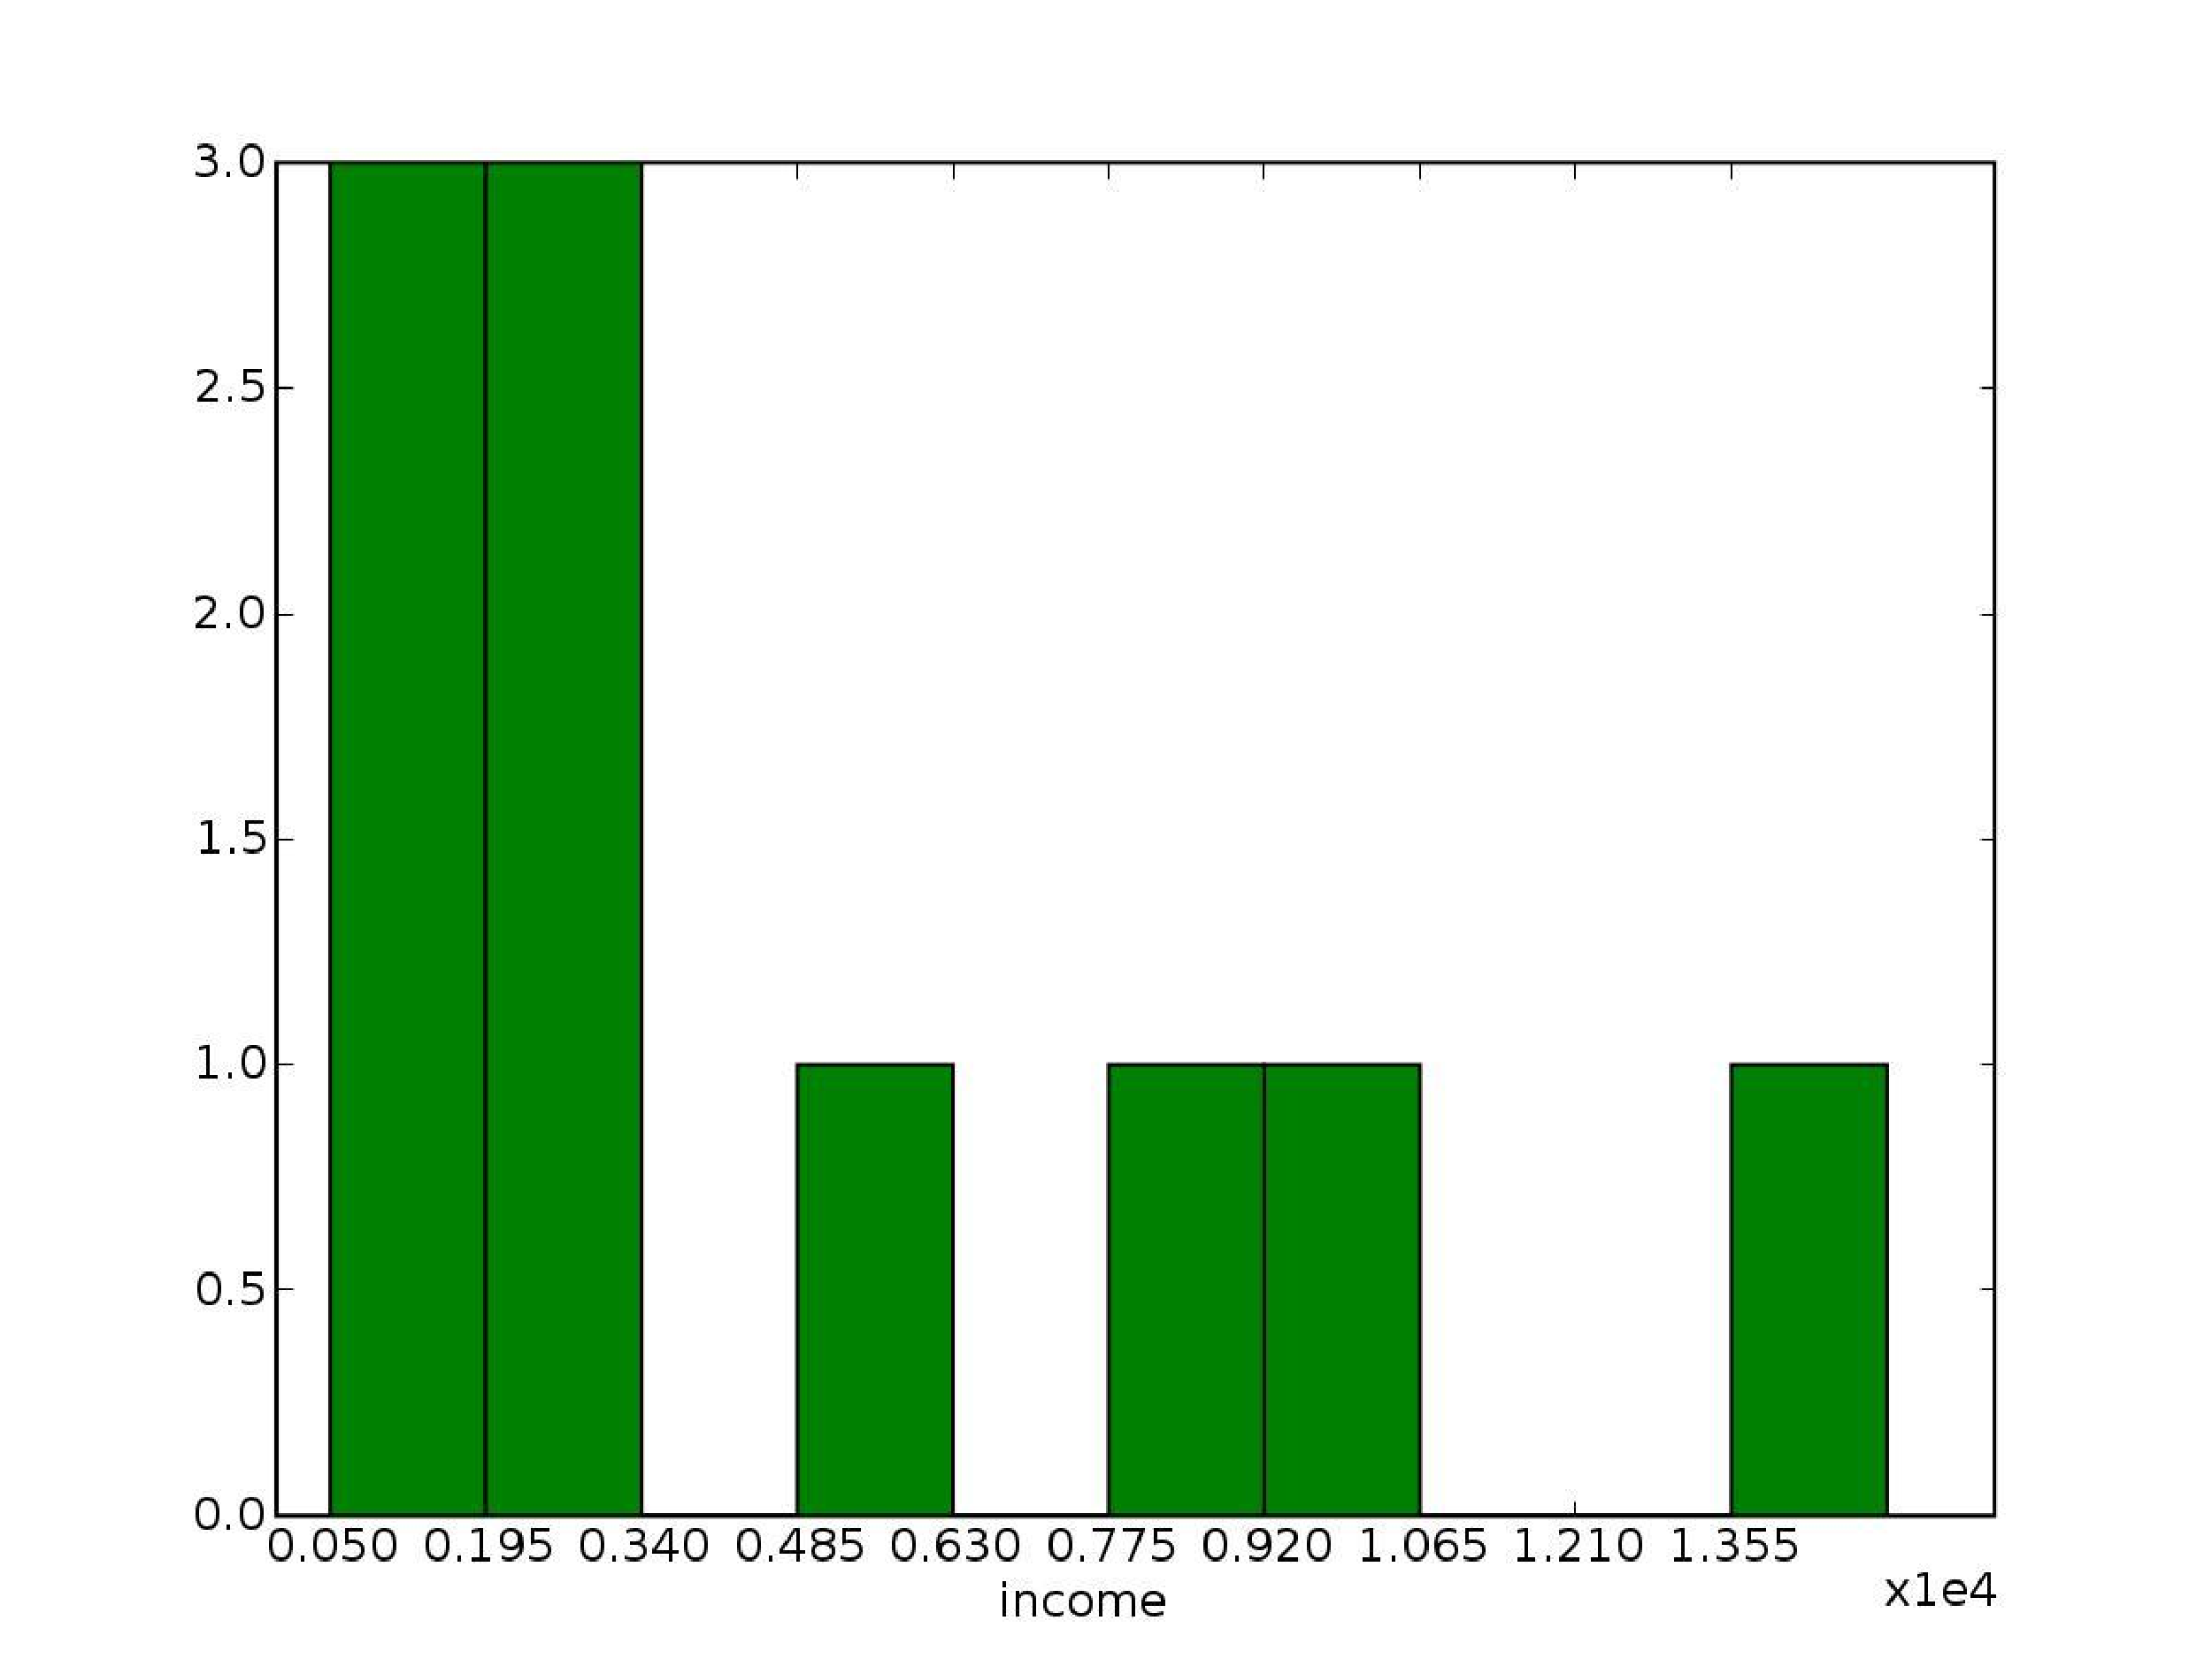
\includegraphics[scale=0.2, angle=0]{images/incomehist.pdf}
%end{latexonly}
\htmlonly{\includegraphics[scale=0.6, angle=0]{images/incomehist.jpg}}
\end{center}
or (if the \module{rpy} \rpyindex library is installed)
\begin{verbatim}
>>> households.r_histogram("income")
\end{verbatim}
\begin{center}
%begin{latexonly}
\includegraphics[scale=0.3, angle=90]{images/incomerhist.pdf}
%end{latexonly}
\htmlonly{\includegraphics[scale=0.3, angle=90]{images/incomerhist.jpg}}
\end{center}

We can investigate a correlation \index{correlation} between attributes \attributesindex by plotting a scatter
plot \scatterplotindex (\module{rpy} \rpyindex library required):

\begin{verbatim}
>>> households.r_scatter("persons", "income")
\end{verbatim}
\begin{center}
%begin{latexonly}
\includegraphics[scale=0.3, angle=90]{images/incomerscatter.pdf}
%end{latexonly}
\htmlonly{\includegraphics[scale=0.3, angle=90]{images/incomerscatter.jpg}}
\end{center}
\coefficientsindex
\begin{verbatim}
Correlation coefficient:  0.919147133827
\end{verbatim}

The correlation coefficient between two attributes and the correlation matrix of several attributes, respectively,
can be obtained by:
\begin{verbatim}
>>> households.correlation_coefficient("persons", "income")
0.91914713382720947
>>> households.correlation_matrix(["persons", "income"])
array([[ 1.        ,  0.91914713],
       [ 0.91914713,  1.        ]], type=float32)
\end{verbatim}

A summary of data in a dataset \datasetindex can by given by:

\attributesindex
\begin{verbatim}
>>> households.summary()
Attribute name        mean           sd           sum        min     max
-------------------------------------------------------------------------
       persons         2.7         1.34            27          1       5
        income      4850.0      4749.56         48500        500   15000
       


Size: 10  records
identifiers:
        household_id  in range  1 - 10
\end{verbatim}

To add an attribute \attributesindex to the set of households, for example each
household's location, we do
\begin{verbatim}
>>> households.add_primary_attribute(data=[4,6,9,2,4,8,2,1,3,2], name="location")
>>> households.get_attribute_names()
['household_id', 'persons', 'location', 'income']
\end{verbatim}
If the attribute \attributesindex "location" already exists in the dataset, \datasetindex the values are
overwritten.

To change specific values in a dataset, \datasetindex one can use

\attributesindex
\begin{verbatim}
>>> households.modify_attribute(name="location", data=[0,0], index=[0,1])
>>> households.get_attribute("location")
array([0, 0, 9, 2, 4, 8, 2, 1, 3, 2])
\end{verbatim}
Here the argument \verb|index| determines the index of the data that are
modified.

To determine the location of household with \verb|household_id| $= 5$,
do
\begin{verbatim}
>>> households.get_data_element_by_id(5).location
4
\end{verbatim}

In order to store data in one of the supported formats,
you can use the {\tt storage} object created at the beginning of this section, or create a new one using
a different type of storage:

\datasetindex
\begin{verbatim}
>>> households.write_dataset(out_storage=storage,
                             out_table_name="households_output")
\end{verbatim}

Each dataset \datasetindex
  should have a unique dataset \datasetindex name that is used as an identification in
  variable \variablesindex computation (see
  Section~\ref{sec:variable-names}). 

\begin{verbatim}
>>> households.get_dataset_name()
'household'
\end{verbatim}

The \package{urbansim} package contains many pre-defined dataset \datasetindex classes, such as \class{HouseholdDataset}, \class{GridcellDataset},
  \class{JobDataset}, \class{ZoneDataset}, \class{FazDataset}, \class{NeighborhoodDataset}, \class{RaceDataset},
  \class{RateDataset}. Some datasets are described in  Section~\ref{sec:urbansim-datasets},
  Table~\ref{tab:urbansim-datasets}. They are all children of \class{Dataset} with pre-defined values
  for some arguments, such as \verb|id_name|, \verb|in_table_name| or \verb|dataset_name|. 

  

%
\section{Working with Models}
%
Generally, each model class has a method \method{run()} that runs a simulation and
(if applicable) a method \method{estimate()} that runs an estimation of the model.
Models are initiated by a constructor that sets class attributes common to
both methods.

%
\subsection{Choice Model}
%
The class \class{ChoiceModel} implemented in \package{opus_core} is initiated with a choice set
and a set of components specifying some of the model behavior. The model can
be estimated and run for a set of agents (see Section~\ref{sec:choice-model} for details).

%
\subsubsection{Initialization}
%
Suppose we would like to simulate a process of households deciding among 3
choices using the discrete choice model theory. The number of persons in each
household should influence their decisions. We will model this behavior by
multinomial logit using a system of utility functions:
$$
\begin{array}{rcrr}
v_1 & = &\beta_{01} & \\
v_2 & = &  & \beta_{12}x \\
v_3 & = & \beta_{03} & +  \beta_{13}x
\end{array}
$$
Here, $\beta_{01}$ and $\beta_{03}$ are alternative specific constants and $x$
is a household variable \variablesindex ``persons''.

The model is initialized by
\begin{verbatim}
>>> from opus_core.choice_model import ChoiceModel
>>> choicemodel = ChoiceModel(
                       choice_set=[1,2,3],
                       utilities = "opus_core.linear_utilities",
                       probabilities = "opus_core.mnl_probabilities",
                       choices = "opus_core.random_choices")
\end{verbatim}
Thus, the model is composed by external implementations of model steps, such
as computing utilities, computing probabilities and computing choices,
specified as \module{package.module_name}. Those modules must contain a
class of the same name and a method \method{run()} that performs the actual
computation (see Section~\ref{sec:choice-model} and Sections~\ref{sec:utilities}-\ref{sec:choices}
for more details).

%
\subsubsection{Estimation}
%
In order to estimate coefficients \coefficientsindex $\beta$ from the above equations, we define
a specification:

\coefficientsindex \variablesindex
\begin{verbatim}
>>> from numpy import array
>>> from opus_core.equation_specification import EquationSpecification
>>> specification = EquationSpecification(
      coefficients = array([
        "beta01",      "beta12",         "beta03",    "beta13"
                          ]),
      variables = array([
        "constant","household.persons", "constant", "household.persons"
                        ]),
      equations = array([
           1,              2,                3,             3
                    ])
      )
\end{verbatim}
Each of the arguments is an array where the $i$th element describes the $i$th
coefficient \coefficientsindex in an equation determined by the $i$th element in the argument
\verb|equations|. For example, \verb|beta12| is a coefficient \coefficientsindex connected to the
household variable \variablesindex ``persons'' in equation 2, and \verb|beta03| is a constant
used in equation 3. The prefix ``household'' in the variable \variablesindex name specifies
the name of the dataset \datasetindex \verb|households|.
In other words, we are using here a dataset-qualified \datasetindex name of an attribute \attributesindex explained in
Section~\ref{sec:opus-core-attribute-names}.
An optional argument \verb|submodels| can extend the specification
to a model with multiple submodels. The \class{EquationSpecification} class is described
in Section~\ref{sec:specification} in more detail.

Our estimation data must include an attribute \attributesindex specifying choices that
households made:
\begin{verbatim}
>>> households.add_primary_attribute(data=[1,2,2,2,1,3,3,1,2,1], name="choice_id")
\end{verbatim}

The estimation is done by passing the specification, the agent set for
estimation and a name of the module that implements the actual estimation to
the method \method{estimate()}:
\coefficientsindex
\begin{verbatim}
>>> coefficients, other_results = choicemodel.estimate(
                         specification, households, 
                         procedure="opus_core.bhhh_mnl_estimation")
\end{verbatim}
\begin{verbatim}
Estimating Choice Model (from opus_core.choice_model): started on 
                                                    Wed Nov  5 12:04:17 2008
    submodel: -2
    Convergence achieved.
    Akaike's Information Criterion (AIC):  26.142396805
    Number of Iterations:  144
    ***********************************************
    Log-likelihood is:            -9.07119840248
    Null Log-likelihood is:       -10.9861228867
    Likelihood ratio index:       0.174303938155
    Adj. likelihood ratio index:  -0.189791752496
    Number of observations:       10
    Suggested |t-value| >         1.51742712939
    Convergence statistic is:     0.000990037670084
    -----------------------------------------------
    Coeff_names	estimate	std err		t-values
        beta01	0.432678	 3.14438	0.137604
        beta03	-4.51824	 21.7087	-0.208131
        beta12	0.180115	 1.72541	 0.10439
        beta13	 1.34052	 4.18176	0.320564
    ***********************************************
    Elapsed time:  0.064521 seconds
Estimating Choice Model (from opus_core.choice_model): completed.........0.1 sec

\end{verbatim}
The estimation module given in the argument \verb|procedure| is a child of
\class{EstimationProcedure} (see Section~\ref{sec:estimation-procedure}), must
contain a method \method{run()} and should return a dictionary with keys
''estimators'' and ``standard_errors'' respectively, that contain arrays of
the estimated values and their standard errors, respectively.  The \method{estimate()}
method returns a tuple where the first element is an instance of
class \class{Coefficients} \coefficientsindex and the second element is a dictionary with all
results returned by the estimation \verb|procedure|.

A coefficient \coefficientsindex object can
be stored in a storage. For example, to store the computed coefficients \coefficientsindex as an
ASCII file \file{mycoef.tab} in the directory defined in the \verb|storage| object
on page~\pageref{storagepage}, do
\coefficientsindex
\begin{verbatim}
>>> coefficients.write(out_storage=storage, out_table_name="mycoef")
\end{verbatim}
Again, other types of storage can be used here.

 %

\subsubsection{Simulation}
%
The coefficients \coefficientsindex that result from the estimation run can be directly plugged
into a simulation run:
\coefficientsindex
\begin{verbatim}
>>> choices = choicemodel.run(specification,  coefficients, households)
Running Choice Model (from opus_core.choice_model): 
                                            started on Wed Nov  5 12:10:20 2008
    Total number of individuals: 10
    ChoiceM chunk 1 out of 1.: started on Wed Nov  5 12:10:20 2008
        Number of agents in this chunk: 10
    ChoiceM chunk 1 out of 1.: completed.................................0.0 sec
Running Choice Model (from opus_core.choice_model): completed............0.0 sec
>>> choices
array([1, 2, 1, 2, 2, 3, 3, 1, 2, 3])
\end{verbatim}
The resulting \verb|choices| is an array specifying the choice for each household. We can
now assign those values to the dataset: \datasetindex
\begin{verbatim}
>>> households.modify_attribute(name="choice_id", data=choices)
\end{verbatim}

Note that multiple runs will produce different results, which is due to random
numbers \index{random numbers} used within the model. In order to receive reproducible results\index{reproducible results}, one
can fix the seed of the random number generator. The call above was
preceded by
\numpyindex
\begin{verbatim}
>>> from numpy.random import seed
>>> seed(1)
\end{verbatim}

For demonstration purposes, we use the same dataset of households
for estimation and simulation. This would not be usually the case in real
simulation runs.

We can also create a coefficient \coefficientsindex class and assign their values directly
(see Section~\ref{sec:coefficients} for more details):
\coefficientsindex
\begin{verbatim}
>>> from opus_core.coefficients import Coefficients
>>> coefficients = Coefficients(
                     names=array(["beta01", "beta12", "beta03", "beta13"]),
                     values=array([0.5,      0.2,       -5.0,     1.3]))
\end{verbatim}

If a variable \variablesindex $x$ in the utility equations is choice dependent,
one can create a dataset \datasetindex of choices and assign this attribute to the
dataset. \datasetindex Besides a list and an array, the argument \verb|choice_set| in the
\class{ChoiceModel} constructor also accepts a dataset. \datasetindex

%
\subsection{Location Choice Model}
%
\label{sec:LCM}
%
The \class{LocationChoiceModel} class implemented in \package{urbansim} is a special case of the
\class{ChoiceModel} class (see Section~\ref{sec:location-choice-model} for details).
The choice set is a set of locations that agents choose
from. A set of locations can be sampled to each agent.

Suppose that in addition to the set of 10 households, we have a set of 9
locations with the attributes cost of living and capacity, respectively,
stored in a file \file{locations.tab}:
\begin{verbatim}
location  cost  capacity
1        500    1
2        200    1
3        600    2
4       1000    3
5        100    1
6       2000    3
7        300    1
8        400    1
9        800    2
\end{verbatim}
One can represent this dataset using again the  \class{Dataset} class:
\label{page:tutorial-gc-locations}
\begin{verbatim}
>>> locations = Dataset(in_storage = storage,
                        in_table_name = 'locations', 
                        id_name='location',
                        dataset_name='gridcell')
\end{verbatim}
We use here the \verb|storage| object
created on page~\pageref{storagepage}, since the table is stored in the same directory.

Suppose, we wish to simulate a process of agents choosing locations.  As a
first example, suppose our only predictor is the location attribute cost with
a coefficient \coefficientsindex value of $-0.01$ (modeling a negative effect of cost on the
choice preferences). (For simplicity, we skip the estimation process and
consider the coefficient \coefficientsindex value as given.) As in the previous section, we
create a coefficient \coefficientsindex object, a specification object and a choice model object,
respectively:

\coefficientsindex \variablesindex
\begin{verbatim}
>>> coefficients = Coefficients(names=("costcoef", ), values=(-0.01,))
>>> specification = EquationSpecification(variables=("gridcell.cost", ),
                                          coefficients=("costcoef", ))
>>> from urbansim.models.household_location_choice_model import \
                               HouseholdLocationChoiceModel
>>> hlcm = HouseholdLocationChoiceModel(
                               location_set = locations,
                               sampler=None,
                               compute_capacity_flag=False)
\end{verbatim}
The household location choice model (HLCM) is a child of 
\class{LocationChoiceModel} with some useful default settings.  
The argument \verb|sampler| specifies a module to be
used for sampling locations to each agent. If it is None, all locations are
considered as a possible alternative for each agent.  The argument
\verb|compute_capacity_flag| specifies if the procedure should take capacity of
locations into account.

We can run the HLCM by using the method \method{run()}
which takes as obligatory arguments \verb|specification|, \verb|coefficients| \coefficientsindex
and the set of agents for which the model runs.  
\coefficientsindex
\begin{verbatim}
>>> seed(1)
>>> result = hlcm.run(specification, coefficients, agent_set=households)
Running Household Location Choice Model 
                 (from urbansim.models.household_location_choice_model): 
                                     started on Wed Nov  5 12:53:11 2008
    Total number of individuals: 10
    HLCM chunk 1 out of 1.: started on Wed Nov  5 12:53:11 2008
        Number of agents in this chunk: 10
    HLCM chunk 1 out of 1.: completed....................................0.0 sec
Running Household Location Choice Model 
      (from urbansim.models.household_location_choice_model): completed...0.0 sec

\end{verbatim}

The results of the HLCM run determine locations that
agents have chosen. The model modifies values of the attribute \attributesindex `location' of
the agent set or adds this attribute \attributesindex to the dataset, \datasetindex if it doesn't exist:
\attributesindex
\begin{verbatim}
>>> households.get_attribute("location")
array([5, 5, 5, 5, 5, 7, 7, 2, 5, 5])
\end{verbatim}

One way of visualizing results of the HLCM run is to plot a histogram \histogramindex of the
choices, including the capacity of each location (requires \module{matplotlib}
library):

\begin{verbatim}
>>> hlcm.plot_choice_histograms(capacity=locations.get_attribute("capacity"))
\end{verbatim}
\begin{center}
%begin{latexonly}
\includegraphics[scale=0.5, angle=0]{images/hlcmhist.pdf}
%end{latexonly}
\htmlonly{\includegraphics[scale=0.6, angle=0]{images/hlcmhist.jpg}}
\end{center}
In our case, more agents decided for the fifth and seventh location than there
are units available (which corresponds to the fact that those are two of the three cheapest locations).

In the above example, the discrete choice model consists of steps such as
computing utilities via the \class{opus_core.linear_utilities} class, computing
probabilities via the \class{opus_core.mnl_probabilities} class and computing
choices via the \class{opus_core.random_choices} class. These components
(default values) can be easily exchanged by other implementations. For
example, the class \class{urbansim.lottery_choices} for computing choices
takes into account capacity and forces agents to re-decide, if there is an
overflow in the locations capacity:
\begin{verbatim}
>>> number_of_agents = "gridcell.number_of_agents(household)"
>>> hlcm2 = HouseholdLocationChoiceModel(
                         location_set = locations,
                         sampler=None,
                         choices="urbansim.lottery_choices",
                         compute_capacity_flag=True,
                         capacity_string="capacity",
                         number_of_agents_string=number_of_agents,
                         number_of_units_string="capacity",
                         run_config={"lottery_max_iterations":10})
\end{verbatim}

The argument \verb|choices| is the full name of the module in which the choice
class is implemented. This module
must contain a class of the same name, i.e.
\class{lottery_choices} in this case, be a child of \package{opus_core} class \class{Choices}
(see Section~\ref{sec:choices}) and have a method \method{run()}.  Further arguments define the name of
the capacity attribute, \attributesindex name of the variable \variablesindex that computes number of agents in
each location (more about variable \variablesindex names in Section~\ref{sec:variable-names}), name of the
variable/attribute \attributesindex \variablesindex that determines the total number of units for each location. 
The argument \verb|run_config| is a dictionary that contains parameters for the simulation. In this example it contains a value
of how many times the households can re-decide if there is an overflow.

We run the above model:
\begin{verbatim}
>>> seed(1)
>>> result = hlcm2.run(specification, coefficients, households)
Running Household Location Choice Model 
                     (from urbansim.models.household_location_choice_model): 
                                            started on Wed Nov  5 18:18:58 2008
    Total number of individuals: 10
    HLCM chunk 1 out of 1.: started on Wed Nov  5 18:18:58 2008
        Number of agents in this chunk: 10
        Available capacity: 15.0 units.
        Number of unplaced agents: 0 (in 4 iterations)
    HLCM chunk 1 out of 1.: completed....................................0.0 sec
    gridcell.number_of_agents(household).................................0.0 sec
Running Household Location Choice Model 
     (from urbansim.models.household_location_choice_model): completed...0.0 sec
>>> hlcm2.plot_choice_histograms(capacity=locations.get_attribute("capacity"))
\end{verbatim}
\begin{center}
%begin{latexonly}
\includegraphics[scale=0.5, angle=0]{images/hlcm2hist.pdf}
%end{latexonly}
\htmlonly{\includegraphics[scale=0.6, angle=0]{images/hlcm2hist.jpg}}
\end{center}
\attributesindex
\begin{verbatim}
>>> households.get_attribute("location")
array([9, 3, 9, 5, 4, 3, 7, 2, 8, 1])
\end{verbatim}
Now there is no overflow. Moreover, fourth and sixth locations still have free
units available, since they are the most expensive places. The agents were `forced'
to re-decide three times (i.e. 4 iterations in total). If the maximum
number of iterations given in \verb|run_config| would be reached without
placing all agents, the whole model would run automatically again. It would not be
very useful in this simple example, but the model is set-up for more complex situations,
including sampling of locations. Therefore in a new run, agents would sample
different locations which could solve the collision from the previous run.

Finally, agents that were not
placed have values smaller equal zero in the ``location'' attribute. \attributesindex

\package{urbansim} implements several location choice models.
Figure~\ref{fig:urbansim-model} in Section~\ref{sec:urbansim-models} shows
a hierarchical structure of the models.


%
\subsection{Regression Model}
%
\label{sec:RM}
%
Opus offers an infrastructure for estimation and simulation of a regression model
(see Section~\ref{sec:regression-model} for details).
Suppose our set of grid cells from the previous section has an attribute
``distance_to_cbd'' that contains information about the distance to the
central business district (cbd):

\begin{verbatim}
location cost  distance_to_cbd
1        500             5
2        200            10
3        600             5
4       1000             1
5        100            20
6       2000             0
7        300             7
8        400             7
9        800             3
\end{verbatim}

One can add the new attribute to the existing set of locations by:
\begin{verbatim}
>>> locations.add_primary_attribute(name="distance_to_cbd",
                                    data=[5,10,5,1,20,0,7,7,3])
\end{verbatim}

The cost of living in this dataset is highly correlated with
the distance to cbd and we can thus predict the cost using the regression model.

%
\subsubsection{Initialization}
%
The model is initialized by:
\begin{verbatim}
>>> from opus_core.regression_model import RegressionModel
>>> rm = RegressionModel(regression_procedure="opus_core.linear_regression")
\end{verbatim}
As in the case of choice model, the model is composed by model components, here
by plugging the appropriate regression procedure. The
regression procedure is a child of \class{Regression} (see Section~\ref{sec:regression}),
must have a method \method{run()} that gets as arguments a
multidimensional data array and a one-dimensional array of coefficients, \coefficientsindex and
returns a one-dimensional array of the regression outcome.

The \class{linear_regression} module implemented in \package{opus_core} is the default
procedure for the \class{RegressionModel} constructor and thus, it can be omitted.

%
\subsubsection{Estimation}
%
The specification for the above example consists of one variable \variablesindex and one
constant for the intercept:
\variablesindex
\begin{verbatim}
>>> specification = EquationSpecification(
                          variables=array(["constant", "gridcell.distance_to_cbd"]),
                          coefficients=array(["constant", "dcbd_coef"]))
\end{verbatim}
The estimation for predicting the cost of living is run by:
\begin{verbatim}
>> coef, other_results = rm.estimate(specification, dataset=locations,
                              outcome_attribute="gridcell.cost",
                              procedure="opus_core.estimate_linear_regression")
Estimating Regression Model (from opus_core.regression_model):
                                            started on Mon Mar 19 21:14:33 2007
    Estimate regression for submodel -2
    Number of observations: 9
    R-Squared:             0.536420010196
    Adjusted R-Squared:    0.470194297367
    Suggested |t-value| >  1.48230380737
    -----------------------------------------------
    Coeff_names estimate        SE      t-values
      constant   1114.07         213.758         5.21183
     dcbd_coef  -71.1493         24.9995        -2.84603
    ===============================================

Estimating Regression Model (from opus_core.regression_model): completed...0.4 sec
\end{verbatim}
The estimation procedure that is passed as an argument is expected to be
a child of \class{EstimationProcedure} (see Section~\ref{sec:estimation-procedure}) and have a
method \method{run()} that takes as arguments a
multidimensional data array and an instance of a class specified by the
argument \verb|regression_procedure| in the model constructor. Thus, the
estimation procedure can use the same code that is used for simulation.

The resulting object of class \class{Coefficients} \coefficientsindex called \verb|coef| can be stored or
directly used for predicting cost of other locations.
\coefficientsindex
\begin{verbatim}
>>> coef.summary()
Coefficient object:
size: 2
names: ['constant' 'dcbd_coef']
values:
[ 1114.07348633   -71.14933777]
standard errors:
[ 213.75848389   24.99952126]
t_statistic:
[ 5.211833   -2.84602809]
submodels: [-2 -2]
\end{verbatim}

%
\subsubsection{Simulation}
%
Suppose we have four locations with distance to cbd 2, 4, 6 and 8
respectively. We create a location dataset \datasetindex using
a storage type `dict'\index{Storage!dict}.
This type of storage is useful when we want to pass data directly without storing them on a physical storage media.

\begin{verbatim}
>>> dstorage = StorageFactory().get_storage('dict_storage')
>>> dstorage.write_table(table_name='gridcells',
                         table_data= {'id':array([1,2,3,4]),
                                      'distance_to_cbd':array([2,4,6,8])
                                    })
>>> ds = Dataset(in_storage=dstorage, in_table_name='gridcells',
                 id_name='id', dataset_name='gridcell')
\end{verbatim}
We have created a table in the RAM space called \file{gridcells} which is passed into the \class{Dataset} constructor.
Now we run the regression model with coefficients \coefficientsindex estimated in the previous
section:
\coefficientsindex \datasetindex
\begin{verbatim}
>>> cost = rm.run(specification, coefficients=coef, dataset=ds)
Running Regression Model (from opus_core.regression_model):
                                        started on Mon Mar 19 21:35:23 2007
    Total number of individuals: 4
    RM chunk 1 out of 1.: started on Mon Mar 19 21:35:23 2007
        Number of agents in this chunk: 4
    RM chunk 1 out of 1.: completed......................................0.0 sec
Running Regression Model (from opus_core.regression_model): completed....0.0 sec
>>> cost
array([ 971.77478027,  829.47613525,  687.17749023,  544.87878418])
\end{verbatim}
As expected, the resulting cost decreases with increasing distance to cbd.

%
\section{Opus Variables} \index{Variables!Opus}
%
\label{sec:variables}
%
\subsection{Variable Concept}
%
\label{sec:variableconcept}
%
\variablesindex

As mentioned in Section~\ref{sec:datasets}, a dataset \datasetindex has a set of
attributes, \attributesindex such as income or persons, that are stored in a file or database.
We call such characteristics {\it primary attributes}. \primaryattributesindex In addition, one is usually
interested in attributes \attributesindex that are computed, for example using some
transformation of primary attributes. \primaryattributesindex We call those attributes \attributesindex {\it
variables}, \variablesindex or {\it computed attributes}. \computedattributesindex They are simply handled as additional
``columns'' of a dataset \datasetindex to which they belong to, here denoted as
``parent dataset''. \datasetindex

In Opus, a variable \variablesindex is a class derived from the
\package{opus_core} class \class{Variable}\variablesindex.  Opus expressions 
(Chapter~\ref{chapter:expressions}),
as used in the expression library in the GUI and elsewhere, in fact just
are compiled into an automatically generated subclass of class \class{Variable}.
Section~\ref{sec:opus-variable} gives additional details about this class, 
including a discussion of how expressions are compiled.

In the GUI description, we used the expression library as a place to store and
reuse variable definitions.  We can also write expressions as Python strings
and use them from the command line.  The syntax of these expression language is 
that of Python, but the semantics
are somewhat different --- for example, a name like
\code{gridcell.distance_to_cbd} is a reference to the value of that
variable.  (If you just evaluated this in a Python shell you'd get an
error, saying that the \package{gridcell} package didn't have a
\code{distance_to_cbd} attribute.)  Further, expressions are evaluated lazily.
Here is a simple example:

\begin{verbatim}
>>> locations.compute_variables(["sqrt(gridcell.distance_to_cbd)"])
array([ 2.23606798,  3.16227766,  2.23606798,  1.        ,  4.47213595,
        0.        ,  2.64575131,  2.64575131,  1.73205081])
\end{verbatim}

The expressions are fed to the \method{compute_variables} method 
\index{compute_variables} of
\class{Dataset} (Section \ref{sec:compute-variables}), just as for simple
variable references.  (Given a new expression, Opus will compose a
new variable definition, including a \method{compute} and a
\method{dependencies} method, which computes the value of that expression.
It then saves the new variable definition in case the same expression is
encountered again --- see Section~\ref{sec:implementation-of-expressions}.
However, usually the user need not
be concerned about this.)  The \method{compute_variables} method evaluates
each variable (or expression) in turn, and returns the value of the last one.

For variables defined by hand as Python classes (rather than using Tekoa expressions), the
name of the class for a given variable is identical to the name of the module 
in which it is implemented.
The module is stored in a directory whose name corresponds to the name of
the parent dataset. \datasetindex Note that the variable \variablesindex 
name must be all lower case.

The variable \variablesindex class must have a method \method{compute()} 
that returns a numpy array of
variable \variablesindex values. The size of that array must correspond to the number of entries in the parent
dataset. \datasetindex The \method{compute()} method takes an argument called
\verb|dataset_pool| containing references to the appropriate set of datasets to
use for computing this variable. From the \method{compute()} method, the parent dataset \datasetindex can be
accessed  by \method{self.get_dataset()}.

If the variable depends on other attributes, they must be listed in the method
\method{dependencies()}, which returns a list of all dependent variables and
attributes in their fully-qualified names (see
Section~\ref{sec:opus-core-attribute-names} for details on attribute
specification).

As an example, consider a variable ``is_in_wetland'' for the gridcell dataset
\verb|locations| from Sections~\ref{sec:LCM} and~\ref{sec:RM}. The variable
returns \verb|True| for entries whose percentage of wetland is more than a certain
threshold, and \verb|False| otherwise. The module \file{is_in_wetland.py},
containing a class \class{is_in_wetland}, is stored in the directory
\file{gridcell} because
\begin{verbatim}
>>> locations.get_dataset_name()
'gridcell'
\end{verbatim}

The class is defined as follows:
\variablesindex
\begin{verbatim}
from opus_core.variables.variable import Variable
class is_in_wetland(Variable):

    def dependencies(self):
        return ["gridcell.percent_wetland"]

    def compute(self, dataset_pool):
        return self.get_dataset().get_attribute("percent_wetland") > \
         dataset_pool.get_dataset('urbansim_constant')["percent_coverage_threshold"]

\end{verbatim}
The dependent attribute is a primary attribute and therefore specified as
a dataset-qualified name.  For our example, we populate the primary attribute:
\begin{verbatim}
>>> locations.add_primary_attribute(name="percent_wetland",
                                    data=[85,20,0,90,35,51,0,10,5])
\end{verbatim}

\begin{figure}[th]
\begin{verbatim}
from opus_core.variables.variable import Variable
from urbansim.functions import attribute_label
from variable_functions import my_attribute_label
from opus_core.logger import logger

class population(Variable):
    """Compute the total number of people residing in a gridcell, 
    by summing hh_persons over all households in the gridcell"""
    
    _return_type="int32"
    hh_persons = "persons"

    def dependencies(self):
        return [attribute_label("household", self.hh_persons), 
                attribute_label("household", "grid_id"), 
                my_attribute_label("grid_id")]

    def compute(self, dataset_pool):
        households = dataset_pool.get_dataset('household')
        return self.get_dataset().sum_dataset_over_ids(households, self.hh_persons)


from opus_core.tests import opus_unittest
from opus_core.tests.utils.variable_tester import VariableTester
from numpy import array
class Tests(opus_unittest.OpusTestCase):
    def test_my_inputs(self):
        gridcell_grid_id = array([1, 2, 3])
        #specify an array of 4 hh's, 1st hh's grid_id = 2 (it's in gridcell 2), etc.
        household_grid_id = array([2, 1, 3, 2]) 
        #specify how many people live in each household
        hh_persons = array([10, 5, 20, 30])

        tester = VariableTester(
            __file__,
            package_order=['urbansim'],
            test_data={
                "gridcell":{
                    "grid_id":gridcell_grid_id 
                    }, 
                "household":{ 
                    "household_id":array([1,2,3,4]),
                    "persons":hh_persons, 
                    "grid_id":household_grid_id
                }
            }
        )
        
        should_be = array([5, 40, 20])
        tester.test_is_close_for_family_variable(self, should_be)

if __name__=='__main__':
    opus_unittest.main()
\end{verbatim}
\caption{Definition of the `population' variable as a Python class}
\label{fig:population-variable}
\end{figure}

As another example, consider the \code{population} variable to compute
the population in each gridcell.  We refer
to a variable using a \verb#Pythonpath#, which provides a means for
Python to find modules and classes in a directory structure.  So, a
reference to this particular module using a \emph{fully qualified path}
would be \code{urbansim.gridcell.population}.  You can find all of the
existing variables by browsing on disk in the source code directory. 
The directory structure mirrors the parts of the variable name, so that
\code{urbansim.gridcell.population} is really pointing to
\file{opus/src/urbansim/gridcell/population.py}, which is also included 
in Figure~\ref{fig:population-variable} on page~\pageref{fig:population-variable}.

\subsubsection{Dataset Pool}
\index{dataset pool}
%
When computing variable values, Opus may need to access datasets used by
dependent variables, such as the \verb|urbansim_constant| dataset required by
\verb|is_in_wetland|, above.  These datasets are provided by the
\verb|dataset_pool| object passed into the variable's \method{compute} method.
This object is an instance of the \class{DatasetPool} class (see Section~\ref{sec:core-dataset-pool}).  It is responsible
for keeping a set of datasets for use when computing
variables.  If the requested dataset is in the pool already, it is returned
directly, otherwise it tries to find it in the given storage.

In order to find the appropriate dataset class for the requested dataset, the dataset
pool object searches the \file{datasets} directories of the Opus packages in
\verb|package_order|.  The first one to contain the appropriately named module
and class is used.  For instance, using the \verb|storage| object created on page~\pageref{storagepage},
for the definition:
\begin{verbatim}
>>> from opus_core.dataset_pool import DatasetPool
>>> dataset_pool = DatasetPool(package_order=['urbansim', 'opus_core'],
                               storage=storage)
\end{verbatim}
if \verb|dataset_pool| is asked for the ``household'' dataset, and does not
already have one in its pool, it will look in the \verb|storage|. In order to
create the corresponding dataset classes
it searches for a file
\file{household_dataset.py} (containing the class \class{HouseholdDataset}) first in \file{urbansim/datasets} and then in
\file{opus_core/datasets}. The first one found will be used.
\begin{verbatim}
>>> dataset_pool.datasets_in_pool()
{}
>>> hs = dataset_pool.get_dataset("household")
>>> dataset_pool.datasets_in_pool()
{'household': <urbansim.datasets.household_dataset.HouseholdDataset object
                                                               at 0x197c2f70>}
>>> hs.size()
10
\end{verbatim}
If the dataset pool is asked for \verb|urbansim_constant| and `urbansim' is included in \verb|package_order|,
it will use some \package{urbansim} specific constants defined in \file{urbansim/constants.py} (in addition to
user defined constants found on storage).

For the purpose of this example, we set the required constant by:
\begin{verbatim}
>>> constant = dataset_pool.get_dataset("urbansim_constant")
>>> constant["percent_coverage_threshold"] = 50
\end{verbatim}

\subsubsection{Invoking Computation}
\label{sec:compute-variables}
Computation of a variable is invoked using the \class{Dataset} method
\method{compute_variables()} passing the variable name in its fully-qualified
form and a dataset pool if other datasets are required for this variable:
 \label{page:compute-isnearcbd}
\variablesindex
\begin{verbatim}
>>> locations.compute_variables("urbansim.gridcell.is_in_wetland",
                                  dataset_pool=dataset_pool)
urbansim.gridcell.is_in_wetland..........................................0.0 sec
array([ True, False, False,  True, False,  True, False, False, False], dtype=bool)
\end{verbatim}

The method returns the resulting values of the variable. The
\verb|compute_variables| method also accepts a list of variables to be
computed.  In this case it returns values of the last variable in the list.

 In addition, within the dataset, the variable can be accessed using its un-qualified name.
 Thus, the un-qualified names of variables including the primary
 attributes must be unique.
\begin{verbatim}
>>> locations.get_attribute("is_in_wetland")
array([ True, False, False,  True, False,  True, False, False, False], dtype=bool)
\end{verbatim}

\subsection{Interaction Variables}
\label{sec:interactions}

In order to work with variables \variablesindex that determine an
interaction between two datasets, \datasetindex there is a subclass of
\class{Dataset}, called
\class{InteractionDataset}. Attributes of this class are stored as
two-dimensional arrays (see Section~\ref{sec:interaction-set} for details).

To create an interaction set for households and gridcells from the previous
sections, do
\begin{verbatim}
>>> from opus_core.datasets.interaction_dataset import InteractionDataset
>>> interactions = InteractionDataset(dataset1 = households, dataset2 = locations)
\end{verbatim}
The dataset name is composed from dataset names of the two interacting datasets: \datasetindex
\begin{verbatim}
>>> interactions.get_dataset_name()
'household_x_gridcell'
\end{verbatim}
Thus, an interaction variable \variablesindex for such dataset \datasetindex will be implemented in the
directory \file{household_x_gridcell}.

The \class{InteractionDataset} class contains several methods that are useful for
variable \variablesindex computation which must return a two-dimensional array. For example, a
variable \variablesindex defined as a multiplication of cost and income can be implemented as:
\variablesindex
\begin{verbatim}
from opus_core.variables.variable import Variable

class cost_times_income(Variable):
    def dependencies(self):
        return ["gridcell.cost", "household.income"]

    def compute(self, dataset_pool):
        return self.get_dataset().multiply("income", "cost")
\end{verbatim}

This \class{cost_times_income} variable is mostly for illustration; it can
also be defined more conveniently as an expression (see Chapter~\ref{chapter:expressions}).

If we wish that only a subset of each dataset \datasetindex interact (for example for
memory reasons), we can pass the corresponding indices to the constructor:
\index{Memory!Loading a subset of a dataset}
\begin{verbatim}
>>> from numpy import arange
>>> interactions = InteractionDataset(dataset1 = households, dataset2 = locations,
                                  index1 = arange(5), index2 = arange(3))
\end{verbatim}
Here only the first 5 households and the first three gridcells interact.
The \method{compute()} method of the interaction variable \variablesindex should return an array of
size index1 $\times$ index2.

\variablesindex \attributesindex
\begin{verbatim}
>>> interactions.compute_variables(
        ["urbansim.household_x_gridcell.cost_times_income"])
array([[  500000.,   200000.,   600000.],
       [ 1000000.,   400000.,  1200000.],
       [ 2500000.,  1000000.,  3000000.],
       [ 1500000.,   600000.,  1800000.],
       [  250000.,   100000.,   300000.]])
\end{verbatim}
\label{page:compute-interaction}

\package{urbansim} uses interaction variables \variablesindex mainly in \class{ChoiceModel} classes, where agents
interact with dataset \datasetindex of choices. The household location choice model object
\verb|hlcm| from Section~\ref{sec:LCM} can be for example estimated using two
variables, \variablesindex one of which is an interaction variable: \variablesindex
\primaryattributesindex
\begin{verbatim}
>>> specification = EquationSpecification(
                     variables=array([
                          "gridcell.cost",
                          "urbansim.household_x_gridcell.cost_times_income"]),
                     coefficients=array(["costcoef", "cti_coef"]))
>>> # place households
>>> households.add_primary_attribute(data=[2,8,3,1,5,4,9,7,3,6], name="location")
>>> coef, other_results = hlcm.estimate(specification, households)
Estimating Household Location Choice Model 
                     (from urbansim.models.household_location_choice_model): 
                                             started on Thu Nov  6 12:12:47 2008
    urbansim.household_x_gridcell.cost_times_income......................0.0 sec
    submodel: -2
    Convergence achieved.
    Akaike's Information Criterion (AIC):  39.8199022026
    Number of Iterations:  18
    ***********************************************
    Log-likelihood is:            -17.9099511013
    Null Log-likelihood is:       -21.9722457734
    Likelihood ratio index:       0.184882998032
    Adj. likelihood ratio index:  0.0938590753688
    Number of observations:       10
    Suggested |t-value| >         1.51742712939
    Convergence statistic is:     0.000302603242051
    -----------------------------------------------
    Coeff_names estimate        std err         t-values
      costcoef  -0.00312452     0.00339464      -0.920429
      cti_coef  4.45803e-07     5.34429e-07     0.834168
    ***********************************************
    Elapsed time:  0.02 seconds
Estimating Household Location Choice Model 
     (from urbansim.models.household_location_choice_model): completed...0.0 sec
\end{verbatim}
\coefficientsindex
\label{page:iv-spec}

%
\subsection{Versioning}
\label{sec:versioning}
%
Opus uses a mechanism of versioning of variables \variablesindex and attributes. \attributesindex Each
variable/attribute \variablesindex\attributesindex is initialized with a version number 0. Any subsequent
change of that variable/attribute \variablesindex\attributesindex increments the version number. This allow us
to only recompute variables, \variablesindex if it is really needed. This means that if a
computation is invoked (by e.g.\ \verb|compute_variables()|), \variablesindex it is checked, if
any of the version numbers of all dependent variables \variablesindex has changed since the
last computation. The computation is performed only, if there was any change
in the dependencies tree. The mechanism is described in Section~\ref{sec:dependencies-tree}
in more detail.

For example,
\variablesindex
\begin{verbatim}
>>> households.get_version("income")
0
>>> res = interactions.compute_variables([
             "urbansim.household_x_gridcell.cost_times_income"])
>>> interactions.get_version("cost_times_income")
0
>>> households.modify_attribute(name="income", data=[14000], index=[9])
>>> households.get_version("income")
1
>>> res = interactions.compute_variables([
             "urbansim.household_x_gridcell.cost_times_income"])
urbansim.household_x_gridcell.cost_times_income.......................0.0 sec
>>> interactions.get_version("cost_times_income")
1
\end{verbatim}

The first call of \method{compute_variables()} didn't perform the actual
computation, because nothing has changed since our previous computation on
page~\pageref{page:compute-interaction}.
After we modify one element of the ``income'' attribute
(note that ``income'' is a dependent variable of
``cost_times_income'' defined in the \method{dependencies()} method), the
variable is recomputed and the version number is increased.

\subsection{Using Arguments in Variable Names}
\label{sec:tutorial-numbersinvariables}

Opus offers the possibility of including a number or a character string into
variable name which is then passed to the variable constructor as an argument.
The module/class name of such variable corresponds to a pattern in which a
number is replaced by `DDD' and a string is replaced by `SSS'\@.  For example,
a similar variable to \class{is_in_wetland} in Section~\ref{sec:variableconcept} can be
implemented in a way that the threshold is directly included in the variable
name, such as \\
\class{is_in_wetland_if_threshold_is_80}. Here, we give an example of variable
of the type \verb|is_near_|{\em location}\verb|_if_threshold_is_|{\em number}.
As {\em location} we can use e.g. `highway',  `arterial', or `cbd'.
The class name is \class{is_near_SSS_if_threshold_is_DDD} and must have a
constructor implemented which takes a string and a number as arguments:

\variablesindex
\numpyindex
\begin{verbatim}
from opus_core.variables.variable import Variable

class is_near_SSS_if_threshold_is_DDD(Variable):
    def __init__(self, location, number):
        self.location = location
        self.number = number
        Variable.__init__(self)

    def dependencies(self):
        return ["gridcell.distance_to_" + self.location]

    def compute(self, dataset_pool):
        distance_to_location = self.get_dataset().get_attribute(
                                        "distance_to_" + self.location)
        return distance_to_location < self.number
\end{verbatim}
We can then invoke the computation for the `cbd' location and different
thresholds by changing the variable name:
\begin{verbatim}
>>> res = locations.compute_variables(
      map(lambda threshold:
       "urbansim.gridcell.is_near_cbd_if_threshold_is_%s" % threshold, [2,4,7]))
urbansim.gridcell.is_near_SSS_if_threshold_is_DDD...................0.0 sec
urbansim.gridcell.is_near_SSS_if_threshold_is_DDD...................0.0 sec
urbansim.gridcell.is_near_SSS_if_threshold_is_DDD...................0.0 sec
\end{verbatim}

\attributesindex
\begin{verbatim}
>>> locations.get_attribute("is_near_cbd_if_threshold_is_2")
array([False, False, False,  True, False,  True, False, False, False], dtype=bool)
>>> locations.get_attribute("is_near_cbd_if_threshold_is_4")
array([False, False, False,  True, False,  True, False, False,  True], dtype=bool)
>>> locations.get_attribute("is_near_cbd_if_threshold_is_7")
array([ True, False,  True,  True, False,  True, False, False,  True], dtype=bool)
\end{verbatim}

If the dataset \datasetindex \verb|locations| would have an attribute \attributesindex
``distance_to_highway'', we
could use the same variable \variablesindex implementation for variables \variablesindex
\class{is_near_highway_if_threshold_is_...}.

The arguments of the constructor are passed in the same number and order as
they appear in the variable name. For example, if the name would contain only
one pattern, say DDD, the constructor would expect only one argument, namely
an integer. The method \method{dependencies()} is called from
\method{Variable.__init__()}, therefore any class attributes used in
\method{dependencies()} (such as \verb|self.location| in this case) must be set
before the call of \\
\method{Variable.__init__()}.

\emph{Note: Arguments for variable names will probably be replaced with a
  more standard syntax in the future, for example
  \class{is_near(feature='highway', threshhold=2)}.  However, we don't have
  a specific date yet for this change.  We will try to preserve backward
  compatibility.}

\subsection{Expression Names and Aliasing}
\label{sec:urbansim-tutorial-aliasing}
\index{aliasing}

The expression library includes a name field for each expression.  This is
used to bind the name to the corresponding expression.  When using such
expressions intermixed with Python code, another mechanism is needed to
give a name to an expression -- this is done with something much like an
assignment statement, for example:

\code{lnpop = ln(urbansim.gridcell.population)}

This is treated as an expression, which can occur in the list of
expressions given to \method{compute_variables} or in an \file{aliases.py}
file (see below).  The value of the new alias is returned as the value of
the expression if it's the last item on the list of variables and
expressions.

It is convenient, and often more efficient
(Section~\ref{sec:expression-equality}), to gather all the expressions and
aliases for a particular package and dataset into one place.  When using 
XML-based configurations, the expression library component of the XML configurations
supports this nicely.  In older parts of the code using dictionary-based
configurations, the optional
\file{aliases.py}\index{alias.py file} file supports this functionality instead.
This file should define a single variable \code{aliases} to be a list of expressions,
each of which should define an alias.  This file is then placed in the same
directory as variables for that package and dataset.  For example, to
define aliases relevant to \code{urbansim.gridcell}, put an
\file{aliases.py} file into the \file{urbansim.gridcell} directory.  These
aliases can then be referred to using the fully-qualified name of the
alias.  When finding a variable referenced by a fully-qualified name, the
system first searches the aliases file (if present), and then the variable
definitions in the appropriate directory.

As an example, the directory \code{opus_core.test_agent} contains one
variable definition, for the variable \code{income_times_2}.  (This
directory and variable are used for unit tests for \package{opus_core}.)
The file \file{aliases.py} in that same directory contains the following:

\begin{verbatim}
aliases = [
    'income_times_5 = 5*opus_core.test_agent.income',
    'income_times_10 = 5*opus_core.test_agent.income_times_2'
    ]
\end{verbatim}

The first alias refers to a primary attribute (\code{test_agent.income}),
and the second to the variable.  These aliases can then be referred to
using a fully-qualified name, in exactly the same way as a variable,
for example

\code{opus_core.test_agent.income_times_5}.  

See the unit tests in
\file{opus_core.variables.expression_tests.aliases_file} for examples of
using these aliases.

\subsection{Using Interaction Sets in Expressions}
\label{sec:urbansim-tutorial-interaction-sets}
\index{interaction sets}

If you access an attribute of a component of an interaction set in the
context of that interaction set, the result is converted into a 2-d array
and returned.  These 2-d arrays can then be multiplied, divided, compared,
and so forth, using the numpy functions and operators.  For example,
suppose we have an interaction set \file{household_x_gridcell}.  The
component \file{household} set has an attribute \verb|income| with values
\verb|[100, 200, 300]|.  (These numbers are just to explain the concepts
--- obviously they aren't realistic incomes.)  The \file{gridcell}
component has an attribute \verb|cost| with values \verb|[1000, 1200]|.
Then evaluating

\begin{verbatim}
household_x_gridcell.compute_variables('urbansim.household.income')
\end{verbatim}

will return a 2-d array

\begin{verbatim}
[ [100, 100],
  [200, 200],
  [300, 300] ]
\end{verbatim}

and

\begin{verbatim}
household_x_gridcell.compute_variables('urbansim.gridcell.cost')
\end{verbatim}

returns

\begin{verbatim}
[ [1000, 1200],
  [1000, 1200],
  [1000, 1200] ]
\end{verbatim}

Then
\begin{verbatim}
household_x_gridcell.compute_variables(
            'urbansim.gridcell.cost*urbansim.household.income')
\end{verbatim}

evaluates to
\begin{verbatim}
[ [100000, 120000],
  [200000, 240000],
  [300000, 360000] ]
\end{verbatim}

Both the arguments to the operation and the result can be used in more
complex expressions.  For example, if we wanted to give everyone
a \$5000 income boost, and also scale the result, this could be done using
\verb|(household.income+5000)*gridcell.cost * 1.2|.

As another example, the model specification from
page~\pageref{page:iv-spec} can be modified by using an expression for the
interaction and taking its log: \variablesindex \coefficientsindex

\begin{verbatim}
>>> specification = EquationSpecification(
      variables=("gridcell.cost",
         "ln(urbansim.gridcell.cost*urbansim.household.income)"),
      coefficients=("costcoef", "cti_coef"))
\end{verbatim}


\subsection{Using Aggregation and Disaggregation in Expressions}
\label{sec:urbansim-tutorial-aggregation}
\index{aggregation} \index{disaggregation}

The methods \class{aggregate} and \class{disaggregate} are used to
aggregate and disaggregate variable values over two or more datasets.  
\index{aggregate} \index{disaggregate} The \class{aggregate} method associates
information from one dataset to another along a many-to-one relationship, while
the \class{disaggregate} method does the same along a one-to-many relationship. Some
examples are:

\begin{itemize}
\item \code{zone.aggregate(gridcell.population)}

\item \code{zone.aggregate(2.5*gridcell.population)}

\item \code{zone.aggregate(urbansim.gridcell.population)}

\item \code{neighborhood.aggregate(gridcell.population, 
  intermediates=[zone,faz])}

\item \code{neighborhood.aggregate(gridcell.population, 
  intermediates=[zone, faz], function=mean)}

\item \code{zone.aggregate(gridcell.population, function=mean)}

\item \code{region.aggregate_all(zone.my_variable)}

\item \code{region.aggregate_all(zone.my_variable, function=mean)}

\item \code{faz.disaggregate(neighborhood.population)}

\item \code{gridcell.disaggregate(neighborhood.population, 
      intermediates=[zone, faz])}

\end{itemize}

The syntax and semantics for these is as follows.

\subsubsection{Aggregation}

Suppose we have three different geographical units: gridcells, zones and
neighborhoods.  We have information available on the gridcell level and
would like to aggregate this information for zones and neighborhoods. We
know the assignments of gridcells to zones and of zones to neighborhoods.

First, we place the data for three neighborhoods and five zones into a dict storage:\index{Storage!dict}
\begin{verbatim}
>>> dstorage = StorageFactory().get_storage('dict_storage')
>>> dstorage.write_table(table_name='neighborhoods',
                         table_data={"nbh_id":array([1,2,3])}
                         )
>>> dstorage.write_table(table_name='zones',
                         table_data={"zone_id":array([1,2,3,4,5]),
                                     "nbh_id": array([3,3,1,2,1])}
                         )
\end{verbatim}

Then, we create the corresponding datasets: \datasetindex
\begin{verbatim}
>>> neighborhoods = Dataset(in_storage=dstorage, in_table_name='neighborhoods',
                            dataset_name="neighborhood", id_name="nbh_id")
>>> zones = Dataset(in_storage=dstorage, in_table_name='zones',
                    dataset_name="zone", id_name="zone_id")
\end{verbatim}
Note that \verb|zones| contain assignments to neighborhoods in the
attribute `nbh_id'.  For the gridcell set, consider the dataset \datasetindex
\verb|locations| defined on page~\pageref{page:tutorial-gc-locations}. We
add assignments of those nine locations to the zones:
\primaryattributesindex
\begin{verbatim}
>>> locations.add_primary_attribute(name="zone_id", data=[3,5,2,2,1,1,3,5,3])
\end{verbatim}
Note that any assignment must be done by using an attribute \attributesindex of the same name
as the unique identifier of the dataset \datasetindex that the assignment is made to.

As the next step, we prepare a dataset pool \index{dataset pool} for the variable computation, since we are dealing with variables
that involve more than one dataset. To make things easy, we explicitly insert
our three datasets into the pool:
\begin{verbatim}
>>> dataset_pool = DatasetPool(package_order=['urbansim', 'opus_core'],
                               datasets_dict={'gridcell': locations,
                                              'zone': zones, 
                                              'neighborhood':neighborhoods})
\end{verbatim}
An aggregation over one geographical level for the \verb|locations|
attribute \attributesindex `capacity' can be done by: \variablesindex
\attributesindex
\begin{verbatim}
>>> aggr_var = "aggregated_capacity = zone.aggregate(gridcell.capacity)"
>>> zones.compute_variables(aggr_var, dataset_pool=dataset_pool)
aggregated_capacity = zone.aggregate(gridcell.capacity)..................0.0 sec
array([ 4.,  5.,  4.,  0.,  2.])
\end{verbatim}
By default, the aggregation function applied to the aggregated data is the
`sum' function. This can be changed by passing the desired function as second
argument in the variable \variablesindex name: \variablesindex
\begin{verbatim}
>>> aggr_var = \
"zone.aggregate(urbansim.gridcell.is_near_cbd_if_threshold_is_2, function=maximum)"
>>> zones.compute_variables(aggr_var, dataset_pool=dataset_pool)
zone.aggregate(urbansim.gridcell.is_near_cbd_if_threshold_is_2, function=maximum):
                                                            completed...0.4 sec
array([ 1.,  1.,  0.,  0.,  0.])
\end{verbatim}

The \method{aggregate} method accepts the following aggregation functions:
sum, mean, variance, standard_deviation, minimum, maximum,
center_of_mass. These are functions of the scipy package
\module{ndimage}.

An aggregation over two or more levels of geography is done by passing a
third argument into the \class{aggregate} method. It is a list of dataset
\datasetindex names over which it is aggregated, excluding datasets
\datasetindex for the lowest and highest level. For example, aggregating
the gridcell attribute \attributesindex `capacity' for the neighborhood set
can be done by: \variablesindex \attributesindex
\begin{verbatim}
>>> aggr_var2 = \
   "neighborhood.aggregate(gridcell.capacity, function=sum, intermediates=[zone])"
>>> neighborhoods.compute_variables(aggr_var2, dataset_pool=dataset_pool)
neighborhood.aggregate(gridcell.capacity, function=sum, intermediates=[zone])
    zone.aggregate(gridcell.capacity,function=sum).......................0.0 sec
neighborhood.aggregate(gridcell.capacity, function=sum, intermediates=[zone]):
                                                            completed...0.3 sec
array([ 6.,  0.,  9.])
\end{verbatim}

\subsubsection{Disaggregation}

Disaggregation is done analogously. The \class{disaggregate} method takes
information from a coarse set of entities and allocates it to a finer set of
entities, in the manner of a one-to-many relationship. By default, the function
for allocating data is to simply replicate the data on the parent entity for
each inheriting entity. The method takes one required argument, an
attribute/variable
\attributesindex\variablesindex name, and one optional argument, a list of
dataset \datasetindex names. Here we add an attribute \attributesindex
``is_cbd'' to the neighborhood set and distribute it across gridcells:
\primaryattributesindex \variablesindex
\begin{verbatim}
>>> neighborhoods.add_primary_attribute(name="is_cbd", data=[0,0,1])
>>> disaggr_var = \
       "is_cbd = gridcell.disaggregate(neighborhood.is_cbd, intermediates=[zone])"
>>> locations.compute_variables(disaggr_var, dataset_pool=dataset_pool)
is_cbd = gridcell.disaggregate(neighborhood.is_cbd, intermediates=[zone])
    zone.disaggregate(neighborhood.is_cbd).......................0.0 sec
is_cbd = gridcell.disaggregate(neighborhood.is_cbd, intermediates=[zone]):
                                                           completed...0.0 sec
array([0, 0, 1, 1, 1, 1, 0, 0, 0])

\end{verbatim}

Note that since we used the dataset-qualified \datasetindex name for
``is_cbd'' in the \method{disaggregate} method, the attribute must be a
primary attribute \primaryattributesindex of \verb|neighborhoods|.  The
\method{aggregate} and \method{disaggregate} methods both must have the
dataset name of the dataset for which they are computed before the method
name, e.g.\ \code{gridcell.disaggregate}.

To aggregate over all members of one dataset, \datasetindex one can use the
built-in method \method{aggregate_all}. It must be used with a dataset
\datasetindex that has one element which is the case of the
\package{opus_core} dataset \datasetindex \class{AlldataDataset}
implemented in the directory \file{datasets}. For example, the total
capacity for all gridcells can be determined by: \variablesindex
\attributesindex
\begin{verbatim}
>>> from opus_core.datasets.alldata_dataset import AlldataDataset
>>> alldata = AlldataDataset()
>>> alldata.compute_variables(
        "total_capacity = alldata.aggregate_all(gridcell.capacity, function=sum)",
        dataset_pool=dataset_pool)
total_capacity = alldata.aggregate_all(gridcell.capacity, function=sum)....0.0 sec
array([ 15.])
\end{verbatim}
In addition to \method{sum}, the \class{aggregate_all} class accepts all
functions that are accepted by the \class{aggregate} class;
the default is \method{sum}.

If the attribute being aggregated or disaggregated is a simple variable, it
should be either dataset-qualified or fully-qualified, i.e.\ always
including the dataset name and optionally including the package name.  The
attribute being aggregated can also be an expression.  (In this case,
behind the scenes the system generates a new variable for that expression,
and then uses the new variable in the aggregation or disaggregation
operations.  However, this isn't visible to the user.)  The result of an
aggregation or disaggregation can also be used in more complex expressions,
e.g. \code{ln(2*aggregate(gridcell.population))}.

\subsection{Number of Agents}
\index{number_of_agents}

A common task in modeling is to determine a number of agents of one dataset
\datasetindex that are assigned to another dataset. \datasetindex For this
purpose, Opus contains a built-in method \class{number_of_agents}, which
takes as an argument the name of the agent dataset. \datasetindex For
example, our household dataset \datasetindex is assigned to the following
locations: \attributesindex
\begin{verbatim}
>>> households.modify_attribute(name="location",
                              data=[2, 8, 3, 1, 5, 4, 9, 7, 3, 6])
\end{verbatim}
Then, the number of households in each location can be determined by:
\variablesindex \attributesindex
\begin{verbatim}
>>> dataset_pool.add_datasets_if_not_included({'household': households})
>>> locations.compute_variables("gridcell.number_of_agents(household)",
                                dataset_pool=dataset_pool)
gridcell.number_of_agents(household).....................0.0 sec
array([ 1.,  1.,  2.,  1.,  1.,  1.,  1.,  1.,  1.])
\end{verbatim}
Note that we had to add the household dataset to the dataset pool \index{dataset pool}
in order to have it available in the computation process.

Similarly, the number of zones in neighborhoods is computed by
\variablesindex\attributesindex
\begin{verbatim}
>>> neighborhoods.compute_variables("neighborhood.number_of_agents(zone)",
                                    dataset_pool=dataset_pool)
neighborhood.number_of_agents(zone)......................0.0 sec
array([ 2.,  1.,  2.])
\end{verbatim}

As in the case of \method{aggregate} and \method{disaggregate}, the
\method{number_of_agents} method must be preceded by the `owner' dataset
name, e.g. \verb|neighborhood.number_of_agents| for computing on the
\verb|neighborhood| dataset.


\section{Creating a New Model}
%
\label{sec:tut-creating-new-model}
In most cases, a model would perform some operations on datasets. \datasetindex Opus' only
requirements for model classes are:
\begin{enumerate}
\item Being a child class of the \package{opus_core} class \class{Model}, and
\item have a method \method{run()}.
\end{enumerate}
Optionally, it can have a class attribute \attributesindex \verb|model_name|.

Thus, the following code is a model:
\begin{verbatim}
>>> from opus_core.model import Model
>>> from opus_core.logger import logger
>>> class MyModel(Model):
        model_name = "my model"
        def run(self):
            logger.log_status("I'm running!")
            return
\end{verbatim}
Then
\begin{verbatim}
>>> MyModel().run()
Running my model (from __main__): started on Tue Mar 28 17:41:04 2006
    I'm running!
Running my model (from __main__): completed..............................0.0 sec
\end{verbatim}

Packages \package{opus_core} and \package{urbansim} implement several models that can be used
as parent classes when developing a new model. The whole model hierarchy is shown in
Figure~\ref{fig:urbansim-model} in Section~\ref{sec:urbansim-models}.
We give here an example of implementing a new chunk model, making use of the \package{opus_core}
class \class{ChunkModel} (see Section~\ref{sec:chunk-model}) which automatically
processes the model in several chunks.

Suppose we wish to generate a certain number $n$ of normally distributed random numbers\index{random numbers}
to each agent of a dataset. \datasetindex The mean and variance of the distributions are agent's specific and are
given by two existing attributes \attributesindex of the dataset. \datasetindex
The model returns an array of the means of the generated numbers
for each dataset \datasetindex member. The number of the generated values $n$ is user defined \variablesindex and thus it will be
passed as an argument. Since we expect that both $n$ and the dataset \datasetindex size can be large, we choose
the \class{ChunkModel} as the parent class which provides flexibility in saving memory. For this model,
we only need to define the method \method{run_chunk()} containing the actual computation,
since the \method{run()} method is defined
in the parent class (see Section~\ref{sec:chunk-model} for its arguments).

The model can be coded as follows:

\numpyindex \attributesindex
\begin{verbatim}
>>> from opus_core.chunk_model import ChunkModel
>>> from numpy import apply_along_axis
>>> from numpy.random import normal

>>> class MyChunkModel(ChunkModel):
        model_name = "my chunk model"
        def run_chunk(self, index, dataset, mean_attribute, variance_attribute, n=1):
            mean_values = dataset.get_attribute_by_index(mean_attribute, index)
            variance_values = dataset.get_attribute_by_index(variance_attribute, 
                                                              index)
            def draw_rn (mean_var, n):
                return normal(mean_var[0], mean_var[1], size=n)
            normal_values = apply_along_axis(draw_rn, 0, 
                                             (mean_values, variance_values), n)
            return normal_values.mean(axis=0)
\end{verbatim}
The first two arguments of \method{run_chunk()} are obligatory (determined by the parent class),
the remaining ones are application specific. \verb|index| is an index of members of \verb|dataset|
that are processed in that chunk. The parent class takes care of ``chopping'' the dataset \datasetindex
into appropriate chunks. \verb|mean_attribute| \attributesindex and \verb|variance_attribute| \attributesindex are names of the
\verb|dataset| \datasetindex attributes that determine the means and variances, respectively. The model extracts
the means and variances for dataset members of this chunk, generates a matrix of normally distributed
random numbers of size $n \times$ {\em number of agents in the chunk}, and returns the means for each agent.


In order to use this model, we need to create a dataset \datasetindex with the two required attributes \attributesindex for means and variances.
In our case, we have a dataset \datasetindex of $100,000$ entries. The mean and variance for the first half of the entries
is $0$ and $1$, respectively. The mean and variance for the second half of the entries
is $10$ and $5$, respectively.
\numpyindex\index{Storage!dict}
\begin{verbatim}
>>> from numpy import arange, array
>>> from opus_core.storage_factory import StorageFactory
>>> storage = StorageFactory().get_storage('dict_storage')
>>> storage.write_table(table_name='dataset',
                        table_data={'id':arange(100000)+1,
                                    'means':array(50000*[0]+50000*[10]),
                                    'variances':array(50000*[1]+50000*[5])
                                    }
                        )
>>> from opus_core.datasets.dataset import Dataset
>>> mydataset = Dataset(in_storage=storage, in_table_name='dataset',
                        id_name='id', dataset_name='mydataset')
\end{verbatim}

Invoking a run of this model in five chunks is done by
\attributesindex
\begin{verbatim}
>>> from numpy.random import seed
>>> seed(1)
>>> results = MyChunkModel().run(chunk_specification={'nchunks':5},
                                 dataset=mydataset,
                                 mean_attribute="means",
                                 variance_attribute="variances", n=10)
Running my chunk model (from __main__): started on Wed Mar 21 12:00:53 2007
    Total number of individuals: 100000
    ChunkM chunk 1 out of 5.: started on Wed Mar 21 12:00:53 2007
        Number of agents in this chunk: 20000
    ChunkM chunk 1 out of 5.: completed..................................0.7 sec
    ChunkM chunk 2 out of 5.: started on Wed Mar 21 12:00:54 2007
        Number of agents in this chunk: 20000
    ChunkM chunk 2 out of 5.: completed..................................0.7 sec
    ChunkM chunk 3 out of 5.: started on Wed Mar 21 12:00:54 2007
        Number of agents in this chunk: 20000
    ChunkM chunk 3 out of 5.: completed..................................0.7 sec
    ChunkM chunk 4 out of 5.: started on Wed Mar 21 12:00:55 2007
        Number of agents in this chunk: 20000
    ChunkM chunk 4 out of 5.: completed..................................0.7 sec
    ChunkM chunk 5 out of 5.: started on Wed Mar 21 12:00:56 2007
        Number of agents in this chunk: 20000
    ChunkM chunk 5 out of 5.: completed..................................0.7 sec
Running my chunk model (from __main__): completed........................3.7 sec
\end{verbatim}
The \method{run()} method expects the first two arguments, the remaining ones are optional
from the parent point of view. The first argument specifies the number of chunks (see
Section~\ref{sec:chunk-model}). By playing with different values for \verb|nchunks| and
\verb|n| one can see how quickly one can run out of memory. \index{Memory management!Using
multiple chunks per model}

Check the results, e.g. by checking the means of the two halves:
\begin{verbatim}
>>> results[0:50000].mean()
0.0010989375305175781
>>> results[50000:].mean()
10.000937499999999
\end{verbatim}

\section{Troubleshooting Python}
\label{sec:troubleshooting-python}

If you are unfamiliar with Python, here are some guidelines.

\begin{itemize}
  \item In Python, \pythonindex \verb|(|, \verb|{|, and \verb|[| each have different
  meanings.  Be careful to use the correct type of ``parentheses''.
  \item Be careful about whether the name has a single underscore, e.g.
  \verb|_one|, versus two leading underscores, e.g. \verb|__two|.  These can
  look similar in our documentation, so look carefully.
  \item In Python, \pythonindex words that have two double-underscores before and after the
  word, e.g. \verb|__init__| or \verb|__path__|, generally denote ``special''
  symbols.
  \item A command can be split over multiple lines. Normally, the Python continuation symbol `$\backslash$'
  at the end of each non-finished line is required. There is one exception:
  expressions in parentheses, straight brackets, or curly braces do not need '$\backslash$'.
  \item Indentation matters in Python. Code blocks (except with expressions
    in parentheses, straight brackets, or curly braces) are defined by
    their indentation.  We recommend only using spaces and not tabs, since
    combining them can be quite confusing if different systems display the
    tabs using different numbers of spaces.
\end{itemize}

% LocalWords:  borning urbansim PYTHONPATH AllTests HouseholdDataset mysql xml sql
% LocalWords:  mydatabase Dataset numpy matplotlib rpy ScenarioDatabase JobDataset
% LocalWords:  GridcellDataset ZoneDataset FazDataset NeighborhoodDataset RaceDataset RateDataset logit
% LocalWords:  numpy ChoiceModel rcrr submodels mycoef LocationChoiceModel
% LocalWords:  HLCM AgentLocationChoiceModel gridcells debuglevel config LCMs
% LocalWords:  UrbanSim EmploymentHomeBasedLocationChoiceModelCreator cbd coef
% LocalWords:  EmploymentIndustrialLocationChoiceModelCreator RegressionModel
% LocalWords:  EmploymentCommercialLocationChoiceModelCreator gridcell py un ln
% LocalWords:  DevelopmentProjectLocationChoiceModel InteractionDataset indices DDD
% LocalWords:  DevelopmentProjectCommercialLocationChoiceModelCreator hlcm init
% LocalWords:  DevelopmentProjectIndustrialLocationChoiceModelCreator powDDD th
% LocalWords:  DevelopmentProjectResidentialLocationChoiceModelCreator IDE cvs
% LocalWords:  Versioning versioning dataset datasets MySQL OpusDatabase pre nd

%%% Local Variables:
%%% mode: latex
%%% TeX-master: "userguide"
%%% End:
% LocalWords:  multinomial tuple EquationSpecification EstimationProcedure mnl
% LocalWords:  numpy LandPriceModel ResidentialLandShareModel variable's unary
% LocalWords:  DatasetPool threshhold sqrt elementwise lnpop disaggregate nbh
% LocalWords:  AlldataDataset ChunkModel nchunks




% Copyright (c) 2005-2008 Center for Urban Simulation and Policy Analysis,
% University of Washington.  Permission is granted to copy, distribute and/or
% modify this document under the terms of the GNU Free Documentation License,
% Version 1.2 or any later version published by the Free Software Foundation;
% with no Invariant Sections, no Front-Cover Texts, and no Back-Cover Texts.
% A copy of the license is included in the section entitled "GNU Free
% Documentation License".

% This is the root latex source file for the Opus and UrbanSim Users Guide.
% The guide is organized as a set of 'include' files, normally one file
% per chapter.  It uses the Python latex documentation standards and latex
% definition files -- see http://www.python.org/doc/current/doc/doc.html
% Also see the "Writing Documentation" chapter in this manual for more
% information.


\part{Opus and UrbanSim API}\label{part-reference-guide}

%% Copyright (c) 2005-2008 Center for Urban Simulation and Policy Analysis,
% University of Washington.  Permission is granted to copy, distribute and/or
% modify this document under the terms of the GNU Free Documentation License,
% Version 1.2 or any later version published by the Free Software Foundation;
% with no Invariant Sections, no Front-Cover Texts, and no Back-Cover Texts.
% A copy of the license is included in the section entitled "GNU Free
% Documentation License".

\chapter{Interactive Exploration of Opus and UrbanSim}
\label{chapter:urbansim-package-tutorial}

\index{tutorial!\package{urbansim}}
This chapter gives a tutorial on using \package{opus_core} and \package{urbansim} in an interactive mode.
Running Python \pythonindex interactively provides a convenient way for both beginners
and experienced users to experiment with features and try out code.  This
tutorial is directed mainly to modelers, developers and other Opus users
who will experiment with single components of the package and develop new
features, rather than use the system of models as whole.

If necessary, install the supporting software, install Opus, and test
the installation, as described in Appendix~\ref{appendix:installation}.

You can start a Python session by opening a command window and
typing \verb|python| at the command prompt. Alternatively, the
Wing IDE \index{Integrated Development Environment (IDE)!Wing} \index{Wing IDE}
 also provides a convenient Python shell window.

Any code after the \verb|>>>| is Python code.  To follow along with this
tutorial, enter this directly into a Python interpreter.  If you are unfamiliar
with Python, read Troubleshooting Python,
Section~\ref{sec:troubleshooting-python}, at the end of this chapter before
proceeding through the code.

\section{Working with Data Sets}
\label{sec:datasets}

A dataset \datasetindex in Opus is considered as a $n \times m$ table where $n$ is the
number of entries and $m$ is the number of characteristics, \index{characteristics} also called
attributes. \index{attributes} One of the characteristics must have unique values
that are numeric larger than 0.

Suppose you have a set of household agents \index{household agents} with two characteristics, income
and number of persons per household, which are uniquely identified by
household IDs. The file \file{data/tutorial/households.tab} in the \package{urbansim}
package contains an example dataset \datasetindex for 10 households:
\begin{verbatim}
household_id   income         persons
 1               1000           2
 2               2000           3
 3               5000           3
 4               3000           2
 5                500           1
 6              10000           4
 7               8000           4
 8               1000           1
 9               3000           2
10              15000           5
\end{verbatim}

In Opus datasets are independent from the physical storage of the data. A data storage
is represented by a python object. We create a storage object for the ASCII file \file{households.tab}:

 \label{storagepage}
\begin{verbatim}
>>> import os
>>> import urbansim
>>> us_path = urbansim.__path__[0]
>>> from opus_core.storage_factory import StorageFactory
>>> storage = StorageFactory().get_storage('tab_storage',
        storage_location = os.path.join(us_path, 'data/tutorial'))
\end{verbatim}

\index{Storage!tab}
The \verb|storage| here specifies that the data
are stored as an ASCII file in a table format. 
Opus can support many types of storage formats, including formats you define. See Section~\ref{sec:data-storage}
for more details.

Now we create a household dataset \datasetindex with the \package{opus_core} class \class{Dataset} 
(see Section~\ref{sec:opus-core-datasets}), using the created
storage object:
\begin{verbatim}
>>> from opus_core.datasets.dataset import Dataset
>>> households = Dataset(in_storage = storage,
                         in_table_name = 'households', 
                         id_name='household_id',
                         dataset_name='household')
\end{verbatim}

\class{Dataset} supports lazy loading. Thus, there are no entries
loaded for \verb|households| at this moment:
\begin{verbatim}
>>> households.get_attribute_names()
[]
\end{verbatim}
But the dataset \datasetindex `knows' about attributes \attributesindex living on the given storage:
\begin{verbatim}
>>> households.get_primary_attribute_names()
['household_id', 'income', 'persons']
\end{verbatim}
The data are loaded as they are needed. For example, loading the
unique identifier of the dataset \datasetindex gives:
\begin{verbatim}
>>> households.get_id_attribute()
array([ 1,  2,  3,  4,  5,  6,  7,  8,  9, 10])
>>> households.size()
10
\end{verbatim}

Other attributes \attributesindex can be loaded via the \method{get_attribute()} \attributesindex method which
returns a numpy array:
\begin{verbatim}
>>> households.get_attribute("income")
array([  1000.,   2000.,   5000.,   3000.,    500.,  10000.,   8000.,
         1000.,   3000.,  15000.])
>>> households.get_attribute_names()
['household_id', 'income']
\end{verbatim}

Each attribute \attributesindex of a \class{Dataset} is stored as a numpy array. \numpyindex

In the above example, each of the attributes \attributesindex is
loaded separately. Alternatively, we can load multiple attributes
\attributesindex at once, which can be useful when loading data from
a slow storage, such as a SQL database:
\begin{verbatim}
>>> households.load_dataset()
>>> households.get_attribute_names()
['household_id', 'persons', 'income']
\end{verbatim}
An optional argument \verb|attributes| can be passed to the \method{load_dataset()}
method that specifies names of attributes \attributesindex to be loaded, e.g. \verb|attributes=['income', 'persons']|.

% The character "'" does comes out as a right-single-quote, not a vertical-
% quote, which makes it fail when copy-pasting from Acrobat to a Python shell.
% Is there any way to force this to be a vertical quote?

% (terhorst) The answer is, "Yes." There's a handy little macro called
% "upquote" that does exactly this for \verbatim and \verb.

We can also plot a histogram \histogramindex of the income attribute \attributesindex (this method requires the
  \module{matplotlib} \matplotlibindex library):

\begin{verbatim}
>>> households.plot_histogram("income", bins = 10)
\end{verbatim}
\begin{center}
%begin{latexonly}
\includegraphics[scale=0.2, angle=0]{images/incomehist.pdf}
%end{latexonly}
\htmlonly{\includegraphics[scale=0.6, angle=0]{images/incomehist.jpg}}
\end{center}
or (if the \module{rpy} \rpyindex library is installed)
\begin{verbatim}
>>> households.r_histogram("income")
\end{verbatim}
\begin{center}
%begin{latexonly}
\includegraphics[scale=0.3, angle=90]{images/incomerhist.pdf}
%end{latexonly}
\htmlonly{\includegraphics[scale=0.3, angle=90]{images/incomerhist.jpg}}
\end{center}

We can investigate a correlation \index{correlation} between attributes \attributesindex by plotting a scatter
plot \scatterplotindex (\module{rpy} \rpyindex library required):

\begin{verbatim}
>>> households.r_scatter("persons", "income")
\end{verbatim}
\begin{center}
%begin{latexonly}
\includegraphics[scale=0.3, angle=90]{images/incomerscatter.pdf}
%end{latexonly}
\htmlonly{\includegraphics[scale=0.3, angle=90]{images/incomerscatter.jpg}}
\end{center}
\coefficientsindex
\begin{verbatim}
Correlation coefficient:  0.919147133827
\end{verbatim}

The correlation coefficient between two attributes and the correlation matrix of several attributes, respectively,
can be obtained by:
\begin{verbatim}
>>> households.correlation_coefficient("persons", "income")
0.91914713382720947
>>> households.correlation_matrix(["persons", "income"])
array([[ 1.        ,  0.91914713],
       [ 0.91914713,  1.        ]], type=float32)
\end{verbatim}

A summary of data in a dataset \datasetindex can by given by:

\attributesindex
\begin{verbatim}
>>> households.summary()
Attribute name        mean           sd           sum        min     max
-------------------------------------------------------------------------
       persons         2.7         1.34            27          1       5
        income      4850.0      4749.56         48500        500   15000
       


Size: 10  records
identifiers:
        household_id  in range  1 - 10
\end{verbatim}

To add an attribute \attributesindex to the set of households, for example each
household's location, we do
\begin{verbatim}
>>> households.add_primary_attribute(data=[4,6,9,2,4,8,2,1,3,2], name="location")
>>> households.get_attribute_names()
['household_id', 'persons', 'location', 'income']
\end{verbatim}
If the attribute \attributesindex "location" already exists in the dataset, \datasetindex the values are
overwritten.

To change specific values in a dataset, \datasetindex one can use

\attributesindex
\begin{verbatim}
>>> households.modify_attribute(name="location", data=[0,0], index=[0,1])
>>> households.get_attribute("location")
array([0, 0, 9, 2, 4, 8, 2, 1, 3, 2])
\end{verbatim}
Here the argument \verb|index| determines the index of the data that are
modified.

To determine the location of household with \verb|household_id| $= 5$,
do
\begin{verbatim}
>>> households.get_data_element_by_id(5).location
4
\end{verbatim}

In order to store data in one of the supported formats,
you can use the {\tt storage} object created at the beginning of this section, or create a new one using
a different type of storage:

\datasetindex
\begin{verbatim}
>>> households.write_dataset(out_storage=storage,
                             out_table_name="households_output")
\end{verbatim}

Each dataset \datasetindex
  should have a unique dataset \datasetindex name that is used as an identification in
  variable \variablesindex computation (see
  Section~\ref{sec:variable-names}). 

\begin{verbatim}
>>> households.get_dataset_name()
'household'
\end{verbatim}

The \package{urbansim} package contains many pre-defined dataset \datasetindex classes, such as \class{HouseholdDataset}, \class{GridcellDataset},
  \class{JobDataset}, \class{ZoneDataset}, \class{FazDataset}, \class{NeighborhoodDataset}, \class{RaceDataset},
  \class{RateDataset}. Some datasets are described in  Section~\ref{sec:urbansim-datasets},
  Table~\ref{tab:urbansim-datasets}. They are all children of \class{Dataset} with pre-defined values
  for some arguments, such as \verb|id_name|, \verb|in_table_name| or \verb|dataset_name|. 

  

%
\section{Working with Models}
%
Generally, each model class has a method \method{run()} that runs a simulation and
(if applicable) a method \method{estimate()} that runs an estimation of the model.
Models are initiated by a constructor that sets class attributes common to
both methods.

%
\subsection{Choice Model}
%
The class \class{ChoiceModel} implemented in \package{opus_core} is initiated with a choice set
and a set of components specifying some of the model behavior. The model can
be estimated and run for a set of agents (see Section~\ref{sec:choice-model} for details).

%
\subsubsection{Initialization}
%
Suppose we would like to simulate a process of households deciding among 3
choices using the discrete choice model theory. The number of persons in each
household should influence their decisions. We will model this behavior by
multinomial logit using a system of utility functions:
$$
\begin{array}{rcrr}
v_1 & = &\beta_{01} & \\
v_2 & = &  & \beta_{12}x \\
v_3 & = & \beta_{03} & +  \beta_{13}x
\end{array}
$$
Here, $\beta_{01}$ and $\beta_{03}$ are alternative specific constants and $x$
is a household variable \variablesindex ``persons''.

The model is initialized by
\begin{verbatim}
>>> from opus_core.choice_model import ChoiceModel
>>> choicemodel = ChoiceModel(
                       choice_set=[1,2,3],
                       utilities = "opus_core.linear_utilities",
                       probabilities = "opus_core.mnl_probabilities",
                       choices = "opus_core.random_choices")
\end{verbatim}
Thus, the model is composed by external implementations of model steps, such
as computing utilities, computing probabilities and computing choices,
specified as \module{package.module_name}. Those modules must contain a
class of the same name and a method \method{run()} that performs the actual
computation (see Section~\ref{sec:choice-model} and Sections~\ref{sec:utilities}-\ref{sec:choices}
for more details).

%
\subsubsection{Estimation}
%
In order to estimate coefficients \coefficientsindex $\beta$ from the above equations, we define
a specification:

\coefficientsindex \variablesindex
\begin{verbatim}
>>> from numpy import array
>>> from opus_core.equation_specification import EquationSpecification
>>> specification = EquationSpecification(
      coefficients = array([
        "beta01",      "beta12",         "beta03",    "beta13"
                          ]),
      variables = array([
        "constant","household.persons", "constant", "household.persons"
                        ]),
      equations = array([
           1,              2,                3,             3
                    ])
      )
\end{verbatim}
Each of the arguments is an array where the $i$th element describes the $i$th
coefficient \coefficientsindex in an equation determined by the $i$th element in the argument
\verb|equations|. For example, \verb|beta12| is a coefficient \coefficientsindex connected to the
household variable \variablesindex ``persons'' in equation 2, and \verb|beta03| is a constant
used in equation 3. The prefix ``household'' in the variable \variablesindex name specifies
the name of the dataset \datasetindex \verb|households|.
In other words, we are using here a dataset-qualified \datasetindex name of an attribute \attributesindex explained in
Section~\ref{sec:opus-core-attribute-names}.
An optional argument \verb|submodels| can extend the specification
to a model with multiple submodels. The \class{EquationSpecification} class is described
in Section~\ref{sec:specification} in more detail.

Our estimation data must include an attribute \attributesindex specifying choices that
households made:
\begin{verbatim}
>>> households.add_primary_attribute(data=[1,2,2,2,1,3,3,1,2,1], name="choice_id")
\end{verbatim}

The estimation is done by passing the specification, the agent set for
estimation and a name of the module that implements the actual estimation to
the method \method{estimate()}:
\coefficientsindex
\begin{verbatim}
>>> coefficients, other_results = choicemodel.estimate(
                         specification, households, 
                         procedure="opus_core.bhhh_mnl_estimation")
\end{verbatim}
\begin{verbatim}
Estimating Choice Model (from opus_core.choice_model): started on 
                                                    Wed Nov  5 12:04:17 2008
    submodel: -2
    Convergence achieved.
    Akaike's Information Criterion (AIC):  26.142396805
    Number of Iterations:  144
    ***********************************************
    Log-likelihood is:            -9.07119840248
    Null Log-likelihood is:       -10.9861228867
    Likelihood ratio index:       0.174303938155
    Adj. likelihood ratio index:  -0.189791752496
    Number of observations:       10
    Suggested |t-value| >         1.51742712939
    Convergence statistic is:     0.000990037670084
    -----------------------------------------------
    Coeff_names	estimate	std err		t-values
        beta01	0.432678	 3.14438	0.137604
        beta03	-4.51824	 21.7087	-0.208131
        beta12	0.180115	 1.72541	 0.10439
        beta13	 1.34052	 4.18176	0.320564
    ***********************************************
    Elapsed time:  0.064521 seconds
Estimating Choice Model (from opus_core.choice_model): completed.........0.1 sec

\end{verbatim}
The estimation module given in the argument \verb|procedure| is a child of
\class{EstimationProcedure} (see Section~\ref{sec:estimation-procedure}), must
contain a method \method{run()} and should return a dictionary with keys
''estimators'' and ``standard_errors'' respectively, that contain arrays of
the estimated values and their standard errors, respectively.  The \method{estimate()}
method returns a tuple where the first element is an instance of
class \class{Coefficients} \coefficientsindex and the second element is a dictionary with all
results returned by the estimation \verb|procedure|.

A coefficient \coefficientsindex object can
be stored in a storage. For example, to store the computed coefficients \coefficientsindex as an
ASCII file \file{mycoef.tab} in the directory defined in the \verb|storage| object
on page~\pageref{storagepage}, do
\coefficientsindex
\begin{verbatim}
>>> coefficients.write(out_storage=storage, out_table_name="mycoef")
\end{verbatim}
Again, other types of storage can be used here.

 %

\subsubsection{Simulation}
%
The coefficients \coefficientsindex that result from the estimation run can be directly plugged
into a simulation run:
\coefficientsindex
\begin{verbatim}
>>> choices = choicemodel.run(specification,  coefficients, households)
Running Choice Model (from opus_core.choice_model): 
                                            started on Wed Nov  5 12:10:20 2008
    Total number of individuals: 10
    ChoiceM chunk 1 out of 1.: started on Wed Nov  5 12:10:20 2008
        Number of agents in this chunk: 10
    ChoiceM chunk 1 out of 1.: completed.................................0.0 sec
Running Choice Model (from opus_core.choice_model): completed............0.0 sec
>>> choices
array([1, 2, 1, 2, 2, 3, 3, 1, 2, 3])
\end{verbatim}
The resulting \verb|choices| is an array specifying the choice for each household. We can
now assign those values to the dataset: \datasetindex
\begin{verbatim}
>>> households.modify_attribute(name="choice_id", data=choices)
\end{verbatim}

Note that multiple runs will produce different results, which is due to random
numbers \index{random numbers} used within the model. In order to receive reproducible results\index{reproducible results}, one
can fix the seed of the random number generator. The call above was
preceded by
\numpyindex
\begin{verbatim}
>>> from numpy.random import seed
>>> seed(1)
\end{verbatim}

For demonstration purposes, we use the same dataset of households
for estimation and simulation. This would not be usually the case in real
simulation runs.

We can also create a coefficient \coefficientsindex class and assign their values directly
(see Section~\ref{sec:coefficients} for more details):
\coefficientsindex
\begin{verbatim}
>>> from opus_core.coefficients import Coefficients
>>> coefficients = Coefficients(
                     names=array(["beta01", "beta12", "beta03", "beta13"]),
                     values=array([0.5,      0.2,       -5.0,     1.3]))
\end{verbatim}

If a variable \variablesindex $x$ in the utility equations is choice dependent,
one can create a dataset \datasetindex of choices and assign this attribute to the
dataset. \datasetindex Besides a list and an array, the argument \verb|choice_set| in the
\class{ChoiceModel} constructor also accepts a dataset. \datasetindex

%
\subsection{Location Choice Model}
%
\label{sec:LCM}
%
The \class{LocationChoiceModel} class implemented in \package{urbansim} is a special case of the
\class{ChoiceModel} class (see Section~\ref{sec:location-choice-model} for details).
The choice set is a set of locations that agents choose
from. A set of locations can be sampled to each agent.

Suppose that in addition to the set of 10 households, we have a set of 9
locations with the attributes cost of living and capacity, respectively,
stored in a file \file{locations.tab}:
\begin{verbatim}
location  cost  capacity
1        500    1
2        200    1
3        600    2
4       1000    3
5        100    1
6       2000    3
7        300    1
8        400    1
9        800    2
\end{verbatim}
One can represent this dataset using again the  \class{Dataset} class:
\label{page:tutorial-gc-locations}
\begin{verbatim}
>>> locations = Dataset(in_storage = storage,
                        in_table_name = 'locations', 
                        id_name='location',
                        dataset_name='gridcell')
\end{verbatim}
We use here the \verb|storage| object
created on page~\pageref{storagepage}, since the table is stored in the same directory.

Suppose, we wish to simulate a process of agents choosing locations.  As a
first example, suppose our only predictor is the location attribute cost with
a coefficient \coefficientsindex value of $-0.01$ (modeling a negative effect of cost on the
choice preferences). (For simplicity, we skip the estimation process and
consider the coefficient \coefficientsindex value as given.) As in the previous section, we
create a coefficient \coefficientsindex object, a specification object and a choice model object,
respectively:

\coefficientsindex \variablesindex
\begin{verbatim}
>>> coefficients = Coefficients(names=("costcoef", ), values=(-0.01,))
>>> specification = EquationSpecification(variables=("gridcell.cost", ),
                                          coefficients=("costcoef", ))
>>> from urbansim.models.household_location_choice_model import \
                               HouseholdLocationChoiceModel
>>> hlcm = HouseholdLocationChoiceModel(
                               location_set = locations,
                               sampler=None,
                               compute_capacity_flag=False)
\end{verbatim}
The household location choice model (HLCM) is a child of 
\class{LocationChoiceModel} with some useful default settings.  
The argument \verb|sampler| specifies a module to be
used for sampling locations to each agent. If it is None, all locations are
considered as a possible alternative for each agent.  The argument
\verb|compute_capacity_flag| specifies if the procedure should take capacity of
locations into account.

We can run the HLCM by using the method \method{run()}
which takes as obligatory arguments \verb|specification|, \verb|coefficients| \coefficientsindex
and the set of agents for which the model runs.  
\coefficientsindex
\begin{verbatim}
>>> seed(1)
>>> result = hlcm.run(specification, coefficients, agent_set=households)
Running Household Location Choice Model 
                 (from urbansim.models.household_location_choice_model): 
                                     started on Wed Nov  5 12:53:11 2008
    Total number of individuals: 10
    HLCM chunk 1 out of 1.: started on Wed Nov  5 12:53:11 2008
        Number of agents in this chunk: 10
    HLCM chunk 1 out of 1.: completed....................................0.0 sec
Running Household Location Choice Model 
      (from urbansim.models.household_location_choice_model): completed...0.0 sec

\end{verbatim}

The results of the HLCM run determine locations that
agents have chosen. The model modifies values of the attribute \attributesindex `location' of
the agent set or adds this attribute \attributesindex to the dataset, \datasetindex if it doesn't exist:
\attributesindex
\begin{verbatim}
>>> households.get_attribute("location")
array([5, 5, 5, 5, 5, 7, 7, 2, 5, 5])
\end{verbatim}

One way of visualizing results of the HLCM run is to plot a histogram \histogramindex of the
choices, including the capacity of each location (requires \module{matplotlib}
library):

\begin{verbatim}
>>> hlcm.plot_choice_histograms(capacity=locations.get_attribute("capacity"))
\end{verbatim}
\begin{center}
%begin{latexonly}
\includegraphics[scale=0.5, angle=0]{images/hlcmhist.pdf}
%end{latexonly}
\htmlonly{\includegraphics[scale=0.6, angle=0]{images/hlcmhist.jpg}}
\end{center}
In our case, more agents decided for the fifth and seventh location than there
are units available (which corresponds to the fact that those are two of the three cheapest locations).

In the above example, the discrete choice model consists of steps such as
computing utilities via the \class{opus_core.linear_utilities} class, computing
probabilities via the \class{opus_core.mnl_probabilities} class and computing
choices via the \class{opus_core.random_choices} class. These components
(default values) can be easily exchanged by other implementations. For
example, the class \class{urbansim.lottery_choices} for computing choices
takes into account capacity and forces agents to re-decide, if there is an
overflow in the locations capacity:
\begin{verbatim}
>>> number_of_agents = "gridcell.number_of_agents(household)"
>>> hlcm2 = HouseholdLocationChoiceModel(
                         location_set = locations,
                         sampler=None,
                         choices="urbansim.lottery_choices",
                         compute_capacity_flag=True,
                         capacity_string="capacity",
                         number_of_agents_string=number_of_agents,
                         number_of_units_string="capacity",
                         run_config={"lottery_max_iterations":10})
\end{verbatim}

The argument \verb|choices| is the full name of the module in which the choice
class is implemented. This module
must contain a class of the same name, i.e.
\class{lottery_choices} in this case, be a child of \package{opus_core} class \class{Choices}
(see Section~\ref{sec:choices}) and have a method \method{run()}.  Further arguments define the name of
the capacity attribute, \attributesindex name of the variable \variablesindex that computes number of agents in
each location (more about variable \variablesindex names in Section~\ref{sec:variable-names}), name of the
variable/attribute \attributesindex \variablesindex that determines the total number of units for each location. 
The argument \verb|run_config| is a dictionary that contains parameters for the simulation. In this example it contains a value
of how many times the households can re-decide if there is an overflow.

We run the above model:
\begin{verbatim}
>>> seed(1)
>>> result = hlcm2.run(specification, coefficients, households)
Running Household Location Choice Model 
                     (from urbansim.models.household_location_choice_model): 
                                            started on Wed Nov  5 18:18:58 2008
    Total number of individuals: 10
    HLCM chunk 1 out of 1.: started on Wed Nov  5 18:18:58 2008
        Number of agents in this chunk: 10
        Available capacity: 15.0 units.
        Number of unplaced agents: 0 (in 4 iterations)
    HLCM chunk 1 out of 1.: completed....................................0.0 sec
    gridcell.number_of_agents(household).................................0.0 sec
Running Household Location Choice Model 
     (from urbansim.models.household_location_choice_model): completed...0.0 sec
>>> hlcm2.plot_choice_histograms(capacity=locations.get_attribute("capacity"))
\end{verbatim}
\begin{center}
%begin{latexonly}
\includegraphics[scale=0.5, angle=0]{images/hlcm2hist.pdf}
%end{latexonly}
\htmlonly{\includegraphics[scale=0.6, angle=0]{images/hlcm2hist.jpg}}
\end{center}
\attributesindex
\begin{verbatim}
>>> households.get_attribute("location")
array([9, 3, 9, 5, 4, 3, 7, 2, 8, 1])
\end{verbatim}
Now there is no overflow. Moreover, fourth and sixth locations still have free
units available, since they are the most expensive places. The agents were `forced'
to re-decide three times (i.e. 4 iterations in total). If the maximum
number of iterations given in \verb|run_config| would be reached without
placing all agents, the whole model would run automatically again. It would not be
very useful in this simple example, but the model is set-up for more complex situations,
including sampling of locations. Therefore in a new run, agents would sample
different locations which could solve the collision from the previous run.

Finally, agents that were not
placed have values smaller equal zero in the ``location'' attribute. \attributesindex

\package{urbansim} implements several location choice models.
Figure~\ref{fig:urbansim-model} in Section~\ref{sec:urbansim-models} shows
a hierarchical structure of the models.


%
\subsection{Regression Model}
%
\label{sec:RM}
%
Opus offers an infrastructure for estimation and simulation of a regression model
(see Section~\ref{sec:regression-model} for details).
Suppose our set of grid cells from the previous section has an attribute
``distance_to_cbd'' that contains information about the distance to the
central business district (cbd):

\begin{verbatim}
location cost  distance_to_cbd
1        500             5
2        200            10
3        600             5
4       1000             1
5        100            20
6       2000             0
7        300             7
8        400             7
9        800             3
\end{verbatim}

One can add the new attribute to the existing set of locations by:
\begin{verbatim}
>>> locations.add_primary_attribute(name="distance_to_cbd",
                                    data=[5,10,5,1,20,0,7,7,3])
\end{verbatim}

The cost of living in this dataset is highly correlated with
the distance to cbd and we can thus predict the cost using the regression model.

%
\subsubsection{Initialization}
%
The model is initialized by:
\begin{verbatim}
>>> from opus_core.regression_model import RegressionModel
>>> rm = RegressionModel(regression_procedure="opus_core.linear_regression")
\end{verbatim}
As in the case of choice model, the model is composed by model components, here
by plugging the appropriate regression procedure. The
regression procedure is a child of \class{Regression} (see Section~\ref{sec:regression}),
must have a method \method{run()} that gets as arguments a
multidimensional data array and a one-dimensional array of coefficients, \coefficientsindex and
returns a one-dimensional array of the regression outcome.

The \class{linear_regression} module implemented in \package{opus_core} is the default
procedure for the \class{RegressionModel} constructor and thus, it can be omitted.

%
\subsubsection{Estimation}
%
The specification for the above example consists of one variable \variablesindex and one
constant for the intercept:
\variablesindex
\begin{verbatim}
>>> specification = EquationSpecification(
                          variables=array(["constant", "gridcell.distance_to_cbd"]),
                          coefficients=array(["constant", "dcbd_coef"]))
\end{verbatim}
The estimation for predicting the cost of living is run by:
\begin{verbatim}
>> coef, other_results = rm.estimate(specification, dataset=locations,
                              outcome_attribute="gridcell.cost",
                              procedure="opus_core.estimate_linear_regression")
Estimating Regression Model (from opus_core.regression_model):
                                            started on Mon Mar 19 21:14:33 2007
    Estimate regression for submodel -2
    Number of observations: 9
    R-Squared:             0.536420010196
    Adjusted R-Squared:    0.470194297367
    Suggested |t-value| >  1.48230380737
    -----------------------------------------------
    Coeff_names estimate        SE      t-values
      constant   1114.07         213.758         5.21183
     dcbd_coef  -71.1493         24.9995        -2.84603
    ===============================================

Estimating Regression Model (from opus_core.regression_model): completed...0.4 sec
\end{verbatim}
The estimation procedure that is passed as an argument is expected to be
a child of \class{EstimationProcedure} (see Section~\ref{sec:estimation-procedure}) and have a
method \method{run()} that takes as arguments a
multidimensional data array and an instance of a class specified by the
argument \verb|regression_procedure| in the model constructor. Thus, the
estimation procedure can use the same code that is used for simulation.

The resulting object of class \class{Coefficients} \coefficientsindex called \verb|coef| can be stored or
directly used for predicting cost of other locations.
\coefficientsindex
\begin{verbatim}
>>> coef.summary()
Coefficient object:
size: 2
names: ['constant' 'dcbd_coef']
values:
[ 1114.07348633   -71.14933777]
standard errors:
[ 213.75848389   24.99952126]
t_statistic:
[ 5.211833   -2.84602809]
submodels: [-2 -2]
\end{verbatim}

%
\subsubsection{Simulation}
%
Suppose we have four locations with distance to cbd 2, 4, 6 and 8
respectively. We create a location dataset \datasetindex using
a storage type `dict'\index{Storage!dict}.
This type of storage is useful when we want to pass data directly without storing them on a physical storage media.

\begin{verbatim}
>>> dstorage = StorageFactory().get_storage('dict_storage')
>>> dstorage.write_table(table_name='gridcells',
                         table_data= {'id':array([1,2,3,4]),
                                      'distance_to_cbd':array([2,4,6,8])
                                    })
>>> ds = Dataset(in_storage=dstorage, in_table_name='gridcells',
                 id_name='id', dataset_name='gridcell')
\end{verbatim}
We have created a table in the RAM space called \file{gridcells} which is passed into the \class{Dataset} constructor.
Now we run the regression model with coefficients \coefficientsindex estimated in the previous
section:
\coefficientsindex \datasetindex
\begin{verbatim}
>>> cost = rm.run(specification, coefficients=coef, dataset=ds)
Running Regression Model (from opus_core.regression_model):
                                        started on Mon Mar 19 21:35:23 2007
    Total number of individuals: 4
    RM chunk 1 out of 1.: started on Mon Mar 19 21:35:23 2007
        Number of agents in this chunk: 4
    RM chunk 1 out of 1.: completed......................................0.0 sec
Running Regression Model (from opus_core.regression_model): completed....0.0 sec
>>> cost
array([ 971.77478027,  829.47613525,  687.17749023,  544.87878418])
\end{verbatim}
As expected, the resulting cost decreases with increasing distance to cbd.

%
\section{Opus Variables} \index{Variables!Opus}
%
\label{sec:variables}
%
\subsection{Variable Concept}
%
\label{sec:variableconcept}
%
\variablesindex

As mentioned in Section~\ref{sec:datasets}, a dataset \datasetindex has a set of
attributes, \attributesindex such as income or persons, that are stored in a file or database.
We call such characteristics {\it primary attributes}. \primaryattributesindex In addition, one is usually
interested in attributes \attributesindex that are computed, for example using some
transformation of primary attributes. \primaryattributesindex We call those attributes \attributesindex {\it
variables}, \variablesindex or {\it computed attributes}. \computedattributesindex They are simply handled as additional
``columns'' of a dataset \datasetindex to which they belong to, here denoted as
``parent dataset''. \datasetindex

In Opus, a variable \variablesindex is a class derived from the
\package{opus_core} class \class{Variable}\variablesindex.  Opus expressions 
(Chapter~\ref{chapter:expressions}),
as used in the expression library in the GUI and elsewhere, in fact just
are compiled into an automatically generated subclass of class \class{Variable}.
Section~\ref{sec:opus-variable} gives additional details about this class, 
including a discussion of how expressions are compiled.

In the GUI description, we used the expression library as a place to store and
reuse variable definitions.  We can also write expressions as Python strings
and use them from the command line.  The syntax of these expression language is 
that of Python, but the semantics
are somewhat different --- for example, a name like
\code{gridcell.distance_to_cbd} is a reference to the value of that
variable.  (If you just evaluated this in a Python shell you'd get an
error, saying that the \package{gridcell} package didn't have a
\code{distance_to_cbd} attribute.)  Further, expressions are evaluated lazily.
Here is a simple example:

\begin{verbatim}
>>> locations.compute_variables(["sqrt(gridcell.distance_to_cbd)"])
array([ 2.23606798,  3.16227766,  2.23606798,  1.        ,  4.47213595,
        0.        ,  2.64575131,  2.64575131,  1.73205081])
\end{verbatim}

The expressions are fed to the \method{compute_variables} method 
\index{compute_variables} of
\class{Dataset} (Section \ref{sec:compute-variables}), just as for simple
variable references.  (Given a new expression, Opus will compose a
new variable definition, including a \method{compute} and a
\method{dependencies} method, which computes the value of that expression.
It then saves the new variable definition in case the same expression is
encountered again --- see Section~\ref{sec:implementation-of-expressions}.
However, usually the user need not
be concerned about this.)  The \method{compute_variables} method evaluates
each variable (or expression) in turn, and returns the value of the last one.

For variables defined by hand as Python classes (rather than using Tekoa expressions), the
name of the class for a given variable is identical to the name of the module 
in which it is implemented.
The module is stored in a directory whose name corresponds to the name of
the parent dataset. \datasetindex Note that the variable \variablesindex 
name must be all lower case.

The variable \variablesindex class must have a method \method{compute()} 
that returns a numpy array of
variable \variablesindex values. The size of that array must correspond to the number of entries in the parent
dataset. \datasetindex The \method{compute()} method takes an argument called
\verb|dataset_pool| containing references to the appropriate set of datasets to
use for computing this variable. From the \method{compute()} method, the parent dataset \datasetindex can be
accessed  by \method{self.get_dataset()}.

If the variable depends on other attributes, they must be listed in the method
\method{dependencies()}, which returns a list of all dependent variables and
attributes in their fully-qualified names (see
Section~\ref{sec:opus-core-attribute-names} for details on attribute
specification).

As an example, consider a variable ``is_in_wetland'' for the gridcell dataset
\verb|locations| from Sections~\ref{sec:LCM} and~\ref{sec:RM}. The variable
returns \verb|True| for entries whose percentage of wetland is more than a certain
threshold, and \verb|False| otherwise. The module \file{is_in_wetland.py},
containing a class \class{is_in_wetland}, is stored in the directory
\file{gridcell} because
\begin{verbatim}
>>> locations.get_dataset_name()
'gridcell'
\end{verbatim}

The class is defined as follows:
\variablesindex
\begin{verbatim}
from opus_core.variables.variable import Variable
class is_in_wetland(Variable):

    def dependencies(self):
        return ["gridcell.percent_wetland"]

    def compute(self, dataset_pool):
        return self.get_dataset().get_attribute("percent_wetland") > \
         dataset_pool.get_dataset('urbansim_constant')["percent_coverage_threshold"]

\end{verbatim}
The dependent attribute is a primary attribute and therefore specified as
a dataset-qualified name.  For our example, we populate the primary attribute:
\begin{verbatim}
>>> locations.add_primary_attribute(name="percent_wetland",
                                    data=[85,20,0,90,35,51,0,10,5])
\end{verbatim}

\begin{figure}[th]
\begin{verbatim}
from opus_core.variables.variable import Variable
from urbansim.functions import attribute_label
from variable_functions import my_attribute_label
from opus_core.logger import logger

class population(Variable):
    """Compute the total number of people residing in a gridcell, 
    by summing hh_persons over all households in the gridcell"""
    
    _return_type="int32"
    hh_persons = "persons"

    def dependencies(self):
        return [attribute_label("household", self.hh_persons), 
                attribute_label("household", "grid_id"), 
                my_attribute_label("grid_id")]

    def compute(self, dataset_pool):
        households = dataset_pool.get_dataset('household')
        return self.get_dataset().sum_dataset_over_ids(households, self.hh_persons)


from opus_core.tests import opus_unittest
from opus_core.tests.utils.variable_tester import VariableTester
from numpy import array
class Tests(opus_unittest.OpusTestCase):
    def test_my_inputs(self):
        gridcell_grid_id = array([1, 2, 3])
        #specify an array of 4 hh's, 1st hh's grid_id = 2 (it's in gridcell 2), etc.
        household_grid_id = array([2, 1, 3, 2]) 
        #specify how many people live in each household
        hh_persons = array([10, 5, 20, 30])

        tester = VariableTester(
            __file__,
            package_order=['urbansim'],
            test_data={
                "gridcell":{
                    "grid_id":gridcell_grid_id 
                    }, 
                "household":{ 
                    "household_id":array([1,2,3,4]),
                    "persons":hh_persons, 
                    "grid_id":household_grid_id
                }
            }
        )
        
        should_be = array([5, 40, 20])
        tester.test_is_close_for_family_variable(self, should_be)

if __name__=='__main__':
    opus_unittest.main()
\end{verbatim}
\caption{Definition of the `population' variable as a Python class}
\label{fig:population-variable}
\end{figure}

As another example, consider the \code{population} variable to compute
the population in each gridcell.  We refer
to a variable using a \verb#Pythonpath#, which provides a means for
Python to find modules and classes in a directory structure.  So, a
reference to this particular module using a \emph{fully qualified path}
would be \code{urbansim.gridcell.population}.  You can find all of the
existing variables by browsing on disk in the source code directory. 
The directory structure mirrors the parts of the variable name, so that
\code{urbansim.gridcell.population} is really pointing to
\file{opus/src/urbansim/gridcell/population.py}, which is also included 
in Figure~\ref{fig:population-variable} on page~\pageref{fig:population-variable}.

\subsubsection{Dataset Pool}
\index{dataset pool}
%
When computing variable values, Opus may need to access datasets used by
dependent variables, such as the \verb|urbansim_constant| dataset required by
\verb|is_in_wetland|, above.  These datasets are provided by the
\verb|dataset_pool| object passed into the variable's \method{compute} method.
This object is an instance of the \class{DatasetPool} class (see Section~\ref{sec:core-dataset-pool}).  It is responsible
for keeping a set of datasets for use when computing
variables.  If the requested dataset is in the pool already, it is returned
directly, otherwise it tries to find it in the given storage.

In order to find the appropriate dataset class for the requested dataset, the dataset
pool object searches the \file{datasets} directories of the Opus packages in
\verb|package_order|.  The first one to contain the appropriately named module
and class is used.  For instance, using the \verb|storage| object created on page~\pageref{storagepage},
for the definition:
\begin{verbatim}
>>> from opus_core.dataset_pool import DatasetPool
>>> dataset_pool = DatasetPool(package_order=['urbansim', 'opus_core'],
                               storage=storage)
\end{verbatim}
if \verb|dataset_pool| is asked for the ``household'' dataset, and does not
already have one in its pool, it will look in the \verb|storage|. In order to
create the corresponding dataset classes
it searches for a file
\file{household_dataset.py} (containing the class \class{HouseholdDataset}) first in \file{urbansim/datasets} and then in
\file{opus_core/datasets}. The first one found will be used.
\begin{verbatim}
>>> dataset_pool.datasets_in_pool()
{}
>>> hs = dataset_pool.get_dataset("household")
>>> dataset_pool.datasets_in_pool()
{'household': <urbansim.datasets.household_dataset.HouseholdDataset object
                                                               at 0x197c2f70>}
>>> hs.size()
10
\end{verbatim}
If the dataset pool is asked for \verb|urbansim_constant| and `urbansim' is included in \verb|package_order|,
it will use some \package{urbansim} specific constants defined in \file{urbansim/constants.py} (in addition to
user defined constants found on storage).

For the purpose of this example, we set the required constant by:
\begin{verbatim}
>>> constant = dataset_pool.get_dataset("urbansim_constant")
>>> constant["percent_coverage_threshold"] = 50
\end{verbatim}

\subsubsection{Invoking Computation}
\label{sec:compute-variables}
Computation of a variable is invoked using the \class{Dataset} method
\method{compute_variables()} passing the variable name in its fully-qualified
form and a dataset pool if other datasets are required for this variable:
 \label{page:compute-isnearcbd}
\variablesindex
\begin{verbatim}
>>> locations.compute_variables("urbansim.gridcell.is_in_wetland",
                                  dataset_pool=dataset_pool)
urbansim.gridcell.is_in_wetland..........................................0.0 sec
array([ True, False, False,  True, False,  True, False, False, False], dtype=bool)
\end{verbatim}

The method returns the resulting values of the variable. The
\verb|compute_variables| method also accepts a list of variables to be
computed.  In this case it returns values of the last variable in the list.

 In addition, within the dataset, the variable can be accessed using its un-qualified name.
 Thus, the un-qualified names of variables including the primary
 attributes must be unique.
\begin{verbatim}
>>> locations.get_attribute("is_in_wetland")
array([ True, False, False,  True, False,  True, False, False, False], dtype=bool)
\end{verbatim}

\subsection{Interaction Variables}
\label{sec:interactions}

In order to work with variables \variablesindex that determine an
interaction between two datasets, \datasetindex there is a subclass of
\class{Dataset}, called
\class{InteractionDataset}. Attributes of this class are stored as
two-dimensional arrays (see Section~\ref{sec:interaction-set} for details).

To create an interaction set for households and gridcells from the previous
sections, do
\begin{verbatim}
>>> from opus_core.datasets.interaction_dataset import InteractionDataset
>>> interactions = InteractionDataset(dataset1 = households, dataset2 = locations)
\end{verbatim}
The dataset name is composed from dataset names of the two interacting datasets: \datasetindex
\begin{verbatim}
>>> interactions.get_dataset_name()
'household_x_gridcell'
\end{verbatim}
Thus, an interaction variable \variablesindex for such dataset \datasetindex will be implemented in the
directory \file{household_x_gridcell}.

The \class{InteractionDataset} class contains several methods that are useful for
variable \variablesindex computation which must return a two-dimensional array. For example, a
variable \variablesindex defined as a multiplication of cost and income can be implemented as:
\variablesindex
\begin{verbatim}
from opus_core.variables.variable import Variable

class cost_times_income(Variable):
    def dependencies(self):
        return ["gridcell.cost", "household.income"]

    def compute(self, dataset_pool):
        return self.get_dataset().multiply("income", "cost")
\end{verbatim}

This \class{cost_times_income} variable is mostly for illustration; it can
also be defined more conveniently as an expression (see Chapter~\ref{chapter:expressions}).

If we wish that only a subset of each dataset \datasetindex interact (for example for
memory reasons), we can pass the corresponding indices to the constructor:
\index{Memory!Loading a subset of a dataset}
\begin{verbatim}
>>> from numpy import arange
>>> interactions = InteractionDataset(dataset1 = households, dataset2 = locations,
                                  index1 = arange(5), index2 = arange(3))
\end{verbatim}
Here only the first 5 households and the first three gridcells interact.
The \method{compute()} method of the interaction variable \variablesindex should return an array of
size index1 $\times$ index2.

\variablesindex \attributesindex
\begin{verbatim}
>>> interactions.compute_variables(
        ["urbansim.household_x_gridcell.cost_times_income"])
array([[  500000.,   200000.,   600000.],
       [ 1000000.,   400000.,  1200000.],
       [ 2500000.,  1000000.,  3000000.],
       [ 1500000.,   600000.,  1800000.],
       [  250000.,   100000.,   300000.]])
\end{verbatim}
\label{page:compute-interaction}

\package{urbansim} uses interaction variables \variablesindex mainly in \class{ChoiceModel} classes, where agents
interact with dataset \datasetindex of choices. The household location choice model object
\verb|hlcm| from Section~\ref{sec:LCM} can be for example estimated using two
variables, \variablesindex one of which is an interaction variable: \variablesindex
\primaryattributesindex
\begin{verbatim}
>>> specification = EquationSpecification(
                     variables=array([
                          "gridcell.cost",
                          "urbansim.household_x_gridcell.cost_times_income"]),
                     coefficients=array(["costcoef", "cti_coef"]))
>>> # place households
>>> households.add_primary_attribute(data=[2,8,3,1,5,4,9,7,3,6], name="location")
>>> coef, other_results = hlcm.estimate(specification, households)
Estimating Household Location Choice Model 
                     (from urbansim.models.household_location_choice_model): 
                                             started on Thu Nov  6 12:12:47 2008
    urbansim.household_x_gridcell.cost_times_income......................0.0 sec
    submodel: -2
    Convergence achieved.
    Akaike's Information Criterion (AIC):  39.8199022026
    Number of Iterations:  18
    ***********************************************
    Log-likelihood is:            -17.9099511013
    Null Log-likelihood is:       -21.9722457734
    Likelihood ratio index:       0.184882998032
    Adj. likelihood ratio index:  0.0938590753688
    Number of observations:       10
    Suggested |t-value| >         1.51742712939
    Convergence statistic is:     0.000302603242051
    -----------------------------------------------
    Coeff_names estimate        std err         t-values
      costcoef  -0.00312452     0.00339464      -0.920429
      cti_coef  4.45803e-07     5.34429e-07     0.834168
    ***********************************************
    Elapsed time:  0.02 seconds
Estimating Household Location Choice Model 
     (from urbansim.models.household_location_choice_model): completed...0.0 sec
\end{verbatim}
\coefficientsindex
\label{page:iv-spec}

%
\subsection{Versioning}
\label{sec:versioning}
%
Opus uses a mechanism of versioning of variables \variablesindex and attributes. \attributesindex Each
variable/attribute \variablesindex\attributesindex is initialized with a version number 0. Any subsequent
change of that variable/attribute \variablesindex\attributesindex increments the version number. This allow us
to only recompute variables, \variablesindex if it is really needed. This means that if a
computation is invoked (by e.g.\ \verb|compute_variables()|), \variablesindex it is checked, if
any of the version numbers of all dependent variables \variablesindex has changed since the
last computation. The computation is performed only, if there was any change
in the dependencies tree. The mechanism is described in Section~\ref{sec:dependencies-tree}
in more detail.

For example,
\variablesindex
\begin{verbatim}
>>> households.get_version("income")
0
>>> res = interactions.compute_variables([
             "urbansim.household_x_gridcell.cost_times_income"])
>>> interactions.get_version("cost_times_income")
0
>>> households.modify_attribute(name="income", data=[14000], index=[9])
>>> households.get_version("income")
1
>>> res = interactions.compute_variables([
             "urbansim.household_x_gridcell.cost_times_income"])
urbansim.household_x_gridcell.cost_times_income.......................0.0 sec
>>> interactions.get_version("cost_times_income")
1
\end{verbatim}

The first call of \method{compute_variables()} didn't perform the actual
computation, because nothing has changed since our previous computation on
page~\pageref{page:compute-interaction}.
After we modify one element of the ``income'' attribute
(note that ``income'' is a dependent variable of
``cost_times_income'' defined in the \method{dependencies()} method), the
variable is recomputed and the version number is increased.

\subsection{Using Arguments in Variable Names}
\label{sec:tutorial-numbersinvariables}

Opus offers the possibility of including a number or a character string into
variable name which is then passed to the variable constructor as an argument.
The module/class name of such variable corresponds to a pattern in which a
number is replaced by `DDD' and a string is replaced by `SSS'\@.  For example,
a similar variable to \class{is_in_wetland} in Section~\ref{sec:variableconcept} can be
implemented in a way that the threshold is directly included in the variable
name, such as \\
\class{is_in_wetland_if_threshold_is_80}. Here, we give an example of variable
of the type \verb|is_near_|{\em location}\verb|_if_threshold_is_|{\em number}.
As {\em location} we can use e.g. `highway',  `arterial', or `cbd'.
The class name is \class{is_near_SSS_if_threshold_is_DDD} and must have a
constructor implemented which takes a string and a number as arguments:

\variablesindex
\numpyindex
\begin{verbatim}
from opus_core.variables.variable import Variable

class is_near_SSS_if_threshold_is_DDD(Variable):
    def __init__(self, location, number):
        self.location = location
        self.number = number
        Variable.__init__(self)

    def dependencies(self):
        return ["gridcell.distance_to_" + self.location]

    def compute(self, dataset_pool):
        distance_to_location = self.get_dataset().get_attribute(
                                        "distance_to_" + self.location)
        return distance_to_location < self.number
\end{verbatim}
We can then invoke the computation for the `cbd' location and different
thresholds by changing the variable name:
\begin{verbatim}
>>> res = locations.compute_variables(
      map(lambda threshold:
       "urbansim.gridcell.is_near_cbd_if_threshold_is_%s" % threshold, [2,4,7]))
urbansim.gridcell.is_near_SSS_if_threshold_is_DDD...................0.0 sec
urbansim.gridcell.is_near_SSS_if_threshold_is_DDD...................0.0 sec
urbansim.gridcell.is_near_SSS_if_threshold_is_DDD...................0.0 sec
\end{verbatim}

\attributesindex
\begin{verbatim}
>>> locations.get_attribute("is_near_cbd_if_threshold_is_2")
array([False, False, False,  True, False,  True, False, False, False], dtype=bool)
>>> locations.get_attribute("is_near_cbd_if_threshold_is_4")
array([False, False, False,  True, False,  True, False, False,  True], dtype=bool)
>>> locations.get_attribute("is_near_cbd_if_threshold_is_7")
array([ True, False,  True,  True, False,  True, False, False,  True], dtype=bool)
\end{verbatim}

If the dataset \datasetindex \verb|locations| would have an attribute \attributesindex
``distance_to_highway'', we
could use the same variable \variablesindex implementation for variables \variablesindex
\class{is_near_highway_if_threshold_is_...}.

The arguments of the constructor are passed in the same number and order as
they appear in the variable name. For example, if the name would contain only
one pattern, say DDD, the constructor would expect only one argument, namely
an integer. The method \method{dependencies()} is called from
\method{Variable.__init__()}, therefore any class attributes used in
\method{dependencies()} (such as \verb|self.location| in this case) must be set
before the call of \\
\method{Variable.__init__()}.

\emph{Note: Arguments for variable names will probably be replaced with a
  more standard syntax in the future, for example
  \class{is_near(feature='highway', threshhold=2)}.  However, we don't have
  a specific date yet for this change.  We will try to preserve backward
  compatibility.}

\subsection{Expression Names and Aliasing}
\label{sec:urbansim-tutorial-aliasing}
\index{aliasing}

The expression library includes a name field for each expression.  This is
used to bind the name to the corresponding expression.  When using such
expressions intermixed with Python code, another mechanism is needed to
give a name to an expression -- this is done with something much like an
assignment statement, for example:

\code{lnpop = ln(urbansim.gridcell.population)}

This is treated as an expression, which can occur in the list of
expressions given to \method{compute_variables} or in an \file{aliases.py}
file (see below).  The value of the new alias is returned as the value of
the expression if it's the last item on the list of variables and
expressions.

It is convenient, and often more efficient
(Section~\ref{sec:expression-equality}), to gather all the expressions and
aliases for a particular package and dataset into one place.  When using 
XML-based configurations, the expression library component of the XML configurations
supports this nicely.  In older parts of the code using dictionary-based
configurations, the optional
\file{aliases.py}\index{alias.py file} file supports this functionality instead.
This file should define a single variable \code{aliases} to be a list of expressions,
each of which should define an alias.  This file is then placed in the same
directory as variables for that package and dataset.  For example, to
define aliases relevant to \code{urbansim.gridcell}, put an
\file{aliases.py} file into the \file{urbansim.gridcell} directory.  These
aliases can then be referred to using the fully-qualified name of the
alias.  When finding a variable referenced by a fully-qualified name, the
system first searches the aliases file (if present), and then the variable
definitions in the appropriate directory.

As an example, the directory \code{opus_core.test_agent} contains one
variable definition, for the variable \code{income_times_2}.  (This
directory and variable are used for unit tests for \package{opus_core}.)
The file \file{aliases.py} in that same directory contains the following:

\begin{verbatim}
aliases = [
    'income_times_5 = 5*opus_core.test_agent.income',
    'income_times_10 = 5*opus_core.test_agent.income_times_2'
    ]
\end{verbatim}

The first alias refers to a primary attribute (\code{test_agent.income}),
and the second to the variable.  These aliases can then be referred to
using a fully-qualified name, in exactly the same way as a variable,
for example

\code{opus_core.test_agent.income_times_5}.  

See the unit tests in
\file{opus_core.variables.expression_tests.aliases_file} for examples of
using these aliases.

\subsection{Using Interaction Sets in Expressions}
\label{sec:urbansim-tutorial-interaction-sets}
\index{interaction sets}

If you access an attribute of a component of an interaction set in the
context of that interaction set, the result is converted into a 2-d array
and returned.  These 2-d arrays can then be multiplied, divided, compared,
and so forth, using the numpy functions and operators.  For example,
suppose we have an interaction set \file{household_x_gridcell}.  The
component \file{household} set has an attribute \verb|income| with values
\verb|[100, 200, 300]|.  (These numbers are just to explain the concepts
--- obviously they aren't realistic incomes.)  The \file{gridcell}
component has an attribute \verb|cost| with values \verb|[1000, 1200]|.
Then evaluating

\begin{verbatim}
household_x_gridcell.compute_variables('urbansim.household.income')
\end{verbatim}

will return a 2-d array

\begin{verbatim}
[ [100, 100],
  [200, 200],
  [300, 300] ]
\end{verbatim}

and

\begin{verbatim}
household_x_gridcell.compute_variables('urbansim.gridcell.cost')
\end{verbatim}

returns

\begin{verbatim}
[ [1000, 1200],
  [1000, 1200],
  [1000, 1200] ]
\end{verbatim}

Then
\begin{verbatim}
household_x_gridcell.compute_variables(
            'urbansim.gridcell.cost*urbansim.household.income')
\end{verbatim}

evaluates to
\begin{verbatim}
[ [100000, 120000],
  [200000, 240000],
  [300000, 360000] ]
\end{verbatim}

Both the arguments to the operation and the result can be used in more
complex expressions.  For example, if we wanted to give everyone
a \$5000 income boost, and also scale the result, this could be done using
\verb|(household.income+5000)*gridcell.cost * 1.2|.

As another example, the model specification from
page~\pageref{page:iv-spec} can be modified by using an expression for the
interaction and taking its log: \variablesindex \coefficientsindex

\begin{verbatim}
>>> specification = EquationSpecification(
      variables=("gridcell.cost",
         "ln(urbansim.gridcell.cost*urbansim.household.income)"),
      coefficients=("costcoef", "cti_coef"))
\end{verbatim}


\subsection{Using Aggregation and Disaggregation in Expressions}
\label{sec:urbansim-tutorial-aggregation}
\index{aggregation} \index{disaggregation}

The methods \class{aggregate} and \class{disaggregate} are used to
aggregate and disaggregate variable values over two or more datasets.  
\index{aggregate} \index{disaggregate} The \class{aggregate} method associates
information from one dataset to another along a many-to-one relationship, while
the \class{disaggregate} method does the same along a one-to-many relationship. Some
examples are:

\begin{itemize}
\item \code{zone.aggregate(gridcell.population)}

\item \code{zone.aggregate(2.5*gridcell.population)}

\item \code{zone.aggregate(urbansim.gridcell.population)}

\item \code{neighborhood.aggregate(gridcell.population, 
  intermediates=[zone,faz])}

\item \code{neighborhood.aggregate(gridcell.population, 
  intermediates=[zone, faz], function=mean)}

\item \code{zone.aggregate(gridcell.population, function=mean)}

\item \code{region.aggregate_all(zone.my_variable)}

\item \code{region.aggregate_all(zone.my_variable, function=mean)}

\item \code{faz.disaggregate(neighborhood.population)}

\item \code{gridcell.disaggregate(neighborhood.population, 
      intermediates=[zone, faz])}

\end{itemize}

The syntax and semantics for these is as follows.

\subsubsection{Aggregation}

Suppose we have three different geographical units: gridcells, zones and
neighborhoods.  We have information available on the gridcell level and
would like to aggregate this information for zones and neighborhoods. We
know the assignments of gridcells to zones and of zones to neighborhoods.

First, we place the data for three neighborhoods and five zones into a dict storage:\index{Storage!dict}
\begin{verbatim}
>>> dstorage = StorageFactory().get_storage('dict_storage')
>>> dstorage.write_table(table_name='neighborhoods',
                         table_data={"nbh_id":array([1,2,3])}
                         )
>>> dstorage.write_table(table_name='zones',
                         table_data={"zone_id":array([1,2,3,4,5]),
                                     "nbh_id": array([3,3,1,2,1])}
                         )
\end{verbatim}

Then, we create the corresponding datasets: \datasetindex
\begin{verbatim}
>>> neighborhoods = Dataset(in_storage=dstorage, in_table_name='neighborhoods',
                            dataset_name="neighborhood", id_name="nbh_id")
>>> zones = Dataset(in_storage=dstorage, in_table_name='zones',
                    dataset_name="zone", id_name="zone_id")
\end{verbatim}
Note that \verb|zones| contain assignments to neighborhoods in the
attribute `nbh_id'.  For the gridcell set, consider the dataset \datasetindex
\verb|locations| defined on page~\pageref{page:tutorial-gc-locations}. We
add assignments of those nine locations to the zones:
\primaryattributesindex
\begin{verbatim}
>>> locations.add_primary_attribute(name="zone_id", data=[3,5,2,2,1,1,3,5,3])
\end{verbatim}
Note that any assignment must be done by using an attribute \attributesindex of the same name
as the unique identifier of the dataset \datasetindex that the assignment is made to.

As the next step, we prepare a dataset pool \index{dataset pool} for the variable computation, since we are dealing with variables
that involve more than one dataset. To make things easy, we explicitly insert
our three datasets into the pool:
\begin{verbatim}
>>> dataset_pool = DatasetPool(package_order=['urbansim', 'opus_core'],
                               datasets_dict={'gridcell': locations,
                                              'zone': zones, 
                                              'neighborhood':neighborhoods})
\end{verbatim}
An aggregation over one geographical level for the \verb|locations|
attribute \attributesindex `capacity' can be done by: \variablesindex
\attributesindex
\begin{verbatim}
>>> aggr_var = "aggregated_capacity = zone.aggregate(gridcell.capacity)"
>>> zones.compute_variables(aggr_var, dataset_pool=dataset_pool)
aggregated_capacity = zone.aggregate(gridcell.capacity)..................0.0 sec
array([ 4.,  5.,  4.,  0.,  2.])
\end{verbatim}
By default, the aggregation function applied to the aggregated data is the
`sum' function. This can be changed by passing the desired function as second
argument in the variable \variablesindex name: \variablesindex
\begin{verbatim}
>>> aggr_var = \
"zone.aggregate(urbansim.gridcell.is_near_cbd_if_threshold_is_2, function=maximum)"
>>> zones.compute_variables(aggr_var, dataset_pool=dataset_pool)
zone.aggregate(urbansim.gridcell.is_near_cbd_if_threshold_is_2, function=maximum):
                                                            completed...0.4 sec
array([ 1.,  1.,  0.,  0.,  0.])
\end{verbatim}

The \method{aggregate} method accepts the following aggregation functions:
sum, mean, variance, standard_deviation, minimum, maximum,
center_of_mass. These are functions of the scipy package
\module{ndimage}.

An aggregation over two or more levels of geography is done by passing a
third argument into the \class{aggregate} method. It is a list of dataset
\datasetindex names over which it is aggregated, excluding datasets
\datasetindex for the lowest and highest level. For example, aggregating
the gridcell attribute \attributesindex `capacity' for the neighborhood set
can be done by: \variablesindex \attributesindex
\begin{verbatim}
>>> aggr_var2 = \
   "neighborhood.aggregate(gridcell.capacity, function=sum, intermediates=[zone])"
>>> neighborhoods.compute_variables(aggr_var2, dataset_pool=dataset_pool)
neighborhood.aggregate(gridcell.capacity, function=sum, intermediates=[zone])
    zone.aggregate(gridcell.capacity,function=sum).......................0.0 sec
neighborhood.aggregate(gridcell.capacity, function=sum, intermediates=[zone]):
                                                            completed...0.3 sec
array([ 6.,  0.,  9.])
\end{verbatim}

\subsubsection{Disaggregation}

Disaggregation is done analogously. The \class{disaggregate} method takes
information from a coarse set of entities and allocates it to a finer set of
entities, in the manner of a one-to-many relationship. By default, the function
for allocating data is to simply replicate the data on the parent entity for
each inheriting entity. The method takes one required argument, an
attribute/variable
\attributesindex\variablesindex name, and one optional argument, a list of
dataset \datasetindex names. Here we add an attribute \attributesindex
``is_cbd'' to the neighborhood set and distribute it across gridcells:
\primaryattributesindex \variablesindex
\begin{verbatim}
>>> neighborhoods.add_primary_attribute(name="is_cbd", data=[0,0,1])
>>> disaggr_var = \
       "is_cbd = gridcell.disaggregate(neighborhood.is_cbd, intermediates=[zone])"
>>> locations.compute_variables(disaggr_var, dataset_pool=dataset_pool)
is_cbd = gridcell.disaggregate(neighborhood.is_cbd, intermediates=[zone])
    zone.disaggregate(neighborhood.is_cbd).......................0.0 sec
is_cbd = gridcell.disaggregate(neighborhood.is_cbd, intermediates=[zone]):
                                                           completed...0.0 sec
array([0, 0, 1, 1, 1, 1, 0, 0, 0])

\end{verbatim}

Note that since we used the dataset-qualified \datasetindex name for
``is_cbd'' in the \method{disaggregate} method, the attribute must be a
primary attribute \primaryattributesindex of \verb|neighborhoods|.  The
\method{aggregate} and \method{disaggregate} methods both must have the
dataset name of the dataset for which they are computed before the method
name, e.g.\ \code{gridcell.disaggregate}.

To aggregate over all members of one dataset, \datasetindex one can use the
built-in method \method{aggregate_all}. It must be used with a dataset
\datasetindex that has one element which is the case of the
\package{opus_core} dataset \datasetindex \class{AlldataDataset}
implemented in the directory \file{datasets}. For example, the total
capacity for all gridcells can be determined by: \variablesindex
\attributesindex
\begin{verbatim}
>>> from opus_core.datasets.alldata_dataset import AlldataDataset
>>> alldata = AlldataDataset()
>>> alldata.compute_variables(
        "total_capacity = alldata.aggregate_all(gridcell.capacity, function=sum)",
        dataset_pool=dataset_pool)
total_capacity = alldata.aggregate_all(gridcell.capacity, function=sum)....0.0 sec
array([ 15.])
\end{verbatim}
In addition to \method{sum}, the \class{aggregate_all} class accepts all
functions that are accepted by the \class{aggregate} class;
the default is \method{sum}.

If the attribute being aggregated or disaggregated is a simple variable, it
should be either dataset-qualified or fully-qualified, i.e.\ always
including the dataset name and optionally including the package name.  The
attribute being aggregated can also be an expression.  (In this case,
behind the scenes the system generates a new variable for that expression,
and then uses the new variable in the aggregation or disaggregation
operations.  However, this isn't visible to the user.)  The result of an
aggregation or disaggregation can also be used in more complex expressions,
e.g. \code{ln(2*aggregate(gridcell.population))}.

\subsection{Number of Agents}
\index{number_of_agents}

A common task in modeling is to determine a number of agents of one dataset
\datasetindex that are assigned to another dataset. \datasetindex For this
purpose, Opus contains a built-in method \class{number_of_agents}, which
takes as an argument the name of the agent dataset. \datasetindex For
example, our household dataset \datasetindex is assigned to the following
locations: \attributesindex
\begin{verbatim}
>>> households.modify_attribute(name="location",
                              data=[2, 8, 3, 1, 5, 4, 9, 7, 3, 6])
\end{verbatim}
Then, the number of households in each location can be determined by:
\variablesindex \attributesindex
\begin{verbatim}
>>> dataset_pool.add_datasets_if_not_included({'household': households})
>>> locations.compute_variables("gridcell.number_of_agents(household)",
                                dataset_pool=dataset_pool)
gridcell.number_of_agents(household).....................0.0 sec
array([ 1.,  1.,  2.,  1.,  1.,  1.,  1.,  1.,  1.])
\end{verbatim}
Note that we had to add the household dataset to the dataset pool \index{dataset pool}
in order to have it available in the computation process.

Similarly, the number of zones in neighborhoods is computed by
\variablesindex\attributesindex
\begin{verbatim}
>>> neighborhoods.compute_variables("neighborhood.number_of_agents(zone)",
                                    dataset_pool=dataset_pool)
neighborhood.number_of_agents(zone)......................0.0 sec
array([ 2.,  1.,  2.])
\end{verbatim}

As in the case of \method{aggregate} and \method{disaggregate}, the
\method{number_of_agents} method must be preceded by the `owner' dataset
name, e.g. \verb|neighborhood.number_of_agents| for computing on the
\verb|neighborhood| dataset.


\section{Creating a New Model}
%
\label{sec:tut-creating-new-model}
In most cases, a model would perform some operations on datasets. \datasetindex Opus' only
requirements for model classes are:
\begin{enumerate}
\item Being a child class of the \package{opus_core} class \class{Model}, and
\item have a method \method{run()}.
\end{enumerate}
Optionally, it can have a class attribute \attributesindex \verb|model_name|.

Thus, the following code is a model:
\begin{verbatim}
>>> from opus_core.model import Model
>>> from opus_core.logger import logger
>>> class MyModel(Model):
        model_name = "my model"
        def run(self):
            logger.log_status("I'm running!")
            return
\end{verbatim}
Then
\begin{verbatim}
>>> MyModel().run()
Running my model (from __main__): started on Tue Mar 28 17:41:04 2006
    I'm running!
Running my model (from __main__): completed..............................0.0 sec
\end{verbatim}

Packages \package{opus_core} and \package{urbansim} implement several models that can be used
as parent classes when developing a new model. The whole model hierarchy is shown in
Figure~\ref{fig:urbansim-model} in Section~\ref{sec:urbansim-models}.
We give here an example of implementing a new chunk model, making use of the \package{opus_core}
class \class{ChunkModel} (see Section~\ref{sec:chunk-model}) which automatically
processes the model in several chunks.

Suppose we wish to generate a certain number $n$ of normally distributed random numbers\index{random numbers}
to each agent of a dataset. \datasetindex The mean and variance of the distributions are agent's specific and are
given by two existing attributes \attributesindex of the dataset. \datasetindex
The model returns an array of the means of the generated numbers
for each dataset \datasetindex member. The number of the generated values $n$ is user defined \variablesindex and thus it will be
passed as an argument. Since we expect that both $n$ and the dataset \datasetindex size can be large, we choose
the \class{ChunkModel} as the parent class which provides flexibility in saving memory. For this model,
we only need to define the method \method{run_chunk()} containing the actual computation,
since the \method{run()} method is defined
in the parent class (see Section~\ref{sec:chunk-model} for its arguments).

The model can be coded as follows:

\numpyindex \attributesindex
\begin{verbatim}
>>> from opus_core.chunk_model import ChunkModel
>>> from numpy import apply_along_axis
>>> from numpy.random import normal

>>> class MyChunkModel(ChunkModel):
        model_name = "my chunk model"
        def run_chunk(self, index, dataset, mean_attribute, variance_attribute, n=1):
            mean_values = dataset.get_attribute_by_index(mean_attribute, index)
            variance_values = dataset.get_attribute_by_index(variance_attribute, 
                                                              index)
            def draw_rn (mean_var, n):
                return normal(mean_var[0], mean_var[1], size=n)
            normal_values = apply_along_axis(draw_rn, 0, 
                                             (mean_values, variance_values), n)
            return normal_values.mean(axis=0)
\end{verbatim}
The first two arguments of \method{run_chunk()} are obligatory (determined by the parent class),
the remaining ones are application specific. \verb|index| is an index of members of \verb|dataset|
that are processed in that chunk. The parent class takes care of ``chopping'' the dataset \datasetindex
into appropriate chunks. \verb|mean_attribute| \attributesindex and \verb|variance_attribute| \attributesindex are names of the
\verb|dataset| \datasetindex attributes that determine the means and variances, respectively. The model extracts
the means and variances for dataset members of this chunk, generates a matrix of normally distributed
random numbers of size $n \times$ {\em number of agents in the chunk}, and returns the means for each agent.


In order to use this model, we need to create a dataset \datasetindex with the two required attributes \attributesindex for means and variances.
In our case, we have a dataset \datasetindex of $100,000$ entries. The mean and variance for the first half of the entries
is $0$ and $1$, respectively. The mean and variance for the second half of the entries
is $10$ and $5$, respectively.
\numpyindex\index{Storage!dict}
\begin{verbatim}
>>> from numpy import arange, array
>>> from opus_core.storage_factory import StorageFactory
>>> storage = StorageFactory().get_storage('dict_storage')
>>> storage.write_table(table_name='dataset',
                        table_data={'id':arange(100000)+1,
                                    'means':array(50000*[0]+50000*[10]),
                                    'variances':array(50000*[1]+50000*[5])
                                    }
                        )
>>> from opus_core.datasets.dataset import Dataset
>>> mydataset = Dataset(in_storage=storage, in_table_name='dataset',
                        id_name='id', dataset_name='mydataset')
\end{verbatim}

Invoking a run of this model in five chunks is done by
\attributesindex
\begin{verbatim}
>>> from numpy.random import seed
>>> seed(1)
>>> results = MyChunkModel().run(chunk_specification={'nchunks':5},
                                 dataset=mydataset,
                                 mean_attribute="means",
                                 variance_attribute="variances", n=10)
Running my chunk model (from __main__): started on Wed Mar 21 12:00:53 2007
    Total number of individuals: 100000
    ChunkM chunk 1 out of 5.: started on Wed Mar 21 12:00:53 2007
        Number of agents in this chunk: 20000
    ChunkM chunk 1 out of 5.: completed..................................0.7 sec
    ChunkM chunk 2 out of 5.: started on Wed Mar 21 12:00:54 2007
        Number of agents in this chunk: 20000
    ChunkM chunk 2 out of 5.: completed..................................0.7 sec
    ChunkM chunk 3 out of 5.: started on Wed Mar 21 12:00:54 2007
        Number of agents in this chunk: 20000
    ChunkM chunk 3 out of 5.: completed..................................0.7 sec
    ChunkM chunk 4 out of 5.: started on Wed Mar 21 12:00:55 2007
        Number of agents in this chunk: 20000
    ChunkM chunk 4 out of 5.: completed..................................0.7 sec
    ChunkM chunk 5 out of 5.: started on Wed Mar 21 12:00:56 2007
        Number of agents in this chunk: 20000
    ChunkM chunk 5 out of 5.: completed..................................0.7 sec
Running my chunk model (from __main__): completed........................3.7 sec
\end{verbatim}
The \method{run()} method expects the first two arguments, the remaining ones are optional
from the parent point of view. The first argument specifies the number of chunks (see
Section~\ref{sec:chunk-model}). By playing with different values for \verb|nchunks| and
\verb|n| one can see how quickly one can run out of memory. \index{Memory management!Using
multiple chunks per model}

Check the results, e.g. by checking the means of the two halves:
\begin{verbatim}
>>> results[0:50000].mean()
0.0010989375305175781
>>> results[50000:].mean()
10.000937499999999
\end{verbatim}

\section{Troubleshooting Python}
\label{sec:troubleshooting-python}

If you are unfamiliar with Python, here are some guidelines.

\begin{itemize}
  \item In Python, \pythonindex \verb|(|, \verb|{|, and \verb|[| each have different
  meanings.  Be careful to use the correct type of ``parentheses''.
  \item Be careful about whether the name has a single underscore, e.g.
  \verb|_one|, versus two leading underscores, e.g. \verb|__two|.  These can
  look similar in our documentation, so look carefully.
  \item In Python, \pythonindex words that have two double-underscores before and after the
  word, e.g. \verb|__init__| or \verb|__path__|, generally denote ``special''
  symbols.
  \item A command can be split over multiple lines. Normally, the Python continuation symbol `$\backslash$'
  at the end of each non-finished line is required. There is one exception:
  expressions in parentheses, straight brackets, or curly braces do not need '$\backslash$'.
  \item Indentation matters in Python. Code blocks (except with expressions
    in parentheses, straight brackets, or curly braces) are defined by
    their indentation.  We recommend only using spaces and not tabs, since
    combining them can be quite confusing if different systems display the
    tabs using different numbers of spaces.
\end{itemize}

% LocalWords:  borning urbansim PYTHONPATH AllTests HouseholdDataset mysql xml sql
% LocalWords:  mydatabase Dataset numpy matplotlib rpy ScenarioDatabase JobDataset
% LocalWords:  GridcellDataset ZoneDataset FazDataset NeighborhoodDataset RaceDataset RateDataset logit
% LocalWords:  numpy ChoiceModel rcrr submodels mycoef LocationChoiceModel
% LocalWords:  HLCM AgentLocationChoiceModel gridcells debuglevel config LCMs
% LocalWords:  UrbanSim EmploymentHomeBasedLocationChoiceModelCreator cbd coef
% LocalWords:  EmploymentIndustrialLocationChoiceModelCreator RegressionModel
% LocalWords:  EmploymentCommercialLocationChoiceModelCreator gridcell py un ln
% LocalWords:  DevelopmentProjectLocationChoiceModel InteractionDataset indices DDD
% LocalWords:  DevelopmentProjectCommercialLocationChoiceModelCreator hlcm init
% LocalWords:  DevelopmentProjectIndustrialLocationChoiceModelCreator powDDD th
% LocalWords:  DevelopmentProjectResidentialLocationChoiceModelCreator IDE cvs
% LocalWords:  Versioning versioning dataset datasets MySQL OpusDatabase pre nd

%%% Local Variables:
%%% mode: latex
%%% TeX-master: "userguide"
%%% End:
% LocalWords:  multinomial tuple EquationSpecification EstimationProcedure mnl
% LocalWords:  numpy LandPriceModel ResidentialLandShareModel variable's unary
% LocalWords:  DatasetPool threshhold sqrt elementwise lnpop disaggregate nbh
% LocalWords:  AlldataDataset ChunkModel nchunks

% Copyright (c) 2005-2008 Center for Urban Simulation and Policy Analysis,
% University of Washington.  Permission is granted to copy, distribute and/or
% modify this document under the terms of the GNU Free Documentation License,
% Version 1.2 or any later version published by the Free Software Foundation;
% with no Invariant Sections, no Front-Cover Texts, and no Back-Cover Texts.
% A copy of the license is included in the section entitled "GNU Free
% Documentation License".

\chapter{The \package{opus_core} Opus Package}

%\emph{This section should walk through the Opus architecture, how it is
%organized into packages, and where those are located on the file system.
%Discuss where users should put their own scripts and data, and how they get
%access to them.}

%\section{Structure}

Opus is organized as a set of ``Opus packages''.  Each Opus package
encapsulates a set of functionality in a structure defined by a set of
required directories and files.  
%Opus will have simple mechanisms to create a
%new package, bundle a package for distribution, and install or uninstall a
%package. 
This chapter describes main objects provided by the Opus
package called \package{opus_core}. This package is intended to provide 
a fairly general functionality, including data representation and manipulation, 
various models for use in different domains, support for specification of models,
or definition of variables. The package by itself does not provide a self-contained
system of configured models that would run after pressing a button. It is rather a 
collection of tools for building other opus packages.


\section{Datasets}
\label{sec:opus-core-datasets}
%
The basic class for dealing with data is called \class{Dataset}.
\datasetindex 
A dataset \datasetindex is a collection of attributes \attributesindex for a particular type of entity,
such as a set of grid cells, or a set of households.  Each member in this set
has the same set of characteristics, such as income of households.  In Opus,
these characteristics are called attributes. \attributesindex

Conceptually, a dataset \datasetindex is similar to a table.  Each attribute \attributesindex is a column.
Each row describes the attribute values for one member of the dataset. \datasetindex

Some attributes \attributesindex are read from a data store, we call them {\it primary
  attributes}. \primaryattributesindex  Others, {\it computed attributes}, \computedattributesindex are computed by Opus
variable definitions.  Attributes \attributesindex can be also modified or created by models.

In this section, we describe the main functionality of \class{Dataset}. For a list of additional methods, 
see Appendix~\ref{app:selected-methods-dataset}.

%
\subsection{Initialization}
%
The \class{Dataset} \datasetindex class is initialized by the following arguments:
\begin{description}
\item[resources] \index{resources} - on object of class \class{Resources}\index{Resources} (dictionary). It can
  contain any of the remaining arguments, but if an argument of the
  constructor is not None, it has a priority over the entry in
  \verb|resources|.
\item[in_storage] \index{in_storage} - an object of class \class{Storage}\index{Storage} for reading the data
  from (see Section~\ref{sec:data-storage}).
\item[id_name] \index{in_name} - a list of character strings giving the names of the unique
  identifiers of the dataset. \datasetindex If it is an empty list, a ``hidden'' identifier\index{hidden identifier}
  will be created, i.e. an additional attribute of the dataset that enumerates the entries.
\item[dataset_name] \index{database_name} - a character string giving the name of the dataset. \datasetindex
\item[out_storage] \index{out_storage} - an object of class \class{Storage}\index{Storage} for writing the data
  into (see Section~\ref{sec:data-storage}). This argument can be omitted in
  the constructor and instead directly passed to the
  \method{write_dataset()} method, which is the only method of the class that uses this argument.
\item[in_table_name] \index{in_table_name} - name of the table, directory or file that contains the
  data for this dataset \datasetindex (see Section~\ref{sec:data-storage} for the different
  meanings of this argument in the different storage classes).  This name also is the
  name used for this dataset \datasetindex in the cache (see below).
\item[out_table_name] \index{out_table_name} - name of the table, directory or file that the dataset \datasetindex
  should be written into (see Section~\ref{sec:data-storage} for the different
  meanings of this argument in the different storage classes). This argument
  can be omitted in the constructor and instead directly passed to the
  \method{write_dataset()} method.
\end{description}

All arguments are merged with \verb|resources| and kept in the class attribute \attributesindex
\verb|resources|.

The constructor determines all attributes \attributesindex available on the input storage
(primary attributes), \primaryattributesindex without loading them into memory. If \verb|id_name|
is an empty list, it loads at least one attribute \attributesindex from the storage in order to
obtain the dataset \datasetindex size. The constructor also sets up a reference to the
singleton \class{AttributeCache} which is used for caching data (see below).

%
\subsection{Loading Attributes}
\index{Memory!Lazy loading of attributes}
%
Primary attributes \primaryattributesindex are read lazily, i.e.\ they are loaded from the input
storage as they are needed, for example when they are required by a model or
by a variable definition. The loading can be also explicitly invoked by the
method \method{load_dataset()} \datasetindex which by default loads all attributes \attributesindex found on
the data storage. An optional argument \verb|attributes| \attributesindex can be passed which
is a list of attributes \attributesindex to be loaded.

Alternatively, the method \method{get_attribute(name)} \attributesindex invokes the specified
attribute \attributesindex to be loaded into memory if it has not been done before and returns
an array of values for this attribute. \attributesindex Note that when using a slow storage,
such as MySQL, loading several attributes \attributesindex at once using \method{load_dataset()} \datasetindex
(as opposed to one by one using \method{get_attribute()}) \attributesindex might be more
time efficient. \index{Memory management!Using multiple chunks per model}

Loaded or computed dataset \datasetindex attributes \attributesindex can be flushed into a simulation cache to
save memory \index{Memory!Flushing attributes} (using method
\method{flush_attribute(name)} \attributesindex for a specific attribute \attributesindex or
\method{flush_dataset()} for the whole dataset). \datasetindex Opus uses an FLT storage for
the simulation cache (see Section~\ref{sec:flt-storage}) which deals with
reading and writing data in a very efficient way. Thus, when using a slow
storage, it might be of an advantage to load the whole dataset \datasetindex at the beginning
of the dataset \datasetindex usage and flush all attributes. \attributesindex Then any subsequent load will be
performed on the fast cache.

\subsection{Attribute Names}
\label{sec:opus-core-attribute-names}
%
Attributes \attributesindex for a dataset \datasetindex can be specified in following ways:

\begin{description}
\item[Un-qualified name] (e.g.\ \code{population}) It is a character string
  without any dots or parentheses. It may contain numbers. Un-qualified
  names within a dataset \datasetindex must be unique. This way of
  specifying attributes \attributesindex may be used only for accessing
  already existing attributes \attributesindex within a dataset,
  \datasetindex e.g.  in the method
  \verb|get_attribute()|. \attributesindex

\item[Dataset-qualified name] (e.g.\ \code{gridcell.population}) Specifies
  a primary attribute \attributesindex of a specific dataset. \datasetindex
  It consists of a dataset \datasetindex name (e.g.  \verb|gridcell|) and
  an un-qualified attribute \attributesindex name (e.g.
  \verb|population|).  The dataset \datasetindex name allows you to
  disambiguate attributes \attributesindex of the same name in different
  datasets, \datasetindex when using outside of a dataset, \datasetindex
  e.g. in a model specification or in variable \variablesindex
  dependencies.

\item[Fully-qualified name] (e.g.\ \code{urbansim.gridcell.population})
  Specifies an Opus variable. \variablesindex It is the full name of the
  module or class in which the variable \variablesindex is defined. See
  Section~\ref{sec:variable-names} below, for more information.

\item[Expression] (e.g.\ \code{ln(urbansim.gridcell.population+1)})
  \index{expressions}
  Expressions are composed from variable names, constants, functions, and
  operators --- see Sections \ref{sec:urbansim-tutorial-expressions} and
  \ref{sec:opus-core-expressions}.

\end{description}
Expressions and fully-qualified names can be given an alias using the syntax
\verb|alias = expr|.  In that case, the alias name is used as un-qualified
name for this attribute and thus, values of this attribute can be accessed
by \verb|get_attribute(alias)|.

%
\subsection{Computing Variables}
%
\label{sec:core-dataset-compute-variables}
%
A variable (or equivalently, a computed attribute) is specified either by an expression of by a 
fully-qualified name (see Section~\ref{sec:opus-variable}).
Datasets \datasetindex automatically compute each variable \variablesindex when, and only when,
needed. \index{Lazy evaluation}  This mechanism uses the dependency information
from each variable \variablesindex which gives an information about what variables \variablesindex this
variable \variablesindex depends on. Additionally, it is checked if variable's \variablesindex dependent
variables \variablesindex have changed (versioning mechanism).  The computation is invoked by
the dataset \datasetindex method \method{compute_variables()} which computes each of the
given variables \variablesindex if either (a) this variable \variablesindex has not been computed before, or
(b) the inputs to this variable \variablesindex (the values of variables \variablesindex upon which this
variable \variablesindex depends) have changed since the last computation.  Thus, invoking
\method{compute_variables()} \variablesindex on a single variable \variablesindex may either result in no more
computation, or have a ripple effect of computing many variables \variablesindex upon which
this one variable \variablesindex depends.  Lazily computing variables \variablesindex both helps minimize the
computational load as well as eliminating the need to worry about when
variables \variablesindex are computed: it will happen when, and only when, it is needed.

The method \method{compute_variables()} \variablesindex takes the following arguments:
\begin{itemize}
\item \verb|names| - a list of
variable \variablesindex names to be computed,
\item \verb|dataset_pool| - an object of class \class{DatasetPool} which
maintains a 'pool' of additional datasets that the variables \variablesindex (and their dependent
variables) \variablesindex need for the computation (see Section~\ref{sec:core-dataset-pool}), and
\item \verb|resources| - an object of class \class{Resources} which can contain additional arguments 
to be passed to each of the variable computation (see Section~\ref{sec:variable-implementation}).
\end{itemize}
The method returns an array of values that result from computing the last variable in the 
list of variable names.

\subsection{Visualizing Datasets}
%
Opus offers a few methods for plotting values of a dataset. \datasetindex They usually
require specific libraries to be installed, such as matplotlib (see your
Installation directions at your \file{opus_docs/docs/install.html}).

\subsubsection{One-dimensional Plots}
%
Attributes \attributesindex in a dataset \datasetindex are stored as one-dimensional arrays, thus they can be
plotted for example as a histogram \histogramindex or as a scatter plot. \scatterplotindex The \class{Dataset} 
offers the following methods:

\begin{description}
\item[\method{plot_histogram(name, ...)}] \histogramindex creates a histogram \histogramindex of attribute \attributesindex
\verb|name| using matplotlib. \matplotlibindex
\item[\method{r_histogram(name, ...)}] \rindex\histogramindex creates
such histogram \histogramindex including a density line using the rpy \rpyindex library.
\item[\method{plot_scatter(name_x, name_y, ...)}] \rindex\scatterplotindex creates a scatter plot \scatterplotindex for two
attributes \attributesindex using matplotlib. \matplotlibindex
\item[\method{r_scatter(name_x, name_y, ...)}] \rindex\scatterplotindex creates a scatter plot \scatterplotindex 
using the rpy \rpyindex library.
\end{description}

\subsubsection{Two-dimensional Plots}
%
One often is interested in a spatial graphical presentation of a dataset
attribute.  By default, datasets have no spatial coordinate axes.  If you want
a dataset to have a coordinate system, set the dataset's class attribute
\verb|_coordinate_system| to be a tuple of the attribute names for the x and y
coordinates, e.g. to \verb|('relative_x','relative_y')|.  This information then
will be used by routines that need it.

\begin{description}
\item[\method{plot_map(name, ...)}] creates an image using the matplotlib \matplotlibindex
library.
\item[\method{r_image(name, ...)}] \rindex does the same using the rpy \rpyindex
library.
\item[\method{openev_plot(name, ...)}] \openevindex uses OpenEV \openevindex for creating the
  image.
\end{description}

\subsection{Attribute Box}
\label{sec:attribute-box}
%
For each attribute \attributesindex that is loaded into memory or computed, the dataset \datasetindex creates
an instance of \class{AttributeBox}. \attributesindex This object holds all information
about the attribute, \attributesindex such as the data, attribute \attributesindex name, 
version, type, if it is cached or in memory, and a corresponding
instance of class \class{Variable} \variablesindex if this attribute \attributesindex is a variable. \variablesindex This
information can be accessed by the \class{AttributeBox} \attributesindex methods
\method{get_data()}, \method{get_variable_name()}, \variablesindex \method{get_version()},
\method{get_type()}, \method{is_cached()}, \method{is_in_memory()},
\method{get_variable_instance()}. \variablesindex The attribute \attributesindex box for a particular attribute \attributesindex
can be accessed by the dataset \datasetindex method
\method{_get_attribute_box(attribute_name)}, \attributesindex where the \verb|attribute_name| \attributesindex is
given in one of the  forms from Section~\ref{sec:opus-core-attribute-names}.

\subsection{Subsets of Dataset}
\datasetindex\datasetsubsetindex
%
Opus implements a child class of \class{Dataset}, \datasetindex called \class{DatasetSubset}, \datasetsubsetindex
which allows to define a subset of a dataset. \datasetindex\datasetsubsetindex Conceptually, it is a viewing
window for the parent \class{Dataset} \datasetindex object, not a copy. Thus, any change in
the parent object is seen by the child.

It is initialized by passing the parent object and an index to the
constructor.  The index determines indices of elements within the parent
object that should be seen. Any call of \method{get_attribute()} \attributesindex on the subset returns
values corresponding to the index.
A subset can be also created using the \class{Dataset} method {\method{create_subset_window_by_ids(ids)}
called on the parent object. 

Note that only methods for viewing attributes (such as \method{get_attribute()} or \method{summary()}) make sense
for using with a subset. Other
methods that would for example modify attributes (such as \method{compute_variables()}) could destroy the parent dataset.

\subsection{Interaction Sets}
\label{sec:interaction-set}
%
Opus allows the programmer to create a dataset representing
an interaction between two datasets, \datasetindex by using the class
\class{InteractionDataset}, which is a child of \class{Dataset}. \datasetindex It serves mainly
to enable the use of the Opus variable \variablesindex concept for variables \variablesindex
that are defined as an interaction between datasets, \datasetindex and thus are of a 2-d
shape. The class does not support loading from and writing into a storage.

\subsubsection{Initialization}
The class is initialized by the following arguments:
\begin{description}
\item[resources] - this argument has the same meaning as in \class{Dataset}. \datasetindex
\item[dataset1] - an instance of \class{Dataset}. \datasetindex
\item[dataset2] - an instance of \class{Dataset}. \datasetindex
\item[index1] - indices of \verb|dataset1| over which the interaction is
  done. If it is not given, all elements are taken.
\item[index2] - indices of \verb|dataset2| over which the interaction is
  done. If it is not given, all elements are taken.
\item[dataset_name] - a name of the interaction set. Default value is the
  dataset \datasetindex name of  \verb|dataset1| connected by `_x_' to the dataset \datasetindex name of
  \verb|dataset2|.
\end{description}

\subsubsection{Using InteractionDataset}
%
The method \method{get_attribute()} \attributesindex returns a 2-d array, where a value
$x_{ij}$ belongs to interaction of the $i$-th element within elements of
\verb|dataset1| given by \verb|index1| and the $j$-th element within
elements of \verb|dataset2| given by \verb|index2|. Thus, the array size
corresponds to size of \verb|index1| $\times$ size of \verb|index2|.

The two interacting datasets \datasetindex can be accessed by the method
\method{get_dataset()} which takes either 1 or 2 as an argument value for
\verb|dataset1| or \verb|dataset2|.

The method \method{get_attribute_of_dataset(name, dataset_number)} returns values of
the given attribute \attributesindex that belongs to the dataset given by  \verb|dataset_number| where
only values associated to the corresponding index are included. Thus, a
call \verb|get_attribute_of_dataset("attr", 1)| \attributesindex gives an array of size
\verb|index1|, whereas a call \verb|get_dataset(1).get_attribute("attr")| \attributesindex
gives an array containing values for all elements of \verb|dataset1|.

The method \method{compute_variables()} \variablesindex determines from each of the fully-qualified
names of variables or expressions, \variablesindex to which dataset the variable \variablesindex belongs to. If it belongs to
the \verb|dataset1| or \verb|dataset2|, it calls \method{compute_variables()} \variablesindex on
those datasets (the values are computed for all elements of the datasets,
regardless of the given index). If it is an interaction variable, \variablesindex it is
computed only for elements given by \verb|index1| and \verb|index2|.

The \class{InteractionDataset} class contains several methods that are useful for
variable \variablesindex computation on a 2-d array, such as \method{multiply()}, \method{divide()},
\method{is_same_as()}, \method{is_less_or_equal()}, \method{is_greater_or_equal()}, all of which take 
as arguments two interacting attribute names.

An interaction set is automatically created and used in the
\class{ChoiceModel} class (see Section~\ref{sec:choice-model}).

\section{Data Storage}
\label{sec:data-storage}
%
One of the design elements of Opus is to allow users to choose alternative
data storage methods depending on their needs, while keeping a consistent
internal representation of data used by the system.  Currently, Opus classes
exist for reading and writing data in Random Access Memory (RAM), to database
tables, tab- and comma-delimited ASCII files, and binary files.  Other storage methods can
be added as the need arises.

The generic class that supports data storage is called
\class{Storage}. Every class that we describe below derives from this class and
implements the storage interface. All such classes therefore provide the
following methods:

{\bf \method{load_table()}}: Loads the data stored in the data repository and
returns it as a dicionary, where each key represents an attribute (column) of
the table. The only required argument is \verb|table_name|. Optional
arguments include \verb|column_names| (a list of columns that you want loaded;
the default is to load all) and \verb|lowercase| (for forcing all names column
names to lowercase). 

{\bf \method{write_table()}}: Writes data out to the respective storage. The
two non-optional parameters are \verb|table_name| and \verb|table_data|, the
former naming the table and the latter defining the data to be written. More
specifically, the \verb|table_data| argument should be a dictionary, where
the keys represent a column and the values represent the data in those columns. 
This is the same format as that returned by the \method{load_table()} method.
An optional parameter \verb|mode| allows you to determine whether an existing
table of the same name will either be overwritten or appended to with the new
data. By default the table is overwritten. 

{\bf \method{get_storage_location()}}: Returns the location at which data is
being stored for this storage object. In the case of storage locations that
exist on disk, a file path is returned. In the case of a database, an
\class{OpusDatabase} object will be returned. 

{\bf \method{get_column_names()}}: Takes a \verb|table_name| as an
argument and returns a list of attribute names that were found on the storage.

{\bf \method{table_exists()}}: Takes a \verb|table_name| as an
argument and returns whether a table by that name exists at the respective
storage location.

{\bf \method{get_table_names()}}: Returns a list of all the names of tables
that exist at the respective storage location.

{\bf Developer note:} \textit{In order to be able to implement the storage
interface, the new storage subclass must implement methods \method{load_table},
\method{get_storage_location}, \method{write_table},
and \method{get_column_names}.}

The predefined storage classes in \package{opus_core} are \class{dict_storage}, \class{csv_storage},
\class{tab_storage}, \class{sql_storage}, \class{flt_storage}, \class{dbf_storage}, 
and \class{esri_storage} implemented
in modules of the same name in \verb|opus_core.store|. Their instances can be
created using the method \method{get_storage(type, storage_location,...)} of
class \class{StorageFactory}; \verb|type| is the storage type (e.g. ``sql_storage'')
and \verb|storage_location| is either a location on disk or an
\class{OpusDatabase}, depending on the type of storage being created.
Other optional, storage-type specific arguments can also be passed in to the
\method{get_storage} method. We now give a brief description of each available
storage type, and how each may deviate from the above descriptions. 

\subsection{dict_storage}
\label{sec:ram-storage}
%
The simplest storage class. It is an in-memory implementation of the
storage interface. The constructor of this class has no parameters (no \verb|storage_location|
parameter needed). Obviously, the first method to be used 
before being able to do anything useful with an object of this type is the method
\method{write_table()}.

\subsection{csv_storage and tab_storage}
%
Both \verb|csv_storage| and \verb|tab_storage| provide file-based storage.  
They are based upon Python's csv module, and thus will appropriately
format data as necessary.

The constructor of this class expects an entry \verb|storage_location| in its
arguments. It should be a base directory on a hard drive where
the data will be stored to and loaded from.

For these storage classes, all implemented methods of the storage interface which
accept a \verb|table_name| parameter interpret it as a file name without
extension (relative to the base directory) in which the data is stored (or where
it should be stored). The extension is added automatically. The data is stored
with one attribute per column. The first row contains the attribute names and
optional type information for each column. The type information, if provided, is
appended to the column name and separated by a colon, as in \verb|id:int32| which
specifies to use the numpy \verb|int32| type for storing the \verb|id| values. 
The type may be any of the numpy types in
Table~\ref{storage-numpy-python-mapping}.


\begin{table}
\begin{center}
\begin{tabular}{|l|}\hline
Column Type \\
\hline
bool8 \\
int8 \\
uint8 \\
int16 \\
uint16 \\
int32 \\
uint32 \\
int64 \\
uint64 \\
float32 \\
float64 \\
complex64 \\
complex128 \\
string{\it x}\\
\hline
\end{tabular}
\end{center}
\caption{\label{storage-numpy-python-mapping}Allowable column types
for csv_storage and tab_storage. 
{\it x} in the last line is an integer determining length of the string.}
\end{table}

If type information is not included, Opus will use \verb|float64| for numeric data
and \verb|string| for string data.

For instance, the \verb|csv_storage| for a dataset with three attributes
\verb|a|, \verb|b|, and \verb|c| containing two rows of data could look like:

\begin{verbatim}
a:int8,b:float32,c:string40
1,3.14,hello
2,2.18,there
\end{verbatim}

% The method \method{write_dataset()} writes the data to the file whose name is
% constructed by appending a to the \verb|out_table_name| entry in
% the \verb|write_resources| argument to \method{write_dataset()}.
% \verb|csv_storage| uses the ``csv'' suffix.  \verb|tab_storage| uses the
% ``tab'' suffix.  \method{write_dataset()} always appends type information to
% the column names.


\subsection{sql_storage}
\label{sec:sql-storage}
%
The constructor of this class expects an entry \verb|storage_location| in its
arguments. This parameter should be an \class{OpusDatabase} and it governs a
connection to a database. Here's an example of obtaining an
\class{OpusDatabase} and then creating a storage object that can read and write from that database:

\begin{verbatim}
>>> import os
>>> from opus_core.database_management.database_server_configuration import \
                                         DatabaseServerConfiguration
>>> from opus_core.database_management.database_server import DatabaseServer
>>> from opus_core.storage_factory import StorageFactory
>>> config = DatabaseServerConfiguration(hostname = os.environ["MYSQLHOSTNAME"],
                                         username = os.environ["MYSQLUSERNAME"],
                                         password = os.environ["MYSQLPASSWORD"],
                                         protocol = "mysql")
>>> db = DatabaseServer(config).get_database(database_name = ``mydatabase'')
>>> storage = StorageFactory().get_storage('sql_storage',
        storage_location = db)
\end{verbatim}

Note that the parameters \verb|hostname|, \verb|username|, and
\verb|password| to \class{DatabaseServerConfiguration} are actually only
necessary if you are trying to connect to a database that cannot be accessed via the server
information that you have specified in your environment variables. Protocol
will default to ``mysql'', unless you have set your DEFAULT_URBANSIM_DB_ENGINE
environment variable to another database engine (e.g. postgres). 

Now you have obtained a \class{sql_storage} object. For this storage class,
all implemented methods of the storage interface which accept a \verb|table_name| parameter interpret it as
name of a table in the database which is to be read from or written to,
depending on the method.

\subsection{flt_storage}
\label{sec:flt-storage}
%
As in the case of tab storage, the constructor expects an entry
\verb|storage_location| in its argument. It is the base
directory where the data are stored to and loaded from.

For this storage class, all implemented methods of the storage interface which
accept a \verb|table_name| parameter interpret it as a subdirectory in the base
directory in which each attribute is stored as a single file in a binary format.
The file names correspond to attribute names with an extension that determines
the type of the stored data. The file extension consists of three parts, one
character for the byte order, one character for the type of the data, and one or
more characters for the size of the column in bytes. The extension is similar to
the dtype for numpy arrays, only the character for the byte order is changed from
'<', '>', or '|' (for little endian, big endian, or irrelevant) to 'l', 'b', or
'i'. The method \method{write_table()} stores attribute according to the scheme
above.

\subsection{dbf_storage}
%
The \verb|dbf_storage| provides DBase-formated file-based storage for
datasets.  It uses the dbfpy Python package available at
\url{http://sourceforge.net/projects/dbfpy}.

The constructor of this class expects an entry \verb|storage_location| in its
arguments. It should be a base directory on a hard drive where
the data will be stored to and loaded from.

For this storage class, all implemented methods of the storage interface which
accept a \verb|table_name| parameter interpret it as a file name (relative to the
base directory) without an extension in which the data are stored in an ``.dbf''
file.  The extension ``.dbf'' is added automatically. Each table is stored in one
file. The format of these files is described at
\url{http://www.clicketyclick.dk/databases/xbase/format/data_types.html\#DATA_TYPES}.

\subsection{esri_storage}
%
The \verb|esri_storage| class provides ESRI-based file storage for datasets.  It uses the 
ESRI Geoprocessing framework, interfacing via Python, to provide access to ESRI storage
objects.  Consequently, ArcGIS v9.x is required to utilize this storage class.  Any 9.x version
of ArcGIS should work fine, although it is recommended that you read through our instructions
for installing Opus along with ArcGIS here
\url{http://trondheim.cs.washington.edu/cgi-bin/trac.cgi/wiki/PythonAndArcGIS}.

The constructor of this class takes a \verb|storage_location| in its arguments.  This
can be one of several different types of paths.  It can be a standard directory path (e.g. 
'c:/temp'), a path to a personal or file geodatabase (e.g. 'c:/temp/mydb.mdb' or 'c:/temp/mydb.gdb'), or
it can be a path to an ArcSDE database connection (e.g. 'Database Connections/your_db_conn.sde').
In the case that you use an ArcSDE path, that connection must already exist in ArcCatalog with the 
proper connection information.

The \verb|esri_storage| class will read the attributes of any file type that ESRI normally provides 
access to within ArcGIS.  This includes the attribute tables of shapefiles, standalone
dbf files, feature classes in geodatabases, and tables within geodatabases.

The \verb|esri_storage| class will write dbf tables or tables within a geodatabase.  If the 
constructor were given a regular file path, dbf tables will be written.  In this case, in order 
to conform with dbf standards, long column names will be truncated and renamed to be unique.  In the 
case of geodatabase tables, tables will be written with the full column and table names intact.

For additional information about specific methods in the \verb|esri_storage| class, see the python 
module itself for docstrings that document specifics about the methods and arguments.

\section{Opus Variables} \indexii{Variables}{Opus}
\label{sec:opus-variable}
\variablesindex

An Opus variable \variablesindex is an algorithm that provides a value for
each element of a dataset. \datasetindex In most cases, the algorithm
transforms or summarizes existing data.

\subsection{Variable Names}
\label{sec:variable-names}
\variablesindex

A user-defined Opus variable \variablesindex is identified by its
fully-qualified name, such as \verb|urbansim.gridcell.population|.  The
fully-qualified variable \variablesindex name encodes three pieces of
information: the package containing it (e.g., \verb|urbansim|), the name of
the dataset \datasetindex to which this attribute \attributesindex belongs
(e.g., \verb|gridcell|), and the un-qualified name of the variable
\variablesindex which is unique within that dataset \datasetindex (e.g.,
\verb|population|).  Using fully-qualified path names explicitly indicates where
each variable's definition comes from.  (In retrospect, this may not be
ideal, and in the future we may no longer require the package name as part
of variable names.)

Opus contains a class \class{VariableName} \variablesindex that is initialized by passing a
name in one of the forms above. Instances of this class can be also used when
accessing attributes \attributesindex or invoking variable \variablesindex computation.

The similarity to a Python \pythonindex \verb|import| statement is not a
coincidence: Opus uses an \verb|import| statement to load the variable's
\variablesindex definition.

The un-qualified part of an Opus variable \variablesindex name may specify
a ``template'' that matches a family of related variables. \variablesindex
The variable \variablesindex
\verb|mypackage.mydataset.number_of_SSS_projects_within_DDD_meters|, for
instance, matches
\verb|mypackage.mydataset.number_of_residential_projects_within_500_meters|
as well as
\verb|mypackage.mydataset.number_of_industrial_projects_within_1000_meters|.
When Opus looks for the definition of this variable, \variablesindex it
matches any \verb|SSS| to strings of alphabetic characters and underscores,
and any \verb|DDD| to integers. These values are then passed to the
variable \variablesindex code, allowing it to modify its behavior according
to the specified values. When there is an ambiguity, Opus will issue a
fatal error.

Opus variable \variablesindex names must be lower-case, except for any
\verb|SSS| and \verb|DDD| pattern makers.  This reduces the change of
problems with incorrect case, or with migrating Opus code between operating
systems that are case-sensitive and those that are not.

\subsection{Implementation}
\label{sec:variable-implementation}
%
The behavior of each Opus variable \variablesindex is defined in a Python \pythonindex class that is a
child of the generic class \verb|Variable|. \variablesindex The name of the Python \pythonindex module and
class containing the variable \variablesindex implementation must be the same as the
un-qualified part of the Opus variable \variablesindex name, e.g. class \verb|population| is
implemented in file \verb|population.py| for variable \variablesindex
\verb|urbansim.gridcell.population|. The module should be stored in a
directory whose name is the dataset \datasetindex name for which the variable \variablesindex is computed,
in the corresponding package. In the above example, \file{population.py} is
stored in the \verb|gridcell| directory in the top level of the
\package{urbansim} package directory.  This scheme allows Opus to find that
variable. \variablesindex  It also means there may be only one Opus variable per Python \pythonindex
variable \variablesindex module.

\subsubsection{Creating a Variable Object}
\variablesindex\index{Variable!creating}
%
An instance of an existing variable class is
created using the method
\method{get_variable()} \variablesindex\index{VariableFactory!get_variable()}of the
class \class{VariableFactory}. \index{VariableFactory} It takes as arguments
the variable \variablesindex name and the dataset \datasetindex which the variable \variablesindex belongs to. It performs
template matching of the name and invokes the constructor of the corresponding
variable. \variablesindex If there were any templates replaced by \verb|SSS| or \verb|DDD|,
they are passed to the constructor in order as they appear in the name. It
then calls the Variable \variablesindex method \method{set_dataset()} \datasetindex which sets the given
dataset \datasetindex as a class attribute \attributesindex \verb|dataset| \datasetindex of the variable. \variablesindex Thus, using the
Variable \variablesindex method \method{get_dataset()} \datasetindex each variable \variablesindex object has an access to
its ``owner'' dataset. \datasetindex

The \class{VariableFactory} method \method{get_variable()} \variablesindex returns an instance
of the created variable \variablesindex class.

Variable \variablesindex objects are created automatically within the dataset \datasetindex method
\method{compute_variables()} \variablesindex and stored in attribute \attributesindex boxes
(Section~\ref{sec:attribute-box}).

\subsubsection{Required Method \method{compute()}}
\variablesindex\index{Variable!compute()}
%
Each variable \variablesindex class has a required method \method{compute()} which defines how
to compute this variable. \variablesindex

It takes as an argument an object of class \class{DatasetPool} which
maintains a 'pool' of additional datasets that this variable \variablesindex needs for its computation 
(see Section~\ref{sec:core-dataset-pool}). Note that this method is called from the
dataset \datasetindex method \method{compute_variables()} (see Section~\ref{sec:core-dataset-compute-variables}), 
and its \verb|dataset_pool| argument is passed from there. 

The implementation of the \method{compute()} method can assume that all
variables \variablesindex that are listed in the
\method{dependencies()} method (see below) are already computed and accessible by the dataset \datasetindex
method \method{get_attribute()}.

The \method{compute()} method should return a numpy array \numpyindex of the size of number
of elements in the ``owner'' dataset. \datasetindex

\subsubsection{Optional Method \method{dependencies()}}
\index{Variable!dependencies()} \index{dependencies}
\label{sec:dependencies}
%
This optional method takes no arguments and returns a list of variable \variablesindex names
that this variable \variablesindex needs in order to compute its values. Each variable \variablesindex name
must be either an expression, a fully-qualified Opus variable \variablesindex name, or a dataset-qualified \datasetindex
primary attribute \primaryattributesindex name. It is important to list all dependent variables \variablesindex
here and not invoke the computation of the dependent variables \variablesindex from the
\method{compute()} method, since the dependencies tree mechanism would not
work correctly (see Section~\ref{sec:dependencies-tree}). If the names of the
dependent variables \variablesindex are not known at the time this method is called and are determined dynamically, the
dependencies list can be extended from the \method{compute()} method using the
\class{Variable} \variablesindex method \method{add_and_solve_dependencies()} which takes as arguments
a list of additional dependencies (each specified either as a character string or an objects of class \class{AttributeBox}) 
and the dataset pool object. \attributesindex \method{add_and_solve_dependencies()} computes 
the additional variables and extends the
dependencies list only when the \method{compute()} method runs for the first
time.

\subsubsection{Other Methods and Properties}
%
The following behavior is only available if the computation is invoked from the dataset method  
\method{compute_variables()} (see Section~\ref{sec:core-dataset-compute-variables}).

If the variable \variablesindex defines the property \verb|_return_type| to be one of the
following numpy types, Opus will automatically cast the results into that
type: 
\begin{itemize}
\tight
\item bool8
\item int8
\item uint8
\item int16
\item uint16
\item int32
\item uint32
\item int64
\item uint64
\item float32
\item float64
\item complex64
\item complex128
\item longlong
\end{itemize}
The argument \verb|resources| passed into the \method{compute_variables()} method can 
contain an entry \verb|check_variables|. This can be either a list of variable names or a '*' (meaning 'all variables').
For each of those variables a 'check' is perfomed.
This means that it will issue a warning if
the values being cast are too large to fit into the destination type.
In addition, each Opus variable \variablesindex may have the optional \method{pre_check()} and
\method{post_check()} methods to implement the ``programming by contract''
\index{Programming by contract} model of software development (see
Section~\ref{sec:programming-by-contract}). These methods are also invoked on the 'checked' variables. 

\subsection{Variable Dependencies Tree}
\label{sec:dependencies-tree}
\variablesindex
%
Opus implements a mechanism of computing variables \variablesindex structured in a
dependencies tree. A variable \variablesindex is only computed if its children have changed
since the last computation. Thus, a dataset \datasetindex object keeps a version information
about each attribute \attributesindex or variable \variablesindex and each variable \variablesindex class keeps information
about which versions of the dependent variables \variablesindex this variable \variablesindex was
computed with. This mechanism is automatically invoked by calling the method
\method{compute_variables()} \variablesindex of the class \class{Dataset}. \datasetindex

\begin{figure}
\begin{center}
%begin{latexonly}
\includegraphics[scale=0.6]{images/variabletreeinitial.pdf}
%end{latexonly}
\caption{\label{fig:opus-core-variable-tree}\small Example of a variable
  dependencies tree. The arrows indicate the dependency direction: 
  $a \longrightarrow b$ means '$a$ is dependent on $b$'.}
\htmlonly{\includegraphics[scale=0.9]{images/variabletreeinitial.jpg}}
\end{center}
\end{figure}

As an example, consider Figure~\ref{fig:opus-core-variable-tree}. There are 8
variables/attributes, \variablesindex\attributesindex belonging to 3 datasets, \datasetindex \verb|ds1|, \verb|ds2|, and
\verb|ds3|.  The arrows show the dependency hierarchy between variables. \variablesindex The
hierarchy is defined in the method \method{dependencies()} of each variable \variablesindex
by listing all direct 'children' variables as expressions, fully-qualified names or dataset-qualified names (in
this example the names in the parentheses in the figure). Note that two
attributes \attributesindex here are primary, namely ``ds3.var_d'' and ``ds2.var_e'', and
thus are defined in their dataset-qualified \datasetindex name (there is no variable \variablesindex
implementation for those attributes). \attributesindex For example, the \method{dependencies()} method of the root variable 
``pkg.ds1.my_variable'' returns a list of three elements: \verb|['pkg.ds1.var_a', 'pkg.ds1.var_b', 'pkg.ds2.var_b']|, 
and \method{dependencies()} of the variable ``pkg.ds1.var_a'' returns a list with one expression:
\verb|['var_c = log(ds3.var_d)/log(pkg.ds3.var_e)']|. As described in Section~\ref{sec:opus-core-expressions}, 
expressions do not have user-defined implementations (they are created on the fly). Therefore there is 
no need to define dependencies for the variable ``ds3.var_c'', Opus determines them automaticaly. 

Now suppose we have a system of several models, three of which are invoking
the computation of ``my_variable'' \variablesindex of dataset \datasetindex \verb|ds1|. Suppose also that
initially we have created the three datasets \datasetindex and loaded the two primary
attributes. \primaryattributesindex Opus assigns to each newly created attribute \attributesindex a version number 0 in
its attribute \attributesindex box.  This situation is shown in the left upper corner of
Figure~\ref{fig:opus-core-variable-tree-1}. Box number 1 shows that there are only
two attributes \attributesindex in the system, both with version number 0.

\begin{figure}
\begin{center}
%begin{latexonly}
\includegraphics[scale=0.55, angle=-90]{images/variabletree1.pdf}
%end{latexonly}
\caption{\label{fig:opus-core-variable-tree-1}\small Scenario of computing and
  recomputing variables.}
\htmlonly{\includegraphics[scale=0.55, angle=-90]{images/variabletree1.jpg}}
\end{center}
\end{figure}

Box 2 shows a situation when the first model invokes the computation of
``my_variable'' \variablesindex \footnote{Because of the dependencies on variables of other
  datasets, the correct call is\\
  \code{ds1.compute_variables(["pkg.ds1.my_variable"], dataset_pool=pool)} where \code{pool}
  is constructed as described in Section~\ref{sec:core-dataset-pool} and contains datasets ``ds2'' and ``ds3''.
  We simplify the notation here for
  a better readability.}. The system works through the defined dependencies and
computes all variables \variablesindex needed to compute ``my_variable''. \variablesindex In this process,
again, each newly computed variable \variablesindex gets the version number 0 (illustrated by
the small boxes above each variable), \variablesindex stored in the attribute \attributesindex box of each
variable. \variablesindex Additionally, each \class{Variable} \variablesindex instance keeps the version
number for each dependent variable, \variablesindex on which this variable \variablesindex was computed. In
the figure, this is illustrated by the small boxes bellow each variable. \variablesindex
Note that all elements in Figure~\ref{fig:opus-core-variable-tree-1} that are
created or change their values are shaded.

The box number 3 shows a situation in which another model changes values of
variable ``var_e'' of the dataset \datasetindex \verb|ds2| which causes an increment of the
version number. Therefore, when the next model invokes
\method{compute_variables("my_variable")}, \variablesindex Opus determines that there is a
mismatch between versions of ``ds.var_e'' on which variables \variablesindex ``ds1.var_b'' and
``ds2.var_b'' were computed and its current version (the mismatch is visualized by red crosses). Then all
variables \variablesindex above ``ds.var_e'' are recomputed, their version numbers
incremented, and the version numbers in the dependencies lists are updated
(box 4).

A similar situation arises when another model changes the variable \variablesindex
``ds3.var_e'' (box 5). The next call of
\method{compute_variables("my_variable")} \variablesindex causes a recomputing of 4
variables \variablesindex (box 6) In the right lower corner of
Figure~\ref{fig:opus-core-variable-tree-1}, the state of the three datasets \datasetindex is
shown at the end of the run of our example models.

Note that the dependencies tree is constructed using the
\method{dependencies()} method of \class{Variable}. \variablesindex Therefore a missing item
in this method translates to a missing branch of the tree and thus failing to
determine a need for recomputing.

\subsection{Expressions}
\label{sec:opus-core-expressions}
\index{expressions}

In many cases variable definitions are simple expressions involving other
variables.  For these cases, Opus provides an \emph{expression language}
that allows them to be defined succinctly, rather than requiring the Opus
user to write new variable definitions in Python.  The material in this
section is intended to complement that in Section
\ref{sec:urbansim-tutorial-expressions} in Chapter \ref{urbansim-tutorial},
with the Chapter \ref{urbansim-tutorial} material being more tutorial in
nature.

The syntax of the expression language is that of Python, but the semantics
are somewhat different --- for example, a name like
\code{gridcell.distance_to_cbd} is a reference to the value of that
variable; further, expressions are evaluated lazily.

An expression consists of an attribute name, or a function or operation
applied to other expressions.  This definition is recursive, so that a
unary function or binary operator can be applied to expressions composed
from other expressions.

The attribute name used in an expression can be:

\begin{itemize}
\item a fully-qualified variable name (for an existing variable).  Example:
\code{urbansim.gridcell.population}.

\item a dataset-qualified variable name or primary attribute.
Example: \code{household.income}.
\end{itemize}

The variable names can include arguments (Section
\ref{sec:tutorial-numbersinvariables}).  For example,
\class{is_near_highway_if_threshold_is_2} matches the variable definition
for \class{is_near_SSS_if_threshold_is_DDD}.

\subsubsection{Unary Functions for Opus Expressions}

The currently available unary functions are listed in Section
\ref{sec:functions-for-opus-expressions}.  These all operate 
on numpy arrays.  The set of available functions can be easily 
extended by adding additional definitions to 
\package{opus_core.variables.functions}.

\subsubsection{Operators for Opus Expressions}
\index{numpy!operators}

All of the numpy operators can be used in Opus expressions, including
\verb|+ - * / ** |.  Note the numpy semantics for these --- for example,
\verb|*| does elementwise multiplication of two numpy arrays, or with a
scalar argument, scales all the elements in an array,
e.g.\ \code{1.2*household.income}.

\subsubsection{Equivalence of Variable Names and Expressions}
\index{expression equivalence}

Two variable names consisting of an attribute, a dataset-qualified
attribute, or a fully-qualified attribute are of course equal if the
component strings are equal.

Two expressions are equal if their defining strings are identical, ignoring
spaces.  Thus these two expressions are equivalent:

\begin{verbatim}
urbansim.gridcell.population+1
urbansim.gridcell.population + 1
\end{verbatim}

However, two textually different expressions are \emph{not} equivalent,
even if they are algebraically equal.  For example,
\verb|1 + urbansim.gridcell.population| is different from the previous
expressions.  In many cases this doesn't matter.  Reasons it may matter
are: (1) if the resulting value uses a lot of memory or takes a long time
to compute, having a second copy of the value will waste memory or
computation time; and (2) if the variable defined by the expression is used
in a specification, you could inadvertently end up with two variables.  For
this reason, good practice is to put each expression that you'll need for a
given package and dataset, along with an alias for that expression, in an
\file{aliases.py} file.  (See Section \ref{sec:aliasing}.)  Elsewhere use
the alias.

\subsubsection{Implementation of Expressions}
\index{expression implementation}

For the most part, the implementation of expressions shouldn't be relevant
to the Opus user.  But for the curious, for programmers who want to extend
the system, or (heaven forfend) in case something goes wrong, here is a
description of the implementation.  The code is in
\package{opus_core.variables}.  

When a new expression is encountered, the system automatically compiles a
new subclass of \class{Variable} that implements the computation defined by
that expression.  If the expression is a simple attribute or
fully-qualified variable, evaluating the expression reduces to getting the
value of the attribute or computing the value of the existing
variable. Otherwise, the expression system generates and compiles a new
variable to implement an expression. It keeps a cache of expressions that
have already been processed, so that autogenerated variables can be reused
when possible. These autogenerated variables have names like
\class{autogenvar034}. They are compiled and live just in the current
process --- they aren't stored on disk, so that the user never needs to see
them, and so that different processes running on the same machine don't
interfere with each other.

Since expressions use standard Python syntax, they can be parsed using the
standard Python parser module, rather than needing to write one. The parse
tree for the expression is analyzed and the dependencies extracted to
generate the dependencies method --- the user doesn't need to declare the
dependencies for an expression. The \method{compute()} method for the
autogenerated variable includes the user's expression directly as part of
the method.  To enable this to work correctly, the method includes
statements to set up the local environment in the method so that all of the
names are properly bound.  Here is an example.  Suppose the input
expression is \verb|ln_bounded(urbansim.gridcell.population)|.  Then the
automatically generated class will be:
\begin{verbatim}
class autogenvar034(Variable):
    def dependencies(self):
        return ['urbansim.gridcell.population']
    def name(self):
        return 'ln_bounded(urbansim.gridcell.population)'
    def compute(self, dataset_pool):
        urbansim = DummyName()
        urbansim.gridcell = DummyDataset(self, 'gridcell', dataset_pool)
        urbansim.gridcell.population = \
            self.get_dataset().get_attribute('population')
        return ln_bounded(urbansim.gridcell.population)
\end{verbatim}

The name of the class is generated (there is a class variable
autogen_number in the class \class{AutogenVariableFactory} that starts at 0
and gets incremented each time it's used in a new name).

The dependencies method is constructed by parsing the expression and
finding all of the other variables that it references, and putting those
into the returned list.

The compute method ends with a return statement that just returns
\code{expr}.  To make this work, we need to provide local bindings for
e.g. \code{urbansim.gridcell.population}.  We bind a local variable (named
\code{urbansim} in the example) to an instance of \class{DummyName}, whose
sole purpose in life is to have an attribute gridcell (and maybe other
attributes if there are multiple dependencies).  Then
\code{urbansim.gridcell} is bound to an instance of \class{DummyDataset},
which is used in place of a real dataset in the autogenerated code.  We
then add a population attribute to \code{urbansim.gridcell}, bound to the
value of the appropriate dataset attribute.  (We use the dummy dataset
rather than adding attributes to the real dataset, which might interfere
with other attributes or not be garbage-collected as soon as they might
otherwise be.)  For the get_attribute call to get the value of the
population attribute, we use the short version of the name -- its value
should already have been computed by virtue of being listed in the
\method{dependencies()} method.

If the expression includes an alias, for example
\verb|pop = ln_bounded(urbansim.gridcell.population)|, then the code is all
the same as above, except that the final return statement is replaced with
\begin{verbatim}
            pop = ln_bounded(urbansim.gridcell.population)
            return pop
\end{verbatim}

The \method{aggregate}, \method{disaggregate}, and \method{number_of_agents}
methods are defined on \class{DummyDataset}, so that they can be used in
expressions.

\section{Models} \index{Models}
\label{sec:opus-core-models}

The \package{opus_core} package offers a few simple models that can serve as parent classes
for user specific models or can be used directly. Their hierarchy is shown in
Figure~\ref{fig:opus-core-model}. \class{Model} and \class{ChunkModel} are abstract
classes, each of the remaining models implements a specific 
functionality. The classes are described in detail in the next sections.

\begin{figure}
\begin{center}
%begin{latexonly}
\includegraphics[scale=0.8]{images/coremodelswithmethods.pdf}
%end{latexonly}
\caption{\label{fig:opus-core-model}\small Models in \package{opus_core}.}
\htmlonly{\includegraphics[scale=0.8]{images/coremodelswithmethods.jpg}}
\end{center}
\end{figure}

\subsection{Model Class}
\class{Model} is the base class for implementing Opus models. It provides an
automatic logger which prints out information about the model start, end and
processing time.  Model supports two methods: an obligatory method
\method{run()} and an optional method \method{estimate()}. Each child of
\class{Model} can define a class attribute \attributesindex \verb|model_name| that is used as
an identification of the specific model in the logger output. Any arguments
can be passed into the \method{run()} and \method{estimate()} methods and
those can return any values.

\subsection{ChunkModel Class}
\label{sec:chunk-model} \index{ChunkModel}
\index{Memory management!Using multiple chunks per model}

This class enables running models (i.e. processing the \method{run()} method) in
several chunks, for example if a run of the whole model would require too much
memory. The class does not have any effect on an \method{estimate()} method.

\subsubsection{The Run Method}
{\it Input}:
\begin{description}
\item[chunk_specification] - a dictionary specifying how to determine the number
  of chunks to run the model in (see Section~\ref{sec:models-configuration}).
\item[dataset] - an object of class \class{Dataset} along whose elements the
  model will be chunked.
\item[dataset_index] - an index of elements within \verb|dataset| that are to
  be chunked. Default is None which means that all elements of \verb|dataset| are considered.
\item[result_array_type] - a type of the resulting array. It can be any numerical type of numpy array. \numpyindex
        The default value is \verb|float32|.
\item[...] - optional additional arguments that are passed to the method
  \method{run_chunk()}. They are expected to be keyword arguments.
\end{description}


{\it Algorithm}:~\\[1mm]
%
For each chunk (determined by the \verb|chunk_specification|) the model calls
the method \method{run_chunk()} and passes as arguments the corresponding portion
of \verb|dataset_index|, \datasetindex the whole \verb|dataset| \datasetindex and all additional
arguments. By default the order of elements in \verb|dataset_index| is
preserved. This can be changed by redefining the method
\method{get_agents_order()} (see below). 

{\it Output}:~\\[1mm]
%
The class returns an array of the same size as \verb|dataset_index| and of type \verb|result_array_type| 
(passed to the method as input).
Values of this array are return values of the (possibly) multiple calls of the method \verb|run_chunk()|.
The $i$-th value in this array is a result for the \verb|dataset_index|[$i$]-th element of \verb|dataset|.

\subsubsection{Implementing a Child Class}
%
All models that are derived from the ChunkModel class must have the method \method{run_chunk()} implemented. 
It has two non-keyword arguments: an integer array and an object of class \class{Dataset}. The first argument 
is an index of elements within the second argument. The method can have additional keyword arguments.  
The method is expected to return an array of the same size as the size of the first argument (i.e. the chunk size).
The $i$-th value of the result is expected to be associated with the dataset element indexed by index[$i$].

Optionally, the method  \method{get_agents_order()} can be implemented in the child class. It determines the order in which 
dataset elements are passed into chunks. This method takes a dataset \datasetindex as an argument which is an
object of class \class{DatasetSubset} \datasetsubsetindex containing only those elements of the
original \verb|dataset| \datasetindex that are defined by \verb|dataset_index|. \datasetindex It returns
an index of elements within the given subset determining the order in which the
elements should be processed. For example, if this method returns a randomized
index, the elements passed into \method{run_chunk()} will be processed in
randomized order.



\subsection{ChoiceModel Class}
\label{sec:choice-model}
\index{class!ChoiceModel}
\index{models!choice model}
%
This class implements a functionality of a discrete choice model, an approach
widely used in land use and transportation modeling. In principal, a set of
agents make choices from a finite set of possibilities (alternatives). The
choice selection is based on probabilities derived from utilities. These are
computed on the basis of given variables \variablesindex and coefficients. \coefficientsindex The model allows
the coefficients \coefficientsindex to be also estimated within this framework.

As there are many different aspects to consider in specifying a discrete
choice model, the software has been designed in a modular way to accommodate
substantial flexibility in configuring these models. Each component included
in the model is passed as character string that determines the module$=$class
name (as a fully qualified name) in which the component is implemented.

\subsubsection{Initialization}
%
The class is initialized by passing the following arguments:
\begin{description}
\item[choice_set] - A list, array or dataset \datasetindex that represents the finite set of
  possible choices. It should have numeric values larger than zero.
\item[utilities] - A fully qualified name of the module for computing utilities
  (see Section~\ref{sec:utilities}). Default value is
  \verb|'opus_core.linear_utilities'|.
\item[probabilities] - A fully qualified name of the module for computing
  probabilities (see Section~\ref{sec:probabilities}). Default value is
  \verb|'opus_core.mnl_probabilities'|.
\item[choices] - A fully qualified name of the module for determining
  final choices (see Section~\ref{sec:choices}). Default value is
  \verb|'opus_core.random_choices'|.
\item[submodel_string] - If model contains submodels, this character string
  specifies what agent' attribute \attributesindex determines those submodels. Default is None, i.e. no submodels.
\item[choice_attribute_name] - Name of the attribute \attributesindex that identifies the
  choices. This argument is only relevant if \verb|choice_set| is not an
  instance of \class{Dataset}. \datasetindex Otherwise the choices are identified by the
  unique identifier of the \verb|choice_set|. Default value is
  \verb|'choice_id'|
\item[interaction_pkg] - This argument is only relevant if there is an
  implementation of an interaction dataset that corresponds to interaction
  between agents and choices. It is the name of the Opus package where the implementation lives.
  Default value is \verb|'opus_core'|.
\item[run_config] - A collection of additional arguments that control a
  simulation run. It should be of class \class{Resources}. Default is None.
\item[estimate_config] - A collection of additional arguments that control an
  estimation run. It should be of class \class{Resources}. Default is None.
\item[dataset_pool] - A pool of datasets needed for computation of variables. Default is None.
\end{description}
The initialization method creates a class attribute \attributesindex \verb|upc_sequence|, using
the passed arguments \verb|utilities|, \verb|probabilities| and
\verb|choices|. It is an object of class \class{upc_sequence} (see
Section~\ref{sec:upc-sequence}). A class attribute \attributesindex \verb|choice_set| is an
object of \class{Dataset}. \datasetindex If the argument \verb|choice_set| is a list or
array, a \class{Dataset} \datasetindex is created using the values of the argument as the
unique identifier. The name of this unique identifier is the value of \verb|choice_attribute_name|. \attributesindex

\subsubsection{The Run Method}
%
The \method{run()} method runs the simulation on basis of a given specification
and coefficients. \coefficientsindex

{\it Input}:
\begin{description}
\item[specification] - an instance of class \class{EquationSpecification}
  specifying variables \variablesindex to be used in the simulation (see Section~\ref{sec:specification}).
\item[coefficients] - an instance of class \class{Coefficients} \coefficientsindex that contains
  values of coefficients \coefficientsindex to be used in the simulation (see Section~\ref{sec:coefficients}).
\item[agent_set] - an instance of class \class{Dataset} \datasetindex representing the whole
  set of agents to be used for the variable \variablesindex computation.
\item[agents_index] - an index within the \verb|agent_set| determining which
  agents enter the choice process. If it is not given (default), all agents are
  considered.
\item[chunk_specification] - a dictionary specifying how to determine the number
  of chunks to run the model in (see Section~\ref{sec:models-configuration}). 
  Default is None, which is equivalent to 1 chunk.
\item[data_objects] - a dictionary containing additional datasets \datasetindex 
  needed for computing variables. \variablesindex This argument is obsolete - the datasets should be 
  included in the \verb|dataset_pool| argument of the constructor.
\item[run_config] - additional \class{Resources} for controlling the
  simulation run.
\end{description}


{\it Algorithm}:~\\[1mm]
The algorithm is implemented in the method \verb|run_chunk()| called from the
parent class \verb|ChunkModel| for each chunk. It overwrites the
\class{ChunkModel} method \verb|get_agents_order()| in a way that it returns a
permutation of the agents indices. Thus, the agents make their choices in a
random order.

The method creates an interaction set between the agent set and the choice
set. It computes all variables \variablesindex given in the specification. Variables \variablesindex that are
specific to one of the datasets \datasetindex are computed on all elements of that dataset, \datasetindex
interaction variables \variablesindex are computed only on elements entering the choice
process. The method then creates the corresponding data matrix using
\verb|agents_index| for selecting the appropriate data values. It runs one
simulation per submodel (for submodels specified in the specification) by
calling the \verb|run()| method of the \verb|upc_sequence| attribute \attributesindex
(see~\ref{sec:upc-sequence}) and passing the data matrix and the coefficients \coefficientsindex
for the corresponding submodel.

{\it Output}:~\\[1mm]
The method returns an array of size \verb|agents_index|, representing the
choices that agents (elements of \verb|agent_set| determined by
\verb|agents_index|) made. Agents whose choice is less equal zero  were
not included in the choice process, for example because they do not belong to
any submodels given in the specification.

\subsubsection{The Estimate Method}
%
The \method{estimate()} method runs an estimation of coefficients \coefficientsindex on basis of
a given specification.

{\it Input}:
\begin{description}
\item[specification] - an instance of class \class{EquationSpecification}
  specifying variables \variablesindex to be used in the estimation (see Section~\ref{sec:specification}).
\item[agent_set] - a \class{Dataset} \datasetindex representing the whole set of agents
  to be used for the variable \variablesindex computation.
\item[agents_index] - an index within the \verb|agent_set| determining which
  agents will be used for the estimation. If it is not given (default), all agents are
  considered.
\item[procedure] - a character string giving the fully qualified name of the
  estimation procedure (see Section~\ref{sec:estimation-procedure}). This argument can be also passed via
  \verb|estimate_config| as an entry \verb|'estimation'|. The default value is None.
\item[data_objects] - a dictionary containing additional datasets \datasetindex
  needed for computing variables. \variablesindex This argument is obsolete - the datasets should be 
  included in the \verb|dataset_pool| argument of the constructor.
\item[estimate_config] - additional \class{Resources} for controlling the
  estimation run.
\end{description}

{\it Algorithm}:~\\[1mm]
In addition to \verb|agents_index|, the number of agents entering the
estimation can be controlled by an entry \verb|'estimation_size_agents'| in
\verb|estimate_config| which should have a value between $0$ and $1$. It gives
the portion of \verb|agents_index| (or \verb|agent_set| if \verb|agents_index|
is not given) that will be used in the estimation. The indices are then
randomly sampled. The \verb|agent_set| should contain an attribute \attributesindex of the same
name as the unique identifier of the class attribute \attributesindex \verb|choice_set|. Its
values determine the current choices of the agents.

As in the \method{run()} method, an interaction set is created and the
variables \variablesindex given in the specification are computed. Then for each submodel the
corresponding data matrix is built and the \verb|run()| method of the class
given by the argument \verb|procedure| (or alternatively by an entry
``estimation'' in \verb|estimate_config|) is called, passing the data array,
the class attribute \attributesindex \verb|upc_sequence| and \verb|estimate_config| (after
adding entries needed for the estimation) as arguments (see
Section~\ref{sec:estimation-procedure} for more details).  From the returned
dictionary, items ``estimators'', ``standard_errors'', ``other_measures'' and
``other_info'' are extracted. After results from all submodels are collected,
a \class{Coefficient} \coefficientsindex object is created using those extracted values (see Section~\ref{sec:specification}).

{\it Output}:~\\[1mm]
The method returns a tuple of the created \class{Coefficient} \coefficientsindex object and a
dictionary with one entry for each submodel. 
Each entry is a dictionary returned by estimation procedure for that submodel.

\subsection{RegressionModel Class}
\index{class!RegressionModel}
\index{models!regression model}
%
\label{sec:regression-model}
The \class{RegressionModel} class implements a model based on a regression
procedure. In summary, there is a set of observations, whose attributes \attributesindex or/and
variables \variablesindex are used to predict a certain outcome, using some coefficients. \coefficientsindex
Those can be also estimated within this framework.

As in the case of \class{ChoiceModel}, the regression model can be composed by
plug-in modules.

\subsubsection{Initialization}
The class is initialized by passing the following arguments:
\begin{description}
\item[regression_procedure] - a fully qualified name of the module/class in
  which the regression is implemented (see Section~\ref{sec:regression}).
\item[submodel_string] - If model contains submodels, this character string
  specifies what attribute of the observation set determines those submodels.
\item[run_config] - A collection of additional arguments that control a
  simulation run. It should be of class \class{Resources}.
\item[estimate_config] - A collection of additional arguments that control an
  estimation run. It should be of class \class{Resources}.
\end{description}
From the argument \verb|regression_procedure| the initialization method
creates a class attribute \attributesindex \verb|regression|, using
\class{RegressionModelFactory} (see Section~\ref{sec:model-components}).
The remaining arguments are set as class properties.

\subsubsection{The Run Method}
%
The \method{run()} method runs the simulation on basis of a given
specification and coefficients. \coefficientsindex

{\it Input}:
\begin{description}
\item[specification] - an instance of class \class{EquationSpecification}
  specifying variables \variablesindex to be used in the simulation.
\item[coefficients] \coefficientsindex - an instance of class \class{Coefficients} \coefficientsindex that contains
  values of coefficients \coefficientsindex to be used in the simulation.
\item[dataset] \datasetindex - a \class{Dataset} \datasetindex representing the whole set of observations.
\item[index] - an index within \verb|dataset| determining for which
  observations the prediction is to be made. If it is not given, the whole
  \verb|dataset| \datasetindex is considered.
\item[chunk_specification] - a dictionary specifying how to determine the number
  of chunks to run the model in (see Section~\ref{sec:models-configuration}).
\item[data_objects] - a dictionary containing other datasets \datasetindex and arguments
  needed for computing variables. \variablesindex
\item[run_config] - additional \class{Resources} for controlling the simulation
  run.
\end{description}

{\it Algorithm}:~\\[1mm]
The algorithm is implemented in the method \verb|run_chunk()| called from the
parent class \class{ChunkModel} for each chunk. It invokes a computation of
all variables \variablesindex given in the specification. Then for each submodel it creates a
data matrix for values corresponding to \verb|index| and invokes the
\verb|run()| method of the object stored in the class attribute \attributesindex
\verb|regression| (see Section~\ref{sec:regression}).

{\it Output}:~\\[1mm]
The method returns an array of the same size as \verb|index|, determining the
outcome of the regression for each observation included in \verb|index|.

\subsubsection{The Estimate Method}
The \method{estimate()} method runs an estimation of coefficients \coefficientsindex on basis of
a given specification.

{\it Input}:
\begin{description}
\item[specification] - an instance of class \class{EquationSpecification}
  specifying variables \variablesindex to be used in the estimation.
\item[dataset] \datasetindex - a \class{Dataset} \datasetindex representing the whole set of observations.
\item[outcome_attribute] - a character string determining the dependent
  variable \variablesindex (a fully qualified name).
\item[index] - an index within the \verb|dataset| \datasetindex determining which
  observations will be used for the estimation. If it is not given, the whole
  \verb|dataset| \datasetindex is considered.
\item[procedure] - a character string giving the fully qualified name of the
  estimation procedure.
\item[data_objects] - a dictionary containing other datasets \datasetindex and arguments
  needed for computing variables. \variablesindex
\item[estimate_config] - additional \class{Resources} for controlling the
  estimation run.
\end{description}

{\it Algorithm}:~\\[1mm]
The method invokes computation of variables \variablesindex given in the specification as well
as of the outcome attribute. \attributesindex For each submodel, it creates the corresponding
data matrix and invokes the \verb|run()| method of the module given by the
argument \verb|procedure|, passing data, the class attribute \attributesindex \verb|regression|
and \verb|estimate_config| (after adding entries needed for the estimation) as
arguments (see Section~\ref{sec:estimation-procedure} for more details). From
the returned dictionary, items ``estimators'', ``standard_errors'',
``other_measures'' and ``other_info'' are extracted.  After results from all
submodels are collected, a \class{Coefficient} \coefficientsindex object is created using those
extracted values.

{\it Output}:~\\[1mm]
The method returns a tuple of the created \class{Coefficient} object and a
dictionary with entries for each submodel equals a dictionary returned by the
\verb|run()| method of \verb|procedure| for that submodel.


\section{Model Components}
%
\label{sec:model-components}
Opus models are designed in a highly modular way. It allows to easily change
model behavior by exchanging components the model is composed from.

Components implemented as classes in \package{opus_core} are shown in their hierarchical
structure in Figure~\ref{fig:model-components}. The shaded boxes are classes
that do not provide much functionality themselves, but rather serve as
abstract classes. All model components should have a method \method{run()}.
Model components can be composed from other model components.  Thus, Opus
models (child classes of \class{Model}) are themselves model components.

\begin{figure}[t]
\begin{center}
%begin{latexonly}
\includegraphics[scale=0.8, angle=-90]{images/corecomponents.pdf}
%end{latexonly}
\caption{\label{fig:model-components}\small Model components in Opus' \package{opus_core}.}
\htmlonly{\includegraphics[scale=0.8, angle=-90]{images/corecomponents.jpg}}
\end{center}
\end{figure}

Instances of model components can be created using the class
\class{ModelComponentCreator}, by passing the class name into the method
\verb|get_model_component()|. In such a case the class name must be the same
as the module name. If it is not the case, one can use \class{ClassFactory}
for this purpose. There are a few child classes of
\class{ModelComponentCreator} implemented in \package{opus_core} for creating specific
model components.

\subsection{Utilities Class}
\label{sec:utilities}
\index{class!Utilities}

The \class{Utilities} class is used for computing utilities in
discrete choice modeling. In Opus \package{opus_core} there is one
\class{Utilities} class implemented -- {\bf linear_utilities} --
that computes linear utilities:
\[
U_{ni} = \sum_{j=1}^J \beta_{ij}x_{nij}\,.
\]
Here $i=1,\dots,I$ denotes the $I$ different alternatives, $n$ is an index for
observations (agents), $x$ denotes values of $J$ variables (including
constants) for each agent and alternative, and $\beta$ is a coefficient \coefficientsindex matrix
of size $I\times J$. The \verb|run()| method gets a 3-d array of data and a
2-d array of coefficients \coefficientsindex as arguments and returns a 2-d array of utilities.

\subsection{Probabilities Class}
\label{sec:probabilities}
\index{class!Probabilities}

The \class{Probabilities} class is an abstract class for computing
probabilities in the discrete choice modeling framework. Given
utilities $U$, the Opus \package{opus_core} class {\bf
mnl_probabilities} computes multinomial logit probabilities:
\[
P_{ni} = \frac{e^{U_{ni}}}{\sum_{j} e^{U_{nj}}}\,.
\]
Thus, the method \verb|run()| takes a 2-d array of utilities as an argument
(number of agents $\times$ number of alternatives) and returns a 2-d array of
probabilities (the same shape as utilities).

\subsection{Choices Class}
\label{sec:choices}
\index{class!Choices}

\class{Choices} is an abstract class for selecting choices according to given
probabilities in the discrete choice modeling framework. Opus package \package{opus_core} supports
two classes in this category. {\bf random_choices} returns an index of
randomly selected choices, one per observation. The number of alternatives is
simply derived from the second dimension of the array of probabilities, which
is passed as argument to the \verb|run()| method. {\bf
  random_choices_from_index} allows one to define an index array whose
elements are returned as the selected choices. This index array should be
contained in the argument \verb|resources| as an entry \verb|index|. This can be
useful for example if we are not dealing with the whole set of alternatives,
but rather with a subsampled set.

\subsection{upc_sequence Class}
\label{sec:upc-sequence}
\index{class!upc_sequence}

In the discrete choice modeling framework, there is a certain order of steps
that need to be evaluated, namely computing utilities, computing
probabilities and selecting choices. This class allows to perform these steps
using just one method call.

The class \class{upc_sequence} is composed by an object of \class{Utilities},
an object of \class{Probabilities} and an object of \class{Choices}. The
objects are passed to the constructor. Alternatively, one can use the
\class{UPCFactory} class, which creates an \class{upc_sequence} object from
names (character strings) of the components.

The \method{run()} method calls the \method{run()} methods of the component
classes in the order given above, passing results from one class to the next
one as input values. Thus, the method takes a 3-d array of data and a 2-d
array of coefficients \coefficientsindex as arguments and returns an array of choices.  Any of
the components can be eliminated by setting it to None. In such a case, the
components receive results of the previously running component as input and
the results of the very last running method is the return value of the
\method{run()} method of \class{upc_sequence}.

\subsection{Regression Class}
\label{sec:regression}
\index{class!Regression}

The \class{Regression} class is an abstract class for user defined classes
that can be used in the regression model. The class {\bf linear_regression}
implemented in \package{opus_core} computes outcome $Y$ as a linear combination of given
data $X$ and coefficients \coefficientsindex \boldmath $\beta$\unboldmath: $y_n = \sum_{j=1}^J
\beta_j x_{nj}$. Here, $J$ denotes the number of variables \variablesindex entering the
regression and $n$ is an index for observations. The \verb|run()| method takes
a 2-d array of data (of size number of observations $\times$ number of
variables) and a 1-d array of coefficients \coefficientsindex as arguments and returns a 1-d
array of outcome.

\subsection{EstimationProcedure Class}
\label{sec:estimation-procedure}
\index{class!EstimationProcedure}
%
This class is an abstract class for modules that implement estimation of
coefficients \coefficientsindex for one of the available models. {\bf bhhh_mnl_estimation}
implements the BHHH estimation algorithm for multinomial logit models and can
be plugged into the \class{ChoiceModel}. It gets a data array (of size number
of observations $\times$ number of alternatives $\times$ number of variables) \variablesindex
and an object \class{upc_sequence} as arguments. It uses the classes
\class{Probabilities} and \class{Utilities} contained in \class{upc_sequence}
for the maximum likelihood estimation. This assures that if
\class{bhhh_mnl_estimation} is plugged into the \method{estimate()} method of
\class{ChoiceModel} (Section~\ref{sec:choice-model}), the model will be
estimated by using the same code for computing utilities and probabilities as
the \verb|run()| method.  The third argument of the \verb|run()| method of
this class is of type \class{Resources} and must contain an entry
\verb|selected_choice| which is a 0-1 matrix of size number of observations
$\times$ number of alternatives. For each agent, it contains a 1 on a position
of the chosen alternative, otherwise 0s. Note that \class{ChoiceModel}
prepares and passes this matrix automatically.

{\bf estimate_linear_regression} performs a parameters estimation via the
least squares method. It gets a data array (of size number of observations
$\times$ number of variables), \variablesindex an instance of class \class{Regression} (not
used in this module) and an object \class{Resources} as arguments. The last
argument must contain an entry \verb|outcome| which is a 1-d array of an outcome
for each observation. This class can be plugged into the
\class{RegressionModel} which takes care of all arguments.

The estimation modules return a dictionary, with entries \verb|estimators| and
\verb|standard_errors|. These contain arrays of estimated coefficients \coefficientsindex and their
standard errors, respectively. An entry \verb|other_measures| is a dictionary
which should contain additional measures of the estimates, i.e. their values
should be arrays of the same size as estimators. The two estimation modules
in \package{opus_core} return here one entry, namely the \verb|t_statistic|. The last entry in
the dictionary returned by the modules, \verb|other_info|, is a dictionary
containing additional information about the estimation. Its values don't
follow any restriction on type and size. Thus, these can be also single values,
such as likelihood ratio test statistics, degrees of freedom, $R^2$ etc.

%% \subsection{sampling_toolbox}
%% \label{sec:samplingtoolbox} The sampling_toolbox is a collection of
%% sampling functions built upon numpy.  It provides equal
%% probability sampling with and without replacement
%% ({\it{sample_replace}} and {\it{sample_noreplace}} respectively),
%% unequal probability sampling with and without replacement ({\it{probsample_replace}}
%% and {\it{probsample_noreplace}} respectively), stratified sampling ({\it{stratifiedsample}}),
%% 2d sampling ({\it{prob2dsample}}), sampling (Monte Carlo(MC) or max_prob) ``choice'' from
%% a 2d probability array({\it{sample_choice}}), as well as functionality of normalization of
%% weight or probability ({\it{normalize}}) and finding duplicates ({\it{find_duplicates}} and
%% {\it{find_duplicates_others}}) in array.

%% Please refer to its source code sampling_toolbox.py in opus_core for detail usage.

\subsection{Sampler Class}
\label{sec:sampler}
\index{Sampler}
\index{class!Sampler}

The \class{Sampler} class is an abstract class for sampling alternatives for agents.
It returns 2-d array with rows representing agents and columns representing sampled
alternatives. It is not directly used in any Opus model, but it is a building
block that can be used in models of other packages. For example, we made a
heavy use of this component in the \package{urbansim} package for creating sampled
alternative set for agents in \class{ChoiceModel}.

\subsubsection{weighted_sampling}
\index{class!weighted_sampling}

{\bf weighted_sampling} is a child class of \class{Sampler} class.
It randomly samples alternatives from choice population with
probability proportion to their weights. Its run method accepts the
following arguments:
\begin{description}
\item[dataset1] - an instance of \class{Dataset}, \datasetindex to be used as agent set.
\item[dataset2] - an instance of \class{Dataset}, \datasetindex to be used as choice set.
\item[index1] - indices of \verb|dataset1| for whom alternatives are sampled.
If it is not given, all elements of dataset1 are used.
\item[index2] - indices of \verb|dataset2| from which alternatives are
sampled. If it is not given, all elements of dataset2 are used.
\item[sample_size] - number of alternatives sampled.
\item[weight] - an array used as weight for elements of dataset2 in unequal
probability sampling; it has to be either of None, or of the same size as index2 or
dataset2. If it is not given, sampling is proceeded with equal probability.
\item[include_chosen_choice] - whether agents' chosen choice will be included in
the return results. If it's true, the chosen choices are in the first column of
the return results.
\item[resources] - an instance of \class{Resources} that can be used to pass any of
the above arguments to run method.
\end{description}

\subsubsection{stratified_sampling}
\index{class!stratified_sampling}

{\bf stratified_sampling} is a child class of \class{Sampler} class.
It randomly samples alternatives from choice population according to
their stratum setting. Its run method accepts the following
arguments:
\begin{description}
\item[dataset1] - an instance of \class{Dataset}, \datasetindex to be used as agent set.
\item[dataset2] - an instance of \class{Dataset}, \datasetindex to be used as choice set.
\item[index1] - indices of \verb|dataset1| for whom alternatives are sampled.
If it is not given, all elements of dataset1 are used.
\item[index2] - indices of \verb|dataset2| from which alternatives are
sampled. If it is not given, all elements of dataset2 are used.
\item[stratum] - an array indicates the stratum id for elements of dataset2; it has
to be either of None, or of the same size as index2 or dataset2. If it's not given,
all elements are treated as in 1 stratum.
\item[weight] - like in weighted_sampling, weight is an array used as weight
for elements of dataset2 in unequal probability sampling; it has to be either
of None, or of the same size as index2 or dataset2. If it is not given, sampling
is proceeded with equal probability.
\item[sample_size] - number of alternatives sampled from one stratum; default value is 1.
\item[sample_size_from_chosen_stratum] - number of alternatives sampled from agent's chosen stratum.
If it's None, it's equal to value specified by sample_size or sample|_rate.
\item[sample_rate] - calculate number of alternatives sampled from one stratum by multiplying this rate with
number of observations in this stratum. If both sample_rate and sample_size are specified, use sample_rate.
\item[include_chosen_choice] - whether agents' chosen choice will be included in
the return results. If it's true, the chosen choices are in the first column of
the return results.
\item[resources] - an instance of \class{Resources} that can be used to pass any of
the above arguments to run method.
\end{description}


\section{Specification and Coefficients}
\label{sec:specification-coefficients}
%
\subsection{Specification}
\index{Specification}
\index{class!EquationSpecification}
%
\label{sec:specification}
Often, models are specified by a set of variables. \variablesindex These are connected to a
set of coefficients \coefficientsindex calibrated to the observed data. Opus defines a class for
such specification, called \class{EquationSpecification}.

\subsubsection{Initialization}
The constructor of \class{EquationSpecification}
takes the following arguments:
\begin{description}
\item[variables] - an array of variable \variablesindex names.
\item[coefficients] - an array  of coefficient \coefficientsindex names.
\item[equations] - an array of equations.
\item[submodels] - an array of submodels.
\item[in_storage] - an object of class \class{Storage} for loading
  specification from a storage.
\item[out_storage] - an object of class \class{Storage} for specification output.
\end{description}
The arrays \verb|variables| \variablesindex and \verb|coefficients| \coefficientsindex must have the same size.
If \verb|submodels| and \verb|equations| are not omitted, they too must have
the same lengt as \verb|variables|. \variablesindex It is interpreted as the $i$-th variable \variablesindex
is connected to the $i$-th coefficient \coefficientsindex in the $i$-th equation (if there are
any) in the $i$-th submodel (if there are any). Values of \verb|equations| and
\verb|submodels| should be strictly positive integers. Coefficients \coefficientsindex should
have different names across equations, i.e. if there would be $i$ and $j$ for
which the \verb|coefficients[i]==coefficients[j]| \coefficientsindex and
\verb|equations[i]<>equations[j]| and \verb|submodels[i]==submodels[j]|, it
would lead to errors when connecting specification and coefficients. \coefficientsindex

All arguments are set as class properties. \verb|in_storage| and
\verb|out_storage| are not used in the constructor.

\subsubsection{Loading from and Writing into Storage}
%
One can also omit the arguments in the constructor and load the specification
from a storage, using the method \method{load()}. It takes the following
arguments:
\begin{description}
\item[resources] - an object of class \class{Resources}. If the remaining
  arguments are given, they will have priority over entries of the same name
  in \verb|resources|.
\item[in_storage] -  an object of class \class{Storage} that overwrites the
  one given in the constructor.
\item[in_table_name] - name of the table/file where the specification should
  be loaded from.
\item[variables] - if this argument is given, it serves as a filter for the
  variables \variablesindex loaded from the store.
\end{description}
For each of the class properties variables, \variablesindex coefficients, \coefficientsindex equations, and
submodels, respectively, a table column is expected on the storage. The column
names are given in the \verb|resources| entries \verb|field_variable_name|,
\verb|field_coefficient_name|, \verb|field_equation_id|, and \verb|field_submodel_id|,
respectively. Default values are \verb|'variable_name|, \variablesindex \verb|'coefficient_name|, \coefficientsindex
\verb|'equation_id|, and \verb|'sub_model_id|.

The variables \variablesindex and coefficients \coefficientsindex are stored in the class attributes \attributesindex
\verb|variables| \variablesindex and \verb|coefficients|. \coefficientsindex Equations and submodels are stored
only if their maximum value is not negative.

To store a specification into a storage, use the method
\method{write(resources, out_storage, out_table_name)}. The behavior is
analogous to the \method{load()} method. If equations or/and submodels are not
used, the method stores values $-2$ in those columns.


\subsection{Coefficients}
\coefficientsindex
\label{sec:coefficients}
\index{class!Coefficients}
%
Coefficients \coefficientsindex can be managed by the class \class{Coefficients}. \coefficientsindex Its behavior
is similar to the one of \class{EquationSpecification}.

\subsubsection{Initialization}
The constructor takes the following arguments:
\begin{description}
\item[names] - an array of coefficient \coefficientsindex names.
\item[values] - an array of coefficient \coefficientsindex values (of the same size as
  \verb|names| if not empty).
\item[standard_errors] - an array of standard errors of coefficients \coefficientsindex (of the
  same size as \verb|names| if not empty).
\item[submodels] - an array of submodels (of the same size as \verb|names| if
  not empty).
\item[in_storage] - an object of class \class{Storage} for loading
  coefficients \coefficientsindex from a storage.
\item[out_storage] - an object of class \class{Storage} for coefficients \coefficientsindex
  output.
\item[other_measures] - a dictionary for other coefficient \coefficientsindex measures, such as
  t-values. Keys are the names of the measures, values are arrays or of
  the same size as \verb|names|.
\item[other_info] - dictionary storing other information about the
  coefficients, \coefficientsindex such as goodness of fit values.
\end{description}
The arguments are interpreted as the coefficient \coefficientsindex of $i$-th name has the $i$-th
value, optionally the $i$-th standard error and is used in $i$-th
submodel. This also applies to \verb|other_measures|. Note that since
equations are not used here, there has to be coefficients \coefficientsindex with different names
for different equations, defined in the specification.

All arguments are set as class properties. \verb|in_storage| and
\verb|out_storage| are not used in the constructor.

%
\subsubsection{Loading from and Writing into Storage}
%
The method \method{load()} is similar to the one defined in
\class{EquationSpecification}. It take as arguments:
\begin{description}
\item[resources] - an object of class \class{Resources}. If the remaining
  arguments are given, they will have priority over entries of the same name
  in \verb|resources|.
\item[in_storage] -  an object of class \class{Storage} that overwrites the
  one given in the constructor.
\item[in_table_name] - name of the table/file where the coefficients \coefficientsindex should
  be loaded from.
\end{description}
For each of the class properties names, values, standard errors, and
submodels, respectively, a table column is expected on the storage. There can
be other fields stored too. The column names are given in the \verb|resources|
entries \verb|field_coefficient_name|, \coefficientsindex \verb|field_estimate|,
\verb|field_standard_error|, and \verb|field_submodel_id|, respectively. Default
values are \verb|variable_name|, \variablesindex \verb|coefficient_name|, \coefficientsindex \verb|equation_id|, and
\verb|sub_model_id|. If there are other fields in the table, the column names are
given in the entry \verb|other_fields| which is a list of character strings. The
default value is \verb|['t_statistic', 'p_value']|.

To store coefficients \coefficientsindex into a storage, use the method
\method{write(resources, out_storage, out_table_name)}. The behavior is
analogous to the \method{load()} method.

The class also allows to create a coefficient \coefficientsindex table in the \LaTeX
format. Method \method{make_tex_table()} accepts as arguments the file name
(without `.tex'), optionally the directory path and headers for each column.

\subsection{Specified Coefficients}
\label{sec:specified-coefficients}
\index{class!SpecifiedCoefficients}
%
In order to connect a specification with coefficients, \coefficientsindex Opus uses the class
\class{SpecifiedCoefficients}. Its method \method{create()} takes an instance
of class \class{Coefficients} and an instance of class
\class{EquationSpecification} and creates arrays of coefficient \coefficientsindex values,
standard errors and other measures. The shape of those arrays is such that
they can be easily combined with data arrays when connecting coefficients \coefficientsindex to
variable \variablesindex values. In particular they have three dimensions, number of
equations, number of variables \variablesindex and number of submodels.

For working with single submodels, there is a child class of
\class{SpecifiedCoefficients}, \coefficientsindex called
\class{SpecifiedCoefficientsFor1Submodel}, \coefficientsindex that is initialized by passing the
parent object and the submodel number.

Those classes are created and used by the two \package{opus_core} models, regression model
for computing the regression and the choice model for computing the utilities.

\section{Other Classes}
%
\subsection{Dataset Pool}
\label{sec:core-dataset-pool}
\index{dataset pool}
%
A class called \class{DatasetPool} is design to maintain a 'pool' of datasets. It is mainly used when
computing variables. Therefore in most cases, it will be only needed if the \class{Dataset} method
\method{compute_variables()} is used (for which an instance of \class{DatasetPool} is passed as an argument) in order
to have external datasets available that are required by the various variable implementations
 (see an example in Section~\ref{sec:variableconcept}).

The class is initialized by passing arguments:
\begin{description}
\item[package_order] - a list of packages that are used for finding the corresponding dataset class. Default is an empty list.
\item[package_order_exception] - a dictionary of exceptions from the \verb|package_order| as pairs dataset name
and list of packages for that dataset. Default is an empty dictionary.
\item[storage] - an object of class \class{Storage} that contains data of datasets to be included in pool. Default is \verb|None|.
\end{description}
One can add a dataset into the pool using the method \\
\method{_add_dataset(dataset_name, dataset)}, \\
or by
passing multiple datasets in one dictionary using the method \\
\method{add_datasets_if_not_included(datasets_dict)}.

A dataset can be accessed by the method \\
\method{get_dataset(dataset_name, dataset_arguments)}\\
 where the second argument is optional.
If a dataset of the given name is included in the pool, it is returned. Otherwise, the class creates a Dataset object with
data from the storage that was passed in the initialization. In order to create the appropriate Dataset class, it is searched
for a module called {\em dataset_name}\verb|_dataset.py| which should contain a class called {\em DatasetName}\verb|Dataset|.
The \class{DatasetPool} class searches for this module in the directory \file{datasets} of packages given in the initialization argument
'package_order'.

\subsection{ModelGroup and ModelGroupMember}
%
\label{sec:model-group}
\index{model group}
%
These two classes are designed to be used in models that are considered as model groups, i.e. models that are to be run
multiple times, each time on different subsets of one dataset.

A model group is defined by the following:
\begin{itemize}
\item There must be a dataset whose one attribute defines the names of the group members.
These names must be unique within the dataset.
We will call this dataset and its attribute {\em grouping dataset} and {\em grouping attribute} respectively.
Values of the unique identifier of the grouping dataset will be called  {\em member codes}.
\item A dataset that is going to be subset for running the model member on must contain an attribute whose values
represent the member codes. We will call this attribute {\em agents grouping attribute}.
\end{itemize}

Example: Suppose we would like to run a model on a 'job' dataset, subset according to its building type. Then
our grouping dataset, say 'job_building_type', can contain the following data:
\begin{verbatim}
id	name
1	'commercial'
2	'industrial'
3	'residential'
\end{verbatim}
The attribute 'name' is our grouping attribute, values of the 'id' attribute are member codes.
The dataset 'job' contains an attribute, say 'building_type' that has
value 1 for all commercial jobs, 2 for all industrial and 3 for all residential jobs. 'building_type' is then the
agents grouping attribute.

The class \class{ModelGroup} is initialized by
\begin{description}
\item[dataset] - Object of class \class{Dataset} that is the grouping dataset.
\item[grouping_attribute] - Name of the grouping attribute.
\end{description}
The class offers useful methods for accessing member names and codes of this group.

The class \class{ModelGroupMember} is initialized by
\begin{description}
\item[model_group] - An object of class \class{ModelGroup}.
\item[member_name] - Name of this specific member. It must be contained in the grouping attribute of 'model_group'.
\end{description}
A model that uses this class should use the method \method{set_agents_grouping_attribute(attribute)} to set
the agents grouping attribute. Then the class can be used for subsetting any dataset according to the member codes,
e.g. by the method \method{get_index_of_my_agents(dataset, index)} which selects those entries from the given index that
correspond to this group member.

\subsection{GeneralResources, SessionConfiguration, Configuration and Resources}
\label{sec:resources} \index{Configuration} \index{Resources} \index{GeneralResources}
%
Opus implements a few classes that are used for configuration of objects.
\begin{description}
\item[GeneralResources] - it is a python \pythonindex dictionary with some additional methods.
\item[SessionConfiguration] - a singleton (child of \class{GeneralResources} that is to be configured
        with global settings for a user's session.  Requires parameter
        \verb|in_storage| to not be \verb|None| if creating a new instance, so
        SessionConfiguration knows from where to get the data for any dataset it
        creates.
\item[Configuration] - it is a child of \class{GeneralResources} that implements a hierarchical
        representation of the user-specified parameters and settings.
\item[Resources] - it is a child of \class{Configuration}. It has access to the
\class{SessionConfiguration}.
\end{description}

%%% Local Variables:
%%% mode: latex
%%% TeX-master: "userguide"
%%% End:

% LocalWords:  tex borning uninstall Dataset SimulationState AttributeCache Un
% LocalWords:  MySQL versioning gridcell un VariableName AttributeBox rpy ij ln
% LocalWords:  matplotlib openev OpenEV DatasetSubset indices InteractionDataset attr
% LocalWords:  ChoiceModel attrtype valuetypes mysql Bool
% LocalWords:  StorageFactory columnwise txt urbansim DDD powDDD gridcells faz
% LocalWords:  numpy py VariableFactory UInt pre ds ChunkModel chunked upc
% LocalWords:  RegressionModel ChunkSpecification submodel submodels config ni
% LocalWords:  EquationSpecification RegressionModelFactory ClassFactory nij nj
% LocalWords:  ModelComponentCreator mnl logit subsampled UPCFactory bhhh bla
% LocalWords:  EstimationProcedure UrbanSim SpecifiedCoefficients userguide
% LocalWords:  SpecifiedCoefficientsFor

% Copyright (c) 2005-2009 Center for Urban Simulation and Policy Analysis,
% University of Washington.  Permission is granted to copy, distribute and/or
% modify this document under the terms of the GNU Free Documentation License,
% Version 1.2 or any later version published by the Free Software Foundation;
% with no Invariant Sections, no Front-Cover Texts, and no Back-Cover Texts.
% A copy of the license is included in the section entitled "GNU Free
% Documentation License".

\chapter{The \package{urbansim} Opus Package}

\section{Introduction}

This chapter describes the different components --- datasets and models ---
contained in the \package{urbansim} package. 

\section{Datasets}
\label{sec:urbansim-datasets}
 
%
All datasets defined in \package{urbansim} are implemented as children of the
Opus \package{opus_core} class \class{Dataset} described in
Section~\ref{sec:opus-core-datasets}. Each dataset sets default values for several
class properties, such as a name of the unique identifier (\verb|id_name|),
dataset name (\verb|dataset_name|), \verb|in_table_name| and
\verb|out_table_name|. For example, the following code 
\begin{verbatim}
>>> from opus_core.datasets.dataset import Dataset
>>> households = Dataset(in_storage = storage,
                         id_name='household_id',
                         dataset_name='household',
                         in_table_name='households', 
                         out_table_name='households')
\end{verbatim}
is equivalent to
\begin{verbatim}
>>> from urbansim.datasets.household_dataset import HouseholdDataset
>>> households = HouseholdDataset(in_storage = storage)
\end{verbatim}

The \package{urbansim} datasets are defined in \verb|urbansim.datasets|. 
We use the following naming convention: For module name we use the dataset 
name in lower case in singular form, where single words are connected by
'_', and ending with ``_dataset''.
For class name we capitalize the first letters in each word of the dataset 
name, use singular form and add 'Dataset' at the end. For example, a dataset for
development projects is defined in class \class{DevelopmentProjectDataset}
implemented in the module \file{development_project_dataset.py}. For interaction
sets, we connect the two dataset names in the same way, but with 
an 'x' in the module name and an 'X' in the class name. For example, an
interaction set of development projects and gridcells is defined in
\class{DevelopmentXProjectGridcellDataset} implemented in
\file{development_project_x_gridcell_dataset.py}.

\subsection{Predefined Datasets}
 
%
Table~\ref{tab:urbansim-datasets} lists dataset classes that are predefined in
\package{urbansim} (in alphabetical order), including the default value for
\verb|dataset_name|, \verb|in_table_name|, \verb|id_name| and name of the
module in which the class is implemented (excluding '.py'). In most cases they
correspond to database tables described in
Chapter~\ref{chapter:urbansim-database-tables}. The corresponding table name
is the value of \verb|in_table_name|.

%begin{latexonly}
%end{latexonly}
\begin{table}
\begin{center}
\begin{tabular}{|l||l||l|}\hline
\multicolumn{1}{|c||}{dataset_name} & \multicolumn{1}{c||}{in_table_name (default)}&
\multicolumn{1}{c|}{id_name (default)} \\\hline\hline
%
building & buildings & building_id 
\\
building_type & building_types & building_type_id 
\\
city* & cities & city_id 
\\  
county* & counties & county_id 
\\
development_constraint & development_constraints & constraint_id 
\\ 
development_event & development_events & grid_id, scheduled_year 
\\
development_event_history & development_event_history & grid_id, scheduled_year 
\\
development_group & development_type_groups & group_id 
\\
development_project & -- & project_id 
\\
development_type & development_types, & development_type_id 
\\
& development_type_group_definitions & 
\\
employment_control_total & annual_employment_control_totals & year, sector_id 
\\
employment_sector  & employment_sectors & sector_id
\\
employment_sector_group & employment_adhoc_sector_groups & group_id 
\\
faz* & fazes & faz_id 
\\
fazdistrict* & -- & fazdistrict_id 
\\
gridcell* & gridcells & grid_id 
\\
household & households & household_id
\\
household_characteristic & household_characteristics_for_ht & --
\\
household_control_total & annual_household_control_totals & year 
\\
job & jobs & job_id 
\\
job_building_type & job_building_types & id 
\\
large_area* & large_areas & large_area_id 
\\
neighborhood* & neighborhoods & neighborhood_id 
\\
plan_type & plan_types & plan_type_id 
\\
plan_type_group & plan_type_groups & group_id 
\\
race & race_names & race_id 
\\
rate (households) & annual_relocation_rates_for_households & age_min, income_min 
\\
rate (jobs) & annual_relocation_rates_for_jobs & sector_id 
\\
region & regions & region_id 
\\
ring & rings & ring_id 
\\
target_vacancy & target_vacancies & year
\\
travel_data & travel_data & from_zone_id, to_zone_id 
\\
urbansim_constant & urbansim_constants & --
\\
vacant_land_and_building_type & building_types & building_type_id 
\\
zone* & zones & zone_id 
\\\hline
\end{tabular}
\end{center}
\caption{\label{tab:urbansim-datasets}Datasets defined in \package{urbansim}. A dataset
  marked with * is a location set, i.e. it represents a set of locations of
  a specific geographical unit and can be visualized as a two-dimensional image.}
\end{table}
%begin{latexonly}
%end{latexonly}

In addition, they are a few interaction sets defined in \package{urbansim},
listed in Table~\ref{tab:urbansim-interaction-datasets}. The dataset name of
such interaction set is created automatically from the names of the two
interacting datasets. Note that for standard usage, there is no need to explicitely define
an interaction set for every two specific datasets. 
If a specific definition is not found, Opus framework creates an abstract interaction set
using the \class{InteractionDataset} in \package{opus_core} (see Section~\ref{sec:interaction-set}).

\begin{table}
\begin{center}
\begin{tabular}{|l|}\hline
\multicolumn{1}{|c|}{dataset_name}  \\\hline\hline
development_project_x_gridcell \\
household_x_gridcell \\
household_x_neighborhood \\
household_x_zone \\
job_x_gridcell \\\hline
\end{tabular}
\end{center}
\caption{\label{tab:urbansim-interaction-datasets}Interaction datasets defined
  in \package{urbansim}. }
\end{table}

\section{Variables}

%
Variables predefined in \package{urbansim} are structured according to the
dataset to which they belong. They are implemented in directories of the same
name as \verb|dataset_name| which is placed in the top directory of
\package{urbansim}. For example, all gridcell variables are placed in
\file{urbansim/gridcell}, all interaction variables of households and
gridcells are placed in \file{urbansim/household_x_gridcell}. All variables
are defined as children of the \package{opus_core} class \class{Variable} or as expressions 
in an \file{alias.py}\index{alias.py@\file{alias.py} file} file,
and thus, they follow the guidelines presented in Section~\ref{sec:opus-variable}.

\section{Models}
\label{sec:urbansim-models}
\index{models!urbansim models}

\package{urbansim} has a set of predefined models, each
of them implemented as a child of one of the \package{opus_core} models
described in Section~\ref{sec:opus-core-models}.  They
are hierarchically structured and a few of them are created using
specific creators (see Figure~\ref{fig:urbansim-model}).  All
\package{urbansim} models are placed in
\file{urbansim/models}.

\begin{figure}[t]
\begin{center}
%begin{latexonly}
\includegraphics[scale=0.5]{images/urbansimmodels.pdf}
%end{latexonly}
\caption{\label{fig:urbansim-model}\small Models in \package{urbansim}. Solid arrows indicate the inheritance hierarchy:
$a \rightarrow b$ means $a$ inherits from $b$. Dashed arrows show relations between creators and models ($a$ creates $b$).}
\htmlonly{\includegraphics[scale=0.8]{images/urbansimmodels.jpg}}
\end{center}
\end{figure}

The models to execute when running UrbanSim are determined by the configuration
(see Section~\ref{sec:model-system-configuration}). Its entry ``models''  is a
list of character strings that identify the models to run in that order (see for example 
the list of models for running the gridcell version of UrbanSim on page~\pageref{pg:config-models}).
As discussed in Section~\ref{sec:model-controller-configuration}, 
the controller of each model points to one of the model classes shown in Figure~\ref{fig:urbansim-model}
and configures their inputs and outputs. In the following sections we describe each of the model classes in detail. 


\subsection{Land Price Model and Corrected Land Price Model}
\label{sec:land-price-model} 
\index{Land Price Model}\index{models!urbansim models!land price model}
%
The \class{LandPriceModel} \index{LandPriceModel@\class{LandPriceModel} class} 
predicts prices of land, in particular the
residential and non-residential land value for each member of the given
location set. The prediction is done via a regression procedure and thus,
the model is a child of the \class{RegressionModel} \index{RegressionModel@\class{RegressionModel} class} described in
Section~\ref{sec:regression-model}.

\subsubsection{Initialization}
%
The class is initialized by passing the following arguments:
\begin{description}
\item[regression_procedure] - a fully qualified name of the module/class in
  which the regression is implemented (see
  Section~\ref{sec:regression}). Default value is
  ``opus_core.linear_regression''.
\item[filter] - name of a variable/attribute used to filter out elements for
  the regression (applied to both, the \method{run()} and \method{estimate()}
  method). Default value is
  ``urbansim.gridcell.is_in_development_type_group_developable'' which requires an entry 'developable'
  in the table ``development_type_groups''. %(\ref{sec:development-tables-type-groups})
  It also requires that the location set is a gridcell set.
\item[submodel_string] - If model contains submodels, this character string
  specifies what attribute of the observation set determines those
  submodels. Default value is ``development_type_id''.
\item[run_config] - A collection of additional arguments that control a
  simulation run. It should be a python dictionary or of class \class{Resources}. Default is None.
\item[estimate_config] - A collection of additional arguments that control an
  estimation run. It should be a python dictionary or of class \class{Resources}. Default is None.
  \item[dataset_pool] - A pool of datasets needed for computation of variables. Default is None.
\end{description}
The constructor sets \verb|filter| as a class attribute and calls the parent
constructor (see Initialization in Section~\ref{sec:regression-model}).

\subsubsection{The Run Method}
%
{\it Input}:\\[1mm]
The \method{run()} method takes exactly the same arguments as its parent
class:\\
{\bf specification}, {\bf coefficients}, {\bf dataset}, {\bf index}, {\bf
  chunk_specification}, {\bf data_objects}, and {\bf run_config}.

{\it Algorithm}:\\[1mm]
If \verb|filter| is given in the initialization, \verb|index| is
updated to only those elements for which the value of
attribute/variable \verb|filter| is
larger than zero. It then invokes the \method{run()} method of
\class{RegressionModel} passing all arguments where
\verb|index| is possibly modified. The returned value of this call
is considered to be the prediction of the natural logarithm of total
land value for each element of \verb|dataset| included in
\verb|index|. Each of those values is then exponentiated and split
into residential and non-residential land value, using the attribute
``fraction_residential_land'' (this must be a known
attribute of \verb|dataset|).
Attributes ``residential_land_value'' and
``nonresidential_land_value'' (which also are expected to be known
attributes  of the \verb|dataset|) are modified by
replacing current values with the computed values.

If any of the computed values exceeds the maximal value of float32, a warning
is issued and the value is clipped to the maximal possible value.

{\it Output}:\\[1mm]
The method returns an index of values within \verb|dataset| for which the land
value was modified.

\subsubsection{The Estimate Method}
{\it Input}:\\[1mm]
The \method{estimate()} method takes exactly the same arguments as its parent
class: \\
{\bf specification}, {\bf dataset}, {\bf outcome_attribute}, {\bf index}, {\bf
  procedure}, {\bf data_objects}, and {\bf estimate_config}. The default value 
for \verb|outcome_attribute| is ``urbansim.gridcell.ln_total_land_value''.

{\it Algorithm}:\\[1mm]
The method applies the \verb|filter| (if given) in the same way as the
\method{run()} method. It then calls the parent method \method{estimate()}
passing all arguments and the possible modified \verb|index|.

{\it Output}:\\[1mm]
The method returns results of \method{estimate()} method of
\class{RegressionModel} (see Section~\ref{sec:regression-model}).

\subsubsection{Model Configuration}
%
This model is only used in the gridcell version of UrbanSim.
For a production run the model is
initialized with default values of the model 
constructor. The \method{run()} method is called by passing the
following arguments:
\begin{description}
\item[specification] - An
\class{EquationSpecification} object created with data from table
``land_price_model_specification''. 
\item[coefficients] - A \class{Coefficients} object created
with data from table ``land_price_model_coefficients''.
\item[dataset] - An instance of class \class{GridcellDataset} created with data
  from table ``gridcells'' (see Section~\ref{sec:gridcell-tables} for the
  table structure).
\item[index] - None. Thus, the model runs on all members of \verb|dataset| which are possibly 
filtered using a filter passed to the constructor (by default ``urbansim.gridcell.is_in_development_type_group_developable'', see
the Initialization paragraph).
\end{description}

\subsubsection{Corrected Land Price Model}
\index{Corrected Land Price Model}\index{CorrectedLandPriceModel@\class{CorrectedLandPriceModel} class}
%
This child model of \class{LandPriceModel} \index{LandPriceModel@\class{LandPriceModel} class} makes a
correction of the land value to avoid its declination with development type
change.

The \method{run()} method expects an additional argument, \verb|n_simulated_years|,
which gives the number of years that have been already simulated. If it is larger than 1,
after running its parent's code, a model called \class{CorrectLandValue} 
\index{CorrectLandValue@\class{CorrectLandValue} class}
is invoked. 
This model determines those members of \verb|dataset| whose
development type changed and at the same time have lower total land value when
comparing to previous simulated year. Values of the attributes 
``residential_land_value'' and ``nonresidential_land_value'' of these members
are replaced by values of the same attributes from previous year.

%
\subsection{Residential Land Share Model}
%
\label{sec:residential-land-share-model}
\index{Residential Land Share Model}\index{ResidentialLandShareModel@\class{ResidentialLandShareModel} class}
\index{models!urbansim models!residential land share model}

Residential land share model (implemented in class
\class{ResidentialLandShareModel}) predicts what fraction of each location is
residential land. It is a \class{RegressionModel} 
(Section~\ref{sec:regression-model}) with an only method overwritten, the
\method{run()} method.

\subsubsection{The Run Method}
%
{\it Input}:\\[1mm]
It takes the same arguments as the \method{run()} of its parent: \\
{\bf specification}, {\bf coefficients}, {\bf dataset}, {\bf index}, {\bf
  chunk_specification}, {\bf data_objects}, and {\bf run_config}.

{\it Algorithm}:\\[1mm]
The \method{run()} method of \class{RegressionModel} is invoked in order to
obtain a regression outcome $y$. If the run
was successful, the resulting quantity of this model, $y'$, is computed as
\[
y' = \frac{e^y}{1+e^y}
\]
$y'$ is an array of values for each member of \verb|dataset|  given by
\verb|index|. Those values are stored in the attribute  given by the class
property \verb|attribute_to_modify|. This is by default
``fraction_residential_land''. If such attribute does not exists in the
\verb|dataset|, it is created.

{\it Output}:\\[1mm]
The method returns $y'$.

\subsubsection{Model Configuration}
%
The model is used in the gridcell version of UrbanSim only.
It is called after the Events Coordinator (see Section~\ref{sec:events-coordinator}). 
It processes only those locations 
that were updated by the Events Coordinator.  The following
arguments are passed to the run:
\begin{description}
\item[specification] -  An
\class{EquationSpecification} object created with data from table
``residential_land_share_model_specification''. 
\item[coefficients] - A \class{Coefficients} object created
with data from table ``residential_land_share_model_coefficients''.
\item[dataset] - An instance of class \class{GridcellDataset} that was passed to
  the Events Coordinator.
\item[index] - Indices of the gridcells that were changed by the Events
  Coordinator, i.e. the first element of its output tuple.
\end{description}
 
%
\subsection{Housing Price Model}
%
\label{sec:housing-price-model}
\index{Housing Price Model}\index{models!urbansim models!housing price model}

The \class{HousingPriceModel} \index{HousingPriceModel@\class{HousingPriceModel} class} 
class predicts housing prices via a regression procedure and thus,
the model is a child of the \class{RegressionModel} \index{RegressionModel@\class{RegressionModel} class} described in
Section~\ref{sec:regression-model}.

\subsubsection{Initialization}
%
The class is initialized by passing the following arguments:
\begin{description}
\item[regression_procedure] - a fully qualified name of the module/class in
  which the regression is implemented (see
  Section~\ref{sec:regression}). Default value is
  ``opus_core.linear_regression''.
\item[filter_attribute] - name of a variable/attribute used to filter out elements for
  the regression (applied to both, the \method{run()} and \method{estimate()}
  method). Default value is
  ``urbansim.gridcell.has_residential_units'' which requires an entry 'residential_units'
  in the ``gridcells'' table.
  It also requires that the regression is done on a gridcell dataset.
\item[submodel_string] - If model contains submodels, this character string
  specifies what attribute of the observation set determines those
  submodels. Default value is ``development_type_id''.
\item[run_config] - A collection of additional arguments that control a
  simulation run. It should be a python dictionary or of class \class{Resources}. Default is None.
\item[estimate_config] - A collection of additional arguments that control an
  estimation run. It should be a python dictionary or of class \class{Resources}. Default is None.
  \item[dataset_pool] - A pool of datasets needed for computation of variables. Default is None.
\end{description}
The constructor sets \verb|filter_attribute| as a class attribute and calls the parent
constructor (see Initialization in Section~\ref{sec:regression-model}).

\subsubsection{The Run Method}
%
{\it Input}:\\[1mm]
The \method{run()} method takes exactly the same arguments as its parent
class:\\
{\bf specification}, {\bf coefficients}, {\bf dataset}, {\bf index}, {\bf
  chunk_specification}, {\bf data_objects}, and {\bf run_config}.

{\it Algorithm}:\\[1mm]
If \verb|filter_attribute| is given in the initialization, \verb|index| is
updated to only those elements for which the value of
attribute/variable \verb|filter_attribute| is
larger than zero. It then invokes the \method{run()} method of
\class{RegressionModel} passing all arguments where
\verb|index| is possibly modified. The returned value of this call
is considered to be the prediction of housing price. \verb|dataset| is expected to have 
an attribute 'housing_price' which is modified for members given by \verb|index| by the computed values.

{\it Output}:\\[1mm]
The method returns None.

\subsubsection{The Estimate Method}
{\it Input}:\\[1mm]
The \method{estimate()} method takes exactly the same arguments as its parent
class: \\
{\bf specification}, {\bf dataset}, {\bf outcome_attribute}, {\bf index}, {\bf
  procedure}, {\bf data_objects}, and {\bf estimate_config}. The default value 
for \verb|outcome_attribute| is ``housing_price''.

{\it Algorithm}:\\[1mm]
The method applies the \verb|filter_attribute| (if given) in the same way as the
\method{run()} method. It then calls the parent method \method{estimate()}
passing all arguments and the possible modified \verb|index|.

{\it Output}:\\[1mm]
The method returns results of \method{estimate()} method of
\class{RegressionModel} (see Section~\ref{sec:regression-model}).

%
\subsection{Real Estate Price Model}
%
\label{sec:real-estate-price-model}
\index{Real Estate Price Model}\index{models!urbansim models!real estate price model}

The \class{RealEstatePriceModel} \index{RealEstatePriceModel@\class{RealEstatePriceModel} class}
class predicts real estate prices via a regression procedure (see Section~\ref{sec:model-system-real-estate-price-model}).
In order to avoid jumps in prices for the first simulated year, the initial residuals are 
added to the regression outcomes. Thus,
the model is a child of the \class{RegressionModelWithInitialResiduals}  
\index{RegressionModelWithInitialResiduals@\class{RegressionModelWithInitialResiduals} class}
described in
Section~\ref{sec:regression-model} in a paragraph on page~\pageref{page:regression-model-with-initial-residuals}.

\subsubsection{Initialization}
%
The class is initialized by passing the following arguments:
\begin{description}
\item[regression_procedure] - a fully qualified name of the module/class in
  which the regression is implemented (see
  Section~\ref{sec:regression}). Default value is
  ``opus_core.linear_regression''.
\item[filter_attribute] - name of a variable/attribute used to filter out elements for
  the regression (applied to both, the \method{run()} and \method{estimate()}
  method). Default value is None.
\item[submodel_string] - If model contains submodels, this character string
  specifies what attribute of the observation set determines those
  submodels. Default value is ``building_type_id''.
\item[outcome_attribute] - A required attribute of the observation dataset. It is used to compute the 
initial residuals. Default is 'unit_price'. The attribute should be a primary attribute, unless 
it starts with the string 'ln_'. In such a case the observation set is required to have an attribute 
matching the \verb|outcome_attribute| without the prefix 'ln_'. 
\item[run_config] - A collection of additional arguments that control a
  simulation run. It should be a python dictionary or of class \class{Resources}. Default is None.
\item[estimate_config] - A collection of additional arguments that control an
  estimation run. It should be a python dictionary or of class \class{Resources}. Default is None.
  \item[dataset_pool] - A pool of datasets needed for computation of variables. Default is None.
\end{description}
The constructor sets \verb|filter_attribute| as a class attribute and calls the parent
constructor (see Initialization in Section~\ref{sec:regression-model}).

\subsubsection{The Run Method}
%
{\it Input}:\\[1mm]
The \method{run()} method takes exactly the same arguments as its parent
class:\\
{\bf specification}, {\bf coefficients}, {\bf dataset}, {\bf index}, {\bf
  chunk_specification}, {\bf data_objects}, and {\bf run_config}.

{\it Algorithm}:\\[1mm]
If \verb|filter_attribute| is given in the initialization, \verb|index| is
updated to only those elements for which the value of
attribute/variable \verb|filter_attribute| is
larger than zero. It then invokes the \method{run()} method of
\class{RegressionModel} passing all arguments where
\verb|index| is possibly modified. The returned value of this call
is considered to be the prediction for the given \verb|outcome_attribute|.
If \verb|outcome_attribute| starts with 'ln_', the values are exponentiated 
and stored as a \verb|dataset| attribute of the same name but without the prefix 'ln_'.
Otherwise the values of \verb|outcome_attribute| are overwritten by the new values. 
Only values are overwritten that correspond to dataset members given by index.

{\it Output}:\\[1mm]
The predicted values stored in the \verb|dataset| are returned. 

\subsubsection{The Estimate Method}
{\it Input}:\\[1mm]
The \method{estimate()} method takes exactly the same arguments as its parent
class: \\
{\bf specification}, {\bf dataset}, {\bf outcome_attribute}, {\bf index}, {\bf
  procedure}, {\bf data_objects}, and {\bf estimate_config}. The default value 
for \verb|outcome_attribute| is ``unit_price''.

{\it Algorithm}:\\[1mm]
The method applies the \verb|filter_attribute| (if given) in the same way as the
\method{run()} method. It then calls the parent method \method{estimate()}
passing all arguments and the possible modified \verb|index|.

{\it Output}:\\[1mm]
The method returns results of \method{estimate()} method of
\class{RegressionModel} (see Section~\ref{sec:regression-model}).

\subsubsection{Model Configuration}
%
In the {\bf parcel} version of UrbanSim, the model is initialized as follows:
\begin{description}
\item[submodel_string] - 'land_use_type_id'
\item[outcome_attribute] - 'ln_unit_price=ln(urbansim_parcel.parcel.unit_price)'
\item[filter_attribute] - 'numpy.logical_or(urbansim_parcel.parcel.building_sqft, urbansim_parcel.parcel.is_land_use_type_vacant)'
\end{description}

In the {\bf zone} version of UrbanSim, the model is initialized as follows:
\begin{description}
\item[submodel_string] - 'building_type_id'
\item[outcome_attribute] - 'ln_unit_price=ln(pseudo_building.avg_value)'
\end{description}
Remaining arguments in both cases get the default values of the model 
constructor.

The \method{run()} method is called by passing the
following arguments:
\begin{description}
\item[specification] - An
\class{EquationSpecification} object created with data from table
``real_estate_price_model_specification''. 
\item[coefficients] - A \class{Coefficients} object created
with data from table ``real_estate_price_model_coefficients''.
\item[dataset] - For parcel projects, this is an instance of class \class{ParcelDataset} created with data
  from table ``parcels''. For zone projects, this is an instance of class \class{PseudoBuildingDataset}.
\item[index] - None. Thus, the model runs on all members of \verb|dataset| which are in case of the parcel project 
filtered using the filter passed to the constructor.
\item[run_config] - For zone projects it is None. For parcel projects it has entries:
\begin{verbatim}
{
  'exclude_outliers_from_initial_error': True, 
  'outlier_is_less_than': 3, 
  'outlier_is_greater_than': 7
}
\end{verbatim}
\end{description}
%

\subsection{Location Choice Model}
%
\label{sec:location-choice-model}
\index{Location Choice Model} \index{models!urbansim models!location choice model}
\index{LocationChoiceModel@\class{LocationChoiceModel} class}

A location choice model is a choice model where the set of alternatives is a
set of locations.

The class \class{LocationChoiceModel} is a child of \class{ChoiceModel} \index{ChoiceModel@\class{ChoiceModel} class}
described in Section~\ref{sec:choice-model}. In addition, it allows sampling
of alternatives and filtering alternatives according to a specified filter.

\subsubsection{Initialization}
%
The class is initialized by passing the following arguments:
\begin{description}
\item[location_set] - A dataset of locations to be chosen from.
\item[sampler] - A fully qualified name of the module for sampling
  alternatives. Default value is ``opus_core.samplers.weighted_sampler''. If
  this argument is set to None, no sampling is performed.
\item[utilities] - A fully qualified name of the module for computing utilities
  (see Section~\ref{sec:utilities}). Default value is
  ``opus_core.linear_utilities''.
\item[probabilities] - A fully qualified name of the module for computing
  probabilities (see Section~\ref{sec:probabilities}). Default value is
  ``opus_core.mnl_probabilities''.
\item[choices] - A fully qualified name of the module for determining
  final choices (see Section~\ref{sec:choices}). Default value is
  ``opus_core.random_choices''.
\item[interaction_pkg] - This argument is only relevant if there is an
  explicit implementation of an interaction dataset that corresponds to
  interaction between agents and choices (such as those from
  Table~\ref{tab:urbansim-interaction-datasets}). It then determines the
  package in which the module lives. Default value is
  ``urbansim.datasets''. 
\item[filter] - It is either a string specifying an attribute name of the
  filter for filtering out locations to be chosen from, or a 1D/2D array giving the filter directly, or a dictionary
  specifying filter for each submodel. If it is None (default), no filter is
  applied.
\item[submodel_string] - If model contains submodels, this character string
  specifies what agent's attribute determines those submodels. If it is None
  (default), no division into submodels is applied.
\item[location_id_string] - A character string giving the fully qualified name of an agent attribute
  that specifies the location. It is only needed when the attribute is a variable (i.e. not a primary attribute).
  Default is None.
\item[run_config] - A collection of additional arguments that control a
  simulation run. It should be of class \class{Resources}. Default is None.
\item[estimate_config] - A collection of additional arguments that control an
  estimation run. It should be of class \class{Resources}. Default is None.
\item[dataset_pool] - A pool of datasets needed for computation of variables. Default is None.
\end{description}
The method calls the constructor of its parent class. Then, it creates a
\class{Sampler} object from the argument \verb|sampler| using
\class{SamplerFactory}. It sets value of the argument \verb|filter| as a class
property \verb|filter|.

%
\subsubsection{The Run Method}
%
The \method{run()} method runs the simulation of location choice model on basis
of a given specification and coefficients.

{\it Input}:\\[1mm]
It takes the same arguments as the \method{run()} method of its parent (see
Section~\ref{sec:choice-model} for more details): \\
{\bf specification}, {\bf coefficients}, {\bf agent_set}, {\bf agents_index},
{\bf chunk_specification}, {\bf data_objects}, and {\bf run_config}.

{\it Algorithm}:\\[1mm]
The model is processed in chunks. The \method{run_chunk()} method moves
the agents out of their locations, i.e. the values of an
\verb|agent_set| attribute of the same name as the unique identifier of
\verb|location_set| is set to $-1$ for each agent of the currently processed
chunk. If \verb|agent_set| does not have this attribute, it is appended to it.

If an entry ``compute_capacity_flag'' is given in \verb|run_config| and its
value is True, an entry ``capacity_string'' is expected in \verb|run_config|
which gives the name of attribute/variable of \verb|location_set| that
determines capacity for each location. In such a case, after removing agents
from their locations, the capacity is computed using method
\method{determine_units_capacity()}. Note that by removing agents of only the
current chunk from their locations, the capacity is influenced by only those
agents. Each chunk then see the state of the world updated by all previously
running chunks.

By default, the capacity values are used as weights of locations in the case of sampling.
This can be changed by setting the entry 'weights_for_simulation_string' of \verb|run_config|, 
which should be a fully-qualified variable name of the location set that determines weights. 
The weights are multiplied by the filter given in the initialization.  The
model then invokes sampling of alternatives by calling the
\method{run()} method of the sampler class, passing the possibly filtered
weights. The parent class then takes care of creating the interaction set, for
agents of the corresponding chunk and possibly sampled alternatives and of
running the \verb|upc_sequence|. 

The location IDs that agents chose in the choice process are stored
in the \verb|agent_set| attribute specifying locations.

{\it Output}:\\[1mm]
The method returns an array of size \verb|agents_index|,
representing the location IDs that agents (elements of
\verb|agent_set| determined by \verb|agents_index|) made. Agents
whose choice is less equal zero were not included in the choice
process, for example because they do not belong to any submodels
given in the specification.


\subsubsection{The Estimate Method}
%
{\it Input}:~\\[1mm]
The \method{estimate()} method takes the same arguments as its parent class:\\
{\bf specification}, {\bf agent_set}, {\bf agents_index}, {\bf procedure},
{\bf data_objects}, and {\bf estimate_config}.

{\it Algorithm}:\\[1mm]
As in the \method{run()} method, if ``compute_capacity_flag'' is given in
\verb|estimate_config| and its value is True, an entry ``capacity_string'' is
expected in \verb|estimate_config| which gives the name of attribute/variable 
of \verb|location_set| that determines capacity for each location. In such a
case, the capacity is computed using method
\method{determine_units_capacity_for_estimation()}.

The weights for sampling alternatives are determined by an optional entry
``weights_for_estimation_string'' in \verb|estimate_config| which should be an
attribute/variable name of \verb|location_set|. They are multiplied by the
given \verb|filter| (if any) and as in the case of the \method{run()} method,
sampling is performed using those weights. The parent class performs then the
estimation.

{\it Output}:\\[1mm]
The method passes the return values of its parent method \method{estimate()},
i.e. a tuple of the created \class{Coefficient} object and a
dictionary with entries for each submodel equals a dictionary returned by the
\verb|run()| method of \verb|procedure| for that submodel.

%
\subsubsection{Model Configuration}
%
The arguments \verb|run_config| and \verb|estimate_config| are collections of
parameters that control the \method{run()} and \method{estimate()} method,
respectively. In addition to the mentioned entries ``compute_capacity_flag'',
``capacity_string'', ``weights_for_simulation_string'', and ``weights_for_estimation_string'', they can contain entries
``sample_proportion_locations'' and ``sample_size_locations''. Both entries
control the size of sampled alternatives, the first one as a relative number,
the latter one as an absolute number. The latter one has a priority over the
first one.

\verb|estimate_config| can also contain an entry 'chunk_specification_for_estimation',
which should be an object of class \class{ChunkSpecification} (see Section~\ref{sec:resources}).
It controls the number of chunks in which the sampling is done for the estimation.

%
%
\subsection{Development Project Location Choice Model}
%
\label{sec:development-project-lcm}
\index{Development Project Location Choice Model} \index{models!urbansim models!development project location choice model}
\index{DevelopmentProjectLocationChoiceModel@\class{DevelopmentProjectLocationChoiceModel} class}
%
The Development project location choice model implemented in the
\package{urbansim} package simulates a process where
development projects of a specific type choose locations to be placed into (see Section~\ref{real-estate-development-model}
on page~\pageref{real-estate-development-model-gridcell}).
The class \class{DevelopmentProjectLocationChoiceModel} is a child of
\class{LocationChoiceModel} \index{LocationChoiceModel@\class{LocationChoiceModel} class} described in
Section~\ref{sec:location-choice-model}.

\subsubsection{Initialization}
%
The class is initialized by passing the following arguments:
\begin{description}
\item[location_set] - A dataset of locations to be chosen from.
\item[project_type] - A character string determining the type of the projects
  for this model, such as 'commercial' or 'residential'. 
\item[units] - A character string giving the name of the attribute that
  determines sizes of projects.
\item[developable_maximum_unit_variable_full_name] -  A character string determining
  which Opus variable of the location set to use for computing the maximum developable units
  in each location.
\item[developable_minimum_unit_variable_full_name] -  A character string determining
  which Opus variable of the location set to use for computing the minimum developable units
  in each location. Default is None which means there is no restriction on the minimum number of units.
\item[model_name] - An optional argument giving the model name. Default is None.
\item[...] all remaining arguments from the constructor of
  \class{LocationChoiceModel}. 
\end{description}

The arguments are set as class properties and the parent constructor is invoked.

\subsubsection{The Run Method}
%
{\it Input}:\\[1mm]
It takes the same arguments as the \method{run()} method of its parent: \\
{\bf specification}, {\bf coefficients}, {\bf agent_set}, {\bf agents_index},
{\bf chunk_specification}, {\bf data_objects}, and {\bf run_config}.

The \verb|agent_set| is expected to be an instance of
\class{DevelopmentProjectDataset}. It is assumed that initially all projects are
unplaced.

{\it Algorithm}:\\[1mm]
The model must be set to use capacity (via entries ``compute_capacity_flag''
and ``capacity_string'' in \verb|run_config|).  The capacity attribute is
considered as a variable that is 1 for locations that are developable for this
particular project type, otherwise 0. This means that no more than one project
of the same type can occupy one location. The method
\method{determine_units_capacity()} assures that locations taken in previous
chunks are marked as taken.

The weight array for sampling is constructed in each chunk by combining
information about project sizes and minimum and maximum developable units in
each location.  Thus, the weight array is a 2-d array which implies that
different projects have different weights for the same locations, depending on
their size. The dimension of the location axis of this array is for memory
reasons reduced to only locations that are developable. No additional
filtering is done (the model sets the class property \verb|filter| to
\verb|None|).

The class overwrites its parent's method \verb|get_agents_order()| in a way that it
sorts the agents according to their sizes in descending order. This means that
larger projects enter the choice process first.

The \method{run()} method proceeds otherwise as defined in the parent class.

{\it Output}:~\\[1mm]
It returns results of its parent class.

\subsubsection{The Estimate Method}
%
The \method{estimate()} method is identical to its parent method
\method{estimate()}.


\subsubsection{Creators}
%
The model can be created using a pre-defined creator in \package{urbansim}.
The class\\
\class{DevelopmentProjectLocationChoiceModelCreator}\index{DevelopmentProjectLocationChoiceModelCreator@\class{DevelopmentProjectLocationChoice\-Model\-Creator} class} 
sets useful default
values for arguments of the constructor. The model is by default initialized with:
\begin{description}
\item[sampler] - ``opus_core.samplers.weighted_sampler''
\item[utilities] - ``opus_core.linear_utilities''
\item[probabilities] - ``opus_core.mnl_probabilities''
\item[choices] - ``urbansim.first_agent_first_choices'' (see
  Section~\ref{sec:urbansim-choices})
\item[submodel_string] - ``size_capacity''
\item[filter] - \verb|''urbansim.gridcell.developable_%s'' % units|
% \item[units] - `` '' (empty string)
\item[residential] - False, project type is not of residential type
\end{description}
Entries of \verb|run_config| are set as to:
\begin{verbatim}
{   "compute_capacity_flag": True,
    "sample_size_locations": 30,
    "capacity_string": "urbansim.gridcell.is_developable_for_%s" % units }
\end{verbatim}
The variable \verb|units| in the last line is taken from a model configuration
that is passed to the creator in an entry ``units'' of the corresponding
project type (see model configuration on
page~\pageref{page:model-configuration}).

Entries of \verb|estimate_config| are set as to:
\begin{verbatim}
{   "estimation": "opus_core.bhhh_mnl_estimation",
    "sample_size_locations": 30,
    "estimation_size_agents": 1.0  }
\end{verbatim}


\subsubsection{Model Configuration}
%
This implementation is used only in the gridcell version of UrbanSim.
The production run is configured with three development project
types: ``residential'', ``commercial'', and ``industrial''. Thus, there are
three instances of the model, each initialized with the particular project
type and a \class{GridcellDataset} as \verb|location_set|.  Each of the models 
runs only if the Development Project Transition Model returns some projects
for the project type, i.e. the output value for this particular project type
is not None.  The \method{run()} method of each of the model is called by
passing the following arguments:
\begin{description}
\item[specification] - An
\class{EquationSpecification} object created with data from table
``\%s_development_location_choice_model_specification''. 
\item[coefficients] - A \class{Coefficients} object created
with data from table ``\%s_development_location_choice_model_coefficients''. 
\item[agent_set] - A \class{DevelopmentProjectDataset} returned by the Development
  Project Transition Model in its entry for this particular project type.
\end{description}
The ``\%s'' in the above character strings are replaced by project type.

By default the model runs on submodels determined by the sizes of the projects. Specifically,
the initialization method is called with the argument \verb|submodel_string=urbansim.development_project.size_category|
(see \ref{sec:DPTM-configuration} for the definition of the categories). Note that $n$ numbers in
the categories list correspond to $n+1$ submodels. For running the model on all projects without categorizing, 
set the \verb|sub_model_id| field of the specification and coefficients table to $-2$.

%
%
\subsection{Agent Location Choice Model}
%
\label{sec:agent-lcm}
\index{Agent Location Choice Model}\index{models!urbansim models!agent location choice model}
\index{AgentLocationChoiceModel@\class{AgentLocationChoiceModel} class}

The class \class{AgentLocationChoiceModel} is a child
of \class{LocationChoiceModel}\index{LocationChoiceModel@\class{LocationChoiceModel} class} described in
Section~\ref{sec:location-choice-model}. It can deal with exceeded capacity of locations.

\subsubsection{Initialization}
%
In addition to its parents' arguments {\bf location_set}, {\bf sampler}, {\bf utilities}, {\bf probabilities}, 
{\bf choices}, {\bf interaction_pkg}, {\bf filter}, {\bf submodel_string}, {\bf location_id_string}, 
{\bf run_config}, {\bf estimate_config}, and {\bf dataset_pool}, it takes arguments:
\begin{description}
\item[model_name] - character string giving the name of the model.
\item[short_name] - character string giving an abreviation of the model name which is used 
only by the model logger.
\item[variable_package] - Opus package used for computing variables/expressions given in \verb|run_config|
end \verb|estimate_config|. Default is 'urbansim'.
\end{description}

The constructor completes any unqualified variable names given in 
arguments, \verb|run_config| and \verb|estimate_config| to fully-qualified
names, by using the dataset name of the given \verb|location_set| and  \verb|variable_package|.
Then the parent constructor is called.

\subsubsection{The Run Method}
%
{\it Input:}\\[1mm]
In addition to its parents' arguments {\bf specification}, {\bf coefficients}, {\bf agent_set}, {\bf agents_index},
{\bf chunk_specification}, {\bf data_objects}, and {\bf run_config}, it accepts:
\begin{description}
\item[maximum_runs] - maximum number of iterations (see the algorithm below). Default is 10.
\end{description}
The method puts the parent method
\method{run()} into a loop which is repeated whenever there is an
overflow in the capacity after the last run. This behavior is
activated only if the ``compute_capacity_flag'' entry of
\verb|run_config| is set to True. In such a case, \verb|run_config|
also should have entries ``number_of_units_string'' giving the
variable name for computing number of available
units in each location, and ``number_of_agents_string'' giving the
variable name for computing the number of agents
located in each location. Those variables are
computed and the difference in their values determines the
overfilled locations. If there are any such locations, an
appropriate number of agents (from the set given by
\verb|agents_index|) are removed from their locations and the parent
\method{run()} method is called again. The number of such iterations is
given by the argument \verb|maximum_runs|.

%
\subsection{Household Location Choice Model}
\index{Household Location Choice Model} \index{models!urbansim models!household location choice model}
%
This model (class \class{HouseholdLocationChoiceModel}) 
\index{HouseholdLocationChoiceModel@\class{HouseholdLocationChoiceModel} class}
is an Agent Location Choice Model \index{AgentLocationChoiceModel@\class{AgentLocationChoiceModel} class} that makes default settings
of various arguments usable in the context of households
choosing their locations. See also Section~\ref{sec:model-system-household-location-choice-model}.
The model is initiated with the arguments and their default values
listed below. They are either directly passed to the constructor of the parent or packed into 
the \verb|run_config| and/or
\verb|estimate_config| arguments under appropriate names.
\begin{description}
\item[location_set] - no default value
\item[sampler] - "opus_core.samplers.weighted_sampler"
\item[utilities] - "opus_core.linear_utilities" 
\item[choices] - "opus_core.random_choices"
\item[probabilities] - "opus_core.mnl_probabilities"
\item[estimation] - "opus_core.bhhh_mnl_estimation"
\item[capacity_string] - "vacant_residential_units"
\item[estimation_weight_string] - "residential_units" 
\item[simulation_weight_string] - None. If this argument is None, weights are proportional to the capacity.
\item[number_of_agents_string] - "number_of_households"
\item[number_of_units_string] - "residential_units"            
\item[sample_proportion_locations] - None
\item[sample_size_locations] - 30 
\item[estimation_size_agents] - 1.0 
\item[compute_capacity_flag] - True 
\item[filter] - None
\item[submodel_string] - None 
\item[location_id_string] - None
\item[demand_string] - None. If this argument is not None, the aggregated demand for locations 
  are stored in this attribute (see description of the \method{run} method in Section~\ref{sec:choice-model}).
\item[run_config] - None.
\item[estimate_config] - None
\item[dataset_pool] - None
\item[variable_package] - "urbansim"
\end{description}


\subsubsection{Model Configuration}
%
Our gridcell version of UrbanSim configures the Household Location Choice Model with a 
\class{GridcellDataset} passed as
argument {\bf location_set} of the constructor. The zone version uses here a \class{ZoneDataset} object
and the parcel version uses a \class{BuildingDataset}.
Additionally, in all versions the default
value of {\bf choices} is overwritten by ``urbansim.lottery_choices'' (see
Section~\ref{sec:urbansim-choices}).

The following arguments are passed to
  the \method{run()} method:
\begin{description}
\item[specification] - An \class{EquationSpecification} object created with
  data from table ``household_location_choice_model_specification''. 
\item[coefficients] - A \class{Coefficients} object created with data from
  table ``household_location_choice_model_coefficients''.
\item[agent_set] - A \class{HouseholdDataset} object used in Household Relocation
  Model.
\item[agents_index] - Results of Household Relocation Model (see page~\pageref{page:HRM}). 
\index{Household Relocation Model} 
Make sure that model is turned on 
when running Household Location Choice Model.
\end{description}


\subsection{Agent Location Choice Model Member}
%
\label{sec:agent-lcm-member}
\index{Agent Location Choice Model Member}
\index{AgentLocationChoiceModelMember@\class{AgentLocationChoiceModelMember} class}
%
This model is a child of \class{AgentLocationChoiceModel} \index{AgentLocationChoiceModel@\class{AgentLocationChoiceModel} class}
(Section~\ref{sec:agent-lcm}) that is used 
for running the parent class with different subsets of the agents.

\subsubsection{Initialization}
%
The class is initialized by passing the following arguments:
\begin{description}
\item[group_member] - An object of class \class{ModelGroupMember}\index{ModelGroupMember@\class{ModelGroupMember} class} (see Section~\ref{sec:model-group}) 
  determining for which member is this model initialized.
\item[location_set] - A dataset of locations.
\item[agents_grouping_attribute] - An attribute of the agent set that is used for classifying agents into the member groups. 
\end{description}
Other arguments of the parent class can be passed. 

\subsubsection{The Run and Estimate Methods}
%
For both methods, the agents that correspond to the given member are selected and the model is run/estimated only
on those agents. The return array of the \method{run()} method contains -1 for agents that do not belong to the group.

The \method{prepare_for_estimate} method appends the member name as prefix in front of the specification and coefficients tables.

\subsection{Employment Location Choice Model}
\label{sec:elcm} 
\index{Employment Location Choice Model}\index{models!urbansim models!employment location choice model}
%
The class \class{EmploymentLocationChoiceModel} \index{EmploymentLocationChoiceModel@\class{EmploymentLocationChoiceModel} class} 
is a child of \class{AgentLocationChoiceModelMember}. \index{model group}\index{AgentLocationChoiceModelMember@\class{AgentLocationChoiceModelMember} class}
Its default settings
of various arguments makes the model usable in the context of jobs choosing their locations. 
See also Section~\ref{sec:model-system-employment-location-choice-model}.
It is initialized by the following arguments and default values:
\begin{description}
\item[group_member] - no default value
\item[location_set] - no default value
\item[agents_grouping_attribute] - 'job.building_type'
\item[sampler] - "opus_core.samplers.weighted_sampler"
\item[utilities] - "opus_core.linear_utilities" 
\item[choices] - "opus_core.random_choices"
\item[probabilities] - "opus_core.mnl_probabilities"
\item[estimation] - "opus_core.bhhh_mnl_estimation"
\item[capacity_string] - "vacant_SSS_job_space"
\item[estimation_weight_string] - "total_number_of_possible_SSS_jobs"
\item[simulation_weight_string] - None. If this argument is None, weights are proportional to the capacity.
\item[number_of_agents_string] - "number_of_SSS_jobs"
\item[number_of_units_string] - "total_number_of_possible_SSS_jobs"          
\item[sample_proportion_locations] - None
\item[sample_size_locations] - 30 
\item[estimation_size_agents] - 1.0 
\item[compute_capacity_flag] - True 
\item[filter] - None
\item[submodel_string] - "sector_id"
\item[location_id_string] - None
\item[demand_string] - None. If this argument is not None, the aggregated demand for locations 
  are stored in this attribute (see description of the \method{run} method in Section~\ref{sec:choice-model}).
\item[run_config] - None.
\item[estimate_config] - None
\item[dataset_pool] - None
\item[variable_package] - "urbansim"
\end{description}
The initialization procedure replaces any occurence of the string 'SSS' in the various arguments
by the name of the group member. For example, if the group member corresponds to the 'commercial' building type of jobs,
the value of argument \verb|capacity_string| would be converted to "vacant_commercial_job_space".
Arguments are then either directly passed to the constructor of the parent or packed into 
the \verb|run_config| and/or
\verb|estimate_config| arguments under appropriate names.

\subsubsection{Model Configuration}
%
In the gridcell and zone version of UrbanSim, this model is called by default for members 'commercial', 
'industrial', and 'home_based'.
In the parcel version, we use only the group member 'non_home_based'. Note that 
these names must be contained in the table \file{job_building_types}. 

The following arguments are passed to the constructors of models for all members:
\begin{description}
\item[location_set] - A \class{GridcellDataset} object in the gridcell project, \class{ZoneDataset} in the zone project,
  and \class{BuildingDataset} in the parcel project.
\item[choices] - 'urbansim.lottery_choices'
\end{description}
The default submodel_string is `sector_id', which associates submodels with the employment sectors defined in the table \file{employment_sectors}.  
Additionally, the member 'home_based' overwrites the arguments {\bf estimation_weight_string} by the value 'residential_units' 
and {\bf number_of_units_string} by the value 'residential_units'.

In all versions, the \method{run()} method is called with the following arguments:
\begin{description}
\item[specification] - Uses data from
  ``\%s_employment_location_choice_model_specification'' where \%s is replaced by the member name.
\item[coefficients] - Uses data from ``\%s_employment_location_choice_model_coefficients'' 
    where \%s is replaced by the member name.
\item[agent_set] - A \class{JobDataset} object used in Employment Relocation Model.
\item[agents_index] - Results of Employment Relocation Model (see page~\pageref{page:ERM}).\index{Employment Relocation Model} 
Make sure that model is turned on 
when running Employment Location Choice Model.
\end{description}
 
%
\subsection{Building Location Choice Model}
\label{sec:BLCM}
\index{Building Location Choice Model}\index{models!urbansim models!building location choice model}
%
The class \class{BuildingLocationChoiceModel} \index{BuildingLocationChoiceModel@\class{BuildingLocationChoiceModel} class} 
is a child of \class{AgentLocationChoiceModelMember}. \index{model group}\index{AgentLocationChoiceModelMember@\class{AgentLocationChoiceModelMember} class}
Its default settings
of various arguments makes the model usable in the context of buildings choosing their locations.
It is an alternative model to the Development Project Location Choice Model \index{Development Project Location Choice Model}
(see Section~\ref{sec:development-project-lcm}) and it is tailored for the case when locations are single parcels.
It should be run in combination with the Building Transition Model (see Section~\ref{sec:building-transition-model}).\index{Building Transition Model}
It is initialized by the following arguments and default values:
\begin{description}
\item[group_member] - no default value
\item[location_set] - no default value. An object of class \class{ParcelDataset} is recommended to be passed here.
\item[agents_grouping_attribute] - "building.building_type_id"
\item[sampler] - "opus_core.samplers.weighted_sampler"
\item[utilities] - "opus_core.linear_utilities" 
\item[choices] - "urbansim.first_agent_first_choices"
\item[probabilities] - "opus_core.mnl_probabilities"
\item[estimation] - "opus_core.bhhh_mnl_estimation"
\item[capacity_string] - "is_developable_for_buildings_UNITS"
\item[estimation_weight_string] - None
\item[developable_maximum_unit_variable] - "developable_maximum_buildings_UNITS",
\item[developable_minimum_unit_variable] - "developable_minimum_UNITS". None means that there are no minimum restrictions.
\item[number_of_agents_string] - "buildings_SSS_space"
\item[number_of_units_string] - "total_maximum_development_SSS"          
\item[sample_proportion_locations] - None
\item[sample_size_locations] - 30 
\item[estimation_size_agents] - 1.0 
\item[compute_capacity_flag] - True 
\item[filter] - "developable_maximum_buildings_UNITS"
\item[submodel_string] - "size_category_SSS"
\item[location_id_string] - None
\item[nrecords_per_chunk_for_estimation_sampling] = 1000
\item[run_config] - None.
\item[estimate_config] - None
\item[dataset_pool] - None
\item[variable_package] - "urbansim"
\end{description}
The initialization procedure replaces any occurence of the string 'SSS' in the various arguments
by the name of the group member. For example, if the group member corresponds to the 'commercial' type of buildings,
the value of argument \verb|submodel_string| would be converted to "size_category_commercial".
The group member object must have an attribute 'units'. Its value is used for replacing all occurences of
'UNITS' in the arguments. For example, if the member units value is 'commercial_sqft', 
the value of argument \verb|capacity_string| would be replaced by  'is_developable_for_buildings_commercial_sqft'.
The various attribute names are also transformed to fully-qualified names (using the name of the location dataset and 
\verb|variable_package|). 
Arguments are then either directly passed to the constructor of the parent or packed into 
the \verb|run_config| and/or
\verb|estimate_config| arguments under appropriate names.
%

\subsubsection{The Run Method}
%
The \method{run()} method only differs from its parent in a way of constructing the array of weights 
for sampling locations. It is a 2-d array of ones and zeros, where one corresponds to locations
where the particular building would fit into.

%
\subsection{Household Transition Model}
%
\label{sec:household-transition-model}
\index{Household Transition Model}\index{models!urbansim models!household transition model}

The class \class{HouseholdTransitionModel} \index{HouseholdTransitionModel@\class{HouseholdTransitionModel} class}
creates and removes households to and from given household set according to
the joint distribution of their characteristics. The total number of
households is controlled by given annual control totals. See also Section~\ref{sec:model-system-demographic-transition-model}.

\subsubsection{Initialization}
%
The class is initialized by passing the following arguments:
\begin{description}
\item[location_id_name] - name of a household attribute that determines locations of households.
  Default value is 'grid_id'.
\end{description}
The argument is set as a class property.

\subsubsection{The Run Method}
%
{\it Input}:
\begin{description}
\item[year] - an integer indicating the simulated year.
\item[household_set] - an instance of \class{Dataset} that contains some
  specific attributes (see description of the algorithm bellow).
\item[control_totals] - an instance of \class{HousehldControlTotalDataset}. It must have at least attributes
  ``total_number_of_households'' and ``year'' which give the control totals
  for specific years. Optionally, it can contain other attributes whose
  combinations determine groups for the control totals.  These are e.g.
  ``age_of_head'', ``income'', ``persons'', ``cars'', ``children'',
  ``race_id'', ``workers''. Each value of such attribute  is the corresponding
  group index (starting from zero) for this characteristics from the argument
  \verb|characteristics| (see below). The unique identifier of this dataset 
  should consist of all attributes  but the ``total_number_of_households'' (for
  details see Section ``annual_household_control_totals''
  in~\ref{sec:household-tables-ahct}).
\item[characteristics] - an instance of class
  \class{HouseholdCharacteristicDataset} that specifies grouping of
  characteristics.  It must have three attributes: ``characteristic'', ``min''
  and ``max''.  Values of the ``characteristic'' attribute should match the
  names of the existing optional attributes of \verb|control_totals|. 
  ``min'' and ``max'' determine group boundaries for
  each characteristics (for details see Section
  ``household_characteristics_for_ht'' in~\ref{sec:household-tables-char-for-ht}). If
  there is a characteristics missing that is contained in
  \verb|control_totals|, the grouping is assumed to be $[0,1), [1,2), [2,3)$,
  etc.
\item[resources] - additional \class{Resources} for controlling the
  simulation run. The argument is not used in this version of the model.
\end{description}

{\it Algorithm}:~\\[1mm]
The optional attributes in \verb|control_totals| are called 'marginal'
characteristics. The given
\verb|household_set| must contain the marginal
characteristics as its primary attributes.

The combination of all marginal characteristics and the grouping within each
of them determines distinct marginal bins.  The method iterates over those
bins. In each iteration the number of households is determined whose
properties match the characteristics of the bin. This number is compared to
the control total for this bin. If the difference $d$ is positive, new
households are created, if it is negative, households are removed, if it is
zero, nothing is done.

When creating households, the method samples $d$ existing households from all 
households that belong to that marginal bin. For each sampled household, values of all attributes 
(except of the id attribute and the location attribute)
are duplicated and saved as a new household. New ids are assigned 
to all new households and their location is set to 'unplaced'.  
Households are considered as unplaced if their
attribute given by the class property \verb|location_id_name|
is smaller equal zero. If there are no existing households a the marginal bin,
no households for that bin are created. Note that this can lead to a mismatch 
between the control totals and the number of households. 

To remove households, first unplaced households from the bin are removed. If
the number $n_u$ of those unplaced households is larger than $d$, only $d$
households are randomly sampled for deletion. If $n_u$ is smaller than $d$,
then $d-n_u$ households from the set of placed households of that bin are
randomly sampled and deleted. 

{\it Output}:~\\[1mm]
The method returns the total difference between the sizes of the household
dataset after and before the model run. Thus, a positive value means that in
total, there were more households added than removed, a negative value means
the opposite.

%
\subsubsection{Example}
%
Consider the following example. We have two marginal characteristics defined
in the control totals - persons and income. The dataset \verb|characteristics|
defines two categories - persons (3 groups) and income (2 groups). 
A combination of those groups divides the space of households
characteristics into 6 groups in total.


The table for the control totals dataset can be
defined as follows:
\begin{verbatim}
year       persons      income     total_number_of_households
2006         0             0                100100
2006         1             0                230000
2006         2             0                 10000
2006         0             1                150000
2006         1             1                250000
2006         3             1                  5000
2007         0             0                110000
  .
  .
  .
\end{verbatim}
The characteristics table defines the groups of each characteristics:
\begin{verbatim}
characteristic      min        max
persons               0          2
persons               2          4
persons               4         -1
income                0      49999
income            50000         -1
\end{verbatim}
Note that $-1$ stands for $\infty$. The values in the control totals table
denotes the index (starting from 0) of the particular group within the
characteristics table. E.g. the first line in the control totals table refers
to the persons group $[0,2]$ and income group $[0,49999]$.

The model iterates over the 6 bins defined by the marginal characteristics. 
For each of them, it determines the number of households
that belong to that group in terms of their characteristics and compares it
with the control total for that group. If for example in one of the bins 
there are 10 households to be created, the model would randomly
sample (with replacement) 10 existing households from that bin and duplicate them.  
If the difference between control total
and the number of households in a bin would call for removing households, the
model would randomly sample households belonging to that bin and delete them.

\subsubsection{Model Configuration}
%
In a production run of UrbanSim, the model runs with the following arguments:
\begin{description}
\item[year] - The current year of the simulation.
\item[household_set] - A \class{HouseholdDataset} object created with data from
  table ``households'' (see Section~\ref{sec:household-tables}
  for the table structure).
\item[control_totals] - A \class{HouseholdControlTotalDataset} object  that reads data from table
  ``annual_household_control_totals'' (see Section~\ref{sec:household-tables}
  for the table structure).
\item[characteristics] - A \class{HouseholdCharacteristicDataset} object created
  with data from table ``household_characteristics_for_ht'' (see
  Section~\ref{sec:household-tables} for the table structure).
\end{description}

\subsubsection{Troubleshooting}
\index{troubleshooting!urbansim models!Household Transition Model}
%
\begin{description}
\item{Problem:} The resulting number of households after running the model is different than the control totals. 
\item{One possible cause:} 
There is a mismatch between data in the control totals table and the characteristics table. 
For example, the indexing of groups in the control totals table starts with 1 instead of 0. Check 
carefully these two tables.
\item{Other possible cause:} 
There are no existing households for some of the combinations of characteristics. 
\item{Problem:} In the first simulation year the model deletes and creates a large amount of households.
\item{Cause:} The distribution of the actual households characteristics in the base year is very different 
from the control totals. Consider the example above and suppose that the actual number of households in the base year in the 
six marginal categories is 200000, 50000, 20000, 360000, 10000, 100000. The control totals for year 2006 are 
100100, 230000, 10000, 150000, 250000, 5000  (as given in the table above). The model changes the household 
set according to differences in these categories, which are -99900,  180000,  -10000, -210000,  240000,  -95000. 
As a result, even if the total number of households changed only by 5100 households (from 740000 in the base year 
to 745100 in year 2006), there were 414900 households deleted and 420000 new households created, which is far more 
than the half of all households.
\item{Problem:} The model fails with an \code{KeyError}.
\item{Possible cause:} Some households contain values that do not fit in any of the groups given by the marginal characteristics. 
Check especially categories where you have non-zero minima or finite maxima. For example,
one has the number 18 as minimum for ``age_of_head'' in the characteristics table, but the households table contains 
records with smaller values than 18. The model must be able to put each household into one of the defined groups.
\item{Problem:} The model fails with an error about a missing attribute.
\item{Cause:} There are marginal characteristics that are not contained in the households table.
Compare the control totals table to the attributes of households.
\end{description}

%
\subsection{Employment Transition Model}
%
\label{sec:employment-transition-model}
\index{Employment Transition Model}\index{models!urbansim models!employment transition model}

The class \class{EmploymentTransitionModel} \index{EmploymentTransitionModel@\class{EmploymentTransitionModel} class} creates and removes jobs to and
from given job set according to a job distribution over employment sectors.
The total number of jobs is controlled by given annual control totals. It
distinguishes between home based and non-home based jobs. See also Section~\ref{sec:model-system-economic-transition-model}.

The algorithm is similar to the Household Transition Model.
Here, the only marginal characteristics are sector
identifiers.

\subsubsection{Initialization}
%
The class is initialized by passing the following arguments:
\begin{description}
\item[location_id_name] - name of a household attribute that determines locations of households.
  Default value is 'grid_id'.
\item[variable_package] - Opus package where various sector variables are located (see below). 
  Default is 'urbansim'.
\item[dataset_pool] - dataset pool passed to variable computation. Default is None. 
\end{description}
The arguments are set as class properties.
\subsubsection{The Run Method}
%
{\it Input}:
\begin{description}
\item[year] - an integer indicating the simulated year.
\item[job_set] - an instance of \class{Dataset} that contains some
  specific attributes (see description of the algorithm bellow).
\item[control_totals] - an instance of \class{EmploymentControlTotalDataset}. 
  It must have at least attributes ``sector_id'',
  ``total_home_based_employment'', ``total_non_home_based_employment'' and
  ``year'' which specify the annual control totals per sector and employment
  type.  The unique identifier of this dataset should be ``year'' and
  ``sector_id'' (for details see Section ``annual_employment_control_totals''
  in~\ref{sec:employment-tables}).
\item[job_building_types] - an instance of class \class{Dataset} that contains unique 
building types of jobs. It must contain an attribute 'home_based' determining which 
of the building types are home based (see ``job_building_types'' in~\ref{sec:employment-tables}).
 \item[data_objects] - a dictionary containing other datasets and arguments
  needed for computing variables. Default is None. 
\item[resources] - additional \class{Resources} for controlling the
  simulation run. Default is None. The argument is not used in this version of the model. 
\end{description}


{\it Algorithm}:~\\[1mm]
The \verb|job_set| is required to have a primary attribute
``building_type'' with values that correspond to values of the unique identifier of \verb|job_building_types|.
The algorithm invokes a computation of variables 
``is_in_employment_sector_$n$_home_based'' and
``is_in_employment_sector_$n$_non_home_based'' implemented in the package
given by the class property \verb|variable_package|. 
$n$ in the variable names is the sector id. If you use
the default \package{urbansim} implementation of those variables, they require
a primary attributes ``home_based'' of the dataset \verb|job_building_types|
and a primary attribute ``sector_id'' of \verb|job_set|. Each job is set to be home based if its building 
type is home based, otherwise the job is non-home based.  

The method iterates over sectors given in \verb|control_totals|. For each
sector it determines the number of jobs of that sector that are home based
(non-home based) using the above variables. It then compares those numbers to
the control totals.  If the difference $d_h$ ($d_{nh}$) is positive, new home
based (non-home based) jobs are created, if it is negative, home based
(non-home based) jobs are removed, if it is zero, nothing is done.

Jobs that are created get the corresponding values for the attribute 
``sector_id''. For each combination of (sector id, home based) and (sector id, non-home based) 
it is determined, if there are any jobs of this group
previously available. In such a case, the distribution of ``building_type'' among those jobs is
determined and the values for ``building_type'' of the new jobs are sampled
from this distribution. If there are no existing jobs in this group, it is
sampled from the ``building_type'' distribution obtained over all home based
(non-home based) jobs, regardless of the sector id.

To remove home based (non-home based) jobs from a sector, first unplaced home
based (non-home based) jobs of this sector are removed. If the number $n_{h_u}$
($n_{nh_u}$) of those unplaced jobs is larger than $d_h$ ($d_{nh}$), only
$d_h$ ($d_{nh}$) jobs are randomly sampled for deletion. If $n_{h_u}$
($n_{nh_u}$) is smaller than $d_h$ ($d_{nh}$), then $d_h-n_{h_u}$
($d_{nh}-n_{nh_u}$) jobs from the set of placed jobs of that sector are
randomly sampled and deleted. Jobs are considered as unplaced if their
attribute given by the class property \verb|location_id_name| is smaller equal zero.

{\it Output}:~\\[1mm]
The method returns the total difference between the sizes of the job
dataset  after and before the model run. Thus, a positive value means that in
total there were more jobs added than removed, a negative value means
the opposite.

\subsubsection{Model Configuration}
%
In a production run of UrbanSim, the model runs with the following arguments:
\begin{description}
\item[year] - The current year of the simulation.
\item[job_set] - A \class{JobDataset} object created with data from
  table ``jobs'' (see Section~\ref{sec:employment-tables}
  for the table structure).
\item[control_totals] - A \class{EmploymentControlTotalDataset} object  that reads data from table
  ``annual_employment_control_totals'' (see
  Section~\ref{sec:employment-tables} for the table structure).
\item[job_building_types] - A \class{JobBuildingTypeDataset} created with data from table 
``job_building_types'' (see Section~\ref{sec:employment-tables}
  for the table structure).
\end{description}

\subsubsection{Troubleshooting}
\index{troubleshooting!urbansim models!Employment Transition Model}
%
\begin{description}
\item{Problem:} In the first simulation year the model deletes and creates a large amount of jobs.
\item{Cause:} The distribution of the actual job sectors in the base year is very different 
from the control totals. See an analogous example in the Troubleshooting section of the Household Transition 
Model (\ref{sec:household-transition-model}).
\end{description}

%
\subsection{Development Project Transition Model}
%
\label{sec:development-project-transition-model}
\index{Development Project Transition Model} \index{models!urbansim models!development project transition model}
%
The model (implemented in the class \class{DevelopmentProjectTransitionModel}) 
\index{DevelopmentProjectTransitionModel@\class{DevelopmentProjectTransitionModel} class}
creates development projects in order to match the desired vacancy rates. Each
development project is for a single type of development, e.g.  'industrial' or
'commercial'.  The distribution of project sizes (amount of space, value of
space) is determined by sampling from the projects obtained from the history.

\subsubsection{The Run Method}
%
{\it Input}:
\begin{description}
\item[model_configuration] - a \class{Configuration} object that determines
  project types and settings for each type (see
  Section Model Configuration bellow).
\item[vacancy_table] - a \class{Dataset} object that must have attribute 
  ``year'' as the unique identifier and should contain attributes 
  ``target_total_residential_vacancy'' and
  ``target_total_non_residential_vacancy''. Those attributes give vacancy
  rates for specific years.
\item[history_table] - a \class{Dataset} object giving historical data of
  development events.
\item[year] - simulated year.
\item[location_set] - a \class{Dataset} object on which vacancies will be
  determined.
\item[resources] - a \class{Resources} object for additional arguments. It can
  contain names of variables that compute the current vacancies per project
  type. Those entry names are composed from the project type and a character
  string `vacant_variable', e.g. for commercial project type the key for this
  argument is ``commercial_vacant_variable''.  Default values for those
  entries are ``urbansim.gridcell.vacant_{\it units}'' where {\it units} is
  given in the entry ``units'' of \verb|model_configuration| (see below for details), e.g.
  ``urbansim.gridcell.vacant_commercial_sqft''.
\end{description}

{\it Algorithm}:~\\[1mm]
The method first determines the target vacancy rates. It distinguishes between
residential and non-residential vacancy rate.  For each project type given in
the \verb|model_configuration|, the method obtains current vacancy in each
location (from \verb|location_set| and the overall vacancy rate). By comparing
the rate with the target vacancy rate, it determines if there is a need for
development and how many units should be developed. If there are units to be
developed, from the historical data it samples sizes of projects so that their
sum gives approximately the desired number of units to be developed. It then
creates an instance of class \class{DevelopmentProjectDataset} for this particular
project type that has unique identifier called ``project_id''. Each project
corresponds to one of the sampled amount of units. This amount is stored in
the new dataset as an attribute given in the entry ``units'' of
\verb|model_configuration| (see below for details). If an attribute called
project type + ``_improvement_value'' is contained in the \verb|location_set|,
an average improvement value is computed over all locations and this project
type. This value is then added to each project in the created
\class{DevelopmentProjectDataset}.  Additionally, an attribute of the same name as
the unique identifier of \verb|location_set| is added to the
\class{DevelopmentProjectDataset} and set to 0's (which means that the projects
are unplaced).

{\it Output}:~\\[1mm]
The method returns a dictionary with an entry for each project type containing
the corresponding \class{DevelopmentProjectDataset} object. If no projects were
created for a project type, the corresponding dictionary value is \verb|None|.


\subsubsection{Model Configuration}
\label{sec:DPTM-configuration}
The \method{run()} method of this class expects a dictionary
\verb|model_configuration| as an argument. This object must contain an entry
``development_project_types'' which is also a dictionary. The name of each
element is a project type and value is again a dictionary. Entries on this
level are ``units'', ``categories'', and ``residential''. Entry ``units''
gives the name of the attribute that determines sizes of projects. An
attribute of the same name must be contained in the \verb|location_set| and in
the dataset with the historical data. Entry ``categories'' determines
categories of a project set. It can be an empty array if categories are not
used. Entry ``residential'' is a boolean value determining if vacancy of this
project type should be compared to the residential vacancy rate or not. In the
latter case, it is compared to the non-residential vacancy rate.


The model is used in the gridcell version of UrbanSim only. Here,
the method \method{run()} is called using the
following arguments:
\begin{description}
\item[model_configuration] - The default configuration for project types in
  \file{configs/general_configuration.py} is \label{page:model-configuration}
\begin{verbatim}
{
    'development_project_types':{
        'residential':{
            'units':'residential_units',
            'categories':array([1, 2, 3, 5, 10, 20]),
            'residential':True,
            },
        'commercial':{
            'units':'commercial_sqft',
            'categories': array([1000, 2000, 5000, 10000]),
            'residential':False,
            },
        'industrial':{
            'units':'industrial_sqft',
            'categories': array([1000, 2000, 5000, 10000]),
            'residential':False,
            },
        }
}
\end{verbatim}
\item[vacancy_table] - An object of class \class{TargetVacancyDataset} created
  with data from table ``target_vacancies'' (see
  Section~\ref{sec:table-target-vacancies-gridcell} for the table structure).
\item[history_table] - An object of class \class{DevelopmentEventDataset} created
  with data from table ``development_event_history'' (see
  Section~\ref{sec:table-development-event-history} for the  table structure).
\item[location_set] - An instance of class \class{GridcellDataset} created with
  data from table ``gridcells'' (see Section~\ref{sec:gridcell-tables} for the
  table structure).
\end{description}

%
\subsection{Development Event Transition Model}
%
\label{sec:development-event-transition-model}
\index{Development Event Transition Model}\index{models!urbansim models!development event transition model}
%
The model \class{DevelopmentEventTransitionModel} 
\index{DevelopmentEventTransitionModel@\class{DevelopmentEventTransitionModel} class}
creates for each location a development event, which is a collection
of development projects of different type (e.g. commercial, residential,
industrial) for this location. This model is not estimated and contains only a
method \method{run()}.

%
\subsubsection{The Run Method}
%
{\it Input}:
\begin{description}
\item[projects] - a dictionary where key is the type of development
  project and value is an instance of \class{DevelopmentProjectDataset} for that
  particular project type.
\item[types] - a list of project types which the resulting event should
  consist of.
\item[units] - a list of attribute  names (defined as dataset qualified names)
  that determine the units for each project type (e.g. ``commercial_sqft'' for
  copmmercial type or ``residential_units'' for residential type). The
  ordering in the list must correspond to the ordering in \verb|types|.
\item[year] - an integer indicating for which year this events are
  created. Default value is 0.
\item[location_id_name] - name of the project attribute that determines
  locations. Default value is ``grid_id''.
\end{description}

{\it Algorithm}:\\[1mm]
It generates a distinct set of all locations in which at least one project is
located. It creates a \class{DevelopmentEventDataset} of size of number of those
locations. It has an attribute given in \verb|location_id_name| with id values
of the locations. Furthermore, it has all attributes  given in the argument
\verb|units|. Values for each of these attributes  are the sums of values of the
attribute of the same name in the corresponding project dataset over the
corresponding locations. It also has an attribute  ``scheduled_year'' with the
same value for each location, namely the one given in the argument
\verb|year|. Additional attributes \verb|type| + ``_improvement_value''
contain the sum of the project set attribute ``improvement_value'' over the
corresponding locations.

{\it Output}:~\\[1mm]
The model returns an instance of \class{DevelopmentEventDataset}.

\subsubsection{Model Configuration}
%
The model is only used in the gridcell version of UrbanSim.
The \method{run()} method is called by
passing the following arguments:
\begin{description}
\item[projects] - A dictionary that results from a run of the Development
  Project Transition Model,  and is (possibly) modified by runs of all three
  Development Project Location Choice Models. 
\item[types] - A list of project types for which the Development Project
  Location Choice Model has run, i.e. for which there are projects to be
  developed. Typically, \verb|['residential', 'commercial', 'industrial']|.
\item[units] - A list of ``units'' entries from model configuration in
  \file{general_configuration.py} (see page~\pageref{page:model-configuration}) for which the
  Development Project Location Choice Model has run, i.e. that correspond to
  \verb|types|. Typically, \verb|['residential_units', 'commercial_sqft', 'industrial_sqft']|.
\item[year] - The simulated year.
\end{description}

%
\subsection{Process Prescheduled Development Events}
%
\label{sec:process-prescheduled-development-events}
\index{models!urbansim models!process prescheduled development events}
%
This model (implemented in class  \class{ProcessPrescheduledDevelopmentEvents}\index{ProcessPrescheduledDevelopmentEvents@\class{ProcessPrescheduledDevelopmentEvents} class})
is intended to be used in combination with the Events Coordinator\index{Events Coordinator} (see Section~\ref{sec:events-coordinator}).
It reads exogeneous events from the storage (e.g. from database or cache) and returns them as an Opus object for further
processing (e.g. by the Events Coordinator).

%
\subsubsection{The Run Method}
%
{\it Input}:
\begin{description}
\item[storage] - An object of class \class{Storage} that holds the exogeneous events.
\item[in_table] - Table name of the events. Default is 'development_events'.
(see Section~\ref{sec:db-tables-development-events-exogenous} for the table structure).
\item[out_table] -  Table name of writing the events. The argument is not used in the model.
\end{description}
%
{\it Algorithm}:\\[1mm]
The method creates an object of class \class{DevelopmentEventDataset}, using the 
input arguments and returns it.

\subsubsection{Model Configuration}
%
The model is only used in the gridcell version of UrbanSim. 
It is run as the first model of each year.
The returned object is passed as an input argument of the \method{run()} method of the 
Events Coordinator. The \verb|storage| argument is configured with 
the base year cache storage.
%

%
\subsection{Building Transition Model}
%
\label{sec:building-transition-model}
\index{Building Transition Model}\index{models!urbansim models!building transition models}
%

The model (implemented in the class \class{BuildingTransitionModel}) \index{BuildingTransitionModel@\class{BuildingTransitionModel} class}
creates buildings in order to match the desired vacancy rates. 
It is an alternative model to the Development Project Transition Model\index{Development Project Transition Model}
described in Section~\ref{sec:development-project-transition-model}, tailored to the case when 
the geography unit is a parcel. The process of creating buildings is done 
per building type, e.g.  'industrial' or
'commercial'.  The distribution of building sizes is determined by sampling from 
existing buildings.

\subsubsection{The Run Method}
%
{\it Input}:
%
\begin{description}
\item[building_set] - An object of class \class{Dataset} holding data about existing buildings.
\item[building_types_table] - An object of class \class{Dataset} holding data about building types.
  It must have attributes ``name'', ``is_residential'' and ``units''.
\item[vacancy_table] - A \class{Dataset} object that must have attribute 
  ``year'' as the unique identifier. Furthermore, it should contain attributes 
  ``target_total_\%s_vacancy'' where \%s stands for a building type contained
  in the column ``name'' of the \verb|building_types_table|.
  Those attributes give vacancy rates for specific building types and years.
\item[year] - Simulated year.
\item[location_set] - A \class{Dataset} object on which vacancies will be
  determined. We recommend to use a parcel dataset.
\item[building_categories] - A dictionary where keys are building types 
and values are arrays of categories of building sizes. Default is None.
\item[dataset_pool] - A pool of dataset used for computation of variables. Default is None.
\item[resources] - A \class{Resources} object for additional arguments. It can
  contain names of variables that compute the current vacancies per building
  type. Those entry names are composed from the building type and a character
  string `_vacant_variable', e.g. for commercial building type the key for this
  argument is ``commercial_vacant_variable''.  Default values for those
  entries are ``urbansim.{\it location_set_name}.vacant_{\it building_type}_units_from_buildings'' for residential buildings, 
  or ``urbansim.{\it location_set_name}.vacant_{\it building_type}_sqft_from_buildings'' for non-residential buildings, e.g.
  ``urbansim.parcel.vacant_commercial_sqft_from_buildings''.
\end{description}

{\it Algorithm}:~\\[1mm]
For each building type given in
the \verb|building_types_table| (in column ``name''), the method obtains current vacancy in each
location (from a variable of \verb|location_set| called 
``urbansim.{\it location_set_name}.buildings_{\it building_type}_space'' and the overall vacancy computed 
using variable given in the \verb|resources| entry ``{\it building_type}_vacant_variable''). By comparing
the rate with the target vacancy rate, it determines if there is a need for
development and how many units should be developed. If there are units to be
developed, a sample from the existing buildings of that building type is taken, so that their
sum of units gives approximately the desired number of units to be developed. 
The name of the building set attribute that specifies units is given in the \verb|building_types_table| 
(in column ``units''). Copies of these sampled buildings (with modified attribute giving their location
and modified unique identifier) 
are added to the existing set of buildings.

{\it Output}:~\\[1mm]
The method returns the difference between the number of buildings before and after running this model.


%
\subsection{Events Coordinator}
%
\label{sec:events-coordinator}
\index{Events Coordinator}\index{models!urbansim models!events coordinator}
%
The class \class{EventsCoordinator}\index{EventsCoordinator@\class{EventsCoordinator} class} updates a location set to reflect changes
that are contained in the given event set. The event set can be an output of the Development Event Transition Model
(see Section~\ref{sec:development-event-transition-model})
or of the Process Prescheduled Development Events (see Section~\ref{sec:process-prescheduled-development-events}). 
There is no \method{estimate()} method for this model. 
%
\subsubsection{The Run Method}
%
{\it Input}:
\begin{description}
\item[model_configuration] - a \class{Configuration} object that determines
  project types and settings for each type (see Model Configuration of
  Section~\ref{sec:development-project-transition-model}).
\item[location_set] - a \class{Dataset} object to be updated.
\item[development_event_set] - a \class{DevelopmentEventDataset} with development
  events to be used to update the locations.
\item[development_type_set] - an object of class \class{DevelopmentTypeDataset}.
\item[current_year] - an integer value determining the year of events by
  which the locations are updated.
\item[models_configuration] - a \class{Configuration} object
  that is used with development_models to determines project
  types and settings for each type.  This argument is
  alternative to model_configuration.
\item[development_models] - a list of development project
  location choice model names defined in models
  configuration
\end{description}

{\it Algorithm}:\\[1mm]
The method adds/replaces/removes development contained in \verb|development_event_set| 
to/by/from \verb|location_set|. It updates the location attributes
given by 'units' of \verb|model_configuration|. The type of change can be given 
in event set attribute 'type_of_change' as 'A' for add, 'R' for replace and 'D' for delete.
The default type of change is 'A'. The method also determines a new development type 
for each location depending on the existing development and the definition of development types 
given by the \verb|development_type_set| (see Section~\ref{sec:development-tables}). 
 

{\it Output}:~\\[1mm]
Returns a tuple of indices of locations that were modified, and indices of
development events that were processed.

\subsubsection{Model Configuration}
%
The model is only used in the gridcell version of UrbanSim. It
is run twice per year: First, it processes the output of the 
Process Prescheduled Development Events model, and second time 
it processes the output of the Development Event Transition Model.
The method \method{run()} is called using the
following arguments:
\begin{description}
\item[model_configuration] - The model configuration for project types from
  \file{general_configuration.py} as shown on page~\pageref{page:model-configuration}.
\item[location_set] - An instance of class \class{GridcellDataset} created with
  data from table ``gridcells'' (see Section~\ref{sec:gridcell-tables} for the
  table structure) and (possibly) modified by previous models.
\item[development_event_set] - Result of a Development Event Transition Model
  run or a Process Prescheduled Development Events run.
\item[development_type_set] - An object of class \class{DevelopmentTypeDataset}
  created with data from table ``development_types'' and
  ``development_type_group_definitions'' (see
  Section~\ref{sec:development-tables} for the tables structure).
\item[current_year] - The current year of the simulation.
\end{description}

\subsubsection{Events Coordinator And Storing}
%
\index{EventsCoordinatorAndStoring@\class{EventsCoordinatorAndStoring} class}
A child class of \class{EventsCoordinator}, called \class{EventsCoordinatorAndStoring},
runs the parent class and stores the development event set into the simulation cache.
This is especially useful for tracking down annual development.


%
\subsection{Scaling Jobs Model}
%
\label{sec:scaling-jobs-model} 
\index{Scaling Jobs Model}\index{models!urbansim models!scaling jobs model}
%
The class \class{ScalingJobsModel}\index{ScalingJobsModel@\class{ScalingJobsModel} class} locates jobs to locations according to the
distribution of job sectors in locations.
\subsubsection{Initialization}
The model is initialized by passing the following arguments:
\begin{description}
\item[group_member] - An object of class \class{ModelGroupMember}\index{ModelGroupMember@\class{ModelGroupMember} class} 
  (see~\ref{sec:model-group}). Default is \verb|None|.
\item[agents_grouping_attribute] - The agents grouping attribute. Default is 'job.building_type'.
\item[filter] - A fully-qualified variable name for filtering out a subset of locations to place jobs in. Default is None.
\item[dataset_pool] - A pool of datasets used for computing variables. Default is None.
\end{description}
All arguments are set as class properties.

\subsubsection{The Run Method}
%
{\it Input}:
\begin{description}
\item[location_set] - an instance of \class{Dataset} containing the set of all
  locations for locating jobs.
\item[agent_set] - an instance of \class{Dataset} containing the set of
  jobs. It must have an attribute ``sector_id'' and attribute of the same name
  as the unique identifier of the \verb|location_set|.
\item[agents_index] - indices of members of the \verb|agent_set| for which the
  model runs. If it is None (default), the whole \verb|agent_set| is considered.
\item[data_objects] - a dictionary containing other datasets and arguments
  needed for computing variables. Default is None.
\item[resources] - additional \class{Resources} for controlling the
  simulation run. The argument is not used in this version of the model. Default is None.
\end{description}

{\it Algorithm}:~\\[1mm]
The \verb|location_set| is expected to have the variable
``number_of_jobs_of_sector_$n$'' implemented in the package
given by the class property \verb|variable_package| (default is
``urbansim'').  $n$ is an integer giving sector IDs.

The method filters out jobs that are supposed to be located using \verb|agents_index| and 
the 'membership' of jobs given by 'group_member'. If 'group_member' is \verb|None| the group membership is ignored.
If the class property \verb|filter| is given, it uses that variable for selecting a subset of
locations that will be further considered. Only those locations are taken where 
the value of the filter attribute is larger than 0. 
The method then determines distinct sectors of the considered jobs and their count in each of
these sectors. It iterates over those sectors. In each iteration it
randomly samples (with replacement) the desired count of locations
weighted by the number of existing jobs of that sector in each
location. If there are no existing jobs in that sector, it samples
with equal weights for all considered locations.  It then modifies the location
attribute of the job set by storing the sampled
location IDs.

{\it Output}:~\\[1mm]
The method returns an array of the new locations, i.e. of size
\verb|agents_index|. For entries in \verb|agents_index| that do not belong to this group member, the values are -1.

\subsubsection{Model Configuration}
%
In the gridcell and zone version of UrbanSim, the model is run for group member 'governmental'. Note that this name must be included
in the table \file{job_building_types}. We don't call this model directly in the parcel version, but use its child class 
\class{DistributeUnplacedJobsModel} only (see Section~\ref{sec:distribute-unplaced-jobs-model}).

The \method{run()} method is called with
the following arguments:
\begin{description}
\item[location_set] - A \class{GridcellDataset} object in the gridcell project; a \class{ZoneDataset} in the zone project.
\item[agent_set] - A \class{JobDataset} object used in Employment Relocation
  Model.
\item[agents_index] - Results of Employment Relocation Model (see page~\pageref{page:ERM}).\index{Employment Relocation Model}
Make sure that model is turned on 
when running Scaling Jobs Model.
\end{description}


\subsection{Distribute Unplaced Jobs Model}
%
\label{sec:distribute-unplaced-jobs-model} 
\index{Distribute Unplaced Jobs Model}\index{models!urbansim models!distribute unplaced jobs model}
\index{DistributeUnplacedJobsModel@\class{DistributeUnplacedJobsModel} class}
%
This model is a child of the \class{ScalingJobsModel}\index{ScalingJobsModel@\class{ScalingJobsModel} class}. It determines all unplaced jobs, i.e.
 jobs with location identifier smaller equal 0. Then it calls the parent model on those jobs, setting 
 'group_member' to \verb|None|. The \method{run()} method accepts an additional argument 
 {\bf agents_filter} which is a fully-qualified variable name of the agent set. It allows for additional filtering 
 of jobs to be processed.

\subsubsection{Model Configuration}
% 
The model is run for jobs that were not placed by 
any of the Employment Location Choice Models nor by the Scaling Jobs Model. 
In all versions of UrbanSim, we pass an object of class \class{JobDataset} as {\bf agent_set} 
argument to the \method{run()} method. In the gridcell and zone version, respectively, the {\bf location_set} argument 
is set to an object of \class{GridcellDataset} and \class{ZoneDataset}, respectively.

In the parcel project, the {\bf location_set} argument is set to an object of \class{BuildingDataset}. 
Furthermore, the argument {\bf agents_filter} is set to 'urbansim.job.is_in_employment_sector_group_scalable_sectors' 
and the constructor argument {\bf filter} is set to 'urbansim_parcel.building.is_governmental'. In this case, the model
is used for placing governmental jobs into governmental buildings.

The argument {\bf agents_index} is set to None for all projects. 


%
\subsection{Agent Relocation Model}
%
\label{sec:agent-relocation-model}
\index{Agent Relocation model}\index{models!urbansim models!agent relocation model}

The class \class{AgentRelocationModel}\index{AgentRelocationModel@\class{AgentRelocationModel} class} 
determines which members of the given
set of agents should be relocated. This is done on basis of given
probabilities. Additionally, the way how to choose the agents can be given by
passing a \class{Choices} object. See also Sections~\ref{sec:model-system-employment-relocation-model} 
and~\ref{sec:model-system-household-relocation-model}.


%
\subsubsection{Initialization}
%
The class is initialized by passing the following arguments:
\begin{description}
\item[probabilities] - A fully qualified name of the module that implements
  computing relocation probabilities. The module should be a child of the
  \package{opus_core} class \class{Probabilities} (see Section~\ref{sec:probabilities}). 
  Default is None.
\item[choices] - A fully qualified name of the module that implements choosing
  agents for relocation according to given probabilities. The module should be
  a child of the \package{opus_core} class \class{Choices}.  Default value is
  ``opus_core.random_choices'' (see Section~\ref{sec:choices}).
\item[location_id_name] - Name of the attribute that specifies locations. It
  must be a primary attribute of the agent set. Default value is
  ``grid_id''.
\item[model_name] - Name of the model. Default value is ``Agent Relocation
  Model''. 
\end{description}
If the \verb|probabilities| argument is givven, 
the initialization method creates a class attribute \verb|upc_sequence|, using
the passed arguments \verb|probabilities| and \verb|choices|. It is an object
of class \class{upc_sequence} where the utilities component is set to None
(see Section~\ref{sec:upc-sequence}). All arguments are set as class properties. 

%
\subsubsection{The Run Method}
%
{\it Input}:
\begin{description}
\item[agent_set] - A \class{Dataset} object containing agents to be relocated.
\item[resources] - An instance of class \class{Resources} which is a
  collection of additional arguments and objects to be passed to the
  \verb|upc_sequence| run.
\end{description}

{\it Algorithm}:~\\[1mm]
If the class attribute \verb|upc_sequence| exists, the method appends \verb|agent_set| 
into \verb|resources| and invokes the
\method{run()} method of \verb|upc_sequence|, passing \verb|resources| as
argument. The \verb|upc_sequence| runs the probabilities component and the
choices component. It is expected to return an array of zeros for agents
not to be relocated, and ones for agent to be relocated. The distinct values
of indices of the ``to be relocated'' agents joined with indices of all
unplaced agents is the resulting array of agents to be relocated. As unplaced
agents are considered agents that have value smaller equal 0 for the attribute 
given in \verb|location_id_name| passed to the constructor. 

If there is no \verb|upc_sequence|,
the resulting array corresponds to indices of unplaced agents only. 

{\it Output}:~\\[1mm]
The method returns the resulting array of indices of all agents to be
relocated.

%
\subsubsection{Creators}
%
There are two pre-defined creators in \package{urbansim}. Their method
\method{get_model()} returns an instance of
\class{AgentRelocationModel} with the following default settings:
\begin{itemize}
\item \class{HouseholdRelocationModelCreator}\index{HouseholdRelocationModelCreator@\class{HouseholdRelocationModelCreator} class} - sets the argument
  \verb|probabilities| to ``urbansim.household_relocation_probabilities''
  (see Section~\ref{sec:urbansim-probabilities}) and \verb|model_name| to
  ``Household Relocation Model''.
\item \class{EmploymentRelocationModelCreator}\index{EmploymentRelocationModelCreator@\class{EmploymentRelocationModelCreator} class} - sets the argument
  \verb|probabilities| to
  ``urbansim.employment_relocation_probabilities'' (see
  Section~\ref{sec:urbansim-probabilities}) and \verb|model_name| to
  ``Employment Relocation Model''. 
\end{itemize}

%
\subsubsection{Model Configuration}
%
\begin{itemize}
\item To run a {\bf Household Relocation Model}\label{page:HRM}
  \index{Household Relocation Model}\index{models!urbansim models!household relocation model}
  in a production run, the
  \class{HouseholdRelocationModelCreator} is used to create an instance of the
  \class{AgentRelocationModel}. Additionally, it creates an instance of
  \class{RateDataset} initialized with the argument \verb|what=|''households''
  which reads data from table ``annual_relocation_rates_for_households'' (see
  Section~\ref{sec:household-tables} for the table structure). This object is
  put into {\bf resources} which is passed to the \method{run()} method of
  the model. As {\bf agent_set} the production code passes a
  \class{HouseholdDataset} object that was (possibly) used and modified by the
  Household Transition Model\index{Household Transition Model}. It preceeds 
  the Household Location Choice Model.\index{Household Location Choice Model}
\item To run a {\bf Employment Relocation Model},\label{page:ERM}
  \index{Employment Relocation Model}\index{models!urbansim models!employment relocation model} the
  \class{EmploymentRelocationModelCreator} is used to create an instance of the
  \class{AgentRelocationModel}. Additionally, it creates an instance of
  \class{RateDataset} initialized with the argument \verb|what=|''jobs''
  which reads data from table ``annual_relocation_rates_for_jobs'' (see
  Section~\ref{sec:employment-tables} for the table structure). This object is
  put into {\bf resources} which is passed to the \method{run()} method of
  the model. As {\bf agent_set} the production code passes a
  \class{JobDataset} object that was (possibly) used and modified by the
  Employment Transition Model.\index{Employment Transition Model}
  It preceeds 
  the Employment Location Choice Model.\index{Employment Location Choice Model}
\end{itemize}

%
\section{Model Components}
%
\label{sec:urbansim-model-components}
\index{model!urbansim model components}
%
\subsection{Probabilities Classes}
%
\label{sec:urbansim-probabilities}
This section describes \class{Probabilitites}\index{Probabilities@\class{Probabilities} class} classes (see
Section~\ref{sec:probabilities}) that are implemented in \package{urbansim}.

\subsubsection{household_relocation_probabilities}
%
\index{household_relocation_probabilities}\index{class!Probabilities!household_relocation_probabilities}
This class is implemented to be used with a rate set (instance of
\class{RateDataset} initialized for households) structured according to the
description for ``annual_relocation_rates_for_households'' in
Section~\ref{sec:household-tables}. The \method{run()} method iterates over
households and using the rate set, for each household it determines from the
values of required primary attributes ``age_of_head'' and ``income'' the
probability of relocation. It returns a 1D array of those probabilities. The
household set and rate set, respectively, are expected to be contained in the argument
\verb|resources| of the \method{run()} method under the keys 'household' and 'rate', respectively.

\subsubsection{employment_relocation_probabilities}
%
\index{employment_relocation_probabilities}\index{class!Probabilities!employment_relocation_probabilities}
This class is implemented to be used with a rate set (instance of
\class{RateDataset} initialized for jobs) structured according to the description
for ``annual_relocation_rates_for_jobs'' in
Section~\ref{sec:employment-tables}. The \method{run()} method iterates over
jobs and using the rate set, for each job it determines from the values of
required primary attribute ``sector_id'' the probability of relocation. It
returns a 1D array of those probabilities. The job set and rate set, respectively, are
expected to be contained in the argument \verb|resources| of the
\method{run()} method under the keys 'job' and 'rate', respectively.

%
\subsection{Choices Classes}
%
\label{sec:urbansim-choices}
\index{Choices@\class{Choices} class}
This section describes \class{Choices} classes (see
Section~\ref{sec:choices}) that are implemented in \package{urbansim}.

\subsubsection{lottery_choices}
\index{class!Choices!lottery_choices}\index{lottery_choices}
%
This class determines choices by taking capacity into account. The
\method{run()} method takes as arguments \verb|probability| which must be a 2D
array (number of observations $\times$ number of (sampled) alternatives) and
\verb|resources| which must contain an entry ``capacity''. This entry should
be a numpy array or list giving capacity of each alternative of the universe.
\verb|resources| can contain an entry ``agent_units'' which is a 1D numpy array
or list giving for each agent the number of units to be removed from capacity
when placing this agent. Default value is 1 for each agent.  \verb|resources|
can also contain an entry ``index'' which is a 1 or 2D array of indices of
alternatives for each agent. If it is a 1D array, it is assumed to be the same
for all agents. If alternatives were previously sampled, it is the index of
the sampled alternatives within the universe. The shape of ``index'' should
correspond to the shape of \verb|probability| or its second dimension if 1D.
If no ``index'' entry is given, it is created for all alternatives given by
``capacity'' and appended to \verb|resources|.

The \method{run()} method invokes the \package{opus_core} module
\class{random_choices_from_index}\index{class!Choices!random_choices_from_index} 
which returns indices of agent's
choices made independently of one another.  The indices are chosen
values from the entry ``index''. Using capacity, it is then
determined for which choices there is an overflow in agent's
interest. If there is no overflow the method simply returns the
obtained indices. Otherwise, from agents that selected choices with
overflow, a number that corresponds to the overflow is randomly
sampled. Those agents are marked for making a new choice.  The
probability cells that correspond to the not available alternatives
are set to zero and the process is repeated.  The maximum number of
iterations of this process can be controlled by the entry
``lottery_max_iterations'' in \verb|resources| which is by default
3. If there is still overflow after reaching the maximum number of
iterations, in the resulting array there is a value -1 for agents
that couldn't find any choice.


\subsubsection{first_agent_first_choices}
%
\index{first_agent_first_choices}\index{class!Choices!first_agent_first_choices}
This class is a child of \class{lottery_choices}\index{class!Choices!lottery_choices}. 
It allows only one agent per
choice. In case of overflow, the first agent keeps the choice, all others must
choose again.


%%% Local Variables:
%%% mode: latex
%%% TeX-master: "userguide"
%%% End:

%% Copyright (c) 2005-2009 Center for Urban Simulation and Policy Analysis,
% University of Washington.  Permission is granted to copy, distribute and/or
% modify this document under the terms of the GNU Free Documentation License,
% Version 1.2 or any later version published by the Free Software Foundation;
% with no Invariant Sections, no Front-Cover Texts, and no Back-Cover Texts.
% A copy of the license is included in the section entitled "GNU Free
% Documentation License".

\chapter{UrbanSim Database Tables}
\label{chapter:urbansim-database-tables}

\emph{\Large Note: This section does not yet represent UrbanSim 4.}

This chapter describes what UrbanSim needs in its baseyear database, ways in
which the baseyear may be structured, how to create a set of scenario databases
that share much of their data, and the use of output databases.

UrbanSim currently uses three types of databases, each of which is described in
more details in following sections:

\begin{description}
\item[baseyear database] -- defining the initial state of a simulation in a
particular base year.
\item[scenario database] -- defining changes to a baseyear (or another scenario)
database.
\item[output database] -- optional repository for simulation results.
\end{description}

\section{Input Database Design: Baseyear and Scenario Databases}
\label{urbansim-database-tables-baseyear-scenario-db}

UrbanSim gets its input data from either a \emph{baseyear} database or a
\emph{scenario} database.  The UrbanSim simulator treats \emph{baseyear} and
\emph{scenario} databases as read-only databases, however other data
preparation applications such as the estimators or the household synthesizer
may write to them.  In fact, when the run manager starts a new simulation, the
first step is to copy the baseyear data into the baseyear cache. The
simulation then reads all of its baseyear information from the baseyear cache
and writes all results to the simulation cache. \simulationcacheindex Data is only written to the
output database when specified (currently done manually).

At the moment, UrbanSim only supports the MySQL \mysqlindex database server (we will be
adding support for other database servers).

A \emph{baseyear} database contains a snapshot of the base
information defining the initial state before the UrbanSim
simulation. Most of the data typically is about a particular year,
e.g., geographic information, initial household and job information,
etc., for a given year.

A \emph{scenario} database contains additional and augmenting information to
alter the base year data when simulating a particular scenario e.g., new
transportation links, an expanded urban growth boundary, etc. Any of the table
may be placed in either of the database, although typically most are placed in
the baseyear database.  The scenario databases typically only contains tables
specifying different possible futures, e.g. tables of exogenous events
scheduled for future years.

The way that the scenario can modify the information in the baseyear database or
another scenario database is determined by the scenario linking.

\subsection{Scenario Linking}

The scenario databases are linked to each other and, eventually, to a baseyear
database via a tree structure: each scenario can refer to exactly one parent
database; that parent can be either another scenario or a baseyear database.
The baseyear database is the root of the tree.  In this way, multiple scenarios
may share the same baseyear.

When UrbanSim looks for a particular input database table, it traverses this
chain looking for that table.  The first table matching that name is used.  In
this way, any tables contained in the scenario database ``shadow'' or ``hide''
the same-named tables in the scenario's parent database(s).

Consider these example of how to create derivative scenarios:\\

\begin{center}
\includegraphics*{scenarios}
\end{center}

\begin{itemize}
\item Scenario 1 is the base year plus a larger urban growth boundary, thus
scenario 1's parent is the base year database. The UrbanSim scenario file will
specify the scenario 1 database as the ``scenario-data''.
\item Scenario 2 is the base year plus a major employer leaving the
municipality. Scenario 2's parent is also the base year database. The UrbanSim
scenario file will specify the scenario 2 database as the ``scenario-data''.
\item Scenario 3 is the same as scenario 1, but with additional changes in the
zoning laws to compensate for the larger UGB. Scenario 3's parent is scenario 1
and the UrbanSim scenario file will specify the scenario 3 database as the
``scenario-data''.
\item Scenario 4 is the same as scenario 1, but with changes in the population
demographics as a result of the larger UGB. Scenario 4's parent is scenario 1
and the UrbanSim scenario file will specify the scenario 4 database as the
``scenario-data''.
\end{itemize}

Any table in a scenario database ``hides'' the same-named table in the
scenario's parent database.

\subsection{Scenario Database Design}

The only required table in the scenario database is the
\verb|scenario_information| table (see Sec.~\ref{urbansim-database-tables-scenario-inforamtion}).
This table points to its parent, i.e. to a baseyear database, or
to another scenario database.

In addition, the scenario database may include any other tables for data that
is different in this scenario. For example, if the scenario is simulating a
large retail development in the suburbs, the \verb|development_events_exogenous| table
would be included in the scenario database.  In this way, a scenario database
may change any of the information contained in the baseyear.

\section{Output Database}

An output database may contain the results of an UrbanSim simulation.  This
database is optional; the urbansim cache is the primary storage location for
simulation inputs and results.

\section{General Database Design}

\subsection{Guidelines}

Here are some guidelines on database design:

\begin{itemize}
\item Use only lower-case letters, digits, and underscores for the names of
databases, database tables, and database columns. This avoids problems when
moving database between different operating systems (e.g. between Windows \windowsindex and
Linux). \linuxindex
\item Avoid overly abbreviated names.  While very short names were required by
some other systems, UrbanSim itself has no limit on the length of names. Most
database system allow database names, table names and column names to be 32
characters, 64 characters (e.g. MySQL), \mysqlindex or more.
\end{itemize}

\subsection{Data Types}

\index{Python!data types} \index{Opus!data types} \index{MySQL!data
types} When Opus reads data from a database table, it stores the
data in a Python type that is close to the type of the corresponding
column in the database.  The particular mapping between database
types and Python types currently is defined for MySQL \mysqlindex
and should be re-defined for each additional type of database.  The
conversion for MySQL is:

\begin{tabular}{ll}
MySQLdb FIELD_TYPE & Python/numpy type \\
\hline
tinyint(1) & bool8 \\
short & int16 \\
int24 & int32 \\
long & int32 \\
longlong & int64 \\
float & float32 \\
double & float64 \\
decimal & float64 \\
\end{tabular}

Similarly, when writing from Python to a database, Opus converts from Python
types to database-specific data types.  The conversion for MySQL is:

\begin{tabular}{ll}
Python/numpy type & MySQL type \\
\hline
bool8 & int(1) \\
int8 & int(8) \\
int16 & int(16) \\
int32 & int(32) \\
int64 & int(64) \\
float32 & float \\
float64 & double \\
\end{tabular}

Note that these conversions are not symmetrical, since multiple
database types map onto a single Python type.  The result is that
when written back to the database, the column types may change from
that of the input database table.

\section{What Tables are Used in UrbanSim?}
%
Most database tables are optional. The required set of tables is determined by the set of models configured for
a run. Details can be found in the description of the particular models in Section~\ref{sec:urbansim-models}. 

Additionally, some tables and various attributes of tables are determined by 
the variables used by the models.  This can be found by looking at the models'
specification tables.

The \verb|tables_to_cache| argument of
\verb|urbansim.configs.cache_baseyear_configuration| lists the tables required for the standard set of models 
in a production run of UrbanSim. Additional tables can be used in post-processing, for example for creating
indicators.


\section{Coefficients and Specification Tables}

The UrbanSim models are configured through user specified
variables and coefficients. The coefficients should be
estimated separately for each region to be modeled by UrbanSim. The art and
science of estimating the coefficients is a matter for a series of college
courses so this description assumes that appropriate variables for each model
have been chosen, and the appropriate coefficients have been estimated for
those variables.

Each of the regression models and Logit models have two associated
tables: a table to store the specification of what variables to use
for that model, and a table to store the estimated coefficients to
use for those variables.  The names of these tables are composed by
appending either \verb|_coefficients| or \verb|_specification| to
the model name.  The tables for the land price model, for instance,
are \verb|land_price_model_coefficients| and
\verb|land_price_model_specification|.

All coefficient tables share the same schema, as do all
specification tables. The schemas are:


\subsection{Specification table}

\begin{tabular}{|l|l|p{4.5in}|}

\hline
\textbf{Column Name} & \textbf{Data Type} & \textbf{Description} \\\hline 
variable_name & varchar & A legitimate specification for an Opus variable (see below).\\\hline 
coefficient_name & varchar & Name of a coefficient connected to this variable.\\\hline
sub_model_id & integer & \emph{(optional)} Defines the submodel, if the model
contains submodels. If the model does not have multiple submodels, use ``-2'' for this field, or leave it out.\\\hline
equation_id & integer & \emph{(optional)} If a submodel has multiple equations, this field
contains an id identifying which equation this row applies to.  If a model does
not have multiple equations, use ``-2'' for this field, or leave it out. \\\hline
fixed_value & double & \emph{(optional)} If a coefficient should have a fixed value for an estimation,
it should be set in this column. All values that are not equal to 0 are considered as fixed values.\\
\hline
\end{tabular}

\begin{itemize} \tight
\item Values of the sub_model_id column are
determined by the \verb|submodel_string| parameter of the model, see e.g. initialization of \class{ChoiceModel} 
(\ref{sec:choice-model})
or \class{RegressionModel} (\ref{sec:regression-model}). Specifically, the values of the sub_model_id column must 
exist in the \verb|submodel_string| attribute of the model's dataset.
The employment location choice models, for instance, define submodels by
employment sectors, so the values of this field are the
\verb|sector_id| values
of the jobs dataset. 
\item Each combination of (sub_model_id, coefficient_name)
must exist in the model's coefficients table.
\item Each combination of (sub_model_id, equation_id, variable_name) must be unique.
\item If fixed_value is non-zero in at least one row of the table, set the remaining values to 0. Currently, fixed_value 
are considered only in the estimation of \class{ChoiceModel}.
\item Specific models have additional requirements: see Developer Model and Non-home-based Employment Location Choice Model. 
\end{itemize}

A legitimate specification for an Opus variable may be one of the following:

\begin{itemize}

\item The word \verb|constant| indicating a value specific to this combination
of (sub_model_id, equation_id).

\item The name of a primary attribute of a dataset, specified as a period-separated
tuple of dataset name, attribute name, .e.g.
\verb|gridcell.percent_slope|.

\item The name of a dataset attribute, specified as a period-separated triple of
Opus package name, dataset name, attribute name, .e.g. \verb|urbansim.gridcell.population|.

\item Any Opus expression as described in~\ref{chapter:expressions}.
 
\item Any word preceeded by '__' will be considered as a special parameter without a relation to an Opus variable.
It can be used for estimating additional parameters.
\end{itemize}

\subsection{Coefficient table}

\begin{tabular}{|l|l|p{4.5in}|}

\hline
\textbf{Column Name} & \textbf{Data Type} & \textbf{Description} \\

\hline
coefficient_name & varchar & Unique name of a coefficient  \\

\hline
estimate & double & The estimated value of this coefficient \\

\hline
sub_model_id & integer &  \emph{(optional)} Identifier for a submodel, or
-2 if not used. \\

\hline
standard_error & double & \emph{(optional) }
The standard error of this estimated value. This is for reference only and is
not used by UrbanSim.  \\

\hline
t_statistic & double & \emph{(optional) }
The t-statistic of this coefficient for the test of significance from 0. This
is for reference only and is not used by UrbanSim.  \\

\hline p_value & double & \emph{(optional) } The p-value of this t-statistic,
gives the Prob(|x|\textgreater{}|estimated coefficient|) when x is drawn from a
t-distribution with mean 0. This is for reference only and is not used by
UrbanSim.   \\

\hline

\end{tabular}

\begin{itemize} \tight
\item Each combination of (sub_model_id, coefficient_name) must be unique and must exist in the model's specification table.
\end{itemize}

\section{Database Tables about Development Types}
\label{sec:development-tables}

\emph{Development types} are used to classify a grid cell according to the
``type'' of development currently in the grid cell.  For instance, grid cells
with only a few residential units and no other square footage might be
classified as ``low density residential'' which may be abbreviated as ``R1''.
Other grid cells may be classified as mixed use, commercial, etc.  The set of
development types to use is arbitrary.

Development types are grouped by two nested mechanisms: \emph{groups} and
\emph{non-overlapping-groups}. Each development type may be a member of
multiple groups. Each group may be a member of multiple
non-overlapping-groups. All of the groups in a non-overlapping-group must be
disjoint (i.e., may not share any development types); in other words, each
development type must belong to at most one group in each
non-overlapping-group.

Groups and non-overlapping-groups are used in the computation of the variables
in the models, so to fully understand them requires understanding the model 
definitions.

\subsection{The {\tt development_types} table}

Each row defines one development type.

\begin{tabular}{|l|l|l|}

\hline
\textbf{Column Name} & \textbf{Data Type} & \textbf{Description} \\

\hline development_type_id & integer & Unique identifier for this row.  \\

\hline name & varchar & Name of the development type.  \\

\hline min_units & integer & Minimum number of units to be in this development
type.  \\

\hline max_units & integer & Maximum number of units to be in this development
type.  \\

\hline min_sqft & integer & Minimum square feet to be in this development type.
\\

\hline max_sqft & integer & Maximum square feet to be in this development type.
\\

\hline

\end{tabular}

\begin{itemize}
\tight
\item development_type_id must be unique and greater than zero. We recommend that it starts at 1 and is sequential.
\item min_units must be \textgreater{}= 0.
\item max_units must be \textgreater{}= min_units.
\item min_sqft must be \textgreater{}= 0.
\item max_sqft must be \textgreater{}= min_sqft.
\item The development types should not overlap, and should completely cover the
space.  A grid cell should only be able to be in a single development type.
\end{itemize}

\subsection{The {\tt development_type_groups} table}
\label{sec:development-tables-type-groups}

Each row defines one development type group, but not the group's
membership - the memberships are defined in the \verb|development_type_group_definitions| table.

\begin{tabular}{|l|l|l|}

\hline
\textbf{Column Name} & \textbf{Data Type} & \textbf{Description} \\

\hline group_id & integer & Unique identifier for this row.  \\

\hline name & varchar & Unique name of the development type group.  \\

\hline non_overlapping_groups & varchar & Name of the non-overlapping-group or
empty for no non-overlapping-group.  \\

\hline
\end{tabular}

\begin{itemize}
\tight
\item group_id must be unique, and greater than zero.
\item name must be unique. The required development type groups must be lower
case with underscores between words e.g. high_density_residential. We recommend
that all names follow this style.
\item names and non_overlapping_groups names must not contain spaces.
\item names and non_overlapping_groups names must be lower-case.
\item Development types must not overlap across the groups in the same
non_overlapping_groups.
\end{itemize}

The set of required development type groups and non-overlapping-groups is
determined by the set of variables used by the models being estimated or
simulated.  Thus, there is no way to a-priori specify which development type
groups will be needed for your application of UrbanSim. There are two exceptions:
First, the model Events Coordinator is internally using groups 'residential', 'mixed_use', 'commercial',
'industrial', and 'governmental'. Second, the Land Price Model (\ref{sec:land-price-model}) is using by default a filter
that requires a group called 'developable'. Therefore, if you do not change this settings, make sure your
table contain these entries.

UrbanSim requires some non-overlapping-groups and requires those to have
certain groups within them, though they may have additional groups as well.

\subsection{The {\tt development_type_group_definitions} table}

This table defines the set of \verb|development_types| in each
development type group. Each row defines one ``belongs to'' relationship (a
particular development type that ``belongs to'' a particular
development type group).

\begin{tabular}{|l|l|l|}
\hline
\textbf{Column Name} & \textbf{Data Type} & \textbf{Description} \\

\hline
development_type_id & integer & Index into the development_types table  \\
\hline
group_id & integer & Index into the \verb|development_type_groups| table  \\
\hline

\end{tabular}

\begin{itemize}
\tight
\item development_type_id must be a valid index into the \verb|development_types| table
\item group_id must be a valid index into the \verb|development_type_groups| table
\item The combination of development_type_id and group_id must be unique

\end{itemize}

\subsection{Example}

Let R1-R3 be in the
``residential'' group in the ``dynamic_land_use_variables''
non-overlapping-group, M4-M5 be in the ``mixed_use'' group in the
``dynamic_land_use_variables'' non-overlapping-group, and C1-C9 be in the
``commercial'' group in the ``dynamic_land_use_variables''
non-overlapping-group. Also let R3 and M5 be in the
``high_density_residential'' group, and ``M5'' and ``C4'' be in the
``noisy_commercial'' group.

This example would involve these two tables: (note: R1=1, R2=2, R3=3,
M4=4, M5=5, C1=6, \ldots, C4=9, etc)

\begin{center}
\begin{tabular}{c}

\begin{tabular}{|l|l|l|}
\multicolumn{3}{c}{\textbf{\tt|development_type_groups|}} \\
\hline
group_id & name & non_overlapping_groups \\

\hline
50 &residential &dynamic_land_use_variables \\

\hline
51 &mixed_user &dynamic_land_use_variables \\

\hline
52 &commercial &dynamic_land_use_variables \\

\hline
100 &high_density_residential & \\

\hline
101 &noisy_commercial & \\

\hline
\end{tabular}

\\ \\

\begin{tabular}{|l|l|}
\multicolumn{2}{c}{\textbf{\tt|development_type_group_definitions|}} \\

\hline
development_type_id & group_id \\

\hline
1 & 50 \\
\hline
2 & 50 \\
\hline
3 & 50 \\
\hline
4 & 51 \\
\hline
5 & 51 \\
\hline
6 & 52 \\
\hline
... &  \\
\hline
3 & 100 \\
\hline
5 & 100 \\
\hline
9 & 101 \\
\hline
5 & 101 \\
\hline
\end{tabular}

\end{tabular}
\end{center}


Note that:
\begin{itemize}
\tight
\item R3 belongs both to groups ``residential'' and
``high_density_residential''.
\item R1 belongs to group ``residential''.
\item M5 belongs to groups ``mixed_use'', ``high_density_residential'', and
``noisy_commericial''.
\end{itemize}


\section{Database Tables about Development Events}
\label{sec:db-tables-events}
These tables represent events in the real estate development. Events that are scheduled 
to take place in the future are stored in the {\tt development_events_exogenous} table,
events that occured prior to the base year are stored in the {\tt development_event_history} table.

Both tables can contain columns of the pattern ``{\it units}_{\tt change_type}''. Each value determines
a type of change for that type of {\it units}. Possible values are:
\begin{itemize} \tight
\item ``A'' for Add
\item ``R'' for Replace
\item ``D'' for Delete
\end{itemize}
If this column is missing for a certain type of units, the default value is ``A'' for all events.

\subsection{The {\tt development_events_exogenous} table}

These development events are changes to grid cells which are scheduled to take
place
in the future. For any given year, it is possible to schedule any number of
changes to the attributes of any number of gridcells. Each change represents
that addition, subtruction or replacement of the specified number of sqft, residential units, and
improvement values.  For example, if
GridCell 23 is to grow by 200 residential units in 2008 (an apartment building
is built), the table would include a row with scheduled_year = 2008, grid_id =
23, residential_units = 200, and residential_units_change_type = 'A'.

The value in the ``improvement_value'' fields, below, are used to indicate how
to change the associated improvement_value for this grid cell. Each event will
add/subtract/replace (improvement_value * (number
of units [or sqft] being built by this event)) to the current improvement value
in
this grid cell.  The units of the improvement is currency value, e.g. dollars.

\begin{tabular}{|p{2in}|l|p{3.5in}|}
\hline
\textbf{Column Name} & \textbf{Data Type} & \textbf{Description} \\
\hline
grid_id & integer & Grid cell where the event takes place  \\
\hline
scheduled_year &short & Year in which the event will be implemented  \\
\hline
starting_development_type_id & integer & \emph{(optional) }
This field is ignored. It is here so that the schema is the same for the
\verb|development_events_exogenous| and \verb|development_event_history| tables.   \\
\hline
ending_development_type_id & integer &  This grid cell's development type
at the ending of the scheduled_year. Index into the \verb|development_types|
table   \\
\hline
residential_units & integer & \\
\hline
commercial_sqft & integer & \\
\hline
industrial_sqft & integer & \\
\hline
governmental_sqft & integer & \\
\hline
residential_units_change_type & char & \emph{(optional) } see \ref{sec:db-tables-events}\\
\hline
commercial_sqft_change_type & char & \emph{(optional) } see \ref{sec:db-tables-events}\\
\hline
industrial_sqft_change_type & char & \emph{(optional) } see \ref{sec:db-tables-events}\\
\hline
governmental_sqft_change_type & char & \emph{(optional) } see \ref{sec:db-tables-events}\\
\hline
residential_improvement_value & integer & See description, above  \\
\hline
commercial_improvement_value & integer & See description, above  \\
\hline
industrial_improvement_value & integer & See description, above  \\
\hline
governmental_improvement_value & integer & See description, above  \\
\hline
fraction_residential_land_value & float & Fraction of residential land in this cell  \\
\hline

\end{tabular}

\begin{itemize} \tight
\item fraction_residential_land_value must be between 0 and 1
\item grid_id must be a valid id in the \verb|gridcells| table or zero
\item development_type_id must be a valid index into the \verb|development_types| table or zero
\end{itemize}


\subsection{The {\tt development_event_history} table}
\label{sec:table-development-event-history}

The development event history records the development events that occurred
prior to the base year. It is used by the development project transition model~(\ref{sec:development-project-transition-model}),
and for ``unrolling'' the baseyear to create versions of the gridcell data for
prior years.

This table uses a subset of the schema used for
\verb|development_events_exogenous|.  It
can be considered an extension back in time of the \verb|development_events_exogenous|
table, though with additional constraints, specified below.

\begin{tabular}{|p{2in}|l|p{3.5in}|}
\hline
\textbf{Column Name} & \textbf{Data Type} & \textbf{Description} \\
\hline
grid_id & integer & Grid cell where the event takes place  \\
\hline
scheduled_year &short & Year in which the event was implemented  \\
\hline
starting_development_type_id & integer & \emph{(optional) }
This will be the value of the development_type for this gridcell after
``unrolling'' this development event. \\
\hline
residential_units & integer & \\
\hline
commercial_sqft & integer & \\
\hline
industrial_sqft & integer & \\
\hline
governmental_sqft & integer & \\
\hline
residential_units_change_type & char & \emph{(optional) } see \ref{sec:db-tables-events}\\
\hline
commercial_sqft_change_type & char & \emph{(optional) } see \ref{sec:db-tables-events}\\
\hline
industrial_sqft_change_type & char & \emph{(optional) } see \ref{sec:db-tables-events}\\
\hline
governmental_sqft_change_type & char & \emph{(optional) } see \ref{sec:db-tables-events}\\
\hline
residential_improvement_value & integer & See description, above  \\
\hline
commercial_improvement_value & integer & See description, above  \\
\hline
industrial_improvement_value & integer & See description, above  \\
\hline
governmental_improvement_value & integer & See description, above  \\
\hline

\end{tabular}

\begin{itemize} \tight
\item grid_id must be a valid id in the \verb|gridcells| table or zero
\item development_type_id must be a valid index into the \verb|development_types| table or zero
\end{itemize}

In addition, the following will produce warnings:
\begin{itemize} \tight
\item Warn if scheduled_year is greater than or equal to the base year. Such
entries will not be used.
\end{itemize}

\section{Development Constraints and Target Vacancies}
%
\subsection{The {\tt development_constraints} table}

This table defines rules that restrict the possible development types a
developer can create on a particular grid cell.  Each row defines one rule.
Development is not allowed on any gridcell that matches any of these rules.  A
gridcell matches a rule if the attribute values for the gridcell match all of
the values in the rule (rule columns with the value ``-1'' are ignored when
determining a match).

\begin{tabular}{|l|l|p{3.5in}|}

\hline
\textbf{Column Name} & \textbf{Data Type} & \textbf{Description} \\

\hline constraint_id & integer & Unique rule identification number  \\

\hline \emph{name-of-a-gridcell-attribute} & integer or float &  Value for this
attribute, or ``-1'' if this attribute is not part of the constraint (e.g.
\emph{don't care}) \\

\hline min_units & integer & Minimum number of residential units for a gridcell.
A development project may only be placed on this gridcell if it will result in
this gridcell containing at least this number of residential units. \\

\hline max_units & integer & Maximum number of residential units for a gridcell.
A development project may only be placed on this gridcell if it will result in
this gridcell containing at most this number of residential units. \\

\hline min_commercial_sqft & integer & Minimum number of commercial
sqft. for a gridcell.  A development project may only be placed on
this gridcell if it will
result in this gridcell containing at least this number of commercial sqft. \\

\hline max_commercial_sqft & integer & Maximum number of commercial
sqft. for a gridcell. A development project may only be placed on
this gridcell if it will
result in this gridcell containing at most this number of commercial sqft. \\

\hline min_industrial_sqft & integer & Minimum number of industrial
sqft. for a gridcell.  A development project may only be placed on
this gridcell if it will
result in this gridcell containing at least this number of industrial sqft. \\

\hline max_industrial_sqft & integer & Maximum number of industrial
sqft. for a gridcell. A development project may only be placed on
this gridcell if it will
result in this gridcell containing at most this number of industrial sqft. \\

\hline
\end{tabular}

\begin{itemize}
\tight
\item constraint_id must be a unique positive integer.

\item \emph{name-of-a-gridcell-attribute} is the name of a gridcell attribute,
e.g. \verb|city_id| or \verb|is_in_wetland|.  The set of available attribute
names is determined by the set of numeric column names on the gridcell table.

\item Within each \emph{min_}/\emph{max_} pair, the max must be greater than or
equal to the min, e.g., \verb|min_units| $<=$ \verb|max_units|.

\end{itemize}

\subsection{The {\tt target_vacancies} table}
\label{sec:table-target-vacancies}

The \verb|target_vacancies| table is used by the development project transition
model~(\ref{sec:development-project-transition-model}). It gives the model information about acceptable vacancy rates. The table
has one row for each year the simulation runs. Each row gives target values for
the residential and nonresidential vacancies for that year, which are defined
below.  Only data after the base year is used.

\begin{tabular}{|l|l|l|}

\hline
\textbf{Column Name} & \textbf{Data Type} & \textbf{Description} \\

\hline year & integer & Year of the simulation for which the vacancy
targets
apply  \\

\hline target_total_residential_vacancy & float & Ratio of unused residential
units to total residential units  \\

\hline target_total_non_residential_vacancy & float & Ratio of unused
nonresidential sqft to total nonresidential sqft  \\

\hline
\end{tabular}

\begin{itemize}
\tight
\item There must be exactly one row for each year to be simulated.
\item target_total_residential_vacancy must be between 0 and 1, inclusive.
\item target_total_non_residential_vacancy must be between 0 and 1, inclusive.
\end{itemize}


\section{Database Tables about Employment}
\label{sec:employment-tables}

\subsection{The {\tt annual_employment_control_totals} table}

This table gives total target quantities of employment, by sector, by
home-based, and by year for each simulated year.

\begin{tabular}{|l|l|l|}
\hline
\textbf{Column Name} & \textbf{Data Type} & \textbf{Description} \\

\hline
sector_id & integer & Index into the \verb|employment_sectors| table  \\
\hline
year & integer & \\
\hline
total_home_based_employment & integer &
Target home based employment for this sector and year \\
\hline
total_non_home_based_employment & integer &
Target non-home based employment for this sector and year   \\
\hline
\end{tabular}

\begin{itemize}
\tight
\item sector_id must be a valid sector_id from the \verb|employment_sectors|
table
\item total_home_based_employment and total_non_home_based_employment must be
greater than or equal to zero
\item A control total must be provided for each sector in \verb|employment_sectors| for every year in the scenario, including the start and end
years.
\end{itemize}

\subsection{The {\tt annual_relocation_rates_for_jobs} table}

This table is only used by the Employment Relocation Choice Model. 

\begin{tabular}{|l|l|p{4in}|}
\hline
\textbf{Column Name} & \textbf{Data Type} & \textbf{Description} \\
\hline
sector_id & integer &  Index into the \verb|employment_sectors| table   \\
\hline
job_relocation_probability & float & Probability that a job in this sector will relocate within the time span of one year  \\
\hline
\end{tabular}

\begin{itemize}
\tight
\item There must be a single entry for every employment sector in the
\item \verb|employment_sectors| table.
\item job_relocation_probability must be between 0 and 1, inclusive.
\end{itemize}

\subsection{The {\tt employment_sectors} table}

An EmploymentSector is a logical category of employment, such as
``automobile_sales'' or ``shipping''. Each row defines one EmploymentSector.

\begin{tabular}{|l|l|l|}
\hline
\textbf{Column Name} & \textbf{Data Type} & \textbf{Description} \\
\hline
sector_id & integer & Unique identifier  \\
\hline
name & varchar & Unique name of the Sector  \\
\hline

\end{tabular}

\begin{itemize}
\tight
\item sector_id must be unique and greater than zero.
\item name must be unique. We recommend that names follow the style guide.

\end{itemize}

\subsection{The {\tt employment_adhoc_sector_groups} table}

Each row defines one EmploymentAdHocSectorGroup, but not the group's membership
- the memberships are defined in the \verb|employment_adhoc_sector_group_definitions| table.

\begin{tabular}{|l|l|l|}
\hline
\textbf{Column Name} & \textbf{Data Type} & \textbf{Description} \\
\hline
group_id & integer & Unique identifier  \\
\hline
name & varchar & Unique name of the Group  \\
\hline

\end{tabular}

\begin{itemize}
\tight
\item group_id must be unique and greater than zero
\item name must be unique. The required employment ad hoc sector groups must be
lower case with underscores between words, e.g.
lower_case_with_underscores_between_words. We recommend that all names follow
this style.
\end{itemize}

For example, if we had an ad-hoc group ``retail'' that included sectors id=56
``automobile_sales'', id=29 ``department_store_sales'', and id=38
``wireless_phone_sales'', and another group ``transportation'' that included
sectors ``automobile_sales'' and id=6 ``trucking'', these tables would be:

\begin{center}
\begin{tabular}{c}

\begin{tabular}{|l|l|}
\multicolumn{2}{c}{\tt|employment_adhoc_sector_groups|}\\
\hline
group_id & name \\
\hline
1 &``retail'' \\
\hline
2 &``transportation'' \\
\hline
\end{tabular}

\\ \\

\begin{tabular}{|l|l|}
\multicolumn{2}{c}{\tt|employment_adhoc_sector_group_definitions|}\\
\hline
sector_id & group_id \\
\hline
1 &56 \\
\hline
1 &29 \\
\hline
2 &29 \\
\hline
1 &38 \\
\hline
2 &6 \\
\hline
\end{tabular}

\end{tabular}
\end{center}
\textbf{Required \tt|employment_adhoc_sector_groups|}

If a model is used in the simulation, then for each of the groups it requires
there must be a single row with its name equal to the name of the group. The
comparison is case-insensitive and insensitive to leading and trailing spaces.
For example, both `` basic'' and ``basic'' would be fine.

The following groups are required for these models:
\begin{itemize} \tight
\item Employment Location Choice Model 
\begin{itemize} \tight
\item basic
\item retail
\item service

\end{itemize}
\item Employment Non-Home-Based Location Choice Model 
\begin{itemize} \tight
\item basic
\item retail
\item service
\item elc_sector

\end{itemize}
\item Scaling Procedure for Jobs Model 
\begin{itemize} \tight
\item scalable_sectors

\end{itemize}
\item Household Location Choice Model 
\begin{itemize} \tight
\item retail

\end{itemize}

\end{itemize}

\subsection{The {\tt employment_adhoc_sector_group_definitions} table}

This table defines the set of \verb|employment_sectors| in each
EmploymentSectorAdHocGroup. Each row defines one ``belongs to'' relationship (a
particular EmploymentSector ``belongs to'' a particular
EmploymentSectorAdHocGroup).

\begin{tabular}{|l|l|l|}
\hline
\textbf{Column Name} & \textbf{Data Type} & \textbf{Description} \\
\hline
sector_id & integer & Index into the \verb|employment_sectors| table  \\
\hline
group_id & integer & Index into the \verb|employment_adhoc_sector_groups| table  \\
\hline
\end{tabular}

\begin{itemize} \tight
\item sector_id must be a valid index into the \verb|employment_sectors| table
\item group_id must be a valid index into the \verb|employment_adhoc_sector_groups| table
\item The combination of sector_id+group_id must be unique
\end{itemize}

\subsection{The {\tt jobs} table}

One row per job in the region.

\begin{tabular}{|l|l|l|}
\hline
\textbf{Column Name} & \textbf{Data Type} & \textbf{Description} \\
\hline
job_id & integer & Unique identifier  \\
\hline
grid_id & integer & Grid cell this job exists in; zero if currently not assigned to a grid cell  \\
\hline
%home_based & boolean & True if home-based  \\
%\hline
sector_id & integer & Sector this job belongs to  \\\hline
building_type & integer & building type code \\
\hline

\end{tabular}

\begin{itemize} \tight
\item grid_id must be a valid id in the \verb|gridcells| table (may not be zero,
since all baseyear jobs must be placed)
\item job_id must be unique and greater than zero
\item sector_id must be a valid id in the \verb|employment_sectors| table
%\item If home_based = false, then this job's grid_id must correspond to a
%non-vacant cell whose development_type_id has a positive entry in the \verb|sqft_for_non_home_based_jobs| table.
\item Building type code must be a valid id in the \verb|job_building_types| table.
\end{itemize}

\subsection{The {\tt job_building_types} table}

A table of building types for jobs.  It is used to determine the members
of the Employment Location Choice Model groups, and is used by the Employment
Transition Model.

\begin{tabular}{|l|l|l|}
\hline
\textbf{Column Name} & \textbf{Data Type} & \textbf{Description} \\
\hline
id & integer & Unique identifier  \\
\hline
name & string & Name of type, e.g. ``commercial''  \\ \hline
home_based & boolean & True if home-based  \\
\hline
\end{tabular}

\begin{itemize} \tight
\item id must be unique and greater than zero
\item name must be unique
\item home_based is either 0 (zero) or 1 (one)
\end{itemize}

Example:\\[2mm]
\begin{tabular}{|l|l|l|}
\hline
id & name & home_based \\\hline
1 & commercial & 0 \\\hline
2 & governmental & 0  \\\hline
3 & industrial & 0 \\\hline
4 & home_based & 1 \\\hline
\end{tabular}


\section{Database Tables about Geographies}

\emph{Note: the tables described in this section are only needed for the SQL
indicators, which is no longer used within CUSPA. You do not need to create
these tables if you are only creating indicators via the standard mechanisms of
using the Opus infrastructure to view attriutes of Opus variables.}

Each user of UrbanSim may have different types of geography that are of
interest to them. Some of them are standard and required for the model, such as
traffic analysis zones and urban growth boundaries. These geographies
impact the way the model works. Others geographies are useful for
computing summations, aggregations, and cross-tabulations. These may be
arbitrary and specific to that metropolitan area, such as small districts and
large districts.

The geography tables described here provide a way to have both these standard
geographies and an unlimited number of arbitrary geographies as
defined by the user.

A geography is an arbitrary coverage over part, or all, of the metropolitan
area being simulated. Each geography consists of a set of polygons. Using the
\verb|geographies| table together with the verb|gridcells_in_geography| table
allows the user to specify which grid cells are in which polygon of a given
geography.

\textbf{Cells Partially within a Polygon.}
The issue of grid cells partially within a polygon should be handled in a
consistent way for the data for a given region being modeled. Two reasonable
decision rules are to include a cell in a given polygon if its centroid is
inside the polygon, or to include a cell in a given polygon if at least 50\% of
its area is within the polygon. Use whichever rule is most convenient (the
geographies mechanism itself doesn't demand that any particular rule be used).

To add a new geography:
\begin{enumerate}
\item Add a new row to the \verb|geographies| table.
\item For each combination of grid cell and geography polygon in this geography
for which the grid cell is within the polygon, add a row to the \verb|gridcells_in_geography| table. These rows typically are the result of using a
GIS tool to overlay a shapefile on the grid-cell grid. See cells partially
within a polygon regarding what to do with cells partially within the geography
polygon of interest -- for example, if the cell-centroid decision rule is used,
add the appropriate row to the table if the cell's centroid is within the
polygon.
\end{enumerate}
\subsection{The {\tt geographies} table}

This table defines the geographies available for indicators. Each
geography type is a set of related polygons that cover some or all of the grid
cells. The geography_id distinguishes the different polygons within a
particular geography type (geography_type_id). The geography_type_title, at
least, will appear in the UrbanSim wizard where the user selects the geography
for an indicator.

\begin{tabular}{|l|l|p{4.5in}|}
\hline
\textbf{Column Name} & \textbf{Data Type} & \textbf{Description} \\
\hline
geography_type_id & integer & Unique identifier for this geography.  \\
\hline
geography_type_title & varchar & A short title describing this geography, e.g. ``district''.  \\
\hline
shapefile_path & varchar &  Relative path to this ESRI shapefile (relative to the UrbanSim workspace directory).   \\
\hline
shapefile_join_column & varchar &  The name of the join column in the shapefile for joining the shapes with the geography_ids in the databases.  \\
\hline
column_name & varchar &  The name of the gridcell table's column containing the data to plot in a JUMP map. Jump gets it as the value of ``org.urbansim.jump.Join Column''.  \\
\hline
polygon_id_valid_min & integer & Minimum valid geography_id value for use by this geography.  \\
\hline
polygon_id_valid_max & integer & Maximum valid geography_id value for use by this geography.  \\
\hline

\end{tabular}

\begin{itemize} \tight
\item geography_type_id must be greater than zero.
\item geography_type_id = 1 must be the ``region'' geography.
\item geography_type_id = 2 must be the ``grid'' geography.
\item geography_type_title must be non-empty with no leading, trailing, or
embedded spaces.
\item shapefile_path must be non-empty for a map-based visualization to work
with this geography.
\item polygon_id_valid_min must be greater than zero.
\item polygon_id_valid_max must be greater than or equal to
polygon_id_valid_min.
\end{itemize}

This table is copied from the appropriate baseyear or scenario database into
the output database, so that it is easily accessible when writing SQL indicator
computations.  \\ \\
\subsection{The {\tt gridcells_in_geography} table}

This table shows whether each grid cell is contained in the polygons of each
geography. If a grid cell is listed for a particular polygon, it means that the
cell is entirely or partially within the polygon; if it isn't listed, that grid
cell is not in the given polygon (or is partially outside the polygon). (See
cells partially within a polygon.)

\begin{tabular}{|l|l|p{4.5in}|}
\hline
\textbf{Column Name} & \textbf{Data Type} & \textbf{Description} \\
\hline
grid_id & integer & The grid cell  \\
\hline
geography_type_id & integer & The geography containing this grid cell  \\
\hline
geography_id & integer & A unique identifier for a particular polygon of the geography with this geography_type_id \\
\hline

\end{tabular}

\begin{itemize} \tight
\item geography_id must be between polygon_id_valid_min and
polygon_id_valid_max, inclusive, of the geography with geography_type_id as
specified in the \verb|geographies| table.
\end{itemize}

This table is copied from the appropriate baseyear or scenario database into
the output database, so that it is easily accessible when writing SQL indicator
computations.

\subsection{The {\tt geography_names} table}

This table provides names for each of the geography polygons. The names are
optional - if a name does not exist for a combination of geography_type_id and
geography_id, the indicator visualization programs uses the
geography_type_title and the geography_id number, e.g., ``district 5''. In
particular, you almost certainly don't want names for the ``grid'' geography,
since that would require naming each grid cell.

\begin{tabular}{|l|l|p{4.5in}|}
\hline
\textbf{Column Name} & \textbf{Data Type} & \textbf{Description} \\
\hline
geography_type_id & integer & The geography  \\
\hline
geography_id & integer & A unique identifier for a particular polygon of the geography with this geography_type_id \\
\hline
name & varchar & The name of this polygon, e.g., ``Seattle'' or ``PSRC'' \psrcindex or ``downtown''  \\
\hline

\end{tabular}

This table is copied from the appropriate baseyear or scenario database into
the output database, so that it is easily accessible when writing SQL indicator
computations.

\section{Database Tables about Grid Cells}
\label{sec:gridcell-tables}

\subsection{The {\tt gridcells} table}

Geographic information partitioned into a rectangular grid of rectangular cells.

The ``improvement_value'' fields, below, indicate the value (e.g., dollars) of
all buildings of a particular type that are in this grid cell. For instance,
commercial_improvement_value is the total value of all commercial buildings in
this grid cell. The use of ``improvement'' indicates that buildings are
considered ``improvements'' over the grid cell's land value.

\begin{tabular}{|p{2in}|l|p{3.5in}|}
\hline
\textbf{Column Name} & \textbf{Data Type} & \textbf{Description} \\
\hline
grid_id & integer & Unique identifier  \\
\hline
commercial_sqft & integer & The sum of the square footage of buildings that are classified as commercial (generally including retail and office land uses). This is not a measure of land area.  \\
\hline
development_type_id & integer & Index into the Development Types table  \\
\hline
distance_to_arterial & float &  Units: \verb|urbansim_constants|.units \\
\hline
distance_to_highway & float &  Units: \verb|urbansim_constants|.units \\
\hline
governmental_sqft & integer & \\
\hline
industrial_sqft & integer & \\
\hline
commercial_improvement_value & integer & See description, above  \\
\hline
industrial_improvement_value & integer & See description, above  \\
\hline
governmental_improvement_value & integer & See description, above  \\
\hline
nonresidential_land_value & integer & Units, e.g. dollars  \\
\hline
residential_improvement_value & integer & See description, above  \\
\hline
residential_land_value & integer & Units, e.g. dollars  \\
\hline
residential_units & integer & Number of residential units  \\
\hline
relative_x & integer & X coordinate in grid coordinate system  \\
\hline
relative_y & integer & Y coordinate in grid coordinate system  \\
\hline
year_built & integer & e.g. 2002  \\
\hline
plan_type_id & integer & An id indicating the plan type of the grid cell  \\
\hline
percent_agricultural_protected_land & integer & \emph{(optional) }
\\
\hline
percent_water & integer & Percentage of this cell covered by water  \\
\hline
percent_stream_buffer & integer & Percentage of this cell covered by stream buffer  \\
\hline
percent_floodplain & integer & Percentage of this cell covered by flood plain  \\
\hline
percent_wetland & integer & Percentage of this cell covered by wetland  \\
\hline
percent_slope & integer & Percentage of this cell covered by slope  \\
\hline
percent_open_space & integer & Percentage of this cell covered by open space  \\
\hline
percent_public_space & integer & Percentage of this cell covered by public space  \\
\hline
percent_roads & integer & Percentage of this cell covered by roads  \\
\hline
percent_undevelopable & integer & \emph{(optional) }
\\
\hline
is_outside_urban_growth_boundary & boolean & \\
\hline
is_state_land & boolean & \emph{(optional) }
\\
\hline
is_federal_land & boolean & \emph{(optional) }
\\
\hline
is_inside_military_base & boolean & \emph{(optional) }
\\
\hline
is_inside_national_forest & boolean & \emph{(optional) }
\\
\hline
is_inside_tribal_land & boolean & \emph{(optional) }
\\
\hline
zone_id & integer & Traffic analysis zone that contains this grid cell's centroid  \\
\hline
city_id & integer & City this Grid Cell belongs to  \\
\hline
county_id & integer & County this Grid Cell belongs to  \\
\hline
fraction_residential_land & float & Fraction of residential land in this cell  \\
\hline
total_nonres_sqft & integer & \emph{(optional) }
\\
\hline
total_undevelopable_sqft & integer & \emph{(optional) }
\\
\hline

\end{tabular}

\begin{itemize} \tight
\item fraction_residential_land must be between 0 and 1
\item commercial_sqft must be \textgreater{}= 0 and \textless{}=
absolute_max_cell_sqft
\item development_type_id must be a valid index in the \verb|development_types|
table
\item distance_to_arterial must be \textgreater{}= 0 and \textless{}=
absolute_max_distance
\item distance_to_highway must be \textgreater{}= 0 and \textless{}=
absolute_max_distance
\item industrial_sqft must be \textgreater{}= 0 and \textless{}=
absolute_max_cell_sqft
\item governmental_sqft must be \textgreater{}= 0 and \textless{}=
absolute_max_cell_sqft
\item grid_id must be unique and \textgreater{} 0
\item industrial_sqft must be \textgreater{}= 0
\item commercial_improvement_value must be \textgreater{}= 0 and \textless{}=
absolute_max_cell_dollars
\item industrial_improvement_value must be \textgreater{}= 0 and \textless{}=
absolute_max_cell_dollars
\item governmental_improvement_value must be \textgreater{}= 0 and \textless{}=
absolute_max_cell_dollars
\item nonresidential_land_value must be \textgreater{}= 0 and \textless{}=
absolute_max_cell_dollars
\item residential_improvement_value must be \textgreater{}= 0 and \textless{}=
absolute_max_cell_dollars
\item residential_land_value must be \textgreater{}= 0 and \textless{}=
absolute_max_cell_dollars
\item residential_units must be must be \textgreater{}= 0 and \textless{}=
absolute_max_cell_residential_units
\item relative_x,relative_y coordinate pairs must be unique, and
\textgreater{}= 1.
\item The relative_x and relative_y columns are measured in grid cell units.
They are specifically \textbf{not} latitude/longitude or any other universal
measurement system. For example this sparse grid (6 cells in a 3x3 grid; cells
are labeled with grid_id, relative_x, relative_y):

\begin{tabular}{ccc}
(1,1,1)  &(2,2,1)  &-  \\
(3,1,2)  &(4,2,2)  &(5,3,2)  \\
-  &-  &(6,3,3)

\end{tabular}

\item year_built must be less than or equal to the start date of the scenario,
and must be between absolute_min_year and absolute_max_year
\item plan_type must be a valid index in the \verb|plan_types| table
\item percent_water must be between 0 and 100
\item percent_stream_buffer must be between 0 and 100
\item percent_floodplain must be between 0 and 100
\item percent_wetland must be between 0 and 100
\item percent_slope must be between 0 and 100
\item percent_open_space must be between 0 and 100
\item percent_public_space must be between 0 and 100
\item percent_roads must be between 0 and 100
\item zone_id must be a valid id in the \verb|zones| table
\item city_id must be a valid index into the \verb|cities| table or zero if
there is no city
\item county_id must be a valid index into the \verb|counties| table or zero if
there is no county
\item gridcells with any households on them (i.e., households.grid_id =
gridcell.grid_id), then the gridcell.residential_units must be greater than 0
\end{itemize}

\subsection{The {\tt plan_types} table}

\verb|plan_types| are synonymous with Zoning types: for example
``residential2''. Also synonymous with Planned Land Use (PLU) types. The
distinction is arbitrary and is to be made by the user.

One row per plan type.

\begin{tabular}{|l|l|l|}
\hline
\textbf{Column Name} & \textbf{Data Type} & \textbf{Description} \\
\hline
plan_type_id & integer & Unique identifier  \\
\hline
name & varchar & Unique name of the Plan Type  \\
\hline

\end{tabular}

\begin{itemize} \tight
\item plan_type_id must be unique, greater than zero, and less than or equal to 9999.
\item We recommend that plan_type_ids start at 1 and be sequential.
\item name must be unique. We recommend that names follow the style guide.

\end{itemize}

\section{Database Tables about Households}
\label{sec:household-tables}


\subsection{The {\tt annual_household_control_totals} table}
\label{sec:household-tables-ahct}

This table gives target quantities of households classified by year and an
optional set of other user-defined attributes, such as
race of
head, or size of household.  Each attribute is a column.  The table's key is all
attributes other than total_number_of_households.  It must
contain a row for each attribute and each simulated year.

\begin{tabular}{|l|l|p{4in}|}
\hline
\textbf{Column Name} & \textbf{Data Type} & \textbf{Description} \\
\hline
year & integer & Year for the total  \\
\hline
age_of_head & integer & \emph{(optional) }
Household characteristic bin number of age of head of household  \\
\hline
cars & integer & \emph{(optional) }
Household characteristic bin number of number of cars in household  \\
\hline
children & integer & \emph{(optional) }
Household characteristic bin number of number of children in household  \\
\hline
income & integer & \emph{(optional) }
Household characteristic bin number of household income  \\
\hline
persons & integer & \emph{(optional) }
Household characteristic bin number of size of household in number of people  \\
\hline
race_id & integer & \emph{(optional) }
Household characteristic bin number of race of head of household  \\
\hline
workers & integer & \emph{(optional) }
Household characteristic bin number of employed people in household  \\
\hline
total_number_of_households & integer & Target number of households of this household type and year  \\
\hline

\end{tabular}

\begin{itemize} \tight
\item The optional attributes above are households attributes. Thus, the names must match
attribute names in the {\tt households} table (\ref{sec:household-tables-households}).
\item The bins for each attribute are defined in the table {\tt household_characteristics_for_ht}
(\ref{sec:household-tables-char-for-ht}).
The bin number is an index of such bin, starting at 0. If there is no bin definition in {\tt household_characteristics_for_ht}
for an attribute, the following default bins are assumed: $[0,1), [1, 2), [2,3), \dots$.
\item total_number_of_households must be greater than or equal to zero.
\item For each year in the scenario, including the start and end years, the
entries should be complete.
\item Complete entries for a year mean that there is a row for that year for
the cross product of all specified bins.
\item If a year is not complete, the household types that are not specified
will not be modified.
\end{itemize}

As an example, the following table is valid for a simulation of year 2005, with two races (id=1 and id=2) and
households with number of persons $=1$, $2$ and $3$.

\begin{tabular}{|l|l|l|l|}
\hline
year &race_id &persons &total_number_of_households \\
\hline
2005 &1 &1 &2500 \\
\hline
2005 &1 &2 &4000 \\
\hline
2005 &1 &3 &8000 \\
\hline
2005 &2 &1 &1200 \\
\hline
2005 &2 &2 &1300 \\
\hline
2005 &2 &3 &2500 \\
\hline
\end{tabular}

%Using the above example of the control totals table, the following
%households will map to the specified rows for 2005:


%\begin{tabular}{|l|l|p{3in}|}
%\hline
%race_id &persons &Control Total Row \# (total number for that row) \\
%\hline
%1 &1 &1 (2500) \\
%\hline
%2 &3 &6 (2500) \\
%\hline
%2 &1 &4 (1200) \\
%\hline
%1 &6 &3 (8000) \\
%\hline
%\end{tabular}\\
%\\
%\parbox{4in}{Persons=6 is greater than max_persons_per_...=3
%and thus this last row maps to row 3 (race_id=1, persons=3)
%of the control totals table. } \\



\subsection{The {\tt annual_relocation_rates_for_households} table}


The annual relocation rates for households, by combination of age and income of
household. These values are the probabilities that a household with the given
characteristics will relocate within the time span of one year. They do not
alter from year to year. This table is only used by the Household Relocation
Choice Model. 


\begin{tabular}{|l|l|p{4in}|}
\hline
\textbf{Column Name} & \textbf{Data Type} & \textbf{Description} \\
\hline
age_min & integer & The minimum age for which this probability is valid.  \\
\hline
age_max & integer & The maximum age for which this probability is valid, -1 means no maximum  \\
\hline
income_min & integer & The minimum income for which this probability is valid.  \\
\hline
income_max & integer & The maximum income for which this probability is valid, -1 means no maximum  \\
\hline
probability_of_relocating & float & The probability of relocating in a year.  \\
\hline

\end{tabular}

\begin{itemize} \tight
\item age_min must be \textgreater{}= 0
\item age_max must be \textgreater{} age_min or else -1
\item incomde_min must be \textgreater{}= 0 and must be a multiple of 1000.
\item income_max must be \textgreater{} incomde_min and a multiple of 1000 -1
(e.g. 200,999) or else -1
\item probability_of_relocating must be \textgreater{}= 0.0 and \textless{}= 1.0
\item The ranges must be disjoint and cover the entire space (from zero to
infinity in the two-dimensional space produced by age and income).

\end{itemize}
\begin{center}

\pagebreak
\begin{tabular}{c}
As an example, this table:


\begin{tabular}{|l|l|l|l|l|}
\hline
age_min &age_max &income_min &income_max &probability_of_relocating \\
\hline
0 &2 &0 &4999 &0.5 \\
\hline
3 &-1 &0 &3999 &0.6 \\
\hline
0 &-1 &5000 &-1 &0.7 \\
\hline
3 &-1 &4000 &4999 &0.9 \\
\hline

\end{tabular}

\end{tabular}

\end{center}

Would produce a space like this:\\

\begin{center}
\includegraphics*{ARRFHouseholdsExample}
\end{center}




\subsection{The {\tt households} table}
\label{sec:household-tables-households}

One row per household in the region. All people in the region belong to exactly
one household.


\begin{tabular}{|l|l|l|}
\hline
\textbf{Column Name} & \textbf{Data Type} & \textbf{Description} \\
\hline
household_id & integer & Unique identifier  \\
\hline
grid_id & integer & Grid cell this household resides in; zero if currently not residing in a housing unit  \\
\hline
persons & integer & Total number of people living in this household.  \\
\hline
workers & integer & Total number of workers living in this household.  \\
\hline
age_of_head & integer & Age of head of the household  \\
\hline
income & integer & Income of this household  \\
\hline
children & integer & Number of children living in this household  \\
\hline
race_id & integer & Race of head of household  \\
\hline
cars & integer & Number of cars in this household  \\
\hline

\end{tabular}

\begin{itemize} \tight
\item household_id must be unique and greater than zero
\item grid_id must be a valid id in the \verb|gridcells| table or zero
\item persons must be greater than zero and less than or equal to
absolute_max_household_size
\item workers must be between zero and absolute_max_household_size
\item age_of_head greater than zero and less than or equal to
absolute_max_person_age
\item income must be greater than zero and less than or equal to
absolute_max_income
\item children must be greater than or equal to zero and less than or equal to
absolute_max_household_size
\item race_id must be a valid id in the \verb|race_names| table
\item cars must be greater than or equal to zero and less than or equal to
absolute_max_household_size
\item The total number of households in a single grid cell should be no greater
than that cell's residential units.

\end{itemize}

\subsubsection{households_for_estimation () }

The schema and structure of this table is identical to the basic households
table. It contains data on actual households, and their actual placmements in
\verb|gridcells|, typically from survey data. It is used in the household
location model estimation data writer process for determining model
coefficients.

\subsection{The {\tt household_characteristics_for_ht} table}
\label{sec:household-tables-char-for-ht}

Bin definitions for the characterizing households used by the Household
Transition Model (\ref{sec:household-transition-model})
to produce an N-dimensional partitioning of the households. Thus, the table is only needed if the
Household Transition Model is enabled.

The names of the
characteristics must match
attribute names in the {\tt households} table (\ref{sec:household-tables-households}).
If a characteristic is used in the table {\tt annual_household_control_totals}
(\ref{sec:household-tables-ahct}), the names in both tables must also match.
For example the table can contain the following
characteristics:

\begin{tabular}{|l|p{2in}|p{3in}|}
\hline
\textbf{Characteristic}
&\textbf{Characteristic Definition}
&\textbf{Bin Definitions}
\\
\hline
age_of_head & Age, in years, of head of household  & \emph{user-configurable}
\\
\hline
cars &Number of cars in household & \emph{user-configurable}
\\
\hline
children &Number of children in the household & \emph{user-configurable}
\\
\hline
income &Household income  & \emph{user-configurable}
\\
\hline
persons &Number people in household & \emph{user-configurable}
\\
\hline
race_id &race_id of head of household & \emph{user-configurable}
\\
\hline
workers &Number of employed people in household & \emph{user-configurable}
\\
\hline

\end{tabular}


The table has the following structure:


\begin{tabular}{|l|l|p{4.9in}|}
\hline
\textbf{Column Name} & \textbf{Data Type} & \textbf{Description} \\
\hline
characteristic & varchar & See above for examples  \\
\hline
min & integer & Minimum value for this bin for this characteristic.
Values are placed in a bin iff min \textless{}= value \textless{}= max  \\
\hline
max & integer & Maximum value for this bin for this characteristic; -1 means infinity / no maximum  \\
\hline

\end{tabular}

\begin{itemize} \tight
\item min must be greater than or equal to zero.
\item max must be greater or equal than min or else -1.
\item Bins for each characteristic may not overlap.
\item Bins for each characteristic should cover all values contained in the data.
\item If a characteristic age_of_head is used, the maximum of the first bin must be larger than 14.
\end{itemize}
\begin{center}


\begin{tabular}{lp{4in}}
As an example, this table: &defines these bins:\\


\begin{tabular}{|l|l|l|}
\hline
characteristic & min & max \\
\hline
income &0 &4999 \\
\hline
income &5000 &14999 \\
\hline
income &15000 &-1 \\
\hline
age_of_head &0 &-1 \\
\hline
children &0 &0 \\
\hline
children &1 &-1 \\
\hline
workers &0 &0 \\
\hline
workers &1 &-1 \\
\hline
cars &0 &0 \\
\hline
cars &1 &2 \\
\hline
cars &3 &-1 \\
\hline

\end{tabular}


&


\begin{tabular}{rl}
income:  &

\begin{tabular}{|l|l|l|}
\hline
0..4,999 &5,000..14,999 &15,000..+infinity \\
\hline
\end{tabular}

\\
age_of_head:  &

\begin{tabular}{|l|}
\hline
0..+infinity \\
\hline
\end{tabular}

\\
children:  &
\begin{tabular}{|l|l|}
\hline
0 &1..+infinity \\
\hline
\end{tabular}

\\
workers:  &
\begin{tabular}{|l|l|}
\hline
0 &1..+infinity \\
\hline
\end{tabular}

\\
cars:  &
\begin{tabular}{|l|l|l|}
\hline
0 &1..2 &3..+infinity \\
\hline
\end{tabular}

\end{tabular}

\end{tabular}


\end{center}

The index of these bins within a characteristic is used as a bin number in
{\tt annual_household_control_totals}. This index starts at 0. Thus,
using the bins above, a household with two children, a 27 year old head, an
income of \$6,345, one worker and no cars would be characterized into these bin
numbers:

\begin{tabular}{rl}
Income:  &1 \\
age_of_head:  &0 \\
children:  &1 \\
workers:  &1 \\
cars:  &0
\end{tabular} \\





\subsection{The {\tt race_names} table}


One row per race.


\begin{tabular}{|l|l|l|}
\hline
\textbf{Column Name} & \textbf{Data Type} & \textbf{Description} \\
\hline
race_id & integer & Unique identifier  \\
\hline
name & varchar & Name of the race  \\
\hline
minority & boolean & True if the race is a minority  \\
\hline

\end{tabular}

\begin{itemize} \tight
\item race_id must be unique and greater than zero
\item There must be at least one non-minority group listed

\end{itemize}

\section{Database Tables about Indicators}


The following tables contains cached values for the indicator computations.
There is a separate table for each indicator/geography type pair. For a given
indicator and geography type, nnn is the short name for the indicator, and ggg
is the geography_type_title for the geography type. The short name for the
indicator is the same as its xml file name (just the name, not the .xml
extension). For example, cache_employment_region contains cached values for the
employment in the 'region' geography, while cache_employment_counties contains
cached values for the employment in the geography named 'counties'. Note that
these cache tables have exactly the same layout as the 'result' table defined
by the SQL to compute each indicator.

\subsubsection{cache_nnn_ggg}

For indicators without subtypes the table is as follows:

\begin{tabular}{|l|l|p{3.9in}|}
\hline
\textbf{Column Name} & \textbf{Data Type} & \textbf{Description} \\
\hline
year & integer & Year  \\
\hline
geography_id & integer & The unique identifier for a particular polygon of the geography with this geography_type_title.  \\
\hline
indicator_value & double & The value of the indicators for the given year/geography_id pair.  \\
\hline

\end{tabular}

\subsubsection{cache_nnn_ggg}

For indicators with subtypes, the table is the same except for an additional
column for the subtype:

\begin{tabular}{|l|l|p{3.9in}|}
\hline
\textbf{Column Name} & \textbf{Data Type} & \textbf{Description} \\
\hline
year & integer & Year  \\
\hline
geography_id & integer & The unique identifier for a particular polygon of the geography with this geography_type_title.  \\
\hline
subtype & integer & Subtype  \\
\hline
indicator_value & double & The value of the indicators for the given year/geography_id/subtype tuple.  \\
\hline

\end{tabular}

\section{Other Database Tables}
\label{sec:other-db-tables}


\subsection{The {\tt base_year} table}


One row only.


\begin{tabular}{|l|l|l|}
\hline
\textbf{Column Name} & \textbf{Data Type} & \textbf{Description} \\
\hline
year & integer & Year of base data  \\
\hline

\end{tabular}

\begin{itemize} \tight
\item year must be \textgreater{}= 1900.

\end{itemize}

\subsection{The {\tt cities} table}


One row only.


\begin{tabular}{|l|l|l|}
\hline
\textbf{Column Name} & \textbf{Data Type} & \textbf{Description} \\
\hline
city_id & integer & Unique identifier  \\
\hline
city_name & varchar & \\
\hline

\end{tabular}

\begin{itemize} \tight
\item city_id must be unique and greater than zero.

\end{itemize}

\subsection{The {\tt counties} table}


One row per county.


\begin{tabular}{|l|l|l|}
\hline
\textbf{Column Name} & \textbf{Data Type} & \textbf{Description} \\
\hline
county_id & integer & Unique identifier  \\
\hline
county_name & varchar & \\
\hline

\end{tabular}

\begin{itemize} \tight
\item county_id must be unique and greater than zero.

\end{itemize}

\subsection{The {\tt input_scenario_information} table}


Description of the scenario used to create this output data.


\begin{tabular}{|l|l|p{3.6in}|}
\hline
\textbf{Column Name} & \textbf{Data Type} & \textbf{Description} \\
\hline
urbansim_build_number & varchar & The version of UrbanSim used to create this output database.  \\
\hline
scenario_database_url & varchar & The scenario database used to create this output database.  \\
\hline
run_date & varchar &  The date and time the simulation was run (actually, when the simulation began) to create this output database.  \\
\hline
description & varchar & \emph{(optional) }
Human readable description  \\
\hline

\end{tabular}


\subsection{The {\tt scenario_information} table}
\label{urbansim-database-tables-scenario-inforamtion}

Description of the scenario.


\begin{tabular}{|l|l|p{3.9in}|}
\hline
\textbf{Column Name} & \textbf{Data Type} & \textbf{Description} \\
\hline description & varchar & \emph{(optional) }
Human readable description  \\
\hline
parent_database_url & varchar & The name of the next database in the chain of scenario databases.  \\
\hline

\end{tabular}

\begin{itemize} \tight
\item parent_database_url must be empty in the baseyear database.

\end{itemize}

\subsection{The {\tt urbansim_constants} table}

Constants needed for calculations made by the various models. 


A single row with one column per constant.


\begin{tabular}{|l|l|p{3.4in}|}
\hline
\textbf{Column Name} & \textbf{Data Type} & \textbf{Description} \\
\hline
cell_size & float &  Width and height of each grid cell in units  \\
\hline
units & varchar &  Units of measurement, eg. ``meters'' or ``feet''  \\
\hline
walking_distance_circle_radius & float &  Walking distance in meters, e.g., 600 m, R in the descriptions  \\
\hline
young_age & integer &  Max age for a person to be considered young  \\
\hline
property_value_to_annual_cost_ratio & float &  Ratio of the total property value to an annual rent for that property  \\
\hline
low_income_fraction & float &  Fraction of the total number of households considered to have low incomes, e.g., 0.1   \\
\hline
mid_income_fraction & float &  Fraction of the total number of households considered to have mid-level incomes, e.g., 0.5   \\
\hline
near_arterial_threshold & float &  Line distance from the centroid of a cell to an arterial for it to be considered nearby, e.g., 300. NearArterialThreshold in description.   \\
\hline
near_highway_threshold & float &  Line distance from the centroid to a highway for it to be considered nearby, e.g., 300. NearHighwayThreshold in description.   \\
\hline
percent_coverage_threshold & integer &  The threshold above which a grid cell's percent_*, e.g. percent_wetland, must be to be considered ``covered'' for that attribute. So, if percent_coverage_threshhold is 50 percent and percent_wetland is 60 percent, the grid cell would be considered ``covered'' by wetland.   \\
\hline
recent_years & integer &  Maximum number of years to look back when considering recent transitions. For example, if recent_years = 3, then the value commercial_sqft_recently_added in the \verb|gridcells| table would refer to the number of square feet of commercial space built in the last 3 years.   \\
\hline

\end{tabular}

\begin{itemize} \tight
\item cell_size must be greater than zero
\item units must be one of the following: meters, feet, miles, kilometers.
\item walking_distance_circle_radius must be greater than zero and \textless{}= absolute_max_distance
\item walking_distance_circle_radius must result in less than 250 grid cells within walking distance
\item young_age must be greater than zero and \textless{}= absolute_max_person_age
\item property_value_to_annual_cost_ratio must be greater than zero
\item low_income_fraction must be between 0 and 1
\item mid_income_fraction must be between 0 and 1
\item mid_income_fraction + low_income_fraction must be at most 1.
\item near_arterial_threshold must be greater than zero and \textless{}= absolute_max_distance
\item near_highway_threshold must be greater than zero and \textless{}= absolute_max_distance
\item percent_coverage_threshold must be between zero and 100. Note that this value is exclusive; for example, if the value is set to 45 and a grid cell is 45\% covered by roads, the cell will not be considered to be ``covered'' by roads.
\item recent_years must be \textgreater{} 0 and \textless{}= absolute_max_recent_years

\end{itemize}

\section{Database Tables about Transportation Analysis Zones}

\subsection{The {\tt travel_data} table}

Outputs from the external travel models, these logsums are inputs to the
Accessibility Model. 


The travel data can be interpreted as the composite utility of going from one
place to another given the available travel modes for that household type.
(Negative values reflect the fact that the time required gives the trip
negative utility.)


Intrazonal travel may have less utility than interzonal travel if
mass transit routes or highway options allow for easier travel to an
adjacent zone than within a zone. logsum3 often shows lower utility
than logsum2 because the logsums represent composite utilities for
different household types. So, for example, it may be that 2 car
households tend to have a more favorable person- to-car ratio than
3+ car households. Or it may be that 2 car households are more
frequently able to combine trips, decreasing the disutility of any
individual trip.


\textbf{Note:}
In order to conserve memory usage, when the logsums are read from the database
each logsum is multiplied by 100 and then converted to a short. When used in
the models, it is divided by 100 to change back to a floating point number.
Thus the precision of each logsum is two decimal points plus round off errors
from converting between floating point and integer representations.


These data should be updated with the results of any travel model run.


\begin{tabular}{|l|l|p{4in}|}
\hline
\textbf{Column Name} & \textbf{Data Type} & \textbf{Description} \\
\hline
from_zone_id & integer &  xref=''\#Zones'' ``From'' traffic analysis zone   \\
\hline
to_zone_id & integer &  ``From'' traffic analysis zone   \\
\hline
logsum0 & float & \emph{(Not checked by Schema Checker) }
Logsum value for 0 vehicle households, transit logsum  \\
\hline
logsum1 & float & \emph{(Not checked by Schema Checker) }
Logsum value for 1 vehicle households, transit logsum  \\
\hline
. . . & float & \emph{(Not checked by Schema Checker) }
. . .  \\
\hline
logsumN & float & \emph{(Not checked by Schema Checker) }
Logsum value for N+ vehicle households, transit logsum  \\
\hline

\end{tabular}



The travel data table is a little different from other tables, which generally
have a fixed number of columns, in that it can have 1..N ``logsum'' columns.

\textbf{Note:} Currently, the variables that UrbanSim supports assume the
fixed structure, logsum0 (for transit), logsum1, logsum2, and logsum3 (for
3+ vehicle households). If you add another logsum column, for example
logsum4, for 4+ vehicle households and take logsum3 to mean 3 vehicle
households, the variables in the UrbanSim models will not make
use of this, and will continue to use logsum3 as if it still stood for 3+
vehicle households. To use more logsums the user will therefore have to
modify the UrbanSim accessibility variables.

\begin{itemize} \tight
\item There must be a row for each combination of from_zone_id and to_zone_id
for all zones in the zones table. For instance, if zones contains 3 zones (1,
2, and 5) there must be at least the following 9 entries in \verb|travel_data|:
(1,1), (1,2), (1,5), (2,1), (2,2), (2,5), (5,1), (5,2), (5,5). When the
TravelDataMatrix is instantiated it allocates an array based on the maximum of
from_zone_id and to_zone_id squared times the number of logsums. Later when
this array is accessed, it is accessed by the zone id's read from the zones
table. Thus if the numbers of zones represented in these two tables are
inconsistent, this will cause an array access violation.
\item There may be additional entries in \verb|travel_data| for zones for
from_zone_id or to_zone_id values that are not zones in the \verb|zones| table.
These are not used by the model computation.
\item All logsum* values must be less than or equal to zero.
\item There must be at least one logsum* column
\item The logsum* column names must start at logsum0 and increase consecutively
through the integers. The names must match the Perl regular expression
/logsum\textbackslash d+/ \begin{itemize} \tight
\item HouseholdLocationChoiceModel requires logsum0-logsum2 to be defined. If
logsum3 is not defined then logsum2 is used for all computations that would
otherwise have used logsum3.

\end{itemize}


\end{itemize}


If you have positive logsum values, subtract the maximum logsum value from all
logsums in your table. This will correctly shift the logsums so that non are
greater than zero.

\subsection{The {\tt zones} table}

Traffic analysis zones are geographic regions. In UrbanSim, these zones are
rasterized by the grid cells (the zones are distorted to fit to cell boundaries
and thus will have rough or stair-stepped edges).

In practice, the zones table often includes other columns, depending upon the
needs for your models.  These data should be updated with the results of any
travel model run with whatever attributes are needed.

\begin{tabular}{|l|l|p{3.5in}|}
\hline
\textbf{Column Name} & \textbf{Data Type} & \textbf{Description} \\
\hline zone_id & integer & Unique identifier  \\

\hline travel_time_to_airport & integer & Units: Minutes  \\

\hline travel_time_to_cbd & integer & Units: Minutes  \\

\hline faz_id & integer & \emph{(optional) } Foreign key of the FAZ (forecast
analysis zone) containing this zone.   \\

\hline
\end{tabular}

\begin{itemize} \tight
\item zone_id must be unique and greater than zero
\item travel_time_to_airport must be \textgreater{}= 0 and \textless{}= absolute_max_travel_time
\item travel_time_to_cbd must be \textgreater{}= 0 and \textless{}= absolute_max_travel_time

\end{itemize}

\section{Tables for Estimation}

Some of the estimators may use special input tables of estimation data.  These
often are subsets of the baseyear data, or data just like the baseyear data but
collected from a different source.  In general, the schema for the estimation
data is the same as for the baseyear data, e.g. the \verb|jobs_for_estimation|
table uses the same schema as the \verb|jobs| table.

In the PSRC \psrcindex application, the input tables for estimation are:

\begin{description}
\item[jobs_for_estimation_commercial]
\item[jobs_for_estimation_industrial]
\item[jobs_for_estimation_home_based]
\item[households_for_estimation]
\end{description}

\emph{Should this information should be specified in the ``estimate'' portion of
the configuration used by the estimators?}

\section{Converting from UrbanSim 3 to UrbanSim 4}

Instructions on converting an UrbanSim~3 database to work with UrbanSim~4 are
available at \mbox{\url{http://www.urbansim.org/opus/opus_manual/docs/scripts/converting_3_to_4.html}}.

%%% Local Variables:
%%% mode: latex
%%% TeX-master: "userguide"
%%% End:




% Copyright (c) 2005-2008 Center for Urban Simulation and Policy Analysis,
% University of Washington.  Permission is granted to copy, distribute and/or
% modify this document under the terms of the GNU Free Documentation License,
% Version 1.2 or any later version published by the Free Software Foundation;
% with no Invariant Sections, no Front-Cover Texts, and no Back-Cover Texts.
% A copy of the license is included in the section entitled "GNU Free
% Documentation License".

% This is the root latex source file for the Opus and UrbanSim Users Guide.
% The guide is organized as a set of 'include' files, normally one file
% per chapter.  It uses the Python latex documentation standards and latex
% definition files -- see http://www.python.org/doc/current/doc/doc.html
% Also see the "Writing Documentation" chapter in this manual for more
% information.


\part{Information for Software Developers}\label{part-developers}
% Copyright (c) 2005-2008 Center for Urban Simulation and Policy Analysis,
% University of Washington.  Permission is granted to copy, distribute and/or
% modify this document under the terms of the GNU Free Documentation License,
% Version 1.2 or any later version published by the Free Software Foundation;
% with no Invariant Sections, no Front-Cover Texts, and no Back-Cover Texts.
% A copy of the license is included in the section entitled "GNU Free
% Documentation License".

\chapter{Programming in Opus and UrbanSim}
\label{chapter:programming}

This chapter provides some practical details on developing programs in Opus
and UrbanSim, including how to start a new Opus package, design guidelines,
and Python coding standards.

\section{Creating New Opus Packages}
\label{sec:create-opus-package}
\index{opus packages!creating new package}

This section provides information on constructing a new Opus project.

An Opus package is a Python package\index{Python!packages}\index{Python} that conforms to the
Opus conventions.  If you are only creating new child XML configurations and
modifying them with the GUI, you don't need to make a new package.  However, if
you're writing Python code to define new variables as Python classes, to define new 
datasets, or to define new models, then you should construct a new Opus project 
to hold this code.  The new package should be 
placed in your workspace, alongside of the Opus and UrbanSim packages such as 
\package{opus_core} and \package{urbansim}.

For instance, to create an
Opus package for the fictitious ``atlantis'' MPO:

\begin{enumerate}
  \item Use the following Python commands to create a new \file{atlantis} Opus
  package pre-populated with the structure and files expected in an Opus package
  (replace ``atlantis'' with the name for your Opus package):
\begin{verbatim}
>>> from opus_core.opus_package import create_package
>>> create_package('c:/opusworkspace', 'atlantis')
\end{verbatim}
\end{enumerate}

This will create a new directory, e.g. \file{C:/opusworkspace/atlantis},
containing a set of commonly useful files and directories, though some may not
suitable to your application. For instance, you might want to delete the
following four files that are useful in the CUSPA infrastructure,
but probably not in yours:

\begin{description}

\item[\file{.project}] \index{.project@\file{.project} file} 
Eclipse's\index{Integrated Development Environment (IDE)!Eclipse}\index{Eclipse IDE}
container for project-specific information (see \url{http://www.eclipse.org/}).

\item[\file{build.xml}]
\index{build.xml@\file{build.xml}}
Directives for CUSPA's automated build system.

\end{description}

Each Opus package may have a different set of files and directories, depending
upon what is needed. To illustrate what an Opus package may contain, consider
the \package{psrc} package we created for the Puget Sound Regional
Council's (PSRC)\index{PSRC} application
of UrbanSim.  Here are some of the directories and files it contains.  (This
material is in flux --- some
of these are being superseded by information in the XML configuration file, e.g.\
the run configurations.)


\begin{verbatim}
county/                         <-- Variables for the county dataset
    __init__.py                 <-- Makes this into a Python package
    de_population_DDD.py        <-- An Opus variable
    ...
docs/                           <-- PSRC-specific documents EMME\/2/
<-- Miscellaneous stuff for PSRC's EMME/2 use estimation/ <--
Scripts for estimating PSRC's models
    __init__.py                 <-- Makes this into a Python package
    estimate_dm_psrc.py         <-- Script to estimate the developer model
    estimate_elcm_psrc.py       <-- Script to estimate the employment location
                                    choice model
    ...
faz/                            <-- Additional variables for the FAZ
dataset gridcell/                       <-- Additional variables for
the gridcell dataset household_x_gridcell/             <-- Additional
variables for the
                                    household_x_gridcell dataset
indicators/                     <-- Scripts to generate indicators
large_area/                     <-- Variables for the large_area dataset
run_config/                     <-- Configurations for different simulation runs
    baseline.py                 <-- Configuration for baseline run
    no_ugb.py                   <-- Configuration for baseline without UGB
    ...
tests/                          <-- Automated tests
    __init__.py                 <-- Makes this into a Python package
    all_tests.py                <-- Runs all of this Opus package's tests
    test_estimation_dm_psrc.py  <-- Automated tests for estimate_dm_psrc.py
    ...
utils/                          <-- Miscellaneous utilities
zone/                           <-- Additional variables for the zone dataset
__init__.py                     <-- Makes this into a Python package
opus_package_info.py            <-- Information about this Opus package
\end{verbatim}

\section{Unit Tests}
\label{sec:unit-tests}

This section describes how Opus developers write unit tests for Opus code. One
of the goals of the Opus project is to practice test-driven development,
wherein we write tests before we write \emph{any} code.  This practice is
becoming increasingly common, since it has many advantages including
dramatically increasing the ability to change code without breaking code.

In general, each Opus module includes just two classes: a class defining the
functionality of this module, e.g. MyClass, and a test class containing unit
tests of MyClass.  The contents of this module are structured like
this:

\begin{verbatim}
#
# UrbanSim software. Copyright (C) 1998-2007 University of Washington
#
# You can redistribute this program and/or modify it under the terms of the
# GNU General Public License as published by the Free Software Foundation
# (http://www.gnu.org/copyleft/gpl.html).
#
# This program is distributed in the hope that it will be useful, but WITHOUT
# ANY WARRANTY; without even the implied warranty of MERCHANTABILITY or
# FITNESS FOR A PARTICULAR PURPOSE. See the file LICENSE.html for copyright
# and licensing information, and the file ACKNOWLEDGMENTS.html for funding and
# other acknowledgments.
#

... imports ...

class MyClass:
    .... methods for this class ...

from opus_core.tests import opus_unittest
class MyClassTests(opus_unittest.OpusTestCase):
    ... test methods ...

if __name__ == '__main__':
    opus_unittest.main()
\end{verbatim}

The file starts with the required GPL header.  Then some imports.  Then the
MyClass class, followed by the test class whose name is the name of the primary
class followed by ``Tests''.  Finally, the last two lines will
cause the unit tests to be run if this module is invoked directly by Python.

Test classes should derive from \verb|opus_unittest.OpusTestCase| in order to 
ensure that the test runs in a ``clean'' environment.  In particular, 
\verb|OpusTestCase| removes all singletons before and after each test, so
that a singleton created by one test will not accidentally be used by another
test. 

\verb|OpusTestCase| also provides the following helper methods:

\begin{description}
  \item[assertDictsEqual(first, second, *args, **kwargs)] This is like the
  normal \verb|assertEqual|, except that it also works for Python dictionaries
  that may contain numpy data. 
  \item[assertDictsNotEqual(first, second, *args, **kwargs)] This is like the
  normal \verb|assertNotEqual|, except that it also works for Python
  dictionaries that may contain numpy data. 
\end{description}

Tests that are defined in this manner will be automatically found and run by the
\module{all_tests} module when it is executed. Please ensure that the test case
class (e.g. MyClassTests) is found outside of the
\verb|if __name__ == '__main__':| check, otherwise the tests will not be found.

For more examples, check out the files in the \package{opus_core} package.

\subsection{Writing Unit Tests for a Variable}
%
By convention, there are a set of ``unit tests'' for every Opus variable
\variablesindex, and for every Opus model.  These tests check that the variable
or model is doing the right thing, and were useful to uncover bugs when we wrote
the tests.  In addition, the innards of the Opus system also include
many unit tests to check that the framework works.

Here are some guidelines to writing unit tests:
\begin{itemize}
  \item Create \emph{just enough} data for the test.  For instance, create
  three gridcells with two attributes \attributesindex on each gridcell.  This
  makes it easier to write, understand and modify tests.
  \item Use data that has interesting differences; the test data does not have
  to be realistic.
  \item Use different test data for each test.  Otherwise, changing the data to
  better serve one test can cause problems with a different test.
\end{itemize}

The \package{urbansim} package contains many examples of variables and their
tests.  For instance, see the Python modules in \module{urbansim.gridcell}.

When writing a variable, be careful about forcing the values of a variable's
computation to be within a specified range.  This can hide
errors.  For instance, when we were developing UrbanSim, we initially used
numpy's \verb|clip| function to force the
vacant_industrial_sqft variable values to be at least zero.
However, it turned out that there was a bug in our code that led to more
industrial jobs being allocated to a gridcell than the gridcell's industrial
sqft could support.  This sometimes led to a negative value of
vacant_industrial_sqft for that gridcell.  Since these negative values were
being forced to zero, however, we saw an un-intuitive result where the number
of industrial jobs was going up at the same time as the vacant_industrial_sqft,
even though no new industrial sqft was being built. Removing the clip made it
easier to diagnose the problem.

\subsection{Stochastic Unit Tests}

\index{Unit tests!stochastic} \index{Stochastic unit tests}
Testing stochastic systems presents challenges for the traditional unit
testing framework, since in general either the tests are trivial, or else
they will sometimes fail.  A research project by our group developed a
methodology to put stochastic unit tests on a firm statistical basis, and
this is now used in writing such tests in Opus and UrbanSim.  See
Hana {\v{S}}ev\v{c}\'{\i}kov\'{a}, Alan Borning, David Socha, and
Wolf-Gideon Bleek, ``Automated Testing of Stochastic Systems: A
Statistically Grounded Approach,'' in \emph{Proceedings of the
International Symposium on Software Testing and Analysis}, ACM,
July 2006 (available from
\url{http://www.urbansim.org/papers/sevcikova-issta-2006.pdf}).

A result of this is that, indeed, such stochastic unit tests may fail, even
though the underlying code is correct.  This formerly resulted in a 
periodic failure, which would go away when we ran the test again.  To automate
this process, the \method{run_stochastic_test} method in the
\class{StochasticTestCase} class now includes a keyword parameter \code{number_of_tries}
with a default value of 5, which simply tries again that number of times.  Since
introducing the \code{number_of_tries} parameter this issue has not come up

\section{Programming by Contract}
\label{sec:programming-by-contract}
%
Several of the types of Opus objects (variables, models) have
optional \method{pre_check} and \method{post_check} methods that allow you to
use a ``programming by contract'' model of software development. In this
technique a piece of code, such as a variable definition, can define a
``contract'' that specifies that if a given set of pre-conditions are met, the
code is guaranteed to meet a given set of post-conditions. This ``contract''
can help (a) reduce debugging time by checking for invalid inputs or outputs,
and (b) document the assumptions and behavior of the code.

Opus implements this programming by contract mechanism by automatically
invoking the \method{pre_check} and \method{post_check} methods of variables,
models, and simulations.  This is done only if the Resources being used
contain the ``check_variables'' key.

\begin{description}

\index{Opus!Variable!pre_check@\method{pre_check}}
\index{Opus!Model!pre_check@\method{pre_check}}
\index{pre_check@\method{pre_check}}
\item[\method{pre_check}] This method for an Opus
variable is called before the variable's \method{compute} method.  This is a
place to put optional tests of ``pre-conditions'' that this variable assumes in
order to operate properly.

\item[\method{post_check}] \index{\method{post_check}} This method for an Opus
variable is called after the variable's \method{compute} method.  This is a
place to put optional tests of ``post-conditions'' of what this Opus variable
``guarantees'' it will produce given that the ``pre-conditions'' tested in the
\method{pre_check} passed.

\end{description}

\section{Design Guidelines}

These design guidelines are key rules that, if followed, will help you
create code that is easy to develop and to maintain.

\begin{itemize}

\item Practice test-driven development.  Before you write
{\em any} code, write an automated test that tests if that code works.
Use this for new features as well as bug fixes.

\item
Include automated unit tests.  A unit test tests an internal part
of the code, such as a method. A method is a contract: given
certain assumptions about the data used by the method, the method
is guaranteed to produce certain data.  A good rule of thumb is to
have at least one unit test for every contract of every method. As
always, use your judgment as to what tests to write.

\item Include automated acceptance tests.

% This sentence seemed incomplete:
% An acceptance test runs the application in the same

\item Never duplicate code.  Avoiding duplication results in lots of good, such
as decoupled designs.

\item Favor composition over inheritance.

\item If you can think of a reason you want to use different
versions of a method, convert the method to an class and use
composition.

\item Relentlessly keep your abstractions current with your
understanding of the system.

\item Have an abstraction for every ``real world'' object that the modeler
interacts with, e.g. ``a run request,'' ``a queue of run requests,'' etc.

\item Create decoupled designs.  A class C should only know about another
class B when C's abstraction requires knowledge of B.

\end{itemize}

\section{Coding Guidelines}
\label{coding-guidelines}

These draft guidelines reflect what we believe makes for readable,
understandable code.  (Note that not all of the code in the current Opus
code base follows these conventions at this point.)

The Enthought coding standards
\url{https://svn.enthought.com/enthought/browser/trunk/docs/coding_standard.py}
is a good start.  In addition, we have a number of other suggestions particular
to Opus or our preferences.

\subsection{Indentation}

Use spaces rather than tabs.  (Python interprets a single space as the same
level of indentation
as a single tab, yet 8 spaces can look the same as 1 tab --- which can lead
to some very confusing debugging sessions otherwise.)

If for some reason you need a tab inside a
string, use \verb|'\t'|.  This makes it easy to automatically check for and
complain about tabs in files.

Indent 4 spaces for each successive level of indentation.

Indent nested functions.

Use nested functions only for very minor, short ones.

\subsection{Naming Conventions}

Use the following naming conventions for class, method, and variable names:

\begin{verbatim}
ClassNamesLikeThis
CONSTANTS_LIKE_THIS
instance_variables_like_this
method_variables_like_this
_semi_private_method_variables_like_this
__private_method_variables_like_this
public_method_names_like_this
_semi_private_method_names_like_this
__private_method_names_like_this
\end{verbatim}

Exceptions are the class names for Opus variable \variablesindex classes (e.g.\
\mbox{\tt total_land_value}), for model component classes (e.g.\
\mbox{\tt linear_utilities}) and for pluggable model building
blocks (e.g.\ \verb|mnl_probabilities|).  These all are lower case
with underscores, since users specify these classes by strings
and our experience is that it is much less confusing if strings are
case-insensitive.

If a variable name won't be used but is needed, such as when a method returns
a pair of values of which only one is used, start the variable name with 
\verb|dummy|, as in:

\begin{verbatim}
coef, dummy = cm.estimate(specification, ... 
\end{verbatim} 

It is important for a class to clearly communicate its intended usage
patterns.  Part of having a well defined interface is being clear about which
methods and which instance variables may be used from where.  This helps others
understand how to use the class, which helps prevent usage errors.  Some
methods, for instance, should only be called from within that class; perhaps
they can only safely be called with data that is private to that object.

Python provides three types of method names that help span the public to
private spectrum.  Opus' convention is to use these three types of method
names, as follows:

\begin{description}
\item[\code{def foo(self):}] This is a public method callable by anyone.  Others
objects can always call this and expect it to do the right thing.  This
corresponds to Java's \verb|public| methods.
\item[\code{def _foo(self):}] This is a semi-private method.  It has a single leading
underscore.  It should only be called by another object that is closely related
to this class, either by inheritance or by being in the same Python package.
This corresponds to Java's \verb|protected| and \verb|package| methods,
respectively.
\item[\code{def __foo(self):}] This is a private method.  It has two leading
underscores.  It should only be called from within this class.  This
corresponds to Java's \verb|private| methods.
\end{description}

Always use setters and getters to access another object's instance variables.
Accessing instance variables directly ties the outside object to the particular
implementation of the instance variable. For instance, the object can no
longer decide to compute the variable on each access.  This leads to code that
is harder to extend and maintain.

Class names should not start with an underscore.

Python has no special syntax or semantics for abstract classes, but good practice is to
explicitly name a class as abstract, e.g.\ \verb|AbstractModel|, if it is
abstract.

Use lower case names with underscores for file names, e.g.
\verb|my_stuff.py|, for improved readability, and because some
file systems are case sensitive while others are case insensitive.
Beware that some file systems have limits on the length of file
names, so don't make them too long.

Variable names should be at most 64 characters long, since
MySQL \index{MySQL!column name length} does not allow column names with more
than 64 characters.

Historical naming issues:
\begin{itemize}
\item Method names \verb|thatStartWithALowerCaseLetter| are deprecated, although
it is not urgent to change them.
\item Method names \verb|ThatStartWithACapitalLetter| should be renamed, since this
style is used for class names instead.
\end{itemize}

\subsection{Methods and Side-effects}

A common type of bug that can be very difficult to find is when a method
changes the value of a variable that is defined outside that method.  The next
two guidelines help prevent these bugs.

Methods that return meaningful values should not have any side effects, except
for benign side effects. In programming language jargon, they should act as
functions.  Benign side effects that don't change the values produced, such as
caching a value to speed up processing, are fine though be careful that the
lifetime of the values in the cache is what you want.

Methods that have no side effects should return any values.  The one exception
is some cases where a status code is returned.

\subsection{Documentation and Comments}

Have a doc string for every public class and method.  Doc strings for
internal methods are optional -- use your good judgment.

Include informative comments, of course.  Comments should be at the
right level --- comment entire methods and potentially obscure bits of
code; don't comment obvious things.

\subsection{Source Files and Packages}

Python source files may contain more than one class, if the classes are
closely related.  If a file is getting too long, break it into several
files however.  Exception: files containing an Opus variable definition
must contain just the one class defining the variable.

Use Python's name space mechanisms, such as modules and packages, to handle
name space issues.  Use \verb|import myfile| or
\verb|from myfile import MyClass|.  Don't use \verb|import *| in code in
the repository.  (It's convenient to use at the console for interactive debugging
however.)

Avoid \verb|import as|, since it makes it harder to figure out what a name
refers to.  If there is a name clash, use a qualified name
instead.  For example, numpy and numpy.ma both have a log
function.  Rather than
using \verb|from numpy import log as nlog|,
use \verb|import numpy|, and then within your code qualify the names, e.g.
\verb|numpy.log|.

Do not use multiple-line imports, such as:

\begin{verbatim}
from numpy import array, repeat, transpose, ndarray, reshape, \
        indices, zeros, float32, asarray, arange, compress, \
        logical_not, cumsum, log, where, ones, strings
\end{verbatim}

These multiple line imports make it hard to search for imports of specific functions,
since the ``import'' is separate from some of the function names.  This in turn
increases the chance of missing some instances of things you might want to change.

\subsection{Typing Issues}

Python \index{Python!types} is type-safe but dynamically typed --- no type declarations are
needed.  This gives flexibility and good support for rapid development, but
it's also easy to write code that is difficult to understand and maintain.
Here is a general rule of thumb: it should be possible to write the type
signature of any Python variable or method, in a way that lets you
statically check that there aren't any type violations.  (Python doesn't
require or even support such declarations, of course; this is a rule.)
There are times you will want to violate this guideline, but make sure you
have a good reason to do so.

For non-computer-science types, here are some practical implications of
this heuristic:

\begin{itemize}

\index{Python!True and False versus 1 and 0}
\item Use an actual boolean (\verb|True| or \verb|False|) when you need a
boolean value, not 0, 1, the empty string, or the other things that Python
allows for booleans.

\item If you have a method that takes a sequence of some kind, let it take
sequences only.  Don't generalize the method to also allow single values
that get coerced into a sequence --- this is confusing, and also leads to
bugs.

\item If you are writing code that uses \verb|type(x)| or \verb|is|,
there is very likely a better way to write it (using objects and
inheritance).

\item Don't use the AND hack from \emph{Dive Into Python}
(\url{http://diveintopython.org}).

\end{itemize}

The ubiquitous ``resources'' variable is a violation of this rule, of
course (which is why there is something a bit off about it); but for now,
we just let this be an exception.

There are also a few typing style recommendations.

Tuples should in general just be used locally, if you are counting on
elements being at specific positions --- if you need to pass around a tuple
of this kind, define a small class instead.  For example, this is a
reasonable use of a tuple (for formatted text):

\begin{verbatim}
'Unexpected value -- squid was %s but %s was expected' % (a,b)
\end{verbatim}

Here the tuple is used quite locally, and is clear.

However, if you find yourself passing around a tuple and then writing
things like \verb|squid[4][2][8]|, see if there is a better way to do it.
Similarly, lists used to package up a fixed number of elements, with the
positions being significant, are also suspect.  (An exception is picking
apart the results from SQL queries --- here you're stuck with picking it
apart.)


\subsection{Strings}

When constructing strings by combining string parts and values, use the
\verb|%| operator instead of the \verb|+| operator, e.g. use

\begin{verbatim}
'Could not find %s in file %s' % (value, file_name)
\end{verbatim}

not \verb|'Could not find ' + value + ' in file ' + file_name|.

When quoting strings, favor single quotes (\verb|'|) over double-quotes, except
where that doesn't make sense.


\subsection{Functional Programming Style where Appropriate}

Use list comprehensions when feasible.  Use functional programming style in
lambda functions.


\subsection{Classes and Methods}

Always use ``new-style'' Python classes (see
\url{http://www.python.org/doc/newstyle.html}), as they have some subtle and
important benefits over the old-style Python classes.

Always have an \verb|__init__| method for each class.  Make it the first
method of the class.  (If there isn't anything to do, just put pass in the
body.)  Name, and initialize, all instance variables in the
\verb|__init__| method.

Use keyword parameters in method calls, as it is more readable.
In method definitions, use defaults as appropriate, but keep the design
clear and understandable. If the parameter is required, just don't put a
default.

Ideally, a default for a given parameter should occur in just one
place, and not be repeated in multiple method or function definitions.  (In
the other definitions, use a required parameter instead and pass along the default
from the other method or function.)  For example, suppose some method has a
parameter that includes a default value: \verb|replace_nulls_with=0.0|.  Other
methods that have the \verb|replace_nulls_with| parameter should require it,
and use the value passed along from the method in which it was given the default.
Otherwise, if you want to change the default, there would be lots of places to change.
If it turns out to be awkward to follow this rule, and you really do need to give a default
in lots of places, give it a name and use that name in the parameter list, e.g.
\verb|replace_nulls_with=self.default_null_replacement_value|.

\emph{We'll delete the following example in a bit --- but there are
quite a few places in the existing code that use keyword parameters in more
complex ways than need be, e.g.\ by setting the default to {\tt None}, and
then having an {\tt if} in the code that tests for {\tt None} and if so sets
the parameter to a default.  So I put in the discussion for the moment.}

For example, consider the following.  (Any resemblance to actual Opus
code is purely coincidental.)
\begin{verbatim}
class _Database :
    def __init__(self, host=None, user=None, password=None, database=None, \
        environment=None, silo_path=None, show_output=True) :
        """ Returns a connection to this database.
        If database does not exist, it first creates it.  If the
        environment is given, then take host, user and pass assignments
        from it, or partially override the environment values if specific
        others are given.  'database' is actually a required parameter; if
        left as None, failure is certain, but it is named nonetheless so
        that the signature is flexible. """
        self.show_output = show_output
        if environment != None:
            self.host = environment['host_name']
            self.user = environment['user_name']
            self.password = environment['password']
        if host != None:
            self.host = host
        if user != None:
            self.user = user
        if password != None:
            self.password = password
        self.database_name = database
        .....
\end{verbatim}

This has various useful defaults for the parameters, but could be improved.

\begin{verbatim}
class MySQLDatabase :
    """This class provides uniform access in Opus to a MySQL database ..."""
    def __init__(self, database,
            host='localhost',
            user=os.environ['MYSQLUSERNAME'],
            password=os.environ['MYSQLPASSWORD'],
            silo_path=None,
            show_output=True) :
        self.show_output = show_output
        self.database = database
        self.user = user
        self.password = password
        .....
\end{verbatim}

Note that the treatment of defaults is simplified --- having optional
parameters that set the values of other optional parameters should be
avoided.  Also, putting the defaults in the method header makes it clearer
what is going on.  Naming the parameter \verb|database| and then naming
the corresponding instance variable \verb|database_name| is confusing.
Finally, the comment in the old code about the \verb|database| parameter
is incorrect -- if a parameter required, just don't put in a default value.
Python still allows using a keyword for it in the method call, and the
keyword parameters can be in any order.  You'll get a failure if the required
parameter is missing, which is the desired behavior.

(There are other issues as well, for example, why is there something about
silage in \package{opus_core}, but we'll ignore that for the moment.)

If a variable is the name of an object, include \verb|name| in the object's
name, e.g. variable_name, to help distinguish it from a variable that contains
the object itself, e.g. variable.

\subsection{Continuation Lines}

For readability, only use Python's backslash (``\verb|\|'') continuation
character when necessary.  This character is used to split a statement or
expression across more than one line.  It is not necessary when the line
break is inside a (), [], or {} pair, or in triple-quoted strings.

\subsection{Open Issues}

\begin{itemize}

\item Need to specify naming convention for items in resources; data model.
\emph{Note that the resources concept is being replaced by
Traits-based configuration classes.  This provides an explicit API
for each configurable class, and avoids many of the problems
associated with the prior use of resources.}

\item Conventions for throwing exceptions.  (We should make much more use of
Opus-specific exceptions, rather than generic exceptions like StandardError.)

\item Put all SQL strings into a single or small number of
isolated files, so that it is easier to localize these strings to different
databases.

\item Follow the conventions in Python's \pythonindex PEP 290: Code
Migration and Modernization PEP 8
(\url{http://www.python.org/peps/pep-0290.html}) For instance, when
searching for a substring, where you don't care about the position of the
substring in the original string, using the in operator makes the meaning
clear, e.g. use \verb|string2 in string1| instead of
\verb|string1.find(string2) >= 0| or \verb|string1.find(string2) != -1|.  Also,
when testing dictionary membership, use the 'in' keyword instead of the
'has_key()' method. The result is shorter, more readable and runs faster.\item

\item Follow the conventions in PEP 8: Style Guide for Python \pythonindex Code
PEP 257 (\url{http://www.python.org/peps/pep-0008.html})

\item See Python's \pythonindex PEP 257: Docstring Conventions
(\url{http://www.python.org/peps/pep-0257.html}).

\end{itemize}


%%% Local Variables:
%%% mode: latex
%%% TeX-master: "userguide"
%%% End:

% LocalWords:  terhorst UrbanSim Un Uninstall uninstalling py PYTHONPATH CVS un
% LocalWords:  urbansim init xml dir MyClass GPL TestVariables gridcells sqft
% LocalWords:  gridcell numpy's gridcell's pre mnl ok AbstractModel MySQL de
% LocalWords:  instanceVariablesAreWrittenLikeThis ThatStartWithACapitalLetter
% LocalWords:  thatStartWithALowerCaseLetter myfile numpy nlog malog cumsum
% LocalWords:  SQL comprehensions distutils setuptools Docstring userguide
% Copyright (c) 2005-2008 Center for Urban Simulation and Policy Analysis,
% University of Washington.  Permission is granted to copy, distribute and/or
% modify this document under the terms of the GNU Free Documentation License,
% Version 1.2 or any later version published by the Free Software Foundation;
% with no Invariant Sections, no Front-Cover Texts, and no Back-Cover Texts.
% A copy of the license is included in the section entitled "GNU Free
% Documentation License".

\chapter{Writing Documentation}

This chapter provides information and guidelines on writing Opus and
UrbanSim documentation.  This guide is written using \LaTeX{}. \latexindex
Other documentation includes a growing number of tutorials, and documentation on individual
indicators.  Tutorials can be written using a variety of formatters, 
including \LaTeX{} and wiki;
guidelines for writing tutorials is on our external wiki at
\url{http://www.urbansim.org/wiki/external/index.php/Contributing_Tutorials}.
Documentation for individual indicators is written using XML files;
guidelines for writing indicator documentation are given in Section
\ref{sec:writing-indicators}.

We use \LaTeX{} for the guide and other major documents,
since it produces elegantly formatted printable document, handles
mathematics well, and includes facilities for cross-referencing and
indexing.  In addition to a pdf version of the documentation written using
\LaTeX{}, \latexindex we use the latex2html \index{latex2html}\latexindex 
converter program to produce an html version.

\section{The Reference Manual and User Guide}

The Opus and UrbanSim 4 documentation in this guide follows the Python \pythonindex
documentation standards (or at least it's supposed to), and is written
using \LaTeX{} \latexindex and the Python \pythonindex documentation macros.
The latest version of this Guide (as a pdf file), and the Opus tutorial, is
automatically posted on the UrbanSim website at
\url{http://www.urbansim.org/} whenever a new version of any of the
manual's components is checked in to the CVS \cvsindex repository.  There is also an
html version produced using latex2html, \index{latex2html}\latexindex also produced by the same build
script.

The Guide includes a table of contents and a (currently rudimentary) index.
The Adobe \index{Adobe} pdf reader also includes a nice full-text-search tool that can,
of course, be used on this manual when reading the pdf version online.

%begin{latexonly}
\begin{seealso}
\seetitle[http://docs.python.org/doc/doc.html]{Documenting Python} {This
  document describes how to document Python using the \LaTeX{} macros
  developed for the purpose.}

\seetitle[http://docs.python.org/download.html]{Python Documentation
  Download page} {The download page provides links for downloading the
  Python documentation in various formats, in particular \LaTeX{} source.
  The macros in the \file{texinputs/} subdirectory there have been copied
  into the \file{docs/latex} directory (and occasionally modified) for use
  in formatting this Guide.  Other manuals there are also useful as
  examples of using the macros.}
\end{seealso}
%end{latexonly}
\begin{htmlonly}
See also:

Documenting Python \pythonindex (http://docs.python.org/doc/doc.html): This document
describes how to document Python \pythonindex using the \LaTeX{} \latexindex macros
developed for the purpose.

Python \pythonindex Documentation Download page (http://docs.python.org/download.html):
The download page provides links for downloading the Python \pythonindex documentation
in various formats, in particular \LaTeX{} \latexindex source.  The macros in the
\file{texinputs/} subdirectory there have been copied into the
\file{docs/latex} directory (and occasionally modified) for use in
formatting this Guide.  Other manuals there are also useful as examples
of using the macros.
\end{htmlonly}

\section{Using Python Macros}
\pythonindex

The Python \pythonindex macros include logical markup for the elements of the language
and related concepts.  Use the \LaTeX{} \latexindex macros defined in python.sty \pythonindex to
format source code, along with function, method, and file names, and so
forth.  This ensures a uniform appearance.  Also, the Python \pythonindex documentation
states that sometime in the future, the Python \pythonindex documentation is likely to
be converted to XML or some other structured markup, and using the logical
markup now will facilitate the transition.  Here are some useful examples
of such macros.  See the ``Inline Markup'' section of ``Documenting Python'' \pythonindex
for the complete list
(\url{http://www.python.org/doc/current/doc/inline-markup.html}).

\begin{verbatim}
\module{spam}
\file{parrot.py}
\function{setup()}
\method{append()}
\member{sproket}
\program{pkgtool}
\url{http://www.conglomocorp.com}
\kbd{Control-D}
\samp{import sys; sys.exit()}.
\code{sys.argv[0]}
\class{Exception}
\character{\e n}     % this is for \n
\samp{\program{python} \programopt{-m} \var{module} [arg] ...},
\keyword{kwd}
\exception{expt}
\class{Giraffe}
\pytype{string}           % built-in Python type
\UNIX    % the system
\Cpp{}
\end{verbatim}

In addition to the standard Python macros, we've redefined the ``package'' macro 
to also add the package to the index, and added another macro ``variable'' for 
formatting Opus variables and expressions.  These are defined in the file 
\file{opus_docs/manual/macros.tex}.


\section{Writing Email Addresses in Documentation}

The Reference Manual and User Guide is published on the UrbanSim website in
both pdf and html form.  To avoid serving as a spam magnet, please don't put
real email addresses in the document -- instead use circumlocutions of
some sort, e.g.\

\begin{verbatim}
info (at) urbansim.org
\end{verbatim}

\section{Indexing}

Terms should be indexed as documentation is written. Use \verb|\index{ ... }| and
related commands to accomplish this. There should be a space on either side of the
index command, and the command should not be placed anywhere a space should not exist
(such as between a word and a subsequent period or comma).

In order to encourage consistency and ease sweeping changes of indexed terms, there
are macros defined in the \file{indexcommands.tex} file. These macros for commonly
used---or complex---index terms should be taken advantage of whenever possible
rather than manually using the \verb|\index{ ... }| command. Care should be taken
that any new macros added to the file maintain the existing alphabetic ordering
to facilitate a manual look-up of index commands.

\section{Some Other Guidelines}

Here are a few other guidelines.  \emph{These are mostly noted as a result
  of noticing issues in the existing documentation \ldots later, we can
  have a more coherent list.}

\begin{itemize}

\item Use the \verb|\begin{verbatim}| environment to format larger blocks of
source code.

\item Use logical rather than physical markup, for example the
\verb|\emph{ ... }| environment for emphasis (italics), rather than
\verb|\em| or \verb|\it|.

\item Use the \verb|\ldots| macro to produce three dots (\ldots) indicating
  ellipses --- if you just write three periods in a row they are spaced too
  closely (for example: ...).

\item The latex2html \index{latex2html}\latexindex program handles the mathematical typesetting from
  \LaTeX{} \latexindex by including the math as a bitmap.  This is reasonable for
  actual equations, but looks a bit odd for simple symbols in the middle of
  a sentence.  There should be a switch to turn these into ordinary text,
  or in the extreme we could write alternate latex \latexindex or html macros.
  However, if this can't be fixed, avoid using the math typesetting
  environments if you don't need them.  For example, to produce a
  backslash, use \verb|\textbackslash| or \verb$\verb|\|$ rather than
  \verb|$\backslash$| (since in latex2html \index{latex2html}\latexindex the first two options produce a
  character, the third a GIF image).

\item Do not use underscores in \verb|.tex| filenames. Use hyphens instead (i.e. use `-' instead of `_').

\end{itemize}


\emph{Normally, a good heuristic is to copy the existing examples in the
  manual when writing new ones.  However, much of the \LaTeX{} here doesn't yet
  take advantage of these macros.  So look at the description linked above
  instead for now.}

\section{Writing Indicator Documentation}
\label{sec:writing-indicators}

Documentation on an individual indicator is contained in an XML file, to
make it convenient to browse to the indicator documentation on the web.

These XML files go in the \module{opus_docs} project, in the directory
\file{opus_docs/docs/indicators}.  The new indicator should also be added
to the \file{predefined_indicators.xml} file in an appropriate category.
(At the moment we don't support having multiple indicator directories,
e.g.\ for specific applications of UrbanSim, but we will probably add this
in the future.)

The indicator documentation is
linked from \url{http://www.urbansim.org/}.  There is also a link
to a web page, ``Reading Indicator Documentation,'' which briefly describes
each section of the indicator documentation.  It is intended for people who
are reading the documentation (as opposed to writing it).
Each section of the documentation for an individual indicator
also includes a link to the corresponding section of the ``Reading
Indicator Documentation'' web page.

The technical documentation for each indicator should be relatively neutral.  There is also
an experimental Indicator Perspectives framework, which allows different organizations
to present their perspectives on which indicators are important and how to interpret
them.  Support for this may be added to UrbanSim 4 in the future.  The mechanism is
outlined in the following paper:
Alan Borning, Batya Friedman, Janet Davis, and Peyina Lin,
``Informing Public Deliberation: Value Sensitive Design of Indicators for a
Large-Scale Urban Simulation,'' \emph{Proceedings of the 9th European
Conference on Computer Supported Cooperative Work}, Paris, September 2005.  (Available
from \url{http://www.urbansim.org/papers/}.)

The technical documentation for each indicator includes a definition,
related indicators, limitations, and other information.  The web display
also includes links to the Opus variable or primary attribute for that
indicator.

Required elements in the XML are marked as \emph{required}; if these
are missing a note in red (such as ``specification missing'') will
appear in the rendered web page. Other elements are optional; if
omitted the heading will still appear in the rendered web page, with
an appropriate note. The DTD file that formally specifies the syntax
of an XML indicator definition is \file{indicator-declaration.dtd};
the file \file{indicators.xsl} specifies how the indicator is
rendered on a web page when browsing.

\begin{description}

\item[Definition] \emph{(required)} A short, accurate definition of this
indicator.  In the rendered web page, this appears directly under the
indicator name (there isn't a separate heading ``definition'').

\item[Principal Uses] What are the principal uses of this indicator?  (This
element should say whether the indicator is useful for policy evaluation,
or mostly diagnostic.  An indicator is useful for policy evaluation if it
is useful in evaluating whether particular policy goals are supported or not by
different scenarios.  An indicator is useful for diagnosis if it has a
clear directionality given different test input scenarios.)

\item[Interpreting Results] Describes how to interpret the results from
this indicator, either from a diagnostic perspective, a policy perspective,
or both.

\item[Display Format]
\emph{(Appears as ``Units of Measurement and Precision'')} This
section provides a machine-readable specification of the default
display for the indicator data.  Since it is machine-readable, it
must use a set of XML elements, rather than being free-form English
text.  The first element should specify the units used, e.g.\
\verb|<units>square feet</units>| or
\verb|<units>persons/acre</units>|.  If the data is unitless then
this element should be \verb|<unitless/>| (this would be the case
for ratios, e.g.\ a vacancy rate).  The next element should specify
how numbers should be displayed, and how many decimal places of
precision should be used.  The options here are
\verb|<numberdigits="N"/>|, \verb|<percentage digits="N"/>|, or
\verb|<scientific digits="N"/>|, where N in each case is the number
of digits.  For percentages, this is the number of digits
\emph{after} the decimal place, so that if N=2 the value 0.08352222
would displayed as 8.35\%.

\item[Specification] \emph{(required)} A human-readable specification of
how the indicator can be computed.  This is not necessarily the same as how
it is actually computed.

\item[Limitations] Known limitations or problems.

\item[Related Indicators] A short discussion of related indicators.  If
this indicator could be computed as the composite of other indicators, list
them here, and describe the relation (see ``Jobs per capita'' for an
example).  Another example of using this category is in the ``Employment
density'', ``Household density'', and ``Population density'' indicators,
which all show different aspects of density.  However, if this indicator is
just related to others in its category, by virtue of being in that
category, then that information can probably be safely omitted.

\item[How Modeled]
This element should describe whether the value of this indicator is
determined by the interactions of UrbanSim's component models, \modelsindex or whether
it is exogenous (that is, is determined outside the operation of UrbanSim).
In some cases, the value of the indicator will be exogenous for the
regional geography, but not for sub-regional geographies.  If this element
is omitted, the default output is ``Not specified.  (In this case,
normally one can assume that the value of this indicator is modeled by
UrbanSim itself, as opposed to being exogenous, that is, coming from an
external source such as a control total.)''

\item[Indicator Source, Evolution, and Examples of Use]
Where did the definition and code for this indicator come from?  How
has its specification evolved?  If known, provide examples of using this
indicator (including citations).

\item[Source] This element gives a link to the source code for the
indicator if it is defined as an Opus variable.  If it is a primary
attribute, the attribute should be listed (with no link), followed by
``Opus primary attribute'' in parentheses.  (See for example the
documentation for ``Residential units''.)

\end{description}


\appendix
% Copyright (c) 2005-2008 Center for Urban Simulation and Policy Analysis,
% University of Washington.  Permission is granted to copy, distribute and/or
% modify this document under the terms of the GNU Free Documentation License,
% Version 1.2 or any later version published by the Free Software Foundation;
% with no Invariant Sections, no Front-Cover Texts, and no Back-Cover Texts.
% A copy of the license is included in the section entitled "GNU Free
% Documentation License".

% This is the root latex source file for the Opus and UrbanSim Users Guide.
% The guide is organized as a set of 'include' files, normally one file
% per chapter.  It uses the Python latex documentation standards and latex
% definition files -- see http://www.python.org/doc/current/doc/doc.html
% Also see the "Writing Documentation" chapter in this manual for more
% information.


\part{Appendices}
% $Id: installation.tex,v 1.85 2007/06/01 23:49:22 borning Exp $

% Copyright (c) 2005-2007 Center for Urban Simulation and Policy Analysis,
% University of Washington.  Permission is granted to copy, distribute and/or
% modify this document under the terms of the GNU Free Documentation License,
% Version 1.2 or any later version published by the Free Software Foundation;
% with no Invariant Sections, no Front-Cover Texts, and no Back-Cover Texts.
% A copy of the license is included in the section entitled "GNU Free
% Documentation License".

\chapter{Installation}
\label{chapter:installation}

\index{installation}

Instructions for installing Opus and UrbanSim are available in html
format.  The instructions for the latest version are at
\url{http://www.urbansim.org/opus/opus_manual/docs/install.html}.
If you have already installed Opus, the instructions for the version
installed on your system are in the
\file{opus_docs/docs/install.html} file on your system.

Opus and UrbanSim are intended to be platform-independent.
\index{platform-independence} We have successfully installed and used the
system under the Windows, \windowsindex Linux, \linuxindex and Macintosh
\macintoshindex operating systems. These installation directions have been
tested with Windows XP, \windowstestindex SuSe Linux, \suseindex
\linuxtestindex and Macintosh OS X Version 10.4.5 \macintoshtestindex with both
PPC \index{PPC} and Intel \intelindex{} processors.

\index{Opus!dependencies}
\index{UrbanSim!dependencies}
\index{dependencies}
\index{supporting software}
\index{installation!installing supporting software}
Opus and UrbanSim rely on numerous other open-source systems, in particular
MySQL, Python, and a non-trivial set of Python packages.  Opus and UrbanSim
work with Python~2.4.3 or higher, \pythonversionindex and with
MySQL~5.0 or 4.1.18.\mysqlversionindex

% LocalWords:  borning UrbanSim IDEs XP SuSe ActivePython pre YaST devel PyDev
% LocalWords:  IDE plugin CVS Pydev PYTHONPATH mpkg MySQL SQL UW mysql mysqld
% LocalWords:  YaST's Runlevel Miktex FinkCommander tetex pdflatex TeXlipse sw
% LocalWords:  matplotlib utens cd sudo ln os plist xvfz gz py gcc Xcode url eg
% LocalWords:  XcodeTools numpy README config sourceforge BuildingMatplotlib
% LocalWords:  txt Darwinports PyXML xml dom RPy OpenEV IDE's init localhost un
% LocalWords:  MYSQLHOSTNAME MYSQLUSERNAME username urbansim MYSQLPASSWORD cvs
% LocalWords:  MacOSX bashrc unix extssh loc formulae pdf myfile tex userguide
% LocalWords:  makeindex socha PPC mysqlcc msi hostname FWTools 
% LocalWords:  uber AllTests OpenEv CSE yourname ber psrc MPO
% LocalWords:  CUSPA cvsignore Uninstalling uninstall atlantis subpackages
% LocalWords:  subpackage Versioning CUSPA's synch DrPython

%%% Local Variables:
%%% mode: latex
%%% TeX-master: "userguide"
%%% End:

\chapter{Introduction to Programming in Opus for Modelers}
\label{app:python-overview}

This chapter provides a gentle introduction to programming in Opus.  It
is intended not for software developers but for model users, who need
to understand enough about the underlying software to be able to use
all of the capabilities of the system, and to extend these
capabilities.  

\section{Python}
\label{sec:python}

Python is a programming language developed initially by Guido van Rossum, and has become a very popular programming language with a large user and developer base.  It has been adopted, for example, by ESRI as the main scripting language for ArcGIS. It is Open Source software, and is available from www.python.org.  Python is an interpreted language, as compared to a compiled language.  This means that when you start Python, you are launching the Python interpreter, which then interacts with commands typed in interactively, or with programs (scripts) loaded from disk. 

Python can be launched in several ways:

\squishlist
\item from the command shell by typing \verb#python#, or from the start menu in Windows
\item from IDLE, a light-weight Python Editor and Shell that comes with Python, which can be launched from the start menu
\item using Scite, an editor that can also run Python programs
\item using a sophisticated Integrated Development Environment (IDE) sush as Eclipse, Wing, or Eric
\squishend

To get started, launch IDLE from the Windows \verb#Start# menu.  It will launch a window as shown in Figure \ref{fig:python-idle}.  If you are not on a Windows computer, just start a command shell and type \verb#python# to start an interactive Python session.

\begin{figure}[htp]
\begin{center}
\includegraphics[scale=0.4]{graphics/python-idle.png}
\end{center}
\caption{The IDLE Python Shell}
\label{fig:python-idle}
\end{figure}

\subsection{Expressions and Data Types}

Python has several data types that are useful to understand as you begin to explore the language.  These data types are:

\squishlist
\item integers
\item floats
\item booleans
\item strings
\item tuples
\item lists
\item dictionaries
\squishend

Begin with the basics.  Python can do simple (or complex) calculations interactively, just as you might do with a calculator.  How might you compute the sum of two numbers?  Just type in a mathematical expression, and hit return.  Try 2+2, and 3/2.  Notice that the second answer is probably not what you want: the result is an integer, rather than a floating point, so it truncates.  To get a floating point result, use a decimal place on at least one of the inputs.\\

\begin{lstlisting}
>>> 2+2
4
>>> 3/2
1
>>> 3/2.0
1.5
\end{lstlisting}

The results of expressions are easily assigned to a variable name, and used in further calculations.  Notice that when you type an assignment of an expression to a variable, it does not print the value, but does assign it.  You can print or use the value at this point.  \\

\begin{lstlisting}
>>> a = 2+2
>>> a
4
>>> b = 3/2.0
>>> a+b
5.5
>>> (a+b)/2
2.75
\end{lstlisting}

Now examine what happens if we use operators that \verb#assert# a statement that can be evaluated as \verb#True# or \verb#False#.  This generates a \verb#Boolean# data type.

\begin{lstlisting}
>>> a = 2
>>> b = 4/2
>>> a == b    #This asserts that a is equal to b, by using == instead of =
True
>>> a < b      #This asserts that a is less than b
False
\end{lstlisting}

We have seen so far three of Python's data types: integers, floats, and booleans.  Text is also managed in Python, using its string datatype.  Strings can be assigned to variables, and used, for example to concatenate two strings, or to extract a portion of a string using the index.  Note that Python uses index values starting from 0.  If a single index value is used, then it identifies a single value in the string at the index position.  If two values are used, the second identifies the ending index value.  One behavior that is not intuitive is that the returned values are up to, but do not include the second index value.\\

\begin{lstlisting}
>>> a = 'Conca'
>>> b = 'tenate'
>>> c = a+b
>>> c
'Concatenate'
>>> c[0]
'C'
>>> c[0:2]
'Co'
>>> c[2:]
'ncatenate'
\end{lstlisting}

There are three other data types in Python that are closely related: tuples, lists and dictionaries.  Tuples contain a set of items that are indexed (like strings, above), but cannot be changed once defined.  An example would be the days of the week, or the months of the year:

\begin{lstlisting}
>>> days = ('Monday', 'Tuesday', 'Wednesday', 'Thursday', 'Friday', 'Saturday', 'Sunday')
>>> days[3]
'Thursday'
\end{lstlisting}

Lists are almost the same as tuples, but they can easily be modified, and items can be added or removed. A To Do list would be an example:

\begin{lstlisting}
>>> todo = ['get groceries', 'do homework', 'paint wall', 'watch movie']
>>> todo[1]
'do homework'
>>> todo.append('read book')
>>> todo
['get groceries', 'do homework', 'paint wall', 'watch movie', 'read book']
>>> del todo[1]
>>>todo
['get groceries', 'paint wall', 'watch movie', 'read book']
\end{lstlisting}

Dictionaries are flexible data structures that store key:value pairs, like a standard dictionary stores words and their associated definitions.  Entries can be looked up by their key.  A phonebook provides a simple example.  Note the syntax to add an entry.  Also, pay attention to the use of different kinds of brackets for these different data types.  They do matter, and will generate an error if the wrong one is used.

\begin{lstlisting}
>>> myPhoneBook = {'Mark':2439503, 'Julie':4309302, \
... 'Jeff':3540693}
>>> myPhoneBook['Jeff']
3540693
>>> myPhoneBook['Mary'] = 3339999
>>> myPhoneBook
{'Julie': 4309302, 'Jeff': 3540934, 'Mary': 3339999, 'Mark': 2439503}
\end{lstlisting}

\subsection{Python Modules, Packages, and Methods}

Python commands can be used interactively, as we have just seen,  but they can also be stored in a file, called a Python Module, provided that it ends with an extension of \verb#.py#, and follows some basic formatting requirements, like the use of indentation to identify what statements belong in a block.  More on this later.

Any Python statements you can execute interactively can be put into a Python module and then executed at the command line or loaded into IDLE or another program that can ediot and execute Python modules (Scite is a good example).  Say you have created the classic first program "Hello World" in a Python module, called hello.py.  It would contain one line: \verb#print "Hello World"#, and would be executed by typing at the command shell prompt (not the Python prompt):

\begin{lstlisting}
c:\> python hello.py
Hello World
\end{lstlisting}

Python contains many built-in methods, and we will explore some of them as needed.  One of the most common and useful ones is the range method.  It generates a list, with N entries in it, sequentially numbered, starting from 0.  N is passed to the method as an \verb#argument#, in parentheses, like this:

\begin{lstlisting}
>>> range(10)
[0, 1, 2, 3, 4, 5, 6, 7, 8, 9]
\end{lstlisting}

This is useful in programs in which you need to iterate over a list, or perform some function N times.  Here is the first example in which formatting in Python is needed.  We have to indent the line \verb#print i# underneath the line \verb#for in in range(10):# in order to make clear to the Python interpreter which lines of the script are to be repeated 10 times.  If we put this into a loop.py module and want to print the word "Done!" at the end of the list, the script would look like this:

\begin{lstlisting}
for i in range(10):
    print i
print 'Done!'
\end{lstlisting}

If we have saved this as loop.py, then we can run it at the command prompt by typing \verb#python loop.py#, and would see the following output:

\begin{lstlisting}
0
1
2
3
4
5
6
7
8
9
Done!
\end{lstlisting}



Now that we have used a built-in Python function, try writing one of your own.  For example, you could compute the square of a number with a function like this:

\begin{lstlisting}
def square(n):
    return n*n

print square(111)
\end{lstlisting}

It would not be necessary to implement this particular method, however, since it is built into Python's Math package.  To use functions in the Math package, you have to import the functions or the whole package.  Here are some options:

\begin{lstlisting}
>>> import math
>>> math.sqrt(9)
3
>>> from math import sqrt
>>> sqrt(9)
3
>>> from math import *
>>> log(9)
2.1972245773362196
\end{lstlisting}

Note the difference in usage depending on which way you choose to import a function.  The last one, using a * to import all the functions, is acceptable for an interactive session, but is a poor choice in a complex program you write, because each imported function has a name that gets stored in a Python \verb#Namespace# used to keep track of all the functions, and this can get cluttered or confusing if you happen to import from multiple packages and don't realize that the same function name is used to do different things in two different packages. You will see imports of many packages in the Opus system.  One of the main ones is covered in the next section: Numpy.


\section{Numpy}
\label{sec:numpy}

Numpy is a Python package (library) for processing multi-dimensional arrays.  To set terminology, consider a spreadsheet in Excel or some similar package.  A data value in a single cell would be a \verb#scalar#, or a single-dimension \verb#array# of length 1.  A column of 10 numbers would be a single-dimensional array of length 10.  A sheet of 10 columns by 15 rows would be a two-dimensional array of shape (10, 15).  If we then use 5 separate worksheets with each one containing a 10 by 15 worksheet, we have a three-dimensional array of shape (10, 15, 5).  Numpy is designed to create, manipulate, and efficiently compute on these arrays.

Let's begin a tour of Numpy by importing it and creating a small array,  and then finding its size and shape, and computing some built-in Numpy functions on it. Note that we can easily manipulate the shape of an array.

\begin{lstlisting}
>>> from numpy import *
>>> a = arange(10)
>>> a
array([0, 1, 2, 3, 4, 5, 6, 7, 8, 9])
>>> a.size
10
>>> a.shape
(10,)
>>> a.sum()
45
>>> a.mean()
4.5
>>> a.std()
2.8722813232690143
>>> a*2
array([ 0,  2,  4,  6,  8, 10, 12, 14, 16, 18])
>>> a.reshape(5,2)
array([[0, 1],
       [2, 3],
       [4, 5],
       [6, 7],
       [8, 9]])
\end{lstlisting}

There are numerous ways to create arrays, including some built-in functions for frequently used arrays containing 0's or 1's, or loading data from a file or even a database (with a bit more work).

\begin{lstlisting}
>>> z = zeros( (3,4) )
>>> z
array([[ 0.,  0.,  0.,  0.],
       [ 0.,  0.,  0.,  0.],
       [ 0.,  0.,  0.,  0.]])
>>> a = array( [2,3,4] )
>>> a
array( [2,3,4] )
\end{lstlisting}

Notice that you can perform mathematical operations on arrays, and that the default is to compute results \verb#elementwise#, or element by element, like you would do in a spreadsheet.  You can also use matrix computations as in linear algebra, with a slightly different syntax.   A matrix multiplication of arrays A and B would be: \verb#dot(A,B)#.  In the examples below, note the use of assignment to a variable (using an =), as compared to the use of an assertion that two arrays are equal (using ==). Also note the use of a where statement, which allows assignment of different values where the statement is evaluated as truo or false.  These examples cover some of the more commonly used manipulations of arrays in Opus and UrbanSim.

\begin{lstlisting}
>>> a = array( [20,30,40,50] )
>>> b = arange( 4 )
>>> c = a-b
>>> c
array([20, 29, 38, 47])
>>> b**2
array([0, 1, 4, 9])
>>> 10*sin(a)
array([ 9.12945251, -9.88031624,  7.4511316 , -2.62374854])
>>> a<35
array([True, True, False, False], dtype=bool)
>>> where(a<35, 1, 0)
array([1,1,0,0)]
>>> d = array([10,30,20,50)]
>>> a == d
array([False, True, False, True], dtype=bool)
\end{lstlisting}

Numpy provides sophisticated numerical capabilities for doing statistical or econometric modeling, with a very consice syntax.  An example of a tutorial script to estimate  the parameters of a multiple linear regression, using Ordinary Least Squares estimation, is shown in the Appendix to this chapter.  The script is from http://www.scipy.org/Cookbook/OLS.



Numpy contains a very large number of built-in functions. The following, for example, are some built-in random number functions:

\squishlist
\item beta(), binomial(), gumbel(), poisson(), standard\_normal(), uniform(), vonmises(), weibull()
\item rand(), randint(), randn()
\item random\_integers()
\item random\_sample()
\item ranf()
\item sample()
\item seed()
\squishend

For a more complete tutorial on Numpy, please refer to the one at http://www.scipy.org/Tentative\_NumPy\_Tutorial.

% Copyright (c) 2005-2007 Center for Urban Simulation and Policy Analysis,
% University of Washington.  Permission is granted to copy, distribute and/or
% modify this document under the terms of the GNU Free Documentation License,
% Version 1.2 or any later version published by the Free Software Foundation;
% with no Invariant Sections, no Front-Cover Texts, and no Back-Cover Texts.
% A copy of the license is included in the section entitled "GNU Free
% Documentation License".

\chapter{Selected Methods and Functions in \package{opus_core}}
\label{app:selected-methods}
%
This chapter lists selected methods and functions implemented in the \package{opus_core} package.
For more information and information about arguments see our Trac site at www.urbansim.org (Browse Source).

%
\section{Dataset}
%
\label{app:selected-methods-dataset}
%
The class \class{Dataset} is implemented in
\verb|opus_core.datasets.dataset.py|. 
It is a child of \class{AbstractDataset} (\verb|opus_core.datasets.abstract_dataset.py|)
and most of its methods is inherited from the parent class. Here we group the methods 
according to their use cases, thinking about a dataset as a table with rows and columns.

%
\subsection{Selected Methods}
%
\paragraph{Adding columns}~\\[1mm]
{\tt add\_attribute (data, name, ...)}\\
{\tt add\_primary\_attribute (data, name)}

\paragraph{Adding rows}~\\[1mm]
{\tt add\_elements (data, ...)}

\paragraph{Obtaining columns}~\\[1mm]
{\tt get\_attribute (name)} \\
{\tt get\_attribute\_by\_id (name, id)} \\
{\tt get\_attribute\_by\_index (name, index)}\\
{\tt get\_id\_attribute()} \\
{\tt get\_attribute\_as\_column (name)}

\paragraph{Obtaining rows}~\\[1mm]
{\tt get\_data\_element (index, ...)} \\
{\tt get\_data\_element\_by\_id (id, ...)}

\paragraph{Obtaining column names}~\\[1mm]
{\tt get_id_name ()} \\
{\tt get_attribute_names ()} \\
{\tt get_known_attribute_names ()} \\
{\tt get_primary_attribute_names ()} \\
{\tt get_computed_attribute_names ()} \\
{\tt get_nonloaded_attribute_names ()} \\
{\tt get_attributes_in_memory ()} \\
{\tt get_cached_attribute_names ()} \\
{\tt get_attribute_long_names ()}

\paragraph{Modifying columns}~\\[1mm]
{\tt modify\_attribute (name, data, index=None)} \\
{\tt set\_value\_of\_attribute\_by\_id (attribute, value, id)}

\paragraph{Deleting columns}~\\[1mm]
{\tt delete\_one\_attribute (name)} \\
{\tt delete\_computed\_attributes ()}

 \paragraph{Deleting rows}~\\[1mm]
 {\tt remove\_elements (index)}\\
 {\tt subset (n, is_random=False)}\\
 {\tt subset\_by\_index (index, ...)}\\
 {\tt subset\_by\_ids (ids, ...)}\\
 {\tt subset\_where\_variable\_larger\_than_threshold (attribute, threshold=0, ...)}
 
\paragraph{Computing variables}~\\[1mm]
 {\tt compute_variables (names, dataset_pool=None, ...)}\\
 {\tt compute_one_variable_with_unknown_package (variable_name, }\\
 \hspace*{3cm} {\tt dataset_pool=None, package_order=None)}
 
\paragraph{I/O methods}~\\[1mm]
{\tt load\_dataset (..., attributes=None, in_storage=None, in_table_name=None, ...)} \\
{\tt load\_dataset_if_not_loaded (..., attributes=None, in_storage=None,} \\
\hspace*{3cm} {\tt in_table_name=None, ...)}\\
{\tt write\_dataset (..., attributes=None, out_storage=None, out_table_name=None, }\\
 \hspace*{3cm} {\tt ...)} \\
{\tt flush\_attribute (name)} \\
{\tt flush\_dataset ()}  \\
{\tt load_and_flush_dataset ()}  \\
{\tt get_cache_directory ()}  \\
{\tt remove_cache_directory ()}

\paragraph{Obtaining row indicies}~\\[1mm]
{\tt get_id_index (id)}  \\
{\tt try_get_id_index (id, return_value_if_not_found=-1)}  \\
{\tt get_index_where_variable_larger_than_threshold (attribute, threshold=0)}  \\
{\tt get_filtered_index (filter, threshold=0, index=None, dataset_pool=None, }\\
\hspace*{3cm} {\tt ...)}

\paragraph{Connecting two datasets}~\\[1mm]
{\tt connect_datasets (dataset)}  \\
{\tt join (dataset, name, join_attribute=None, ...)}  \\
{\tt join_by_rows (dataset, ...)}  \\
{\tt aggregate_dataset_over_ids (dataset, function='sum', attribute_name=None,}\\
\hspace*{3cm} {\tt constant=None)}

\paragraph{Data analysis}~\\[1mm]
{\tt summary (names=[], ...)}  \\
{\tt size ()}  \\
{\tt attribute_sum (name)}  \\
{\tt attribute_average (name)}  \\
{\tt aggregate_all (function='sum', attribute_name=None)}  \\
{\tt correlation_matrix (names)}  \\
{\tt correlation_coefficient (name1, name2)}  \\
{\tt categorize (attribute_name, bins)}  \\
{\tt get_data_type (attribute, ...)}

\paragraph{Plotting methods}~\\[1mm]
{\tt plot_histogram (name, main="", filled_value=0.0, bins=None)}  \\
{\tt r_histogram (name, main="", prob=1, breaks=None)}  \\
{\tt plot_scatter (name_x, name_y, main="", npoints=None, ...)}  \\
{\tt r_scatter (name_x, name_y, main="", npoints=None)}  \\
{\tt r_image (name, main="", xlab="x", ylab="y", min_value=None, max_value=None, }\\
\hspace*{3cm} {\tt file=None, pdf=True)}  \\
{\tt plot_map (name, ...)} \\
{\tt openev_plot (name, ...)}

\paragraph{Memory management}~\\[1mm]
{\tt itemsize_in_memory ()}  \\
{\tt unload_attributes (names)}  \\
{\tt unload_all_attributes ()}  \\
{\tt unload_primary_attributes ()}  \\
{\tt unload_computed_attributes ()}  \\
{\tt unload_one_attribute (name)}

\paragraph{Other methods}~\\[1mm]
{\tt get_dataset_name ()}  \\
{\tt get_attribute_header (name)}  \\
{\tt filled_masked_attribute (name, filled_value=0)}  \\
{\tt get_version (name)}  \\
{\tt has_attribute (attribute_name)}  \\
{\tt get_coordinate_system ()}\\
{\tt create_subset_window_by_ids (ids)}

\subsection{Useful Functions}
%
Examples of creating and using datasets are given in Section~\ref{sec:datasets}. Two functions
that support creating datasets from an flt storage and a tab delimited storage, respectively, are implemented in 
the module \module{opus_core.misc}:

{\tt get_dataset_from_flt_storage (dataset_name, directory, }\\
\hspace*{3cm} {\tt package_order=['opus_core'], dataset_args=None)}\\
{\tt get_dataset_from_tab_storage (dataset_name, directory, }\\
\hspace*{3cm} {\tt package_order=['opus_core'], dataset_args=None)}

If the dataset is defined in a package (for example, dataset 'gridcell' is defined
in the \package{urbansim} package), put the package name into the {\tt package_order} list. 
Otherwise, put all arguments that the {\tt Dataset}'s constructor needs into 
{\tt dataset_args} in form of a dictionary. Both functions return a dataset object.

\chapter{GNU Free Documentation License}

 \begin{center}

       Version 1.2, November 2002


 Copyright \copyright 2000,2001,2002  Free Software Foundation, Inc.
 
 \bigskip
 
     51 Franklin Street, Fifth Floor, Boston, MA  02110-1301, USA
  
 \bigskip
 
 Everyone is permitted to copy and distribute verbatim copies
 of this license document, but changing it is not allowed.
\end{center}


\begin{center}
{\bf\large Preamble}
\end{center}

The purpose of this License is to make a manual, textbook, or other
functional and useful document "free" in the sense of freedom: to
assure everyone the effective freedom to copy and redistribute it,
with or without modifying it, either commercially or noncommercially.
Secondarily, this License preserves for the author and publisher a way
to get credit for their work, while not being considered responsible
for modifications made by others.

This License is a kind of "copyleft", which means that derivative
works of the document must themselves be free in the same sense.  It
complements the GNU General Public License, which is a copyleft
license designed for free software.

We have designed this License in order to use it for manuals for free
software, because free software needs free documentation: a free
program should come with manuals providing the same freedoms that the
software does.  But this License is not limited to software manuals;
it can be used for any textual work, regardless of subject matter or
whether it is published as a printed book.  We recommend this License
principally for works whose purpose is instruction or reference.


\begin{center}
{\Large\bf 1. APPLICABILITY AND DEFINITIONS}
\end{center}

This License applies to any manual or other work, in any medium, that
contains a notice placed by the copyright holder saying it can be
distributed under the terms of this License.  Such a notice grants a
world-wide, royalty-free license, unlimited in duration, to use that
work under the conditions stated herein.  The \textbf{"Document"}, below,
refers to any such manual or work.  Any member of the public is a
licensee, and is addressed as \textbf{"you"}.  You accept the license if you
copy, modify or distribute the work in a way requiring permission
under copyright law.

A \textbf{"Modified Version"} of the Document means any work containing the
Document or a portion of it, either copied verbatim, or with
modifications and/or translated into another language.

A \textbf{"Secondary Section"} is a named appendix or a front-matter section of
the Document that deals exclusively with the relationship of the
publishers or authors of the Document to the Document's overall subject
(or to related matters) and contains nothing that could fall directly
within that overall subject.  (Thus, if the Document is in part a
textbook of mathematics, a Secondary Section may not explain any
mathematics.)  The relationship could be a matter of historical
connection with the subject or with related matters, or of legal,
commercial, philosophical, ethical or political position regarding
them.

The \textbf{"Invariant Sections"} are certain Secondary Sections whose titles
are designated, as being those of Invariant Sections, in the notice
that says that the Document is released under this License.  If a
section does not fit the above definition of Secondary then it is not
allowed to be designated as Invariant.  The Document may contain zero
Invariant Sections.  If the Document does not identify any Invariant
Sections then there are none.

The \textbf{"Cover Texts"} are certain short passages of text that are listed,
as Front-Cover Texts or Back-Cover Texts, in the notice that says that
the Document is released under this License.  A Front-Cover Text may
be at most 5 words, and a Back-Cover Text may be at most 25 words.

A \textbf{"Transparent"} copy of the Document means a machine-readable copy,
represented in a format whose specification is available to the
general public, that is suitable for revising the document
straightforwardly with generic text editors or (for images composed of
pixels) generic paint programs or (for drawings) some widely available
drawing editor, and that is suitable for input to text formatters or
for automatic translation to a variety of formats suitable for input
to text formatters.  A copy made in an otherwise Transparent file
format whose markup, or absence of markup, has been arranged to thwart
or discourage subsequent modification by readers is not Transparent.
An image format is not Transparent if used for any substantial amount
of text.  A copy that is not "Transparent" is called \textbf{"Opaque"}.

Examples of suitable formats for Transparent copies include plain
ASCII without markup, Texinfo input format, LaTeX input format, SGML
or XML using a publicly available DTD, and standard-conforming simple
HTML, PostScript or PDF designed for human modification.  Examples of
transparent image formats include PNG, XCF and JPG.  Opaque formats
include proprietary formats that can be read and edited only by
proprietary word processors, SGML or XML for which the DTD and/or
processing tools are not generally available, and the
machine-generated HTML, PostScript or PDF produced by some word
processors for output purposes only.

The \textbf{"Title Page"} means, for a printed book, the title page itself,
plus such following pages as are needed to hold, legibly, the material
this License requires to appear in the title page.  For works in
formats which do not have any title page as such, "Title Page" means
the text near the most prominent appearance of the work's title,
preceding the beginning of the body of the text.

A section \textbf{"Entitled XYZ"} means a named subunit of the Document whose
title either is precisely XYZ or contains XYZ in parentheses following
text that translates XYZ in another language.  (Here XYZ stands for a
specific section name mentioned below, such as \textbf{"Acknowledgements"},
\textbf{"Dedications"}, \textbf{"Endorsements"}, or \textbf{"History"}.)  
To \textbf{"Preserve the Title"}
of such a section when you modify the Document means that it remains a
section "Entitled XYZ" according to this definition.

The Document may include Warranty Disclaimers next to the notice which
states that this License applies to the Document.  These Warranty
Disclaimers are considered to be included by reference in this
License, but only as regards disclaiming warranties: any other
implication that these Warranty Disclaimers may have is void and has
no effect on the meaning of this License.


\begin{center}
{\Large\bf 2. VERBATIM COPYING}
\end{center}

You may copy and distribute the Document in any medium, either
commercially or noncommercially, provided that this License, the
copyright notices, and the license notice saying this License applies
to the Document are reproduced in all copies, and that you add no other
conditions whatsoever to those of this License.  You may not use
technical measures to obstruct or control the reading or further
copying of the copies you make or distribute.  However, you may accept
compensation in exchange for copies.  If you distribute a large enough
number of copies you must also follow the conditions in section 3.

You may also lend copies, under the same conditions stated above, and
you may publicly display copies.


\begin{center}
{\Large\bf 3. COPYING IN QUANTITY}
\end{center}


If you publish printed copies (or copies in media that commonly have
printed covers) of the Document, numbering more than 100, and the
Document's license notice requires Cover Texts, you must enclose the
copies in covers that carry, clearly and legibly, all these Cover
Texts: Front-Cover Texts on the front cover, and Back-Cover Texts on
the back cover.  Both covers must also clearly and legibly identify
you as the publisher of these copies.  The front cover must present
the full title with all words of the title equally prominent and
visible.  You may add other material on the covers in addition.
Copying with changes limited to the covers, as long as they preserve
the title of the Document and satisfy these conditions, can be treated
as verbatim copying in other respects.

If the required texts for either cover are too voluminous to fit
legibly, you should put the first ones listed (as many as fit
reasonably) on the actual cover, and continue the rest onto adjacent
pages.

If you publish or distribute Opaque copies of the Document numbering
more than 100, you must either include a machine-readable Transparent
copy along with each Opaque copy, or state in or with each Opaque copy
a computer-network location from which the general network-using
public has access to download using public-standard network protocols
a complete Transparent copy of the Document, free of added material.
If you use the latter option, you must take reasonably prudent steps,
when you begin distribution of Opaque copies in quantity, to ensure
that this Transparent copy will remain thus accessible at the stated
location until at least one year after the last time you distribute an
Opaque copy (directly or through your agents or retailers) of that
edition to the public.

It is requested, but not required, that you contact the authors of the
Document well before redistributing any large number of copies, to give
them a chance to provide you with an updated version of the Document.


\begin{center}
{\Large\bf 4. MODIFICATIONS}
\end{center}

You may copy and distribute a Modified Version of the Document under
the conditions of sections 2 and 3 above, provided that you release
the Modified Version under precisely this License, with the Modified
Version filling the role of the Document, thus licensing distribution
and modification of the Modified Version to whoever possesses a copy
of it.  In addition, you must do these things in the Modified Version:

\begin{itemize}
\item[A.] 
   Use in the Title Page (and on the covers, if any) a title distinct
   from that of the Document, and from those of previous versions
   (which should, if there were any, be listed in the History section
   of the Document).  You may use the same title as a previous version
   if the original publisher of that version gives permission.
   
\item[B.]
   List on the Title Page, as authors, one or more persons or entities
   responsible for authorship of the modifications in the Modified
   Version, together with at least five of the principal authors of the
   Document (all of its principal authors, if it has fewer than five),
   unless they release you from this requirement.
   
\item[C.]
   State on the Title page the name of the publisher of the
   Modified Version, as the publisher.
   
\item[D.]
   Preserve all the copyright notices of the Document.
   
\item[E.]
   Add an appropriate copyright notice for your modifications
   adjacent to the other copyright notices.
   
\item[F.]
   Include, immediately after the copyright notices, a license notice
   giving the public permission to use the Modified Version under the
   terms of this License, in the form shown in the Addendum below.
   
\item[G.]
   Preserve in that license notice the full lists of Invariant Sections
   and required Cover Texts given in the Document's license notice.
   
\item[H.]
   Include an unaltered copy of this License.
   
\item[I.]
   Preserve the section Entitled "History", Preserve its Title, and add
   to it an item stating at least the title, year, new authors, and
   publisher of the Modified Version as given on the Title Page.  If
   there is no section Entitled "History" in the Document, create one
   stating the title, year, authors, and publisher of the Document as
   given on its Title Page, then add an item describing the Modified
   Version as stated in the previous sentence.
   
\item[J.]
   Preserve the network location, if any, given in the Document for
   public access to a Transparent copy of the Document, and likewise
   the network locations given in the Document for previous versions
   it was based on.  These may be placed in the "History" section.
   You may omit a network location for a work that was published at
   least four years before the Document itself, or if the original
   publisher of the version it refers to gives permission.
   
\item[K.]
   For any section Entitled "Acknowledgements" or "Dedications",
   Preserve the Title of the section, and preserve in the section all
   the substance and tone of each of the contributor acknowledgements
   and/or dedications given therein.
   
\item[L.]
   Preserve all the Invariant Sections of the Document,
   unaltered in their text and in their titles.  Section numbers
   or the equivalent are not considered part of the section titles.
   
\item[M.]
   Delete any section Entitled "Endorsements".  Such a section
   may not be included in the Modified Version.
   
\item[N.]
   Do not retitle any existing section to be Entitled "Endorsements"
   or to conflict in title with any Invariant Section.
   
\item[O.]
   Preserve any Warranty Disclaimers.
\end{itemize}

If the Modified Version includes new front-matter sections or
appendices that qualify as Secondary Sections and contain no material
copied from the Document, you may at your option designate some or all
of these sections as invariant.  To do this, add their titles to the
list of Invariant Sections in the Modified Version's license notice.
These titles must be distinct from any other section titles.

You may add a section Entitled "Endorsements", provided it contains
nothing but endorsements of your Modified Version by various
parties--for example, statements of peer review or that the text has
been approved by an organization as the authoritative definition of a
standard.

You may add a passage of up to five words as a Front-Cover Text, and a
passage of up to 25 words as a Back-Cover Text, to the end of the list
of Cover Texts in the Modified Version.  Only one passage of
Front-Cover Text and one of Back-Cover Text may be added by (or
through arrangements made by) any one entity.  If the Document already
includes a cover text for the same cover, previously added by you or
by arrangement made by the same entity you are acting on behalf of,
you may not add another; but you may replace the old one, on explicit
permission from the previous publisher that added the old one.

The author(s) and publisher(s) of the Document do not by this License
give permission to use their names for publicity for or to assert or
imply endorsement of any Modified Version.


\begin{center}
{\Large\bf 5. COMBINING DOCUMENTS}
\end{center}


You may combine the Document with other documents released under this
License, under the terms defined in section 4 above for modified
versions, provided that you include in the combination all of the
Invariant Sections of all of the original documents, unmodified, and
list them all as Invariant Sections of your combined work in its
license notice, and that you preserve all their Warranty Disclaimers.

The combined work need only contain one copy of this License, and
multiple identical Invariant Sections may be replaced with a single
copy.  If there are multiple Invariant Sections with the same name but
different contents, make the title of each such section unique by
adding at the end of it, in parentheses, the name of the original
author or publisher of that section if known, or else a unique number.
Make the same adjustment to the section titles in the list of
Invariant Sections in the license notice of the combined work.

In the combination, you must combine any sections Entitled "History"
in the various original documents, forming one section Entitled
"History"; likewise combine any sections Entitled "Acknowledgements",
and any sections Entitled "Dedications".  You must delete all sections
Entitled "Endorsements".

\begin{center}
{\Large\bf 6. COLLECTIONS OF DOCUMENTS}
\end{center}

You may make a collection consisting of the Document and other documents
released under this License, and replace the individual copies of this
License in the various documents with a single copy that is included in
the collection, provided that you follow the rules of this License for
verbatim copying of each of the documents in all other respects.

You may extract a single document from such a collection, and distribute
it individually under this License, provided you insert a copy of this
License into the extracted document, and follow this License in all
other respects regarding verbatim copying of that document.


\begin{center}
{\Large\bf 7. AGGREGATION WITH INDEPENDENT WORKS}
\end{center}


A compilation of the Document or its derivatives with other separate
and independent documents or works, in or on a volume of a storage or
distribution medium, is called an "aggregate" if the copyright
resulting from the compilation is not used to limit the legal rights
of the compilation's users beyond what the individual works permit.
When the Document is included in an aggregate, this License does not
apply to the other works in the aggregate which are not themselves
derivative works of the Document.

If the Cover Text requirement of section 3 is applicable to these
copies of the Document, then if the Document is less than one half of
the entire aggregate, the Document's Cover Texts may be placed on
covers that bracket the Document within the aggregate, or the
electronic equivalent of covers if the Document is in electronic form.
Otherwise they must appear on printed covers that bracket the whole
aggregate.


\begin{center}
{\Large\bf 8. TRANSLATION}
\end{center}


Translation is considered a kind of modification, so you may
distribute translations of the Document under the terms of section 4.
Replacing Invariant Sections with translations requires special
permission from their copyright holders, but you may include
translations of some or all Invariant Sections in addition to the
original versions of these Invariant Sections.  You may include a
translation of this License, and all the license notices in the
Document, and any Warranty Disclaimers, provided that you also include
the original English version of this License and the original versions
of those notices and disclaimers.  In case of a disagreement between
the translation and the original version of this License or a notice
or disclaimer, the original version will prevail.

If a section in the Document is Entitled "Acknowledgements",
"Dedications", or "History", the requirement (section 4) to Preserve
its Title (section 1) will typically require changing the actual
title.


\begin{center}
{\Large\bf 9. TERMINATION}
\end{center}


You may not copy, modify, sublicense, or distribute the Document except
as expressly provided for under this License.  Any other attempt to
copy, modify, sublicense or distribute the Document is void, and will
automatically terminate your rights under this License.  However,
parties who have received copies, or rights, from you under this
License will not have their licenses terminated so long as such
parties remain in full compliance.


\begin{center}
{\Large\bf 10. FUTURE REVISIONS OF THIS LICENSE}
\end{center}


The Free Software Foundation may publish new, revised versions
of the GNU Free Documentation License from time to time.  Such new
versions will be similar in spirit to the present version, but may
differ in detail to address new problems or concerns.  See
http://www.gnu.org/copyleft/.

Each version of the License is given a distinguishing version number.
If the Document specifies that a particular numbered version of this
License "or any later version" applies to it, you have the option of
following the terms and conditions either of that specified version or
of any later version that has been published (not as a draft) by the
Free Software Foundation.  If the Document does not specify a version
number of this License, you may choose any version ever published (not
as a draft) by the Free Software Foundation.


\begin{center}
{\Large\bf ADDENDUM: How to use this License for your documents}
\end{center}

To use this License in a document you have written, include a copy of
the License in the document and put the following copyright and
license notices just after the title page:

\bigskip
\begin{quote}
    Copyright \copyright  YEAR  YOUR NAME.
    Permission is granted to copy, distribute and/or modify this document
    under the terms of the GNU Free Documentation License, Version 1.2
    or any later version published by the Free Software Foundation;
    with no Invariant Sections, no Front-Cover Texts, and no Back-Cover Texts.
    A copy of the license is included in the section entitled "GNU
    Free Documentation License".
\end{quote}
\bigskip
    
If you have Invariant Sections, Front-Cover Texts and Back-Cover Texts,
replace the "with...Texts." line with this:

\bigskip
\begin{quote}
    with the Invariant Sections being LIST THEIR TITLES, with the
    Front-Cover Texts being LIST, and with the Back-Cover Texts being LIST.
\end{quote}
\bigskip
    
If you have Invariant Sections without Cover Texts, or some other
combination of the three, merge those two alternatives to suit the
situation.

If your document contains nontrivial examples of program code, we
recommend releasing these examples in parallel under your choice of
free software license, such as the GNU General Public License,
to permit their use in free software.

% Copyright (c) 2005-2008 Center for Urban Simulation and Policy Analysis,
% University of Washington.  Permission is granted to copy, distribute and/or
% modify this document under the terms of the GNU Free Documentation License,
% Version 1.2 or any later version published by the Free Software Foundation;
% with no Invariant Sections, no Front-Cover Texts, and no Back-Cover Texts.
% A copy of the license is included in the section entitled "GNU Free
% Documentation License".

\chapter{Glossary}

This section defines important terms used in describing the Opus system,
from a modeler's viewpoint.  In addition, there are a few
technology-oriented terms that might otherwise be confused with these
domain-specific terms.

\begin{description}

\item[Agent] \index{agent}
An object, such as a job or a household, that takes direct action 
on its environment, such as making choices among a set of alternatives.  
Typically, agents represent ``real-world'' objects from the model
domain.  Agents have state. 
Agents can engage in behavior, communicate, change state, etc. 
An agent's behavior usually depends upon its context.  

\item[Agent set] \index{agent set}
An object that contains a set of agents.

\item[Alternative] \index{alternative}
One of the objects that an agent may choose.

\item[Attribute]\index{attributes}
A value that can be attributed to a particular object.  An
inherent characteristic of an object.  For instance, the UrbanSim
job object may have attributes such as ``id'', ``gridcell_id'', 
and ``is_in_scalable_sector_group''.  Attributes may be 
"primary''\index{attributes!primary}\index{primary attributes}, in that the jobs in the input database 
have values for that attribute.  Or attributes may be computed
by a variable definition.  There are no ``constant'' attributes. 
Models may modify any attributes, including ``primary'' attributes.

\item[baseyear cache]\index{baseyear cache}
The file-based storage for the attribute values read from the baseyear
database.  Access to a file-based cache is much faster than to a database. 
Data cached during model simulation is written to a simulation cache. 

\item[Characteristic] \index{characteristics}
Synonym for attribute. \index{attributes}

\item[Choice] \index{choice}
We avoid using this term because it is ambiguous: it can mean either
a member of a choice set, or it can mean the single chosen
alternative.

\item[Choice set] \index{choice set}
An object that contains a set of alternatives.  By convention, we use
this term instead of ``alternative set''.

\item[Category] \index{category}
A single state of a nominal variable, such as a development type.
Often used to group objects based upon their characteristics. \index{characteristics}

\item[Category set] \index{category set}
A set of categories.

\item[CUSPA] \index{Center for Urban Simulation and Policy Analysis (CUSPA)} \index{CUSPA}
The Center for Urban Simulation and Policy Analysis at the University of Washington
(home of the UrbanSim project).

\item[Dataset]\index{dataset}
A set of objects, such as gridcells or jobs, of the same type.
You can think of a dataset as a table, with one column
for each attribute, and one row for each object.  
Each object in the dataset has a unique identifier (an integer) stored in
an attribute whose name is referenced as ``id_name''.  

In practice, a dataset often is constructed from a single
table read from a Storage object, though some datasets 
are constructed by joining information from multiple tables.

\item[Logit Equation] \index{Logit Equation}
Also known as a Logit Transformation, this transforms the
collection of an agent's computed direct utilities for all
alternatives in the choice set into an estimated probability for
each alternative:
\begin{equation}
    P_{ij}=\frac{e^{\lambda U_{ij}}}{\sum_{j' \in J}e^{\lambda
    U_{ij'}}},
\end{equation}

\item[Estimated Utility Function] \index{Estimated Utility Function}
A set of paired variables and coefficients of the form $\sum
c_{i}*v_{i}$.

\item[Integrated Development Environment (IDE)]\index{Integrated Development Environment (IDE)}
\index{IDE|see {Integrated Development Environment}}
An application to assist software engineers in writing programs.  An IDE might 
include support for code browsing and searching, debugging, and so forth.
The Opus/UrbanSim developers usually use either the 
Eclipse\index{Integrated Development Environment (IDE)!Eclipse}\index{Eclipse IDE} or 
Wing\index{Integrated Development Environment (IDE)!Wing}\index{Wing IDE}\@.

\item[Interaction Set] \index{interaction sets}
A dataset of variables describing the interaction between two
different datasets.  See ``Interaction Variable''.

\item[Interaction Variable] \index{interaction variable}
A variable that computes the interaction between two different
datasets, such as that gridcell ``number_of_households'' 
variable that computes the number of households residing in
each gridcell.

\item[Logit Model] \index{Logit Model} \index{model!Logit}
A Logit model is defined using an indirect utility equation, which
includes the error term and specifies how that error is
distributed. For example:
\begin{equation}
    U_{ij}={\theta}{X}_{ij}+\epsilon_{ij}
    =\sum_{k \in K}{\theta}_{k}X^{k}_{ij}+\epsilon_{ij},
\end{equation}
\indent where $\epsilon_{ij}$ is i.i.d. distributed Gumbel Type I.

\item[Model] \index{model}
An object that defines behavior and that has a \verb|run()|
method.  Models have no state. They get their data from data
objects, and store their results in data objects.  A model can be
a formula that calculates on the data provided to it. A model can
be a sequence of actions to perform.  A model also can act as an
action.  A model must have a \verb|run()| method.

By convention, every model
module contains a set of tests that test that model.

\item[Model implementation] \index{model!implementation}
A model whose specification, or both specification and
coefficients\index{coefficients}, have been estimated to a particular data set.

\item[Model object] \index{model!object}
A model, or a model part.  Model objects act on data objects.

\item[Model component] \index{model!component}
An object that performs a logically distinct task that is part of
how the model runs.  Every model is formed by a sequence, and
perhaps cycle, of model steps.  Different models may 
combine the same model components in different ways to define
different models.

Note that models can become components in other higher-level models, such as a
land-price model and a neighborhood choice model that are parts of a
household-location-choice model, which is part of an UrbanSim model.

\item[Model specification] \index{model!specification}
A definition of what variables are included in an econometric
model.  Coefficient values\index{coefficient values} may, or may not, also be part of the
specification.

\item[Opus] \index{Opus} The Open Platform for Urban Simulation, a new
Python-based framework for writing urban and regional models.

\item[Opus package] \index{Opus package} The term ``Opus package'' refers to 
any Python package\index{Python package} built using the Opus framework and that follows
the Opus package guidelines.  The packages in the Opus base distribution
will all be Opus packages in this sense, as will contributed Opus packages. See
Section~\ref{sec:create-opus-package} for directions for creating your own Opus
package. 

\item[Puget Sound Regional Council (PSRC)]\index{PSRC}\index{Puget Sound Regional Council|see {PSRC}}
\url{www.psrc.org}
The Metropolitan Planning Organization for the Central Puget Sound Region in Washington
State, which includes Seattle, Bellevue, Tacoma, and other cities, towns, and unincorporated 
areas.  PSRC is one of the users of UrbanSim. 

\item[Python package]\index{Python!packages}
A way of structuring Python's module namespace by using ``dotted module
names''.  See the Python documentation at \url{http://www.python.org/doc}.

\item[Resources] \index{Resources} 
A Python dictionary object.  It is used to contain parameters passed
between model steps.

\item[simulation cache]\index{simulation cache}
The file-based storage for the attribute values for the datasets used by the
models. Access to a file-based cache is much faster than to a database.  The
baseyear attributes are stored in the baseyear cache\index{baseyear cache}.

\item[]\item[Simulation cycle] \index{simulation cycle}
A set of sub-models that run in sequence before repeating.
Typically, this refers to the outermost loop.

\item[Submodel] \index{submodel}
A \ldots \emph{need to supply this definition}

\item[Time step] \index{time step}
The unit of simulated time between each simulation cycle. For many
simulations, this will be a year.

\item[Variable]\index{variables}
An attribute that is computed by a variable definition.  Each
variable definition resides in its own Python module.  The 
Python module for a variable, e.g. ``is_industrial'', is the
same as the variable name except with a ``.py'' extension, 
e.g. ``is_industrial.py''.  

\item[Work request system] \index{work request system}
A system for filing and tracking work requests, including bug
reports.

\end{description}



% Module index omitted for now:
%begin{latexonly}
% \renewcommand{\indexname}{Module Index}
%end{latexonly}
% \input{mod\jobname.ind}               % Module Index

\printindex

\end{document}
